% Paper Style Packages
% \documentclass[twoside, 10pt, a4paper]{book}

% % \def\dbar{{\mathchar'26\mkern-12mu d}} 
% % \usepackage{tocbibind}
% % \setlength{\tolerance}{1}                   % Prevent hyphenation / overflowing
% % \setlength{\emergencystretch}{\maxdimen}    % -//-
% % \setlength{\hyphenpenalty}{10000}           % -//-
% % \setlength{\hbadness}{10000}                % -//-
% % \usepackage{fancyhdr}           % Page numerating style
% % \setlength{\headheight}{15pt}   % -//-
% % \pagestyle{fancy}               % -//-
% % \fancyhf{}                      % -//-
% % \fancyhead[L]{\leftmark}        % -//-
% % \fancyhead[R]{\thepage}         % -//-
% \usepackage[pscoord]{eso-pic}
% \usepackage{minitoc}
% \usepackage{lscape}
% \usepackage{afterpage}
% % Set the depth and numbering
% % for table of contents (toc)
% % \setcounter{tocdepth}{5}
% % \setcounter{secnumdepth}{2}
% \usepackage{titlesec}

% %%% FORMAT THE STYLE OF CHAPTERS, SECTIONS ETC %%%
% % Add a horizontal line in the header
% \newpagestyle{main}{%
%   \sethead[\thepage][][\chaptertitle]{\thesection\ \sectiontitle}{}{\thepage}
%   \headrule
% }
% \pagestyle{main}

% % Display format of the chapter
% \titleformat{\chapter}[display]
% {\large}
% {\filleft\MakeUppercase{\chaptertitlename} \Huge\thechapter}
% {2ex}
% {\LARGE\bfseries\filleft}
% [\vspace{2ex}%
% \titlerule]

% % Display format of the section
% \titleformat{\section}[block]
% {\filcenter\large
% \addtolength{\titlewidth}{2pc}%
% \titleline*[c]{\titlerule*[.6pc]{\tiny\textbullet}}%
% \addvspace{6pt}%
% \normalfont\bfseries\sffamily}
% {\thesection}{1em}{}
% \titlespacing{\section}
% {5pc}{*2}{*2}[5pc]

% % Display format of the subsection
% \titleformat{\subsection}[block]
% {\normalfont\sffamily}
% {\thesubsection}{.5em}{\titlerule\\[.8ex]\bfseries}

% % Display format of the subsubsection
% \titleformat{\subsubsection}[wrap]
% {\normalfont\fontseries{b}\selectfont\filright}
% {\thesubsubsection.}{.5em}{}
% \titlespacing{\subsubsection}
% {12pc}{1.5ex plus .1ex minus .2ex}{1pc}

% %%% END OF FORMATING %%%

% \usepackage[              % Left and right margins
%     DIV=14,               % You can play with these numbers for a better
%     BCOR=1cm,             % reference look into KOMA-Script CTAN manual
%     headinclude=true,
%     footinclude=false,
%     paper=A4
%     ]{typearea}


% % Language Packages
% \usepackage[unicode]{hyperref}
% \hypersetup{colorlinks,linkcolor={black},citecolor={black},urlcolor={blue}}
% \usepackage[LGR, T1]{fontenc}
% \usepackage[utf8]{inputenc}
% \usepackage[english, greek]{babel}
% \usepackage{alphabeta}
% \DeclareTextCompositeCommand{\acctonos}{PU}{\textalpha}{\9003\254}
% \DeclareTextCompositeCommand{\acctonos}{PU}{\textepsilon}{\9003\255}
% \DeclareTextCompositeCommand{\acctonos}{PU}{\texteta}{\9003\256}
% \DeclareTextCompositeCommand{\acctonos}{PU}{\textiota}{\9003\257}
% \DeclareTextCompositeCommand{\acctonos}{PU}{\textomicron}{\9003\314}
% \DeclareTextCompositeCommand{\acctonos}{PU}{\textomega}{\9003\316}
% \DeclareTextCommand{\textfinalsigma}{PU}{\9003\302}
% \usepackage{csquotes}
% \usepackage{dirtytalk}
% \usepackage{amsmath, esint}
% \usepackage{amssymb}
% \usepackage{mathtools}
% \usepackage{xcolor}
% \usepackage{cancel}
% \usepackage{enumitem}
% \usepackage{subcaption}
% \usepackage{mathtools}
% \newcommand{\dbar}{{d\mkern-7mu\mathchar'26\mkern-2mu}} % Define inexact differential

% % Bibliography Packages
% \usepackage[backend=biber, style=numeric, natbib=true, sorting=none]{biblatex}
% \usepackage{biblatex}
% \addbibresource{bibliography.bib}


% % Graphic Packages
% \usepackage{graphicx}
% \usepackage{caption}



% % Paragraph Packages
% \usepackage{indentfirst}            % Indent at the start of every paragraph
% \setlength{\parindent}{0em}         % Size of indent
% \setlength{\parskip}{1em}           % Space between paragraphs


% % Document Details
% \title{Εισαγωγή στην Αστροφυσική}
% \author{Χανλαρίδης Σάββας}


% \begin{document}
%     \begin{titlepage}
%----------------------------------------------------------------------------------------
%	TITLE PAGE
%----------------------------------------------------------------------------------------

\begingroup
\thispagestyle{empty}
\AddToShipoutPicture*{\put(0,0){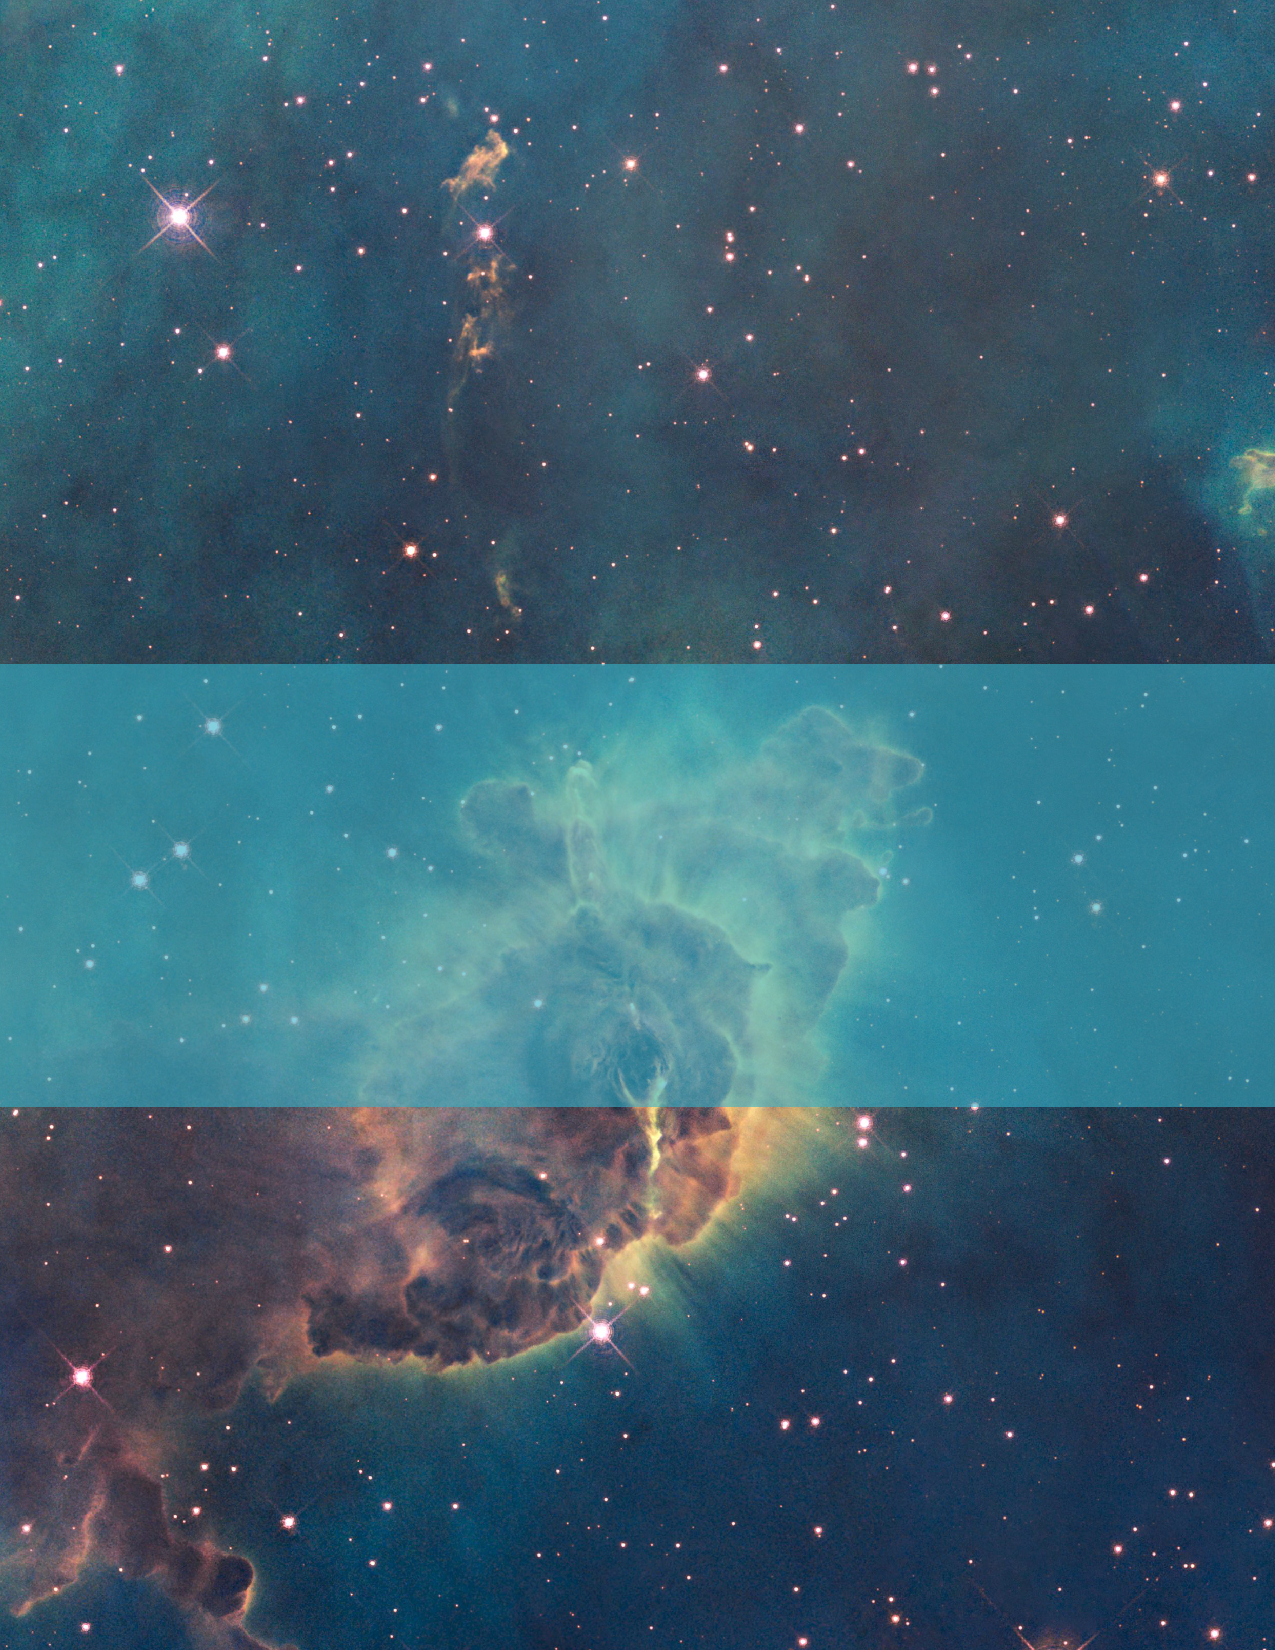
\includegraphics[scale=1.25]{Figures/esahubble}}} % Image background
\centering
\vspace*{5cm}
\par\normalfont\fontsize{35}{35}\sffamily\selectfont
\textbf{Εισαγωγή στην Αστροφυσική}\\
{\LARGE Σάββας Χανλαρίδης}\par % Book title
\vspace*{1cm}
{\Huge Σημειώσεις Μαθήματος}\par % Author name
\endgroup






    % \newcommand{\HRule}{\rule{\linewidth}{0.5mm}}
    % \center
    % % \textsl{\Huge Όνομα Σχολής}\\[0.5cm] 
    % % \textsl{\Large Όνομα Τμήματος}\\[2cm] 
    % \makeatletter
    % \HRule \\[0.6cm]
    % { \huge \bfseries \@title}\\[0.3cm] 
    % \HRule \\[2cm]
    % \large
    % \vspace{5cm}
    % \center 
    % 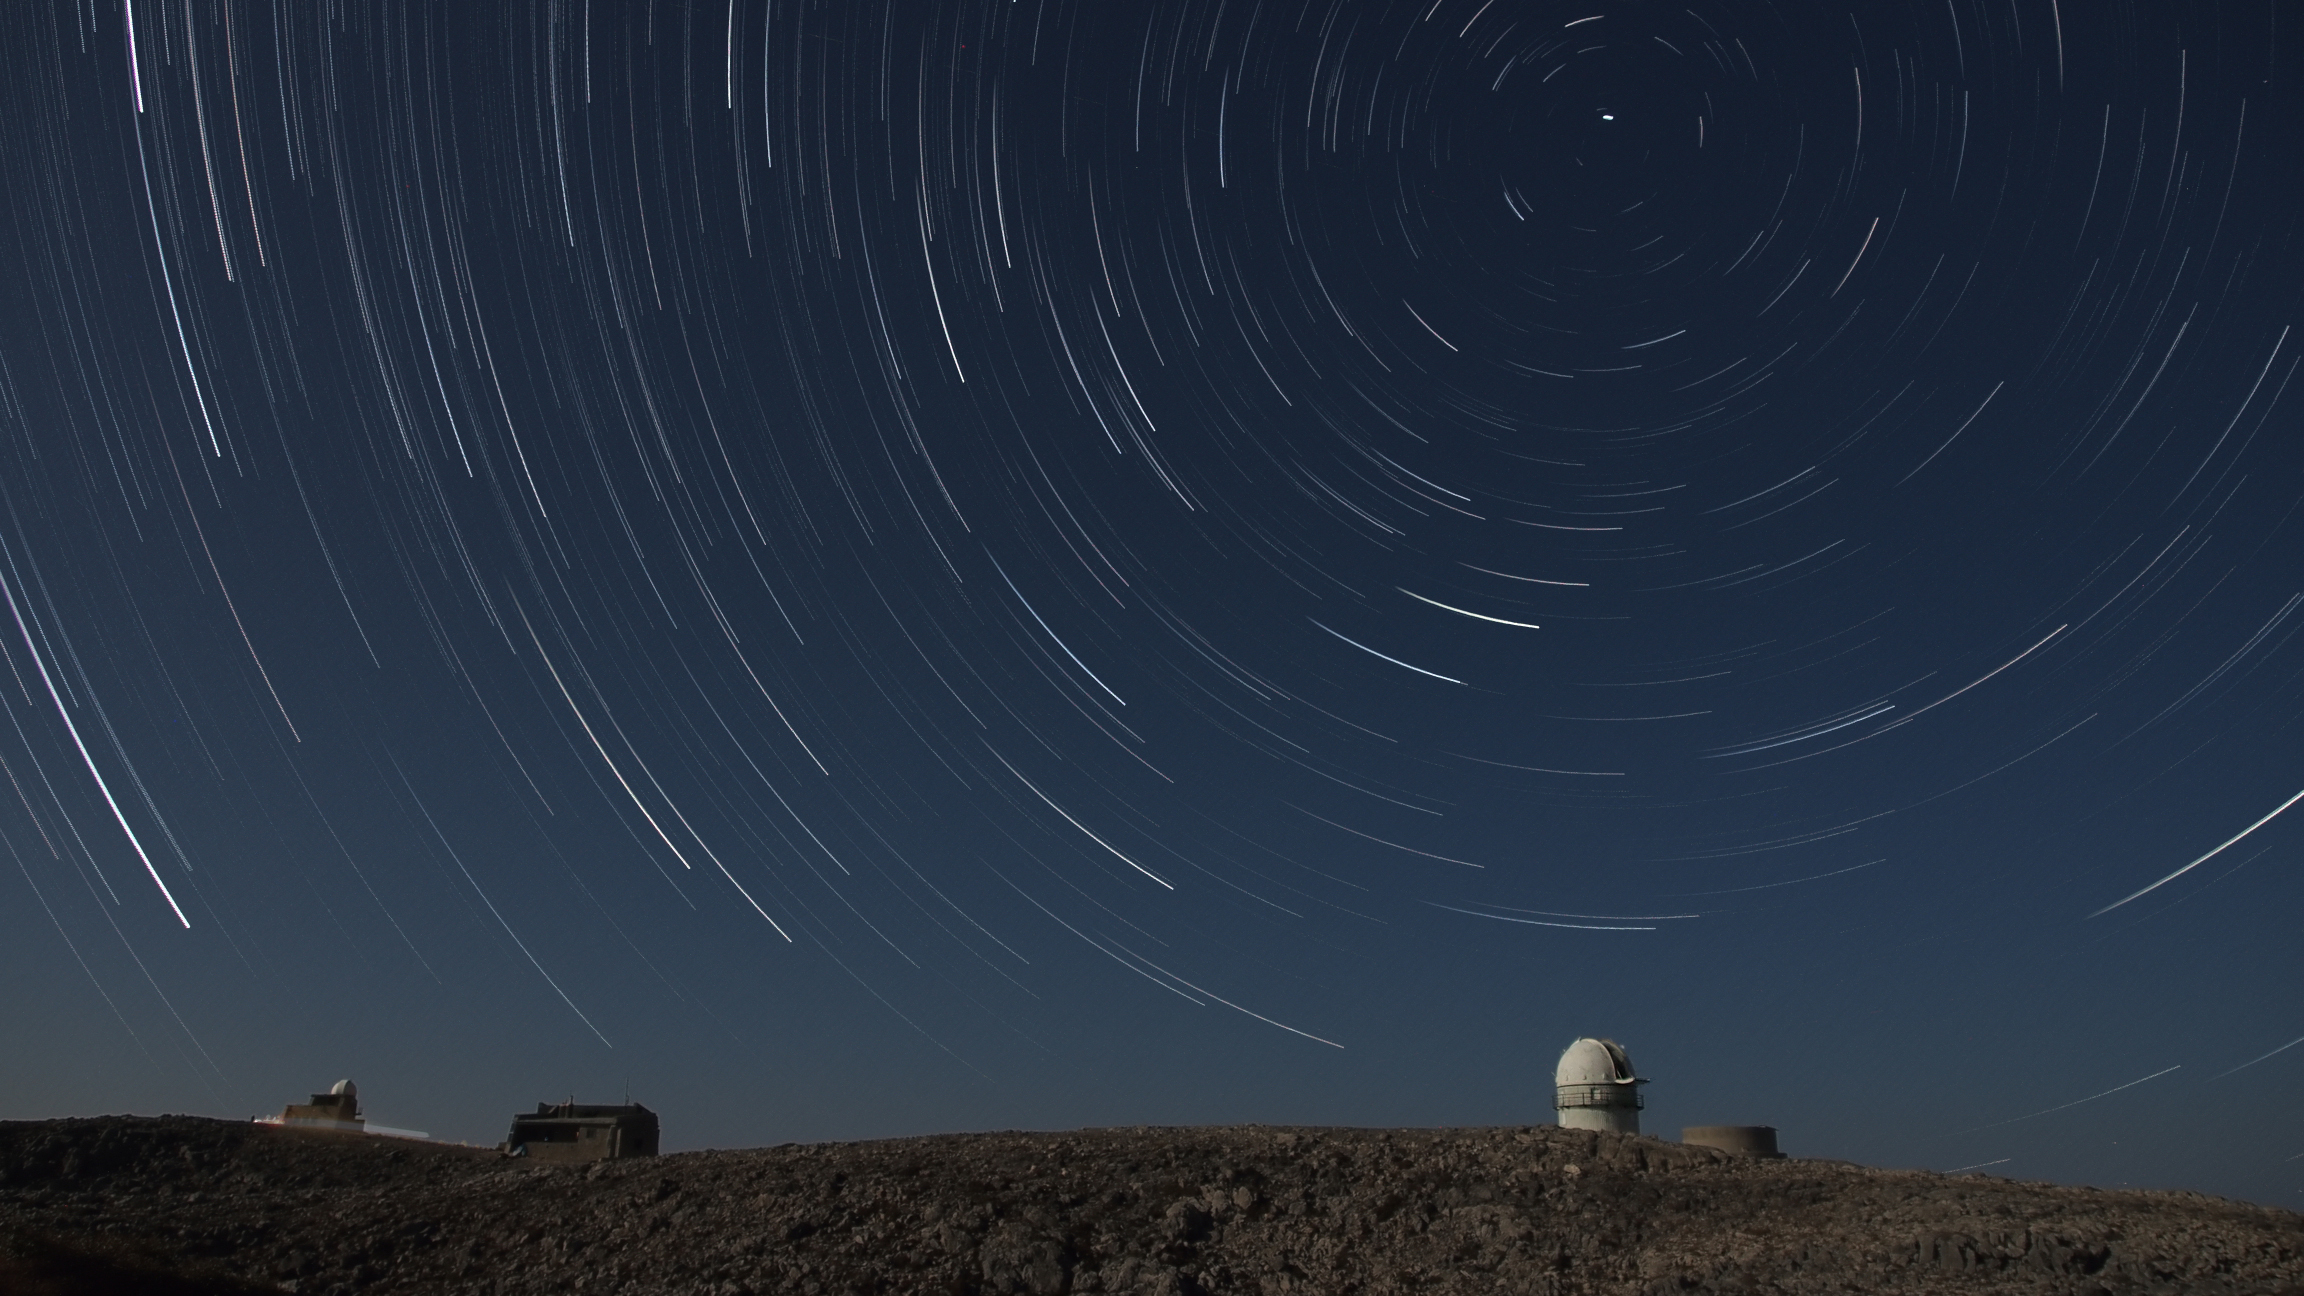
\includegraphics[width=\linewidth]{title/skinakas_star_trails.jpg}
    
   
    % \begin{minipage}{0.45\textwidth}
    % 	\begin{flushleft}
    %         \emph{Συγγραφέας:}\\
    %         \@author \\
    %     \end{flushleft}
    % \end{minipage}
    % ~
    % \begin{minipage}{0.45\textwidth}
    % 	\begin{flushright}
    %         \emph{Υπεύθυνος Καθηγητής:} \\
    %         \textup{Όνομα Καθηγητή}
    %     \end{flushright}
    % \end{minipage}\\[3cm]
    
    % \makeatother
    
    % {\large Η εργασία κατατέθηκε για το μάθημα:}\\[0.2cm]
    % {\Large \emph{Όνομα Μαθήματος}}\\[1cm]
    % {\large \today}\\[2cm]
    % \vfill 
    
\end{titlepage}
    
%     \selectlanguage{english}
    
%     % Define names of report parts
%     \renewcommand{\contentsname}{Περιεχόμενα}
%     \renewcommand{\listfigurename}{Λίστα Σχημάτων}
%     \renewcommand{\listtablename}{Λίστα Πινάκων}
%     \renewcommand{\chaptername}{Κεφάλαιο}
%     \renewcommand{\appendixname}{Παράρτημα}
%     \renewcommand{\bibname}{Βιβλιογραφία}
    
%     \pagenumbering{roman}
%     %\setlength{\parskip}{0.5em}     % Space between paragraphs
    

%     \tableofcontents
%     % \listoffigures
%     % \listoftables
    
%     \pagenumbering{arabic}
%     %\setlength{\parskip}{1em}       % Space between paragraphs

 
%     \chapter{Παρατηρησιακά χαρακτηριστικά αστέρων}
\label{ch:Chapter2}
	{\hypersetup{linkcolor=black, pdfborder=0 0 1}
% 	\adjustmtc
% 	\adjustmtc
	\minitoc
	%\newpage
	}

\section{Μέθοδος της παράλλαξης}
% Πόσο μακριά είναι τα αστέρια; %
% ----------------------------- %

Η μέτρηση αποστάσεων στο Σύμπαν ήταν ανέκαθεν ένα πολύ δύσκολο πρόβλημα. Με το πέρασμα των αιώνων και την ανάπτυξη τόσο της θεωρητικής κατανόησης του κόσμου όσο και νέων τεχνολογικών εφαρμογών, μπορέσαμε να βρούμε διάφορες τεχνικές που θα μας επέτρεπαν να λύσουμε το πρόβλημα της μέτρησης της απόστασης των αστρονομικών αντικειμένων. Η επιλογή της εκάστοτε τεχνικής μέτρησης εξαρτάται από την κλίμακα για την οποία ενδιαφερόμασατε. Για παράδειγμα, η μέτρηση της απόστασης αντικειμένων που βρίσκονται μέσα στο ηλιακό μας σύστημα γίνεται με τη βοήθεια των radar. Η μέθοδος αυτή βασίζεται στην αποστολή μίας δέσμη φωτονίων στα ραδιαφωνικά μήκη κύματος προς το αντικείμενο το οποίο θέλουμε να βρούμε την απόστασή του. Τα φωτόνια αυτά ανακλώνται από την επιφάνεια του αντικειμένου, επιστρέφουν σε εμάς και εφόσον γνωρίζουμε το χρονικό διάστημα που παρήλθε από τη στιγμή της εκπομπής του σήματος εώς τη λήψη του, η απόσταση θα δίνεται απλά:

\begin{equation}
    d = c (\delta t / 2)
\end{equation}
όπου $c$ είναι η ταχύτητα του φωτός και $\delta t$ το χρονικό διάστημα ανάμεσα στην εκπομπή και τη λήψη του σήματος.
\\

Αυτός ο τρόπος μέτρησης αποστάσεων ισχύει μόνο για αντικείμενα μέσα στο ηλιακό μας σύστημα και δεν μπορεί να χρησιμοποιηθεί για τον υπολογισμό αποστάσεων άλλων αστέρων. Λόγω των τεράστιων αποστάσεων, το σήμα θα έπρεπε να ταξιδεύει για χρόνια μέχρι να φτάσει (x2 μέχρι να γυρίσει) στον αστέρα.
Επίσης, το σήμα θα ήταν πολύ εξασθενημένο για να μετρηθεί πίσω στη Γη.



Μέσω αυτής της μεθόδου, ξέρουμε ότι η \textit{μέση} απόσταση Γης-Ήλιου είναι: $$1 \ \text{AU} \approx 149600000 \ \text{km}$$

Για να μετράμε αποστάσεις σχετικά κοντινών αστέρων, χρησιμοποιούμε την μέθοδο της τριγωνομετρικής \textit{παράλλαξης}. Η μέθοδος αυτή βασίζεται στην \textit{φαινόμενη} κίνηση ενός αντικειμένου σε σχέση με ένα πολύ πιο μακρινό υπόβαθρο (background) καθώς το κοιτάμε από διαφορετικές γωνίες. Με άλλα λόγια, η παράλλαξη είναι η φαινόμενη αλλαγή στη θέση ενός αντικειμένου βάσει μιας διαφορετικής οπτικής γωνίας.\\ 

\hrule
\textit{\underline{Παράδειγμα}}: Κρατήστε το δάχτυλό σας μπροστά από το πρόσωπό σας και παρατηρείστε το ανοιγοκλείνωντας ένα μάτι κάθε φορά. Όσο μεγαλύτερη είναι η απόσταση στην οποία τοποθετούμε το δάχτυλο, τόσο μικρότερη είναι η φαινόμενη μετατόπιση λόγω της διαφορετικής θέσης της παρατήρησης.
\hrule

Χρησιμοποιώντας την παραπάνω γεωμετρική ιδιότητα, παρατηρούμε ότι κοντινά αστέρια φαίνεται να μετατοπίζονται λόγω της κίνησης της Γης γύρω από τον Ήλιο (σχήμα \ref{fig:parallax}).

\begin{figure}[h]
    \centering
    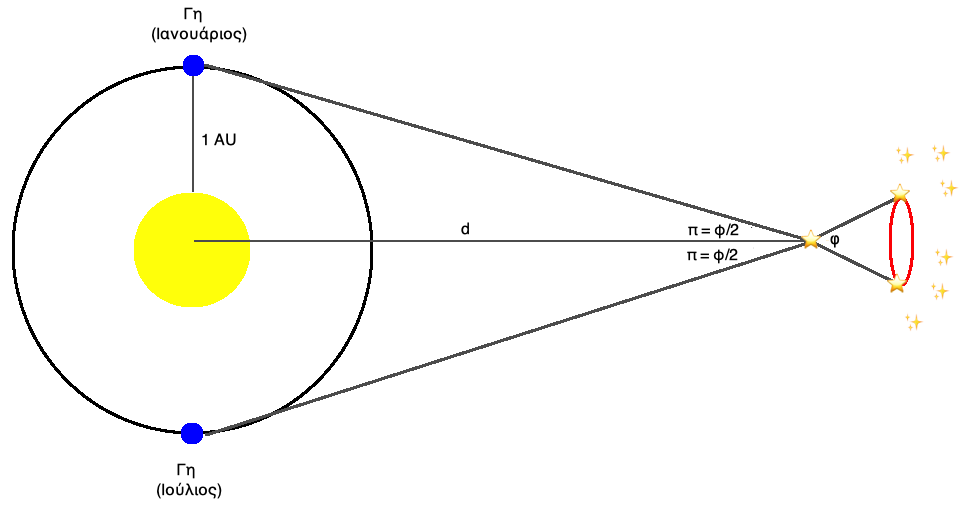
\includegraphics[width=\linewidth]{Figures/parallax.png}
    \caption{Ορισμός της ετήσιας (τριγωνομετρικής) παράλλαξης.}
    \label{fig:parallax}
\end{figure}

Μετράμε την θέση ενός στόχου-αστέρα και την ξαναμετράμε έπειτα από 6 μήνες όταν η Γη θα βρίσκεται στην αντιδιαμετρική θέση της τροχιάς της. Στη συνέχεια, μετράμε την αλλαγή στη φαινόμενη θέση του αστέρα σε σχέση με κάποια πολύ μακρινά άστρα στο υπόβαθρο που η φαινόμενη μετατόπισή τους είναι αμελητέα. Αυτή η αλλαγή περιγράφεται σε όρους "γωνία παράλλαξης", $p$. Για μία φαινόμενη μετατόπιση $\phi$, η απόσταση $d$ του στόχου δίνεται από:

\begin{equation}
    d = \frac{1 \ \text{AU}}{\tan p} \approx \frac{1 \ \text{AU}}{p}
\end{equation}
όπου στο δεύτερο μέρος χρησιμοποιήσαμε τη σχέση για μικρές γωνίες (small angle approximation) $\tan \theta \approx \theta$, όταν η γωνία $\theta$ μετριέται σε \textit{ακτίνια} (rad).

Η κόκκινη έλλειψη στο σχήμα υποδηλώνει την φαινόμενη ελλειπτική τροχιά που εκτελεί ο αστέρας πάνω στην ουράνια σφαίρα, λόγω της περιστροφής της Γης γύρω από τον Ήλιο. Αυτο το γεγονός είναι και μια άμεση απόδειξη ότι η Γη κινείται γύρω από τον Ήλιο και όχι το ανάποδο.

Το γεγονός ότι η τροχιά της Γης δεν ειναι απόλυτα σφαιρική δεν αποτελεί ιδιαίτερο πρόβλημα καθώς οι διακυμάνσεις στην ακτίνα της τροχιάς είναι πάρα πολύ μικρές συγκριτικά με την απόσταση $d$ των αστέρων. Άλλωστε, το σφάλμα στην μέτρηση της παράλλαξης είναι πολύ μεγαλύτερο από το σφάλμα που υπεισέρχεται εαν θεωρήσουμε ότι η ακτίνα της τροχιάς της Γης γύρω από τον Ήλιο δεν παραμένει σταθερή.


Γνωρίζουμε ότι $1 \ \text{rad} = 57.3^{\circ} = 206265 \ \text{arcsec}$. Μπορούμε να ορίσουμε έτσι, ένα νέο μέγεθος για μέτρηση μήκους, το \textit{parsec} (pc). Ένα parsec ορίζεται ως η απόσταση ενός αντικειμένου το οποίο πρέπει να έχει ώστε να παράγει παράλλαξη (parallax shift) ίση με 1 arcsec.

\begin{equation}
    1 \ \text{pc} = \frac{1 \ \text{AU}}{4.85 \times 10^{-6} \ \text{rad}} = 3.09 \times 10^{18} \ \text{cm} = 3.26 \ \text{ly}
\end{equation}

Έτσι, ισχύου οι σχέσεις:

\begin{equation}
    d = \frac{1 \ \text{AU}}{p \ (\text{rad})} = \frac{206265 \ \text{AU}}{p \ (\text{arcsec})} = \frac{1 \ \text{pc}}{p \ (\text{arcsec})}
\end{equation}
% \textit{\underline{ΠΡΟΣΟΧΗ}}: Η ΓΩΝΙΑ $\pi$ ΑΝΑΦΕΡΕΤΑΙ ΣΤΗΝ ΠΑΡΑΛΑΞΗ ΚΑΙ ΟΧΙ ΣΤΗΝ ΣΤΑΘΕΡΑ!
% \\
% {\color{red} \hrule }
% E: Γιατί να ορίσουμε το parsec με βάση παράλλαξη $\pi = 1 \ \text{arcsec}$;\\
% Α: Γιατί το κοντινότερο σε μας αστέρι (Εγγύτατος του Κενταύρου) έχει παράλλαξη $\pi \simeq 1 \ \text{arcsec}$, άρα όλα τα άλλα αστέρια είναι πολλαπλάσια του 1pc.
% {\color{red} \hrule }

\textit{\underline{Παράδειγμα}}: Ο εγγύτατος του Κενταύρου έχει παράλλαξη $ p = 0.77 \ \text{arcsec}$. Άρα η απόστασή του είναι:
\begin{equation*}
    d = \frac{1}{p \ \text{arcsec}} \text{pc} = \frac{1}{0.77} \ \text{pc} = 1.3 \ \text{pc} \simeq 267000 \ \text{AU}
\end{equation*}
\hrule



\section{Λαμπρότητα αστέρων}
% Πόσο λαμπρά είναι τα αστέρια; %
% ----------------------------- %

Η συντριπτική πλειοψηφία των πληροφοριών που έχουμε για τα αστέρια είναι μέσω της συλλογής φωτός σε διάφορα μήκη κύματος. Η έλλειψη φωτεινής πληροφορίας (ενώ ξέρουμε ότι έχει εκπεμφθεί) μας τροφοδοτεί με περαιτέρω πληροφορία για τις διαδικασίες απορρόφησης αυτής της μερίδας Η/Μ κυμάτων από τη μεσοαστρική ύλη.

Όταν μετράμε το φως που εκπέμπουν τα άστρα, μετράμε:
\begin{enumerate}
    \item την ένταση
    \item την πόλωση
\end{enumerate}

Η προφανής και πρώτη ερώτηση που μας έρχεται στο μυαλό είναι:
``Όλα τα αστέρια έχουν την ίδια λαμπρότητα, και γιατί;''. Ξερουμε ότι ενδογενώς, όλα τα αστέρια δεν έχουν την ίδια λαμπρότητα. Αλλά και την ίδια λαμπρότητα να είχαν, αυτό σημαίνει ότι θα φαινόντουσαν το ίδιο λαμπρά σε εμάς; Τι ρόλο παίζει η απόσταση σε αυτή την εικόνα; Είναι προφανές ότι πρέπει να ορίσουμε κάποιες ποσότητες που έχουν να κάνουν τόσο με την ενδογενή, όσο και με την φαινόμενη λαμπρότητα του αστέρα.

Ως \textit{λαμπρότητα} (L) ορίζουμε τη συνολική ισχύς (ενέργεια/χρόνο) που ακτινοβολείται από την επιφάνεια του αστέρα. Ως ισχύς, η λαμπρότητα μετριέται σε [W, erg/s]. Με άλλα λόγια, η λαμπρότητα εκφράζει τον ρυθμό με τον οποίο ένα αστέρι ακτινοβολεί ενέργεια. Η λαμπρότητα είναι μια ενδογενής ιδιότητα και μπορεί να υπολογισθεί από την \textit{φωτεινότητα} (ροή ή φαινόμενη λαμπρότητα), την ενέργεια δηλαδή της Η/Μ ακτινοβολίας που φτάνει στη Γη, και μπορεί να μετρηθεί άμεσα. Η φωτεινότητα εξαρτάται από την απόσταση του αστέρα από εμάς και ορίζεται από τη σχέση:

\begin{equation}
    F = \frac{L}{4 \pi d^2}
\end{equation}
όπου $d$ η απόσταση του αστέρα από τη Γη.

Η ποσότητα $4 \pi d^2$ ορίζει ουσιαστικά μία επιφάνεια σφαίρας με ακτίνα $d$ (σχήμα \ref{fig:flux}), και άρα η φωτεινότητα είναι μια ποσότητα που μετριέται σε [W/$\text{m}^2$, $\text{erg} \cdot \text{s}^{-1} \cdot \text{cm}^{-2}$]. Μπορούμε να πούμε δηλαδή ότι η φωτεινότητα ενός αστέρα είναι η ενέργεια ανα μονάδα χρόνου που διέρχεται από επιφάνεια $1 \ \text{m}^2$, \textit{ανεξάρτητα} της διεύθυνσης διάδοσης του φωτός.

\begin{figure}[h]
    \centering
    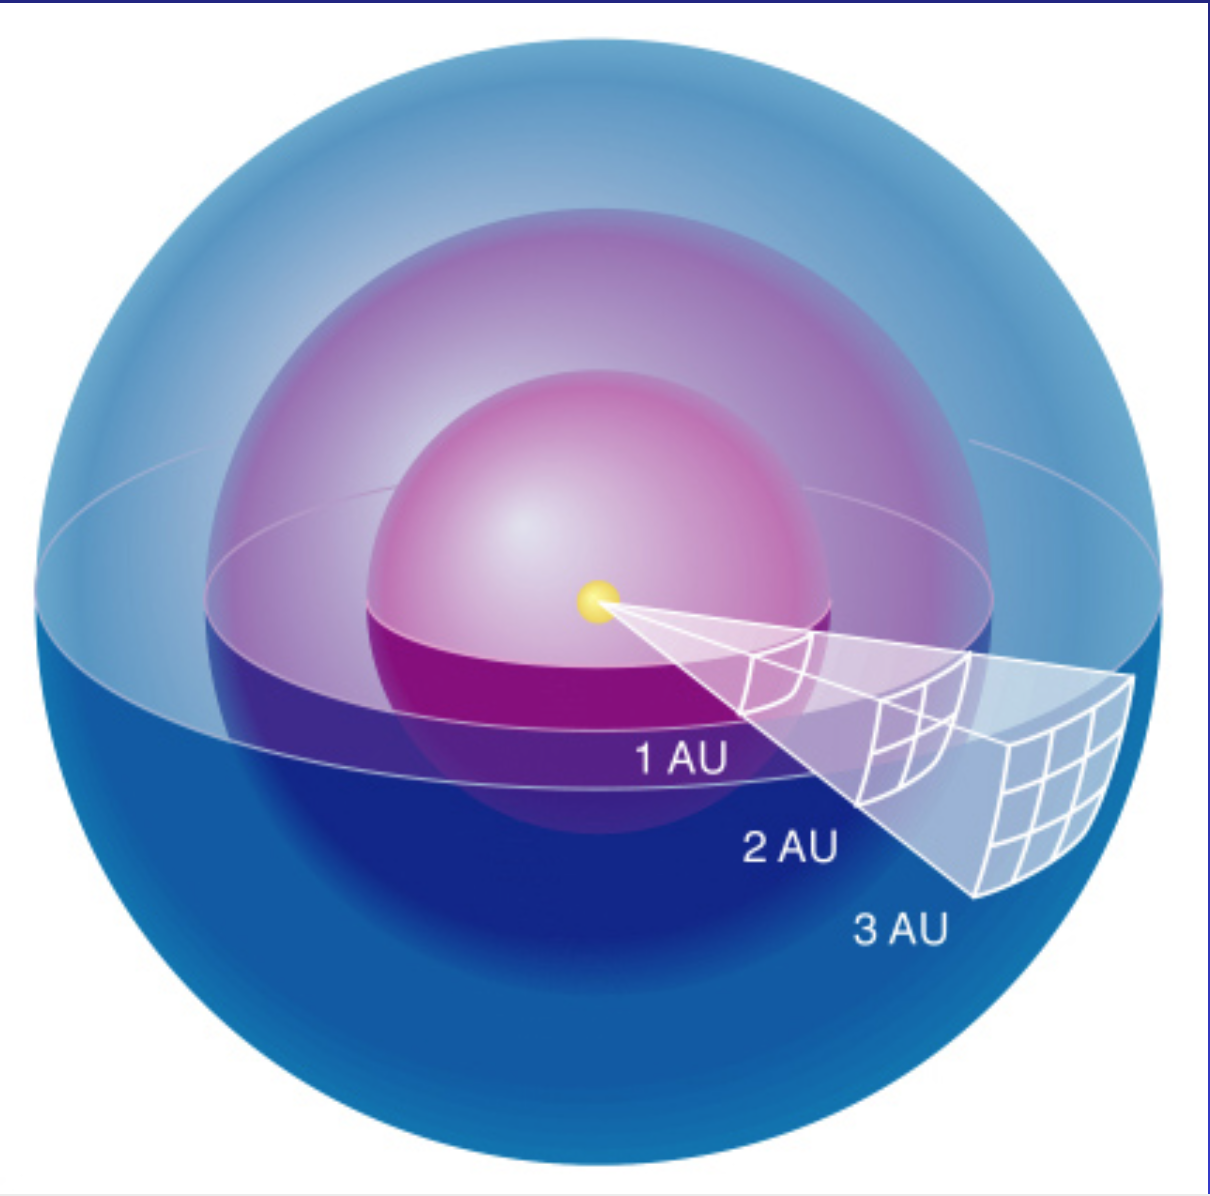
\includegraphics[scale=0.3]{Figures/flux.png}
    \caption{Φαινόμενη λαμπρότητα αστέρα και εξάρτησή της από την απόσταση.}
    \label{fig:flux}
\end{figure}

'Ενας τρόπος να ταξινομήσουμε τα αστέρια είναι ανάλογα με τη φωτεινότητά τους, δηλαδή με το πόσο λαμπρά φαίνονται στο ανθρώπινο μάτι (Ίππαρχος). Αργότερα, υιοθετήθηκε ένας μαθηματικός τύπος (Pogson) που μας δίνει το \textit{φαινόμενο μέγεθος} ενός αστέρα, δηλαδή του πόσο φωτεινός φαίνεται να είναι:

\begin{equation}
    \label{eq:apparent_magnitude}
    m = -2.5 \log \left ( \frac{F}{F_0} \right )
\end{equation}
όπου $F_0$ είναι μία σταθερά.

Παρατηρούμε ότι το μέγεθος ενός αστέρα δεν είναι τίποτα άλλο παρά η φωτεινότητά του εκφρασμένη σε λογαριθμική κλίμακα. Αυτό μας δίνει ένα μέτρο για τη μείωση της ροής της ακτινοβολίας λόγω της απόστασης, σύμφωνα με τον νόμο του αντίστροφου τετραγώνου.

Γιατί όμως το μέγεθος ως ποσότητα υπερτερεί έναντι της χρήσης της φωτεινότητας ως μέγεθος; Γιατί η φωτεινότητα ενός αστέρα που καταγράφει ένα τηλεσκόπιο εξαρτάται από το μέγεθος του κατόπτρου (ένα τηλεσκόπιο 10 μέτρων έχει δέκα φορές μεγαλύτερη συλλεκτική επιφάνεια από ένα τηλεσκόπιο 1 μέτρου), αλλά και από την ευαισθησία του εξοπλισμού (π.χ. μία μοντέρνα κάμερα μπορεί να καταγράφει περισσότερα φωτόνια ίδιας ενέργειας). Προκύπτει άρα η ανάγκη βαθμονόμησης. Η βαθμονόμηση αυτή γίνεται βάσει της φωτεινότητας του Vega ($F_0$) η οποία έχει γίνει σε πραγματικές μονάδες (W/$\text{m}^2$). Άρα χρησιμοποιώντας τον λόγο ($F/F_0$) προκύπτει ένα μέγεθος που δεν εξαρτάται από τον παρατηρησιακό εξοπλισμό.

Παραμένουν όμως οι ερωτήσεις: γιατί λογάριθμος, γιατί το μείον στη σχέση \eqref{eq:apparent_magnitude}, και γιατί ο συντελεστής 2.5; Γιατί να μην ορίζαμε το μέγεθος ως $m = F/F_0$ για παράδειγμα;

Λύνοντας την εξίσωση \eqref{eq:apparent_magnitude} για δύο αστέρες έχουμε:

\begin{eqnarray*}
    m_1 &=& -2.5 \log \left( \frac{F_1}{F_0} \right) \Rightarrow F_1 = F_0 \cdot 10^{-m_1/2.5} = F_0 \cdot 100^{-m_1/5} \\\\
    m_2 &=& -2.5 \log \left( \frac{F_2}{F_0} \right) \Rightarrow F_2 = F_0 \cdot 10^{-m_2/2.5} = F_0 \cdot 100^{-m_2/5}
\end{eqnarray*}
και διαιρώντας κατά μέλη παίρνουμε:

\begin{equation}
    \frac{F_1}{F_2} = 100^{(m_2 - m_1)/5}
\end{equation}

Παρατηρούμε ότι:
\begin{enumerate}
    \item αν οι δύο αστέρες διαφέρουν σε μέγεθος κατα 5, τότε η φωτεινότητά τους διαφέρει κατά έναν παράγοντα 100. Ο μαθηματικός που έκανε αυτή την παρατήρηση (Pogson), ήθελε να συνεχίσει την κλίμακα του Ίππαρχου όπου ένα αστέρι με μέγεθος 1 είναι 100 φορές πιο φωτεινό από ένα αστέρι με μέγεθος 6 ($\Delta m = 5$). Ο τρόπος για να το πετύχει αυτό ήταν να βάλει έναν παράγοντα 2.5 στη σχέση που συνδέει μέγεθος με φωτεινότητα, η οποία πρέπει να είναι λογαριθμική καθώς η ευαισθησία του ανθρώπινου ματιού στη φωτεινότητα μια πηγής είναι λογαριθμική.
    \item Αν $F_1 < F_2$ τοτε $m_1 > m_2$. Και πάλι, για να μην χαλάσει η ταξινόμηση του Ίππαρχου όπου τα πιο φωτεινά αστέρια είναι μικρότερου μεγέθους, προκύπτει το μείον στη σχέση \eqref{eq:apparent_magnitude}.
\end{enumerate}

Κατά αντιστοιχία, μπορούμε να ορίσουμε το \textit{απόλυτο μέγεθος}, M, ενός αστέρα ως το φαινόμενο μέγεθος (m) αν το αστέρι βρισκόταν σε απόσταση 10pc από εμάς.

\begin{eqnarray*}
    M &=& -2.5 \log \left( \frac{F_{10 \text{pc}}}{F_0} \right) \longrightarrow \frac{F_{10 \text{pc}}}{F} = 100^{(m-M)/5} \Rightarrow \\
    &\Rightarrow & \frac{\displaystyle L/4\pi (10 \text{pc})^2}{L/4 \pi d^2} = 100^{(m-M)/5} \Rightarrow d^2 = 100^{(m-M+5)/5} \Rightarrow \\\\
    & \Rightarrow & \boxed{d = 10^{(m-M+5)/5} \ \text{pc}}
\end{eqnarray*}
Λύνοντας ως προς $m-M$:

\begin{equation}
    \label{eq:distance_modulus}
    m-M = 5(\log d - 1)
\end{equation}

Η εξίσωση \eqref{eq:distance_modulus} είναι γνωστή ως \textit{distance modulus} και βάσει αυτής μπορούμε να υπολογίσουμε την απόσταση ενός αστέρα αν γνωρίζουμε το φαινόμενο και το πραγματικό μέγεθός του.

Στην περίπτωση που υπάρχει μεσοαστρική απορρόφηση, τότε η \eqref{eq:distance_modulus} γράφεται
\begin{equation}
    m - M - A = 5\log\,d - 5
\end{equation}
όπου $A$ είναι το μέγεθος της μεσοαστρικής απόσβεσης.

\section{Γωνιώδης απόσταση}
% Πόσο μεγάλα (σε όγκο) είναι τα αστέρια; %
% --------------------------------------- %
Υπάρχει ένας καθαρά γεωμετρικός τρόπος να υπολογίσει κανείς την ακτίνα ενός άστρου. Η μέθοδος αυτή βασίζεται στην \textit{γωνιακή διάμετρο} του αστέρα.

\begin{figure}[h]
    \centering
    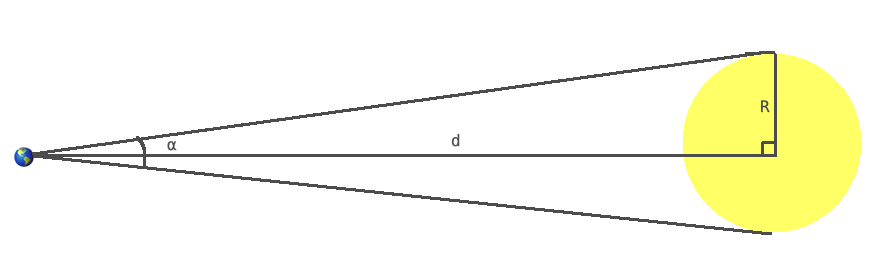
\includegraphics[scale=0.4]{Figures/angular_diameter.png}
    \caption{Γωνιακή διάμετρος α, ενός αστέρα. }
    \label{fig:angular_diameter}
\end{figure}

Από τη γεωμετρία του σχήματος \ref{fig:angular_diameter} παρατηρούμε ότι η γωνιακή διάμετρος α (κατά αναλογία, α/2 είναι η γωνιακή ακτίνα) θα δίνεται από τη σχέση:

\begin{equation}
    \label{eq:angular_diameter}
    \tan \left( \frac{\alpha}{2} \right) = \frac{R}{d}
\end{equation}
ενώ για μικρές γωνίες ισχύει: $\tan \theta \approx \sin \theta \approx \theta$, οταν η γωνία μετριέται σε ακτίνια.
\\

{\color{red} \hrule}
\textbf{Για τον Ήλιο}: $\alpha = 1919 \ \text{arcsec} = 31.98 \ \text{arcmin} = 0.53^{\circ} = 9.3 \times 10^{-3} \ \text{rad}$.

Άρα: $R_\odot = 1 \ \text{AU} \times \tan \left( \frac{0.53^{\circ}}{2}\right) \approx 0.0046 \ \text{AU}$

\textbf{Για τον Betelgeuse}: $\alpha = 0.125 \ \text{arcsec} = 0.0021 \ \text{arcmin} = 0.000035^{\circ}$, \\ $d=197 \ \text{pc} \simeq 4 \times 10^7 \ \text{AU} \ (\pm 45 \ \text{pc})$

Άρα: $R_B = (4 \times 10^7 \ \text{AU}) \times \tan \left( \frac{0.000035}{2} \right) \simeq 12 \ \text{AU} \Rightarrow R_B \simeq 2580 R_\odot$

O Betelgeuse είναι ένας υπεργίγαντας αστέρας με ακτίνα (και λαμπρότητα) κατά πολύ μεγαλύτερη από αυτή του Ήλιου.

\textbf{Για τον εγγύτατο του Κενταύρου}: $\alpha = 1 \times 10^{-3} \ \text{arcsec}$, $d = 1.3 \ \text{pc}$

Άρα: $R_{PC} \simeq 0.14 R_{\odot}$

Ο εγγύτατος του Κενταύρου είναι ένας νάνος αστέρας με ακτίνα (και λαμπρότητα) κατά πολύ μικρότερη από αυτή του Ήλιου.
{\color{red} \hrule}

Γίνεται αντιληπτό ότι ο άμεσος προσδιορισμός της γωνιακής διαμέτρου των αστέρων είναι εξαιρετικά δύσκολη υπόθεση λόγω της τεράστιας απόστασής τους.


\section{Σχέσεις $\rm L = f(M)$ και $\rm R = f(M)$}
Η πιο σημαντική θεμελιώδης ιδιότητητα, η μάζα, δεν μπορεί να μετρηθεί άμεσα για ένα απομονωμένο αστέρι. Για να μετρήσουμε αστρικές μάζες χρειαζόμαστε διπλά συστήματα αστέρων που παρουσιάζουν διακυμάνσεις στην ακτινική τους ταχύτητα (φασματοσκοπικά διπλοί αστέρες). Οι ακτινικές ταχύτητες από μόνες τους μπορούν να προσδιορίσουν μάζες μέχρι έναν παράγοντα $\sin i$, όπου $i$ είναι η γωνία κλίσης (inclination) της τροχιάς του διπλού συστήματος. Για τον προσδιορισμό απόλυτων τιμών της μάζας χρειαζόμαστε πληροφορίες για το $i$, είτε από ένα οπτικά διπλό σύστημα (visual binary) ή από την παρουσία εκλείψεων (eclipsing binary). Περισσότερα γι' αυτά τα συστήματα στο Κεφάλαιο  \ref{ch:Chapter7}. 

Από παρατηρήσεις άστρων στη γειτονιά του Ήλιου έχουμε καταφέρει να μετρήσουμε με ακρίβεια τις μάζες, τις λαμπρότητες και τις ακτίνες τους (σε διπλά συστήματα). Θα περίμενε κανείς να μην υπάρχει κανένας συσχετισμός μεταξύ αυτών των ποσοτήτων (λαμπρότητα και ακτίνα σχετίζονται μέσω του νόμου Stefan-Boltzmann οπως θα δούμε παρακάτω). Παρόλα αυτά, όταν κάνουμε τη γραφική παράσταση της λαμπρότητας με τη μάζα, και της ακτίνας με τη μάζα παρατηρούμε ότι υπάρχει ξεκάθαρα συχετισμός μεταξύ αυτών των ποσοτήτων (σχήμα \ref{fig:luminosity_mass_relation}).

\begin{figure}[h]
    \centering
    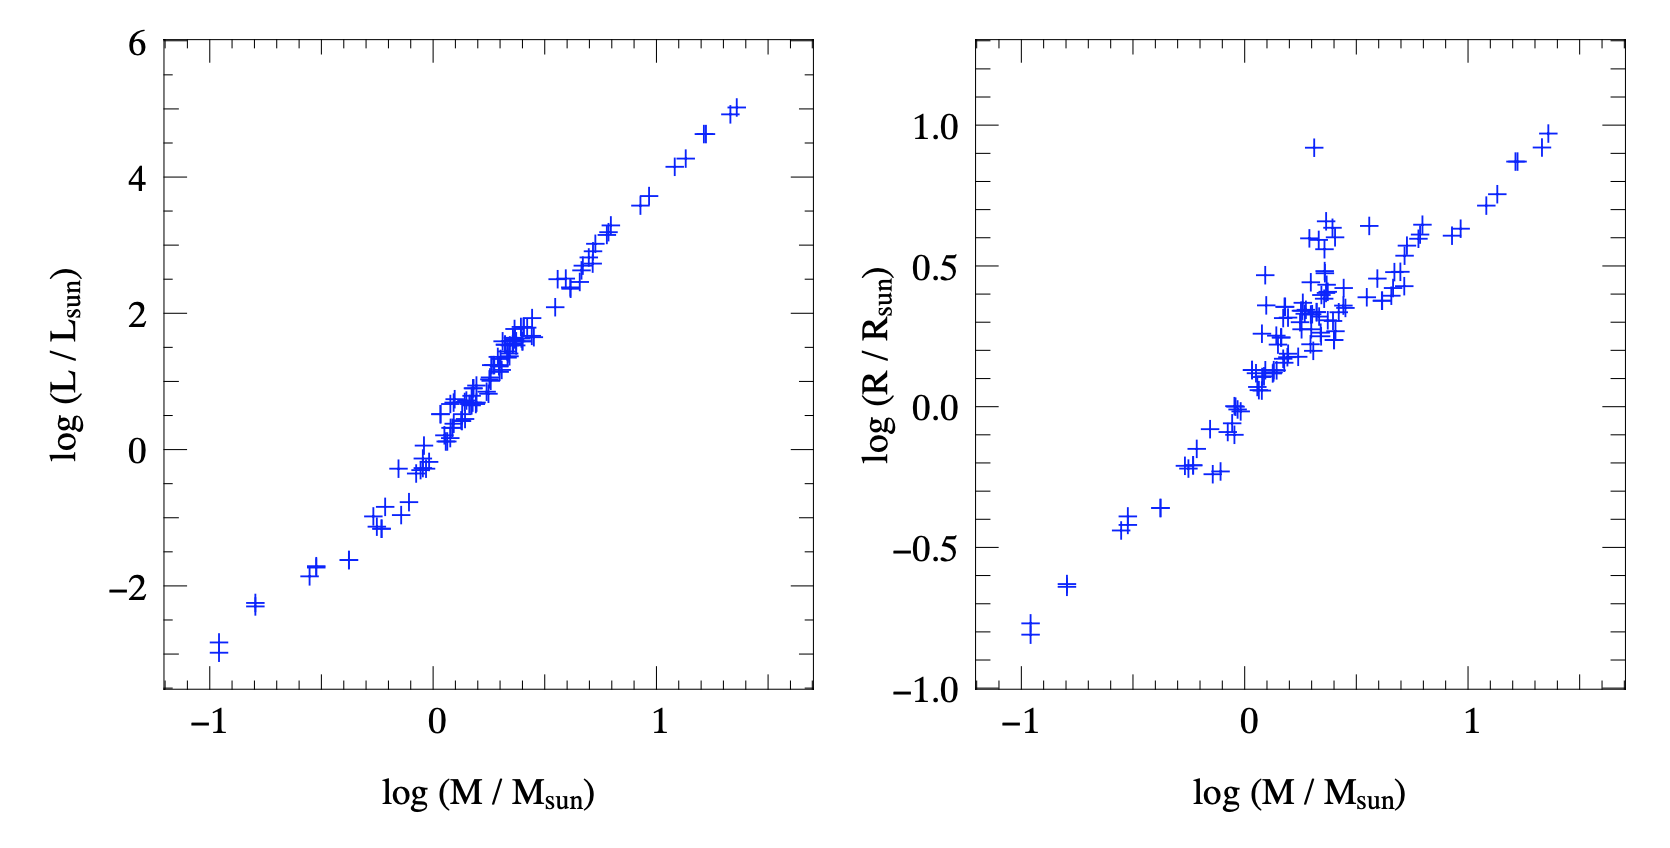
\includegraphics[width=\linewidth]{Figures/luminosity_mass_relation.png}
    \caption{Οι μάζες, ακτίνες και λαμπρότητες έχουν μετρηθεί με ακρίβεια $\lesssim 2 \,\%$ σε εκλειπτικά διπλούς αστέρες. Τα περισσότερα από αυτά τα αστέρια είναι αστέρες στην κύρια ακολουθία. Η διασπορά στις ακτίνες των αστέρων μεταξύ 1 και 2 $M_{\odot}$ οφείλεται στο γεγονός ότι αρκετά εξελιγμένα άστρα σε αυτό το εύρος μαζών, ικανοποιούν επίσης το κριτήριο της ακρίβειας της τάξης του $2 \,\%$.}
    \label{fig:luminosity_mass_relation}
\end{figure}

Αυτός ο παρατηρούμενος συσχετισμός μπορεί να προσεγγιστεί ικανοποιητικά καλά από τους εκθετικούς νόμους (power laws) των σχέσεων \eqref{eq:lum_mass} και \eqref{eq:radius_mass}.

\begin{equation}
    \label{eq:lum_mass}
    L \propto 
    \begin{cases}
        M^{2.5} & \text{εαν} \ M < 0.7 M_{\odot} \\\\
        M^{3.8} & \text{εαν} \ M > M_{\odot}
    \end{cases}
\end{equation}

\begin{equation}
    \label{eq:radius_mass}
    R \propto M^{0.7}
\end{equation}

Προφανώς, χρειαζόμαστε μία θεωρία αστρικής εξέλιξης η οποία να εξηγεί την ύπαρξη και τις κλίσεις αυτών των σχέσεων.


\section{Ακτινοβολία μέλανος σώματος}
% Πόσο ζεστά είναι τα αστέρια; %
% ---------------------------- %

% {\color{red} \hrule}
% Ε: Γιατί διάφορα αστέρια φαίνονται διαφορετικό χρώμα στον ουρανό; (π.χ. Rigel vs Betelegeuse)\\
% A: Επειδή έχουν διαφορετικές θερμοκρασίες. Αυτός ο συσχετισμός δεν είναι προφανής, αλλά όπως θα δείξουμε στη συνέχεια, η συχνότητα εκπομπής ενός αντικειμένου εξαρτάται \textit{μόνο} από τη θερμοκρασία του και όχι από άλλες παραμέτρους, όπως η σύστασή του.
% {\color{red} \hrule}

Σε καλή προσέγγιση μπορούμε να θεωρήσουμε ένα αστερι ως ένα μέλαν σώμα, εννοώντας ένα αντικείμενο που απορροφά \textit{όλο} το φως που πέφτει πάνω του. Τα μελανά σώματα έχουν την ιδιότητα ότι το φάσμα που εκπέμπουν εξαρτάται μόνο από τη θερμοκρασία τους, ενώ η εκπομπή γίνεται ισοτροπικά. Το φάσμα δεν είναι τίποτα άλλο παρά ένα γράφημα της έντασης της Η/Μ ακτινοβολίας προς το μήκος κύματος (σχήμα \ref{fig:black_body_spectrum}).

\begin{figure}[h]
    \centering
    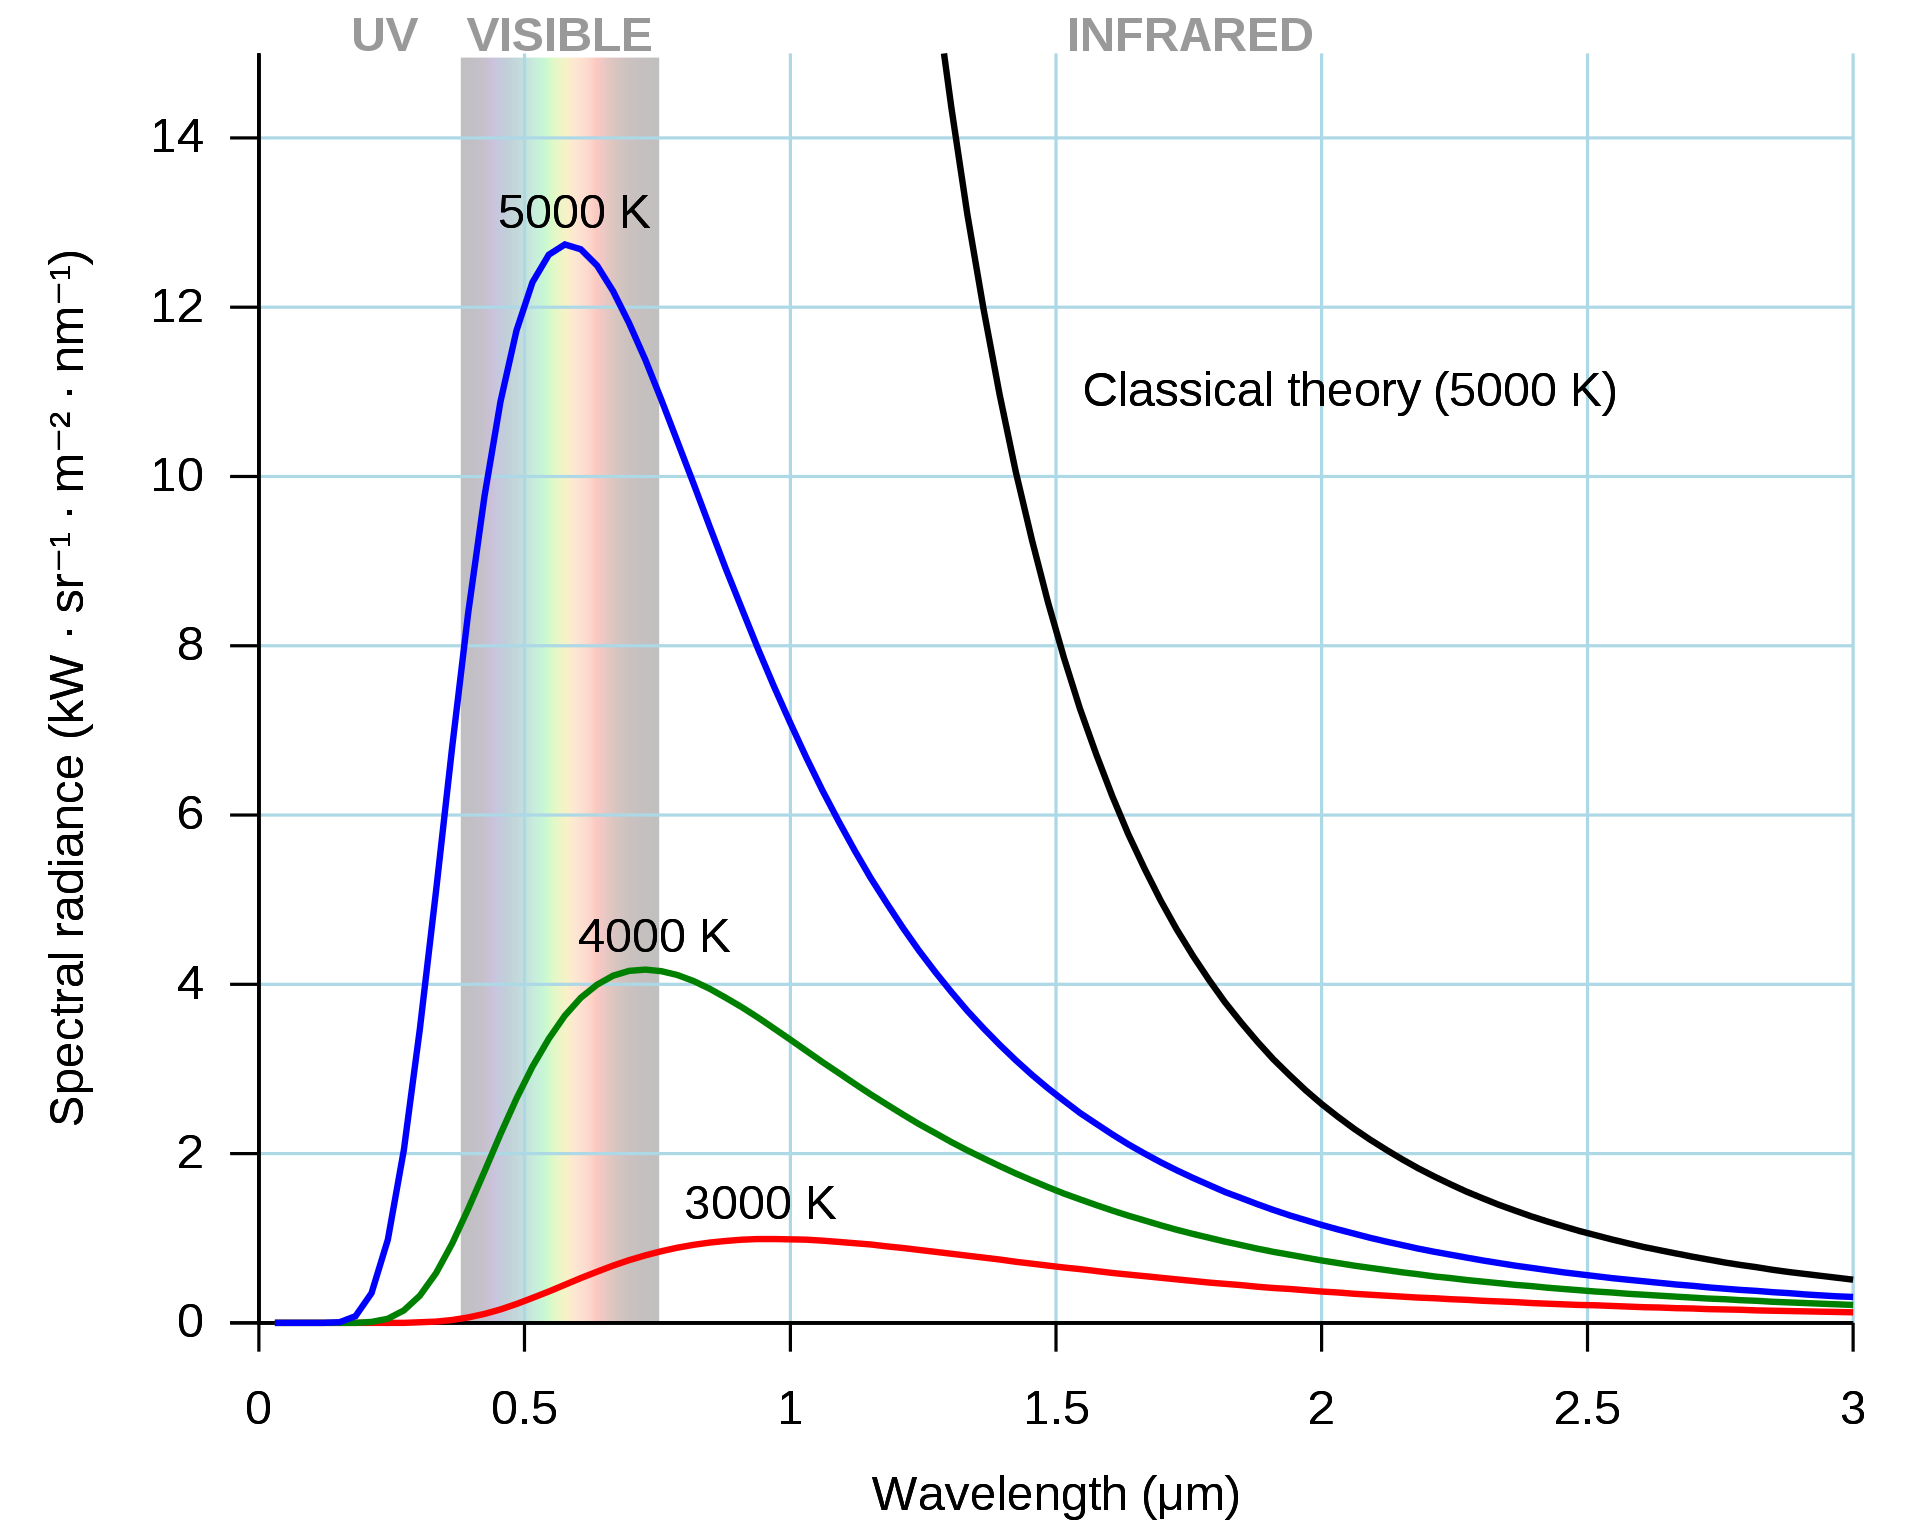
\includegraphics[width=\linewidth]{Figures/black_body_spectrum.png}
    \caption{Φάσμα εκπομπής μελανών σωμάτων διαφόρων θερμοκρασιών. Στα μικρά μήκη κύματος φαίνεται η υπεριώδης καταστροφή (UV catastrophe) όπως προκύπτει με την κλασική θεωρία των Rayleigh-Jeans.}
    \label{fig:black_body_spectrum}
\end{figure}

Παρατηρώντας τα φάσματα του σχήματος \ref{fig:black_body_spectrum} βλέπουμε ότι:

\begin{enumerate}
    \item Η ακτινοβολία μέλανου σώματος είναι συνεχής
    \item $T_1 < T_2 < T_3 \Rightarrow \lambda_1 > \lambda_2 > \lambda_3$
    Αυτό σημαίνει ότι υπάρχει ένα μήκος κύματος όπου η ακτινοβολία γίνεται μέγιστη και μάλιστα,  μέλανα σώματα υψηλότερης θερμοκρασίας εκπέμπουν ακτινοβολία μικρότερου μήκου κύματος.
    \item Οι καμπύλες δεν τέμνονται ποτέ! Ένα μέλαν σώμα υψηλότερης θερμοκρασίας θα εκπέμπει \underline{πάντα} περισσότερη ακτινοβολία συγκριτικά με ένα μέλαν σώμα χαμηλότερης θερμοκρασίας. Το μόνο που συμβαίνει είναι ότι το μέγιστο της εκπομπής μετακινείται σε υψηλότερα μήκη κύματος.
\end{enumerate}

\subsection{Νόμος του Planck}
Ποιά είναι όμως η συνάρτηση που δίνει τις καμπύλες (φάσμα) ενός μέλανος σώματος;
Η ένταση του φωτός που παράγει ένα μέλαν σώμα θερμοκρασίας Τ σε μήκος κύματος $\lambda$, δίνεται από τη σχέση του Planck:

\begin{equation}
    \label{eq:planck_function_lambda}
    B_{\lambda}(T) = \frac{2hc^2}{\lambda^5} \frac{1}{\exp(hc/\lambda kT) - 1}
\end{equation}

Η παραπάνω σχέση είναι γνωστή ως \textit{νόμος του Planck}. Μπορούμε να εκφράσουμε το νόμο του Planck με όρους συχνότητας, αλλά δεν αρκεί η αντικατάσταση του μήκους κύματος με τη συχνότητα σύμφωνα με τη θεμελιώδη σχέση $\nu \lambda = c$. Αυτό που πρέπει να θυμόμαστε είναι ότι ο νόμος του Planck εκφράζει ενέργεια ανα μονάδα χρόνου, ανα επιφάνεια, ανα μήκος κύματος (ή συχνότητα), και ανα στερεά γωνία. Οπότε πρέπει να ισχύει:

\begin{eqnarray*}
    B_{\lambda} (T) &=& \frac{dE}{dt \cdot dA \cdot d \lambda \cdot d \Omega} \\ 
    B_{\nu} (T) &=& \frac{dE}{dt \cdot dA \cdot d \nu \cdot d \Omega} \\\\
    &\text{ή}& \\\\
    |B_{\lambda} (T) d \lambda | &=& |B_{\nu} (T) d \nu |
\end{eqnarray*}
Άρα αν ολοκληρώσουμε σε όλα τα μήκη κύματος/συχνότητες παίρνουμε την ολική ενέργεια που εκπέμφθηκε. Αλλά: $$\nu \lambda = c \Rightarrow \nu = \frac{c}{\lambda} \Rightarrow |d\nu | = | d \left( c / \lambda \right) | \Rightarrow | d\nu | = \left | \frac{c}{\lambda^2}d\lambda \right |$$

Τελικά έχουμε:

\begin{eqnarray}
\label{eq:planck_function_frequency}
    B_{\nu}(T) &=& \frac{B_{\lambda}(T) d \lambda}{d\nu} \Rightarrow B_{\nu}(T) = \frac{B_{\lambda}(T) \cancel{d\lambda}}{\displaystyle  \frac{c}{\lambda^2} \cancel{d \lambda}} =  \frac{\lambda^2}{c} \frac{2hc^2}{\lambda^5} \frac{1}{\exp(hc / \lambda kT) - 1} \Rightarrow \nonumber \\ \nonumber \\
    &\Rightarrow & B_{\nu}(T) =  \frac{2hc}{\lambda^3} \frac{1}{\exp(hc / \lambda kT) - 1} =  \frac{2hc}{c^3 / \nu^3} \frac{1}{\exp(h \nu / kT) - 1} \Rightarrow \nonumber \\ \nonumber \\
    &\Rightarrow & \boxed{B_{\nu}(T) =  \frac{2h \nu^3}{c^2} \frac{1}{\exp(h \nu / kT) - 1}}
\end{eqnarray}


\subsection{Νόμος του Wien}
Αν διαφορίσουμε τη συνάρτηση του Planck (σχέση \eqref{eq:planck_function_lambda}) ως προς μήκος κύματος και τη θέσουμε ίση με μηδέν, παρατηρούμε ότι φτάνει ένα μέγιστο σε μήκος κύματος:
$$\frac{d B_{\lambda}(T)}{d \lambda} = 0 \Rightarrow \lambda_{\text{max}} = 0.2 \frac{hc}{kT} = \frac{0.29}{T} \ \text{cm}$$

\begin{equation}
    \boxed{\lambda_{\text{max}} \cdot T = 0.003 \ \text{mK}}
\end{equation}

Άρα το μήκος κύματος στο οποίο η εκπομπή ακτινοβολίας είναι μέγιστη εξαρτάται \underline{μόνο} από τη θερμοκρασία $\longrightarrow$ άρα δεν έχουν όλα τα αστέρια την ίδια επιφανειακή θερμοκρασία.

\subsection{Νομος των Stefan-Boltzmann}
Ολοκληρώνοντας αυτή τη φορά τον νόμο του Planck για όλες τις συχνότητες, προκύπτει ότι:

\begin{equation}
    \label{eq:stefan_boltzmann}
    L = A \sigma T^4 \Rightarrow \boxed{L = 4 \pi R^2 \sigma T_{\text{eff}}^4}
\end{equation}
όπου $A$ είναι η επιφάνεια μέλανος σώματος, και για αστέρα ακτίνας $R$ ισχύει $A=4\pi R^2$. Ο παράγοντας $T_{\text{eff}}^4$ ονομάζεται \textit{ενεργός θερμοκρασία} του αστέρα και ορίζεται ως η θερμοκρασία που θα έπρεπε να έχει ένα μέλαν σώμα ώστε να παράγει την ίδια ροή ενέργειας που παράγει η επιφάνεια του αστέρα. Με άλλα λόγια η ενεργός θερμοκρασία προσεγγίζει ικανοποιητικά την θερμοκρασία της επιφάνειας του αστέρα.

Γίνεται αντιληπτό ότι αν γνωρίζω την απόσταση ενός αστέρα (π.χ. μέσω της παράλλαξης), την φωτεινότητά του (με φωτομετρικές παρατηρήσεις) μπορώ να υπολογίσω τη λαμπρότητά του. Γνωρίζοντας την λαμπρότητα του αστέρα και μετρώντας την $T_{\text{eff}}^4$ (νόμος Wien) μπορώ να έχω μία εκτίμηση για την ακτίνα του αστέρα μέσω της σχέσης \eqref{eq:stefan_boltzmann}.

Τέλος, η εκπεμπόμενη ροή ακτινοβολίας από την επιφάνεια του αστέρα θα είναι:

\begin{eqnarray}
    F_{\text{surface}} = \frac{L}{4 \pi R^2} = \frac{\cancel{4 \pi R^2} \sigma T_{\text{eff}}^4}{\cancel{4 \pi R^2}} \Rightarrow F_{\text{surface}} = \sigma T_{\text{eff}}^4
\end{eqnarray}
%     \chapter{Φωτομετρία}
\label{ch:Chapter3}

\section{Φίλτρα και βολομετρικά μεγέθη}
% Συστήματα φίλτρων, ορισμός βολομετρικών μεγεθών, βολομετρική διόρθωση, υπεροχή χρώματος κτλ. %

\underline{Ορισμός βολομετρικών μεγεθών}

\begin{itemize}
    \item Ολική (ή βολομετρική) φωτεινότητα αστέρων 
    $$F_{\text{bol}} = \int_0^{\infty}F(\lambda) d\lambda = \frac{L_{\text{bol}}}{4 \pi d^2} = \frac{4\pi R^2 \sigma T_{\text{eff}}^4}{4\pi d^2}$$
    Το $F(\lambda)$ είναι το παρατηρούμενο φάσμα του αστέρα. Στο βαθμό που ο αστέρας συμπίπτει με μέλαν σώμα είναι ουσιαστικά το $B_{\lambda}$ της σχέσης του Planck.
    \item Ολικό (ή βολομετρικό) \textit{φαινόμενο} μέγεθος αστέρα 
    $$m_{\text{bol}} = -2.5 \log \left( \frac{F_{\text{bol}}}{F_{\odot}} \right) = 2.5 \log F_{\odot} - 2.5 \log F_{\text{bol}}$$
    
    {\color{red} Στην περίπτωση που μιλάμε για βολομετρικά μεγέθη, η σταθερά βαθμονόμησης ορίζεται βάσει της φωτεινότητας του Ήλιου και όχι του Vega!}
    \item Ολικό (ή βολομετρικό) \textit{απόλυτο} μέγεθος αστέρα
    $$M_{\text{bol}} = m_{\text{bol}} \ \text{όταν} \ d = 10 \ \text{pc} \longrightarrow M_{\text{bol}} = -2.5 \log \left( \frac{F_{\text{bol}, 10 \text{pc}}}{F_{\odot}} \right)$$
\end{itemize}

\textbf{Γνωρίζοντας ότι το απόλυτο βολομετρικό μέγεθος του Ήλιου είναι $M_{\odot}^{\text{bol}} = 4.74$, βρείτε μία σχέση που να συνδέει το απόλυτο μέγεθος ενός αστέρα με την λαμπρότητά του καθώς και αυτή του Ήλιου.}

Εξ' ορισμού το απόλυτο βολομετρικό μέγεθος του Ήλιου θα είναι
$$M_{\odot}^{\text{bol}} = -2.5 \log \left( \frac{F_{\odot, \text{10pc}}^{\text{bol}}}{F_{\odot}} \right) \Rightarrow 2.5 \log F_{\odot} - 2.5 \log F_{\odot, \text{10pc}}^{\text{bol}} = 4.74 $$

Για έναν τυχαίο αστέρα, το απόλυτο βολομετρικό μέγεθός του θα είναι κατά αντιστοιχία
$$M_{\text{bol}} = 2.5 \log F_{\odot} - 2.5 \log F_{\text{bol, 10pc}}$$

Πρέπει να εμφανίσουμε τον όρο $F_{\odot, \text{10pc}}^{\text{bol}}$, το οποίο το καταφέρνουμε με το να τον προσθαφαιρέσουμε από τη σχέση του απόλυτου βολομετρικού μεγέθους του αστέρα μας. Έτσι έχουμε:

\begin{eqnarray*}
    M_{\text{bol}} &=& {\color{green} 2.5 \log F_{\odot}} - 2.5 \log F_{\text{bol, 10pc}} + 2.5 \log F_{\odot, \text{10pc}}^{\text{bol}} - {\color{green} 2.5 \log F_{\odot, \text{10pc}}^{\text{bol}}} = \\\\
    &=& {\color{green}4.74} - 2.5 \log F_{\text{bol, 10pc}} + 2.5 \log F_{\odot, \text{10pc}}^{\text{bol}} \Rightarrow \\\\
    &\Rightarrow & 4.74 - M_{\text{bol}} = 2.5 \log \left[ \frac{L_{\text{bol}}}{4\pi (\text{10pc})^2} \right] - 2.5 \log \left[ \frac{L_{\odot}}{4\pi (\text{10pc})^2} \right] = \\\\
    &=& 2.5 \log \left( \frac{L_{\text{bol}}}{L_{\odot}} \right) \Rightarrow 0.4(4.74 - M_{\text{bol}}) = \log \left( \frac{L_{\text{bol}}}{L_{\odot}} \right) \Rightarrow \\\\
    &\Rightarrow & \boxed{\frac{L_{\text{bol}}}{L_{\odot}} = 10^{0.4(4.74 - M_{\text{bol}})}}
\end{eqnarray*}

Βάσει αυτής της σχέσης, μπορούμε να υπολογίσουμε αμέσως πόσες φορές πιο φωτεινός είναι ένας αστέρας από τον Ήλιο, αν γνωρίζουμε το απόλυτο μέγεθός του. \\
\hrule 

Ο υπολογισμός συνολικών φωτεινοτήτων είναι πολύπλοκη διαδικασία και εξαιρετικά χρονοβόρα όταν μελετάμε συστήματα με χιλιάδες αστέρια, π.χ. σφαιρωτά σμήνη. Η συλλογή φωτός σε όλα τα μήκη κύματος, η προσαρμογή τους σε μέλανα σώματα κτλ για κάθε ένα από τα μέλη ενός σμήνους είναι απαγορευτική.
Γι' αυτό το λόγο χρησιμοποιούμε φίλτρα (ηθμούς) τα οποία μας επιτρέπουν την παρατήρηση σε ένα συγκεκριμένο εύρος συχνοτήτων/μηκών κύματος.

Υπάρχουν πολλά συστήματα φίλτρων όπως π.χ. το ``Johnson-Cousins''. Σε αυτό το σύστημα υπάρχουν 5 φίλτρα, τα U, B, V, R, I. Το διάγραμμα (σχήμα \ref{fig:filter_curves}) δείχνει τις \textit{καμπύλες διαπερατότητας} $S(\lambda)$ αυτών των φίλτρων.

\begin{figure}
    \centering
    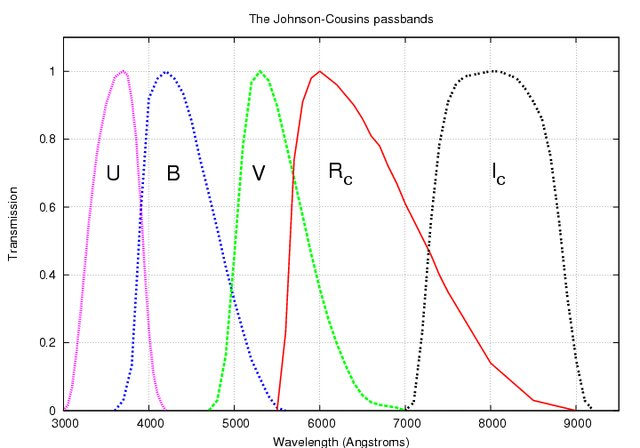
\includegraphics[width=\linewidth]{Figures/filter_curves.jpg}
    \caption{Καμπύλες διαπερατότητας για το σύστημα φίλτρων Johnson-Cousins. Ο άξονας y δείχνει την \textit{διαφάνεια}. Το φίλτρο V (visual) αφήνει να καταγραφούν τα ίδια φωτόνια (πάνω-κάτω) με αυτά που αντιλαμβάνονται τα μάτια μας. Δηλαδή με άλλα λόγια, η καμπύλη φασματικής ευαισθησίας του φίλτρου V είναι παρόμοια μ' εκείνη του ματιού μας.}
    \label{fig:filter_curves}
\end{figure}

Όταν παρατηρούμε ένα αστέρι μέσω ενός φίλτρου (π.χ. το V) τότε εμείς μετράμε:
\begin{equation}
    F_V = \int_0^{\infty} F(\lambda) S_V(\lambda) d\lambda
\end{equation}
όπου $F(\lambda)$ είναι το φάσμα που επέμπει ο αστέρας, και $S_V(\lambda)$ είναι η καμπύλη φασματικής ευαισθησίας, του φίλτρου και του ανιχνευτή.

Έτσι, μπορούμε να ορίσουμε τα μεγέθη ενός αστέρα στα διάφορα φίλτρα ως εξής:
\begin{eqnarray*}
    V \equiv m_V = -2.5 \log \left( \frac{F_V}{F_{V,0}} \right) = 2.5 \log F_{V,0} - 2.5 \log F_V = C_V - 2.5 \log F_V \\\\
    B \equiv m_B = -2.5 \log \left( \frac{F_B}{F_{B,0}} \right) = 2.5 \log F_{B,0} - 2.5 \log F_B = C_B - 2.5 \log F_B \\\\
    U \equiv m_U = -2.5 \log \left( \frac{F_U}{F_{U,0}} \right) = 2.5 \log F_{U,0} - 2.5 \log F_U = C_U - 2.5 \log F_U 
\end{eqnarray*}
όπου οι σταθερές $C_V, C_B, C_U$ κτλ ορίζονται με βάση τη φωτεινότητα του Vega στα αντίστοιχα μήκη κύματος, δηλαδή:
\begin{eqnarray*}
    C_V  &=& 2.5 \log(F_{V, Vega}) \\\\
    C_B  &=& 2.5 \log(F_{B, Vega}) \\\\
    C_U  &=& 2.5 \log(F_{U, Vega}) \hspace{1cm} \text{κτλ}
\end{eqnarray*}
Αυτό σημαίνει ότι εξ' ορισμού ισχύει $\boxed{m_{V,Vega} = m_{B,Vega} = m_{U,Vega} = \dots = 0}$
\\
{\color{red} \hrule} 
Ε: Ποιό είναι το βολομετρικό μέγεθος ενός αστέρα αν υποθέσουμε ότι εκπέμπει μόνο στα U,B,V,R;
Α: Αν κάποιος υποθέσει ότι το συνολικό μέγεθος $m_{\text{bol}}$ είναι απλώς το άθροισμα των επιμέρους μεγεθών στα διάφορα φίλτρα, τότε είναι λάθος! Με άλλα λόγια: $$m_{\text{bol}} \neq m_U + m_B + m_V + m_R$$
γιατί το μέγεθος είναι λογαριθμική ποσότητα. Αυτό που ισχύει είναι ότι η \textit{συνολική ροή θα ισούται με το άθροισμα των ροών στα αντίστοιχα φίλτρα}. Έτσι, αν γνωρίζουμε τα $m_U, m_B$ κτλ και θέλουμε να βρούμε το $m_{\text{bol}}$ dουλεύουμε ως εξής:
$$m_B = -2.5 \log \left( \frac{F_B}{F_{B,0}} \right) \Rightarrow -0.4m_B = \log \left( \frac{F_B}{F_{B,0}} \right) \Rightarrow F_B = F_{B,0} 10^{-0.4m_B}$$
Παρόμοια βρίσκουμε και τα $F_U, F_V, F_R$ και άρα $F_{\text{bol}} = F_B+F_V+F_U+F_R$. Τελικά $$m_{\text{bol}} = -2.5 \log \left( \frac{F_{\text{bol}}}{F_0} \right)$$
{\color{red} \hrule} 

Ο υπολογισμός της συνολικής φωτεινότητας ενός αστέρα είναι ο λόγος που κάνουμε παρατηρήσεις με περισσότερα από ένα φίλτρα. Παρόλα αυτά, υπάρχει και ένας άλλος τρόπος υπολογισμού, μέσω του $m_V$ και μόνο. Για αυτό τον λόγο θα πρέπει να ορίσουμε μία νέα ποσότητα η οποία είναι γνωστή ως \textit{βολομετρική διόρθωση} (bolometric correction) ή αλλιώς συντελεστής συνολικής διόρθωσης ως εξής:
\begin{equation}
    \boxed{BC = m_{\text{bol}} - m_V = M_{\text{bol}} - M_V}
\end{equation}

Η ιδέα για το BC είναι ότι {\color{blue}μπορεί να υπολογιστεί θεωρητικά}. Γνωρίζοντας ότι για τα περισσότερα άστρα το φάσμα τους προσαρμόζεται αρκετά ικανοποιητικά από το φάσμα ενός μέλανος σώματος, αν εγώ ξέρω τη θερμοκρασία ενός αστέρα, άρα ξέρω και το φάσμα του μέλανος σώματος που αντιστοιχεί σε αυτή τη θερμοκρασία, μπορώ να ολοκληρώσω το φάσμα ως προς όλα τα μήκη κύματος για να βρω την ολική λαμπρότητα του αστέρα, να ολοκληρώσω μετά το φάσμα μόνο στην περιοχή του φίλτρου V, και να υπολογίσω θεωρητικά τη ποσότητα BC για διάφορες θερμοκρασίες.

Άρα, παρατηρώντας το $m_V$ ενός αστέρα, μπορούμε να προσθέσουμε το BC που αντιστοιχεί στη θερμοκρασία του αστέρα (το οποίο έχει υπογισθεί θεωρητικά) και έτσι έχουμε μία εκτίμηση για το ολικό μέγεθος του αστέρα.
\\
{\color{red} \hrule}
\textbf{Για τον Ήλιο}: $M_{\text{bol}} = 4.74$ και $M_V = 4.83$. Άρα, $BC = -0.09$.
Παρατηρούμε ότι ο BC πρέπει πάντα να είναι αρνητικός καθώς τα μεγέθη ορίζονται με ένα μείον (μικρότερο μέγεθος συνεπάγεται πιο φωτεινός ο αστέρας).

\textbf{Για αστέρια με $T_{\text{eff}} \simeq 6700 \ \text{K}$} έχουμε $BC \simeq 0$. Αυτό σημαίνει ότι το $\lambda_{\text{max}}$ που αντιστοιχεί σε αυτή τη θερμοκρασία, δηλαδή το μεγαλύτερο μέρος της εκπεμπόμενης ακτινοβολίας διέρχεται μέσω του φίλτρου V.

\textbf{Για αστέρια με $T_{\text{eff}} > 6700 \ \text{K}$} το $\lambda_{\text{max}}$ μετατοπίζεται σε μικρότερα μήκη κύματος και άρα ``χάνουμε'' φωτόνια από εκεί.

\textbf{Για αστέρια με $T_{\text{eff}} < 6700 \ \text{K}$} αντίστοιχα, ``χάνουμε'' φωτόνια από τα μεγαλύτερα μήκη κύματος.
{\color{red} \hrule}

\underline{Παρατήρηση}: Βολομετρική διόρθωση μπορεί να οριστεί και σε άλλα μήκη κύματος πέρα του ορατού. Για παράδειγμα, σε μερικά ψυχρά άστρα όπου το μέγιστο της ενέργειάς τους εκπέμπεται στα υπέρυθρα μήκη κύματος, μπορούμε να εφαρμόσουμε ένα διαφορετικό σύνολο βολομετρικών διορθώσεων στο απόλυτο μέγεθος στα υπέρυθρα, αντί για το απόλυτο μέγεθος στα ορατά μήκη κύματος. Έτσι, $BC_K = M_{\text{bol}} - M_K$, όπου $BC_K$ και $M_K$ είναι η βολομετρική διόρθωση και το απόλυτο μέγεθος στην K-band αντίστοιχα.  
\hrule

Αφού λοιπόν θα μας αρκούσαν παρατηρήσεις μόνο σε ένα φίλτρο για να υπολογίσουμε τη συνολική φωτεινότητα ενός αστέρα, προκύπτει η εύλογη απορία τι μας χρειάζεται να παρατηρούμε στα άλλα φίλτρα. Η απάντηση είναι επειδή θέλουμε να υπολογίσουμε την επιφανειακή θερμοκρασία, $T_{\text{eff}}$ ενός αστέρα (χωρίς να χρειαστεί να έχουμε το συνολικό φάσμα του αστέρα), γνώση που είναι απαραίτητη για να βρούμε το BC.

\begin{figure}[h]
    \centering
    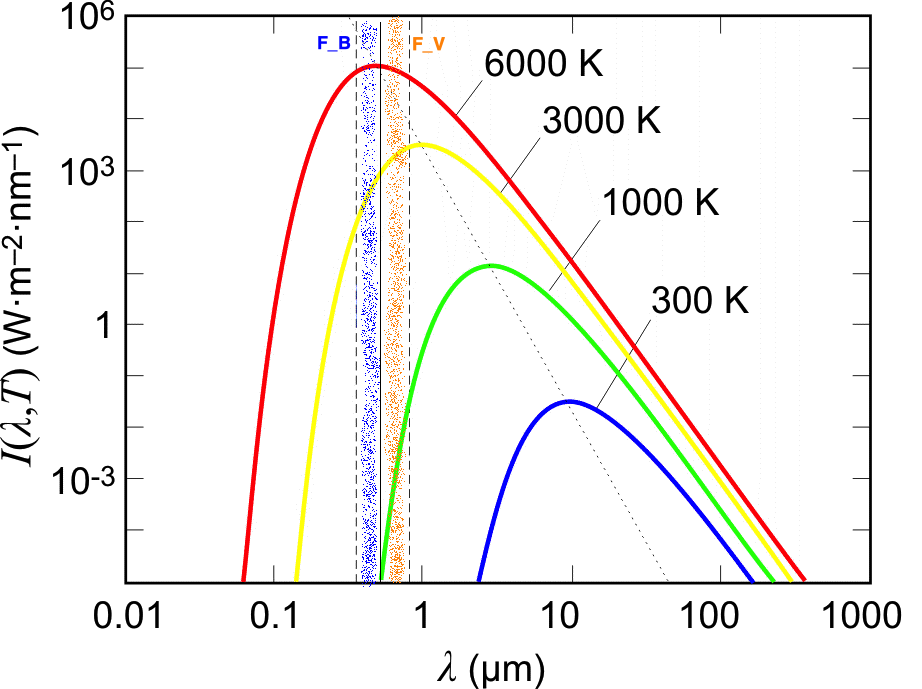
\includegraphics[width=\linewidth]{Figures/Planck_law_log_log_scale.png}
    \caption{Φάσματα μέλανων σωμάτων για διάφορες θερμοκρασίες. Το διάγραμμα είναι σε λογαριθμικούς άξονες γι' αυτό η μορφή των καμπυλών είναι διαφορετική.}
    \label{fig:planck_law_log_scale}
\end{figure}

Στο διάγραμμα \ref{fig:planck_law_log_scale} απεικονίζεται --ποιοτικά-- το εύρος των συχνοτήτων που καλύπτει το φίλτρο B (με μπλε χρώμα), ενώ με πορτοκαλί φαίνεται το εύρος συχνοτήτων που καλύπτει το φίλτρο V. {\color{blue} Άρα, η ροή του αστέρα στο φίλτρο B θα είναι το εμβαδόν της επιφάνειας που ορίζεται κάτω από την καμπύλη καθώς από τον ορισμό ξέρουμε ότι είναι το ολοκλήρωμα ως προς τα μήκη κύματος επι τη φασματική ευαισθησία του φίλτρου. Λόγω της μορφής των καμπυλών τα εμβαδά αυτά δεν είναι σταθερά}.

Αυτό που μας ενδιαφέρει είναι το εμβαδόν (η ροή) και στα δύο φίλτρα. Αν πάρουμε ως παράδειγμα το μέλαν σώμα θερμοκρασίας 6000 Κ, παρατηρούμε ότι το εμβαδόν στο B φίλτρο είναι ελαφρώς μεγαλύτερο από το εμβαδόν στο V φίλτρο. Άρα η διαφορά στα μεγέθη $B - V \equiv m_B - m_V < 0$ καθώς $F_B > F_V$.
Για το μέλαν σώμα θερμοκρασίας 3000 Κ, το εμβαδόν στο V φίλτρο είναι μεγαλύτερο από το εμβαδόν στο B φίλτρο. Άρα $B - V > 0$ καθώς $F_B < F_V$.
{\color{red} Η διαφορά στα μεγέθη των δύο φίλτρων δεν θα έχει το ίδιο πρόσημο! Έτσι, μετρώντας τη ροή του αστέρα σε δύο φίλτρα και παίρνοντας τη διαφορά στα μεγέθη τους, μπορούμε να υπολογίσουμε τη θερμοκρασία του αστέρα.}

\underline{Για να συνοψίσουμε}:\\
Χρειαζόμαστε παρατηρήσεις σε 2 τουλάχιστον φίλτρα. Παίρνοντας την διαφορά $B - V$, $U - V$ κτλ, βρίσκουμε τη θερμοκρασία του αστέρα. Γνωρίζοντας τη θερμοκρασία, έχουμε μία τιμή για τη βολομετρική διόρθωση που χρειαζόμαστε και κατά συνέπεια μπορούμε να υπολογίσουμε τη συνολική λαμπρότητα του αστέρα (αν γνωρίζουμε την απόσταση).

Αυτές οι διαφορές στα μεγέθη (π.χ. $B - V$) ονομάζονται ``\textit{δείκτες χρώματος}'' και συνήθως ορίζονται ως η διαφορά μεγέθους σε μικρότερο μήκος κύματος μείον το μέγεθος σε μεγαλύτερο μήκος κύματος. Συνηθισμένοι δείκτες χρώματος είναι οι $$B - V \equiv m_B - m_V, U - B \equiv m_U - m_B, V - R \equiv m_V - m_R$$

Θεωρώντας ότι ένα αστέρι εκπέμπει ως μέλαν σώμα, μπορούμε για κάθε θερμοκρασία να υπολογίσουμε θεωρητικά τι δείκτη χρώματος περιμένουμε. Στην πράξη, χρησιμοποιούμε διάφορες εμπειρικές σχέσεις όπως την παρακάτω για τον δείκτη $B-V$: 
\begin{equation}
    T_{\text{eff}} = \frac{9000 \ \text{K}}{(B - V) + 0.93}
\end{equation}
που ισχύει για αστέρια με δείκτη χρώματος $-0.1 \leq B-V \leq 1.4$ ή ισοδύναμα $4000 \ \text{K} \leq T_{\text{eff}} \leq 11000 \ \text{K}$.

\begin{itemize}
    \item Για τον Vega, $T_{\text{eff}} \approx 10000 \ \text{K}$ και εξ' ορισμού $B-V = U-B = \dots = 0$.
    \item Για αστέρια με $T_{\text{eff}} > 10000 \ \text{K} \longrightarrow B-V < 0$, ενώ για αστέρια με $T_{\text{eff}} < 10000 \ \text{K} \longrightarrow B-V > 0$. Αυτό το συμπέρασμα προκύπτει εύκολα αν σκεφτούμε ότι μεγαλύτερη θερμοκρασία συνεπάγεται $\lambda_{\text{max}}$ σε μικρότερη μήκη κύματος και άρα $F_B > F_V \Rightarrow m_B < m_V \Rightarrow B-V < 0$. Αντίστοιχη λογική ακολουθείται και για όταν $T_{\text{eff}} < 10000 \ \text{K}$.
\end{itemize}


\textbf{Ας υποθέσουμε ότι έχουμε ένα αστέρι ψυχρότερο από τον Vega και ότι ισχύει $\displaystyle \frac{F_B}{F_V} < \left( \frac{F_B}{F_V} \right)_{Vega}$. Να δείξετε ότι σε αυτή την περίπτωση $B-V > 0$.}

Γνωρίζουμε ότι 
\begin{eqnarray*}
\frac{F_B}{F_V} &<& \frac{F_{B,Vega}}{F_{V,Vega}} \Rightarrow \log \left( \frac{F_B}{F_V} \right) < \log \left( \frac{F_{B,Vega}}{F_{V,Vega}} \right) \Rightarrow \\\\\
&\Rightarrow & - \log \left( \frac{F_B}{F_V} \right) > - \log \left( \frac{F_{B,Vega}}{F_{V,Vega}} \right) \Rightarrow \\\\
&\Rightarrow & - 2.5 \log \left( \frac{F_B}{F_V} \right) > - 2.5 \log \left( \frac{F_{B,Vega}}{F_{V,Vega}} \right) \Rightarrow \\\\
&\Rightarrow & - \log \left( \frac{F_B}{F_V} \right) + \log \left( \frac{F_{B,Vega}}{F_{V,Vega}} \right) > 0 \Rightarrow \\\\
&\Rightarrow & {\color{green} -2.5 \log F_B} + {\color{purple} 2.5 \log F_V} + {\color{green} 2.5 \log F_{B,Vega}} {\color{purple} - 2.5 \log F_{V,Vega}} > 0 \Rightarrow \\\\
&\Rightarrow & -2.5 \left( \log F_B - \log F_{B,Vega} \right) + 2.5 \left( \log F_V - \log F_{V,Vega} \right) > 0 \Rightarrow \\\\
&\Rightarrow & \underbrace{-2.5 \log \left( \frac{F_B}{F_{B,Vega}} \right)}_{m_B} + \underbrace{2.5 \log \left( \frac{F_V}{F_{V,Vega}} \right)}_{- m_V} > 0 \Rightarrow \\\\
&\Rightarrow & m_B - m_V > 0 \Rightarrow \boxed{B - V > 0}
\end{eqnarray*}
\hrule 

Υπάρχει όμως λόγος να μελετάμε τα άστρα σε παραπάνω από 2 φίλτρα; Η απάντηση είναι πως ναι, καθώς μέχρι τώρα υποθέσαμε ότι δεν παρεμβάλεται τίποτα μεταξύ του παρατηρητή και του αστέρα. Στην πραγματικότητα, και ιδιαίτερα για τα άστρα που βρίσκονται στο γαλαξιακό επίπεδο, υπάρχουν αέρια και σκόνη που απορροφούν μέρος του φωτός.

Η απορρόφηση του οπτικού φωτός από τη μεσοαστρική σκόνη γίνεται με διαφορετικό τρόπο στα διάφορα μήκη κύματος. Η απορρόφηση είναι μεγαλύτερη στα μικρότερα μήκη κύματος (στο ``μπλε'' φως) οπότε τα αστέρια εμφανίζονται περισσότερο κόκκινα απ 'οτι είναι στην πραγματικότητα. Αυτό το φαινόμενο ονομάζεται ``\textit{μεσοαστρική ερυθρή χρώση}'' (interstellar reddening). Αν όμως έχουμε μετρήσεις του μεγέθους των αστέρων σε διάφορα φίλτρα, τότε μπορούμε να υπολογίσουμε την απορρόφηση στα διάφορα μήκη κύματος, να διορθώοσυμε τους παρατηρούμενες δείκτες χρώματος, και άρα να υπολογίσουμε τη σωστή $T_{\text{eff}}$ και τον συντελεστή βολομετρικής διόρθωσης BC.


Λόγω του φαινομένου της μεσοαστρικής ερυθρής χρώσης, ένας αστέρας παρατηρείται πιο κόκκινος απ' ότι είναι στην πραγματικότητα, δηλαδή με αλλοιωμένο δείκτη χρώματος. Αν $(B-V)$ είναι ο παρατηρούμενος και $(B-V)_0$ ο πραγματικός δείκτης χρώματος, τότε η διαφορά τους
\begin{equation}
    E_{(B-V)} = (B-V) - (B-V)_0
\end{equation}
ονομάζεται ``\textit{υπεροχή χρώματος}'' (color excess). Από την υπεροχή χρώματος υπολογίζεται τελικά η απορρόφηση σε αστρικά μεγέθη ($A_{\text{V}}$ για το οπτικό και $A_{\text{B}}$ για το κυανό) από τις εμπειρικές σχέσεις
\begin{align}
    A_{\text{V}} & = 3 E_{(B-V)} \\\nonumber\\
    A_{\text{B}} & = 4 E_{(B-V)}
\end{align}


\section{Φασματική ανάλυση}
Στα μέσα του 19ου αιώνα οι Kirchhoff και Bunsen παρατήρησαν ότι τα φάσματα των φυσικών σωμάτων ακολουθούν τους εξής δύο γενικούς κανόνες:
\begin{enumerate}
    \item Τα στερεά και τα υγρά σώματα εκπέμπουν συνεχές φάσμα, ενώ τα (αραιά) αέρια εκπέμπουν γραμμικό φάσμα.
    \item Όταν ένα αέριο παρεμβάλλεται μεταξύ μιας (θερμότερης από αυτό) πηγής συνεχούς φάσματος και του παρατηρητή, δημιουργούνται γραμμές απορρόφησης στο συνεχές φάσμα. Οι γραμμές αυτές έχουν το ίδιο μήκος κύματος με τις γραμμές εκπομπής του φάσματος του αερίου του κανόνα (1).
\end{enumerate}

Σε αυτό το κεφάλαιο θα αναλύσουμε κάποια χαρακτηριστικά των αστρικών φασμάτων δίνοντας έμφαση στο σχηματισμό της γραμμικής συνιστώσας, ενώ το πως μια αέρια μάζα --όπως ένας αστέρας-- μπορεί να έχει και συνεχές φάσμα, που έρχεται σε αντίθεση με τον κανόνα (1), θα γίνει αντιληπτό στο επόμενο κεφάλαιο.

\subsection{Αστρικά φάσματα}

Μπορούμε να πάρουμε το φάσμα μιας πηγής χρησιμοποιώντας ένα πρίσμα ή ένα φράγμα περίθλασης. Παρόλο που η λειτουργία των δύο αυτών οργάνων βασίζεται σε εντελώς διαφορετικά φυσικά φαινόμενα, τα αποτελέσματα που μας δίνουν είναι τα ίδια: αναλύουν μία παράλληλη πολυχρωματική δέσμη φωτός, σε μία αποκλίνουσα δέσμη, σε κάθε διεύθυνση της οποίας αντιστοιχεί φως μια συγκεκριμένης συχνότητας. Στη συνέχεια το φάσμα καταγράφεται φωτογραφικά ή φωτοηλεκτρικά.

Το φάσμα μιας πηγής χωρίζεται σε δύο συνιστώσες: τη \textbf{συνεχής} συνιστώσα και τη \textbf{γραμμική} συνιστώσα. Η τελευταία αποτελείται από \textbf{φασματικές γραμμές}, δηλαδή στενές φασματικές περιοχές πλάτους $\Delta \lambda$, όπου $\Delta \lambda \ll \lambda$, στις οποίες η φωτεινή ένταση έχει τιμή πολύ μεγαλύτερη (φωτεινές γραμμές) ή πολύ μικρότερη (σκοτεινές γραμμές) από τη μέση τιμή των γειτονικών της περιοχών.
Η συνεχής συνιστώσα αποτελείται από την εξομαλυμένη καμπύλη που προκύπτει αν ``αφαιρέσουμε'' από το φάσμα τις φασματικές γραμμές, ή αν ``προσαρμόσουμε'' στην πειραματική καμπύλη του φάσματος μια συνεχής ``θεωρητική'' καμπύλη σύμφωνα με κάποιο λογικό κριτήριο. Τέτοια θεωρητική καμπύλη μπορεί να είναι για παράδειγμα μία καμπύλη Planck (μέλανος σώματος) αν έχουμε λόγους να πιστεύουμε ότι το φωτοβόλο σώμα εκπέμπει θερμικά\footnote{Θερμική ακτινοβολία είναι η ακτινοβολία που εκπέμπεται από ένα σώμα λόγω της θερμικής του κατάστασης και η έντασή της περιγράφεται από τον νόμο του Planck.} και βρίσκεται σε θερμοδυναμική ισορροπία, ένα πολυώνυμο αν πιστεύουμε ότι το σώμα εκπέμπει ακτινοβολία σύγχροτρον\footnote{Ακτινοβολία σύγχροτρον είναι η ακτινοβολία που εκπέμπεται όταν ηλεκτρόνια με σχετικιστικές ταχύτητες κινούνται μέσα σε μαγνητικό πεδίο. Η ακτινοβολία αυτή δημιουργεί συνεχές φάσμα και εκπέμπεται μέσα στα όρια ενός στενού κώνου γωνίας $\alpha = 2m_0 c^2/E$, με άξονα κάθετο στη διεύθυνση του μαγνητικού πεδίου, όπου $m_0$ η μάζα ηρεμίας του ηλεκτρονίου και $E$ η ενέργειά του.} ή ακόμη και αυτή που προκύπτει από μία απλή γραφική εξομάλυνση των δεδομένων.

Η συνεχής συνιστώσα των φασμάτων των αστέρων μοιάζει πολύ με το φάσμα μέλανος σώματος, εφόσον ως θερμοκρασία του αστέρα πάρουμε την ενεργό θερμοκρασία του (σχήμα \ref{fig:continuous_spectra}). Οι αποκλίσεις της συνεχούς συνιστώσας από το μέλαν σώμα οφείλονται στο γεγονός ότι η ακτινοβολία προέρχεται από διάφορα βάθη, με διάφορες θερμοκρασίες. Αυτό σημαίνει ότι το συνεχές φάσμα μοιάζει να είναι μια σύνθεση φασμάτων πολλών μελανών σωμάτων διαφορετικών θερμοκρασιών. Επίσης, στη φωτόσφαιρα του άστρου παρουσιάζονται αποκλίσεις από τη θερμοδυναμική ισορροπία που προϋποθέτει ο νόμος του Planck και παρουσιάζει σημαντική διαφάνεια (δεν επικρατεί θερμοδυναμική ισορροπία σε όλο το εξωτερικό στρώμα του αστέρα από το οποίο προέρχεται η ακτινοβολία).

\begin{figure}[h]
    \centering
    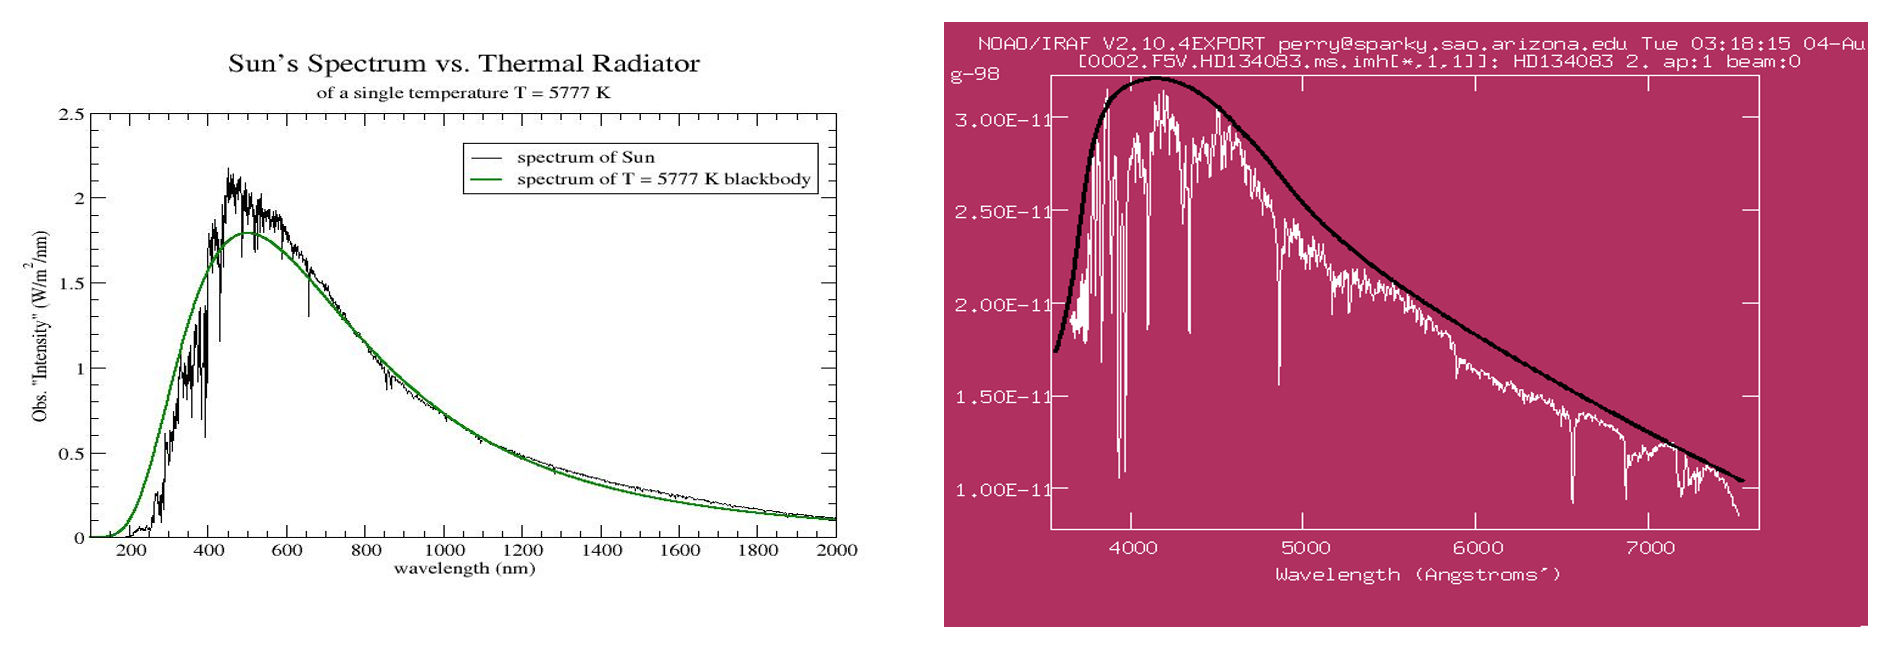
\includegraphics[width=\linewidth]{Figures/contin_spectra.png}
    \caption{\textbf{Αριστερά:} Προσαρμογή συνεχούς φάσματος θερμοκρασίας $ T \sim 5777 \ K$ στο φάσμα του Ήλιου. \textbf{Δεξιά:} Προσαρμογή συνεχούς φάσματος θερμοκρασίας $ T \sim 6660 \ K$ στο φάσμα του αστέρα HD134083. Και στις δύο περιπτώσεις είναι χαρακτηριστική η παρουσία φασματικών γραμμών απορρόφησης.}
    \label{fig:continuous_spectra}
\end{figure}

Επειδή το πλάτος $\Delta \lambda$ των φασματικών γραμμών είναι συνήθως πολύ μικρό συγκρικά με το πλάτος της οπτικής περιοχής, η φωτεινή ενέργεια που αντιστοιχεί σ' αυτές είναι πολύ μικρή, έστω κι αν η έντασή τους είναι πολύ μεγαλύτερη (ή μικρότερη) από την τιμή της συνεχούς συνιστώσας στην οπτική περιοχή. Έτσι, η ύπαρξη των φασματικών γραμμών δεν επηρεάζει σημαντικά τη φωτεινότητα ενός αστέρα και κατ' επέκταση το μέγεθός του ($m_U, m_B, m_V$ κτλ). Παρόλα αυτά, η ένταση και το πλάτος των φασματικών γραμμών των αστρικών φασμάτων είναι φορείς που μας μεταφέρουν τις σημαντικότερες πληροφορίες που έχουμε σήμερα στη διάθεσή μας για του αστέρες: φυσικές συνθήκες στην επιφάνεια και την ατμόσφαιρά τους (πίεση και θερμοκρασία), χημική σύσταση, ταχύτητα περιστροφής, ακτινική ταχύτητα ως προς τον παρατηρητή. Για παράδειγμα, η μέτρηση της μετατόπισης του μήκους κύματος των φασματικών γραμμών από τα διάφορα τμήματα της επιφάνειας του αστέρα, προς μικρότερα ή μεγαλύτερα μήκη κύματος (λόγω φαινομένου Doppler) μας επιτρέπει τη μέτρηση της ακτινικής συνιστώστας της ταχύτητας του αστέρα. Αντίστοιχα, η μέτρηση του εύρους των φασματικών γραμμών μας επιτρέπει τον προσδιορισμό της γωνιακής ταχύτητας περιστροφής του αστέρα.Γενικά πάντως, η πεπλάτυνση των φασματικών γρμαμών οφείλεται σε πολλούς παράγοντες, όπως η θερμική κίνηση των συστατικών του αερίου. Σε αυτή την περίπτωση βέβαια, η πεπλάτυνση δεν είναι ίδια για όλες τις φασματικές γραμμές που αντιστοιχούν στα διάφορα χημικά στοιχεία παρόντα στην ατμόσφαιρα του αστέρα. Η ταχύτητα περιστροφής όμως επηρεάζει το εύρος όλων των φασματικών γραμμών το ίδιο.

Η δημιουργία της συνεχούς συνιστώσας του φάσματος αν και έχει θεωρητικό ενδιαφέρον, οι ιδιότητές της λίγο εξαρτώνται από το μηχανισμό παραγωγής της και κατ' επέκταση από τη χημική σύσταση του αστέρα.

\subsection{Σχηματισμός φασματικών γραμμών}
Οι φασματικές γραμμές δημιουργούνται όταν μεταβάλλεται η ενέργεια ενός ατόμου ή ενός μορίου (ή ελεύθερης ρίζας) μεταξύ κβαντισμένων ενεργειακών σταθμών. Στην περίπτωση των μορίων, αυτό συμβαίνει είτε όταν μεταβάλλεται το πλάτος της ταλάντωσης ή η σχετική θέση των ατόμων τους, είτε όταν μεταβάλλεται η στροφορμή τους. Η ενέργεια ενός ατόμου, από την άλλη μεριά, μεταβάλλεται όταν μεταβληθεί ένας από τους τέσσερις κβαντικούς αριθμούς που χαρακτηρίζουν την ενεργειακή κατάσταση ενός ηλεκτρονίου. Η μεταβολή αυτή της ενέργειας κατά $\Delta E$ μπορεί να γίνει είτε όταν το άτομο απορροφά ($\Delta E > 0$) είτε όταν εκπέμπει $\Delta E < 0$ ένα φωτόνιο συχνότητας $\nu$, η οποία δίνεται από τη σχέση $|\Delta E| = h\nu$, όπου $h$ η σταθερά του Planck.

Όταν από μια δέσμη Η/Μ ακτινονολίας, που αποτελείται από συνεχή κατανομή συχνοτήτων, απορροφώνται φωτόνια συχνότητας $\nu_0$, τότε στο παρατηρούμενο φάσμα της δημιουργείται μία \textit{γραμμή απορρόφησης}. Όταν προστίθενται φωτόνια συχνότητας $\nu_0$, τότε στο φάσμα της επιπροστίθεται μία \textit{γραμμή εκπομπής}. Το αν η φασματική γραμμή που δημιουργείται σε κάθε περίπτωση θα είναι γραμμή εκπομπής ή απορρόφησης εξαρτάται από τη θερμοδυναμική κατάσταση της ύλης, δηλαδή των ίδιων των ατόμων.

\begin{figure}[h]
    \centering
    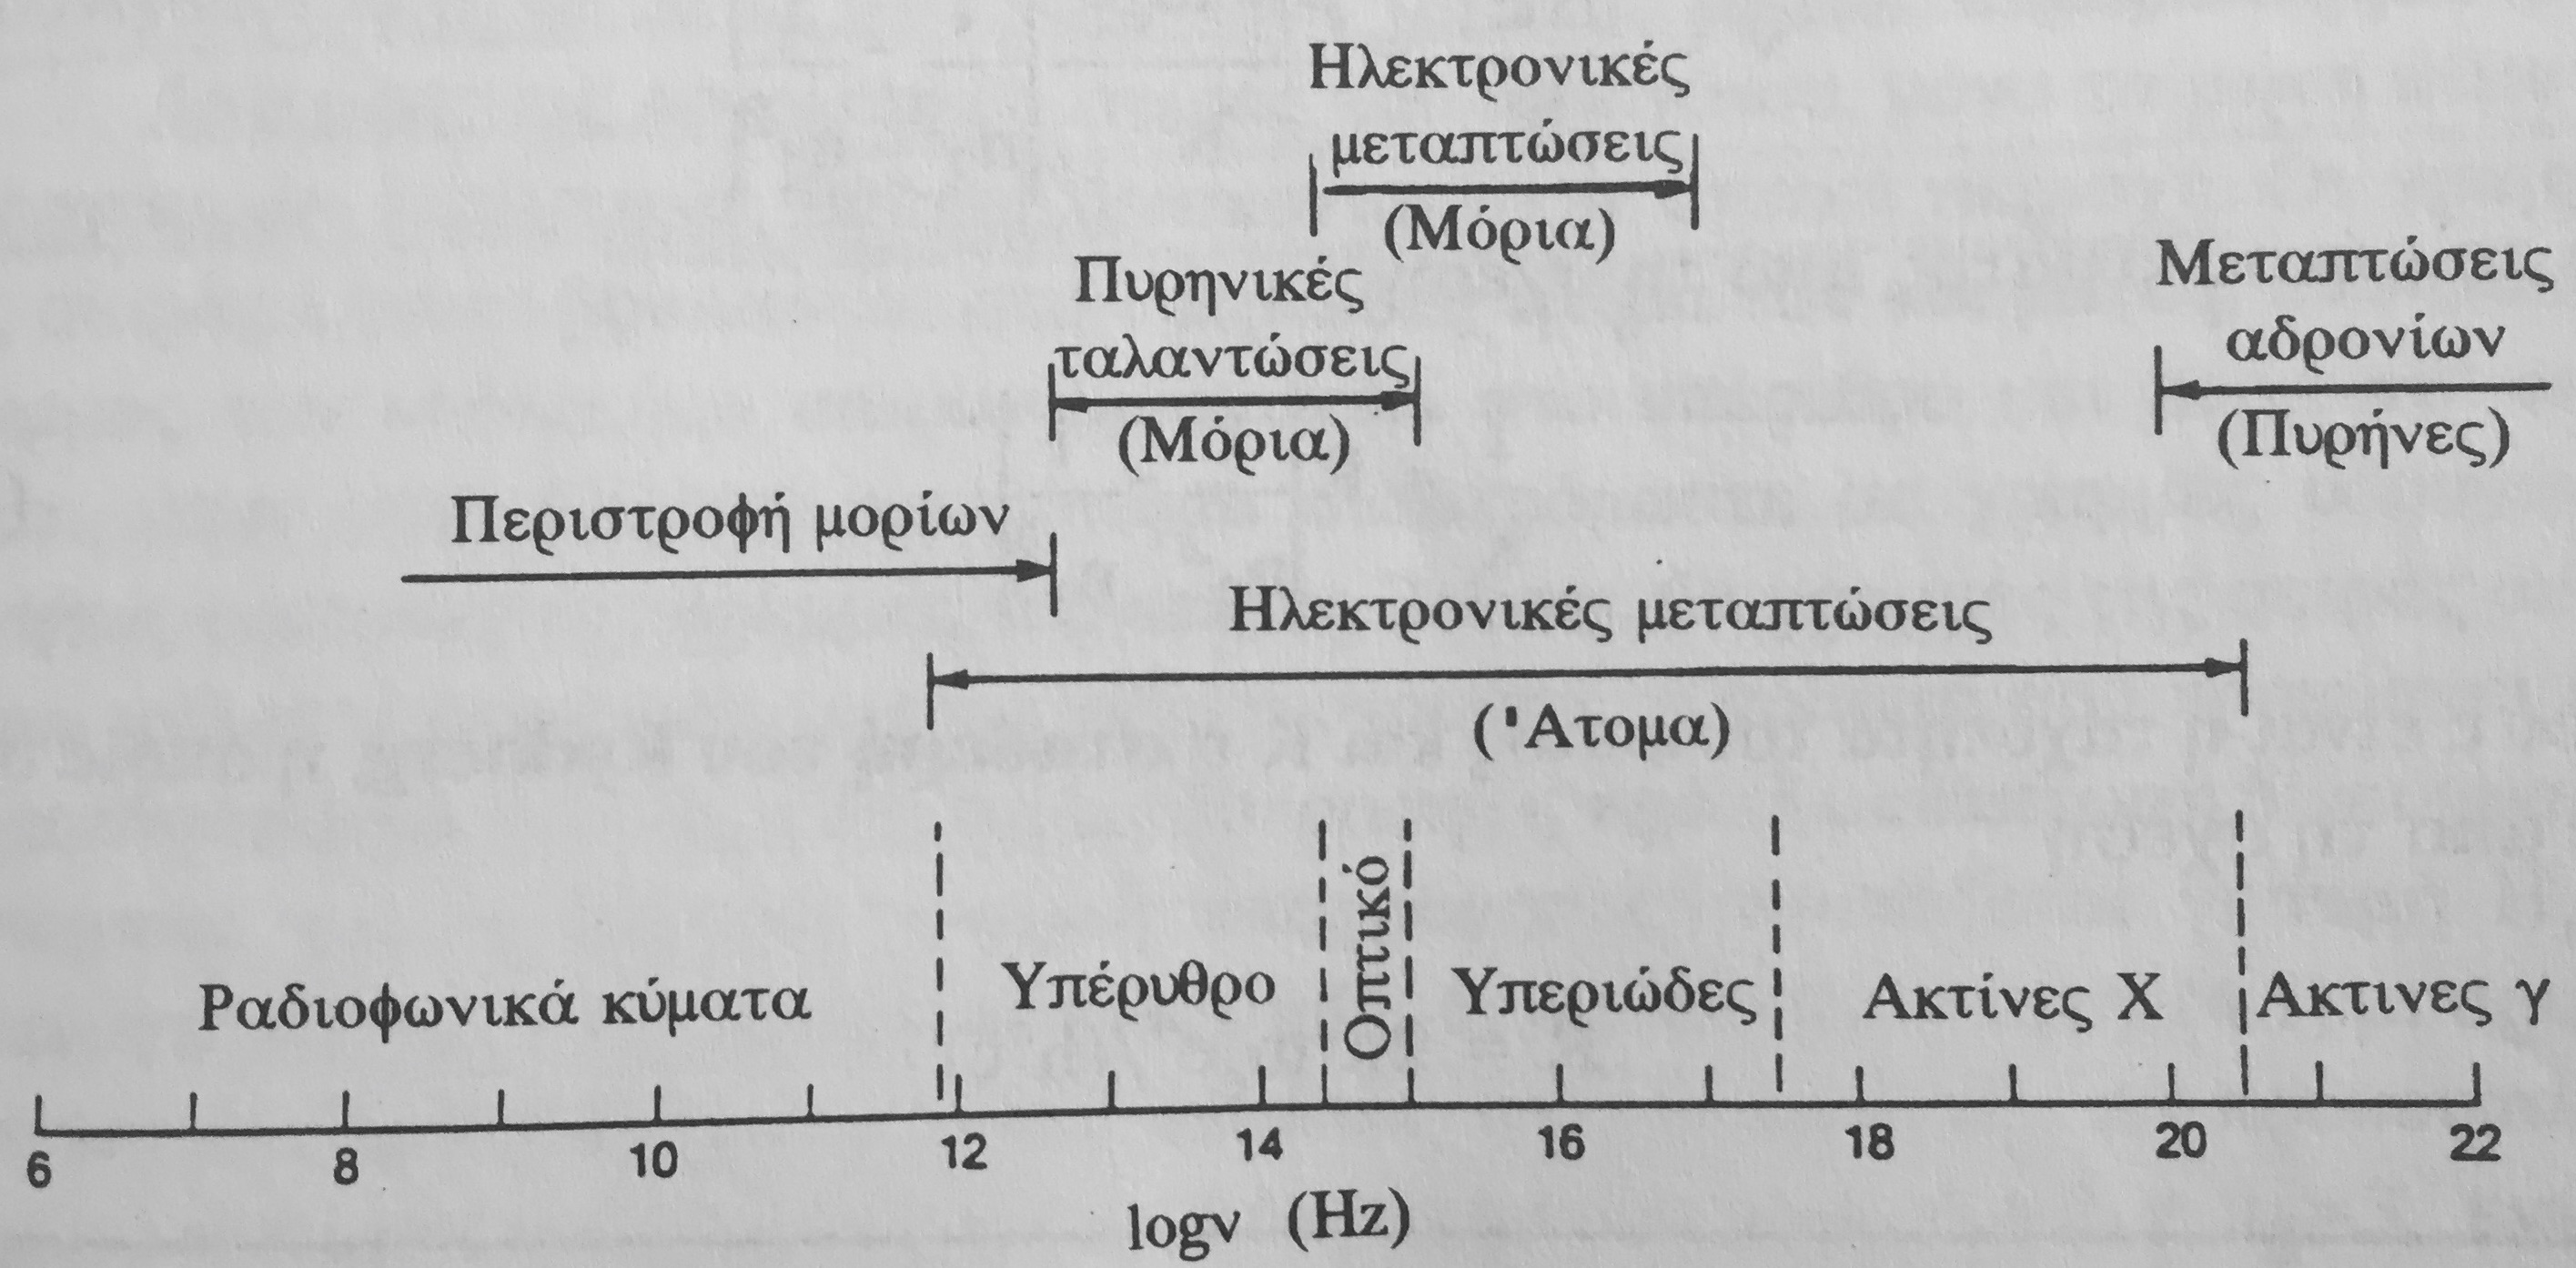
\includegraphics[width=\linewidth]{Figures/energy_transitions.jpeg}
    \caption{Ενεργειακές μεταπτώσεις στις οποίες οφείλονται η δημιουργία φασματικών γραμμών.}
    \label{fig:energy_transitions}
\end{figure}

\subsubsection{Φασματικές σειρές του Υδρογόνου}
Για λόγους απλότητας, θα θεωρήσουμε ότι η μοναδική αιτία αλλαγής της ενεργειακής κατάστασης ενός ατόμου είναι η μετάπτωση ενός ηλεκτρονίου από μία στοιβάδα σε μία άλλη, δηλαδή η αλλαγή του κύριου κβαντικού αριθμού, $(n = 1,2,3, \dots)$. Με άλλα λόγια, δεν θα μιλήσουμε καθόλου για ενεργειακές μεταπτώσεις μορίων ή ενεργειακές μεταπτώσεις υπέρλεπτης υφής (μεταπτώσεις που προκαλούνται λόγω της αλληλεπίδρασης του πυρήνα με το ηλεκτρονιακό νέφος, π.χ. γραμμή εκπομπής 21-cm του Υδρογόνου).

Το Υδρογόνο είναι με διαφορά το στοιχείο με τη μεγαλύτερη αφθονία τοσο στο σύμπαν όσο και στους αστέρες. Σε συνδυασμό με το γεγονός ότι είναι και το πιο εύκολα μελετήσιμο λόγω της απλής δομής του, τα αποτελέσματα αυτά είναι εξαιρετικά χρήσιμα.

Η ενέργεια του μοναδικού ηλεκτρονίου του ατόμου του Υδρογόνου δίνεται από τη σχέση
\begin{equation}
    E = - \frac{1}{n^2} \frac{2\pi^2 m_e e^4}{h^2}
\end{equation}
όπου $m_e$, $e$ και $n$ είναι η μάζα ηρεμίας, το φορτίο και ο κύριος κβαντικός αριθμός του ηλεκτρονίου αντίστοιχα.
Αν το ηλεκτρόνιο μεταβεί από μία στάθμη με κύριο κβαντικό αριθμό $n_i$ σε μία άλλη με κύριο κβαντικό αριθμό $n_f$, τότε η ενέργειά του μεταβάλλεται κατά 
\begin{equation}
    \Delta E = E_2 - E_1 = - \frac{2\pi^2 m_e e^4}{h^2} \left( \frac{1}{n_f^2} - \frac{1}{n_i^2} \right)
\end{equation}
Όταν $n_i < n_f$ τότε $\Delta E > 0 $, οπότε έχουμε απορρόφηση φωτονίου από το άτομο το οποίο μεταβαίνει από τη στάθμη χαμηλότερης ενέργειας ($n_i$) στη στάθμη υψηλότερης ενέργειας ($n_f$). Στην αντίθετη περίπτωση όπου $n_i > n_f$, έχουμε εκπομπή φωτονίου. Και στις δύο περιπτώσεις, η συχνότητα του φωτονίου δίνεται από τη σχέση

\begin{equation}
    \nu = \frac{|\Delta E|}{h} = \frac{2 \pi^2 m_e e^4}{h^3} \left| \frac{1}{n_f^2} - \frac{1}{n_i^2} \right|
\end{equation}
και το μήκος κύματος από τη σχέση του Rydberg

\begin{equation}
    \label{eq:rydberg_formula}
    \frac{1}{\lambda} = Z^2 R \left| \frac{1}{n_f^2} - \frac{1}{n_i^2} \right|
\end{equation}
όπου $Z$ είναι ο ατομικός αριθμός του ατόμου και $R$ η σταθερά του Rydberg η οποία δίνεται από τη σχέση $$R = \frac{2\pi^2 m_e e^4}{h^3 c}$$

Εφαρμόζοντας τη σχέση \eqref{eq:rydberg_formula} για το άτομο του Υδρογόνου ($Z=1$) τότε προκύπτουν οι εξής σειρές (δες και σχήμα \ref{fig:hydrogen_lines}):

\begin{itemize}
    \item Για $n_f = 1$ και $n_i=2,3, \dots$ τότε έχουμε τη σειρά \textit{εκπομπής Lyman}. Στην περίπτωση που $n_i = 1$ και $n_f = 2,3, \dots$ τότε έχουμε τη σειρά \textit{απορρόφησης Lyman}.
    \item Για $n_f = 2$ και $n_i=3,4, \dots$ τότε έχουμε τη σειρά εκπομπής Balmer. Στην περίπτωση που $n_i = 2$ και $n_f = 3,4, \dots$ τότε έχουμε τη σειρά απορρόφησης Balmer. Αυτή η σειρά είναι και η πιο σημαντική στην Οπτική Αστρονομία καθώς τα μήκη κύματος αυτής της σειράς βρίσκονται στην οπτική περιοχή. 
    
    Η γραμμή που προκύπτει από την μετάπτωση $n_i = 3 \rightarrow n_f = 2$ ονομάζεται γραμμή εκπομπής $H_{\alpha}$. Αντίστοιχα, η αντίστροφη μετάβαση $n_i = 2 \rightarrow n_f = 3$ ονομάζεται γραμμή απορρόφησης $H_{\alpha}$. Με την ίδια λογική μπορούμε να ορίσουμε τη γραμμή Balmer $H_{\beta}$ που αντιστοιχεί στην μετάβαση $n_i = 4 \rightarrow n_f = 2$ (ή το αντίστροφο), την γραμμή $H_{\gamma}$ για την μετάβαση $n_i = 5 \rightarrow n_f = 2$ κτλ.
    
    Το μήκος κύματος της σειρά Balmer ξεκινάει από $\lambda(H_{\alpha}) = 6563$Å και μειώνεται όσο αυξάνει η τάξη της γραμμής τείνοντας σε μια οριακή τιμή $\lambda(H_{\infty}) = 3546$Å. Στην περιοχή του οριακού αυτού μήκους κύματος οι γραμμές απορρόφησης είναι τόσο κοντά η μία με την άλλη, ώστε αλληλοεπικαλύπτονται με αποτέλεσμα το υπόβαθρο στην περιοχή αυτή να εμφανίζει μία ασυνέχεια, η οποία ονομάζεται \textbf{ασυνέχεια Balmer} και το ύψος της εξαρτάται από τη θερμοκρασία του αστέρα προσφέροντας έτσι ένα ακόμα παρατηρησιακό εργαλείο για τη μέτρησή της. 
    \item Για $n_f = 3$ και $n_i=4,5, \dots$ τότε έχουμε τη σειρά \textit{εκπομπής Paschen} (και αντίστροφα για την γραμμή απορρόφησης).
    \item Για $n_f = 4$ και $n_i=5,6, \dots$ τότε έχουμε τη σειρά \textit{εκπομπής Brackett} (και αντίστροφα για την γραμμή απορρόφησης).
    \item Για $n_f = 5$ και $n_i=6,7, \dots$ τότε έχουμε τη σειρά \textit{εκπομπής Pfund} (και αντίστροφα για την γραμμή απορρόφησης).
    \item Για $n_f = 6$ και $n_i=7,8, \dots$ τότε οι σειρές που προκύπτουν δεν έχουν κάποια συγκεκριμένη ονομασία.
\end{itemize}


\begin{figure}[h]
    \centering
    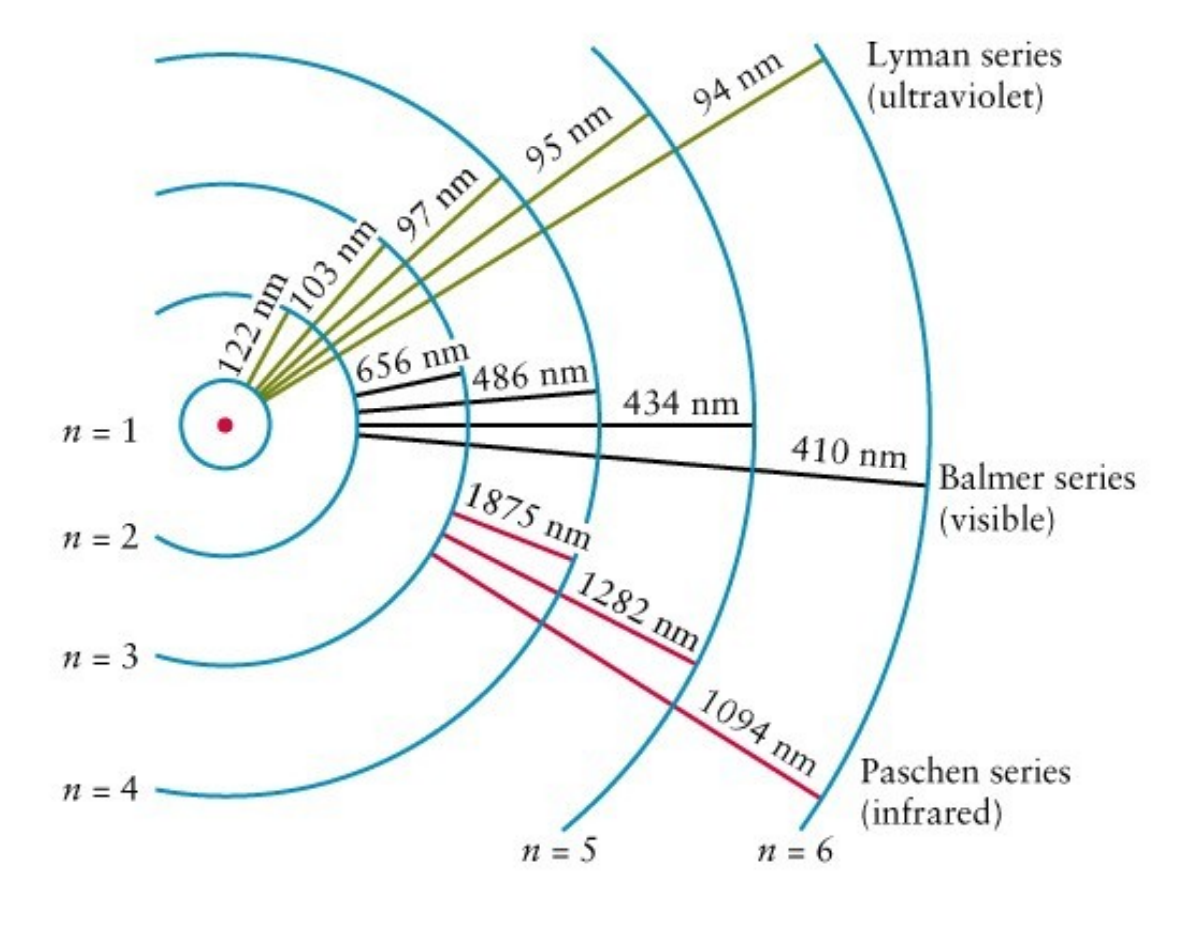
\includegraphics[scale=0.5]{Figures/hydrogen_spectral_lines.png}
    \caption{Σειρές Lyman, Balmer και Paschen για το άτομο του Υδρογόνου. Οι σειρές Brackett και Pfund, καθώς και άλλες ανώτερες σειρές, δεν παρουσιάζονται στο συγκεκριμένο διάγραμμα.}
    \label{fig:hydrogen_lines}
\end{figure}



\subsection{Φαινόμενο Zeeman}
Όταν τα άτομα στα οποία οφείλεται η δημιιουργία των φασματικών γραμμών βρίσκονται σε μαγνητικό πεδίο, τότε οι ενεργειακές τους στάθμες μεταβάλλονται, έτσι ώστε κάθε φασματική γραμμή διασπάται σε δύο, ή περισσότερες, πολωμένες συνιστώσες. Το φαινόμενο αυτό ονομάζεται ``φαινόμενο Zeeman'' (το ηλεκτρικό ανάλογο αυτού του φαινομένου είναι το φαινόμενο Stark όπου οι φασματικές γραμμές διασπόνται υπό την παρουσία ηλεκτρικού πεδίου) και επειδή η απόσταση των διάφορων συνιστωσών εξαρτάται από την ένταση του μαγνητικού πεδίου, το εκμεταλλευόμαστε για την μέτρηση αστρικών, μεσοαστρικών και γαλαξιακών μαγνητικών πεδίων. 

Στην απλούστερη περίπτωση (το ομαλό φαινόμενο Zeeman) μία φασματική γραμμή συχνότητας $\nu_{\circ}$ διασπάται σε τρεις συνιστώσες με συχνότητες $\nu_{\circ} - \Delta \nu$, $\nu_{\circ}$, και $\nu_{\circ} + \Delta \nu$. Αν η ένταση του μαγνητικού πεδίου, $B$, μετριέται σε Gauss, τότε η διαφορά συχνότητας $\Delta \lambda$, δίνεται απο τη σχέση 
\begin{equation}
    \Delta \nu =  \frac{eB}{4\pi m c} = 1.4 \times 10^6 \ B \ \ Hz
\end{equation}

Οι συσκευές μέτρησης των μαγνητικών πεδίων που βασίζονται σε παρατηρήσεις Η/Μ ακτινοβολίας ονομάζονται \textit{μαγνητογράφοι}. 



\section{Φασματική Ταξινόμηση}
Όπως είδαμε, Οι παράγοντες που καθορίζουν το φάσμα ενός αστέρα είναι η επιφανειακή θερμοκρασία ($ T_{eff}$), η ταχύτητα του αστέρα ($\boldsymbol{u}$), η γωνιακή ταχύτητα περιστροφής ($\boldsymbol{\omega}$), η ένταση του μαγνητικού πεδίου ($\boldsymbol{B}$), και η πίεση στην επιφάνεια του αστέρα. Τα αστρικά αυτά φάσματα κυριαρχούνται από γραμμές απορρόφησης (ορισμένα άστρα εμφανίζουν και αδύναμες γραμμές εκπομπής) με τις συνηθέστερες γραμμές απορρόφησης να είναι αυτές της σειράς Balmer του Υδρογόνου. Επειδή η ένταση των γραμμών απορρόφησης εξαρτάται άμεσα από την ενεργό θερμοκρασία του αστέρα, μπορούμε να ταξινομήσουμε τα αστέρια με βάση την ένταση των γραμμών απορρόφησης του Υδρογόνου και να καθορίσουμε με αυτό τον τρόπο την ενεργό θερμοκρασία τους.



\subsection{Ταξινόμηση κατα Harvard}
Αρχικά οι αστρονόμοι ταξινόμησαν τα αστρικά φάσματα αλφαβητικά σε φασματικούς τύπους (spectral types, Sp) με πρώτο κριτήριο την ένταση της γραμμής $H_{\alpha}$ της σειράς Balmer. Έτσι τα αστέρια τύπου Α είχαν την εντονότερη γραμμή $H_{\alpha}$, οι τύπου Β αστέρες είχαν λιγότερο έντονη γραμμή $H_{\alpha}$ κ.ο.κ.
Για τους αστέρες που είχαν τόσο ασθενή γραμμή $H_{\alpha}$, ώστε να μην μπορεί να χρησιμοποιηθεί ως κριτήριο ταξινόμησης, οι αστρονόμοι εισήγαγαν ως συμπληρωματικά κριτήρια την παρουσία ή την απουσία και άλλων φασματικών γραμμών (π.χ. ουδέτερα άτομα, ιόντα, μοριακές ταινίες).

Με την ανάλυση πολλών φασμάτων, διαπιστώθηκε ότι οι γραμμές απορρόφησης -εκτός του Υδρογόνου- δεν έδειχναν να μεταβάλλονται ομαλά από τον έναν φασματικό τύπο στον επόμενο. Αντίθετα, έδειχναν να εμφανίζονται και να εξαφανίζονται απότομα. Έτσι, οδηγήθηκαν στην αναδιάταξη της -αρχικά αλφαβητικής- ακολουθίας των φασματικών τύπων σε μία νέα ακολουθία όπου το χαρακτηριστικό της ήταν η συνεχής και μονότονη μεταβολή της ενεργού θερμοκρασίας. Η φασματική ταξινόμηση που προέκυψε ονομάστηκε ταξινόμηση κατα Harvard (σχήμα \ref{fig:spectral_classes_harvard}) επειδή προτάθηκε από ερευνητές του Πανεπιστημίου του Harvard.

Κάθε φασματικός τύπος της συγκεκριμένης ταξινόμησης διαιρείται σε δέκα υποκατηγορίες που χαρακτηριζόνται από τους αριθμούς $0,1,2,\dots , 9$. Ένα αστέρι φασματικού τύπου $ F1$ είναι πιο θερμό από ένα αστέρι $ F3$ αλλά πιο ψυχρό από ένα αστέρι $ A9$. Έτσι, οι θερμότεροι αστέρες που έχουν παρατηρηθεί μέχρι σήμερα είναι αστέρες φασματικού τύπου $ O5$ $ T_{eff} = 50000 \ K$, ενώ οι ψυχρότεροι αστέρες (ερυθροί νάνοι) είναι φασματικού τύπου $ M9$ με $ T_{eff} = 2900 \ K$. Ένας γενικός μνημονικός κανόνας για την συγκεκριμένη ταξινόμηση είναι 
\begin{center}
    \textbf{O}h, \textbf{B}e \textbf{A} \textbf{F}ine \textbf{G}irl/\textbf{G}uy, \textbf{K}iss \textbf{M}e
\end{center}


\begin{figure}[h]
    \centering
    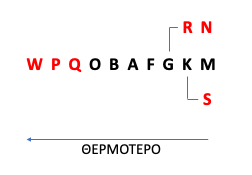
\includegraphics[scale=0.6]{Figures/spectral_classes.png}
    \caption{Φασματική ταξινόμηση κατά Harvard βάσει την ενεργό θερμοκρασία των άστρων. Κάθε τύπος αποτελείται από 10 υποκατηγορίες από το 0 εώς το 9. Οι τύποι P και Q δεν είναι απαραίτητο να ακολουθούν την μονότονη αύξηση της επιφανειακής θερμοκρασίας βάσει της οποίας ταξινομούνται τα αστέρια στους υπόλοιπους τύπους.}
    \label{fig:spectral_classes_harvard}
\end{figure}

Όπως φαίνεται και στο σχήμα \ref{fig:spectra_comparisson_table}, η ένταση των γραμμών Balmer ξεκινάει σχεδόν από το μηδεν ($ Sp = O5$), φτάνει σε κάποιο μέγιστο ($ Sp = A$) και καταλήγει πάλι κοντά στο μηδέν ($ Sp = M$). Αυτό συμβαίνει γιατί σε αστέρια με πολύ υψηλές θερμοκρασίες ($ > 10000 \ K$) το άτομο του Υδρογόνου έχει χάσει το μοναδικό του ηλεκτρόνιο και άρα δεν μπορεί να δώσει μετάπτωση. Τα φάσματα τέτοιων θερμών αστέρων θα περιέχουν ιόντα από σχετικά απλά άτομα που χρειάζονται πολύ ενέργεια για να διώξουν τα εξωτερικά τους ηλεκτρόνια σε σύγκριση με πιο βαριά άτομα που τα εξωτερικά τους ηλεκτρόνια είναι πιο ``χαλαρά'' δεμένα με το δυναμικό του πυρήνα.
Στην αντίθετη περίπτωση που το άστρο είναι πολύ ψυχρό, το ηλεκτρόνιο βρίσκεται στη βασική του στοιβάδα οπότε πάλι δεν μπορεί να δώσει την μετάπτωση που απαιτείται για τις γραμμές Balmer. Η χαμηλή θερμοκρασία εξηγεί και την ύπαρξη μοριακών ταινιών στα φάσματα αυτών των αστέρων.\\

{\color{red} \hrule}
\textbf{Ερμηνεία της κατάταξης κατά Harvard}\\
Η φασματική ακολουθία $ O, B, \dots, M$ είναι στην πραγματικότητα μία μονότονη και φθίνουσα συνάρτηση της θερμοκρασίας. Καθώς η θερμοκρασία ελλατώνεται βαθμιαία από τους αστέρες τύπου Ο προς τους αστέρες τύπου Μ, η αριθμητική πυκνότητα των ιονισμένων ατόμων ελλατώνεται, ενώ αυξάνεται η αριθμητική πυκνότητα των ουδέτερων ατόμων. Έτσι, οι γραμμές των ιονισμένων ατόμων που κυριαρχούν στους αστέρες τύπου Ο, παραχωρούν τη θέση τους στις γραμμές των ουδέτερων ατόμων, και τελικά στις μοριακές ταινίες. Η ερμηνεία αυτή βασίζεται στον νόμο του Saha.\\
{\color{red} \hrule}

\begin{figure}[h]
   \centering
\begin{subfigure}[h]{0.45\textwidth}
	\centering
   	 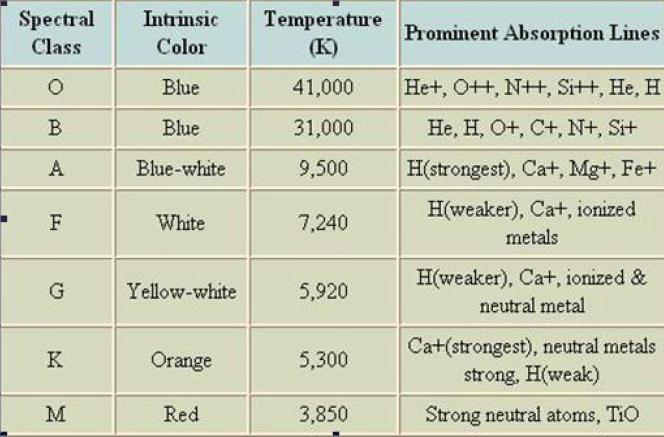
\includegraphics[angle=270,width=\textwidth]{Figures/spectral_class_table.png} 
\end{subfigure}
\begin{subfigure}[h]{0.5\textwidth}
	\centering
	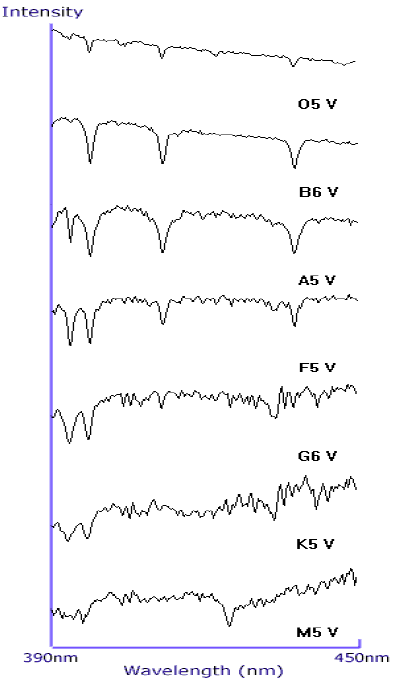
\includegraphics[scale=0.5]{Figures/spectra_comparison_harvard.png} 
    \end{subfigure}
    \caption{\textbf{Αριστερά}: Πίνακας με στοιχεία για κάθε φασματικό τύπο. \textbf{Δεξιά}: Σύγκριση φασμάτων αστέρων της κύριας ακολουθίας.}
    \label{fig:spectra_comparisson_table}
\end{figure}

Οι έξι συμπληρωματικοί φασματικοί τύποι (κόκκινα γράμματα στο σχήμα \ref{fig:spectral_classes_harvard}) περιγρέφουν μη-συνηθισμένους αστέρες. Ο τύπος W χαρακτηρίζει αστέρες τύπου \textbf{Wolf-Rayet} οι οποίοι είναι όμοιοι με αυτούς του τύπου Ο, αλλά με ευρείες γραμμές εκπομπής, οι οποίες οφείλονται σε ανώμαλα εκτεταμένη ατμόσφαιρα.
Ο τύπος P χαρακτηρίζει \textbf{πλανητικά νεφελώματα}, ένα από τα τελικά στάδια της εξέλιξης ενός αστέρα μικρής μάζας, τα οποία αποτελούνται από εξαιρετικά αραιό αέριο και σκόνη.
Ο τύπος Q ορίστηκε για την περιγραφή των φασμάτων \textbf{καινοφανών αστέρων} (novae), αστέρες που εμφανίζουν ξαφνική αύξηση της φωτεινότητάς τους κατά πολλά μεγέθη λόγω εκρηκτικής ανάφλεξης πυρηνικού καυσίμου. Αυτό μπορεί να συμβεί είτε σε διπλό σύστημα λόγω μεταφοράς μάζας από τον ένα αστέρα στον άλλον (δες Κεφάλαιο \ref{ch:Chapter7}), είτε και σε απλούς αστέρες όταν διάφοροι μηχανισμοί πρόσμιξης μεταφέρουν φρέσκο υλικό από ανώτερα στρώματα, στα στρώματα που γίνεται καύση βαρύτερων υλικών. Πάντως ο φασματικός τύπος Q χρησιμοποιείται σπάνια σήμερα.
Τέλος, οι αστέρες φασματικού τύπου R, N και S έχουν ανώμαλη χημική σύσταση, με τα φάσματα των αστέρων R και N να περιέχουν ασυνήθιστα υψηλή περιεκτικότητα σε άνθρακα (μοριακές ταινίες της ελεύθερης ρίζας CH και CN αντίστοιχα) και να ονομάζονται \textbf{αστέρες άνθρακα}. Από την άλλη, τα αστέρια φασματικού τύπου S, έχουν έντονες μοριακές ταινίες των οξειδίων του τιτανίου, ζιρκονίου και άλλων σπάνιων γαιών. Αυτη η ανώμαλη χημική σύσταση αυτών των αστέρων μάλλον οφείλεται σε κάποιον μιχανσιμό ανάμιξης της επιφανειακής ύλης με ύλη που προέρχεται από το εσωτερικό του αστέρα μέσω ρευμάτων μεταφοράς. 
Ας σημειωθεί εδώ ότι οι έξι αυτοί φασματικοί τύποι που αναλύσαμε δεν αποτελούν γνήσια επέκταση της αρχικής φασματικής ταξινόμησης, καθώς δεν παρουσιάζουν αμφιμονοσήμαντη αντιστοιχία μεταξύ των φασματικών τύπων και των ενεργών θερμοκρασιών. Τα αστέρια που ανήκουν σε αυτές ή αλλες φασματικές κατηγορίες που δεν εμφανίζονται εδώ (π.χ. L και T κατηγορίας καφέ νάνων) αποτελούν πολύ μικρό ποσοτό της τάξης $< 1 \%$.

Παρόλα αυτά, υπάρχουν αστέρια που φυσικά η ενεργός τους θερμοκρασία εμπίπτει στα όρια $ 3000 - 50000 \ K$ αλλά το φάσμα τους δεν ταιριάζει με κανέναν από τους παραπάνω φασματικούς τύπους. Γι' αυτό γενικά η χρήση της θερμοκρασίας ή του δείκτη χρώματος (που είναι συνάρτηση της θερμοκρασίας) προτιμάται έναντι του φασματικού τύπου.



\subsection{Διάγραμμα Hertzsprung-Russell}
Αν τοποθετήσουμε τους αστέρες με γνωστά φάσματα σε ένα δισδιάστατο διάγραμμα που έχει τετμημένη τον φασματικό τύπο (Sp) και τεταγμένη το απόλυτο μέγεθος του αστέρα, τότε παρατηρούμε ότι οι αστέρες δεν είναι τυχαία διασκορπισμένοι στο επίπεδο, αλλά συγκεντρώνονται σε συγκεκριμένες δομές. Το διάγραμμα αυτό ονομάζεται \textbf{διάγραμμα Hertzprung-Russel} ή για συντομία διάγραμμα H-R.
Η μορφή του διαγράμματος H-R μας δείχνει ότι υπάρχουν φυσικοί νόμοι που συνδέεουν τη λαμπρότητα του αστέρα (απόλυτο μέγεθος) με την ενεργό θερμοκρασία του (φασματικό τύπο) και ότι όλα τα βασικά παρατηρησιακά μεγέθη ενός αστέρα δεν έχουν τυχαίες τιμές, αλλά συνδέονται με σχέσεις που μπορούν να εξηγηθούν και θεωρητικά. Φυσικά μία σχέση της μορφής $$ L = f(T_{eff})$$ που αποκαλύπτει το διάγραμμα H-R είναι προσεγγιστική καθώς οι αστέρες χαρακτηρίζονται και από άλλες ποσότητες, όπως η χημική σύσταση, που σε πρώτη φάση αγνοούνται. Γι' αυτό άλλωστε και οι αστέρες δεν βρίσκονται στο διάγραμμα H-R κατά μήκος μονοδιάστατων καμπυλών, αλλά παρουσιάζουν μία κάποια διασπορά.

\begin{figure}[h]
    \centering
    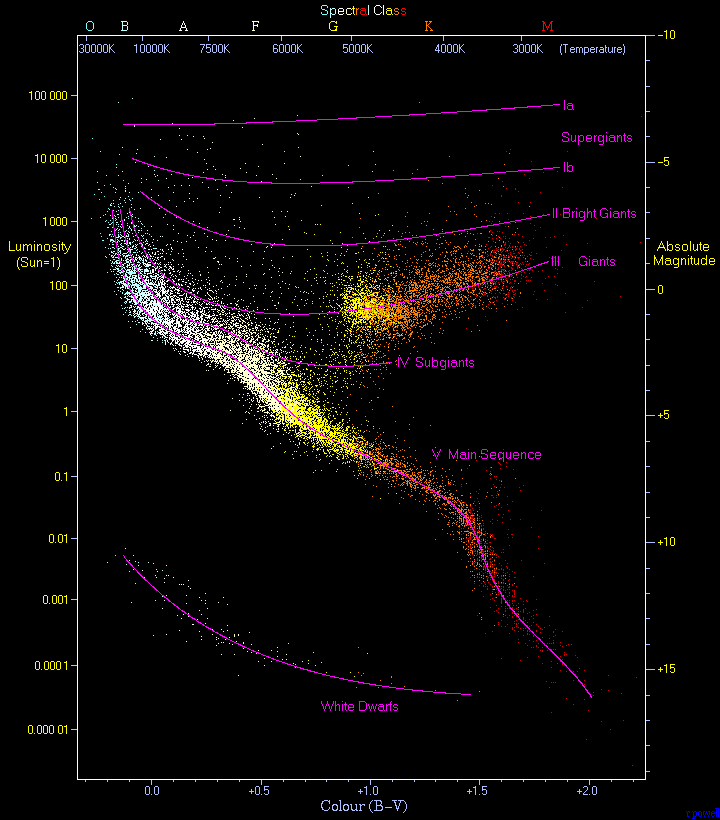
\includegraphics[scale=0.4]{Figures/HRDiagram.png}
    \caption{Διάγραμμα Hertzprung-Russel.}
    \label{fig:HRD}
\end{figure}

Από το σχήμα \ref{fig:HRD} παρατηρούμε ότι τα περισσότερα αστέρια είναι συγκεντρωμένα σε μία ζώνη, που διατρέχει το διάγραμμα διαγώνια και η οποία ονομάζεται \textbf{κύρια ακολουθία}. Πάνω από την κύρια ακολουθία υπάρχει μία άλλη ζώνη αστέρων, που ονομάζεται \textbf{κλάδος γιγάντων}. Τέλος, κάτω από τον κλάδο της κύριας ακολουθίας υπάρχει μία συγκέντρωση αστέρων, που βρίσκεται αριστερά του διαγράμματος και σε αυτή ανήκουν οι \textbf{λευκοί νάνοι}. Αν προεκτείνουμε την γραμμή του κλάδου των γιγάντων προς τα αριστερά, παρατηρούμε ότι τέμνει την κύρια ακολουθία σ' ένα σημείο που αντιστοιχεί περίπου στον φασματικό τύπο A0 και απόλυτο μέγεθος $ M = +1$. Οι αστέρες που βρίσκονται αριστερά από το φασματικό τύπο Α0 ονομάζονται αστέρες \textbf{προγενέστερου φασματικού τύπου} (π.χ. κυανοί γίγαντες), ενώ οι αστέρες που βρίσκονται δεξιά από τον φασματικό τύπο Α0 ονομάζονται αστέρες \textbf{μεταγενέστερου φασματικού τύπου} (π.χ. ερυθροί νάνοι, νάνοι της κύριας ακολουθίας κτλ). Οι αστέρες μεταγενέστερου φασματικού τύπου που βρίσκονται πάνω από την κύρια ακολουθία ονομάζονται \textbf{ερυθροί γίγαντες}. Η διάκριση των αστέρων σε αστέρες προγενέστερου και μεταγενέστερου φασματικού τύπου δεν έχει σήμερα καμία άλλη σημασία παρά μόνο την περιγραφή της θέσης τους στο διάγραμμα H-R. Αντίθετα, η διάκριση των αστέρων σε νάνους και γίγαντες έχει φυσική σημασία.

\textbf{Αστρικά σμήνη}\\
Μπορούμε να διακρίνουμε δύο ειδών αστρικών σμηνών. Τα \textbf{σφαιρωτά σμήνη} είναι πυκνές συγκεντρώσεις μεγάλου αριθμού αστέρων ($10^4 - 10^6$) με σφαιρικό σχήμα, που κινούνται σε ελειπτικές τροχιές στην άλω γύρω από το κέντρου του Γαλαξία. Το χαρακτηριστικό των σφαιρωτών σμηνών είναι ότι επειδή σχηματίστηκαν από την βαρυτική κατάρρευση του ίδιου μοριακού νέφους, αποτελούνται σε πρώτη προσέγγιση από άστρα της ίδιας χημικής σύστασης (ίδια ``μεταλλικότητα''), της ίδιας ηλικίας, και βρίσκονται στην ίδια απόσταση από τη Γη.
Η άλλη κατηγορία αστρικών σμηνών είναι τα \textbf{ανοικτά σμήνη} τα οποία είναι συγκεντρώσεις το πολύ μερικών χιλιάδων άστρων που σχηματίστηκαν και αυτά από το ίδιο μοριακό νέφος, αλλά τα αστέρια είναι πληθυσμού I, και άρα πολύ νεώτερα συγκριτικά με τα αστέρια στα σφαιρωτά σμήνη που είναι πληθυσμού ΙΙ. Τα ανοικτά σμήνη βρίσκονται κυρίως στο Γαλαξιακό επίπεδο και όχι στην άλω.


\begin{figure}[h]
    \centering
    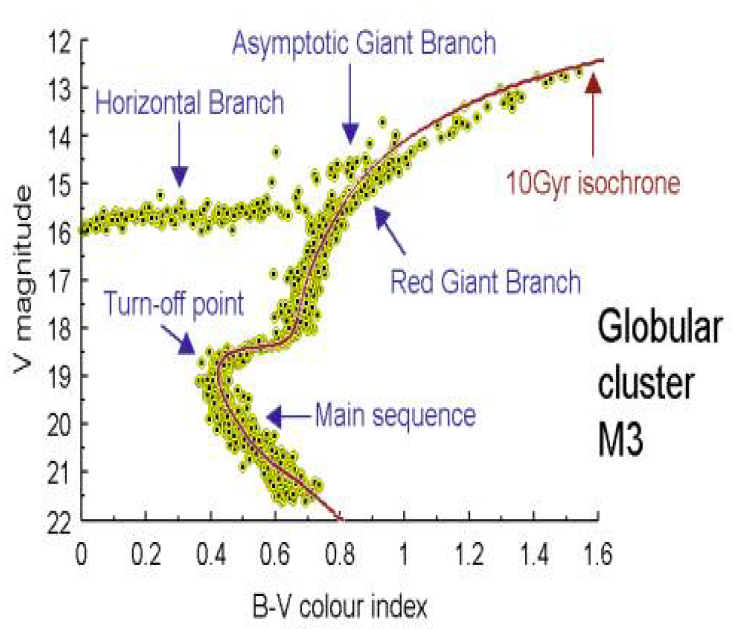
\includegraphics[scale=0.4]{Figures/cmd.png}
    \caption{Διάγραμμα Χρώματος-Μεγέθους για το σφαιρωτό σμηνος Μ3. Στο διάγραμμα φαίνεται μια ισόχρονη καμπύλη των 10Gyr.}
    \label{fig:CMD}
\end{figure}

Είναι προφανές ότι δεν μπορούμε να πάρουμε το φάσμα για κάθε ένα από τα αστέρια-μέλη ενός σμήνους. Γι' αυτό το λόγο, όταν θέλουμε να κάνουμε το διάγραμμα H-R στην περίπτωση σμήνους αστέρων, εκφράζουμε την τετμημένη σε όρους δείκτη χρώματος (που είναι συνάρτηση της θερμοκρασίας και μπορεί να υπολογιστεί για χιλιάδες αστέρια που βρίσκονται στο ίδιο οπτικό πεδίο) αντί για φασματικό τύπο, και την τεταγμένη σε μέγεθος αντί για λαμπρότητα. Έτσι προκύπτει το λεγόμενο \textbf{διάγραμμα χρώματος-μεγέθους} (color-magnitude diagram) που φαίνεται στο σχήμα \ref{fig:CMD}.

Αν η συνάρτηση αρχικής μάζας (initial mass funtion) ενός σμήνους είναι γνωστή, τότε μπορούμε να υπολογίσουμε θεωρητικά μια ισόχρονη καμπύλη για οποιαδήποτε ηλικία θέλουμε, με το να προσομειώσουμε την εξέλιξη του κάθε αστέρα του αστρικού πληθυσμού και κάνοντας το διάγραμμα H-R για αυτά τα αστέρια. Συγκρίνοντας τις θεωρητικές αυτές καμπύλες που αντιστοιχούν σε συγκεκριμένες ηλικίες με το παρατηρησιακό διάγραμμα χρώματος-μεγέθους, μπορούμε να έχουμε μία εκτίμηση για την ηλικία του σμήνους.





\subsection{Ταξινόμηση κατα Yerkes}
Αστέρια ίδιου φασματικού τύπου (ίδιας ενεργού θερμοκρασίας) εμφανίζουν κατανομή στις λαμπρότητές τους, όπως φαίνεται και από το διάγραμμα H-R (σχήμα \ref{fig:HRD}). Για παράδειγμα, ο εγγύτατος του Κενταύρου έχει την ίδια επιφανειακή θερμόκαρσία με αυτή του Betelgeuse, άρα ανήκουν στον ίδιο φασματικό τύπο, αλλά τελείως διαφορετικές λαμπρότητες με τον εγγύτατο να έχει 100 φορές μικρότερη λαμπρότητα από τον Ήλιο και τον Betelgeuse 100,000 φορές μεγαλύτερη λαμπρότητα.

Το 1930, οι Morgan \& Keenan, πρότειναν ένα νέο σύστημα ταξινόμησης των αστέρων, το οποίο λειτουργεί συμπληρωματικά του συστήματος ταξινόμησης κατα Harvard. Το νέο σύστημα βασίζεται στην έννοια της \textit{Κατηγορίας λαμπρότητας}. Σύμφωνα με αυτή την ταξινόμηση, αστέρια της \textbf{ίδιας} ενεργούς θερμοκρασίας (ίδια φασματική τάξη), χωρίζονται σε έξι κατηγορίες λαμπρότητας, με βάση το \textbf{πλάτος} των γραμμών απορρόφησης (σχήμα \ref{fig:spectral_classes_yerkes}).

\begin{figure}[h]
   \centering
\begin{subfigure}[h]{0.42\textwidth}
	\centering
   	 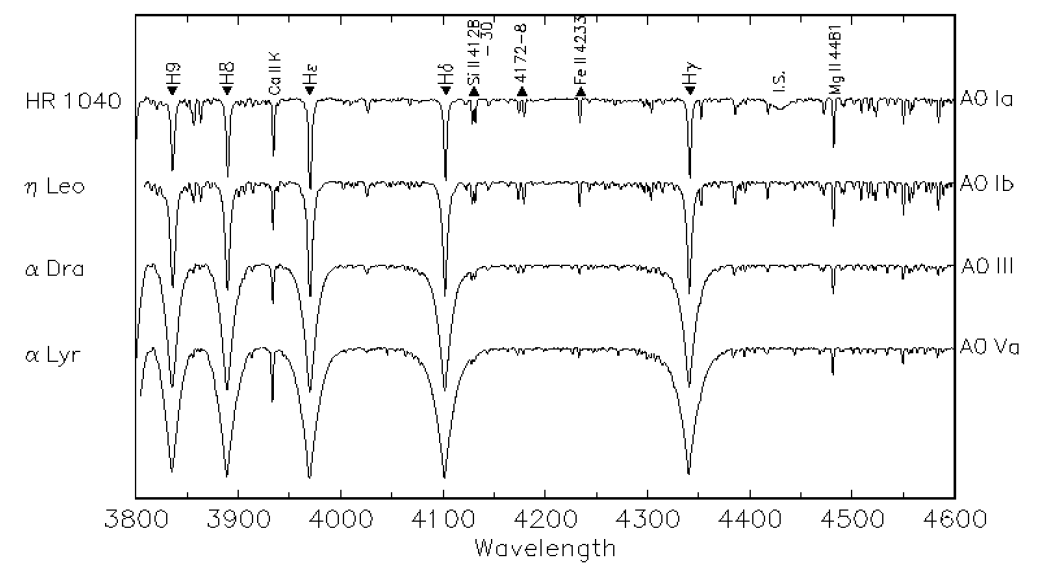
\includegraphics[angle=270,origin=c,scale=0.3]{Figures/luminosity_variations_yerkes.png} 
\end{subfigure}
\begin{subfigure}[h]{0.55\textwidth}
	\centering
	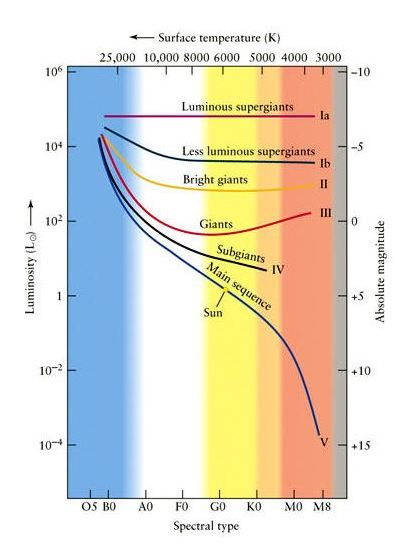
\includegraphics[scale=0.6]{Figures/spectral_classes_yerkes.jpg} 
    \end{subfigure}
    \caption{\textbf{Αριστερά}: Διακύμανση του πλάτους των γραμμών απορρόφησης για τέσσερια αστέρια φασματικού τύπου Α0 (HR 1040, $\eta$ Leo, $\alpha$ Dra, $\alpha$ Lyr). \textbf{Δεξιά}: Φασματική ταξινόμηση κατά Yerkes, σε έξι κατηγορίες λαμπρότητας. Για μεγαλύτερη κατηγορία λαμπρότητας ($ I, II, \dots VI$) το πλάτος της γραμμής απορρόφησης αυξάνεται, ενώ η ακτίνα και η λαμπρότητα μειώνονται. Ο Ήλιος ανήκει στην κατηγόρια G2V.}
    \label{fig:spectral_classes_yerkes}
\end{figure}

\vspace{0.5cm}
{\color{red} \hrule}
\textbf{Ερμηνεία της κατάταξης κατά Yerkes}\\
Εφόσον μιλάμε για αστέρια ίδιου φασματικού τύπου, το εύρος της γραμμής απορρόφησης δεν οφείλεται σε διαφορές στην ενεργό θερμοκρασία (ούτε στην περιστροφή των αστέρων) αλλά στην πίεση στην επιφάνεια των αστέρων. Κάνοντας μερικές απλές παραδοχές, μπορεί να δειχτεί ότι η ατμοσφαιρική πίεση σε έναν γίγαντα αστέρα είναι μικρότερη από την πίεση σε έναν νάνο αστέρα. Συνδυάζοντας αυτό το αποτέλεσμα με τον νόμο του Saha που μας δίνει τον βαθμό ιονισμού ενός αερίου, μπορούμε να εξηγήσουμε τις φασματικές διαφορές ανάμεσα σε αστέρια του ίδιου φασματικού τύπου.\\
{\color{red} \hrule}


%     \chapter{Δομή και εξέλιξη αστέρων}
\label{ch:Chapter5}
{\hypersetup{linkcolor=black, pdfborder=0 0 1}
	\minitoc
	%\newpage
}

Όλες οι παρατηρούμενες ιδιότητες που έχουμε αναφέρει μέχρι στιγμής, είναι ιδιότητες της επιφάνειας του αστέρα. Γι' αυτό χρειαζόμαστε μια θεωρία αστρικής δομής για να εξάγουμε συμπεράσματα για τις ``εσωτερικές'' ιδιότητες των άστρων. Παρόλα αυτά, υπάρχουν μερικά παράθυρα για την άμεση παρατήρηση του τι συμβαίνει στο εσωτερικό, όπως παρατηρήσεις νετρίνων (μέχρι στιγμής αυτό ισχύει μόνο για τον Ήλιο) και ταλαντώσεις που μας δίνουν πληροφορίες για την ταχύτητα που ταξιδεύουν τα ηχητικά κύματα στο εσωτερικό και άρα για την πυκνότητα και θερμοκρασία που επικρατούν.
%% ---------------------------------------------------------------------------------------------------- %%
%% ---------------------------------------------------------------------------------------------------- %%
%% ---------------------------------------------------------------------------------------------------- %%
\section{Εσωτερική δομή αστέρων}
Το πρότυπο αστρικής δομής που είναι σήμερα αποδεκτό προτείνει ότι η ενέργεια που ακτινοβολούν οι αστέρες εκλύεται στον πυρήνα τους από θερμοπυρηνικές αντδράσεις σύντηξης. Η ενέργεια αυτή διαδίδεται προς την επιφάνεια του αστέρα είτε με τη μορφή ακτινοβολίας είτε με ρεύματα μεταφοράς ύλης, και τελικα ακτινοβολείται από την επιφάνειά του προς το διάστημα. Για να γνωρίσουμε το εσωτερικό του Ήλιου (και άλλων αστέρων) βασιζόμαστε σε θεωρητικά επιχειρήματα, από τα οποία οδηγούμαστε τελικά σε ένα σύστημα διαφορικών εξισώσεων. Το σύστημα αυτό αποτελείται, στην απλούστερη μορφή του, από τέσσερις διαφορικές εξισώσεις και στη μορφή αυτή περιγράφει το θεωρητικό πρότυπο ενός σφαιρικά συμμετρικού, στατικού και μη-περιστρεφόμενου αστέρα, το υλικό του οποίου βρίσκεται σε υδροστατική και τοπική θερμοδυναμική ισορροπία.
%% ---------------------------------------------------------------------------------------------------- %%
%% ---------------------------------------------------------------------------------------------------- %%
%% ---------------------------------------------------------------------------------------------------- %%
\subsection{Μηχανική ισορροπία}
Η υπόθεση της σφαιρικής συμμετρίας έχει ως συνέπεια ότι όλες οι εξαρτημένες μεταβλητές του προβλήματος (πίεση $P$, πυκνότητα $\rho$, θερμοκρασία $T$ κτλ) είναι συνάρτηση μόνο της ακτινικής απόστασης, $r$, από το κέντρο του αστέρα, $r \in [0, \dots, R]$. Σε ένα αστέρι που εξελλίσεται όπως θα δούμε με τον χρόνο, όλες οι ποσότητες εξαρτώνται από τον χρόνο αλλά αυτό δεν θα είναι προφανές από τον τρόπο που θα παρουσιάσουμε τις εξισώσεις: μία παράγωγος $d/dr$ (ή $d/dm$) θα πρέπει να εκλαμβάνεται ως μερική παράγωγος ως προς τη χωρική συντεταγμένη υπό σταθερό χρόνο.
%% ---------------------------------------------------------------------------------------------------- %%
%% ---------------------------------------------------------------------------------------------------- %%
%% ---------------------------------------------------------------------------------------------------- %%
\subsubsection{Εξίσωση συνέχειας μάζας}
Έστω σφαιρικός φλοιός πάχους $dr$ σε απόσταση $r$ από το κέντρο του αστέρα (σχήμα \ref{fig:spherical_shell_hydrostatic_equilibrium}). Η αρχή της διατήρησης μάζας μας δίνει για τη στοιχειώδη μάζα, $dm$:
$$dm = \rho(r) dV$$
Ο όγκος του φλοιού θα είναι ουσιαστικά η επιφάνεια της εσωτερικής σφαίρας επί το στοιχειώδες πάχος. Αυτό αποδεικνύεται εύκολα ως εξής
$$dV = \frac{4}{3} \pi (r+dr)^3 - \frac{4}{3} \pi r^3 = \frac{4}{3} \pi \left[ (r+dr)^3 - r^3 \right] \simeq 4\pi r^2 dr$$ καθώς ο τετραγωνικός και κυβικός όρος του $dr$ στο ανάπτυγμα του πολυωνύμου μπορούν να θεωρηθούν ότι είναι περίπου μηδέν όταν $dr \ll r$. Αυτό μας οδηγεί στην πρώτη διαφορική εξίσωση που περιγράφει την δομή ενός αστέρα, την \textbf{εξίσωση συνέχειας μάζας}

\begin{equation}
    \label{eq:mass_continuity_diff}
    \boxed{\frac{dm}{dr} = 4 \pi r^2 \rho(r)} 
\end{equation}
Η εξίσωση αυτή περιγράφει το πως κατανέμεται η μάζα, και πως η κατανομή αυτή δεν έχει ασυνέχειες (δεν υπάρχουν τρύπες).


\begin{figure}
    \centering
    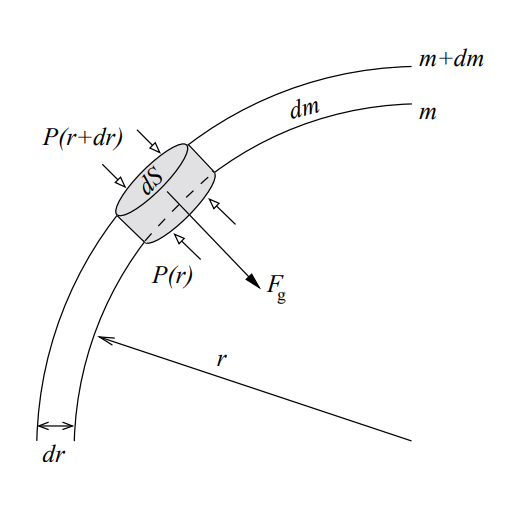
\includegraphics[scale=0.4]{Figures/spherical_shell_mechanical_equilibrium.png}
    \caption{Φλοιός σε ακτίνα $r$ και πάχος $dr$, μέσα σε σφαιρικά συμμετρικό αστέρι. Η μάζα του φλοιού είναι $dm = 4\pi r^2 \rho dr$. Στο σχήμα φαίνεται επίσης η πίεση και η βαρυτική δύναμη που ενεργούν σε ένα στοιχειώδες κυλινδρικό στοιχείο μάζας.}
    \label{fig:spherical_shell_hydrostatic_equilibrium}
\end{figure}

Η ολοκλήρωση της σχέσης \eqref{eq:mass_continuity_diff} μας δίνει την μάζα, $m(r)$, που περικλείει ένας σφαιρικός φλοιός ακτίνας $r$
\begin{equation}
        \label{eq:mass_coordinate}
    m(r) = \int_{0}^{R} 4\pi r^2 \rho(r) \,dr \hspace{0.5cm} (m \in 0,\dots,M)
\end{equation}

Επειδή η μάζα $m(r)$ αυξάνεται μονοτονικά προς την επιφάνεια του αστέρα, μπορούμε να χρησιμοποιήσουμε αυτή ως ακτινική συντεταγμένη αντί του $r$ (δηλαδή να χρησιμοποιήσουμε μια Λαγκραντζιανή περιγραφή αντί της μεθόδου του Euler). Έτσι η εξίσωση \eqref{eq:mass_coordinate} περιγράφει τη \textit{συντεταγμένη μάζας} (mass coordinate), η οποία είναι γενικευμένη συντεταγμένη (Lagrange coordinates) και κινείται μαζί με ένα στοιχειώδες κομμάτι του ρευστού. Αυτή η περιγραφή είναι προτιμότερη πολλές φορές καθώς η ακτίνα του αστέρα είναι συνάρτηση του χρόνου και μεταβάλλεται πολλές τάξεις μεγέθους κατά τη διάρκεια της εξέλιξής του.
Αντίθετα, η μάζα του μπορεί να θεωρηθεί σταθερή σε πρώτη φάση, γεγονός που απλοποιεί μερικές από τις χρονικές παραγώγους στις διαφορικές εξισώσεις που περιγράφουν την χημική σύσταση του αστέρα όπως θα δούμε. Έτσι, μπορούμε να γράψουμε όλες τις ποσότητες ως συνάρτηση της μάζας αντί του $r$ ως $r = r(m), \rho = \rho(m), P = P(m)$ κτλ. Κάνοντας τον μετασχηματισμό $r \rightarrow m$, η εξίσωση \eqref{eq:mass_continuity_diff} γράφεται ξανά:
\begin{equation}
    \label{eq:mass_continuity_diff_dm}
    \frac{d}{dm} = \frac{d}{dr} \cdot \frac{dr}{dm}  \longrightarrow \boxed{\frac{dr}{dm} = \frac{1}{4\pi r^2 \rho (r)}}
\end{equation}
%% ---------------------------------------------------------------------------------------------------- %%
%% ---------------------------------------------------------------------------------------------------- %%
%% ---------------------------------------------------------------------------------------------------- %%
\subsubsection{Το βαρυτικό πεδίο}
Τα αστέρια είναι αέρια σώματα που υποστηρίζονται από την ίδια τους την βαρύτητα (self-gravitating bodies), πράγμα που σημαίνει ότι η βαρύτητα παίζει καταλυτικό ρόλο στην εξέλιξή τους. Στη γενική, μη-σφαιρική περίπτωση, η βαρυτική επιτάχυνση είναι η κλίση (gradient) του βαρυτικού δυναμικού $\Phi$
$$\boldsymbol{g} = - \nabla \Phi$$
όπου το $\Phi$ είναι λύση της εξίσωσης Poisson 
\begin{equation}
    \label{eq:poisson_equation}
    \nabla^2 \Phi = 
    \begin{cases}
        0 & \text{για r > R}\\
        4\pi G \rho & \text{για r < R}
    \end{cases}
\end{equation}

Για μία σφαιρική κατανομή μάζας $M$, μπορούμε να θεωρήσουμε ότι όλη η μάζα είναι συγκεντρωμένη σε ένα σημείο στο κέντρο. Τότε, το βαρυτικό δυναμικό $\Phi$ σε απόσταση $r>R$ από το κέντρο, ισούται με το έργο ανά μονάδα μάζας που απαιτείται για να φέρουμε ένα σώμα μάζας $m$ από το άπειρο, σε αυτό το σημείο
\begin{equation}
    \Phi = \frac{1}{m}\int_{\infty}^{r} \boldsymbol{F_{\text{gr}}} \cdot d\boldsymbol{r} = \frac{1}{m} \int_{\infty}^{r} G\frac{M \,m }{r^2} \,dr \Rightarrow \Phi = - \frac{G \,M}{r}
\end{equation}
H βαρυτική επιτάχυνση γράφεται απλά $g = d\Phi / dr$ και σε ακτίνα $r$ (ή ισοδύναμα σε συντεταγμένη μάζας $m$) δίνεται από 
\begin{equation}
    \label{eq:gravitational_field}
    g = G \frac{m}{r^2}
\end{equation}
Σφαιρικοί φλοιοί που βρίσκονται σε ακτίνα μεγαλύτερη από $r$ δεν εφαρμόζουν κάποια δύναμη, άρα το $g$ εξαρτάται μόνο από την κατανομή της μάζας μέσα στον φλοιό ακτίνας $r$ (shell theorem). Το συμπέρασμα αυτό μπορεί να αποδειχθεί με τη βοήθεια του νόμου του Gauss από τον διανυσματικό λογισμό σύμφωνα με τον οποίο "το επιεπιφάνειο ολοκλήρωμα μια διανυσματικής συνάρτησης σε μια κλειστή επιφάνεια S ισούται με το τριπλό ολοκλήρωμα της απόκλισης (divergence) της διανυσματικής αυτής συνάρτησης στον όγκο V που περικλείεται από την κλειστή επιφάνεια"
\begin{equation}
    \label{eq:gauss_law_vector_calculus}
    \oiint_S \boldsymbol{f} \cdot d \boldsymbol{S} = \iiint_V (\nabla \cdot \boldsymbol{f}) \,dV 
\end{equation}
Θέτωντας $\boldsymbol{f} = \boldsymbol{g}$, προκύπτει ότι το αριστερό μέλος της σχέσης \eqref{eq:gauss_law_vector_calculus} γράφεται
\begin{equation}
    \label{eq:left_hand_side_gauss_law}
    \oiint_S \boldsymbol{g} \cdot d \boldsymbol{S} = \oiint_S (\boldsymbol{g} \cdot \hat{\eta}) \, dS = - 4\pi r^2 g
\end{equation}
Το παραπάνω αποτέλεσμα προκύπτει από τη σφαιρική συμμετρία του βαρυτικού πεδίου του αστέρα. Λόγω της συμμετρίας αυτής το πεδίο έχει μόνο ακτινική συνιστώσα, η οποία μάλιστα έχει σταθερή τιμή πάνω στη σφαιρική επιφάνεια S. Άρα, με την ένταση του βαρυτικού πεδίου να βγαίνει εκτός ολοκληρώματος, το κλειστό επικαμπύλιο ολοκλήρωμα ισούται με την επιφάνεια της σφαίρας με ακτίνα $r$. Το μείον προκύπτει επειδή το $\boldsymbol{g}$ με το διάνυσμα επιφάνειας $d\boldsymbol{S} = dS \cdot \hat{\eta}$ είναι συγγραμικά αλλά αντίρροπα.

Για το δεξιό μέλος της εξίσωσης \eqref{eq:gauss_law_vector_calculus}, πρέπει να βρούμε την απόκλιση της βαρυτικής επιτάχυνσης $(\nabla \boldsymbol{g})$. Από την εξίσωση Poisson (σχέση \eqref{eq:poisson_equation}), προκύπτει ότι
\begin{equation}
    \label{eq:right_hand_side_gauss_law}
    \nabla \boldsymbol{g} = \nabla (- \nabla \Phi) = - \nabla^2 \Phi = - 4\pi G \rho
\end{equation}
Συνδυάζοντας τις σχέσεις \eqref{eq:gauss_law_vector_calculus}, \eqref{eq:left_hand_side_gauss_law} και \eqref{eq:right_hand_side_gauss_law}, έχουμε ότι
\begin{equation}
    -4 \pi r^2 g = -4 \pi G \iiint_V \rho \,dV \Rightarrow g = G \frac{m(r)}{r^2}
\end{equation}
όπου το τριπλό ολοκλήρωμα μας δίνει απλά τη μάζα του αστέρα που περιέχεται μέσα σε μία σφαιρική επιφάνεια ακτίνας $r$ (σύμφωνα και με τη σχέση \eqref{eq:mass_coordinate}).
%% ---------------------------------------------------------------------------------------------------- %%
%% ---------------------------------------------------------------------------------------------------- %%
%% ---------------------------------------------------------------------------------------------------- %%
\subsubsection{Βαρυτική δυναμική ενέργεια}
Το να βρούμε τη συνολική βαρυτική δυναμική ενέργεια, $E_{\text{gr}}$, μιας μάζας όπως ο Ήλιος, φαίνεται εκ πρώτης όψεως μάταιο καθώς θα έπρεπε να αθροίσουμε τη δυναμική ενέργεια που προκαλεί κάθε ζεύγος σωματιδίων που αποτελούν τον Ήλιο. Το πρόβλημα απλουστεύται αν θεωρήσουμε ότι "κατασκευάζουμε" τον αστέρα με το να μεταφέρουμε στοιχειώδη σωματίδια από το άπειρο, ένα προς ένα (γι' αυτό και μερικές φορές αναφερόμαστε στην συνολική βαρυτική δυναμική ενέργεια ως ενέργεια σύνδεσης του αστέρα). Με αυτόν τον τρόπο, μεταφέρουμε ένα κομμάτι ύλης $dm$ στον μερικώς κατασκευασμένο αστέρα, που εκείνη τη στιγμή έχει μάζα $m$. Το κομμάτι αυτό της ύλης κατανείμεται συμμετρικά γύρω από τον αστέρα σχηματίζοντας έναν σφαιρικό φλοιό πάχους $dr$. Όπως είπαμε, η βαρυτική δύναμη που ασκείται σε ένα σωματίδιο έξω από μία σφαιρική κατανομή μάζας, όπως αυτή του Ήλιου, είναι ίδια σαν η μάζα να ήταν συγκεντρωμένη στο κέντρο του αστέρα. Γι' αυτό το λόγο, η δυναμική ενέργεια της μάζας $dm$ η οποία κατανέμεται συμμετρικά σε απόσταση $r$ από το κέντρο του αστέρα, είναι ίδια με τη δυναμική ενέργεια που θα είχαμε μεταξύ δύο σημειακών μαζών $dm$ και $m$ σε απόσταση $r$ μεταξύ τους. Έτσι, η διαφορά στη δυναμική βαρυτική ενέργεια του αστέρα θα ήταν
\begin{equation}
    dE_{\text{gr}} = E_{\text{gr}}^{dm}(r) - \cancelto{0}{E_{\text{gr}}^{dm}(\infty)} = - G \frac{m(r) \, dm}{r} 
\end{equation}
Ολοκληρώνοντας για όλες τις μάζες $dm$ μέσα στον φλοιό πάχους $dr$ σε απόσταση $r$ από το κέντρο έχουμε
\begin{equation}
    dE_{\text{gr}} = -G \int \frac{m(r) \,dm}{r} \xRightarrow{dm = \rho(r) \,dV} dE_{\text{gr}} = - G \frac{m(r) \,\rho(r) \, 4\pi r^2 \,dr}{r}
\end{equation}
όπου $dV = 4\pi r^2 \,dr$ ο όγκος του σφαιρικού φλοιού πάχους $dr$.

Ολοκληρώνοντας τώρα ως προς την ακτίνα του αστέρα, παίρνουμε την ολική βαρυτική δυναμική ενέργεια
\begin{equation}
    E_{\text{gr}} = -4\pi G \int_{0}^{R} m(r) \rho(r) \,r \,dr
\end{equation}
Γενικά, πρέπει να γνωρίζουμε το $\rho(r)$ για να βρούμε τη μάζα $m(r)$ η οποία είναι κι αυτή το ολοκλήρωμα
$$m(r) = \int_{0}^{m} dm = 4 \pi \int_{0}^{r} \rho(r) r^2 \,dr$$

Υποθέτωντας ότι 
\begin{equation}
    \rho(r) \approx \langle \rho \rangle = \frac{m}{\frac{4}{3} \pi R^3} \longrightarrow m(r) = \frac{4}{3} \pi r^3 \langle \rho \rangle
\end{equation}

Συνδυάζοντας όλα τα παραπάνω, προκύπτει τελικά ότι
\begin{align}
\label{eq:gravitational_potential_energy}
    \nonumber E_{\text{gr}} &= -4 \pi G \int_{0}^{R} \frac{4}{3} \pi r^3 \langle \rho \rangle^2 r \,dr \\\nonumber \\
    \nonumber &= -4\pi G \left( \frac{4\pi}{3} \right) \int_{0}^{R} r^4 \left( \frac{m}{\frac{4}{3} \pi R^3} \right)^2 \Rightarrow \\\nonumber \\
    &\Rightarrow \boxed{E_{\text{gr}} = - \frac{3Gm^2}{5R}}
\end{align}
%% ---------------------------------------------------------------------------------------------------- %%
%% ---------------------------------------------------------------------------------------------------- %%
%% ---------------------------------------------------------------------------------------------------- %%
\subsubsection{Υδροστατική ισορροπία}
Στη συνέχεια θα ασχοληθούμε με την αρχή διατήρησης της ορμής μέσα σε ένα αστέρι, δηλαδή με τον δεύτερο νόμο του Νεύτωνα. Η επιτάχυνση που δέχεται ένα στοιχειώδες κομμάτι αερίου καθορίζεται από το άθροισμα όλων των δυνάμεων που ενεργούν σε αυτό. Πέρα από την βαρυτική δύναμη, υπάρχουν και άλλες δυνάμεις που οφείλονται στην πίεση που ασκούν τα γειτονικά στρώματα αερίου πάνω στο υπο εξέταση στοιχειώδες κομμάτι. Λόγω της σφαιρικής συμμετρίας, οι δυνάμεις πίεσης που ασκούνται οριζόντια (κάθετα στην ακτινική διεύθυνση) εξισορροπούνται μεταξύ τους και άρα μόνο η δύναμη της πίεσης που ενεργεί κατά μήκος της ακτινικής διεύθυνσης πρέπει να ληφθεί υπόψιν. Άρα, η επιτάχυνση, $\boldsymbol{\ddot{r}}$, που δέχεται ένα στοιχειώδες κομμάτι αερίου μάζας
\begin{equation}
    \label{eq:dm}
    dm = \rho \,dr \,dS
\end{equation}
όπου $dr, dS$ είναι το στοιχειώδες πάχος και η στοιχειώδης οριζόντια επιφάνεια του κυλίνδρου (σχήμα \ref{fig:spherical_shell_hydrostatic_equilibrium}), θα είναι:
\begin{align}
    \label{eq:equation_of_motion_eulerian_coordinate}
    \nonumber dm \frac{\partial^2 \boldsymbol{r}}{\partial t^2} &\equiv \ddot{\boldsymbol{r}} \,dm = \boldsymbol{F}_{g} + \boldsymbol{F}_r + \boldsymbol{F}_{r+dr} = \\ \nonumber \\
    \nonumber & = -g \,dm + P(r) dS - P(r+dr) dS = \\ \nonumber \\
    \nonumber & = -g \,dm + dS \underbrace{\left[ P(r) - P(r+dr) \right]}_{-dP} = \\ \nonumber \\
    \nonumber & = -g \,dm - dP \,dS \Rightarrow \ddot{r} = -g - \frac{dP \,dS}{dm} \\ \nonumber \\
    &\xrightarrow[\text{\eqref{eq:gravitational_field}, \eqref{eq:dm}}]{\text{σχέσεις}} \ddot{r} = - G \frac{m}{r^2} - \frac{1}{\rho} \frac{dP}{dr}
\end{align}
Η σχέση \eqref{eq:equation_of_motion_eulerian_coordinate} είναι η \textit{εξίσωση κίνησης} για ένα στοιχειώδες κομμάτι αερίου μέσα στον αστέρα.

Xρησιμοποιώντας τη σχέση \eqref{eq:mass_continuity_diff_dm} στην βαθμίδα της πίεσης (pressure gradient), μπορούμε να γράψουμε ισοδύναμα την εξίσωση κίνησης εκφρασμένη σε συντεταγμένες μάζας ως
\begin{equation}
    \label{eq:equation_of_motion_lagrangian_coordinate}
    \ddot{r} = - G \frac{m}{r^2} - 4 \pi r^2 \frac{dP}{dm}
\end{equation}

Το γεγονός ότι η ακτίνα του Ήλιου παραμένει σταθερή εδώ και εκατομμύρια χρόνια, το γνωρίζουμε τόσο από ηλιακές όσο και γεωλογικές παρατηρήσεις. Εφόσον λοιπόν ο Ήλιος ούτε συστέλλεται ούτε διαστέλλεται, οι δυνάμεις που ασκούνται σε καθεμιά από τις δύο πλευρές κάθε επιφάνειας στο εσωτερικό του θα είναι ίσες και αντίθετες (σε αντίθετη περίπτωση η επιφάνεια αυτή δεν θα παρέμεινε ακίνητη). Με άλλα λόγια, η επιτάχυνση κατά την ακτινική διεύθυνση θα είναι μηδέν. Θέτωντας $\ddot{r} = 0$ στην εξίσωση κίνησης που δίνεται από τη σχέση \eqref{eq:equation_of_motion_eulerian_coordinate}, προκύπτει ότι
\begin{equation}
    \label{eq:hydrostatic_equilibrium_eulerian coordinates}
    \boxed{\frac{dP}{dr} = - G \frac{m(r) \rho(r)}{r^2}}
\end{equation}
ή, ισοδύναμα, σε συντεταγμένες μάζας
\begin{equation}
    \label{eq:hydrostatic_equilibrium_lagrangian_coordinate}
    \boxed{\frac{dP}{dm} = - G \frac{m(r)}{4\pi r^4}}
\end{equation}

Η εξίσωση \eqref{eq:hydrostatic_equilibrium_eulerian coordinates} αποτελεί τη δεύτερη διαφορική εξίσωση της αστρικής δομής, ονομάζεται εξίσωση \textit{υδροστατικής ισορροπίας}, και ισχύει όταν ο αστέρας βρίσκεται σε μηχανική ισορροπία (όταν δηλαδή οι δυνάμεις που ασκούνται σε ένα στοιχειώδες κομμάτι αερίου, εξισορροπούνται μεταξύ τους). Μαζί με την εξίσωση συνέχειας της μάζας (σχέση \eqref{eq:mass_continuity_diff}), προσδιορίζουν την \textit{μηχανική δομή} (mechanical structure) ενός αστέρα.

Άμεση συνέπεια της εξίσωσης \eqref{eq:hydrostatic_equilibrium_eulerian coordinates}, είναι ότι η πίεση σε έναν αστέρα που βρίσκεται σε υδροστατική ισορροπία \textit{πρέπει} να αυξάνεται όσο πλησιάζουμε το κέντρο του, ώστε να μπορεί να υποστηρίξει το βάρος των υπερκείμενων στρωμάτων.\\

{\color{red} \hrule}
\underline{Παρατήρηση}: Ένα αντικείμενο για να βρίσκεται σε κατάσταση υδροστατικής ισορροπίας, πρέπει να έχει αρκετή μάζα ώστε η βαρυτική δύναμη να είναι υπολογίσιμη. Έτσι, σώματα όπως η Σελήνη ή η Γη βρίσκονται σε κατάσταση υδροστατικής ισορροπίας, αλλά αντικείμενα όπως οι αστερεοιδείς όχι. Τα αντικείμενα αυτά υποστηρίζονται από τη φυσική ακαμψία τους (rigidity) η οποία οφείλεται στις ηλεκτρομαγνητικές αλληλεπιδράσεις των μορίων που τα αποτελούν.\\
{\color{red} \hrule}

Αξίζει να σημειωθεί ότι για να καταλήξουμε στην εξίσωση \eqref{eq:hydrostatic_equilibrium_eulerian coordinates} δεν κάναμε καμία υπόθεση για τη φύση της πίεσης που υπεισέρχεται στην εξίσωση αυτή, δηλαδή για τους μικροφυσικούς μηχαισμούς που παρουσιάζονται μακροσκοπικά ως πίεση. Από τη βασική Φυσική είναι γνωστοί ήδη δύο τέτοιοι μηχανισμοί, που μακροσκοπικά χαρακτηρίζονται ως \textit{πίεση αερίου}, $P_{\text{gas}}$, και \textit{πίεση ακτινοβολίας}, $P_{\text{rad}}$. Στη συνέχεια θα συναντήσουμε και έναν τρίτο μηχανισμό, που χαρακτηρίζεται μακροσκοπικά ως \textit{πίεση εκφυλισμένης ύλης}, $P_{\text{deg}}$. Στη γενικότερη περίπτωση λοιπόν θα πρέπει να χρησιμοποιούμε την ολική πίεση
$$ P = P_{\text{gas}} + P_{\text{rad}} + P_{\text{deg}}$$
όπου η πίεση του αερίου δίνεται από τον νόμο των τέλειων αερίων (σχέση \eqref{eq:ideal_gas_eos}), και η πίεση της ακτινοβολίας, $P_{\text{rad}}$, από τη σχέση \eqref{eq:radiation_pressure_black_body}. Ευτυχώς στο μεγαλύτερο ποσοστό των αστέρων, μεταξύ των οποίων συμπεριλαμβάνεται και ο Ήλιος, η πίεση της ακτινοβολίας και η πίεση της εκφυλισμένης ύλης είναι αμελητέες συγκρινόμενες με την πίεση του αερίου, και μπορούμε άνετα να τις παραλέιψουμε. Οι πιέσεις $P_{\text{rad}}$ και $P_{\text{deg}}$ γίνονται σημαντικές στις περιπτώσεις των πολύ μεγάλων, σε μάζα, αστέρων (η πρώτη) και των πολύ μικρών, σε διαστάσεις, αστέρων (η δεύτερη). Η ολοένα και αυξανόμενη πίεση της ακτινοβολίας όσο αυξανεται η μάζα των αστέρων είναι αυτή που θέτει και ένα ανώτερο όριο στη μάζα που μπορεί να έχει ένας αστέρας. Από κάποια οριακή τιμής της μάζας και πάνω, η πίεση της ακτινοβολίας είναι τόσο μεγάλη που καταστρέφει το αστέρι.
%% ---------------------------------------------------------------------------------------------------- %%
%% ---------------------------------------------------------------------------------------------------- %%
%% ---------------------------------------------------------------------------------------------------- %%
\subsubsection{Καταστατικές εξισώσεις}
Οι εξισώσεις \eqref{eq:mass_continuity_diff_dm} και \eqref{eq:hydrostatic_equilibrium_lagrangian_coordinate}
αποτελούν ένα σύστημα δύο εξισώσεων με τρεις αγνώστες συναρτήσεις του $m$ ($r$, $P$ και $\rho$), οπότε δεν μπορούν να λυθούν χωρίς μία τρίτη συνθήκη. Αυτή η συνθήκη είναι συνήθως μία σχέση μεταξύ της πίεσης, $P$, και της πυκνότητας μάζας, $\rho$, την οποία ονομάζουμε \textit{καταστατική εξίσωση} (equation of state). Γενικά, η καταστατική εξίσωση εξαρτάται και από τη θερμοκρασία, $T$, οπότε η μηχανική δομή ενός αστέρα εξαρτάται επίσης και από την κατανομή της θερμοκρασίας στο εσωτερικό του, δηλαδή από τη θερμική δομή του. Σε κάποιες ειδικές περιπτώσεις, η καταστατική εξίσωση είναι ανεξάρτητη της $T$, και μπορεί να γραφτεί ως $P = P(\rho)$. Σε αυτές τις περιπτώσεις (γνωστές ως βαρυτροπικές ή πολυτροπικές), η μηχανική δομή ενός αστέρα γίνεται ανεξάρτητη από τη θερμική δομή του. Μία τέτοια περίπτωση είναι αυτή των λευκών νάνων όπως θα δούμε στη συνέχεια.

Γίνεται αντιληπτό πως η καταστατική εξίσωση περιγράφει τις μικροσκοπικές ιδιότητες της αστρικής ύλης, για μία δεδομένη πυκνότητα μάζας $\rho$, θερμοκρασία $T$, και χημικής σύστασης $X_i$. Συνήθως εκφράζεται ως σχέση μεταξύ της πίεσης και αυτών των ποσοτήτων:
\begin{equation}
    P = P(\rho, T, X_i)
\end{equation}

Αν θεωρήσουμε αρχικά για λόγους απλότητας πως ένας αστέρας αποτελείται εξ' ολοκλήρου από Υδρογόνο και συμπεριφέρεται ως ιδανικό αέριο, τότε η καταστατική εξίσωση θα δίνεται από την γνωστή καταστατική εξίσωση των τέλειων αερίων 
\begin{equation}
    P(r) = n(r) kT = \frac{\rho}{m_\text{H}} kT
\end{equation}
Θεωρώντας τώρα ότι ένας αστέρας αποτελείται από διάφορα χημικά στοιχεία, η μάζα μπορεί να αντικατασταθεί από τη μέση μάζα του αέριου μείγματος, $\overline{m}$, ώστε
\begin{equation}
    P = \frac{\rho}{\overline{m}} kT
\end{equation}

Ορίζοντας την ποσότητα του \textit{μέσου μοριακού βάρους}
\begin{equation}
    \mu \equiv \frac{\overline{m}}{m_{\text{H}}}
\end{equation}
η καταστατική εξίσωση για ένα μείγμα ιδανικού αερίου θα είναι
\begin{equation}
    \label{eq:ideal_gas_eos}
    \boxed{P = \frac{\rho}{\mu m_{\text{H}}} k T }
\end{equation}
Προφανώς ο βαθμός ιονισμού του αερίου, κβαντομηχανικά (εκφυλισμός) και σχετικιστικά φαινόμενα επηρεάζουν την μορφή της καταστατικής εξίσωσης που πρέπει να λάβουμε υπόψιν κάθε φορά που θέλουμε να μελετήσουμε τη δομή ενός αστέρα. 

Η πίεση σχετίζεται και με την εσωτερική ενέργεια ενός αερίου. Για καταστατικές εξισώσεις αερίων που δεν είναι ιδανικά, υπάρχει μία σχέση μεταξύ της πίεσης και της εσωτερικής ενέργειας, την οποία μπορούμε να γράψουμε γενικά
\begin{equation}
    \label{eq:generic_eos}
    E_{\text{int}} = \phi \frac{P}{\rho} 
\end{equation}
Για το ιδανικό αέριο, η μέση εσωτερική ενέργεια ισούται με τη μέση κινητική ενέργεια (λόγω της θερμικής κίνησης των σωματιδίων) καθώς σε ένα μονοατομικό ιδανικό αέριο, τα σωματίδια δεν δονούνται και δεν περιστέφονται. Έτσι, μόνο η συνεισφορά της θερμικής (κινητικής) ενέργειας λαμβάνεται υπόψιν ώστε
\begin{equation}
    \label{eq:internal_energy_ideal_gas}
    \frac{\langle  E_{\text{int}} \rangle}{N} = \frac{\langle  E_{\text{kin}} \rangle}{N} = \frac{3}{2}kT
\end{equation}
όπου $N=\overline{m}/(\mu m_{\text{H}})$ είναι ο αριθμός των σωματιδίων. Oπότε για την περίπτωση του ιδανικού αερίου, $\phi = 3/2$. Αποδεικνύεται ότι αυτό ισχύει όχι μόνο στην περίπτωση του ιδανικού αερίου, αλλά για όλα τα μη-σχετικιστικά σωματίδια. Αντίθετα, αν θεωρήσουμε ένα αέριο που αποτελείται από σχετικιστικά σωματίδια, κυρίως φωτόνια (πίεση ακτινοβολίας), τότε προκύπτει ότι $\phi = 3$.

Με την καταστατική εξίσωση βρήκαμε μία σχέση μεταξύ της πίεσης και της πυκνότητας μάζας, αλλά εμφανίστηκε η άγνωστη παράμετρος της θερμοκρασίας. Το ότι η θερμοκρασία δεν είναι σταθερή σε όλη τη μάζα του αστέρα το γνωρίζουμε από διάφορα παρατηρησιακά δεδομένα όπως έχουμε πει, π.χ. αμαύρωση του χείλους, γραμμές απορρόφησης, και ότι το συνεχές φάσμα δεν ταυτίζεται με αυτό του μέλανος σώματος. Χρειαζόμαστε άρα και μία εξίσωση για το πως αλλάζει η θερμοκρασία προκειμένου να κλείσει το σύστημα των εξισώσεων.
%% ---------------------------------------------------------------------------------------------------- %%
%% ---------------------------------------------------------------------------------------------------- %%
%% ---------------------------------------------------------------------------------------------------- %%
\subsubsection{Θεώρημα virial}
Μία από τις συνέπεις της υδροστατικής ισορροπίας, είναι το θεώρημα virial. Το θεώρημα αυτό είναι παίζει καθοριστικό ρόλο σε διάφορα πεδία της Αστροφυσικής καθώς συνδέει δύο διαθέσιμες "δεξαμενές" ενέργειας επιτρέποντάς μας να ερμηνεύσουμε και να κάνουμε προβλέψεις για διάφορες φάσεις της αστρικής εξέλιξης.

Για να καταλήξουμε στο θεώρημα virial ξεκινάμε από την εξίσωση υδροστατικής ισορροπίας, \eqref{eq:hydrostatic_equilibrium_lagrangian_coordinate}. Πολλαπλασιάζοντας τα δύο μέλη με τον εσώκλειστο όγκο $V = \frac{4}{3}\pi r^3$ και ολοκληρώνοντας ως προς τη μάζα έχουμε
\begin{align*}
    \int_{0}^{M} \frac{4}{3} \pi r^3 \frac{dP}{dm} \,dm  = - \frac{1}{3} \underbrace{\int_{0}^{M} \frac{G \,m}{r} \,dm}_{= - E_{\text{gr}}} \Rightarrow \int_{\text{C}}^{\text{S}} V \,dP = \frac{1}{3} E_{\text{gr}}
\end{align*}
όπου οι τιμές S, C δηλώνουν επιφανειακές και κεντρικές τιμές αντίστοιχα. Το ολοκλήρωμα στο αριστερό μέλος μπορεί να λυθεί κατά παράγοντες ώστε
\begin{align}
    \label{eq:generic_form_virial}
    \nonumber &\left. V \,P \right|_{\text{C}}^{\text{S}} - \int_{\text{C}}^{\text{S}} P \,dV = \frac{1}{3} E_{\text{gr}} \Rightarrow V_{\text{S}}  \,\cancelto{0}{P_{\text{S}}} - \cancelto{0}{V_{\text{C}}} \,P_{\text{C}} - \\ \nonumber \\
    &- \int_{\text{C}}^{\text{S}} P \,dV = \frac{1}{3} E_{\text{gr}} \xRightarrow{dV = \rho \,dm} \boxed{E_{\text{gr}} = -3 \int_{0}^{M} \frac{P}{\rho} \,dm}
\end{align}

Η σχέση \eqref{eq:generic_form_virial} αποτελεί τη γενική μορφή του θεωρήματος virial και μας δείχνει ότι η μέση πίεση που χρειάζεται για να υποστηριχτεί ένας αστέρας σε υδροστατική ισορροπία είναι ίση με το $- \frac{1}{3} \frac{E_{\text{gr}}}{V}$. Συγκεκριμένα, μας δείχνει ότι ένας αστέρας ο οποίος συστέλλεται σχεδόν στατικά (δηλαδή αρκετά αργά ώστε να παραμένει σε υδροστατική ισορροπία) πρέπει να αυξάνει την εσωτερική του πίεση, αφού η βαρυτική δυναμική ενέργεια, $E_{\text{gr}}$, μειώνεται όσο μικραίνει η ακτίνα του αστέρα και γίνεται πιο συμπαγές (more tightly bound).


Όπως έχουμε πει, η πίεση σχετίζεται με την εσωτερική ενέργεια ενός αερίου. Στην περίπτωση που το αέριο αυτό είναι ιδανικό, τότε από τις σχέσεις \eqref{eq:ideal_gas_eos}, \eqref{eq:internal_energy_ideal_gas} και \eqref{eq:generic_form_virial}, προκύπτει ότι 
\begin{align*}
    \langle E_{\text{int}} \rangle = \langle E_{\text{kin}} \rangle = \frac{3}{2} \frac{P}{\rho} \mu m_{\text{H}} \longrightarrow u = \frac{\langle E_{\text{int}} \rangle}{\mu m_{\text{H}}}
\end{align*}
όπου με $u$ συμβολίζουμε την εσωτερική ενέργεια ανά μονάδα μάζας, και άρα η μορφή του θεωρήματος virial είναι
\begin{equation}
    \label{eq:ideal_gas_virial}
    E_{\text{gr}} = -3 \int_{0}^{M} \frac{P}{\rho} \,dm = - 2 \underbrace{\int_{0}^{M} u \,dm}_{E_{\text{int}}} \rightarrow \boxed{E_{\text{int}} = - \frac{1}{2} E_{\text{gr}}}
\end{equation}
 
Η σχέση \eqref{eq:ideal_gas_virial} θεμελιώνει ένα σύνδεσμο μεταξύ της βαρυτικής δυναμικής ενέργειας και της εσωτερικής (θερμικής) ενέργειας ενός αστέρα σε υδροστατική ισορροπία, ο οποίος αποτελείται από ιδανικό αέριο. Το θεώρημα virial μας λέει ότι όσο πιο συμπαγής γίνεται ένας αστέρας θα πρέπει να έχει και μεγαλύτερη εσωτερική ενέργεια, δηλαδή να είναι πιο θερμός. Με άλλα λόγια, ένας αστέρας που συστέλλεται σχεδόν στατικά πρέπει να γίνεται ολοένα και θερμότερος κατά τη διάρκεια της διαδικασίας. Το τι συνεπάγεται αυτό θα φανεί σε λίγο όταν αναλογιστούμε την ολική ενέργεια του αστέρα.

Στην περίπτωση που το αέριο δεν μπορεί να θεωρηθεί ιδανικό, δείξαμε ότι η σχέση μεταξύ της πίεσης και της εσωτερικής ενέργειας θα δίνεται από μία σχέση της μορφής της \eqref{eq:generic_eos}. Για $\phi = 3/2$ το αέριο είναι ιδανικό, ενώ για $\phi = 3$ το αέριο αποτελείται από σχετικιστικά σωματίδια. Αν το $\phi$ είναι σταθερό, τότε ολοκληρώνοντας τη σχέση \eqref{eq:generic_form_virial}, καταλήγουμε σε μια ακόμα πιο γενική μορφή του θεωρήματος virial
\begin{equation}
    \label{eq:generic_eos_virial}
    E_{\text{gr}} = - \frac{3}{\phi} \int_{0}^{M} \langle E_{\text{int}} \rangle \,dm \Rightarrow \boxed{ E_{\text{int}} = - \frac{1}{3} \phi  E_{\text{gr}}}
\end{equation}
%% ---------------------------------------------------------------------------------------------------- %%
%% ---------------------------------------------------------------------------------------------------- %%
%% ---------------------------------------------------------------------------------------------------- %%
\subsubsection{Ολική ενέργεια αστέρων}
Η ολική ενέργεια ενός αστέρα είναι το άθροισμα της βαρυτικής δυναμικής ενέργειας, της εσωτερικής του ενέργειας, και της κινητικής ενέργειας (λόγω της μαζικής κίνησης --bulk motion-- του αερίου μέσα στον αστέρα και όχι λόγω της θερμικής κίνησης των σωματιδίων του αερίου).
\begin{equation}
    \label{eq:total_energy_of_star_generic}
    E_{\text{tot}} =  E_{\text{gr}} +  E_{\text{int}} +  E_{\text{kin}}
\end{equation}
Ένας αστέρας εξακολουθεί να είναι δέσμιος (bound) όσο η ολική του ενέργεια είναι \textbf{αρνητική}.

Για έναν αστέρα σε υδροστατική ισορροπία μπορούμε να θέσουμε $ E_{\text{kin}} = 0$. Επίσης, για τον αστέρα που βρίσκεται σε υδροστατική ισορροπία ισχύει το θεώρημα virial, οπότε η $E_{\text{gr}}$ και η $E_{\text{int}}$ είναι στενά συνδεδμένες μέσω της σχέσης \eqref{eq:generic_eos_virial}. Συνδυάζοντας τις σχέσεις \eqref{eq:generic_eos_virial} και \eqref{eq:total_energy_of_star_generic} προκύπτουν οι ακόλουθες σχέσεις
\begin{equation}
    \label{eq:total_energy_of_star_with_generic_eos}
    E_{\text{tot}} = E_{\text{gr}} + E_{\text{int}} = \left( \frac{\phi - 3}{\phi} \right) E_{\text{int}} = \left( 1 - \frac{\phi}{3} \right) E_{\text{gr}}
\end{equation}
Παρατηρούμε ότι όσο το $\phi < 3$, ο αστέρας είναι δέσμιος. Αν θέσουμε $\phi = 3/2$, παίρνουμε την περίπτωση του ιδανικού αερίου οπότε η σχέση \eqref{eq:total_energy_of_star_with_generic_eos} γράφεται
\begin{equation}
    \label{eq:total_energy_of_star_ideal_gas}
     \boxed{E_{\text{tot}} = -  E_{\text{int}} = \frac{1}{2}  E_{\text{gr}} < 0}
\end{equation}
δηλαδή βλέπουμε πως για έναν τέτοιον αστέρα, η ολική του ενέργεια ισούται με το μισό της βαρυτικής δυναμικής του ενέργειας. 

Αν η κυρίαρχη πίεση στο εσωτερικό ενός αστέρα είναι η πίεση της ακτινοβολίας ($\phi = 3$), τότε βλέπουμε ότι η ολική του ενέργεια ισούται με μηδέν, καθώς $ E_{\text{int}} = -  E_{\text{gr}}$. Για αυτό το λόγο, αστέρες που υποστηριζόνται από την πίεση σχετικιστικών σωματιδίων είναι οριακά δέσμιοι, και συνεπώς εξαιρετικά ευαίσθητοι σε διαταραχές που μπορούν να οδηγήσουν στην κατάρρευση ή την έκρηξη του αστέρα. 


Από την σχέση \eqref{eq:total_energy_of_star_ideal_gas} προκύπτει ότι το θεώρημα virial έχει τις εξής συνέπειες:

\begin{itemize}
    \item Βαρυτικά δέσμιες σφαίρες αερίων πρέπει να είναι θερμές για να διατηρήσουν υδροστατική ισορροπία: η θερμότητα παρέχει την πίεση που απαιτείται για να εξισορροπιστεί η βαρύτητα. Όσο πιο συμπαγές είναι μία τέτοια σφαίρα, τόσο πιο δέσμια θεωρείται, και άρα περισσότερο θερμή.
    
    \item Μία θερμή σφαίρα αερίων ακτινοβολεί ενέργεια στον τριγύρω χώρο σύμφωνα με τον νόμο των Stefan-Boltzmann. Άρα, ο αστέρας πρέπει να χάνει ενέργεια από την επιφάνειά του. Ο ρυθμός με τον οποίο ακτινοβολείται αυτή η ενέργεια από την επιφάνεια είναι η λαμπρότητα του αστέρα. Αν δεν υπάρχει κάποια εσωτερική πηγή ενέργειας, τότε αυτή η απώλεια ενέργειας πρέπει να είναι ίση με την μείωση της ολικής ενέργειας του αστέρα
    \begin{equation}
        L = - \frac{dE_{\text{tot}}}{dt} > 0
    \end{equation}
    εφόσον θεωρούμε ότι το $L$ είναι θετικό.
    
    \item Παίρνοντας την χρονική παράγωγο της σχέσης \eqref{eq:total_energy_of_star_ideal_gas}, βρίσκουμε ότι ως συνέπεια του ότι ο αστέρας χάνει ενέργεια:
    \begin{equation}
        \Dot{E}_{\text{gr}} = - 2L < 0    
    \end{equation}
    δηλαδή ο αστέρας συστέλλεται (γίνεται πιο δέσμιος), καθώς επίσης
    \begin{equation}
        \Dot{E}_{\text{int}} = L > 0
    \end{equation}
    που σημαίνει ότι ο αστέρας γίνεται πιο θερμός --- σε αντίθεση με τα καθημερινά αντικείμενα όπου γίνονται πιο ψυχρά καθώς χάνουν ενέργεια. Γι' αυτό το λόγο, ένας αστέρες λέγεται ότι έχει \textit{αρνητική θερμοχωρητικότητα}. Η μισή ενέργεια που απελευθερώνεται από τη συστολή του αστέρα χρησιμοποιείται για τη θέρμανση του αστέρα, ενώ η άλλη μισή ακτινοβολείται από την επιφάνεια.
    
    \item Όσο ο αστέρας είναι στην κύρια ακολουθία μετατρέποντας Υδρογόνο σε Ήλιο (όπως θα δούμε αργότερα μέσω θερμοπυρηνικής σύντηξης), το μέσο μοριακό βάρος του αυξάνεται. Αυτό οδηγεί σε μεγαλύτερη εσωτερική ενέργεια, και σύμφωνα με το θεώρημα virial ο αστέρας πρέπει να συσταλλέι προκειμένου να διατηρήσει την πίεση που χρειάζεται ώστε να αντισταθμιστεί η βαρύτητα.
\end{itemize}
%% ---------------------------------------------------------------------------------------------------- %%
%% ---------------------------------------------------------------------------------------------------- %%
%% ---------------------------------------------------------------------------------------------------- %%
\subsubsection{Κεντρική πίεση και θερμοκρασία αστέρων}
Μπορούμε να έχουμε μία εκτίμηση για την τάξη μεγέθους της πίεσης που επικρατεί στο κέντρο των αστέρων αν θέσουμε στην εξίσωση \eqref{eq:hydrostatic_equilibrium_lagrangian_coordinate},
        \begin{equation}
            \frac{dP}{dm} \sim \frac{\cancelto{0}{P_{\text{S}}} - P_{\text{C}}}{M_{\text{S}} - \cancelto{0}{M_{\text{C}}}} \,\approx - \frac{P_{\text{C}}}{M}
        \end{equation}
        όπου υποθέσαμε ότι η πίεση στην επιφάνεια και η μάζα στο κέντρο του αστέρα είναι πρακτικά μηδέν. Θέτωντας $m \sim \frac{1}{2} M $ και $r \sim \frac{1}{2} R$ στο δεύτερο μέλος της σχέσης \eqref{eq:hydrostatic_equilibrium_lagrangian_coordinate}, προκύπτει ότι 
        \begin{equation}
            \label{eq:estimation_of_central_pressure}
            \boxed{P_{\text{C}} \sim \frac{2}{\pi} \frac{G M^2}{R^4}}
        \end{equation}
        Στο ίδιο αποτέλεσμα καταλήγουμε και αν ολοκληρώσουμε την εξίσωση της υδροστατικής ισορροπίας, θεωρώντας την πυκνότητα σταθερή $\langle \rho \rangle \approx 3M/(4\pi R^3)$.
        
        Για τον Ήλιο, η σχέση \eqref{eq:estimation_of_central_pressure} μας δίνει $$P_{\text{C}} \sim 7 \times 10^9 \,\text{atm} \,= 7 \times 10^{15} \,\text{dyn/cm$^2$}$$
        
        Μπορούμε να βρούμε ένα κατώτερο όριο για την κεντρική πίεση αν γράψουμε τη σχέση \eqref{eq:hydrostatic_equilibrium_lagrangian_coordinate} ως
        \begin{align*}
            \frac{dP}{dr} &= - \frac{Gm}{4\pi r^4} \frac{dm}{dr} = - \frac{d}{dr} \left( \frac{Gm^2}{8\pi r^4} \right) - \frac{Gm^2}{2\pi r^5} \Rightarrow \\\\
            &\Rightarrow \frac{d}{dr} \underbrace{\left( P + \frac{G m^2}{8 \pi r^4} \right)}_{\Psi(r)} = - \frac{G m^2}{2\pi r^5} < 0
        \end{align*}
        Η ποσότητα $\displaystyle \Psi(r) = P + \frac{G m^2}{8 \pi r^4}$, είναι λοιπόν μία συνάρτηση που μειώνεται με το $r$. Στο κέντρο του αστέρα, ο δεύτερος όρος μηδενίζεται επειδή $m \propto r^3$ για μικρά $r$, οπότε $\Psi(0) = P_{\text{C}}$. Στην επιφάνεια του αστέρα, η πίεση είναι πρακτικά μηδέν και άρα $\displaystyle \Psi(R) = \frac{GM^2}{8\pi R^4}$. Αφού η ποσότητα $\Psi$ πρέπει να μειώνεται με την απόσταση $r$, συνεπάγεται πως $\Psi(0) > \Psi(R)$ και άρα
        \begin{equation}
            \label{eq:lower_limit_of_central_pressure_for_stars_in_HE}
            P_{\text{C}} > \frac{1}{8\pi} \frac{GM^2}{R^4}
        \end{equation}
        
        Σε αντίθεση με την σχέση \eqref{eq:estimation_of_central_pressure}, αυτό είναι ένα αυστηρό μαθηματικό αποτέλεσμα που ισχύει για κάθε αστέρα σε υδροστατική ισορροπία, ανεξάρτητα από τις άλλες ιδιότητές του (συγκεκριμένα, ανεξάρτητα από την κατανομή της πυκνότητάς του). Για τον Ήλιο προκύπτει ότι $P_{\text{C}} > 4.4 \times 10^{14} \,\text{dyn/cm$^2$}$. Και οι δύο εκτιμήσεις δείχνουν ότι χρειάζονται πολύ υψηλές τιμές της κεντρικής πίεσης για να κρατήσουν τον Ήλιο σε υδροστατική ισορροπία.
        
        
        Χρησιμοποποιώντας το θεώρημα virial μπορούμε να κάνουμε μία εκτίμηση για την μέση θερμοκρασία που επικρατεί σε έναν αστέρα που αποτελείται από ιδανικό αέριο. Η βαρυτική ενέργεια βρήκαμε από τη σχέση \eqref{eq:gravitational_potential_energy} ότι είναι
        \begin{equation*}
            E_{\text{gr}} = - \alpha \frac{GM^2}{R}
        \end{equation*}
        όπου η σταθερά $\alpha$ είναι της τάξης της μονάδας και καθορίζεται από την κατανομή της μάζας στον αστέρα, δηλαδή το προφίλ της πυκνότητάς του. Η εσωτερική ενέργεια θα είναι
        \begin{align*}
            u &= \frac{3}{2} \frac{kT}{\mu m_{\text{H}}} = \frac{E_{\text{int}}}{\mu m_{\text{H}}} = \frac{3}{2} \frac{P}{\rho}  \longrightarrow \\\\
            E_{\text{int}} &= \frac{3}{2} \frac{k}{\mu m_{\text{H}}} \int T \,dm = \frac{3}{2} \frac{k}{\mu m_{\text{H}}} \langle T \rangle M
        \end{align*}
        όπου $\langle T \rangle$ είναι η μέση θερμοκρασία υπολογισμένη σε όλους τους φλοιούς. Έτσι, από το θεώρημα virial έχουμε
        \begin{equation}
            2 E_{\text{int}} = - E_{\text{gr}} \longrightarrow \langle T \rangle = \frac{\alpha}{3} \frac{\mu m_{\text{H}}}{k} \frac{GM}{R}
        \end{equation}
        Θέτωνας $\alpha \approx 1$ και $\mu = 0.5$ για ιονισμένο Υδρογόνο, προκύπτει ότι για τον Ήλιο
        $\langle T \rangle \sim 4 \times 10^6 \,\text{K}$. Αυτή είναι η μέση θερμοκρασία που απαιτείται για να παρέχει την κατάλληλη πίεση ώστε να κρατάει τον Ήλιο σε υδροστατική ισορροπία. Επειδή η θερμοκρασία σε έναν αστέρα συνήθως μειώνεται όσο πλησιάζουμε την επιφάνεια, αυτή η εκτίμηση είναι επίσης και ένα κατώτερο όριο για την κεντρική θερμοκρασία του Ήλιου. Σε αυτές τις θερμοκρασίες, το Υδρογόνο και το Ήλιο είναι όντως τελείως ιονισμένα.
%% ---------------------------------------------------------------------------------------------------- %%
%% ---------------------------------------------------------------------------------------------------- %%
%% ---------------------------------------------------------------------------------------------------- %%
\subsection{Θερμική ισορροπία}
Από παρατηρήσεις γνωρίζουμε πως ο Ήλιος συνεχώς εκπέμπει ενέργεια από την επιφάνειά του αλλά η $T_{\text{eff}}$ παραμένει περίπου σταθερή. Αυτό σημαίνει πως ο Ήλιος βρίσκεται σε μία στατική κατάσταση.
Εαν υπάρχουν εσωτερικές πηγές ενέργειας στους αστέρες, τότε η ενέργεια που χάνεται από την επιφάνεια μπορεί να αναπληρωθεί:
$$L = L_{\text{source}} = - \frac{dE_{\text{source}}}{dt}$$
Σε αυτή την περίπτωση, η ολική ενέργεια του αστέρα διατηρείται και η εξίσωση \eqref{eq:total_energy_of_star_ideal_gas} μας λέει ότι
$$\Dot{E}_{\text{tot}} = \Dot{E}_{\text{int}} = \Dot{E}_{\text{gr}} = 0$$
Το θεώρημα virial μας υποδεικνύει τότε πως οι $E_{\text{int}}, E_{\text{gr}}$ διατηρούνται επίσης: ο αστέρας δεν μπορεί για παράδειγμα να συσταλλεί και να ψυχθεί ενώ διατηρεί την ολική του ενέργεια σταθερή.

Σε αυτή την στατική κατάσταση, την οποία θα ονομάζουμε \textbf{θερμική ισορροπία}, η ενέργεια ακτινοβολείται από την επιφάνεια του αστέρα με τον ίδιο ρυθμό που παράγεται στο εσωτερικό του. Ο αστέρας δεν συστέλλεται ούτε διαστάλλεται, διατηρώντας μία σταθερή εσωτερική θερμοκρασία. Όπως θα δούμε, αυτή η θερμοκρασία ρυθμίζεται από τις πυρηνικές αντιδράσεις που συμβαίνουν στον πυρήνα του, που σε συνδυασμό με το θεώρημα virial λειτουργούν ως αστρικός θερμοστάτης. Αυτό συμβαίνει γιατί αν η ενέργεια διαφεύγει με ταχύτερο ρυθμό απ' ότι παράγεται, τότε το εσωτερικό ψύχεται. Αυτό σημαίνει ότι ελλατώνεται η πίεση του αερίου, και ο αστέρας συστέλλεται. Αλλά όσο ο αστέρας συστέλλεται, η πυκνότητα αυξάνει και η απελευθέρωση της βαρυτικής δυναμικής ενέργειας πηγαίνει στη θέρμανση του υλικού. Αυτή η διαδικασία αυξάνει τον ρυθμό των πυρηνικών αντιδράσεων, παράγωντας περισσότερη ενέργεια. Όταν επέλθει μία ισορροπία μεταξύ του ρυθμού παραγωγής ενέργειας και την ροή της διαφεύγουσας ενέργειας, ο αστέρας έχει φτάσει σε μία σταθερή θερμική δομή, και δεν χρειάζονται περισσότερες προσαρμογές στην δομή.
Αστέρες της κύριας ακολουθίας, όπως ο Ήλιος, είναι σε θερμική ισορροπία και παραμένουν σε αυτή την κατάσταση για όσο διάστημα οι πυρηνικές αντιδράσεις μπορούν να παρέχουν την κατάλληλη ενέργεια.

\begin{figure}[h]
    \centering
    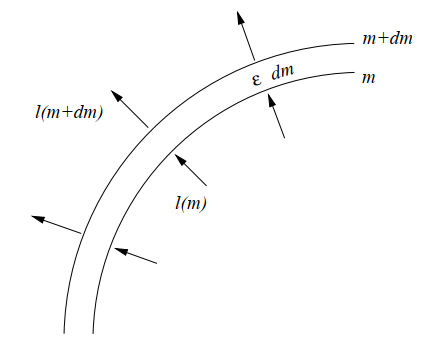
\includegraphics[scale=0.5]{Figures/thermal_equilibrium_scheme.png}
    \caption{Παραγωγή ενέργειας και ροή θερμότητας προς και από σφαιρικό φλοιό μάζας $dm$.}
    \label{fig:thermal_equilibrium_scheme}
\end{figure}

Έστω ότι θεωρούμε έναν σφαιρικό, Λαγκραντζιανό φλοιό σταθερής μάζας $dm$ μέσα σε έναν αστέρα (σχήμα \ref{fig:thermal_equilibrium_scheme}). Αλλαγές στο ποσό θερμότητας ($dQ = dq \,dm$) μπορεί να οφείλονται σε διάφορες πηγές ή καταβόθρες:
\begin{itemize}
    \item Θερμότητα εναποτίθεται από την ενέργεια που παράγουν οι πυρηνικές αντιδράσεις. Ο ρυθμός της ενέργειας ανά μονάδα μάζας και χρόνου είναι $\epsilon_{\text{nuc}}$.
    \item Θερμότητα μπορεί να διαρρέει λόγω ακτινοβολίας νετρίνο, τα οποία δεν αλληλεπιδρούν σχεδόν καθόλου με την ύλη και διαφεύγουν από την επιφάνεια του αστέρα ανεμπόδιστα. Τα νετρίνο δημιουργούνται είτε ως παράγωγα συγκεκριμένων πυρηνικών αντιδράσεων, οπότε και συνυπολογίζονται στην $\epsilon_{\text{nuc}}$, είτε λόγω ασθενών αλληλεπιδράσεων στην περίπτωση που έχουμε πολύ πυκνό και θερμό πλάσμα. Η ενέργεια που χάνεται (ανά μονάδα μάζας και χρόνου) λόγω των νετρίνο συμβολίζεται με $\epsilon_\nu$ και παίζει μεγάλο ρόλο στην ψύξη του πυρήνα σε μεταγενέστερα στάδια της εξέλιξης ενός αστέρα.
    \item Απορρόφηση ή εκπομπή θερμότητας, σύμφωνα με την ισορροπία μεταξύ της θεμικής ροή που εισέρχεται στο κατώτερο μέρος του φλοιού και της θερμικής ροής που εξέρχεται από το ανώτερο στρώμα του φλοιού. Ορίζουμε έτσι ένα νέο μέγεθος, τη \textit{τοπική λαμπρότητα} (local luminosity), ως τον ρυθμό με τον οποίο η ενέργεια με τη μορφή θερμότητας κινείται προς τα εξωτερικά στρώματα διαμέσου μιας σφαίρας ακτίνας $r$. Σε σφαιρική συμμετρία η τοπική λαμπρότητα συνδέεται με την ακτινική ροή ενέργειας $F$ μέσω της σχέσης
    \begin{equation}
        \label{eq:local_luminosity}
        l = 4\pi r^2 F
    \end{equation}
    Έτσι, η τοπική λαμπρότητα στην επιφάνεια του αστέρα είναι $l(R) = L$ και στο κέντρο του $l(0) = 0$. Φυσιολογικά, η θερμότητα ρέει προς τα έξω, προς τη κατεύθυνση δηλαδή που μειώνεται η θερμοκρασία. Γι' αυτό η τοπική λαμπρότητα είναι συνήθως θετική. Παρόλα αυτά, σε συγκεκριμένες περιπτώσεις (π.χ. ψύξη του πυρήνα λόγω ακτινοβολίας νετρίνο), η θερμότητα μπορεί να ρέει προς το εσωτερικό του αστέρα, πράγμα που σημαίνει ότι η τοπική λαμπρότητα είναι αρνητική.
\end{itemize}

Μπορούμε λοιπόν να γράψουμε:
\begin{equation*}
    \delta Q = \epsilon_{\text{nuc}} \,dm \,\delta t - \epsilon_\nu \,dm \,\delta t + l(m) \,\delta t - l(m+dm) \,\delta t
\end{equation*}
Επειδή 
\begin{equation*}
    l(m+dm) = l(m) + \frac{dl}{dm}dm    
\end{equation*}
η παραπάνω σχέση αν διαιρέσουμε και με την μάζα $dm$, γράφεται και ως
\begin{align*}
    \delta q &= \epsilon_{\text{nuc}} \,\delta t - \epsilon_\nu \,\delta t - \frac{dl}{dm} \delta t = \left(\epsilon_{\text{nuc}} - \epsilon_\nu - \frac{dl}{dm}\right) \delta t
\end{align*}
Ο δεύτερος νόμος της θερμοδυναμικής ορίζει την ειδική (specific) εντροπία, $s$, ενός συστήματος ως
\begin{eqnarray}
    \label{eq:second_law_of_thermodynamics}
    dq = Tds
\end{eqnarray}
οπότε παίρνοντας το όριο $\delta t \rightarrow 0$, καταλήγουμε στην σχέση
\begin{eqnarray}
    \label{eq:thermal_equilibrium_lagrangian_with_entropy_term}
    \boxed{\frac{dl}{dm} = \epsilon_{\text{nuc}} - \epsilon_\nu - T \frac{ds}{dt}}
\end{eqnarray}

Συνηθίζεται να γράφουμε 
\begin{equation*}
    \epsilon_{\text{gr}} = -T \frac{ds}{dt}
\end{equation*}
οπότε αν $\epsilon_{\text{gr}} > 0$, τότε ο φλοιός απελευθερώνει ενέργεια λόγω συστολής, ενώ εαν $\epsilon_{\text{gr}} < 0$, ο φλοιός απορροφά ενέργεια λόγω διαστολής. Σε θερμική ισορροπία $\epsilon_{\text{gr}} = 0$, καθώς ο αστέρας είναι σε στατική κατάσταση και άρα η χρονική παράγωγος μηδενίζεται, οπότε έχουμε την απλοποιημένη \textbf{εξίσωση θερμικής ισορροπίας} στο σύστημα συντεταγμένων του Lagrange
\begin{equation}
    \label{eq:thermal_equilibrium_lagrangian_form}
    \boxed{\frac{dl}{dm} = \epsilon_{\text{nuc}} - \epsilon_\nu}
\end{equation}
ή ισοδύναμα, στο σύστημα συντεταγμένων του Euler
\begin{equation}
    \label{eq:thermal_equilibrium_eulerian_form}
    \boxed{\frac{dl}{dr} = 4\pi r^2 \rho \left( \epsilon_{\text{nuc}} - \epsilon_\nu \right)}
\end{equation}
και αποτελεί την τρίτη βασική διαφορική εξίσωση που περιγράφει την δομή ενός αστέρα.

Ολοκληρώνοντας την σχέση \eqref{eq:thermal_equilibrium_lagrangian_form} ως προς τη μάζα, έχουμε
\begin{equation}
    \label{eq:neutrino_luminosity}
    L = \int_{0}^{M} \epsilon_{\text{nuc}} \,dm - \int_{0}^{M} \epsilon_\nu \,dm \equiv L_{\text{nuc}} - L_\nu 
\end{equation}
όπου το $L_\nu$ ορίζει την \textit{λαμπρότητα νετρίνο}. Θεωρώντας ότι $L_\nu \approx 0$, τότε ισχύει $L_{\text{nuc}} = L$, όπως δηλαδή είχαμε υποθέσει ότι ισχύει στην κατάσταση θερμικής ισορροπίας.
%% ---------------------------------------------------------------------------------------------------- %%
%% ---------------------------------------------------------------------------------------------------- %%
%% ---------------------------------------------------------------------------------------------------- %%
\subsection{Πηγές ενέργειας των αστέρων}
Στις αρχές του 20ου αιώνα, η μόνη πηγή παραγωγής ενέργειας ικανή να ερμηνεύσει τη φωτεινότητα του Ήλιου, ήταν η βαρυτική συστολή (η χημική καύση είχε ήδη απορρηφθεί ως ανεπαρκής). Η ιδέα πίσω από αυτόν τον φυσικό μηχανισμό, γνωστός και ως μηχανισμός Kelvin-Helmholtz, είναι το θεώρημα virial. Από όσα αναφέραμε, προκύπτει το συμπέρασμα ότι όταν η ακτίνα ενός αστέρας ελλατώνεται, το ίδιο συμβαίνει και με τη δυναμική του ενέργεια. Συμφωνα όμως με το θεώρημα virial, μόνο η μισή από τη δυναμική ενέργεια που απελευθερώνεται με αυτόν τον τρόπο μένει στον αστέρα με τη μορφή άτακτης κινητικής ενέργειας (θερμότητας). Η υπόλοιπη χάνεται από το σύστημα και ακτινοβολείται στο διάστημα. 
Έστω όμως ότι ο Ήλιος δεν έχει κάποια εσωτερική πηγή ενέργειας και ότι ο μηχανισμός παραγωγής ενέργειας οφείλεται στον μηχανισμό Kelvin-Helmholtz. Κατά τη γέννηση του Ήλιου από το μεσοαστρικό αέριο, είχε μάζα $\mathcal{M}$ και ακτίνα $\mathcal{R}$ αντίστοιχα. Η βαρυτική δυναμική ενέργεια τότε του Ήλιου κατά τη δημουργία του θα ήταν σύμφωνα με τη σχέση \eqref{eq:gravitational_potential_energy}
$$\mathcal{E}_{\text{gr}} = - \frac{3G \mathcal{M}^2}{5 \mathcal{R}}$$
ενώ η ολική ενέργεια σύμφωνα με το θεώρημα virial θα ειναι
$$\mathcal{E}_{\text{tot}} = - \mathcal{E}_{\text{int}} = \frac{1}{2}\mathcal{E}_{\text{gr}} = - \frac{3G \mathcal{M}^2}{10 \mathcal{R}}$$
Επειδή στο αρχικό αυτό στάδιο της δημιουργίας του αστέρα η ακτίνα $\mathcal{R} \rightarrow \infty$, συνεπάγεται ότι $\mathcal{E}_{\text{gr}} \rightarrow \infty$, και άρα η συνολική βαρυτική ενέργεια που έχει ακτινοβολήσει κατά τη διάρκεια της ζωής του μέχρι σήμερα θα είναι
\begin{equation}
    E_{\text{radiated}} = \mathcal{E}_{\text{gr}} - E_{\text{gr}} = \frac{3G M_{\odot}^2}{10 R_{\odot}}
\end{equation}
όπου τα $M_{\odot}, R_{\odot}$ αντιστοιχούν στις σημερινές τιμές. Αντικαθιστώντας αυτές τις τιμές προκύπτει ότι ο Ήλιος από την αρχή της δημιουργίας του μέχρι σήμερα θα είχε ακτινοβολήσει
$$E_{\text{radiated}} \sim 4 \times 10^{48} \,\text{erg}$$
αποκλειστικά λόγω της βαρυτικής συστολής. Υποθέτωντας ότι ακτινοβολούσε όλο αυτό το διάστημα με την ίδια λαμπρότητα $(L_{\odot} = dE/dt)$, μπορούμε να υπολογίσουμε την ηλικία του Ήλιου 
$$t_{\odot} = \frac{E_{\text{radiated}}}{L_{\odot}} \sim 10^7 \,\text{yr}$$

Οι φυσικοί του 20ου αιώνα ήδη ήξεραν, από γεωλογικές μελέτες, πως η ηλικία της Γης είναι περίπου τεσσάρων δισεκατομμυρίων ετών, άρα το παραπάνω αποτέλεσμα για την ηλικία του Ήλιου δεν μπορεί να είναι αληθές. Άρα, η βαρυτική συστολή δεν μπορεί να είναι η μοναδική πηγή ενέργειας των αστέρων. 

Σήμερα γνωρίζουμε πως συγκεκριμένες πυρηνικές αντιδράσεις θα μπορούσαν να λύσουν το πρόβλημα της παραγωγής ενέργειας των αστέρων. Ειδικότερα, η θερμοπυρηνική σύντηξη βασίζεται στην απελευθέρωση της ενέργειας σύνδεσης $Q(Z, N)$, ο οποίος έχει $Z$ πρωτόνια και $N$ νετρόνια
\begin{equation}
    \label{eq:binding_energy}
    Q(Z,N) = \underbrace{\left[ Z m_{\text{p}} + N m_{\text{n}} - m(Z,N) \right]}_{\text{έλλειμα μάζας}}c^2
\end{equation}

Ο μηχανισμός Kelvin-Helmholtz προβλέπει παραγωγή ισχύος σε όλο το εσωτερικό του αστέρα, είναι όμως σημαντικός μόνο στο στάδιο της δημιουργίας του αστέρα από τη συστολή του νέφους σκόνης και αερίου, δηλαδή πριν δημιουργηθούν οι κατάλληλες συνθήκες για τις απαραίτητες πυρηνικές αντιδράσεις. Σε έναν τυπικό αστέρα όπως αυτούς που έχουμε περιγράψει μέχρι στιγμής, η παραγωγή ενέργειας με βαρυτική συστολή είναι μηδενική. Παρόλα αυτά, υπάρχουν στάδια στην εξέλιξη ενός αστέρα όπου ο ρυθμός των πυρηνικών αντιδράσεων μειώνεται και ο μηχανισμός Kelvin-Helmoltz παίζει ενεργό ρόλο στην πορεία που θα ακολουθήσει ο αστέρας.
%% ---------------------------------------------------------------------------------------------------- %%
%% ---------------------------------------------------------------------------------------------------- %%
%% ---------------------------------------------------------------------------------------------------- %%
\subsubsection{Σύντηξη Υδρογόνου}
Το υδρογόνο είναι το στοιχείο με την μεγαλύτερη αφθονία στο σύμπαν και, μαζί με το ήλιο, είναι τα μοναδικά στοιχεία τα οποία έχουν κοσμολογική προέλευση και όχι --μόνο-- αστρική. Είναι λογικό λοιπόν και αναμενόμενο, αν λάβουμε υπόψιν την τεράστια συγκέντρωση του υδρογόνου στα άστρα μάζι με το γεγονός ότι το δυναμικό Coulomb που πρέπει να ξεπεραστεί είναι το ελάχιστο δυνατό, ότι οι αντιδράσεις θα βασίζονται σε πρώτη φάση στη σύντηξη αυτού του στοιχείου. Άρα οι αντιδράσεις που περιμένουμε να δούμε σαν οι πλέον εύκολες είναι οι:

\begin{eqnarray} \rm
p + p & \leftrightharpoons & \rm He^2 \label{eq:p+p_he2} \\ 
\rm p + He^4 & \leftrightharpoons &  \rm Li^5 \label{eq:p+he_li5} \\
\rm He^4 + He^4 & \leftrightharpoons & \rm Be^8 \label{eq:he4+he4_be8_1}
\end{eqnarray}
Παρατηρούμε ότι τα παράγωγα είναι ασταθή και άρα οι αντιδράσεις είναι αμφίδρομες. Άρα χρησιμοποιώντας μόνο τα στοιχεία που βρίσκονται σε αφθονία δεν οδηγηθήκαμε πουθενά. Χρειαζόμαστε λοιπόν έναν μηχανισμό που να επιτρέπει την μετατροπή πρωτονίων σε νετρόνια προκειμένου να οδηγηθούμε σε δημιουργία σταθερών πυρήνων. Ένας τέτοιος μηχανισμός είναι ο εξής:

\begin{eqnarray}
\rm 4p \longrightarrow \rm He^4 + 2e^{+} +2 \nu \label{eq:4p_he4}
\end{eqnarray}

Το πρόβλημα όμως εδώ είναι ότι αυτός ο μηχανισμός απαιτεί την ταυτόχρονη αλληλεπίδραση τεσσάρων πρωτονίων, πράγμα εξαιρετικό απίθανο. Ο σκόπελος αυτός ξεπεράστηκε από τους Bethe και Critchfield (H. Bethe and C. Critchfield, \textit{The formation of deuteron by proton combination}, Phys. Rev., 54:248–254, August 1938) όπου πρότειναν την μετατροπή ενός πρωτονίου σε νετρόνιο μέσω της ασθενούς αλληλεπίδρασης:

\begin{eqnarray}
\rm p + p \longrightarrow \rm d + e^{+} + \nu \label{eq:p+p_d+e}
\end{eqnarray}
Σημειώστε στο σημείο αυτό ότι, επειδή η αλληλεπίδραση αυτή γίνεται με ασθενείς δυνάμεις, η ενεργός διατομή είναι πολύ μικρή ($\sim 10^{-47}$ cm$^2$) --πολλές τάξεις μεγέθους μικρότερη από αυτές που μπορούμε να μετρήσουμε-- και αυτός είναι ο λόγος για τον οποίο το υδρογόνο καταναλώνεται με τόσο αργό ρυθμό στα άστρα (Χ. Ελευθεριάδης, \textit{Πυρηνοσύνθεση: Δημιουργία των Στοιχείων στο Σύμπαν}, Διδακτικές Σημειώσεις, Τμήμα Εκδόσεων Αριστοτέλειου Πανεπιστημίου Θεσσαλονίκης, 2010, pp. 27).

Η σειρά των αντιδράσεων που ορίζονται ως \textbf{κύκλος PPI} είναι:

\begin{eqnarray}
\rm p + p & \longrightarrow & \rm d + e^{+} + \nu  \hspace{1cm} (\times 2) \label{eq:p+p_d+e_twice}\\ 
\rm d + p & \longrightarrow & \rm He^3 + \gamma \hspace{1.5cm} (\times 2) \label{eq:d+p_he3+gamma_twice}\\
\rm He^3 + He^3 & \longrightarrow & \rm He^4 + 2p \label{eq:he3+he3_he4+2p}
\end{eqnarray}
Για θερμοκρασία της τάξης των $T \sim 10^7 \,\text{K}$, οι τυπικοί χρόνοι αντίδρασης είναι 
\begin{itemize}
    \item $14 \times 10^9 \,\text{yr}$ για την \eqref{eq:p+p_d+e_twice}
    \item $6 \,\text{s}$ για την \eqref{eq:d+p_he3+gamma_twice}
    \item $10^6 \,\text{yr}$ για την \eqref{eq:he3+he3_he4+2p}
\end{itemize}
Ο συνολικός λοιπόν ρυθμός με τον οποίο τέσσερα πρωτόνια μετατρέπονται σε ήλιο, καθορίζεται από την αρχική αντίδραση δύο πρωτονίων προς δευτέριο (bottleneck). Προσεγγιστικά, η ενέργεια που παράγεται από τον κύκλος PPI είναι
\begin{eqnarray}
    \label{eq:ppi_energy}
    \epsilon_{\text{PP}} \propto \rho \,X_{\text{H}}^2 \,T^4 
\end{eqnarray}
Η ισχυρή εξάρτηση από την θερμοκρασία είναι ο λόγος που αυτού του είδους οι αντιδράσεις χαρακτηρίζονται ως "θερμοπυρηνικές".
%% ---------------------------------------------------------------------------------------------------- %%
%% ---------------------------------------------------------------------------------------------------- %%
%% ---------------------------------------------------------------------------------------------------- %%   
\subsubsection{Καύση Δευτέριου}
Είδαμε λοιπόν ότι, το δευτέριο δημιουργείται στο εσωτερικό των αστέρων κατά βάση μέσω της αντίδρασης \eqref{eq:p+p_d+e_twice}. Η ποσότητα του δευτερίου που παράγεται είναι πολύ λίγη και το επόμενο στάδιο είναι η καύση του μέσω διάφορων αντιδράσεων είτε με πρωτόνια, είτε με άλλους πυρήνες δευτερίου είτε ακόμα και με πυρήνες ηλίου. Όμως σε ένα αστρικο περιβάλλον, η συγκέντρωση των πρωτονίων υπερτερεί κατά πολύ έναντι οποιουδήποτε άλλου είδους σωματιδίων και έχοντας κατά νου ότι ο ρυθμός αντίδρασης εξαρτάται, μεταξύ άλλων, και από το πλήθος των σωματιδίων, είναι εύλογο να υποθέσουμε ότι η καταστροφή του δευτερίου συμβαίνει μέσω της αντίδρασης:

\begin{eqnarray}
\rm d + p \longrightarrow \rm He^3 + \gamma \label{eq:d+p_he3+gamma}
\end{eqnarray}

Οι πυρήνες $^3$He που δημιουργούνται με αυτό τον τρόπο, συμβάλλουν ακόμα περισσότερο στην καταστροφή του δευτερίου μέσω των αντιδράσεων:

\begin{eqnarray}
\rm d + He^3 & \longrightarrow & \rm He^4 + p \label{eq:d+he3_he4+p}\\
\rm d + He^3 & \longrightarrow & \rm Li^5 + \gamma \label{eq:d+he3_li5+gamma}
\end{eqnarray}
Η συμβολή της \eqref{eq:d+he3_he4+p} στην καύση του δευτερίου είναι σημαντικότερη από αυτή της \eqref{eq:d+he3_li5+gamma} λόγω του ότι η ενεργός διατομή της είναι μεγαλύτερη\footnote{Η ενεργός διατομή της \eqref{eq:d+he3_he4+p} είναι ακόμα μεγαλύτερη και από αυτή της \eqref{eq:d+p_he3+gamma} όμως λόγω της ποσότητας των πρωτονίων, που είναι εξαιρετικά μεγάλος, η \eqref{eq:d+p_he3+gamma} είναι ο κύριος μηχανισμός καύσης του δευτερίου.}.

Τελικώς, επειδή η καύση του δευτερίου λαμβάνει χώρα πριν το άστρο καταφέρει να φτάσει στην κύρια ακολουθία, και λόγω του ότι η συγκέντρωση του δευτερίου είναι τόσο μικρή που γρήγορα θα καταναλωθεί, η μόνη συνέπεια είναι μία επιβράδυνση της κατάρρευσης του άστρου.
%% ---------------------------------------------------------------------------------------------------- %%
%% ---------------------------------------------------------------------------------------------------- %%
%% ---------------------------------------------------------------------------------------------------- %%
\subsubsection{Οι κύκλοι πρωτονίου-πρωτονίου}
Μέχρι στιγμής, αναφέραμε τον πρώτο κύκλο πρωτονίου-πρωτονίου (PPI) όπου στην τελευταία εξίσωση είχαμε την αντίδραση δύο πυρήνων He$^3$. Αντί γι' αυτήν την αντίδραση, μπορούμε να έχουμε την:

\begin{eqnarray}
\rm He^3 + He^4 \longrightarrow \rm Be^7 + \gamma \label{eq:he3+he4_be7+gamma}
\end{eqnarray}
και με τη σειρά του, το Be$^7$:

\begin{eqnarray}
\rm Be^7 + e & \longrightarrow & \rm Li^7 + \nu \label{eq:be7+e_li7+nu}\\
\rm Li^7 + p & \longrightarrow & \rm He^4 + \alpha \label{eq:li7+p_he4+alpha}
\end{eqnarray}
Παρατηρούμε ότι ο κύκλος αυτός, που είναι γνωστός ως \textbf{κύκλος PPII}, οδηγεί ξανά στη δημιουργία He$^4$, ενώ το Be$^7$ και το Li$^7$ δρουν απλά ως καταλύτες δεδομένου ότι δημιουργούνται και καταστρέφονται κατά τον κύκλο αυτό.

Τέλος, υπάρχει περίπτωση το Be$^7$ να αλληλεπιδράσει με ένα πρωτόνιο, πριν προλάβει να κάνει αρπαγή ηλεκτρονίου μέσω της \eqref{eq:be7+e_li7+nu}. Σε αυτή την περίπτωση έχουμε τον εξής κύκλο:

\begin{eqnarray}
\rm Be^7 + p & \longrightarrow & \rm B^8 + \gamma \label{eq:be7+p_b8+gamma}\\
\rm B^8 & \longrightarrow & \rm Be^8 + e^{+} + \nu \label{eq:b8_be8+e+nu}\\
\rm Be^8 & \longrightarrow & \rm He^4 + He^4 \label{eq:be8_he4+he4}
\end{eqnarray}
Αυτός ο κύκλος είναι γνωστός ως \textbf{κύκλος PPIII}. Παρατηρούμε ότι και εδώ το βηρύλλιο και το βόριο παίζουν το ρόλο καταλύτη.
%% ---------------------------------------------------------------------------------------------------- %%
%% ---------------------------------------------------------------------------------------------------- %%
%% ---------------------------------------------------------------------------------------------------- %%
\subsubsection{Ο κύκλος άνθρακα}
Θα περίμενε κανείς, ότι βαρύτερα στοιχεία όπως ο άνθρακας, το οξυγόνο κτλ, θα έπρεπε να έχουν μηδενική συγκέντρωση κατά τα πρώτα στάδια εξέλιξης ενός άστρου, της καύσης δηλαδή του υδρογόνου και του ηλίου. Σε γενικές γραμμές αυτό αληθεύει και η σύγκεντρωση αυτών των στοιχείων αρχίζει να γίνεται σημαντική μετά την ολοκλήρωση της καύσης του ηλίου, όμως πολλά άστρα περιέχουν τέτοια βαρύτερα στοιχεία τα οποία βρίσκονταν σε πρωτοαστρικά νέφη προερχόμενα από την εκρηκτική κατάληξη άλλων άστρων. Τα στοιχεία αυτά μπορούν να συμμετέχουν στους κύκλους των πυρηνικών καύσεων μέσω των αντιδράσεων:

\begin{eqnarray}
\rm C^{12} + p & \longrightarrow & \rm N^{13} + \gamma \label{eq:c12+p_n13+gamma}\\
N^{13} & \longrightarrow & C^{13} + e^{+} + \nu \label{eq:n13_c13+e+nu}
\end{eqnarray}

και 

\begin{eqnarray}
\rm C^{13} + p & \longrightarrow & \rm N^{14} + \gamma \label{eq:c13+p_n14+gamma}\\
\rm N^{14} + p & \longrightarrow & \rm O^{15} + \gamma \label{eq:n14+p_o15+gamma}\\     
\rm O^{15} & \longrightarrow & \rm N^{15} + e^{+} + \nu \label{eq:o15_n15+e+nu}\\
\rm N^{15} + p & \longrightarrow & \rm C^{12} + He^4 \label{eq:n15+p_c12+he4}
\end{eqnarray}
ή συνολικά:

\begin{eqnarray}
\rm C^{12} + 4p \longrightarrow \rm C^{12} + He^4 + 2e^{+} + 2 \nu \label{eq:c12+4p_c12+he4+2e+2nu}
\end{eqnarray}
όπου ο άνθρακας είναι απλά καταλύτης. Αυτός ο κύκλος είναι γνωστός ως \textbf{κύκλος άνθρακα} ή κύκλος CNO, όπου χρησιμοποιώντας ισότοπα άνθρακα, αζώτου ή οξυγόνου ως καταλύτες, παίρνουμε ήλιο-4, δύο ποζιτρόνια και δύο νετρίνο. Ο ίδιος κύκλος ισχύει για οποιοδήποτε από τα στοιχεία C, N, O κι αν θεωρήσουμε ως αρχικά παρόν αν και η παρουσία οξυγόνου περιπλέκει κάπως τα πράγματα οδηγώντας μας στον διπλό κύκλο CNO αλλά αυτό είναι ένα θέμα που δεν θα αναπτύξουμε εδώ.

Η ενέργεια που παράγεται μέσω του κύκλου άνθρακα είναι προσεγγιστικά
\begin{eqnarray}
    \label{eq:cno_energy}
    \epsilon_{\text{CNO}} \propto \rho \,X_{\text{H}} \,X_{\text{CNO}} \,T^{20} 
\end{eqnarray}
Παρατηρούμε ότι η ενέργεια που παράγεται μέσω αυτής της διαδικασίας έχει εξαιρετικά μεγάλη εξάρτηση από τη θερμοκρασία και ότι ακόμα και μικρές μεταβολές $\Delta T$, μπορεί να οδηγήσουν στην εξάλειψη αυτής της πηγής ενέργειας.
%% ---------------------------------------------------------------------------------------------------- %%
%% ---------------------------------------------------------------------------------------------------- %%
%% ---------------------------------------------------------------------------------------------------- %%
\subsubsection{Καύση Ηλίου}
Το ήλιο είναι, όπως έχουμε αναφέρει, το δεύτερο σε αφθονία στοιχείο στο Σύμπαν και έχει προέλευση τόσο κοσμολογική όσο και αστρική, μέσω των αντιδράσεων που παρουσιάσαμε στις προηγούμενες παραγράφους. Όταν λοιπόν τελειώσει η φάση της καύσης του υδρογόνου, η υδροστατική ισορροπία θα χαθεί λόγω της συνεχούς μείωσης της βαθμίδας της πίεσης και δεν θα υπάρχει τίποτα να αντισταθμίσει την βαρυτική κατάρρευση του άστρου. Έτσι, το άστρο θα συνεχίσει να καταρρέει μέχρις ότου η θερμοκρασία και η πίεση στο εσωτερικό του να επιτρέψουν την εκκίνηση των πυρηνικών μετασχηματισμών με βάση το ήλιο. Ο ρόλος του θεωρήματος virial και του μηχανισμού Kelvin-Helmholtz σε αυτό το στάδιο, δηλαδή μέχρι την εκκίνηση της καύσης του ηλίου, είναι προφανής.

Το πρόβλημα εδώ είναι, όπως αναφέρει ο Clayton, ότι δεν υπάρχουν σταθεροί πυρήνες με μαζικό αριθμό 5 και 8. Το γεγονός αυτό, απαγορεύει τόσο την σύντηξη δύο πυρήνων ηλίου μεταξύ τους όσο και την αντίδραση ενός άλφα σωματιδίου με κάποιο νουκλεόνιο. Επίσης, ο άνθρακας και το οξυγόνο (τα δύο στοιχεία που βρίσκονται σε μεγαλύτερη αφθονία μετά το ήλιο) είναι συνθέσεις τριών και τεσσάρων πυρήνων ηλίου αντίστοιχα, αλλά η αντίδραση πολλών σωματιδίων ταυτόχρονα είναι εξαιρετικά απίθανη και δεν δικαιολογεί την παρατηρούμενη αναλογιά αυτών των στοιχείων.

Εν συντομία, το πρόβλημα προσεγγίστηκε μέσω της σχέσης
\begin{eqnarray}
\rm He^4 + He^4 \leftrightharpoons \rm Be^8 \label{eq:he4+he4_be8}
\end{eqnarray}    
όπου φαίνεται ότι η αντίδραση δύο πυρήνων ηλίου δίνει το ασταθές βηρύλλιο-8. Όμως λόγω της συνεχούς δημιουργίας και καταστροφής του βηρυλλίου καθώς και του μέσου χρόνου διάσπασής του ($\sim 2.6 \times 10^{-16} \,\text{sec}$, θα υπάρχει μία ισορροπία έτσι ώστε κάθε χρονική στιγμή να υπάρχει ένας ικανοποιητικός αριθμός πυρήνων Be$^8$, έτσι ώστε να είναι πιθανή η αντίδραση:

\begin{eqnarray}
\rm Be^8 + He^4 \longrightarrow \rm C^{12} + \gamma \label{eq:be8+he4_c12+gamma}
\end{eqnarray}
η οποία παρουσιάζει κάποια χαρακτηριστικά συντονισμού.
%% ---------------------------------------------------------------------------------------------------- %%
%% ---------------------------------------------------------------------------------------------------- %%
%% ---------------------------------------------------------------------------------------------------- %%
\subsubsection{Η διαδικασία τριών-$\alpha$}
Η διαδικασία τριών-$\alpha$ είναι αυτή κατά την οποία τρεις πυρήνες ηλίου μετασχηματίζονται μέσω σύντηξης σ' ένα πυρήνα άνθρακα. Όπως αναφέρθηκε και πριν, η πιθανότητα να συμβεί μία τέτοια αντίδραση είναι εξαιρετικά μικρή και έτσι απαιτείται μεγάλο χρονικό διάστημα για να παραχθεί σημαντική ποσότητα άνθρακα μέσω αυτής. Μπορούμε εν γένει να θεωρήσουμε τις εξισώσεις \eqref{eq:he4+he4_be8} και \eqref{eq:be8+he4_c12+gamma} ως μία διαδικασία τριών-$\alpha$ δύο βημάτων. Η ενέργεια που παράγεται μέσω αυτής της διαδικασίας είναι προσεγγιστικά
\begin{eqnarray}
    \label{eq:triple_alpha_energy}
    \epsilon_{\text{3\alpha}} \propto \rho^2 \,X_{\text{He}}^3 \,T^{30} 
\end{eqnarray}

Έχοντας λύσει το πρόβλημα της δημιουργίας του άνθρακα μέσω της τριών-$\alpha$ διαδικασίας, μπορούμε να υποθέσουμε ότι το οξυγόνο σχηματίζεται μέσω της αντίδρασης:

\begin{eqnarray}
\rm C^{12} +He^4 \longrightarrow \rm O^{16} + \gamma \label{eq:c12+he4_o16+gamma}
\end{eqnarray}
και ακόμα, με ένα βήμα παραπάνω έχουμε το σχηματισμό ενός πυρήνα νέον-20 μέσω της:

\begin{eqnarray}
\rm O^{16} + He^4 \longrightarrow \rm Ne^{20} + \gamma \label{eq:o16+he4_ne20+gamma}
\end{eqnarray}

Περαιτέρω αντιδράσεις είναι σχετικά απίθανες λόγω του αυξημένου φράγματος Coulomb. Σε γενικές γραμμές, λαμβάνοντας υπόψιν τις πιθανότητες να συμβούν οι παραπάνω αντιδράσεις, είναι ασφαλές να πούμε ότι το αποτέλεσμα της καύσης του He$^4$ είναι ο σχηματισμός του άνθρακα και του οξυγόνου.
%% ---------------------------------------------------------------------------------------------------- %%
%% ---------------------------------------------------------------------------------------------------- %%
%% ---------------------------------------------------------------------------------------------------- %%
\subsubsection{Καύση Άνθρακα}
Ο αστέρας, έχοντας εξαντλήσει και τα αποθέματα του He$^4$, έχει απομείνει με τεράστιες συγκεντρώσεις άνθρακα-12 και οξυγόνο-16 στο εσωτερικό του. Για ακόμα μια φορά υπερισχύει η βαρυτική κατάρρευση του άστρου μέχρις ότου η θερμοκρασία στο κέντρο του να φτάσει την τάξη του $\sim 10^9 \,\text{K}$. Στο σημείο αυτό ξεκινούν οι αντιδράσεις μεταξύ πυρήνων άνθρακα και ακολουθούν αυτές που περιλαμβάνουν το οξυγόνο.
Από μία πληθώρα πυρηνικών αντιδράσεων μεταξύ δύο πυρήνων άνθρακα, οι πιο πιθανές να συμβούν είναι οι:

\begin{eqnarray}
\rm C^{12} + C^{12} & \longrightarrow & \rm  ^{24}Mg^{*} \longrightarrow Ne^{20} + \alpha + (4.6 \,\text{MeV}) \label{eq:c12+c12_mg24_ne20+alpha+q}\\
\rm C^{12} + C^{12} & \longrightarrow & \rm Na^{23} + p + (2.2 \,\text{MeV}) \label{eq:c12+c12_na23+p+q}
\end{eqnarray}

Αντιδράσεις μεταξύ άνθρακα και άλλων στοιχείων όπως οξυγόνο ή νέον δεν αποκλείονται, ειδικά κατά το τελευταίο στάδιο καύσης του άνθρακα, αλλά δεν κατέχουν σημαντικό ρόλο. Με παρόμοιο τρόπο γίνεται και η καύση του οξυγόνου μέσω των:

\begin{eqnarray}
\rm O^{16} + O^{16} & \longrightarrow & \rm S^{32} + \gamma  \label{eq:o16+o16_s32}\\
\rm O^{16} + O^{16} & \longrightarrow & \rm S^{31} + n \label{eq:o16+o16_s31+n}\\
\rm O^{16} + O^{16} & \longrightarrow & \rm P^{31} + p \label{eq:o16+o16_p31+p}\\
\rm O^{16} + O^{16} & \longrightarrow & \rm Si^{31} + \alpha \label{eq:o16+o16_si31+alpha}
\end{eqnarray}

Τέλος, το υπάρχον Ne$^{20}$ μπορεί να συντελέσει στην παραγωγή ενέργειας σε έναν αστέρα, για πολύ σύντομο χρονικό διάστημα ( $\sim 1 \,\text{yr}$), κυρίως μέσω αντιδράσεων φωτοδιάσπασης στις οποίες θα αναφερθούμε παρακάτω.
%% ---------------------------------------------------------------------------------------------------- %%
%% ---------------------------------------------------------------------------------------------------- %%
%% ---------------------------------------------------------------------------------------------------- %%
\subsubsection{Καύση Πυριτίου}
Μετά το τέλος της καύσης του οξυγόνου, ο πυρήνας του άστρου αποτελείται κυρίως από πυρίτιο-28. Φυσικά, το άστρο θα ακολουθήσει πάλι την γνωστή πορεία που περιλαμβάνει την συστόλη του με ταυτόχρονη αύξηση της θερμοκρασίας και της πίεσης στο εσωτερικό του, οπότε θα περίμενε κανείς να συναντήσει αντιδράσεις μεταξύ των πυρήνων πυριτίου. Κάτι τέτοιο δεν συμβαίνει όμως καθώς πριν προλάβουν να αναπτυχθούν οι κατάλληλες θερμοκρασίες, ξεκινάει η διαδικασία της \textbf{φωτοδιάσπασης} (φωτόνια τα οποία διασπούν τους πυρήνες με τους οποίους αντιδρούν) που καταστρέφει το υπάρχον πυρίτιο και διαδραματίζει ουσιαστικό λόγο στην συγκεκριμένη φάση της πυρηνοσύνθεσης.
Οι φωτοδιασπάσεις δίνουν σαν αποτέλεσμα εκπομπή σωματιδίων-α, πρωτονίων και νετρονίων και με αυτό τον τρόπο, μέσα από πολύπλοκες αντιδράσεις, οδηγούν στην δημιουργία της ονομαζόμενης \textbf{ομάδας του Fe $^{56}$} και τις αντίστοιχες ισοτοπικές αναλογίες που συναντάμε. Φαίνεται λοιπόν πως η αλυσίδα της σύνθεσης νέων στοιχείων στην καρδιά των αστέρων σπάει με τον σχηματισμό του σιδήρου. Για τον σχηματισμό χημικών στοιχείων και τις διαδικασίες που απαιτούνται, γίνεται αναφορά στο παράρτημα \ref{apx:nucleosynthesis}.

Να σημειώσουμε εδώ ότι, ο σχηματισμός των ελαφρών στοιχείων (Li, Be, B) καθώς και οι κοσμικές τους αναλογίες, δεν δικαιολογούνται από τους μηχανισμούς που περιγράψαμε μέχρι στιγμής. Αυτό συμβαίνει γιατί τα ισότοπα αυτά καταστρέφονται στις συνθήκες που επικρατούν στο εσωτερικό των αστέρων. Στο πρόβλημα αυτό θα αναφερθούμε στο παράρημα \ref{apx:nucleosynthesis}, στο υποκεφάλαιο της l-διεργασίας.
%% ---------------------------------------------------------------------------------------------------- %%
%% ---------------------------------------------------------------------------------------------------- %%
%% ---------------------------------------------------------------------------------------------------- %%
\subsection{Χαρακτηριστικοί χρόνοι}
Υπάρχουν τρεις σημαντικές χρονικές κλίμακες όταν συζητάμε την αστρική εξέλιξη. Αυτές οι χρονικές κλίμακες σχετίζονται με αλλαγές στη μηχανική δομή ενός αστέρα (που περιγράφεται από την εξίσωση κίνησης \eqref{eq:equation_of_motion_eulerian_coordinate}), με αλλαγές στη θερμική δομή του αστέρα (που περιγράφονται από το θεώρημα virial), και αλλαγές στη χημική σύσταση του αστέρα.
%% ---------------------------------------------------------------------------------------------------- %%
%% ---------------------------------------------------------------------------------------------------- %%
%% ---------------------------------------------------------------------------------------------------- %%
\subsubsection{Δυναμική χρονική κλίμακα}
Μπορούμε να αναρωτηθούμε τι θα γίνει αν η κατάσταση υδροστατικής ισορροπίας παραβιαστεί: πόσο γρήγορα θα συμβούν αλλαγές στη δομή του αστέρα; Η απάντηση δίνεται από την εξίσωση κίνησης \eqref{eq:equation_of_motion_eulerian_coordinate}. Για παράδειγμα, ας υποθέσουμε ότι η πίεση που υποστηρίζει τον αστέρα ενάντια στην βαρύτητα ξαφνικά μηδενίζεται. Όλοι οι σφαιρικοί φλοιοί τότε επιταχύνονται προς το κέντρο του αστέρα λόγω της βαρύτητας: ο αστέρας ξεκινάει να καταρρέει σε συνθήκες ελεύθερης πτώσης (free fall). Προσεγγιστικά μπορούμε να γράψουμε
\begin{align*}
    \left| \ddot{r} \right| &= - \frac{GM}{r^2} - \frac{1}{\rho} \cancelto{0}{\frac{dP}{dr}} = - g 
    \Rightarrow \frac{d^2r}{dt^2} = -g \longrightarrow \left| r \right| \approx \frac{1}{2} gt^2 
    \longrightarrow \tau_{\text{ff}} = \sqrt{\frac{2R^3}{GM}}
\end{align*}
Θεωρώντας την πυκνότητα σταθερή, $\langle \rho \rangle = \frac{3M}{4\pi R^3}$ η παραπάνω σχέση γράφεται και ως
\begin{eqnarray}
    \label{eq:dynamic_timescale}
    \tau_{\text{dyn}} = \sqrt{\frac{2R^3}{GM}} \approx  \frac{1}{2} (G \langle \rho \rangle)^{- \frac{1}{2}}
\end{eqnarray}
Φυσικά κάθε σφαιρικός φλοιός επιταχύνεται με διαφορετικό ρυθμό, οπότε η παραπάνω εκτίμηση πρέπει να εκλαμβάνεται ως μία μέση τιμή για την οποία ο αστέρας καταρρέει σε μία απόσταση $R$. Μία άλλη εκτίμηση για τον δυναμικό χρόνο μπορεί να γίνει με παρόμοιο τρόπο, θεωρώντας πως η βαρύτητα ξαφνικά εξαφανίζεται: αυτό θα μας δώσει τον χρόνο που χρειάζεται η πίεση για να διαλύσει τον αστέρα, ο οποίος είναι παρόμοιος με τον χρόνο που χρειάζεται ένα ακουστικό κύμα (άλλωστε η πίεση σχετίζεται με τα ακουστικά κύματα) να ταξιδέψει από το κέντρο μέχρι την επιφάνεια του αστέρα.

Για τον Ήλιο, προκύπτει ότι $\tau_{\text{dyn}} \approx 1600 \,\text{s}$, ή περίπου μισή ώρα. Το αποτέλεσμα αυτό έχει κάποια πολύ σημαντικά αποτελέσματα:
\begin{itemize}
    \item Οποιαδήποτε απομάκρυνση από την κατάσταση υδροστατικής ισορροπίας, πρέπει να οδηγήσει πολύ γρήγορα σε παρατηρήσιμα φαινόμενα: είτε συστολή είτε διαστολή στον δυναμικό χρόνο. Αν ο αστέρας δεν μπορεί να επανέλθει σε κατάσταση υδροστατικής ισορροπίας, θα οδηγηθεί είτε σε κατάρρευση είτε σε έκρηξη.
    \item Φυσιολογικά, η υδροστατική ισορροπία μπορεί να επανέλθει έπειτα από κάποια διαταραχή (dynamical stability). Παρόλα αυτά, διαταραχή στην υδροστατική ισορροπία μπορεί να οδηγήσει σε ταλαντώσεις μικρής κλίμακας στον δυναμικό χρόνο. Αυτές οι ταλαντώσεις έχουν παρατηρηθεί τόσο στον Ήλιο όσο και σε άλλους αστέρες, με μια περίοδο της τάξης των λεπτών στην περίπτωση του Ήλιου. Η εξίσωση \eqref{eq:dynamic_timescale} μας δείχνει ότι η περίοδος των αναπάλσεων αποτελεί ένα προσεγγιστικό μέτρο της μέσης πυκνότητας του αστέρα.
    \item Πέρα από τις όποιες ταλαντώσεις, οι αστέρες βρίσκονται εξαιρετικά κοντά σε μία κατάσταση υδροστατικής ισορροπίας αφού οποιαδήποτε διαταραχή αποσβήνεται αμέσως. Μπορούμε λοιπόν με βεβαιότητα να θεωρήσουμε πως η εξίσωση \eqref{eq:hydrostatic_equilibrium_lagrangian_coordinate} ισχύει για το μεγαλύτερο χρονικό διάστημα της ζωής τους. Οι αστέρες εξελίσσονται και γι' αυτό το λόγο δεν μπορούν να είναι εντελώς στατικοί, αλλά οι αλλαγές συμβαίνουν εξαιρετικά αργά συγκριτικά με τον δυναμικό χρόνο. Έτσι, μπορούμε να πούμε ότι εξελίσσονται ημι-στατικά (quasi-statically), δηλαδή μέσω μιας σειράς σχεδόν-τέλειων καταστάσεων υδροστατικής ισορροπίας.
\end{itemize}
%% ---------------------------------------------------------------------------------------------------- %%
%% ---------------------------------------------------------------------------------------------------- %%
%% ---------------------------------------------------------------------------------------------------- %%
\subsubsection{Θερμική χρονική κλίμακα}
Ο δεύτερος χαρακτηριστικός χρόνος περιγράφει το πόσο γρήγορα μπορούν να εμφανιστούν αλλαγές στην θερμική δομή ενός αστέρα. Συνεπάγεται λοιπόν πως είναι και η χρονική κλίμακα στην οποία ένας αστέρας ο οποίος βρίσκεται σε θερμική ισορροπία αντιδρά όταν αυτή η ισορροπία διαταράσσεται. Για να έχουμε μία εκτίμηση του μεγέθους αυτής της χρονικής κλίμακας, στρεφόμαστε στο θεώρημα virial. Είδαμε ότι ένας αστέρας χωρίς κάποια εσωτερική πηγή ενέργειας συστέλλεται ακτινοβολώντας την εσωτερική του ενέργεια:
$$L = \dot{E}_{\text{int}} = - \frac{1}{2} \dot{E}_{\text{gr}}$$
όπου η τελευταία ισότητα ισχύει για την περίπτωση του ιδανικού αερίου.
Αυτό σημαίνει ότι μπορούμε να γράψουμε
\begin{equation*}
    L = \frac{d E_{\text{int}}}{dt} = - \frac{1}{2} \frac{d E_{\text{gr}}}{dt} \longrightarrow \tau_{\text{KH}} = \frac{E_{\text{int}}}{L} = - \frac{1}{2} \frac{E_{\text{gr}}}{L}
\end{equation*}
και επειδή η βαρυτική δυναμική ενέργεια είναι, όπως έχουμε δείξει, $E_{\text{gr}} = - \frac{3GM^2}{5R}$, η παραπάνω σχέση γράφεται
\begin{equation}
    \label{eq:thermal_timescale}
    \tau_{\text{KH}} = \frac{3GM^2}{10RL} \simeq 1.5 \times 10^7 \left( \frac{M}{M_{\odot}} \right)^2 \left( \frac{R}{R_{\odot}} \right)^{-1} \left( \frac{L}{L_{\odot}} \right)^{-1} \,\text{yr}
\end{equation}
Η ποσότητα $\tau_{\text{KH}}$ εκφράζει την θερμική χρονική κλίμακα (ή κλίμακα Kelvin-Helmholtz), και εκφράζει τον χρόνο στον οποίο θα λάμβανε χώρα μία τέτοια συστολή. Για τον Ήλιο είδαμε ότι $\tau_{\text{KH}} \sim 10^7 \,\text{yr}$, που σημαίνει ότι είναι πολλές τάξεις μεγέθους μεγαλύτερη από τον δυναμικό χρόνο. Γι' αυτό το λόγο δεν υπάρχει κάποια άμεση παρατήρηση που να αποδεικνύει ότι ένας οποιοσδήποτε αστέρας βρίσκεται όντως σε κατάσταση θερμικής ισορροπίας. Οι πυρηνικές αντιδράσεις που συμβαίνουν στο κέντρο του αστέρα θα του επέτρεπαν παρόλα αυτά να βρεθεί όντως σε μία τέτοια κατάσταση. Πολλές φάσεις στην εξέλιξη ενός αστέρα, κατά τη διάρκεια των οποίων η ισχύς των πυρηνικών αντιδράσεων είναι είτε μηδενική είτε ελλιπής, λαμβάνουν χώρα σε αυτή τη θερμική χρονική κλίμακα.
%% ---------------------------------------------------------------------------------------------------- %%
%% ---------------------------------------------------------------------------------------------------- %%
%% ---------------------------------------------------------------------------------------------------- %%
\subsubsection{Πυρηνική χρονική κλίμακα}
Ένας αστέρας μπορεί να παραμείνει σε θερμική ισορροπία για όσο διάστημα το επιτρέπει το απόθεμα των πυρηνικών καυσίμων του. Η χρονική κλίμακα στην οποία εξαντλούνται τα αποθέματα του εκάστοτε πυρηνικού αποθέματος, ονομάζεται πυρηνική χρονική κλίμακα. Επειδή κατά τη διάρκεια αυτών των αντιδράσεων, ένα στοιχείο μετατρέπεται σε κάποιο άλλο (π.χ. υδρογόνο σε ήλιο), είναι επίσης η χρονική κλίμακα στην οποία αλλάζει η χημική σύσταση του εσωτερικού του αστέρα.

Η πηγή ενέργειας της θερμοπυρηνικής σύντηξης είναι η μετατροπή μέρους της μάζας των αντιδρώντων σωματιδίων σε ενέργεια, έτσι ώστε $E_{\text{nuc}} = \Delta m \,c^2$, όπου $\Delta m$ το έλλειμα μάζας.
Σε κατάσταση θερμικής ισορροπίας ισχύει
$$L = L_{\text{nuc}} = \dot{E}_{\text{nuc}} = \frac{d E_{\text{nuc}}}{dt}$$
έτσι ώστε η πυρηνική χρονική κλίμακα να ορίζεται ως
\begin{equation}
    \label{eq:nuclear_timescale}
    \tau_{\text{nuc}} = \frac{E_{\text{nuc}}}{L} = \eta f_{\text{c}} X \frac{M c^2}{L} = \eta X \frac{M_{\text{c}} c^2}{L}
\end{equation}
όπου $\eta$ είναι ένας παράγοντας απόδοσης της θερμοπυρηνικής σύντηξης (για το υδρογόνο $\eta \sim 0.7 \,\%$), $f_{\text{c}}$ είναι το ποσοστό της μάζας του αστέρα στο οποίο πραγματοποιούται αντιδράσεις (για άστρα σαν τον Ήλιο είναι $\sim 10 \,\%$), $X$ η αφθονία του υδρογόνου, και $M$ η συνολική μάζα του αστέρα. Με $M_{\text{c}}$ συμβολίζουμε τη μάζα του πυρήνα του αστέρα, δηλαδή τη μάζα εκείνη που συμμετέχει στις πυρηνικές αντιδράσεις.

Για τον Ήλιο, $\tau_{\text{nuc}} \sim 10^{10} \,\text{yr}$ που είναι τάξεις μεγέθους μεγαλύτερη από την θερμική χρονική κλίμακα. Άρα, η υπόθεση ότι τα αστέρια μπορούν να φτάσουν μία κατάσταση θερμικής ισορροπίας είναι βάσιμη.

Γενικά λοιπόν ισχύει
\begin{equation}
    \label{eq:stellar_timescales_order}
    \tau_{\text{nuc}} \gg \tau_{\text{KH}} \gg \tau_{\text{dyn}}
\end{equation}
Ως αποτέλεσμα, ο ρυθμός των πυρηνικών αντιδράσεων καθορίζει το βήμα της αστρικής εξέλιξης, και οι αστέρες μπορεί να θεωρηθεί ότι βρίσκονται σε υδροστατική και θερμική ισορροπία για το μεγαλύτερο μέρος της ζωής τους.
%% ---------------------------------------------------------------------------------------------------- %%
%% ---------------------------------------------------------------------------------------------------- %%
%% ---------------------------------------------------------------------------------------------------- %%
\subsection{Διάδοση ενέργειας στους αστέρες}
Η διάδοση της ενέργειας σε ένα φυσικό σύστημα μπορεί να γίνει γενικά με τρεις τρόπους: με \textbf{αγωγή} (conduction), με \textbf{ρεύματα μεταφοράς} (convection) ή με \textbf{ακτινοβολία} (radiation). Ο συντελεστής θερμικής αγωγιμότητας των αερίων, όταν η πίεσή τους δεν είναι εξαιρετικά μεγάλη, είναι μηδαμινός. Έτσι, με εξαίρεση τους πυρήνες των πολύ μεγάλων, σε μάζα, αστέρων, των λευκών νάνων και των αστέρων νετρονίων, όπου η πίεση παίρνει ακραίες τιμές, θεωρούμε ότι η διάδοση ενέργειας μέσω αγωγής δεν είναι σημαντική συγκριτικά με τους άλλους δύο τρόπους. Επειδή οι μικροφυσικές διεργασίες στις οποίες βασίζονται οι δύο αυτοί τρόποι είναι εντελώς διαφορετικές, δεν πρέπει να μας εκπλήσσει το γεγονός ότι και η μακροσκοπική μαθηματική τους περιγραφή οδηγεί σε δύο διαφορικές εξισώσεις με εντελώς διαφορετική μαθηματική δομή.

Τα ρεύματα μεταφοράς είναι ο κύριος τρόπος διάδοσης της ενέργειας στους ψυχρούς αστέρες φασματικού τύπου Κ και Μ, συνεισφέρει όμως λιγότερο σε αστέρες όπως ο Ήλιος και σχεδόν καθόλου σε αστέρες προγενέστερου φασματικού τύπου. Η ακτινοβολία είναι ο κύριος τρόπος διάδοσης της ενέργειας στους θερμούς αστέρες καθώς και στα βαθύτερα στρώματα των ψυχρών αστέρων.
%% ---------------------------------------------------------------------------------------------------- %%
%% ---------------------------------------------------------------------------------------------------- %%
%% ---------------------------------------------------------------------------------------------------- %%
\subsubsection{Διάδοση ενέργειας με ακτινοβολία}
Η ιδέα πίσω από την διάδοση της ενέργειας με ακτινοβολία είναι ότι θερμικά φωτόνια τα οποία εκπέμπφθηκαν σε θερμές περιοχές και απορροφήθηκαν σε ψυχρότερες περιοχές, μεταφέρουν ενέργεια από την θερμή στην ψυχρή περιοχή. Η αποτελεσματικότητα αυτής της μεταφοράς ενέργειας θα είναι συνάρτηση, μεταξύ άλλων, της θερμοβαθμίδας (temperature gradient) και της ικανότητας των φωτονίων να ταξιδέψουν ελεύθερα από μία περιοχή του αστέρα σε μία άλλη. Γνωρίζουμε ότι τα φωτόνια στο εσωτερικό των αστέρων όπως ο Ήλιος, διαγράφουν μία απόσταση της τάξης του $1 \,\text{cm}$ πριν αλληλεπιδράσουν με την ύλη (μέση ελεύθερη διαδρομή, $\ell \sim 1 \,\text{cm}$), άρα η διάδοση ενέργειας μέσω ακτινοβολίας οφείλεται στην όποια διαφορά θερμοκρασίας υπάρχει μεταξύ κομματιών ύλης που βρίσκονται σε απόσταση περίπου ενός εκατοστού μεταξύ τους. Για τον Ήλιο, αυτή η διαφορά θερμοκρασίας είναι της τάξης $\Delta T \sim 10^{-4} \,\text{K}$. Η ύπαρξη κάποιας θερμοβαθμίδας είναι απαραίτητη συνθήκη για τη διάδοση θερμικής ενέργειας μέσω ακτινοβολίας, καθώς σε αντίθετη περίπτωση, και αν η ύλη βρίσκεται σε θερμοδυναμική ισορροπία, η πυκνότητα των φωτονίων σε όλες τις συχνότητες είναι ισοτροπική και άρα δεν μπορεί να υπάρξει ροή ακτινοβολίας σε καμία κατεύθυνση. Αυτή η μικρή ανισοτροπία $\frac{\Delta T}{T} \sim 10^{-11}$ είναι υπεύθυνη για την διάδοση όλη της ενέργειας του Ήλιου μέσω ακτινοβολίας.

\begin{figure}[h]
    \centering
    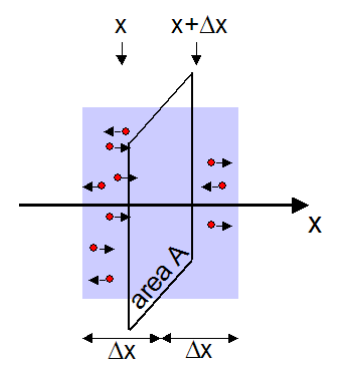
\includegraphics[scale=0.7]{Figures/ficks_diffusion_law.png}
    \caption{Τυχαία κίνηση σωματιδίων σε μία διάσταση, διερχόμενα από επιφάνεια $A$.}
    \label{fig:ficks_diffusion_law}
\end{figure}

Η διάδοση ενέργειας με ακτινοβολία μπορεί να προσεγγιστεί ως μια διαδικασία διάχυσης (diffusion) όπως θα δείξουμε. Έστω μοναδιαία επιφάνεια και σωματίδια (π.χ. φωτόνια) τα οποία διέρχονται διαμέσου αυτής της επιφάνειας κατά μία διεύθυνση $x$ (στην περίπτωσή μας αυτή η διεύθυνση θα ήταν η ακτινική και το $\Delta x = \ell$), όπως φαίνεται στο σχήμα \ref{fig:ficks_diffusion_law}. Αριστερά της επιφάνειας η αριθμητική πυκνότητα των σωματιδίων είναι $n(x)$ και δεξιά $n(x+\Delta x)$. Υποθέτοντας ότι οι ταχύτητες στις τρεις διευθύνσεις του χώρου είναι κατανεμημένες ισοτροπικά ώστε $u_x = u_y = u_z$, προκύπτει ότι για μία από τις τρεις διευθύνσεις, $u_x = \frac{1}{3} \langle u \rangle$. Το ερώτημα είναι πόσα σωματίδια διέρχονται από την επιφάνεια $A$. Διαστασιακά, η ροή των σωματιδίων μπορεί να γραφτεί ως $F = n \,u$, και επειδή τα σωματίδια έχουν την ίδια πιθανότητα να κινούνται είτε προς τα αριστερά είτε προς τα δεξιά, τα μισά σωματίδια θα κινούνται προς τη μία κατεύθυνση και τα άλλα μισά προς την άλλη. Έτσι, η ροή για τα σωματίδια που κινούνται διαμέσου της επιφάνειας $A$, από τα αριστερά προς τα δεξιά θα είναι
\begin{equation*}
    F(x) = \frac{1}{2} n(x) \,\frac{1}{3} \langle u \rangle = \frac{1}{6} n(x) \,\langle u \rangle
\end{equation*}
Αντίστοιχα, η ροή των σωματιδίων που κινούνται διαμέσου της επιφάνειας $A$, από τα δεξιά προς τα αριστερά θα είναι
\begin{equation*}
    F(x + \Delta x) = \frac{1}{6} n(x+\Delta x) \,\langle u \rangle
\end{equation*}
Έτσι, η θετική (net) ροή θα είναι
\begin{equation*}
    F = \frac{1}{6} \langle u \rangle \left[ n(x+\Delta x) - n(x) \right]
\end{equation*}
Επειδή οι αριθμοί $n(x), \,n(x + \Delta x)$ δεν είναι σταθεροί αλλά μεταβάλλονται ανάλογα με τον αριθμό των σωματιδίων που διαπερνούν την επιφάνεια και καταλήγουν είτε αριστερά είτε δεξιά, η τελευταία σχέση γράφεται
\begin{align}
    \nonumber F &= \frac{1}{6} \langle u \rangle \left[ n - \frac{dn}{dx}\Delta x - \left( n + \frac{dn}{dx}\Delta x \right) \right] = - \frac{1}{3} \langle u \rangle \Delta x \frac{dn}{dx} \Rightarrow \\ \nonumber \\
    &\Rightarrow F = -D \frac{dn}{dx}
\end{align}
όπου ο συντελεστής $D = \frac{1}{3} \langle u \rangle \Delta x$ ονομάζεται "διαχυσιμότητα" (diffusivity) και αποτελεί μέτρο του ρυθμού με τον οποίο τα σωματίδια διασκορπίζονται. Το παραπάνω αποτέλεσμα γενικεύεται στις τρεις διαστάσεις
\begin{equation}
    \label{eq:ficks_diffusion_law}
    F = - D \nabla n
\end{equation}
και είναι γνωστό ως \textbf{νόμος διάχυσης του Fick}.

Αντί της αριθμητικής πυκνότητας $n$, μπορούμε να γράψουμε κατά αντιστοιχία ότι η ροή ενέργειας λόγω διάχυσης είναι
\begin{equation}
    \label{eq:energy_density_diffusion}
    F = -D \nabla u \xrightarrow{1D} F = -D \frac{du}{dr}
\end{equation}
όπου $u$ η πυκνότητα ενέργειας. Χρησιμοποιοώντας τον κανόνα αλυσίδας $\frac{du}{dT} \,\frac{dT}{dr}$, μπορούμε να γράψουμε την σχέση \eqref{eq:energy_density_diffusion} ως
\begin{equation}
    \label{eq:temperature_gradient_diffusion_law}
    F = -D \underbrace{\frac{du}{dT}}_{= \,C_{\text{V}}} \,\frac{dT}{dr} = - K\frac{dT}{dr} \xrightarrow{3D} \boxed{F = -K \nabla T}
\end{equation}
όπου ο συντελεστής 
\begin{equation}
    \label{eq:conductivity_diffusion_coefficient}
    K = \frac{1}{3} \langle u \rangle \ell C_{\text{V}} = \frac{1}{3 \kappa_\nu \rho} \langle u \rangle C_{\text{V}}
\end{equation}
ονομάζεται "αγωγιμότητα" (conductivity) και 
\begin{equation}
    \label{eq:specific_heat_capacity}
    C_{\text{V}} = \left( \frac{du}{dT} \right)_{\text{V}}
\end{equation}
η ειδική θερμοχωρητικότητα (specific heat capacity). Αυτή η περιγραφή ισχύει για όλα τα σωματίδια σε τοπική θερμοδυναμική ισορροπία, συμπεριλαμβανομένων και των φωτονίων. 

Για ένα αέριο φωτονίων, μπορούμε να θέσουμε $\langle u \rangle = c$, όπου $c$ η ταχύτητα του φωτός στο κενό. Η πυκνότητα ενέργειας δίνεται από τη σχέση \eqref{eq:photon_energy_density} και άρα η ειδική θερμοχωρητικότητα είναι
\begin{equation*}
    C_{\text{V}} = \left( \frac{du}{dT} \right)_{\text{V}} = 4 \alpha T^3
\end{equation*}
ενώ η μέση ελεύθερη διαδρομή σχετίζεται με την αδιαφάνεια μέσω της σχέσης \eqref{eq:mean_free_path}, όπου αν πάρουμε την μέση τιμή για όλες τις συχνότητες ($\langle \kappa \rangle \equiv \kappa$) μπορεί να γραφτεί
\begin{equation*}
    \ell_{\text{ph}} = \frac{1}{\kappa \rho}
\end{equation*}
Συνδυάζοντας όλα τα παραπάνω, μπορούμε να γράψουμε τον \textbf{συντελεστή αγωγιμότητας ακτινοβολίας} \eqref{eq:conductivity_diffusion_coefficient} ως
\begin{equation}
    \label{eq:radiation_conductivity_coefficient}
    K_{\text{rad}} = \frac{4}{3} \frac{\alpha \,c \,T^3}{\kappa \rho}
\end{equation}

Σε αυτό το σημείο αξίζει να αναφέρουμε ότι και η διάδοση ενέργειας μέσω αγωγής μπορεί να περιγραφεί ως μία διαδικασία διάχυσης με την ίδια συναρτησιακή μορφή της σχέσης \eqref{eq:temperature_gradient_diffusion_law} ώστε η συνδυαστική ροή ενέργειας να είναι
\begin{equation}
    \label{eq:radiative_and_conduction_flux}
    F = - \frac{4\alpha c T^3}{3\rho}\left( \frac{1}{\kappa_{\text{rad}}} + \frac{1}{\kappa_{\text{cd}}} \right) \nabla T
\end{equation}
όπου ορίσαμε την \textbf{αδιαφάνεια αγωγής}, $\kappa_{\text{cd}}$, σε αναλογία με την αδιαφάνεια ακτινοβολίας $\kappa_{\text{rad}}$. Αυτό το αποτέλεσμα σημαίνει απλά ότι ο μηχανισμός διάδοσης ενέργειας με τη μεγαλύτερη ροή θα είναι ο κυριάρχος, ή με άλλα λόγια, ο μηχανισμός για τον οποίο η αστρική ύλη παρουσιάζει τη μεγαλύτερη διαφάνεια.

Για έναν σφαιρικά συμμετρικό αστέρα, η τοπική λαμπρότητα σχετίζεται με την ροή μέσω της σχέσης 
$$F = \frac{l}{4\pi r^2}$$
και άρα η εξίσωση \eqref{eq:radiative_and_conduction_flux} γράφεται
\begin{align}
    \label{eq:energy_transport_radiation_eulerian_diff}
    \nonumber F_{\text{rad}} &= - \frac{4}{3} \frac{\alpha \,c \,T^3}{\kappa_{\text{rad}} \rho} \frac{dT}{dr} = \frac{l}{4\pi r^2} \Rightarrow \\ \nonumber \\
    &\Rightarrow \boxed{\frac{dT}{dr} = - \frac{3\kappa \rho}{16 \pi \alpha c T^3} \frac{l}{r^2}}
\end{align}
ή στο σύστημα συντεταγμένων του Lagrange
\begin{equation}
    \label{eq:energy_transport_radiation_lagrangian_diff}
    \boxed{\frac{dT}{dm} = - \frac{3}{64\pi^2 \alpha c} \frac{\kappa l}{r^4 T^3}}
\end{equation}
Αυτή είναι η θερμοβαθμίδα που απαιτείται ώστε όλη η λαμπρότητα $l$ να μεταφερθεί μέσω ακτινοβολίας και αποτελεί την τέταρτη διαφορική εξίσωση που περιγράφει τη δομή ενός αστέρα στην περίπτωση που έχουμε διάδοση ενέργειας μόνο μέσω ακτινοβολίας. Ένα αστέρι ή μια περιοχή ενός αστεριού στην οποία ισχύει αυτή η εξίσωση ονομάζεται ζώνη ακτινοβολίας (radiative).

Η εξίσωση \eqref{eq:energy_transport_radiation_lagrangian_diff} ισχύει όσο $\ell_{\text{ph}} \ll R$, δηλαδή όσο υπάρχει τοπική θερμοδυναμική ισορροπία. Αυτή η συνθήκη σταματάει να ισχύει όσο πλησιάζουμε την επιφάνεια του αστέρα, την φωτόσφαιρα, από την οποία διαφεύγουν φωτόνια ($\ell_{\text{ph}} \gtrsim R$). Κοντά στην φωτόσφαιρα, η προσέγγιση της διάχυσης παύει να ισχύει και πρέπει να λύσουμε την --πολύ πιο δύσκολη-- εξίσωση μεταφοράς. Ευτυχώς, συνθήκες τοπικής θερμοδυναμικής ισορροπίας και η προσέγγιση της διάχυσης ισχύουν σχεδόν για όλο το εσωτερικό των αστέρων.

Για έναν αστέρα που βρίσκεται σε υδροστατική ισορροπία, μπορούμε συνδυάζοντας τις εξισώσεις \eqref{eq:hydrostatic_equilibrium_lagrangian_coordinate} και \eqref{eq:energy_transport_radiation_lagrangian_diff} να γράψουμε την θερμοβαθμίδα ως
\begin{equation*}
    \frac{dT}{dm} = \frac{dP}{dm} \,\frac{dT}{dP} = - \frac{Gm}{4\pi r^4} \,\frac{T}{P} \,\frac{d\log T}{d\log P}
\end{equation*}
ώστε να ορίσουμε την αδιάστατη θερμοβαθμίδα ακτινοβολίας (radiative temperature gradient)
\begin{eqnarray}
    \label{eq:radiative_temperature_gradient}
    \nabla_{\text{rad}} = \left(\frac{d\log T}{d\log P} \right)_{\text{rad}} = \frac{3}{16\pi \alpha c G} \frac{\kappa l P}{m T^4}
\end{eqnarray}
Η σχέση \eqref{eq:radiative_temperature_gradient} περιγράφει την λογαριθμική μεταβολή της θερμοκρασίας με το βάθος (όπου το βάθος είναι εκφρασμένο μέσω της πίεσης) σε έναν αστέρα σε υδροστατική ισορροπία, αν η ενέργεια μεταφέρεται μόνο μέσω ακτινοβολίας.
%% ---------------------------------------------------------------------------------------------------- %%
%% ---------------------------------------------------------------------------------------------------- %%
%% ---------------------------------------------------------------------------------------------------- %%
\subsubsection{Η αδιαφάνεια στο εσωτερικό των αστέρων}
Οι εξισώσεις που περιγράφουν την διάχυση της ακτινοβολίας είναι ανεξάρτητες της συχνότητας $\nu$, αφού η ροή $F$ ολοκληρώνεται ως προς όλες τις συχνότητες. Γενικά όμως, ο συντελεστής αδιαφάνειας $\kappa_\nu$ εξαρτάται από την συχνότητα, οπότε η ποσότητα $\kappa$ που εμφανίζεται στην σχέση \eqref{eq:energy_transport_radiation_lagrangian_diff}
πρέπει να παριστάνει έναν μέσο όρο ως προς τη συχνότητα.

Αν με $F_\nu d\nu$ θεωρήσουμε την ροή ακτινοβολίας στο διάστημα συχνοτήτων $[\nu, \nu+d\nu]$, τότε η εξίσωση \eqref{eq:ficks_diffusion_law} πρέπει να αντικατασταθεί με
\begin{equation}
    \label{eq:ficks_diffusion_law_frequency_dependent}
    F_\nu = -D_\nu \nabla u_\nu = -D_\nu \frac{\partial u_\nu}{\partial T} \nabla T
\end{equation}
όπου $D_\nu = \frac{1}{3} c l_{\text{ph}} = \frac{c}{3 \kappa_nu \rho}$.  Επειδή θεωρούμε ότι η ακτινοβολία βρίσκεται σε θερμική ισορροπία με το αέριο, η πυκνότητα ενέργειας στο ίδιο διάστημα, συνδέεται με την ένταση της ακτινοβολίας που δίνεται από τον νόμο του Planck μεσω της σχέσης
\begin{equation}
    \label{eq:energy_density_intensity_correlation}
    B_\nu (T) = \frac{u_\nu (T) \,c}{4\pi}
\end{equation}
Η ολική ροή προκύπτει από την ολοκλήρωση της σχέσης \eqref{eq:ficks_diffusion_law_frequency_dependent} σε όλες τις συχνότητες
\begin{equation*}
    F = - \left[\frac{c}{3 \rho} \int_{0}^{\infty} \frac{1}{\kappa_\nu} \frac{\partial u_{\nu}}{\partial T} d\nu \right] \nabla T
\end{equation*}
η οποία έχει την ίδια μορφή με τη σχέση \eqref{eq:temperature_gradient_diffusion_law} όπου 
\begin{equation*}
    K_{\text{rad}} = \frac{c}{3 \rho} \int_{0}^{\infty} \frac{1}{\kappa_\nu} \frac{\partial u_{\nu}}{\partial T} d\nu
\end{equation*}
Συγκρίνοντας το παραπάνω αποτέλεσμα με τη σχέση \eqref{eq:radiation_conductivity_coefficient} καταλήγουμε ότι
\begin{equation}
    \frac{1}{\kappa} = \frac{1}{4\alpha T^3} \int_{0}^{\infty} \frac{1}{\kappa_\nu} \frac{\partial u_{\nu}}{\partial T} d\nu
\end{equation}
όπου ο παράγοντας $4 \alpha T^3$ ισούται με $\int_{0}^{\infty} \frac{\partial u_\nu}{\partial T} d\nu$ ώστε η παραπάνω σχέση να γράφεται γενικά
\begin{equation}
    \label{eq:rosseland_mean_opacity_energy_density}
    \frac{1}{\kappa} = \frac{\int_{0}^{\infty} \frac{1}{\kappa_\nu} \frac{\partial u_{\nu}}{\partial T} d\nu}{\int_{0}^{\infty} \frac{\partial u_\nu}{\partial T} d\nu}
\end{equation}
Η ποσότητα $\kappa$ ονομάζεται \textbf{μέση αδιαφάνεια κατά Rosseland} και είναι η αρμονική μέση τιμή της αδιαφάνεια ενός αερίου συγκεκριμένης σύστασης, θερμοκρασίας και πυκνότητας, ως προς όλες τις συχνότητες της ακτινοβολίας που απορροφάται ή σκεδάζεται (σταθμισμένη με στατιστικό βάρος τη συνάρτηση $\partial u_\nu / \partial T$). Συχνά η μέση αδιαφάνεια κατά Rosseland εμφανίζεται με τον όρο της έντασης της ακτινοβολίας αντί της πυκνότητας ενέργειας, ώστε χρησιμοποιώντας την σχέση \eqref{eq:energy_density_intensity_correlation} να γράφεται και
\begin{equation*}
    \frac{1}{\kappa} = \frac{\pi}{\alpha c T^3} \int_{0}^{\infty} \frac{1}{\kappa_\nu} \frac{\partial B_{\nu} (T)}{\partial T} d\nu
\end{equation*}
ή γενικά

\begin{equation}
    \label{eq:rosseland_mean_opacity_intensity}
    \boxed{\frac{1}{\kappa} \int_{0}^{\infty} \frac{\partial B_{\nu} (T)}{\partial T} d\nu = \int_{0}^{\infty} \frac{1}{\kappa_\nu} \frac{\partial B_{\nu} (T)}{\partial T} d\nu}
\end{equation}

Όταν μελετάμε το εσωτερικό των αστέρων, δεν ενδιαφερόμαστε ιδιαίτερα για την ειδική ένταση $I_\nu$ (και την αντίστοιχη λαμπρότητα $L_\nu$), αφού δεν είναι δυνατόν να παρατηρήσουμε την κατανομή της λαμπρότητας με τη συχνότητα. Αντίθετα, ενδιαφερόμαστε για την ολική λαμπρότητα, $L$, η οποία συνδέεται άμεσα με το ενεργειακό ισοζύγιο του αστέρα (αφού σε κατάσταση ισορροπίας, η ενέργεια που ακτινοβολείται ως λαμπρότητα αναπληρώνεται από τις πηγές ενέργειας του αστέρα). Η μέση αδιαφάνεια κατά Rosseland είναι χρήσιμη όταν θέλουμε να υπολογίσουμε τη συνολική ενέργεια που απορροφήθηκε σε όλα τα μήκη κύματος, κάτι που απαιτείται στους υπολογισμούς της αστρικής δομής.


Ο συντελεστής αδιαφάνειας στο εσωτερικό των αστέρων οφείλεται στους μηχανισμούς που περιγράψαμε στο Κεφάλαιο \ref{ch:Chapter4}, δηλαδή σε φωτοϊονισμό (bound-free transition), σε πέδηση (free-free transition) ή σε σκεδάσεις (Thomson και Compton). Ο συντελεστής αδιαφάνειας που οφείλεται σε σκεδάσεις φωτονίων από ηλεκτρόνια, $\kappa_{\text{scat}}$, αποδεικνύεται ότι εξαρτάται μόνο από τη χημική σύσταστη της ύλης του αστέρα, και δίνεται από τη σχέση
\begin{equation}
    \label{eq:opacity_scattering}
    \kappa_{\text{scat}} = 0.2 (1+X) \,\text{cm$^2$/gr}
\end{equation}
όπου $X$ είναι η περιεκτικότητα της ύλης σε υδρογόνο. Παρατηρούμε ότι ο συντελεστής απορρόφησης λόγω σκέδασης από ηλεκτρόνια είναι ανεξάρτητος από τη συχνότητα των φωτονίων.

Οι συντελεστές απορρόφησης των δύο άλλων μηχανισμών, $\kappa_{\nu}^{\text{bf}}$ και $\kappa_{\nu}^{\text{ff}}$, είναι συναρτήσεις \textit{και} της συχνότητας, και επομένως χρειαζόμαστε τις αντίστοιχες αδιαφάνειες κατά Rosseland, $\kappa_{\text{bf}}$ και $\kappa_{\text{ff}}$. Αυτές έχουν υπολογιστεί από τον Kramer και δίνονται από τις σχέσεις
\begin{align}
    \kappa_{\text{bf}} &= a(X,Z,g_a,t) \rho T^s \label{eq:opacity_bound_free} \\ \nonumber \\
    \kappa_{\text{ff}} &= b(X,Z,g_b) \rho T^s \label{eq:opacity_free_free}
\end{align}
όπου ο εκθέτης, $s$, είναι συνάρτηση της θεμοκρασίας. Για τις υψηλές θερμοκρασίες που επικρατούν στο εσωτερικό των αστέρων ($T \geq 10^5$) αποδεικνύεται ότι $s = -3.5$, ενώ για σχετικά χαμηλές θερμοκρασίες ($T \approx 10^4$) αποδεικνύεται ότι $s = 10$. Οι συναρτήσεις $a, b$, στην περίπτωση που $s=-3.5$, ορίζονται από τις σχέσεις
\begin{align}
    a &= 4.34 \times 10^{25} \,\frac{g_a}{t} Z(1 + X) \label{eq:gaunt_factor_bf} \\ \nonumber \\
    b &= 3.68 \times 10^{22} \,g_b (1 + X) (1 - Z) \label{eq:gaunt_factor_ff}
\end{align}
Στις παραπάνω σχέσεις, οι συντελεστές $g_a, g_b$ και $t$ ονομάζονται \textbf{συντελεστές Gaunt} και \textbf{συντελεστής αποκοπής} (guillotine factor) αντίστοιχα. Οι συντελεστές Gaunt διορθώνουν τις αποκλίσεις μεταξύ της κλασικής και κβαντομηχανικής λύσης, ενώ ο συντελεστής αποκοπής διορθώνει τα σφάλματα των προσεγγίσεων κατά τον υπολογισμό της σχέσης \eqref{eq:gaunt_factor_bf}. Συνηθισμένες τιμές για τους συντελεστές αυτούς είναι $g_a \approx g_b \approx 3$ και $t \approx 10$. Το $X$ αντιπροσωπεύει την περιεκτικότητα (κατά μάζα) της ύλης του αστέρα σε υδρογόνο και το $Z$ την περιεκτικότητα της ύλης του αστέρα σε στοιχεία βαρύτερα από το ήλιο ("μέταλλα"), γι΄ αυτό και ονομάζεται και "metallicity".

Είθισται, οποιαδήποτε σχέση για την αδιαφάνεια έχει τη μορφή
\begin{equation}
    \label{eq:kramers_opacity_law_form}
    \kappa \propto \rho T^{-7/2}
\end{equation}
να ονομάζεται \textbf{αδιαφάνεια κατά Kramer}.

Από τους ορισμούς των $\kappa_{\text{bf}}, \kappa_{\text{ff}}$ παρατηρούμε ότι η αδιαφάνεια κατά Kramer είναι φθίνουσα συνάρτητη της θερμοκρασίας. Έτσι, σε αρκετά μεγάλες θερμοκρασίες ($T > 10^8 \,\text{K}$) η τιμή της τείνει στο μηδέν και επομένως γίνεται μικρότερη από την αδιαφάνεια σκέδασης απο ηλεκτρόνια $\kappa_{\text{scat}}$ (που είναι ανεξάρτητη της θερμοκρασίας). Από το αποτέλεσμα αυτό συμπεραίνουμε ότι η αδιαφάνεια κατά Kramer (μηχανισμοί bound-free και free-free) κυριαρχεί στους (ψυχρότερους) αστέρες μεταγενέστερων φασματικών τύπων, ενώ η αδιαφάνεια σκέδασης από ηλεκτρόνια κυριαρχεί στους (θερμότερους) αστέρες των προγενέστερων φασματικών τύπων.
%% ---------------------------------------------------------------------------------------------------- %%
%% ---------------------------------------------------------------------------------------------------- %%
%% ---------------------------------------------------------------------------------------------------- %%
\subsubsection{Το όριο Eddington}
Είδαμε ότι η διάδοση ενέργειας μέσω ακτινοβολίας μέσα σε έναν αστέρα απαιτεί μία θερμοβαθμίδα $dT/dr$, το μέγεθος της οποίας δίνεται από την εξίσωση \eqref{eq:energy_transport_radiation_eulerian_diff}. Η πίεση της ακτινοβολίας δίνεται από τη σχέση \eqref{eq:radiation_pressure_black_body} και άρα η βαθμίδα της πίεσης της ακτινοβολίας είναι
\begin{equation}
    \label{eq:radiation_pressure_gradient}
    \frac{dP_{\text{rad}}}{dr} = \frac{4}{3} \alpha T^3 \,\frac{dT}{dr} = - \frac{\kappa \rho}{4\pi c} \frac{l}{r^2}
\end{equation}
Αυτή η πίεση της ακτινοβολίας παριστάνει μία δύναμη που ασκείται προς το εξωτερικό του αστέρα λόγω της ροής των φωτονίων προς αυτή την κατεύθυνση. Φυσικά, για έναν αστέρα που βρίσκεται σε υδροστατική ισορροπία, αυτή η δύναμη πρέπει να είναι μικρότερη από τη δύναμη της βαρύτητας, όπως αυτή δίνεται από τη βαθμίδα της πίεσης που είναι απαραίτητη για την εδραίωση της υδροστατικής ισορροπίας (σχέση \ref{eq:hydrostatic_equilibrium_eulerian coordinates}). Αυτό σημαίνει ότι
\begin{align}
    \label{eq:eddington_limit}
    \nonumber \left| \frac{dP_{\text{rad}}}{dr} \right| &< \left| \left( \frac{dP}{dr} \right)_{\text{HE}} \right| \Rightarrow \frac{\kappa \rho}{4 \pi c} \frac{l}{r^2} < \frac{G m \rho}{r^2} \\ \nonumber \\
    &\Rightarrow l < \frac{4\pi G m c}{\kappa} = l_{\text{Edd}}
\end{align}
Η ποσότητα $l_{\text{Edd}} = \frac{4\pi G m c}{\kappa}$ ονομάζεται (τοπική) \textbf{λαμπρότητα Eddington} και παριστάνει τη μέγιστη λαμπρότητα που μπορεί να μεταφερθεί από την ακτινοβολία σε έναν αστέρα που βρίσκεται σε υδροστατική ισορροπία.

Το όριο Eddington που παριστάνεται από την ανισότητα \eqref{eq:eddington_limit} μπορεί να παραβιαστεί σε περιπτώσεις πολύ μεγάλων ροών θερμότητας (μεγάλα $l$), οι οποίες προκαλούνται από έντονη "καύση" των πυρηνικών καυσίμων, ή από πολύ μεγάλες αδιαφάνειες $\kappa$. Όπως αναφέραμε παραπάνω, υψηλές τιμές αδιαφάνειας εμφανίζονται σε σχετικά χαμηλές θερμοκρασίες, κοντά στην θερμοκρασία ιονισμού του υδρογόνου και του ηλίου (π.χ. εξωτερικά στρώματα του Ήλιου). Σε αυτές τις περιπτώσεις, η υδροστατική ισορροπία (σχέση \ref{eq:hydrostatic_equilibrium_eulerian coordinates}) και η ισορροπία λόγω της μεταφοράς ενέργειας με ακτινοβολία (radiative equilibrium, σχέση \ref{eq:energy_transport_radiation_eulerian_diff}) δεν μπορούν να ισχύουν ταυτόχρονα. Γι' αυτό, προκειμένου ο αστέρας να παραμείνει σε υδροστατική ισορροπία, η ενέργεια πρέπει να μεταφερθεί με άλλον τρόπο εκτός της διάχυσης ακτινοβολίας. Αυτός ο τρόπος είναι μέσω ρευμάτων μεταφοράς που θα αναλύσουμε παρακάτω. Ισχύει ότι η ανισότητα \eqref{eq:eddington_limit} είναι αναγκαία, αλλά όχι ικανή συνθήκη για μία ζώνη ενός αστέρα να είναι σταθερή ενάντια στα ρεύματα μεταφοράς.

Τα επιφανειακά στρώματα ενός αστέρα διαδίδουν πάντα την ενέργεια μέσω ακτινοβολίας αφού είναι εκείνη η περιοχή από την οποία η ενέργεια διαφεύγει με τη μορφή φωτονίων. Εφαρμόζοντας τη σχέση \eqref{eq:eddington_limit} στην επιφάνεια του αστέρα όπου $m=M$ προκύπτει
\begin{equation}
    \label{eq:eddington_surface_limit}
    L < L_{\text{Edd}} = \frac{4\pi G M c}{\kappa} 
\end{equation}
όπου $\kappa$ είναι η αδιαφάνεια της φωτόσφαιρας. Η λαμπρότητα Eddington που δίνεται από την σχέση \eqref{eq:eddington_surface_limit} είναι μία κριτική τιμή λαμπρότητας που δεν μπορεί να ξεπεραστεί από έναν αστέρα σε υδροστατική ισορροπία. Παραβίαση αυτής της συνθήκης σημαίνει παραβίαση της υδροστατικής ισορροπίας: η ύλη εκδιώχνεται από τον αστέρα λόγω της πίεσης της ακτινοβολίας, οδηγώντας σε βίαιη απώλεια μάζας. Όπως είδαμε και παραπάνω, σε περιοχές που κυριαρχεί η σκέδαση φωτονίων από ηλεκτρόνια, η αδιαφάνεια είναι σχεδόν σταθερή και άρα η λαμπρότητα Eddington εξαρτάται μόνο από τη μάζα
\begin{equation}
    \label{eq:eddington_luminosity_electron_scattering_opacity}
    L_{\text{Edd}} = \frac{4\pi G M c}{0.2 (1+X)} = \frac{2.52 \times 10^{38}}{1+X} \left( \frac{M}{M_\odot} \right) \,\text{erg/s}
\end{equation}

Επειδή η $L_{\text{Edd}}$ είναι ανάλογη της μάζας $m$, ενώ οι αστέρες της κύριας ακολουθίας ακολουθούν μία σχέση λαμπρότητας-μάζας (Κεφάλαιο \ref{ch:Chapter2}) $L \propto M^x,  \,x>1$, αυτό σημαίνει ότι όσο αυξάνεται η μάζα των αστέρων κάποια στιγμή η λαμπρότητά τους θα ξεπεράσει το όριο Eddington. Άρα, περιμένουμε να υπάρχει κάποιο ανώτερο όριο στη μάζα που μπορούν να έχουν οι αστέρες, το οποίο βρίσκεται με απαλοιφή της λαμπρότητας από τις δύο παραπάνω σχέσεις.

Υιοθετώντας μία σχέση λαμπρότητας-μάζας
\begin{equation}
    \label{eq:observed_mass_luminosity_relation}
    \frac{L}{L_\odot} = 3.013 \left( \frac{M}{M_\odot} \right)^{2.91}
\end{equation}
από τις σχέσεις \eqref{eq:eddington_luminosity_electron_scattering_opacity} και \eqref{eq:observed_mass_luminosity_relation} προκύπτει ότι
\begin{align*}
    11.54 &\times 10^{33} \left( \frac{M}{M_\odot} \right)^{2.91} = \frac{2.52 \times 10^{38}}{1+X} \left( \frac{M}{M_\odot} \right) \Rightarrow \\\\
    &\Rightarrow \left( \frac{M}{M_\odot} \right)^{1.91} = \frac{2.16 \times 10^4}{1+X} \Rightarrow \\\\
    &\Rightarrow M_{\text{max}} = \left(\frac{2.16 \times 10^4}{1+X} \right)^{0.524} \,M_\odot
\end{align*}
Για μία χημική σύσταση με 70\,\% υδρογόνο ($X=1$), έχουμε ότι
\begin{equation}
    M_{\text{max}} \simeq 140 \,M_{\odot}
\end{equation}
τιμή η οποία είναι συμβατή με τις μέχρι τώρα παρατηρήσεις καθώς δεν έχουμε εντοπίσει αστέρες με μάζα μεγαλύτερη των $100 \,M_\odot$.
%% ---------------------------------------------------------------------------------------------------- %%
%% ---------------------------------------------------------------------------------------------------- %%
%% ---------------------------------------------------------------------------------------------------- %%
\subsubsection{Σχέσεις λαμπρότητας-μάζας}
Είδαμε ότι τα φωτόνια που εκπέμπονται από τις πυρηνικές αντιδράσεις που λαμβάνουν χώρα στον πυρήνα ενός αστέρα, απορροφούνται σχεδόν αμέσως και επανεκπέμπονται σε μεγαλύτερα μήκη κύματος\footnote{ Η διαφορά ενέργειας μεταξύ του φωτονίου που απορροφήθηκε και αυτού που εκπέμφθηκε πήγε στην θέρμανση του υλικού.} από ανώτερα στρώματα προς τυχαίες διευθύνσεις, μία διαδικασία που ονομάζεται "\textbf{τυχαίος βηματισμός}" (random walk) και μπορεί να θεωρηθεί ως μια διαδικασία διάχυσης της ακτινοβολίας. Από τη θεωρία του τυχαίου βηματισμού γνωρίζουμε ότι τα βήματα που απαιτούνται για να καλύψει ένα φωτόνιο μία μέση απόσταση ίση με την ακτίνα του αστέρα είναι
\begin{equation}
    \label{eq:random_walk_steps}
    N = \left( \frac{R}{\ell_{\text{ph}}} \right)^2
\end{equation}
Αυτό συνεπάγεται ότι ο μέσος χρόνος που χρειάζονται τα φωτόνια για να διανύσουν απόσταση $\ell_{\text{ph}}$ λόγω διάχυσης είναι
\begin{equation}
    \label{eq:diffusion_time}
    t_{\text{diffusion}} = \frac{\ell_{\text{ph}}}{c} N = \frac{R^2}{\ell_{\text{ph}} c}
\end{equation}

Έστω τώρα ότι η ακτίνα του πυρήνα ενός αστέρα είναι κάποιο κλάσμα της συνολικής ακτίνας του αστέρα $R_c = fR, \,f<1$. Η πυκνότητα ενέργειας που παράγεται στον πυρήνα είναι $u=\alpha T_c^4$ και άρα η συνολική διαθέσιμη ενέργεια του πυρήνα είναι 
\begin{equation}
    E = \frac{4}{3} \pi R_c^3 \,\alpha T_c^4
\end{equation}

Σε πρώτη προσέγγιση, η μέση λαμπρότητα θα είναι τότε
\begin{equation}
    L \approx \frac{E_c}{t_{\text{diffusion}}} = \frac{\frac{4\pi}{3} (fR)^3 \alpha T_c^4}{\left( \frac{R^2}{\ell_{\text{ph}} c} \right)} \Rightarrow \boxed{ L \propto R \ell_{\text{ph}} T_c^4}
\end{equation}

Για να βρούμε μία σχέση $L = f(M)$, πρέπει να βρούμε σχέσεις που να συνδέεουν τις ποσότητες $R, \ell_{\text{ph}}, T_c$ με τη μάζα. Από τις σχέσεις \eqref{eq:mean_free_path}, \eqref{eq:lower_limit_of_central_pressure_for_stars_in_HE} έχουμε ότι
\begin{align*}
    \ell_{\text{ph}} &\propto \frac{1}{\langle \rho \rangle} \\\\
    \langle \rho \rangle &\propto \frac{M}{R^3} \\\\
    P_c &\propto \frac{M^2}{R^4}
\end{align*}

Έτσι, μπορούμε να διακρίνουμε τις εξής περιπτώσεις
\begin{itemize}
    \item Για αστέρες μεγάλης μάζας, $M>30M_\odot$, ο κυρίαρχος μηχανισμός πίεσης είναι η πίεση ακτινοβολίας $P_{\text{rad}} = \frac{1}{3} \alpha T_c^4$ και άρα
    \begin{equation*}
        P_c \propto \frac{M^2}{R^4} \propto T_c^4
    \end{equation*}
    Συνεπώς
    \begin{equation}
        \label{eq:high_mass_LM_relationship}
        L \propto R \frac{1}{\langle \rho \rangle} T_c^4 \Rightarrow \boxed{L \propto M}
    \end{equation}
    
    \item Για αστέρες ενδιάμεσης μάζας, $3M_\odot < M < 30M_\odot$, ισχύουν οι ίδιες σχέσεις με παραπάνω αλλά τώρα ο κυρίαρχος μηχανισμός πίεσης είναι η πίεση του αερίου $P_{\text{gas}} \propto \rho T_c$ και άρα
    \begin{equation*}
        P_c \propto \frac{M^2}{R^4} \propto \rho T_c \longrightarrow T_c \propto \frac{M^2}{R^4} \frac{1}{\langle \rho \rangle}
    \end{equation*}
    Συνεπώς
    \begin{equation}
        \label{eq:intermediate_mass_LM_relationship}
        L \propto R \frac{1}{\langle \rho \rangle} \left(\frac{M^2}{R^4} \frac{1}{\langle \rho \rangle} \right)^4 \Rightarrow \boxed{L \propto M^3}
    \end{equation}
\end{itemize}
%% ---------------------------------------------------------------------------------------------------- %%
%% ---------------------------------------------------------------------------------------------------- %%
%% ---------------------------------------------------------------------------------------------------- %%
\subsubsection{Διάδοση ακτινοβολίας με ρεύματα μεταφοράς}
Στην Αστροφυσική συχνά συναντάμε προβλήματα όπου ένα ρευστό θερμαίνεται από "κάτω" (π.χ. αστέρες, ατμόσφαιρα της Γης όπου ο Ήλιος θερμαίνει την επιφάνεια κτλ). Αυτό οδηγεί σε μια θερμοβαθμίδα: ζεστό στη βάση, πιο ψυχρό προς τα πάνω\footnote{Εδώ ο όρος "πάνω" θα αναφέρεται στην αντίθετη κατεύθυνση από αυτή της βαρύτητας.}. Αν η θερμοβαθμίδα γίνει πολύ μεγάλη, το αέριο αναπτύσσει ένα είδος αστάθειας (convective instability) ώστε "φυσαλίδες" αερίου που είναι πιο θερμές από το περιβάλλον στο οποίο βρίσκονται, μετακινούνται προς τα ανώτερα στρώματα μέχρι να διασκορπίσουν (dissipate) την περίσσεια θερμική ενέργεια που κουβαλούν και να ενσωματωθούν στο καινούργιο περιβάλλον, υιοθετώντας όλες τις ιδιότητες που το χαρακτηρίζουν (πίεση, θερμοκρασία κτλ). 

Έστω ένα στοιχειώδες κομμάτι αερίου με πυκνότητα $\rho_b$ και πίεση $P_b$ το οποίο βρίσκεται μέσα σε υλικό πυκνότητας $\rho$ και πίεσης $P$. Ας υποθέσουμε ότι λόγω κάποιων μικρών διαταραχών, το στοιχειώδες αυτό κομμάτι αερίου μετατοπίζεται προς τα επάνω κατά μία μικρή απόσταση $\delta z \equiv \delta r$. Μετά την μετατόπιση, το κομμάτι αερίου θα έχει συνθήκες ($\rho_b^{\star}, P_b^{\star}$) ενώ το καινούργιο του περιβάλλον θα χαρακτηρίζεται από συνθήκες ($\rho^{\prime}, P^{\prime}$), όπου
\begin{align}
    \rho^{\prime} &= \rho + \frac{d\rho}{dr} \delta r \label{eq:convection:density_perturbation} \\ \nonumber \\
    P^{\prime} &= P + \frac{dP}{dr} \delta r \label{eq:convection:pressure_perturbation}
\end{align}


\begin{figure}[t]
    \centering
    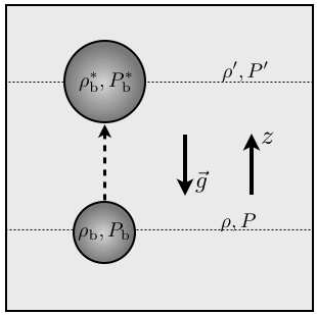
\includegraphics[scale=0.6]{Figures/convection_scheme.png}
    \caption{Σχηματική αναπαράσταση του κριτηρίου Schwarzschild ενάντια στην ύπαρξη ρευμάτων μεταφοράς. Ένα στοιχειώδες κομμάτι αερίου (blob) μετατοπίζεται προς την επιφάνεια του αστέρα όπου διαστέλλεται αδιαβατικά για να διατηρήσει μηχανική ισορροπία με το περιβάλλον του. Αν η πυκνότητα του στοιχειώδους κομματιού είναι μεγαλύτερη από την πυκνότητα του υλικού που το περιβάλλει, θα βυθιστεί πίσω στην αρχική του θέση. Αν όμως η πυκνότητά του είναι μικρότερη από την πυκνότητα του χώρου γύρω του, δυνάμεις άνωσης θα το επιταχύνουν προς τα επάνω και θα δημιουργηθεί ένα ρεύμα μεταφοράς.}
    \label{fig:convection_scheme}
\end{figure}

Αρχικά, το στοιχειώδες κομμάτι αερίου υποθέτουμε ότι βρισκόταν σε κατάσταση μηχανικής και θερμικής ισορροπίας με τον περιβάλλοντα χώρο, ώστε $\rho_b = \rho$ και $P_b = P$. Μετά την μετατόπιση, το κομμάτι πρέπει να επανέλθει σε μία νέα κατάσταση μηχανικής και θερμικής ισορροπίας. Γενικά, ο χρόνος που χρειάζεται για να εδραιώσει μία νέα κατάσταση μηχανικής ισορροπίας είναι ο δυναμικός χρόνος, $\tau_{\text{dyn}}$, ενώ η θερμική ισορροπία επέρχεται πολύ πιο αργά, στον θερμικό χρόνο $\tau_{\text{KH}}$. Επειδή ισχύει ότι $\tau_{\text{dyn}} \ll \tau_{\text{KH}}$, μπορούμε να υποθέσουμε ότι η μηχανική ισορροπία επέρχεται πριν προλάβει να γίνει ανταλλαγή θερμότητας με το περιβάλλον, ώστε η διαδικασία της μετατόπισης να είναι προσεγγιστικά αδιαβατική και να ισχύει $P_b^{\star} = P^{\prime}$ αλλά γενικά $\rho_b^{\star} \neq \rho^{\prime}$. Αυτό σημαίνει ότι η παραπάνω διαδικασία μπορεί να περιγραφεί από μία αδιαβατική καταστατική εξίσωση της μορφής $P \propto \rho^{\gamma}$, όπου $\gamma$ ο αδιαβατικός δείκτης. Έτσι, μπορούμε να γράψουμε

\begin{align*}
    \begin{cases}
        P_b &\propto \rho_b^{\gamma} \\
        P_b^{\star} &\propto {\rho_b^{\star}}^{\gamma}
    \end{cases} &\Rightarrow
    \frac{ P_b^{\star}}{P_b} \propto \left(\frac{\rho_b^{\star}}{\rho_b}\right)^{\gamma} \Rightarrow \rho_b^{\star} \propto \rho_b \left(\frac{P_b^{\star}}{P_b} \right)^{1/\gamma} \Rightarrow \\\\
    &\Rightarrow \rho_b^{\star} \propto \rho_b \left(\frac{P^{\prime}}{P} \right)^{1/\gamma} \xRightarrow{\eqref{eq:convection:pressure_perturbation}}{\rho_b^{\star} = \rho_b \left(1 + \frac{1}{P} \frac{dP}{dr}\delta r \right)^{1/\gamma}}
\end{align*}

Στο όριο των μικρών μετατοπίσεων $\delta r$, μπορούμε να χρησιμοποιήσουμε ανάπτυγμα Taylor για να δείξουμε ότι
\begin{eqnarray}
    \label{eq:convection:new_blob_density_expression}
    \rho_b^{\star} = \rho + \frac{\rho}{\gamma P} \frac{dP}{dr} \delta r
\end{eqnarray}
όπου χρησιμοποίησαμε την αρχική συνθήκη $\rho_b = \rho$, και ότι το ανάπτυγμα Taylor της συνάρτησης $f(x) = (1+x)^{1/\gamma}$ δίνεται προσεγγιστικά από $f(x) \simeq 1 + \frac{1}{\gamma}x + \dots$.

Έστω ένα στρωματοποιημένο (stratified) υλικό στο οποίο $d\rho/dr < 0$ και $dP/dr < 0 $. Σε αυτή την περίπτωση, εαν $\rho_b^{\star} > \rho^{\prime}$ τότε το στοιχειώδες κομμάτι αερίου είναι πιο βαρύ από τον περιβάλλοντα χώρο στον οποίο βρίσκεται και θα βυθιστεί στην αρχική του θέση. Τότε το σύστημα είναι σταθερό ως προς τη δημιουργία ρεύματος μεταφοράς. Αν όμως $\rho_b^{\star} < \rho^{\prime}$, τότε δημιουργείται αστάθεια καθώς δυνάμεις άνωσης θα το επιταχύνουν προς τα επάνω. Από τις σχέσεις \eqref{eq:convection:density_perturbation} και \eqref{eq:convection:new_blob_density_expression} προκύπτει ότι η ευστάθεια απαιτεί
\begin{equation}
    \label{eq:convection:schwarzschild_density_pressure}
    \rho_b^{\star} > \rho^{\prime} \Rightarrow \boxed{\frac{d\rho}{dr} < \frac{\rho}{\gamma P} \frac{dP}{dr}}
\end{equation}
ή ισοδύναμα, διαιρώντας με $dP/dr$ (το οποίο είναι αρνητικό)
\begin{equation}
    \label{eq:convection:schwarzschild_log_density_log_pressure}
    \boxed{\frac{d\log \rho}{d\log P} > \frac{1}{\gamma}}
\end{equation}
Η σχέση \eqref{eq:convection:schwarzschild_log_density_log_pressure} ονομάζεται \textbf{κριτήριο ευστάθειας Schwarzschid}, και αν παραβιαστεί τότε έχουμε την δημιουργία ρευμάτων μεταφοράς.

Παρόλα αυτά, οι σχέσεις \eqref{eq:convection:schwarzschild_density_pressure} και \eqref{eq:convection:schwarzschild_log_density_log_pressure} απαιτούν τον υπολογισμό βαθμίδας πυκνότητας που δεν είναι μέρος των διαφορικών εξισώσεων που περιγράφουν την αστρική δομή. Θα προτιμούσαμε να εκφράσουμε το κριτήριο του Schwarzschild με τη μορφή θερμοβαθμίδας, όπως αυτή εμφανίζεται στην εξίσωση μεταφοράς ενέργειας με ακτινοβολίας (σχέσεις \ref{eq:energy_transport_radiation_eulerian_diff} -- \ref{eq:radiative_temperature_gradient}).
Χρησιμοποιώντας ότι 
\begin{equation*}
    \rho = \rho(P,T) = \frac{\mu m_H}{kT}P
\end{equation*}
μπορούμε να δείξουμε οτι
\begin{align}
    \label{eq:convection:dRho_dr}
    \nonumber \frac{d\rho}{dr} &= \frac{\mu m_H}{k} \left(\frac{1}{T} \frac{dP}{dr} - \frac{P}{T^2}\frac{dT}{dr} \right) = \underbrace{\frac{\mu m_H}{kT}P}_{= \,\rho} \left(\frac{1}{P} \frac{dP}{dr} - \frac{1}{T} \frac{dT}{dr} \right) \Rightarrow \\\nonumber\\
    &\Rightarrow \frac{d\rho}{dr} = \frac{\rho}{P} \frac{dP}{dr} - \frac{\rho}{T} \frac{dT}{dr}
\end{align}
Από τις σχέσεις \eqref{eq:convection:density_perturbation} και \eqref{eq:convection:dRho_dr} προκύπτει ότι
\begin{align*}
    \rho^{\prime} &= \rho + \frac{d\rho}{dr} \delta r = \rho + \left(\frac{\rho}{P} \frac{dP}{dr} - \frac{\rho}{T} \frac{dT}{dr} \right)\delta r \Rightarrow \\\\
    &\Rightarrow \rho^{\prime} - \rho = \left(\frac{\rho}{P} \frac{dP}{dr} - \frac{\rho}{T} \frac{dT}{dr} \right)\delta r \xRightarrow{\eqref{eq:convection:new_blob_density_expression}} \\\\
    &\Rightarrow \rho^{\prime} - \rho_b^{\star} + \frac{\rho}{\gamma P} \frac{dP}{dr} \delta r = \left(\frac{\rho}{P} \frac{dP}{dr} - \frac{\rho}{T} \frac{dT}{dr} \right)\delta r \Rightarrow \\\\
    &\Rightarrow \rho_b^{\star} - \rho^{\prime} = \left(- \frac{\gamma - 1}{\gamma}\frac{\rho}{P} \frac{dP}{dr} + \frac{\rho}{T} \frac{dT}{dr} \right)\delta r
\end{align*}

Η ευστάθεια απαιτεί $\rho_b^{\star} - \rho^{\prime} > 0$, άρα αφού $dP/dr < 0$ και $dT/dr < 0$, θα έχουμε
\begin{align}
    \label{eq:convection:schwarzschild_criterion_dT_dr}
    \nonumber \rho_b^{\star} &- \rho^{\prime} > 0 \Rightarrow \left(- \frac{\gamma - 1}{\gamma}\frac{1}{P} \frac{dP}{dr} + \frac{1}{T} \frac{dT}{dr}\right) \rho \delta r > 0 \xRightarrow{\rho > 0, \delta r > 0} \\\nonumber \\
    \nonumber &\Rightarrow - \frac{\gamma - 1}{\gamma}\frac{1}{P} \frac{dP}{dr} + \frac{1}{T} \frac{dT}{dr} > 0 \Rightarrow \\\nonumber\\
    &\Rightarrow \boxed{\left| \frac{dT}{dr} \right| < \frac{\gamma - 1}{\gamma} \frac{T}{P} \left| \frac{dP}{dr}\right|}
\end{align}
Η τελευταία μορφή του κριτηρίου Schwarzschild μας δείχνει ότι όταν η θερμοβαθμίδα γίνει πολύ μεγάλη, τότε το σύστημα γίνεται ασταθές ως προς την εμφάνιση ρευμάτων μεταφοράς, και μαζί με την σχέση \eqref{eq:energy_transport_radiation_eulerian_diff} για την περίπτωση μεταφοράς ενέργειας με ακτινοβολία, αποτελεί την τέταρτη διαφορική εξίσωση που περιγράφει τη δομή ενός αστέρα (αν αντί για ανισότητα πάρουμε ισότητα), στην περίπτωση που έχουμε μεταφορά ενέργειας μέσω δινορευμάτων.

Παρόλα αυτά, υπάρχει ακόμα ένας τρόπος να γράψουμε το κριτήριο του Schwartzschild και η οποία θα μας επιτρέψει να αντιληφθούμε καλύτερα το πότε η μεταφορά ενέργειας μέσω δινορευμάτων υπερισχύει αυτής της ακτινοβολίας.
Γράφοντας την καταστατική εξίσωση σε διαφορική μορφή (δες Παράρτημα \ref{apx:kinetic_theory}), η διακύμανση της πυκνότητας ως προς την πίεση σε όλον τον αστέρα θα είναι
\begin{align}
    \label{eq:convection:dlogRho_dlogP_actual_temp_gradient}
    \nonumber \frac{dP}{P} &= \chi_\rho \frac{d\rho}{\rho} + \chi_T \frac{dT}{T} \Rightarrow \\\nonumber\\
    \nonumber &\Rightarrow d\log P = \chi_\rho d\log \rho + \chi_T d\log T \Rightarrow \\\nonumber\\
     &\Rightarrow \frac{d\log \rho}{d \log P} = \frac{1}{\chi_\rho} \left( 1 - \chi_T \nabla \right)
\end{align}
όπου χρησιμοποιήσαμε το γεγονός ότι $d\log P = dP/P$, $d\log \rho = d\rho/\rho$ και $d\log T = dT/T$. Η ποσότητα $\displaystyle \nabla = \frac{d\log T}{d \log P}$ ονομάζεται \textbf{πραγματική θερμοβαθμίδα} (actual temperature gradient).

Για μια αδιαβατική μεταβολή ($dT = 0$), ισχύει 
\begin{equation}
    \frac{dP}{P} = \underbrace{\chi_\rho}_{= \,\gamma} \frac{d\rho}{\rho} + \chi_T \frac{\cancelto{0}{dT}}{T} \Rightarrow \frac{dP}{P} = \gamma \frac{d\rho}{\rho} \Rightarrow \frac{d\log P}{d\log \rho} = \gamma 
\end{equation}
και άρα συνδυάζοντας το παραπάνω αποτέλεσμα με τη σχέση \eqref{eq:convection:dlogRho_dlogP_actual_temp_gradient}, μπορούμε να γράψουμε για το στοιχειώδες κομμάτι αερίου που μετατοπίστηκε ότι
\begin{equation}
    \label{eq:convection:nabla_ad}
    \frac{1}{\gamma} = \frac{1}{\chi_\rho} \left(1 - \chi_T \nabla_{\text{ad}} \right) \Rightarrow \nabla_{\text{ad}} = \frac{\gamma - \chi_\rho}{\gamma \chi_T}
\end{equation}
όπου η ποσότητα $\displaystyle \nabla_{\text{ad}} = \left(\frac{\partial \log T}{\partial \log P} \right)_{\text{ad}}$ είναι η \textbf{αδιαβατική θερμοβαθμίδα}. Επειδή για το ιδανικό αέριο ισχύει $\chi_{\rho} = \chi_T = 1$, έχουμε ότι
\begin{equation}
    \nabla_{\text{ad}} = \frac{\gamma - 1}{\gamma}
\end{equation}

Συνδυάζοντας όλα τα παραπάνω, η έκφραση του κριτηρίου Schwartzschild \eqref{eq:convection:schwarzschild_log_density_log_pressure} γράφεται
\begin{align}
    \label{eq:convection:schwartzscild_criterion_actual_temp_gradient}
    \nonumber \frac{d\log \rho}{d\log P} &> \frac{1}{\gamma} \Rightarrow \frac{1}{\chi_\rho} \left( 1 - \chi_T \nabla \right) > \frac{1}{\chi_\rho} \left(1 - \chi_T \nabla_{\text{ad}} \right) \\\nonumber\\
    \nonumber &\Rightarrow 1 - \chi_T \nabla > 1 - \chi_T \nabla_{\text{ad}} \Rightarrow \chi_T \nabla < \chi_T \nabla_{\text{ad}} \Rightarrow \\\nonumber\\
    &\Rightarrow \boxed{\nabla < \nabla_{\text{ad}}}
\end{align}

Αν όλη η ενέργεια μεταφέρεται μέσω ακτινοβολίας, τότε $\nabla = \nabla_{\text{rad}}$, όπως δίνεται από την σχέση \eqref{eq:radiative_temperature_gradient} και άρα καταλήγουμε στο ότι
\begin{equation}
    \label{eq:convection:schwarzschild_criterion_nabla_rad_nabla_ad}
    \boxed{\nabla_{\text{rad}} < \nabla_{\text{ad}}}
\end{equation}
Σημασία πρέπει να δοθεί στα διάφορα $\nabla$ σύμβολα που εμφανίζονται στις διάφορες μορφές του κριτηρίου Schwarzschild. Το $\nabla_{\text{rad}}$ παριστάνει την \textit{χωρική θερμοβαθμίδα}, ενώ το $\nabla_{\text{ad}}$ παριστάνει την μεταβολή της θερμοκρασίας σε ένα στοιχειώδες κομμάτι αερίου που υπόκειται σε μια μεταβολή πίεσης.

Σύμφωνα λοιπόν με το κριτήριο Schwarzschild, περιμένουμε να έχουμε μεταφορά ενέργειας μέσω δινορευμάτων εαν
\begin{equation*}
    \nabla_{\text{rad}} = \frac{3}{16\pi \alpha c G} \frac{\kappa l P}{m T^4} > \nabla_{\text{ad}}
\end{equation*}
Αυτό προϋποθέτει ένα από τα ακόλουθα
\begin{itemize}
    \item Μία μεγάλη τιμή του $\kappa$, δηλαδή έχουμε ρεύματα μεταφοράς σε περιοχές όπου η αδιαφάνεια είναι μεγάλη. Παραδείγματα τέτοιων περιοχών είναι τα εξωτερικά στρώματα του Ήλιου και άλλων ψυχρών αστέρων, καθώς η αδιαφάνεια αυξάνεται όσο μειώνεται η θερμοκρασία (δες αδιαφάνεια κατά Kramer). Αφού αστέρες χαμηλής μάζας (μεταγενέστερου φασματικού τύπου) είναι πιο ψυχροί από αστέρες μεγάλης μάζας (προγενέστερου φασματικού τύπου), περιμένουμε αστέρες χαμηλής μάζας να έχουν εξωτερικά στρώματα που εμφανίζουν δινορεύματα.
    
    \item Μία μεγάλη τιμή του $l/m$, δηλαδή περιοχές με μεγάλη ροή ενέργειας. Σύμφωνα με τη σχέση \eqref{eq:thermal_equilibrium_lagrangian_form}, προς τον πυρήνα έχουμε $l/m \approx E_{\text{nuc}}$, έτσι αστέρες που έχουν παραγωγή ενέργειας στο κέντρο τους αναμένεται να έχουν πυρήνες που εμφανίζουν δινορεύματα. Αυτό συμβαίνει σε αστέρες σχετικά μεγάλης μάζας. 
    
    \item Μία μικρή τιμή του $\nabla_{\text{ad}}$, κάτι που συμβαίνει σε περιοχές μερικού ιονισμού σε σχετικά χαμηλές θερμοκρασίες (partial ionization zones). Έτσι, ακόμα κι αν η αδιαφάνεια δεν είναι πολύ μεγάλη, τα στρώματα της επιφάνειας ενός αστέρα μπορεί να είναι ασταθή όσον αφορά την δημιουργία δινορευμάτων. Αποδεικνύεται ότι αστέρες ανεξαρτήτου μάζας έχουν ρηχές επιφανειακές περιοχές στις οποίες εμφανίζονται δινορεύματα, σε θερμοκρασίες όπου το υδρογόνο και το ήλιο είναι μερικώς ιονισμένα. 
\end{itemize}

Τέλος, πρέπει να αναφέρουμε ότι δεν είναι καθόλου εύκολο να αναπτύξουμε μία αναλυτική θεωρία για τα ρεύματα μεταφοράς και ότι αποτελεί ένα πολύ ενεργό πεδίο έρευνας της Αστροφυσικής. Προκειμένου να έχουμε μία εκτίμηση για το πόση ενέργεια μπορεί να μεταφερθεί μέσω των δινορευμάτων, καταφεύγουμε σε μία απλή μονοδιάστατη "θεωρία" που βασίζεται σε πολλές προσεγγίσεις και είναι γνωστή ως "mixing length theory" (MLT)\footnote{Συχνά η MLT προσεγγίζεται ως μία διαδικασία διάχυσης.}. Σύμφωνα με αυτή, το στοιχειώδες κομμάτι αερίου ταξιδεύει μία χαρακτηριστική απόσταση $\ell_m$ (το mixing length) πάνω ή κάτω, μετά το πέρας της οποίας το κομμάτι αερίου έχει υιοθετήσει τα χαρακτηριστικά του μέσου που το περιβάλλει. Το χαρακτηριστικό αυτό μήκος είναι της τάξης του τοπικού pressure scale height, $H_P$, ($\ell_m \sim H_P$) όπου είναι η ακτινική απόσταση κατά την οποία η πίεση αλλάζει κατά έναν παράγοντα $e$.

\begin{equation}
    H_P = \left|\frac{dr}{d\ln P} \right| = \frac{P}{\rho g}
\end{equation}
Η τελευταία ισότητα ισχύει στην περίπτωση που ο αστέρας βρίσκεται σε κατάσταση υδροστατικής ισορροπίας. Η ροή των δινορευμάτων αποδεικνύεται ότι συνδέεται με την υπεραδιαβατικότητα (superadiabaticity), $\nabla - \nabla_{\text{ad}}$, η οποία δείχνει τον βαθμό στον οποίο η πραγματική θερμοβαθμίδα $\nabla$, ξεπερνάει την αδιαβατική τιμή

\begin{equation}
    F_{\text{conv}} = \rho \,c_P T \left( \frac{\ell_m}{H_P} \right)^2 \sqrt{\frac{1}{2} g H_P} \left(\nabla - \nabla_{\text{ad}} \right)^{3/2}
\end{equation}

Όσο προσεγγίζουμε την επιφάνεια του αστέρα, τα δινορεύματα γίνονται πολύ αναποτελεσματικά στην μεταφορά ενέργειας. Τότε $F_{\text{conv}} \ll F_{\text{rad}}$ ώστε η ακτινοβολία να μεταφέρει πρακτικά όλη την ενέργεια, και $\nabla \approx \nabla_{\text{rad}}$ παρά την παρουσία δινορευμάτων.
%% ---------------------------------------------------------------------------------------------------- %%
%% ---------------------------------------------------------------------------------------------------- %%
%% ---------------------------------------------------------------------------------------------------- %%
\subsection{Σύνοψη εξισώσεων αστρικής δομής}
\begin{itemize}
    \item Εξίσωση συνέχειας
    
    \begin{equation*}
        \frac{dm}{dr} = 4\pi r^2 \, \rho(r)
    \end{equation*}
    
    \item Εξίσωση υδροστατικής ισορροπίας
    
    \begin{equation*}
        \frac{dP}{dr} = - G \frac{m(r) \,\rho(r)}{r^2}
    \end{equation*}
    
    \item Εξίσωση θερμικής ισορροπίας
    
    \begin{equation*}
        \frac{dl}{dr} = 4\pi r^2 \,\rho(r) \left(\epsilon_{\text{nuc}} - \epsilon_\nu - T \frac{ds}{dt} \right)
    \end{equation*}
    
    \item Εξίσωση διάδοσης ενέργειας
    Γενικά, η στρωματοποίηση της θερμοκρασίας (temperature stratification) μπορεί να περιγραφεί από 
    \begin{align*}
        \nabla &= \frac{\partial \ln \,T}{\partial \ln \,P} = \frac{P}{T} \frac{\partial T}{\partial P} = \frac{P}{T} \frac{\partial T}{\partial r} \frac{\partial r}{\partial P}  \Rightarrow \\\\
        & \Rightarrow \frac{\partial T}{\partial r} = \nabla \frac{T}{P} \frac{\partial P}{\partial r} \Rightarrow \boxed{\frac{\partial T}{\partial r} = \nabla \frac{T}{P} \frac{Gm \rho}{r^2}}
    \end{align*}
    
    Αν η ενέργεια μεταφέρεται με ακτινοβολία ($\nabla = \nabla_{\text{rad}}$):
    \begin{equation*}
        \frac{dT}{dr} = - \frac{3 \,\kappa(r) \,\rho(r) \,l}{16 \,\pi \,\alpha \,c \,r^2 \,T^3}
    \end{equation*}
    
    Αν η ενέργεια μεταφέρεται με ρεύματα μεταφοράς ($\nabla = \nabla_{\text{ad}}$):
    \begin{equation*}
        \frac{dT}{dr} = \frac{\gamma - 1}{\gamma} \frac{T}{P} \frac{dP}{dr} = - \frac{\gamma - 1}{\gamma} \frac{G \,m(r) \,\rho(r)}{r^2} \frac{T}{P}
    \end{equation*}
    
    Σε κάθε φλοιό πρέπει να ελέγχουμε αν $\nabla_{\text{rad}} < \nabla_{\text{ad}}$, στην οποία περίπτωση πρέπει να χρησιμοποιηθεί η εξίσωση που περιγράφει την μεταφορά ενέργειας με ακτινοβολία αλλιώς πρέπει να χρησιμοποιήθει η εξίσωση μεταφοράς ενέργειας με δινορεύματα. Σε περιοχές χαμηλής πυκνότητας πρέπει να υπολογίζουμε το $\nabla_{\text{conv}}$ χρησιμοποιώντας τη θεωρία των ρευμάτων μεραφοράς.
\end{itemize}

Οι παραπάνω εξισώσεις πρέπει να συνοδεύονται από συμπληρωματικές σχέσεις, όπως η καταστική εξίσωση $P(\rho, T)$, η αδιαφάνεια $\kappa(\rho, T)$, και ο ρυθμός παραγωγής ενέργειας $\epsilon(\rho, T, X_i)$, καθώς και τέσσερις συνοριακές συνθήκες (δύο στην επιφάνεια: $L = 4\,\pi \,R^2 \,\sigma \,T_{\text{eff}}^4$ και $P=\frac{2GM}{3 R^2 \kappa}$, και δύο στο κέντρο: $M(r) = 0$ και $L(r) = 0$) ώστε να έχουμε συνολικά εφτά εξισώσεις για εφτά άγνωστες μεταβλητές ($P, \,\rho, \,T, \,m(r), \,L(r), \,\kappa, \,\epsilon$) ως συναρτήσεις της ανεξάρτητης μεταβλητής $r$ (ή της $m$ αν επιλέξουμε να εκφράσουμε τις παραπάνω σχέσεις στο σύστημα συντεταγμένων του Lagrange).
%% ---------------------------------------------------------------------------------------------------- %%
%% ---------------------------------------------------------------------------------------------------- %%
%% ---------------------------------------------------------------------------------------------------- %%
\section{Εξέλιξη αστέρων}
Ο κόσμος γύρω μας, καθώς και εμείς οι ίδιοι είμαστε φτιαγμένοι από πάνω από εκατό διαφορετικά χημικά στοιχεία. Σήμερα γνωρίζουμε ότι ζούμε σε ένα σύμπαν πλούσιο σε χημικά στοιχεία που απαρτίζουν όλες τις γνωστές κοσμικές δομές που μπορούμε να παρατηρήσουμε. Έχουμε εντοπίσει περισσότερα από 118 τέτοια στοιχεία, τα οποία από τον 19ο αιώνα κιόλας, είναι κομψά ταξινομημένα σε γραμμές και σε στήλες του περιοδικού πίνακα από τον Dmitri Mendeleev. Από αυτά όμως, λίγα είναι σε αφθονία, όπως το υδρογόνο, ο άνθρακας, το πυρίτιο και ο σίδηρος. Άλλα στοιχεία πάλι, όπως ο χρυσός και το ουράνιο είναι σπάνια και για αυτό η αξία τους είναι μεγάλη και άλλα είναι τεχνητά κι έχουν δημιουργηθεί αποκλειστικά σε εργαστήρια. Ωστόσο, το 99\% της συνηθισμένης βαρυονικής ύλης του σύμπαντος αποτελείται από δύο μόνο στοιχεία: το υδρογόνο και το ήλιο. Για το υδρογόνο, όλες οι ενδείξεις καταδεικνύουν ότι δημιουργήθηκε κατά τις πρώτες στιγμές του σύμπαντος. Το ήλιο ακολούθησε μεταγενέστερα, μέσα στα πρώτα λεπτά μετά την Μεγάλη Έκρηξη.
Για τα υπόλοιπα στοιχεία όμως η διαδικασία της δημιουργίας τους διαφέρει. Για πολλά χρόνια η εξήγηση της προέλευσης των βαρύτερων χημικών στοιχείων ήταν μια μεγάλη πρόκληση για την επιστημονική κοινότητα, όπως και το να εξηγήσουν την αναλογία τους. Στην αρχή αυτής της αναζήτησης, πριν την ανάπτυξη της πυρηνικής φυσικής και της κβαντικής θεωρίας, κανένας δεν γνώριζε την προέλευση τους. Όμως, από τις αρχές της δεκαετίας του 1940 γνωρίζουμε πλέον ότι σημαντικό ρόλο στη δημιουργία των χημικών στοιχείων παίζει η δημιουργία, η εξέλιξη και ο θάνατος των άστρων.  
%% ---------------------------------------------------------------------------------------------------- %%
%% ---------------------------------------------------------------------------------------------------- %%
%% ---------------------------------------------------------------------------------------------------- %%
\subsection{Αφθονία Χημικών Στοιχείων στο Σύμπαν}
Πριν ξεκινήσουμε τη μελέτη μας σχετικά με την δημιουργία των βαρέων στοιχείων στο σύμπαν αξίζει να κοιτάξουμε την κατανομή των χημικών στοιχείων σε αυτό όπως τη βλέπουμε σήμερα. Η συλλογή αυτών των πληροφοριών γίνεται με διάφορους τρόπους όπως μέσα από φασματοσκοπικές παρατηρήσεις, ανάλυση της σύστασης μετεωριτών κ.α. και εκφράζεται από την \textbf{αφθονία} των χημικών στοιχείων στο σύμπαν. Με τον όρο αφθονία ενός στοιχείου ορίζουμε το πόσο συχνά εμφανίζεται ένα στοιχείο σε δεδομένο περιβάλλον σε σύγκριση με τα υπόλοιπα. Για να υπολογίσουμε όμως με ακρίβεια αυτή την αναλογία συνήθως χρησιμοποιούμε ως βάση μας το λόγο μάζας (mass fraction) ή τα ποσοστιαία mole αυτού του στοιχείου, δηλαδή τον λόγο της μάζας του ή τα mole του στοιχείου που θέλουμε να μελετήσουμε ως προς τη συνολική μάζα/mole του ρευστού. Αποφεύγουμε να χρησιμοποιήσουμε τον όγκο, γιατί ειδικά σε μορφές ρευστών όπως τα αέρια και το πλάσμα η συστολή - διαστολή του όγκου τους είναι συχνό φαινόμενο. Η σχετική μάζα για το μίγμα του κοσμικού ρευστού, όπως γνωρίζουμε από την Χημεία ορίζεται ως

\begin{equation}
X_{i}=\frac{m_{i}}{m_{\text{tot}}}
\end{equation}
όπου το σύνολο των σχετικών μαζών του κοσμικού ρευστού είναι:

\begin{equation}
\sum\limits_{i=1}^N m_{i} = m_{\text{tot}} \Rightarrow \sum\limits_{i=1}^N X_{i} =1
\end{equation}
Μια ποσότητα που δεν εκφράζει την συνολική μάζα αλλά την την αριθμητική πυκνότητα ενός πυρήνα είναι η αναλογία:

\begin{equation}
Y_{i}= \frac{X_{i}}{A_{i}}
\end{equation}
όπου $X_i$ ο αριθμός των πρωτονίων ή των νετρονίων και $A_{i}$ o μαζικός αριθμός του πυρήνα. Αν η πυκνότητα μάζας ενός πυρήνα $\rho X_{i}$ διαιρεθεί με τη μάζα ενός πυρήνα $A_{i} m_{u}$, η οποία περιέχει την αριθμητική πυκνότητα:

\begin{equation}
n_{i}= \frac{\rho}X_{i}{A_{i}m_{u}}= \frac{\rho Y_{i}}{m_{u}}=\rho N_{A} Y_{i}
\end{equation}
όπου $N_{A}$ ο αριθμός Avogadro και γνωρίζουμε ότι ισχύει: $N_{A}= 1/ m_{u}$ και $X_{i}$ . Η συνολική αφθονία ηλεκτρονίων (electron-fraction) εκφράζεται ακριβώς όπως εκείνη των ελεύθερων πρωτονίων σε σχέση με τους πυρήνες και είναι της μορφής:

\begin{equation}
Y_{e} = \sum\nolimits_{i} Z_{i} Y_{i}
\end{equation}
όπου $Z_{i}$ το φορτίο του σωματίου. Ο λόγος των ηλεκτρονίων ανά νουκλεόνιο στην ύλη είναι καθοριστικός παράγοντας σε πολλές αστροφυσικές και πυρηνικές μελέτες. Η τιμή αυτού του λόγου μεταβάλλεται όταν ένα πρωτόνιο "αιχμαλωτίζει" ένα ηλεκτρόνιο για τον σχηματισμό ενός νετρονίου.
Ισοδύναμα, έχουμε και τον συνολικό λόγο πρωτονίων ανά νουκλεόνιο:

\begin{equation}
\frac{\sum\nolimits_{i} Z_{i} Y_{i}}{ \sum\nolimits_{i} Y_{i}(Z_{i}+N_{i})}=\frac{\sum\nolimits_{i} Z_{i} Y_{i}}{ \sum\nolimits_{i} A_{i} Y_{i}}= \frac{\sum\nolimits_{i} Z_{i} Y_{i}}{\sum\nolimits_{i} X_{i}}
\end{equation}

Οι αλλαγές στην αφθονία ($\dot{Y_{i}}$) μπορούν να εκφραστούν από μια διαφορική εξίσωση για κάθε πυρηνική αναλογία $Y_{i}$, που θα εκφράζει τις διασπάσεις, πυρηνικές συντήξεις και αντιδράσεις. Σε γενικές γραμμές, η διαφορική εξίσωση που μας δείχνει την αλλαγή στη χημική σύσταση ενός αστέρα μπορεί να γραφτεί ως
\begin{eqnarray}
    \label{eq:composition_differential_equation}
    \boxed{\frac{\partial X_i}{\partial t} = \frac{m_i}{\rho} \left(\sum_j r_{ji} - \sum_k r_{ik} \right), \,i=1,\dots,n}
\end{eqnarray}
όπου $X_i$ είναι ο λόγος μάζας (mass fraction) όλων των ατομικών πυρήνων που παίρνουν μέρος στην διαδικασία της πυρηνοσύνθεσης ($i = 1,\dots,n$), με μάζα $m_i$. Αυτό το σύνολο διαφορικών εξισώσεων περιγράφει την εξέλιξη του αστέρα σε όρους χημικής σύστασης και έρχεται να συμπληρώσει τις τέσσερις γνωστές διαφορικές εξισώσεις που περιγράφουν την δομή του αστέρα.

Η σχετική αφθονία κάθε στοιχείου στο σύμπαν, όπως προκύπτει από τις σημερινές παρατηρήσεις, φαίνεται στο ραβδόγραμμα του σχήματος \ref{fig:abundace_of_elements}.

\begin{figure}
    \centering
    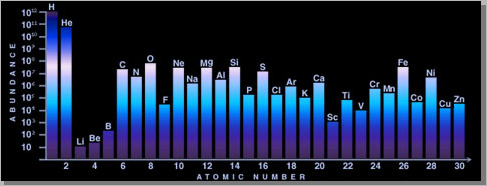
\includegraphics[scale=0.75]{Figures/atomic1.jpg} 
    \caption{Η αφθονία των χημικών στοιχείων στο σύμπαν.}  
    \label{fig:abundace_of_elements}
\end{figure}

Το αποτύπωμα της κοσμικής πυρηνοσύνθεσης βαρέων στοιχείων βρίσκεται και μέσα στην αφθονία των στοιχείων του ηλιακού συστήματος (σχήμα \ref{fig:solar_abundance_of_elements}). Η ηλιακή φωτόσφαιρα και οι μετεωρίτες αντικατοπτρίζουν την χημική υπογραφή του νέφους μέσα από το οποίο γεννήθηκε ο ήλιος. Αυτή η αφθονία όμως, φαίνεται να εκφράζει την γενικότερη συμπεριφορά της δημιουργίας των πυρήνων στο σύμπαν. Αξίζει να παρατηρήσουμε τις κορυφές στα στοιχεία με ατομικούς αριθμούς $A =$ 80, 130 και 195 --οι οποίοι αντιστοιχούν σε μαγικούς αριθμούς-- καθώς η σύνθεση αυτών των στοιχείων προέρχεται αποκλειστικά μέσω των διεργασιών που αναλύουμε στο παράρτημα \ref{apx:nucleosynthesis}.

\begin{figure}
    \centering
    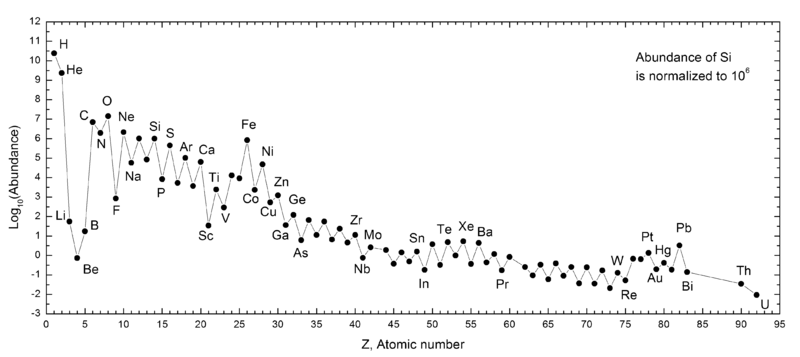
\includegraphics[scale=0.45]{Figures/SolarSystemAbundances.png} 
    \caption{Η αφθονία των χημικών στοιχείων στο ηλιακό μας σύστημα.}
    \label{fig:solar_abundance_of_elements}
\end{figure}

Σχεδόν όλη μάζα των στοιχείων συγκεντρώνεται στα στοιχεία του υδρογόνου και του ηλίου, τα οποία φαίνεται να παρήχθησαν κατά τη γέννηση του σύμπαντος. Η επικράτηση των πυρήνων μικρού ατομικού αριθμού $A$ έναντι των μεγαλυτέρων δεν είναι τυχαία και φαίνεται να οφείλεται σε δυο παράγοντες. Ο ένας παράγοντας είναι ότι σε μεγαλύτερους πυρήνες, η διαδικασία της σύντηξης απαιτεί μεγαλύτερη ενέργεια έτσι ώστε να ξεπεραστεί το απωστικό δυναμικό Coulomb καθώς η πιθανότητα μιας τέτοιας σύντηξης παρουσιάζει εκθετική εξάρτηση του προϊόντος από τα φορτισμένα αντιδρώντα. Για παράδειγμα, η σύντηξη δυο πυρήνων οξυγόνου θα  μας δώσει έναν πυρήνα 64 φορές μεγαλύτερο από εκείνον που θα μας δώσει η σύντηξη δυο πυρήνων υδρογόνου. Ο άλλος παράγοντας φαίνεται να είναι ο αριθμός των νουκλεονίων του πυρήνα. Όπως έχουμε δει και στα παραπάνω διαγράμματα, ο επόμενος εμφανιζόμενος πυρήνας με μονό αριθμό νουκλεονίων μετά το $^{1}$H είναι το $^{25}$Mg που είναι πολύ χαμηλός σε ποσοστά εμφάνισης. Με μια προσεκτικότερη ματιά στις χημικές αναλογίες είναι προφανές ότι υπάρχει μια προτίμηση στη δημιουργία πυρήνων με ζυγό αριθμό νουκλεονίων έναντι σε εκείνους με μονό αριθμό. Επίσης, φαίνεται να υπάρχει σαφής προτίμηση δημιουργίας πυρήνων που έχουν ζυγό-ζυγό αριθμό νουκλεονίων. Για παράδειγμα, στα πρώτα 25 στοιχεία μόνο το $^{14}$N δεν είναι ζυγός-ζυγός πυρήνας, δηλαδή δεν έχει ζυγό αριθμό πρωτονίων και ζυγό αριθμό νετρονίων. Επιπλέον εκτός από τον $^{56}$Fe όλοι οι υπόλοιποι συχνά εμφανιζόμενοι πυρήνες έχουν ζυγούς- ζυγούς πυρήνες αλλά και $Z=N$. Τους πυρήνες με αυτή την ιδιότητα τους ονομάζουμε \textbf{alpha-particle nuclei} εξαιτίας της ομοιότητάς του με τον πρώτο εμφανιζόμενο ζυγό-ζυγό πυρήνα, τον πυρήνα του $^{4}$He. Αυτό εξηγείται μέσω του πυρηνικού μοντέλου φλοιών, δηλαδή στο ότι οι ατομικοί πυρήνες αυξάνουν τις διαστάσεις τους σχηματίζοντας κελύφη γεμάτα με πρωτόνια και νετρόνια. Μόνο συγκεκριμένοι συνδυασμοί αριθμών πρωτονίων και νετρονίων φαίνεται να εμφανίζουν τους ισχυρότερους δεσμούς σύνδεσης και άρα ευσταθή στοιχεία. Τους συνδυασμούς αυτούς τους ονομάζουμε \textbf{μαγικούς αριθμούς}. Πλέον είναι προφανές ότι τα στοιχεία σε μεγαλύτερη αφθονία είναι εκείνα που έχουν διπλά μαγικούς όπως τα: $^{4}$He με $Z = N = 2$, $^{16}$O με $Z = N = 8$, $^{40}$Ca με $Z = N = 20$ και ακόμα και για τον σίδηρο $^{56}$Fe φαίνεται ότι αρχικά δημιουργήθηκε ως τον alpha-particle πυρήνα $^{56}$Ni με $Z = N = 28$. Μετά όμως από τη δημιουργία αυτού του στοιχείου, η διαδιακασία δημιουργίας βαρύτερων στοιχείων φαίνεται να αλλλάζει χαρακτήρα και να προέρχεται από μια διαφορετική διαδιακασία από εκείνη της σύντηξης. Την διαδικασία αυτή θα την αναλύσουμε εκτενώς παρακάτω και δεν είναι άλλη από εκείνη της αρπαγής νετρονίων. Τέλος, στο παρακάτω διάγραμμα Segre (σχήμα \ref{fig:segre_diagram}) φαίνεται μια ολοκληρωμένη εικόνα της τελικής εξέλιξης της πυρηνοσύνθεσης.

\begin{figure}
    \centering
    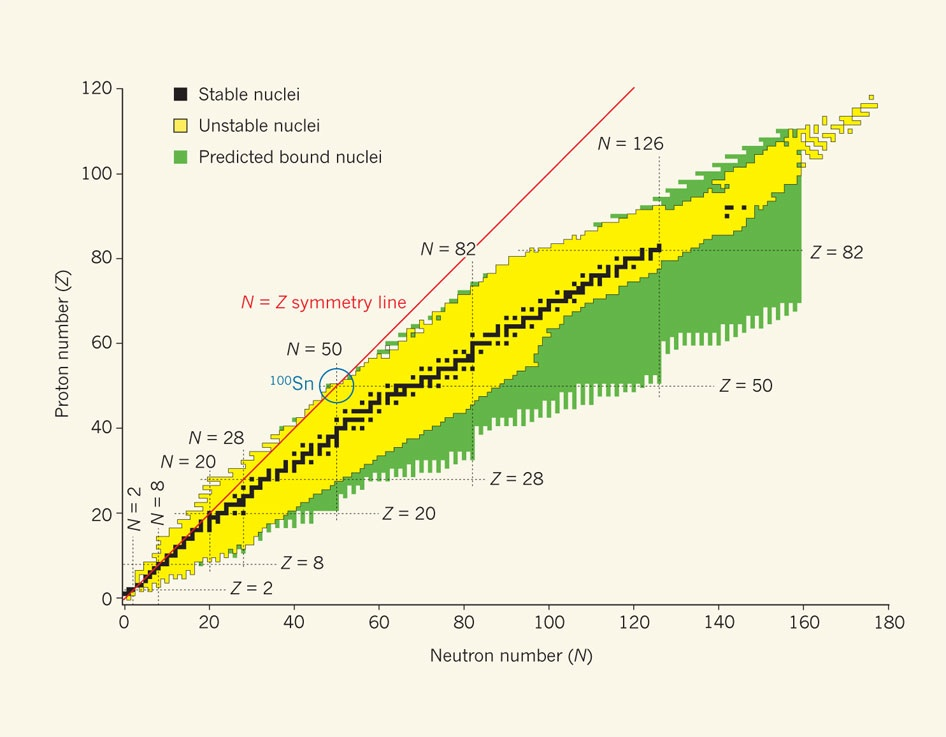
\includegraphics[scale=0.3]{Figures/Nuclei-as-function-of-N-Z.jpg} 
     \caption{Διάγραμμα Segre. Τα στοιχεία που εμφανίζονται με μαύρες κουκκίδες είναι σταθερά ισότοπα και αποτελούν την κοιλάδα σταθερότητας.} 
     \label{fig:segre_diagram}
\end{figure}
%% ---------------------------------------------------------------------------------------------------- %%
%% ---------------------------------------------------------------------------------------------------- %%
%% ---------------------------------------------------------------------------------------------------- %%
\subsection{Δημιουργία πρωτοαστέρων}
Τα άστρα δημιουργούνται κατά κανόνα από τη μεσοαστρική ύλη που υπάρχει στους γαλαξίες και η οποία αποτελείται κυρίως από υδρογόνο, ήλιο, και μοριακή σκόνη. Η ύλη αυτή, όπως και στο αρχέγονο σύμπαν, συχνά σχηματίζει νέφη τεραστίων διαστάσεων και χαμηλής πυκνότητας, τα νεφελώματα. Αυτά τα νέφη εξαιτίας της μεγάλης μάζας τους έχουν και την αντίστοιχη βαρυτική δυναμική ενέργεια, η οποία όμως λόγω της χαμηλής τους πυκνότητας, δεν είναι ικανή να υπερνικήσει τις θερμικές κινήσεις των μορίων και να προκαλέσει τη βαρυτική συστολή και συμπύκνωση.
Ο Jeans έδειξε ότι η δύναμη της πίεσης παύει να αντισταθμίζει τη βαρυτική έλξη, όταν οι διαστάσεις του νέφους είναι μεγαλύτερες, σε τάξη μεγέθους, από το \textbf{μήκος Jeans} που δίνεται απο τη σχέση
\begin{eqnarray}
    \label{eq:jeans_length}
    L_{\text{J}} = \left(\frac{14}{4\pi} \right)^{1/2} \left(\frac{kT}{\mu m_{\text{H}} G \rho} \right)^{1/2}
\end{eqnarray}
Στην περίπτωση αυτή όλη η ύλη, $M_{\text{J}}$, που περιέχεται σε μία σφαίρα με ακτίνα $L_{\text{J}}$, η οποία ισούται με
\begin{equation}
    \label{eq:jeans_mass}
    M_{\text{J}} = \frac{4}{3} \pi \rho L_{\text{J}} = \left(\frac{3}{4\pi \rho} \right)^{1/2} \left( \frac{5kT}{\mu m_{\text{H}} G} \right)^{3/2}
\end{equation}
συμπυκνώνεται και δημιουργεί ένα αστρικό αντικείμενο. Συμπερασματικά, η συμπύκνωση ευνοείται όταν η θερμοκρασία είναι μικρή, και η πυκνότητα μεγάλη. Ανάλογα με το μέγεθος της μάζας (το οποίο εξαρτάται από τη θερμοκρασία, την πυκνότητα και το μέσο μοριακό βάρος του αερίου), το αντικείμενο αυτό μπορεί να είναι ένας αστέρας, ένα σμήνος αστέρων ή και ένας γαλαξίας.

Για να εγκαταλείψει το νεφος την ισορροπία και να αρχίσει η συστολή απαιτείται μια αρχική διαταραχή, μήκους κύματος μεγαλύτερου ή ίσου με το χαρακτηριστικό μήκος Jeans γι' αυτό το νέφος. Διάφοροι παράγοντες μπορεί να επιφέρουν την βαρυτική κατάρρευση, μερικοί από τους οποίους είναι
  
  \begin{itemize}
  \item \textbf{Σύγκρουση Νεφών}\\
  Κατά τη σύγκρουση δυο ή περισσοτέρων νεφών η πυκνότητά τους αυξάνεται τοπικά δημιουργώντας έτσι περιοχές αστρογέννησης.
  
  \item \textbf{Έκρηξη Υπερκαινοφανούς Αστέρα (supernova)}\\
Όπως θα αναφέρουμε και παρακάτω, το τέλος ενός αστέρα μεγάλης μάζας συνοδεύται από την έκρηξή του. Σε μία τέτοια έκρηξη, το μεγαλύτερο μέρος ενός αστεριού (ή και ολόκληρο το αστέρι) διαλύεται και η ύλη του εκσφενδονίζεται βίαια στο διάστημα. Το ωστικό κύμα αυτής της έκρηξης συμπιέζει τα γειτονικά νέφη και δίνει το έναυσμα για τη βαρυτική συστολή.

  \item \textbf{Ύπαρξη νεαρών αστέρων μεγάλης μάζας}\\
 Όταν στην περιοχή των νεφών έχουν ήδη σχηματισθεί νέα μεγάλα αστέρια, αυτά εκπέμπουν τεράστια ποσά ακτινοβολίας η πίεση της οποίας επιδρά πάνω στην ύλη των γειτονικών νεφών και κάτω από τις κατάλληλες συνθήκες μπορεί να επιφέρει βαρυτική κατάρρευση.
 
 \item \textbf{Σπειροειδή Κύματα Πυκνότητας}\\
Σύμφωνα με τη θεωρία κυμάτων πυκνότητας (Lin και Shu, 1963), σπειροειδή κύματα πυκνότητας ξεκινούν από τον πυρήνα του γαλαξία και ξετυλίγονται προς τα έξω στον γαλαξιακό δίσκο. Τα κύματα αυτά συμπιέζουν το αέριο του δίσκου στα σημεία διεύλευσής τους προκαλώντας τη βαρυτική συστολή των μεσοαστρικών νεφών και τη δημιουργία νέων άστρων. Σε κάθε περίπτωση η παρουσία της πίεσης είναι απαραίτητη για να υπερνικηθούν οι τυχαίες θερμικές κινήσεις των μορίων.
\end{itemize}

Αυτή η βαρυτική κατάρρευση έχει ως επακόλουθο την εξώθερμη σύντηξη του υδρογόνου. Από τη στιγμή που σε ένα αστέρι ξεκινήσουν οι  θερμοπυρηνικές αντιδράσεις στον πυρήνα του, αρχίζει να ακτινοβολεί έντονα και ξεκινάει τη "ζωή" του. Αστέρια με μεγάλη μάζα έχουν μεγάλη βαρύτητα, συνεπώς μεγάλη πίεση και θερμοκρασία στον πυρήνα τους. Έτσι, οι συγκρούσεις μεταξύ των πυρήνων υδρογόνου είναι συχνότερες με αποτέλεσμα ο ρυθμός μεταστοιχείωσης του υδρογόνου να είναι μεγάλος. Επομένως, η παραγωγή και η ακτινοβολία ενέργειας είναι επίσης μεγάλες, έτσι ώστε τα αστέρια με μεγάλη μάζα να έχουν μεγάλη επιφανειακή θερμοκρασία και λαμπρότητα. Αντιθέτως, αστέρια με μικρή μάζα ακτινοβολούν λιγότερο. Οι μάζες των αστεριών ποικίλουν αλλά εντός συγκεκριμένων ορίων ($0.08 M_{\odot}<M<150 M_{\odot}$).
%% ---------------------------------------------------------------------------------------------------- %%
%% ---------------------------------------------------------------------------------------------------- %%
%% ---------------------------------------------------------------------------------------------------- %%
\subsubsection{Γραμμή Hayashi}
Η γενικά παραδεκτή σήμερα θεωρία εξέλιξης των πρωτοαστέρων είναι αυτή που πρότεινε ο Ιάπωνας αστρονόμος Hayashi. Στην αρχή το μεσοαστρικό νέφος που συστέλελται είναι οπτικά διαφανές (οπτικό βάθος $\tau \ll 1$) επειδή η πυκνότητά του είναι μικρή. Έτσι η ενέργεια που παράγεται στο εσωτερικό του, λόγω της βαρυτικής συστολής, ακτινοβολείται ελεύθερα στο μεσοαστρικό χώρο. Κατά τη διάρκεια αυτής της φάσης η θερμοκρασία στο εσωτερικό του νέφους παραμένει σταθερή και ίση με την αρχική, δηλαδή της τάκης των $10 \,\text{K}$. Γρήγορα, όμως, η πυκνότητα αυξάνει σημαντικά (καταρχήν στο κέντρο και αργότερα στις υπόλοιπες περιοχές), οπότε η ύλη παύει να είναι πια διαφανής. Στις περιοχές που η πυκνότητα ξεπερνά κάποια οριακή τιμή, η ύλη γίνεται αδιαφανής ($\tau \approx 1$) και η θερμοκρασία αυτών των περιοχών αρχίζει να αυξάνει, επειδή η παραγόμενη, λόγω συστολής, ενέργεια δεν μπορεί να ακτινοβοληθεί ελεύθερα στο μεσοαστρικό χώρο. Έτσι αυξάνει, καταρχήν, η θερμοκρασία της επιφάνειας του "πυρήνα" του νέφους, από όπου προέρχεται και η ακτινοβολία που εκπέμπει ο πρωτοαστέρας.

Σύμφωνα λοιπόν με τα παραπάνω, το αρχικό νέφος αρχίζει να εκπέμπει φως, ενώ έχει ακόμη μεγάλες διαστάσεις και είναι ακόμη ψυχρό. Επομένως βρίσκεται στην επάνω δεξιά γωνία του διαγράμματος H-R. Καθώς το νέφος συστέλλεται, η λαμπρότητά του ελλατώνεται (επειδή ελλατώνεται η ακτίνα του) η δε θερμοκρασία της ακτινοβολούσας επιφάνειας παραμένει περίπου σταθερή (αρχική καθοδική πορεία στο σχήμα \ref{fig:hayashi_tracks}). Καθώς όμως η βαρυτική κατάρρευση συνεχίζεται, κάποτε η θερμοκρασία της ακτινοβολούσας επιφάνειας αρχίζει να αυξάνει σημαντικά, οπότε μεγαλώνει και η φωτεινότητα του πρωτοαστέρα. Στο διάγραμμα H-R ο αστέρας ακολουθεί την ανοδική πορεία της καμπύλης στο σχήμα \ref{fig:hayashi_tracks}.
\begin{figure}[h!]
    \centering
    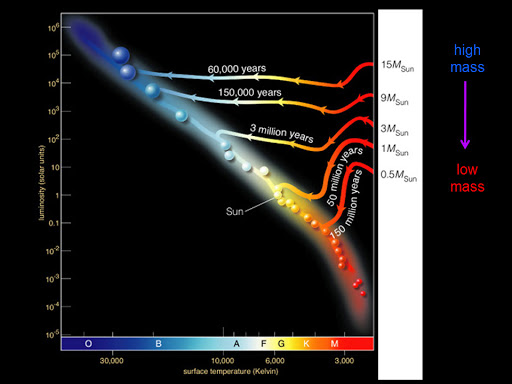
\includegraphics[scale=0.5]{Figures/hayashi_tracks.jpg}
    \caption{Πορείες Hayashi για πρωτοαστέρες διαφόρων μαζών και εγκατάστασή τους στην κύρια ακολουθία.}
    \label{fig:hayashi_tracks}
\end{figure}

Με την πάροδο του χρόνου αυξάνει και η πυκνότητα των εξωτερικών στρωμάτων, με αποτέλεσμα να γίνουν αδιαφανή σε οπτικά μήκη κύματος, ώστε η ακτινοβολία του πυρήνα να μην μπορεί να τα διαπεράσει πλέον. Επομένως, η ακτινοβολούσα επιφάνεια τείνει να συμπέσει με την τελική επιφάνεια του αστέρα. Από τη στιγμή αυτή και μετά, συμβαίνουν δύο βασικά γεγονότα:
\begin{enumerate}
    \item Η συστολή του πρωτοαστέρα συνεχίζεται, αν και με βραδύτερο ρυθμό, και επομένως η επιφάνειά του και η φωτεινότητά του ελλατώνονται (καθοδικό τμήμα της καμπύλης για πρωτοαστέρες με μικρή μάζα στο σχήμα \ref{fig:hayashi_tracks}.
    \item Η θερμοκρασία του πυρήνα αυξάνει σημαντικά, με αποτέλεσμα να αρχίσουν οι πρώτες θερμοπυρηνικές αντιδράσεις.
\end{enumerate}

Κατά τη διάρκεια της καύσης των διάφορων στοιχείων έχουμε ανάσχεση της βαρυτικής συστολής, επειδή η θερμική πίεση του αερίου αντισταθμίζει τη βαρυτική πίεση. Τα ελαφρά στοιχεία D, Li, Be, και B, τα οποία μεταστοιχειώνονται σε χαμηλές θερμοκρασίες, εξαντλούνται γρήγορα επειδή, όπως γνωρίζουμε από μετρήσεις της σχετικής αφθονίας των διάφορων στοιχείων στη φύση, είναι πολύ σπάνια. Όταν η θερμοκρασία φτάσει τους $\sim 10^7 \,\text{K}$, αρχίζει η καύση του άφθονου υδρογόνου σύμφωνα με τη σχέση \eqref{eq:4p_he4} και επιτυγχάνεται θερμική και υδροστατική ισορροπία. Ο αστέρας αρχίζει τη σταδιοδρομία του στην κύρια ακολουθία. Όσο πιο μεγάλη μάζα έχει ένας αστέρας όταν φτάσει στην κύρια ακολουθία, τόσο πιο θερμός και πιο φωτεινός είναι. Επομένως οι αστέρες μεγάλης μάζας εγκαθίστανται στο πάνω αριστερό τμήμα της κύριας ακολουθία, ενώ οι αστέρες μικρής μάζας στο κάτω δεξιό.

Η στιγμή της έναρξης της μεταστοιχείωσης του υδρογόνου στον πυρήνα ενός αστέρα, που συμπίπτει με την εγκατάστασή του στην κύρια ακολουθία, θεωρείται ως η αρχή της ζωής του, αντιστοιχεί δηλαδή σε μηδενική ηλικία. Η πορεία, στο διάγραμμα H-R, που ακολούθησε ο πρωτοαστέρας από τη στιγμή της δημιουργίας του μέχρι να φθάσει στη φάση ενός αστέρα μηδενικής ηλικίας ονομάζεται \textbf{πορεία Hayashi} (Hayashi track). Ο γεωμετρικός τόπος των θέσεων όλων των αστέρων μηδενικής ηλικίας στο διάγραμμα H-R ονομάζεται \textbf{κύρια ακολουθία μηδενικής ηλικίας} (zero age main sequence -- ZAMS). Το χρονικό διάστημα που μεσολαβεί από τη στιγμή της δημιουργίας του πρωτοαστέρα μέχρι τη στιγμή της εγκατάστασής του στην κύρια ακολουθία εξαρτάται από τη μάζα του: είναι μεγάλο για πρωτοαστέρες μικρής μάζας και μικρό για πρωτοαστέρες μεγάλης μάζας. Για τον Ήλιο αυτό το διάστημα υπολογίζεται ότι ήταν $\sim 2 \times 10^7 \,\text{yr}$. Από τα παραπάνω γίνεται σαφής και η διαφορά της ZAMS από την κύρια ακολουθία ενός σμήνους αστέρων: η ZAMS αποτελείται από τις θέσεις των αστέρων \textit{τη στιγμή της δημιουργίας τους}, ενώ η κύρια ακολουθία ενός συνόλου αστέρων (π.χ. ενός σμήνους) αποτελείται από θέσεις αστέρων \textit{διάφορων ηλικιών}, έστω και αν οι αστέρες αυτοί προέρχονται από πρωτοαστέρες που δημιουργήθηκαν ταυτόχρονα, αφού αστέρες διαφόρων μαζών χρειάζονται διαφορετικά χρονικά διαστήματα για να εγκατασταθούν στην κύρια ακολουθία. Επομένως, η ZAMS είναι ένα από πρότυπο χρήσιμο κυρίως για θεωρητικούς υπολογισμούς.
%% ---------------------------------------------------------------------------------------------------- %%
%% ---------------------------------------------------------------------------------------------------- %%
%% ---------------------------------------------------------------------------------------------------- %%
\subsection{Εξέλιξη μετά την κύρια ακολουθία}
Στο μεγαλύτερο μέρος της ζωής τους, οι αστέρες "καίνε" το υδρογόνο τους μετατρέποντάς το σε ήλιο σύμφωνα με τον κύκλο "πρωτονίου-πρωτονίου" (proton-proton chain) ή με τον κύκλο άνθρακα (κύκλος CNO). Όταν ένα σημαντικό ποσοστό του $^1$H μεταστοιχειωθεί σε $^4$He, ο ρυθμός των θερμοπυρηνικών αντιδράσεων ελαττώνεται και γίνεται μικρότερος από το ρυθμό ακτινοβολίας της επιφάνειας του άστρου. Έτσι, υπό την επίδραση της βαρύτητας και μέσω του μηχανισμού Kelvin-Helmholtz, η θερμοκρασία αυξάνεται και ξεκινά  η καύση του $^4$He προς $^{12}$C, με την προϋπόθεση η μάζα του αστέρα να είναι μεγαλύτερη των 0.4 ηλιακών μαζών.

 Η ενέργεια που παράγεται στον πυρήνα εξωθεί τα υπερκείμενα στρώματα με αποτέλεσμα την τεράστια διόγκωση του αστέρα και τη μετατροπή του σε ερυθρό γίγαντα. Αστέρες με μάζα ίση περίπου με την ηλιακή, κατά τη φάση του ερυθρού γίγαντα, χάνουν σε διάστημα 1000 ετών το 20\% με 30\% της μάζας τους σχηματίζοντας τελικά ένα \textit{πλανητικό νεφέλωμα}. Από την φάση του ερυθρού γίγαντα και μετά, ανάλογα με την μάζα ενός αστέρα διαφοροποιείται και η εξέλιξή του. 
%% ---------------------------------------------------------------------------------------------------- %%
%% ---------------------------------------------------------------------------------------------------- %%
%% ---------------------------------------------------------------------------------------------------- %%
\subsubsection{Αστέρες μικρής μάζας}
H συρρίκνωση του αδρανή (αστρικού) πυρήνα $^4$He συνεχίζεται με ταυτόχρονη παραγωγή ενέργειας, μέσω του μηχανισμού Kelvin-Helmholtz, μέχρι τη στιγμή που η αριθμητική πυκνότητα των ηλεκτρονίων σε αυτόν γίνει τόση ώστε αυτά να βρίσκονται σε κατάσταση εκφυλισμού. Για αστέρες με μάζα μικρότερη των $0.8 M_{\odot}$ αυτό συμβαίνει όσο η θερμοκρασία του πυρήνα είναι μικρότερη από τη θερμοκρασία "ανάφλεξης" του $^4$He. Ο αστρικός πυρήνας σταθεροποιείται σε αυτή την κατάσταση και μετατρέπεται σε έναν λευκό νάνο ηλίου. Τα υπόλοιπα στρώματα του αστέρα συνεχίζουν τη διαστολή τους με επιταχυνόμενο ρυθμό,  αντλώντας ενέργεια από την καύση του $^1$H στον φλοιό του αστέρα. Ταυτόχρονα όμως, η βαρυτική έλξη του πυρήνα γίνεται ασθενέστερη καθώς αυτά απομακρύνονται. Σε αυτό το σημείο, ο αστέρας περνά στην φάση του ερυθρού υπεργίγαντα. Κατά τη διάρκεια αυτού του σταδίου, ο αστέρας "σκορπίζεται" στην ευρύτερη περιοχή μέσω του έντονου αστρικού ανέμου που εμφανίζει, δημιουργώντας γύρω του ένα πλανητικό νεφέλωμα. To τελικό αποτέλεσμα είναι ένας λευκός νάνος θερμοκρασίας της τάξης των $30000 \,\text{K}$ που αποτελείται κυρίως από $^4$He και λίγο $^1$H.

%% ---------------------------------------------------------------------------------------------------- %%
%% ---------------------------------------------------------------------------------------------------- %%
%% ---------------------------------------------------------------------------------------------------- %%
\subsubsection{Αστέρες ενδιάμεσης μάζας}
Σε αυτή την κατηγορία έχουμε αστέρες με μάζα που βρίσκεται στο εύρος $0.8 \,M_{\odot} < M < 3 \,M_{\odot}$.
H εξέλιξη αυτών των αστέρων ακολουθεί την πορεία αυτών των μικρότερης μάζας εώς το στάδιο του ερυθρού γίγαντα. Σε αυτή την περίπτωση όμως, η δύναμη της βαρύτητας είναι σημαντικά ισχυρότερη με αποτέλεσμα τα ηλεκτρόνια του αδρανούς πυρήνα $^4$He να εκφυλίζονται και η θερμοκρασία του πυρήνα να ξεπερνά τη θερμοκρασία ανάφλεξης του $^4$He ($2\times 10^{8}K$). Τότε αρχίζει η καυση του $^4$He μέσω της διαδικασίας τριων-α που συζητήσαμε παραπάνω. Όταν όλο το $^4$He που βρίσκεται στον πυρήνα εξαντληθεί έχοντας μετατραπεί σε $^{12}$C και $^{16}$O, ξεκινά η καύση του $^4$He που εντοπίζεται στον εξωτερικό φλοιό του αστρικού πυρήνα, ενώ αυτός περιβάλλεται από έναν φλεγόμενο φλοιό $^1$H ακολουθώντας στο διάγραμμα H-R τον ασυμπτωτικό κλάδο των ερυθρών γιγάντων. Η τελική κατάσταση ενός τέτοιου αστέρα είναι η δημιουργία ενός λευκού νάνου άνθρακα-οξυγόνου.
%% ---------------------------------------------------------------------------------------------------- %%
%% ---------------------------------------------------------------------------------------------------- %%
%% ---------------------------------------------------------------------------------------------------- %%
\subsubsection{Αστέρες μεγάλης μάζας}
Η εξέλιξη αστέρων με μάζα μεγαλύτερη των $3M_{\odot}$ διαφέρει πλέον σημαντικά. Η χαρακτηριστικότερη διαφορά είναι ότι, μετά την εξάντληση των αποθεμάτων άνθρακα και οξυγόνου η θερμοκρασία του πυρήνα είναι πολύ υψηλή και ξεκινάει η μεταστοιχείωσή τους στο επόμενο βαρύτερο στοιχείο, το πυρίτιο (Si). Όσο μεγαλύτερη είναι η μάζα του πυρήνα, οι διαδοχικές μεταστοιχειώσεις προχωρούν μέχρι τη δημιουργία του σιδήρου (Fe). Σε αυτό το σημείο, η διαδικασία διακόπτεται καθώς η περαιτέρω μεταστοιχείωση του σιδήρου είναι μια ενδόθερμη αντίδραση και έτσι η αλυσίδα των συντήξεων σταματά. Σε αυτό το στάδιο, η δομή ενός αστέρα θυμίζει αυτή ενός κρεμμυδιού (onion-like structure) καθώς αποτελείται από πολλά διαφορετικά στρώματα-φλοιούς.
\begin{figure}[h!]
    \centering
    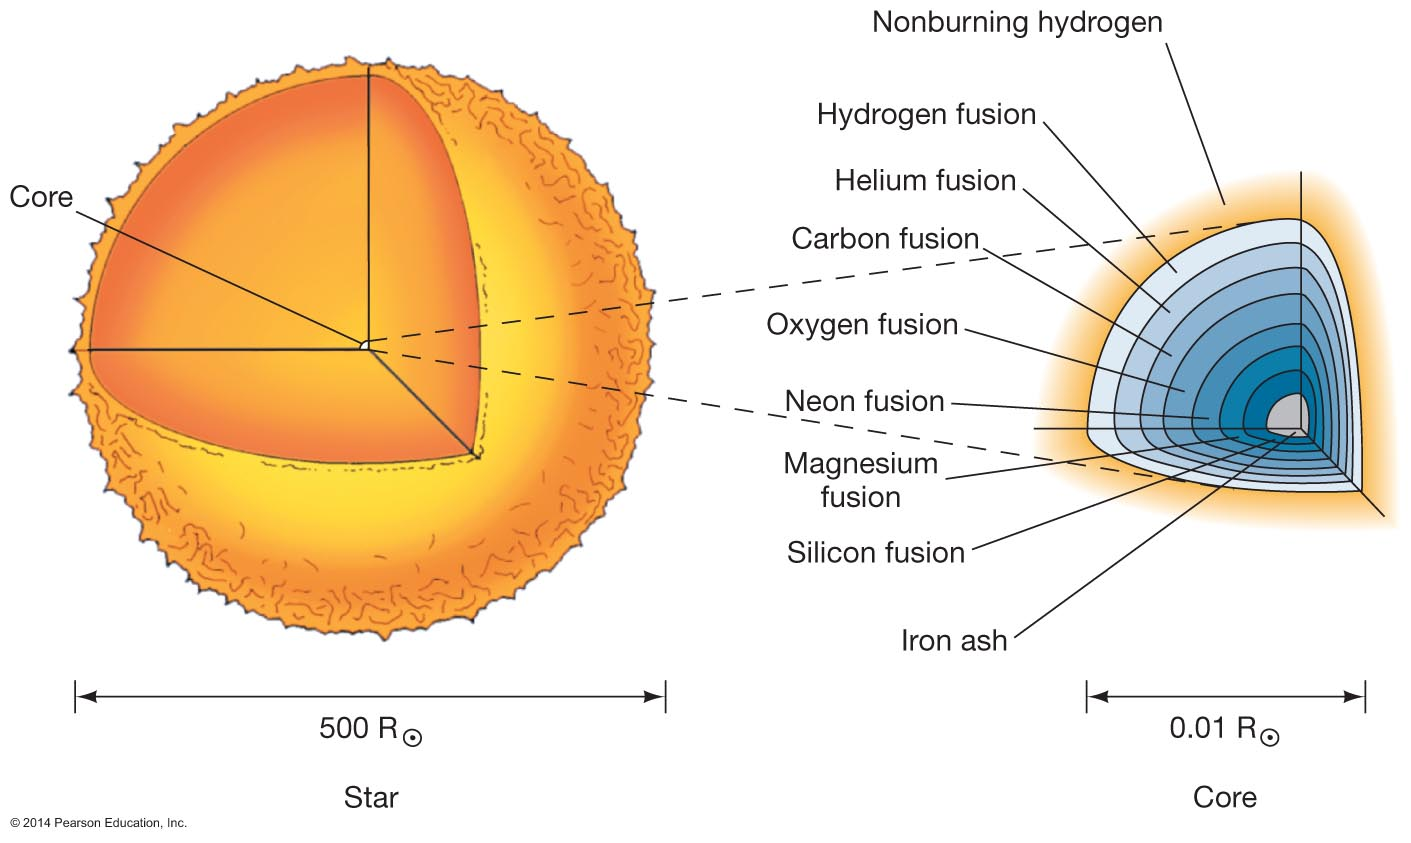
\includegraphics[scale=0.4]{Figures/onion_stellar_structure.jpg}
    \caption{Η δομή "κρεμμυδιού" και η καύση στοιχείων ανά φλοιό κατά τα τελευταία στάδια ζωής ενος αστέρα.}
    \label{fig:onion_stellar_structure}
\end{figure}

Η συνέχεια είναι σε κάθε περίπτωση --κυριολεκτικά-- καταστροφική για τον αστέρα. Με τις σημερινές γνώσεις που έχουμε στην αστροφυσική πιστεύουμε ότι μπορούν να υπάρξουν τέσσερις μόνο τελικές καταστάσεις στις οποίες είναι δυνατόν να καταλήξει ένας αστέρας όταν σταματήσει οριστικά η παραγωγή ενέργειας στον πυρήνα του: 

\begin{itemize}
\item Πλήρης διάλυση του αστέρα
\item Δημιουργία λευκού νάνου
\item Δημιουργία αστέρα νετρονίων
\item Δημιουργία μελανής οπής
\end{itemize}

 Η παραγωγή βαρύτερων στοιχείων του σιδήρου ξεκινά σε κάποιο από τα παραπάνω τελικά στάδια του αστέρα, με διάφορες διεργασίες που μπορούν να λάβουν χώρα και στις οποίες αναφερόμαστε εκτενώς στο παράρτημα \ref{apx:nucleosynthesis}.
%% ---------------------------------------------------------------------------------------------------- %%
%% ---------------------------------------------------------------------------------------------------- %%
%% ---------------------------------------------------------------------------------------------------- %%
\subsubsection{Εξέλιξη στο διάγραμμα H-R}
Η εξέλιξη αστέρων χαμηλής μάζας μπορεί να περιγραφεί ποιοτικά με τη βοήθεια του διαγράμματος H-R ενός σφαιρωτού σμήνους (σχήμα \ref{fig:hrd_evolution}. Παρόλο που το διάγραμμα H-R ενός σμήνους αποτελεί ένα στιγμιότυπο σε μία συγκεκριμένη χρονική στιγμή, παρουσιάζει όλα τα εξελικτικά στάδια στη ζωή ενός αστέρα καθώς η διάρκεια παραμονής ενός αστέρα σε κάθε εξελικτική φάση εξαρτάται από τη μάζα του.

\begin{figure}
    \centering
    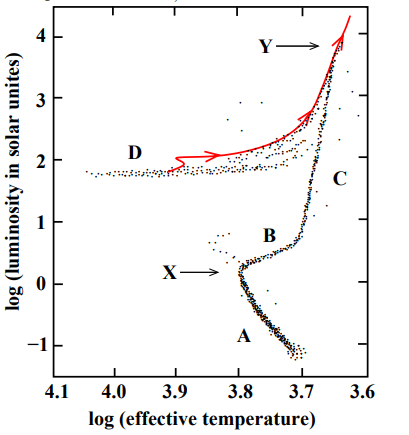
\includegraphics[scale=0.6]{Figures/hrd_evolution.png}
    \caption{Εξέλιξη αστέρων χαμηλής μάζας σε ένα σφαιρωτό σμήνος.}
    \label{fig:hrd_evolution}
\end{figure}

\begin{itemize}
    \item \textbf{Περιοχή A}: Παριστάνει την κύρια ακολουθία. Όλα τα αστέρια σε αυτή την περιοχή είναι στη φάση της κεντρικής καύσης του υδρογόνου, η οποία είναι και η μεγαλύτερη σε χρονική διάρκεια φάση στην ζωή του αστέρα. Αστέρες με χαμηλότερη λαμπρότητα κατά μήκος της κύριας ακολουθίας έχουν χαμηλότερη μάζα καθώς εγκαταστάθηκαν εκεί από διαφορετική πορεία Hayashi.
    \item \textbf{Σημείο στροφής X}: Αστέρες κοντά σε αυτό το σημείο έχουν (σχεδόν) εξαντλήσει το απόθεμα του υδρογόνου στον πυρήνα τους και είναι έτοιμα να αναπτύξουν, πρώτα έναν ισοθερμικό, και έπειτα έναν ηλεκτρονιακά εκφυλισμένο πυρήνα, αφήνωντας πίσω τους την κύρια ακολουθία με το να μετακινηθούν προς χαμηλότερες θερμοκρασίες (δηλαδή την περιοχή B). Παρατηρήστε ότι υπάρχουν μερικά άστρα στην προέκταση της κύριας ακολουθίας, μετά το σημείο στροφής X. Αυτοί οι αστέρες ονομάζονται "κυανοί περιπατητές" (blue stragglers) και είναι ελαφρώς πιο μεγάλοι (σε μάζα) αστέρες που δεν έχουν εξελιχθεί ακόμα πέρα από την κύρια ακολουθία. Αυτά τα αστέρια είναι πιθανόν το αποτέλεσμα των αλληλεπιδράσεων με κάποιο συνοδό αστέρα, ή δημιουργήθηκαν με τη σύγκρουση και συγχώνευση με κάποιο άλλο άστρο στο σφαιρωτό σμήνος (κάτι που συμβαίνει αρκετά συχνά στα πυκνά σφαιρωτά σμήνη).
    \item \textbf{Περιοχές B και C}: Με την έξοδό τους από την κύρια ακολουθία, οι αστέρες γίνονται μεγαλύτεροι (σε διαστάσεις) και πιο λαμπροί και μεταμορφώνονται σε υπογίγαντες (περιοχή B) και τελικά σε γίγαντες (περιοχή C). Στη φάση των γιγάντων, εξελίσσονται με σχεδόν σταθερή ενεργό θερμοκρασία $T_{\text{eff}}$. Σε αυτή τη φάση, οι αστέρες έχουν έναν εκφυλισμένο συμπαγή πυρήνα ο οποίος περιτριγυρίζεται από μία ατμόσφαιρα (convective envelope) που καταλαμβάνει τον μεγαλύτερο όγκο του αστέρα. Η καύση του υδρογόνου συνεχίζεται σε έναν φλοιό που περιβάλλει τον πυρήνα.  
    \item \textbf{Σημείο στροφής Y}: Σε αυτό το σημείο ξεκινάει η καύση του ηλίου στον πυρήνα του αστέρα. Επειδή ο πυρήνας αποτελείται από εκφυλισμένο αέριο ηλεκτρονίων, η ανάφλεξη του ηλίου είναι βίαιη και οδηγεί σε αναπροσαρμογή της δομής του αστέρα (έκλαμψη ηλίου -- helium flash). Παρόλα αυτά, η εκλαμψη δεν είναι αρκετά εκρηκτική για να διαλύσει τον αστέρα. Αντ' αυτού, ο αστέρας επαναπροσαρμόζει τη δομή του και καταλήγει στον οριζόντιο κλάδο του διαγράμματος (περιοχή D). Γι' αυτό, η έκλαμψη ηλίου σηματοδοτεί μία προσωρινή αύξηση στην λαμπρότητα του αστέρα, ορίζοντας την κορυφή του κλάδου των γιγάντων.
    \item \textbf{Περιοχή D}: Αφού επανέλθει σε κατάσταση υδροστατικής και θερμικής ισορροπίας, ο αστέρας περνάει σημαντικό μέρος της ζωής του στον οριζόντιο κλάδο, όπου καίει τα αποθέματα ηλίου στον πυρήνα του, ο οποίος είναι περιτριγυρισμένος από έναν φλοιό στον όποιο πραγματοποιείται καύση υδρογόνου (αυτή είναι συνήθως και η κύρια πηγή ενέργειας). Όταν εξαντληθούν τα αποθέματα του ηλίου στο κέντρο του αστέρα, επιστρέφει στη φάση του ερυθρού γίγαντα με την πορεία που ακολουθεί να προσεγγίζει ασυμπτωτικά τον αρχικό κλάδο των γιγάντων. Σε αυτή την ασυμπτωτική φάση (AGB phase), ο αστέρας έχει έναν εκφυλισμένο πυρήνα που αποτελείται από άνθρακα και οξυγόνο, και περιτριγυρίζεται από έναν φλοιό πλούσιο σε ήλιο και μία πλούσια σε υδρογόνο ατμόσφαιρα. Η πηγή ενέργειας είναι η θερμοπυρηνική σύντηξη του υδρογόνου και του ηλίου που συμβαίνουν σε λεπτούς σφαιρικούς φλοιούς γύρω από τον αδρανή εκφυλισμένο πυρήνα. 
    Επειδή σε αυτό το στάδιο, η ένταση του αστρικού ανέμου είναι πολύ μεγάλη, ο αστέρας χάνει τα εξωτερικά του στρώματα εκθέτοντας τους φλοιούς στους οποίους έχουμε ακόμα καύση. Ο αστέρας έχει πλέον περάσει στη φάση του πλανητικού νεφελώματος στο διάγραμμα H-R και αρζίσει να κινείται προς υψηλότερες θερμοκρασίες με περίπου σταθερή λαμπρότητα. Αυτό συμβαίνει επειδή αρχίζουμε και βλέπουμε πλέον τον πυρήνα του αστέρα που είναι θερμός ενώ η παραγωγή ενέργειας στους φλοιούς παραμένει η ίδια.
    Σε κάποια φάση, η πυρηνική καύση στους φλοιούς θα σταματήσει και ο αστέρας θα αποτινάξει τελείως την ατμόσφαιρά του εκθέτοντας τον πυρήνα του (λευκός νάνος), ο οποίος θα συνεχίσει να ψύχεται εως ότου φτάσει σε θερμική ισορροπία με το υπόλοιπο Σύμπαν.
\end{itemize}
%% ---------------------------------------------------------------------------------------------------- %%
%% ---------------------------------------------------------------------------------------------------- %%
%% ---------------------------------------------------------------------------------------------------- %%
%     \chapter{Δομή και εξέλιξη αστέρων}
\label{ch:Chapter5}
{\hypersetup{linkcolor=black, pdfborder=0 0 1}
	\minitoc
	%\newpage
}

Όλες οι παρατηρούμενες ιδιότητες που έχουμε αναφέρει μέχρι στιγμής, είναι ιδιότητες της επιφάνειας του αστέρα. Γι' αυτό χρειαζόμαστε μια θεωρία αστρικής δομής για να εξάγουμε συμπεράσματα για τις ``εσωτερικές'' ιδιότητες των άστρων. Παρόλα αυτά, υπάρχουν μερικά παράθυρα για την άμεση παρατήρηση του τι συμβαίνει στο εσωτερικό, όπως παρατηρήσεις νετρίνων (μέχρι στιγμής αυτό ισχύει μόνο για τον Ήλιο) και ταλαντώσεις που μας δίνουν πληροφορίες για την ταχύτητα που ταξιδεύουν τα ηχητικά κύματα στο εσωτερικό και άρα για την πυκνότητα και θερμοκρασία που επικρατούν.
%% ---------------------------------------------------------------------------------------------------- %%
%% ---------------------------------------------------------------------------------------------------- %%
%% ---------------------------------------------------------------------------------------------------- %%
\section{Εσωτερική δομή αστέρων}
Το πρότυπο αστρικής δομής που είναι σήμερα αποδεκτό προτείνει ότι η ενέργεια που ακτινοβολούν οι αστέρες εκλύεται στον πυρήνα τους από θερμοπυρηνικές αντδράσεις σύντηξης. Η ενέργεια αυτή διαδίδεται προς την επιφάνεια του αστέρα είτε με τη μορφή ακτινοβολίας είτε με ρεύματα μεταφοράς ύλης, και τελικα ακτινοβολείται από την επιφάνειά του προς το διάστημα. Για να γνωρίσουμε το εσωτερικό του Ήλιου (και άλλων αστέρων) βασιζόμαστε σε θεωρητικά επιχειρήματα, από τα οποία οδηγούμαστε τελικά σε ένα σύστημα διαφορικών εξισώσεων. Το σύστημα αυτό αποτελείται, στην απλούστερη μορφή του, από τέσσερις διαφορικές εξισώσεις και στη μορφή αυτή περιγράφει το θεωρητικό πρότυπο ενός σφαιρικά συμμετρικού, στατικού και μη-περιστρεφόμενου αστέρα, το υλικό του οποίου βρίσκεται σε υδροστατική και τοπική θερμοδυναμική ισορροπία.
%% ---------------------------------------------------------------------------------------------------- %%
%% ---------------------------------------------------------------------------------------------------- %%
%% ---------------------------------------------------------------------------------------------------- %%
\subsection{Μηχανική ισορροπία}
Η υπόθεση της σφαιρικής συμμετρίας έχει ως συνέπεια ότι όλες οι εξαρτημένες μεταβλητές του προβλήματος (πίεση $P$, πυκνότητα $\rho$, θερμοκρασία $T$ κτλ) είναι συνάρτηση μόνο της ακτινικής απόστασης, $r$, από το κέντρο του αστέρα, $r \in [0, \dots, R]$. Σε ένα αστέρι που εξελλίσεται όπως θα δούμε με τον χρόνο, όλες οι ποσότητες εξαρτώνται από τον χρόνο αλλά αυτό δεν θα είναι προφανές από τον τρόπο που θα παρουσιάσουμε τις εξισώσεις: μία παράγωγος $d/dr$ (ή $d/dm$) θα πρέπει να εκλαμβάνεται ως μερική παράγωγος ως προς τη χωρική συντεταγμένη υπό σταθερό χρόνο.
%% ---------------------------------------------------------------------------------------------------- %%
%% ---------------------------------------------------------------------------------------------------- %%
%% ---------------------------------------------------------------------------------------------------- %%
\subsubsection{Εξίσωση συνέχειας μάζας}
Έστω σφαιρικός φλοιός πάχους $dr$ σε απόσταση $r$ από το κέντρο του αστέρα (σχήμα \ref{fig:spherical_shell_hydrostatic_equilibrium}). Η αρχή της διατήρησης μάζας μας δίνει για τη στοιχειώδη μάζα, $dm$:
$$dm = \rho(r) dV$$
Ο όγκος του φλοιού θα είναι ουσιαστικά η επιφάνεια της εσωτερικής σφαίρας επί το στοιχειώδες πάχος. Αυτό αποδεικνύεται εύκολα ως εξής
$$dV = \frac{4}{3} \pi (r+dr)^3 - \frac{4}{3} \pi r^3 = \frac{4}{3} \pi \left[ (r+dr)^3 - r^3 \right] \simeq 4\pi r^2 dr$$ καθώς ο τετραγωνικός και κυβικός όρος του $dr$ στο ανάπτυγμα του πολυωνύμου μπορούν να θεωρηθούν ότι είναι περίπου μηδέν όταν $dr \ll r$. Αυτό μας οδηγεί στην πρώτη διαφορική εξίσωση που περιγράφει την δομή ενός αστέρα, την \textbf{εξίσωση συνέχειας μάζας}

\begin{equation}
    \label{eq:mass_continuity_diff}
    \boxed{\frac{dm}{dr} = 4 \pi r^2 \rho(r)} 
\end{equation}
Η εξίσωση αυτή περιγράφει το πως κατανέμεται η μάζα, και πως η κατανομή αυτή δεν έχει ασυνέχειες (δεν υπάρχουν τρύπες).


\begin{figure}
    \centering
    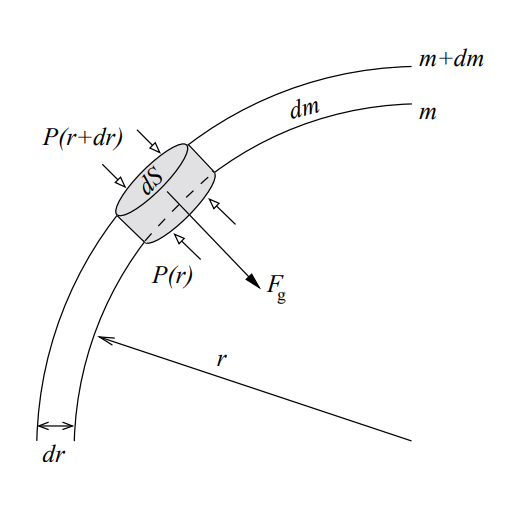
\includegraphics[scale=0.4]{Figures/spherical_shell_mechanical_equilibrium.png}
    \caption{Φλοιός σε ακτίνα $r$ και πάχος $dr$, μέσα σε σφαιρικά συμμετρικό αστέρι. Η μάζα του φλοιού είναι $dm = 4\pi r^2 \rho dr$. Στο σχήμα φαίνεται επίσης η πίεση και η βαρυτική δύναμη που ενεργούν σε ένα στοιχειώδες κυλινδρικό στοιχείο μάζας.}
    \label{fig:spherical_shell_hydrostatic_equilibrium}
\end{figure}

Η ολοκλήρωση της σχέσης \eqref{eq:mass_continuity_diff} μας δίνει την μάζα, $m(r)$, που περικλείει ένας σφαιρικός φλοιός ακτίνας $r$
\begin{equation}
        \label{eq:mass_coordinate}
    m(r) = \int_{0}^{R} 4\pi r^2 \rho(r) \,dr \hspace{0.5cm} (m \in 0,\dots,M)
\end{equation}

Επειδή η μάζα $m(r)$ αυξάνεται μονοτονικά προς την επιφάνεια του αστέρα, μπορούμε να χρησιμοποιήσουμε αυτή ως ακτινική συντεταγμένη αντί του $r$ (δηλαδή να χρησιμοποιήσουμε μια Λαγκραντζιανή περιγραφή αντί της μεθόδου του Euler). Έτσι η εξίσωση \eqref{eq:mass_coordinate} περιγράφει τη \textit{συντεταγμένη μάζας} (mass coordinate), η οποία είναι γενικευμένη συντεταγμένη (Lagrange coordinates) και κινείται μαζί με ένα στοιχειώδες κομμάτι του ρευστού. Αυτή η περιγραφή είναι προτιμότερη πολλές φορές καθώς η ακτίνα του αστέρα είναι συνάρτηση του χρόνου και μεταβάλλεται πολλές τάξεις μεγέθους κατά τη διάρκεια της εξέλιξής του.
Αντίθετα, η μάζα του μπορεί να θεωρηθεί σταθερή σε πρώτη φάση, γεγονός που απλοποιεί μερικές από τις χρονικές παραγώγους στις διαφορικές εξισώσεις που περιγράφουν την χημική σύσταση του αστέρα όπως θα δούμε. Έτσι, μπορούμε να γράψουμε όλες τις ποσότητες ως συνάρτηση της μάζας αντί του $r$ ως $r = r(m), \rho = \rho(m), P = P(m)$ κτλ. Κάνοντας τον μετασχηματισμό $r \rightarrow m$, η εξίσωση \eqref{eq:mass_continuity_diff} γράφεται ξανά:
\begin{equation}
    \label{eq:mass_continuity_diff_dm}
    \frac{d}{dm} = \frac{d}{dr} \cdot \frac{dr}{dm}  \longrightarrow \boxed{\frac{dr}{dm} = \frac{1}{4\pi r^2 \rho (r)}}
\end{equation}
%% ---------------------------------------------------------------------------------------------------- %%
%% ---------------------------------------------------------------------------------------------------- %%
%% ---------------------------------------------------------------------------------------------------- %%
\subsubsection{Το βαρυτικό πεδίο}
Τα αστέρια είναι αέρια σώματα που υποστηρίζονται από την ίδια τους την βαρύτητα (self-gravitating bodies), πράγμα που σημαίνει ότι η βαρύτητα παίζει καταλυτικό ρόλο στην εξέλιξή τους. Στη γενική, μη-σφαιρική περίπτωση, η βαρυτική επιτάχυνση είναι η κλίση (gradient) του βαρυτικού δυναμικού $\Phi$
$$\boldsymbol{g} = - \nabla \Phi$$
όπου το $\Phi$ είναι λύση της εξίσωσης Poisson 
\begin{equation}
    \label{eq:poisson_equation}
    \nabla^2 \Phi = 
    \begin{cases}
        0 & \text{για r > R}\\
        4\pi G \rho & \text{για r < R}
    \end{cases}
\end{equation}

Για μία σφαιρική κατανομή μάζας $M$, μπορούμε να θεωρήσουμε ότι όλη η μάζα είναι συγκεντρωμένη σε ένα σημείο στο κέντρο. Τότε, το βαρυτικό δυναμικό $\Phi$ σε απόσταση $r>R$ από το κέντρο, ισούται με το έργο ανά μονάδα μάζας που απαιτείται για να φέρουμε ένα σώμα μάζας $m$ από το άπειρο, σε αυτό το σημείο
\begin{equation}
    \Phi = \frac{1}{m}\int_{\infty}^{r} \boldsymbol{F_{\text{gr}}} \cdot d\boldsymbol{r} = \frac{1}{m} \int_{\infty}^{r} G\frac{M \,m }{r^2} \,dr \Rightarrow \Phi = - \frac{G \,M}{r}
\end{equation}
H βαρυτική επιτάχυνση γράφεται απλά $g = d\Phi / dr$ και σε ακτίνα $r$ (ή ισοδύναμα σε συντεταγμένη μάζας $m$) δίνεται από 
\begin{equation}
    \label{eq:gravitational_field}
    g = G \frac{m}{r^2}
\end{equation}
Σφαιρικοί φλοιοί που βρίσκονται σε ακτίνα μεγαλύτερη από $r$ δεν εφαρμόζουν κάποια δύναμη, άρα το $g$ εξαρτάται μόνο από την κατανομή της μάζας μέσα στον φλοιό ακτίνας $r$ (shell theorem). Το συμπέρασμα αυτό μπορεί να αποδειχθεί με τη βοήθεια του νόμου του Gauss από τον διανυσματικό λογισμό σύμφωνα με τον οποίο "το επιεπιφάνειο ολοκλήρωμα μια διανυσματικής συνάρτησης σε μια κλειστή επιφάνεια S ισούται με το τριπλό ολοκλήρωμα της απόκλισης (divergence) της διανυσματικής αυτής συνάρτησης στον όγκο V που περικλείεται από την κλειστή επιφάνεια"
\begin{equation}
    \label{eq:gauss_law_vector_calculus}
    \oiint_S \boldsymbol{f} \cdot d \boldsymbol{S} = \iiint_V (\nabla \cdot \boldsymbol{f}) \,dV 
\end{equation}
Θέτωντας $\boldsymbol{f} = \boldsymbol{g}$, προκύπτει ότι το αριστερό μέλος της σχέσης \eqref{eq:gauss_law_vector_calculus} γράφεται
\begin{equation}
    \label{eq:left_hand_side_gauss_law}
    \oiint_S \boldsymbol{g} \cdot d \boldsymbol{S} = \oiint_S (\boldsymbol{g} \cdot \hat{\eta}) \, dS = - 4\pi r^2 g
\end{equation}
Το παραπάνω αποτέλεσμα προκύπτει από τη σφαιρική συμμετρία του βαρυτικού πεδίου του αστέρα. Λόγω της συμμετρίας αυτής το πεδίο έχει μόνο ακτινική συνιστώσα, η οποία μάλιστα έχει σταθερή τιμή πάνω στη σφαιρική επιφάνεια S. Άρα, με την ένταση του βαρυτικού πεδίου να βγαίνει εκτός ολοκληρώματος, το κλειστό επικαμπύλιο ολοκλήρωμα ισούται με την επιφάνεια της σφαίρας με ακτίνα $r$. Το μείον προκύπτει επειδή το $\boldsymbol{g}$ με το διάνυσμα επιφάνειας $d\boldsymbol{S} = dS \cdot \hat{\eta}$ είναι συγγραμικά αλλά αντίρροπα.

Για το δεξιό μέλος της εξίσωσης \eqref{eq:gauss_law_vector_calculus}, πρέπει να βρούμε την απόκλιση της βαρυτικής επιτάχυνσης $(\nabla \boldsymbol{g})$. Από την εξίσωση Poisson (σχέση \eqref{eq:poisson_equation}), προκύπτει ότι
\begin{equation}
    \label{eq:right_hand_side_gauss_law}
    \nabla \boldsymbol{g} = \nabla (- \nabla \Phi) = - \nabla^2 \Phi = - 4\pi G \rho
\end{equation}
Συνδυάζοντας τις σχέσεις \eqref{eq:gauss_law_vector_calculus}, \eqref{eq:left_hand_side_gauss_law} και \eqref{eq:right_hand_side_gauss_law}, έχουμε ότι
\begin{equation}
    -4 \pi r^2 g = -4 \pi G \iiint_V \rho \,dV \Rightarrow g = G \frac{m(r)}{r^2}
\end{equation}
όπου το τριπλό ολοκλήρωμα μας δίνει απλά τη μάζα του αστέρα που περιέχεται μέσα σε μία σφαιρική επιφάνεια ακτίνας $r$ (σύμφωνα και με τη σχέση \eqref{eq:mass_coordinate}).
%% ---------------------------------------------------------------------------------------------------- %%
%% ---------------------------------------------------------------------------------------------------- %%
%% ---------------------------------------------------------------------------------------------------- %%
\subsubsection{Βαρυτική δυναμική ενέργεια}
Το να βρούμε τη συνολική βαρυτική δυναμική ενέργεια, $E_{\text{gr}}$, μιας μάζας όπως ο Ήλιος, φαίνεται εκ πρώτης όψεως μάταιο καθώς θα έπρεπε να αθροίσουμε τη δυναμική ενέργεια που προκαλεί κάθε ζεύγος σωματιδίων που αποτελούν τον Ήλιο. Το πρόβλημα απλουστεύται αν θεωρήσουμε ότι "κατασκευάζουμε" τον αστέρα με το να μεταφέρουμε στοιχειώδη σωματίδια από το άπειρο, ένα προς ένα (γι' αυτό και μερικές φορές αναφερόμαστε στην συνολική βαρυτική δυναμική ενέργεια ως ενέργεια σύνδεσης του αστέρα). Με αυτόν τον τρόπο, μεταφέρουμε ένα κομμάτι ύλης $dm$ στον μερικώς κατασκευασμένο αστέρα, που εκείνη τη στιγμή έχει μάζα $m$. Το κομμάτι αυτό της ύλης κατανείμεται συμμετρικά γύρω από τον αστέρα σχηματίζοντας έναν σφαιρικό φλοιό πάχους $dr$. Όπως είπαμε, η βαρυτική δύναμη που ασκείται σε ένα σωματίδιο έξω από μία σφαιρική κατανομή μάζας, όπως αυτή του Ήλιου, είναι ίδια σαν η μάζα να ήταν συγκεντρωμένη στο κέντρο του αστέρα. Γι' αυτό το λόγο, η δυναμική ενέργεια της μάζας $dm$ η οποία κατανέμεται συμμετρικά σε απόσταση $r$ από το κέντρο του αστέρα, είναι ίδια με τη δυναμική ενέργεια που θα είχαμε μεταξύ δύο σημειακών μαζών $dm$ και $m$ σε απόσταση $r$ μεταξύ τους. Έτσι, η διαφορά στη δυναμική βαρυτική ενέργεια του αστέρα θα ήταν
\begin{equation}
    dE_{\text{gr}} = E_{\text{gr}}^{dm}(r) - \cancelto{0}{E_{\text{gr}}^{dm}(\infty)} = - G \frac{m(r) \, dm}{r} 
\end{equation}
Ολοκληρώνοντας για όλες τις μάζες $dm$ μέσα στον φλοιό πάχους $dr$ σε απόσταση $r$ από το κέντρο έχουμε
\begin{equation}
    dE_{\text{gr}} = -G \int \frac{m(r) \,dm}{r} \xRightarrow{dm = \rho(r) \,dV} dE_{\text{gr}} = - G \frac{m(r) \,\rho(r) \, 4\pi r^2 \,dr}{r}
\end{equation}
όπου $dV = 4\pi r^2 \,dr$ ο όγκος του σφαιρικού φλοιού πάχους $dr$.

Ολοκληρώνοντας τώρα ως προς την ακτίνα του αστέρα, παίρνουμε την ολική βαρυτική δυναμική ενέργεια
\begin{equation}
    E_{\text{gr}} = -4\pi G \int_{0}^{R} m(r) \rho(r) \,r \,dr
\end{equation}
Γενικά, πρέπει να γνωρίζουμε το $\rho(r)$ για να βρούμε τη μάζα $m(r)$ η οποία είναι κι αυτή το ολοκλήρωμα
$$m(r) = \int_{0}^{m} dm = 4 \pi \int_{0}^{r} \rho(r) r^2 \,dr$$

Υποθέτωντας ότι 
\begin{equation}
    \rho(r) \approx \langle \rho \rangle = \frac{m}{\frac{4}{3} \pi R^3} \longrightarrow m(r) = \frac{4}{3} \pi r^3 \langle \rho \rangle
\end{equation}

Συνδυάζοντας όλα τα παραπάνω, προκύπτει τελικά ότι
\begin{align}
\label{eq:gravitational_potential_energy}
    \nonumber E_{\text{gr}} &= -4 \pi G \int_{0}^{R} \frac{4}{3} \pi r^3 \langle \rho \rangle^2 r \,dr \\\nonumber \\
    \nonumber &= -4\pi G \left( \frac{4\pi}{3} \right) \int_{0}^{R} r^4 \left( \frac{m}{\frac{4}{3} \pi R^3} \right)^2 \Rightarrow \\\nonumber \\
    &\Rightarrow \boxed{E_{\text{gr}} = - \frac{3Gm^2}{5R}}
\end{align}
%% ---------------------------------------------------------------------------------------------------- %%
%% ---------------------------------------------------------------------------------------------------- %%
%% ---------------------------------------------------------------------------------------------------- %%
\subsubsection{Υδροστατική ισορροπία}
Στη συνέχεια θα ασχοληθούμε με την αρχή διατήρησης της ορμής μέσα σε ένα αστέρι, δηλαδή με τον δεύτερο νόμο του Νεύτωνα. Η επιτάχυνση που δέχεται ένα στοιχειώδες κομμάτι αερίου καθορίζεται από το άθροισμα όλων των δυνάμεων που ενεργούν σε αυτό. Πέρα από την βαρυτική δύναμη, υπάρχουν και άλλες δυνάμεις που οφείλονται στην πίεση που ασκούν τα γειτονικά στρώματα αερίου πάνω στο υπο εξέταση στοιχειώδες κομμάτι. Λόγω της σφαιρικής συμμετρίας, οι δυνάμεις πίεσης που ασκούνται οριζόντια (κάθετα στην ακτινική διεύθυνση) εξισορροπούνται μεταξύ τους και άρα μόνο η δύναμη της πίεσης που ενεργεί κατά μήκος της ακτινικής διεύθυνσης πρέπει να ληφθεί υπόψιν. Άρα, η επιτάχυνση, $\boldsymbol{\ddot{r}}$, που δέχεται ένα στοιχειώδες κομμάτι αερίου μάζας
\begin{equation}
    \label{eq:dm}
    dm = \rho \,dr \,dS
\end{equation}
όπου $dr, dS$ είναι το στοιχειώδες πάχος και η στοιχειώδης οριζόντια επιφάνεια του κυλίνδρου (σχήμα \ref{fig:spherical_shell_hydrostatic_equilibrium}), θα είναι:
\begin{align}
    \label{eq:equation_of_motion_eulerian_coordinate}
    \nonumber dm \frac{\partial^2 \boldsymbol{r}}{\partial t^2} &\equiv \ddot{\boldsymbol{r}} \,dm = \boldsymbol{F}_{g} + \boldsymbol{F}_r + \boldsymbol{F}_{r+dr} = \\ \nonumber \\
    \nonumber & = -g \,dm + P(r) dS - P(r+dr) dS = \\ \nonumber \\
    \nonumber & = -g \,dm + dS \underbrace{\left[ P(r) - P(r+dr) \right]}_{-dP} = \\ \nonumber \\
    \nonumber & = -g \,dm - dP \,dS \Rightarrow \ddot{r} = -g - \frac{dP \,dS}{dm} \\ \nonumber \\
    &\xrightarrow[\text{\eqref{eq:gravitational_field}, \eqref{eq:dm}}]{\text{σχέσεις}} \ddot{r} = - G \frac{m}{r^2} - \frac{1}{\rho} \frac{dP}{dr}
\end{align}
Η σχέση \eqref{eq:equation_of_motion_eulerian_coordinate} είναι η \textit{εξίσωση κίνησης} για ένα στοιχειώδες κομμάτι αερίου μέσα στον αστέρα.

Xρησιμοποιώντας τη σχέση \eqref{eq:mass_continuity_diff_dm} στην βαθμίδα της πίεσης (pressure gradient), μπορούμε να γράψουμε ισοδύναμα την εξίσωση κίνησης εκφρασμένη σε συντεταγμένες μάζας ως
\begin{equation}
    \label{eq:equation_of_motion_lagrangian_coordinate}
    \ddot{r} = - G \frac{m}{r^2} - 4 \pi r^2 \frac{dP}{dm}
\end{equation}

Το γεγονός ότι η ακτίνα του Ήλιου παραμένει σταθερή εδώ και εκατομμύρια χρόνια, το γνωρίζουμε τόσο από ηλιακές όσο και γεωλογικές παρατηρήσεις. Εφόσον λοιπόν ο Ήλιος ούτε συστέλλεται ούτε διαστέλλεται, οι δυνάμεις που ασκούνται σε καθεμιά από τις δύο πλευρές κάθε επιφάνειας στο εσωτερικό του θα είναι ίσες και αντίθετες (σε αντίθετη περίπτωση η επιφάνεια αυτή δεν θα παρέμεινε ακίνητη). Με άλλα λόγια, η επιτάχυνση κατά την ακτινική διεύθυνση θα είναι μηδέν. Θέτωντας $\ddot{r} = 0$ στην εξίσωση κίνησης που δίνεται από τη σχέση \eqref{eq:equation_of_motion_eulerian_coordinate}, προκύπτει ότι
\begin{equation}
    \label{eq:hydrostatic_equilibrium_eulerian coordinates}
    \boxed{\frac{dP}{dr} = - G \frac{m(r) \rho(r)}{r^2}}
\end{equation}
ή, ισοδύναμα, σε συντεταγμένες μάζας
\begin{equation}
    \label{eq:hydrostatic_equilibrium_lagrangian_coordinate}
    \boxed{\frac{dP}{dm} = - G \frac{m(r)}{4\pi r^4}}
\end{equation}

Η εξίσωση \eqref{eq:hydrostatic_equilibrium_eulerian coordinates} αποτελεί τη δεύτερη διαφορική εξίσωση της αστρικής δομής, ονομάζεται εξίσωση \textit{υδροστατικής ισορροπίας}, και ισχύει όταν ο αστέρας βρίσκεται σε μηχανική ισορροπία (όταν δηλαδή οι δυνάμεις που ασκούνται σε ένα στοιχειώδες κομμάτι αερίου, εξισορροπούνται μεταξύ τους). Μαζί με την εξίσωση συνέχειας της μάζας (σχέση \eqref{eq:mass_continuity_diff}), προσδιορίζουν την \textit{μηχανική δομή} (mechanical structure) ενός αστέρα.

Άμεση συνέπεια της εξίσωσης \eqref{eq:hydrostatic_equilibrium_eulerian coordinates}, είναι ότι η πίεση σε έναν αστέρα που βρίσκεται σε υδροστατική ισορροπία \textit{πρέπει} να αυξάνεται όσο πλησιάζουμε το κέντρο του, ώστε να μπορεί να υποστηρίξει το βάρος των υπερκείμενων στρωμάτων.\\

{\color{red} \hrule}
\underline{Παρατήρηση}: Ένα αντικείμενο για να βρίσκεται σε κατάσταση υδροστατικής ισορροπίας, πρέπει να έχει αρκετή μάζα ώστε η βαρυτική δύναμη να είναι υπολογίσιμη. Έτσι, σώματα όπως η Σελήνη ή η Γη βρίσκονται σε κατάσταση υδροστατικής ισορροπίας, αλλά αντικείμενα όπως οι αστερεοιδείς όχι. Τα αντικείμενα αυτά υποστηρίζονται από τη φυσική ακαμψία τους (rigidity) η οποία οφείλεται στις ηλεκτρομαγνητικές αλληλεπιδράσεις των μορίων που τα αποτελούν.\\
{\color{red} \hrule}

Αξίζει να σημειωθεί ότι για να καταλήξουμε στην εξίσωση \eqref{eq:hydrostatic_equilibrium_eulerian coordinates} δεν κάναμε καμία υπόθεση για τη φύση της πίεσης που υπεισέρχεται στην εξίσωση αυτή, δηλαδή για τους μικροφυσικούς μηχαισμούς που παρουσιάζονται μακροσκοπικά ως πίεση. Από τη βασική Φυσική είναι γνωστοί ήδη δύο τέτοιοι μηχανισμοί, που μακροσκοπικά χαρακτηρίζονται ως \textit{πίεση αερίου}, $P_{\text{gas}}$, και \textit{πίεση ακτινοβολίας}, $P_{\text{rad}}$. Στη συνέχεια θα συναντήσουμε και έναν τρίτο μηχανισμό, που χαρακτηρίζεται μακροσκοπικά ως \textit{πίεση εκφυλισμένης ύλης}, $P_{\text{deg}}$. Στη γενικότερη περίπτωση λοιπόν θα πρέπει να χρησιμοποιούμε την ολική πίεση
$$ P = P_{\text{gas}} + P_{\text{rad}} + P_{\text{deg}}$$
όπου η πίεση του αερίου δίνεται από τον νόμο των τέλειων αερίων (σχέση \eqref{eq:ideal_gas_eos}), και η πίεση της ακτινοβολίας, $P_{\text{rad}}$, από τη σχέση \eqref{eq:radiation_pressure_black_body}. Ευτυχώς στο μεγαλύτερο ποσοστό των αστέρων, μεταξύ των οποίων συμπεριλαμβάνεται και ο Ήλιος, η πίεση της ακτινοβολίας και η πίεση της εκφυλισμένης ύλης είναι αμελητέες συγκρινόμενες με την πίεση του αερίου, και μπορούμε άνετα να τις παραλέιψουμε. Οι πιέσεις $P_{\text{rad}}$ και $P_{\text{deg}}$ γίνονται σημαντικές στις περιπτώσεις των πολύ μεγάλων, σε μάζα, αστέρων (η πρώτη) και των πολύ μικρών, σε διαστάσεις, αστέρων (η δεύτερη). Η ολοένα και αυξανόμενη πίεση της ακτινοβολίας όσο αυξανεται η μάζα των αστέρων είναι αυτή που θέτει και ένα ανώτερο όριο στη μάζα που μπορεί να έχει ένας αστέρας. Από κάποια οριακή τιμής της μάζας και πάνω, η πίεση της ακτινοβολίας είναι τόσο μεγάλη που καταστρέφει το αστέρι.
%% ---------------------------------------------------------------------------------------------------- %%
%% ---------------------------------------------------------------------------------------------------- %%
%% ---------------------------------------------------------------------------------------------------- %%
\subsubsection{Καταστατικές εξισώσεις}
Οι εξισώσεις \eqref{eq:mass_continuity_diff_dm} και \eqref{eq:hydrostatic_equilibrium_lagrangian_coordinate}
αποτελούν ένα σύστημα δύο εξισώσεων με τρεις αγνώστες συναρτήσεις του $m$ ($r$, $P$ και $\rho$), οπότε δεν μπορούν να λυθούν χωρίς μία τρίτη συνθήκη. Αυτή η συνθήκη είναι συνήθως μία σχέση μεταξύ της πίεσης, $P$, και της πυκνότητας μάζας, $\rho$, την οποία ονομάζουμε \textit{καταστατική εξίσωση} (equation of state). Γενικά, η καταστατική εξίσωση εξαρτάται και από τη θερμοκρασία, $T$, οπότε η μηχανική δομή ενός αστέρα εξαρτάται επίσης και από την κατανομή της θερμοκρασίας στο εσωτερικό του, δηλαδή από τη θερμική δομή του. Σε κάποιες ειδικές περιπτώσεις, η καταστατική εξίσωση είναι ανεξάρτητη της $T$, και μπορεί να γραφτεί ως $P = P(\rho)$. Σε αυτές τις περιπτώσεις (γνωστές ως βαρυτροπικές ή πολυτροπικές), η μηχανική δομή ενός αστέρα γίνεται ανεξάρτητη από τη θερμική δομή του. Μία τέτοια περίπτωση είναι αυτή των λευκών νάνων όπως θα δούμε στη συνέχεια.

Γίνεται αντιληπτό πως η καταστατική εξίσωση περιγράφει τις μικροσκοπικές ιδιότητες της αστρικής ύλης, για μία δεδομένη πυκνότητα μάζας $\rho$, θερμοκρασία $T$, και χημικής σύστασης $X_i$. Συνήθως εκφράζεται ως σχέση μεταξύ της πίεσης και αυτών των ποσοτήτων:
\begin{equation}
    P = P(\rho, T, X_i)
\end{equation}

Αν θεωρήσουμε αρχικά για λόγους απλότητας πως ένας αστέρας αποτελείται εξ' ολοκλήρου από Υδρογόνο και συμπεριφέρεται ως ιδανικό αέριο, τότε η καταστατική εξίσωση θα δίνεται από την γνωστή καταστατική εξίσωση των τέλειων αερίων 
\begin{equation}
    P(r) = n(r) kT = \frac{\rho}{m_\text{H}} kT
\end{equation}
Θεωρώντας τώρα ότι ένας αστέρας αποτελείται από διάφορα χημικά στοιχεία, η μάζα μπορεί να αντικατασταθεί από τη μέση μάζα του αέριου μείγματος, $\overline{m}$, ώστε
\begin{equation}
    P = \frac{\rho}{\overline{m}} kT
\end{equation}

Ορίζοντας την ποσότητα του \textit{μέσου μοριακού βάρους}
\begin{equation}
    \mu \equiv \frac{\overline{m}}{m_{\text{H}}}
\end{equation}
η καταστατική εξίσωση για ένα μείγμα ιδανικού αερίου θα είναι
\begin{equation}
    \label{eq:ideal_gas_eos}
    \boxed{P = \frac{\rho}{\mu m_{\text{H}}} k T }
\end{equation}
Προφανώς ο βαθμός ιονισμού του αερίου, κβαντομηχανικά (εκφυλισμός) και σχετικιστικά φαινόμενα επηρεάζουν την μορφή της καταστατικής εξίσωσης που πρέπει να λάβουμε υπόψιν κάθε φορά που θέλουμε να μελετήσουμε τη δομή ενός αστέρα. 

Η πίεση σχετίζεται και με την εσωτερική ενέργεια ενός αερίου. Για καταστατικές εξισώσεις αερίων που δεν είναι ιδανικά, υπάρχει μία σχέση μεταξύ της πίεσης και της εσωτερικής ενέργειας, την οποία μπορούμε να γράψουμε γενικά
\begin{equation}
    \label{eq:generic_eos}
    E_{\text{int}} = \phi \frac{P}{\rho} 
\end{equation}
Για το ιδανικό αέριο, η μέση εσωτερική ενέργεια ισούται με τη μέση κινητική ενέργεια (λόγω της θερμικής κίνησης των σωματιδίων) καθώς σε ένα μονοατομικό ιδανικό αέριο, τα σωματίδια δεν δονούνται και δεν περιστέφονται. Έτσι, μόνο η συνεισφορά της θερμικής (κινητικής) ενέργειας λαμβάνεται υπόψιν ώστε
\begin{equation}
    \label{eq:internal_energy_ideal_gas}
    \frac{\langle  E_{\text{int}} \rangle}{N} = \frac{\langle  E_{\text{kin}} \rangle}{N} = \frac{3}{2}kT
\end{equation}
όπου $N=\overline{m}/(\mu m_{\text{H}})$ είναι ο αριθμός των σωματιδίων. Oπότε για την περίπτωση του ιδανικού αερίου, $\phi = 3/2$. Αποδεικνύεται ότι αυτό ισχύει όχι μόνο στην περίπτωση του ιδανικού αερίου, αλλά για όλα τα μη-σχετικιστικά σωματίδια. Αντίθετα, αν θεωρήσουμε ένα αέριο που αποτελείται από σχετικιστικά σωματίδια, κυρίως φωτόνια (πίεση ακτινοβολίας), τότε προκύπτει ότι $\phi = 3$.

Με την καταστατική εξίσωση βρήκαμε μία σχέση μεταξύ της πίεσης και της πυκνότητας μάζας, αλλά εμφανίστηκε η άγνωστη παράμετρος της θερμοκρασίας. Το ότι η θερμοκρασία δεν είναι σταθερή σε όλη τη μάζα του αστέρα το γνωρίζουμε από διάφορα παρατηρησιακά δεδομένα όπως έχουμε πει, π.χ. αμαύρωση του χείλους, γραμμές απορρόφησης, και ότι το συνεχές φάσμα δεν ταυτίζεται με αυτό του μέλανος σώματος. Χρειαζόμαστε άρα και μία εξίσωση για το πως αλλάζει η θερμοκρασία προκειμένου να κλείσει το σύστημα των εξισώσεων.
%% ---------------------------------------------------------------------------------------------------- %%
%% ---------------------------------------------------------------------------------------------------- %%
%% ---------------------------------------------------------------------------------------------------- %%
\subsubsection{Θεώρημα virial}
Μία από τις συνέπεις της υδροστατικής ισορροπίας, είναι το θεώρημα virial. Το θεώρημα αυτό είναι παίζει καθοριστικό ρόλο σε διάφορα πεδία της Αστροφυσικής καθώς συνδέει δύο διαθέσιμες "δεξαμενές" ενέργειας επιτρέποντάς μας να ερμηνεύσουμε και να κάνουμε προβλέψεις για διάφορες φάσεις της αστρικής εξέλιξης.

Για να καταλήξουμε στο θεώρημα virial ξεκινάμε από την εξίσωση υδροστατικής ισορροπίας, \eqref{eq:hydrostatic_equilibrium_lagrangian_coordinate}. Πολλαπλασιάζοντας τα δύο μέλη με τον εσώκλειστο όγκο $V = \frac{4}{3}\pi r^3$ και ολοκληρώνοντας ως προς τη μάζα έχουμε
\begin{align*}
    \int_{0}^{M} \frac{4}{3} \pi r^3 \frac{dP}{dm} \,dm  = - \frac{1}{3} \underbrace{\int_{0}^{M} \frac{G \,m}{r} \,dm}_{= - E_{\text{gr}}} \Rightarrow \int_{\text{C}}^{\text{S}} V \,dP = \frac{1}{3} E_{\text{gr}}
\end{align*}
όπου οι τιμές S, C δηλώνουν επιφανειακές και κεντρικές τιμές αντίστοιχα. Το ολοκλήρωμα στο αριστερό μέλος μπορεί να λυθεί κατά παράγοντες ώστε
\begin{align}
    \label{eq:generic_form_virial}
    \nonumber &\left. V \,P \right|_{\text{C}}^{\text{S}} - \int_{\text{C}}^{\text{S}} P \,dV = \frac{1}{3} E_{\text{gr}} \Rightarrow V_{\text{S}}  \,\cancelto{0}{P_{\text{S}}} - \cancelto{0}{V_{\text{C}}} \,P_{\text{C}} - \\ \nonumber \\
    &- \int_{\text{C}}^{\text{S}} P \,dV = \frac{1}{3} E_{\text{gr}} \xRightarrow{dV = \rho \,dm} \boxed{E_{\text{gr}} = -3 \int_{0}^{M} \frac{P}{\rho} \,dm}
\end{align}

Η σχέση \eqref{eq:generic_form_virial} αποτελεί τη γενική μορφή του θεωρήματος virial και μας δείχνει ότι η μέση πίεση που χρειάζεται για να υποστηριχτεί ένας αστέρας σε υδροστατική ισορροπία είναι ίση με το $- \frac{1}{3} \frac{E_{\text{gr}}}{V}$. Συγκεκριμένα, μας δείχνει ότι ένας αστέρας ο οποίος συστέλλεται σχεδόν στατικά (δηλαδή αρκετά αργά ώστε να παραμένει σε υδροστατική ισορροπία) πρέπει να αυξάνει την εσωτερική του πίεση, αφού η βαρυτική δυναμική ενέργεια, $E_{\text{gr}}$, μειώνεται όσο μικραίνει η ακτίνα του αστέρα και γίνεται πιο συμπαγές (more tightly bound).


Όπως έχουμε πει, η πίεση σχετίζεται με την εσωτερική ενέργεια ενός αερίου. Στην περίπτωση που το αέριο αυτό είναι ιδανικό, τότε από τις σχέσεις \eqref{eq:ideal_gas_eos}, \eqref{eq:internal_energy_ideal_gas} και \eqref{eq:generic_form_virial}, προκύπτει ότι 
\begin{align*}
    \langle E_{\text{int}} \rangle = \langle E_{\text{kin}} \rangle = \frac{3}{2} \frac{P}{\rho} \mu m_{\text{H}} \longrightarrow u = \frac{\langle E_{\text{int}} \rangle}{\mu m_{\text{H}}}
\end{align*}
όπου με $u$ συμβολίζουμε την εσωτερική ενέργεια ανά μονάδα μάζας, και άρα η μορφή του θεωρήματος virial είναι
\begin{equation}
    \label{eq:ideal_gas_virial}
    E_{\text{gr}} = -3 \int_{0}^{M} \frac{P}{\rho} \,dm = - 2 \underbrace{\int_{0}^{M} u \,dm}_{E_{\text{int}}} \rightarrow \boxed{E_{\text{int}} = - \frac{1}{2} E_{\text{gr}}}
\end{equation}
 
Η σχέση \eqref{eq:ideal_gas_virial} θεμελιώνει ένα σύνδεσμο μεταξύ της βαρυτικής δυναμικής ενέργειας και της εσωτερικής (θερμικής) ενέργειας ενός αστέρα σε υδροστατική ισορροπία, ο οποίος αποτελείται από ιδανικό αέριο. Το θεώρημα virial μας λέει ότι όσο πιο συμπαγής γίνεται ένας αστέρας θα πρέπει να έχει και μεγαλύτερη εσωτερική ενέργεια, δηλαδή να είναι πιο θερμός. Με άλλα λόγια, ένας αστέρας που συστέλλεται σχεδόν στατικά πρέπει να γίνεται ολοένα και θερμότερος κατά τη διάρκεια της διαδικασίας. Το τι συνεπάγεται αυτό θα φανεί σε λίγο όταν αναλογιστούμε την ολική ενέργεια του αστέρα.

Στην περίπτωση που το αέριο δεν μπορεί να θεωρηθεί ιδανικό, δείξαμε ότι η σχέση μεταξύ της πίεσης και της εσωτερικής ενέργειας θα δίνεται από μία σχέση της μορφής της \eqref{eq:generic_eos}. Για $\phi = 3/2$ το αέριο είναι ιδανικό, ενώ για $\phi = 3$ το αέριο αποτελείται από σχετικιστικά σωματίδια. Αν το $\phi$ είναι σταθερό, τότε ολοκληρώνοντας τη σχέση \eqref{eq:generic_form_virial}, καταλήγουμε σε μια ακόμα πιο γενική μορφή του θεωρήματος virial
\begin{equation}
    \label{eq:generic_eos_virial}
    E_{\text{gr}} = - \frac{3}{\phi} \int_{0}^{M} \langle E_{\text{int}} \rangle \,dm \Rightarrow \boxed{ E_{\text{int}} = - \frac{1}{3} \phi  E_{\text{gr}}}
\end{equation}
%% ---------------------------------------------------------------------------------------------------- %%
%% ---------------------------------------------------------------------------------------------------- %%
%% ---------------------------------------------------------------------------------------------------- %%
\subsubsection{Ολική ενέργεια αστέρων}
Η ολική ενέργεια ενός αστέρα είναι το άθροισμα της βαρυτικής δυναμικής ενέργειας, της εσωτερικής του ενέργειας, και της κινητικής ενέργειας (λόγω της μαζικής κίνησης --bulk motion-- του αερίου μέσα στον αστέρα και όχι λόγω της θερμικής κίνησης των σωματιδίων του αερίου).
\begin{equation}
    \label{eq:total_energy_of_star_generic}
    E_{\text{tot}} =  E_{\text{gr}} +  E_{\text{int}} +  E_{\text{kin}}
\end{equation}
Ένας αστέρας εξακολουθεί να είναι δέσμιος (bound) όσο η ολική του ενέργεια είναι \textbf{αρνητική}.

Για έναν αστέρα σε υδροστατική ισορροπία μπορούμε να θέσουμε $ E_{\text{kin}} = 0$. Επίσης, για τον αστέρα που βρίσκεται σε υδροστατική ισορροπία ισχύει το θεώρημα virial, οπότε η $E_{\text{gr}}$ και η $E_{\text{int}}$ είναι στενά συνδεδμένες μέσω της σχέσης \eqref{eq:generic_eos_virial}. Συνδυάζοντας τις σχέσεις \eqref{eq:generic_eos_virial} και \eqref{eq:total_energy_of_star_generic} προκύπτουν οι ακόλουθες σχέσεις
\begin{equation}
    \label{eq:total_energy_of_star_with_generic_eos}
    E_{\text{tot}} = E_{\text{gr}} + E_{\text{int}} = \left( \frac{\phi - 3}{\phi} \right) E_{\text{int}} = \left( 1 - \frac{\phi}{3} \right) E_{\text{gr}}
\end{equation}
Παρατηρούμε ότι όσο το $\phi < 3$, ο αστέρας είναι δέσμιος. Αν θέσουμε $\phi = 3/2$, παίρνουμε την περίπτωση του ιδανικού αερίου οπότε η σχέση \eqref{eq:total_energy_of_star_with_generic_eos} γράφεται
\begin{equation}
    \label{eq:total_energy_of_star_ideal_gas}
     \boxed{E_{\text{tot}} = -  E_{\text{int}} = \frac{1}{2}  E_{\text{gr}} < 0}
\end{equation}
δηλαδή βλέπουμε πως για έναν τέτοιον αστέρα, η ολική του ενέργεια ισούται με το μισό της βαρυτικής δυναμικής του ενέργειας. 

Αν η κυρίαρχη πίεση στο εσωτερικό ενός αστέρα είναι η πίεση της ακτινοβολίας ($\phi = 3$), τότε βλέπουμε ότι η ολική του ενέργεια ισούται με μηδέν, καθώς $ E_{\text{int}} = -  E_{\text{gr}}$. Για αυτό το λόγο, αστέρες που υποστηριζόνται από την πίεση σχετικιστικών σωματιδίων είναι οριακά δέσμιοι, και συνεπώς εξαιρετικά ευαίσθητοι σε διαταραχές που μπορούν να οδηγήσουν στην κατάρρευση ή την έκρηξη του αστέρα. 


Από την σχέση \eqref{eq:total_energy_of_star_ideal_gas} προκύπτει ότι το θεώρημα virial έχει τις εξής συνέπειες:

\begin{itemize}
    \item Βαρυτικά δέσμιες σφαίρες αερίων πρέπει να είναι θερμές για να διατηρήσουν υδροστατική ισορροπία: η θερμότητα παρέχει την πίεση που απαιτείται για να εξισορροπιστεί η βαρύτητα. Όσο πιο συμπαγές είναι μία τέτοια σφαίρα, τόσο πιο δέσμια θεωρείται, και άρα περισσότερο θερμή.
    
    \item Μία θερμή σφαίρα αερίων ακτινοβολεί ενέργεια στον τριγύρω χώρο σύμφωνα με τον νόμο των Stefan-Boltzmann. Άρα, ο αστέρας πρέπει να χάνει ενέργεια από την επιφάνειά του. Ο ρυθμός με τον οποίο ακτινοβολείται αυτή η ενέργεια από την επιφάνεια είναι η λαμπρότητα του αστέρα. Αν δεν υπάρχει κάποια εσωτερική πηγή ενέργειας, τότε αυτή η απώλεια ενέργειας πρέπει να είναι ίση με την μείωση της ολικής ενέργειας του αστέρα
    \begin{equation}
        L = - \frac{dE_{\text{tot}}}{dt} > 0
    \end{equation}
    εφόσον θεωρούμε ότι το $L$ είναι θετικό.
    
    \item Παίρνοντας την χρονική παράγωγο της σχέσης \eqref{eq:total_energy_of_star_ideal_gas}, βρίσκουμε ότι ως συνέπεια του ότι ο αστέρας χάνει ενέργεια:
    \begin{equation}
        \Dot{E}_{\text{gr}} = - 2L < 0    
    \end{equation}
    δηλαδή ο αστέρας συστέλλεται (γίνεται πιο δέσμιος), καθώς επίσης
    \begin{equation}
        \Dot{E}_{\text{int}} = L > 0
    \end{equation}
    που σημαίνει ότι ο αστέρας γίνεται πιο θερμός --- σε αντίθεση με τα καθημερινά αντικείμενα όπου γίνονται πιο ψυχρά καθώς χάνουν ενέργεια. Γι' αυτό το λόγο, ένας αστέρες λέγεται ότι έχει \textit{αρνητική θερμοχωρητικότητα}. Η μισή ενέργεια που απελευθερώνεται από τη συστολή του αστέρα χρησιμοποιείται για τη θέρμανση του αστέρα, ενώ η άλλη μισή ακτινοβολείται από την επιφάνεια.
    
    \item Όσο ο αστέρας είναι στην κύρια ακολουθία μετατρέποντας Υδρογόνο σε Ήλιο (όπως θα δούμε αργότερα μέσω θερμοπυρηνικής σύντηξης), το μέσο μοριακό βάρος του αυξάνεται. Αυτό οδηγεί σε μεγαλύτερη εσωτερική ενέργεια, και σύμφωνα με το θεώρημα virial ο αστέρας πρέπει να συσταλλέι προκειμένου να διατηρήσει την πίεση που χρειάζεται ώστε να αντισταθμιστεί η βαρύτητα.
\end{itemize}
%% ---------------------------------------------------------------------------------------------------- %%
%% ---------------------------------------------------------------------------------------------------- %%
%% ---------------------------------------------------------------------------------------------------- %%
\subsubsection{Κεντρική πίεση και θερμοκρασία αστέρων}
Μπορούμε να έχουμε μία εκτίμηση για την τάξη μεγέθους της πίεσης που επικρατεί στο κέντρο των αστέρων αν θέσουμε στην εξίσωση \eqref{eq:hydrostatic_equilibrium_lagrangian_coordinate},
        \begin{equation}
            \frac{dP}{dm} \sim \frac{\cancelto{0}{P_{\text{S}}} - P_{\text{C}}}{M_{\text{S}} - \cancelto{0}{M_{\text{C}}}} \,\approx - \frac{P_{\text{C}}}{M}
        \end{equation}
        όπου υποθέσαμε ότι η πίεση στην επιφάνεια και η μάζα στο κέντρο του αστέρα είναι πρακτικά μηδέν. Θέτωντας $m \sim \frac{1}{2} M $ και $r \sim \frac{1}{2} R$ στο δεύτερο μέλος της σχέσης \eqref{eq:hydrostatic_equilibrium_lagrangian_coordinate}, προκύπτει ότι 
        \begin{equation}
            \label{eq:estimation_of_central_pressure}
            \boxed{P_{\text{C}} \sim \frac{2}{\pi} \frac{G M^2}{R^4}}
        \end{equation}
        Στο ίδιο αποτέλεσμα καταλήγουμε και αν ολοκληρώσουμε την εξίσωση της υδροστατικής ισορροπίας, θεωρώντας την πυκνότητα σταθερή $\langle \rho \rangle \approx 3M/(4\pi R^3)$.
        
        Για τον Ήλιο, η σχέση \eqref{eq:estimation_of_central_pressure} μας δίνει $$P_{\text{C}} \sim 7 \times 10^9 \,\text{atm} \,= 7 \times 10^{15} \,\text{dyn/cm$^2$}$$
        
        Μπορούμε να βρούμε ένα κατώτερο όριο για την κεντρική πίεση αν γράψουμε τη σχέση \eqref{eq:hydrostatic_equilibrium_lagrangian_coordinate} ως
        \begin{align*}
            \frac{dP}{dr} &= - \frac{Gm}{4\pi r^4} \frac{dm}{dr} = - \frac{d}{dr} \left( \frac{Gm^2}{8\pi r^4} \right) - \frac{Gm^2}{2\pi r^5} \Rightarrow \\\\
            &\Rightarrow \frac{d}{dr} \underbrace{\left( P + \frac{G m^2}{8 \pi r^4} \right)}_{\Psi(r)} = - \frac{G m^2}{2\pi r^5} < 0
        \end{align*}
        Η ποσότητα $\displaystyle \Psi(r) = P + \frac{G m^2}{8 \pi r^4}$, είναι λοιπόν μία συνάρτηση που μειώνεται με το $r$. Στο κέντρο του αστέρα, ο δεύτερος όρος μηδενίζεται επειδή $m \propto r^3$ για μικρά $r$, οπότε $\Psi(0) = P_{\text{C}}$. Στην επιφάνεια του αστέρα, η πίεση είναι πρακτικά μηδέν και άρα $\displaystyle \Psi(R) = \frac{GM^2}{8\pi R^4}$. Αφού η ποσότητα $\Psi$ πρέπει να μειώνεται με την απόσταση $r$, συνεπάγεται πως $\Psi(0) > \Psi(R)$ και άρα
        \begin{equation}
            \label{eq:lower_limit_of_central_pressure_for_stars_in_HE}
            P_{\text{C}} > \frac{1}{8\pi} \frac{GM^2}{R^4}
        \end{equation}
        
        Σε αντίθεση με την σχέση \eqref{eq:estimation_of_central_pressure}, αυτό είναι ένα αυστηρό μαθηματικό αποτέλεσμα που ισχύει για κάθε αστέρα σε υδροστατική ισορροπία, ανεξάρτητα από τις άλλες ιδιότητές του (συγκεκριμένα, ανεξάρτητα από την κατανομή της πυκνότητάς του). Για τον Ήλιο προκύπτει ότι $P_{\text{C}} > 4.4 \times 10^{14} \,\text{dyn/cm$^2$}$. Και οι δύο εκτιμήσεις δείχνουν ότι χρειάζονται πολύ υψηλές τιμές της κεντρικής πίεσης για να κρατήσουν τον Ήλιο σε υδροστατική ισορροπία.
        
        
        Χρησιμοποποιώντας το θεώρημα virial μπορούμε να κάνουμε μία εκτίμηση για την μέση θερμοκρασία που επικρατεί σε έναν αστέρα που αποτελείται από ιδανικό αέριο. Η βαρυτική ενέργεια βρήκαμε από τη σχέση \eqref{eq:gravitational_potential_energy} ότι είναι
        \begin{equation*}
            E_{\text{gr}} = - \alpha \frac{GM^2}{R}
        \end{equation*}
        όπου η σταθερά $\alpha$ είναι της τάξης της μονάδας και καθορίζεται από την κατανομή της μάζας στον αστέρα, δηλαδή το προφίλ της πυκνότητάς του. Η εσωτερική ενέργεια θα είναι
        \begin{align*}
            u &= \frac{3}{2} \frac{kT}{\mu m_{\text{H}}} = \frac{E_{\text{int}}}{\mu m_{\text{H}}} = \frac{3}{2} \frac{P}{\rho}  \longrightarrow \\\\
            E_{\text{int}} &= \frac{3}{2} \frac{k}{\mu m_{\text{H}}} \int T \,dm = \frac{3}{2} \frac{k}{\mu m_{\text{H}}} \langle T \rangle M
        \end{align*}
        όπου $\langle T \rangle$ είναι η μέση θερμοκρασία υπολογισμένη σε όλους τους φλοιούς. Έτσι, από το θεώρημα virial έχουμε
        \begin{equation}
            2 E_{\text{int}} = - E_{\text{gr}} \longrightarrow \langle T \rangle = \frac{\alpha}{3} \frac{\mu m_{\text{H}}}{k} \frac{GM}{R}
        \end{equation}
        Θέτωνας $\alpha \approx 1$ και $\mu = 0.5$ για ιονισμένο Υδρογόνο, προκύπτει ότι για τον Ήλιο
        $\langle T \rangle \sim 4 \times 10^6 \,\text{K}$. Αυτή είναι η μέση θερμοκρασία που απαιτείται για να παρέχει την κατάλληλη πίεση ώστε να κρατάει τον Ήλιο σε υδροστατική ισορροπία. Επειδή η θερμοκρασία σε έναν αστέρα συνήθως μειώνεται όσο πλησιάζουμε την επιφάνεια, αυτή η εκτίμηση είναι επίσης και ένα κατώτερο όριο για την κεντρική θερμοκρασία του Ήλιου. Σε αυτές τις θερμοκρασίες, το Υδρογόνο και το Ήλιο είναι όντως τελείως ιονισμένα.
%% ---------------------------------------------------------------------------------------------------- %%
%% ---------------------------------------------------------------------------------------------------- %%
%% ---------------------------------------------------------------------------------------------------- %%
\subsection{Θερμική ισορροπία}
Από παρατηρήσεις γνωρίζουμε πως ο Ήλιος συνεχώς εκπέμπει ενέργεια από την επιφάνειά του αλλά η $T_{\text{eff}}$ παραμένει περίπου σταθερή. Αυτό σημαίνει πως ο Ήλιος βρίσκεται σε μία στατική κατάσταση.
Εαν υπάρχουν εσωτερικές πηγές ενέργειας στους αστέρες, τότε η ενέργεια που χάνεται από την επιφάνεια μπορεί να αναπληρωθεί:
$$L = L_{\text{source}} = - \frac{dE_{\text{source}}}{dt}$$
Σε αυτή την περίπτωση, η ολική ενέργεια του αστέρα διατηρείται και η εξίσωση \eqref{eq:total_energy_of_star_ideal_gas} μας λέει ότι
$$\Dot{E}_{\text{tot}} = \Dot{E}_{\text{int}} = \Dot{E}_{\text{gr}} = 0$$
Το θεώρημα virial μας υποδεικνύει τότε πως οι $E_{\text{int}}, E_{\text{gr}}$ διατηρούνται επίσης: ο αστέρας δεν μπορεί για παράδειγμα να συσταλλεί και να ψυχθεί ενώ διατηρεί την ολική του ενέργεια σταθερή.

Σε αυτή την στατική κατάσταση, την οποία θα ονομάζουμε \textbf{θερμική ισορροπία}, η ενέργεια ακτινοβολείται από την επιφάνεια του αστέρα με τον ίδιο ρυθμό που παράγεται στο εσωτερικό του. Ο αστέρας δεν συστέλλεται ούτε διαστάλλεται, διατηρώντας μία σταθερή εσωτερική θερμοκρασία. Όπως θα δούμε, αυτή η θερμοκρασία ρυθμίζεται από τις πυρηνικές αντιδράσεις που συμβαίνουν στον πυρήνα του, που σε συνδυασμό με το θεώρημα virial λειτουργούν ως αστρικός θερμοστάτης. Αυτό συμβαίνει γιατί αν η ενέργεια διαφεύγει με ταχύτερο ρυθμό απ' ότι παράγεται, τότε το εσωτερικό ψύχεται. Αυτό σημαίνει ότι ελλατώνεται η πίεση του αερίου, και ο αστέρας συστέλλεται. Αλλά όσο ο αστέρας συστέλλεται, η πυκνότητα αυξάνει και η απελευθέρωση της βαρυτικής δυναμικής ενέργειας πηγαίνει στη θέρμανση του υλικού. Αυτή η διαδικασία αυξάνει τον ρυθμό των πυρηνικών αντιδράσεων, παράγωντας περισσότερη ενέργεια. Όταν επέλθει μία ισορροπία μεταξύ του ρυθμού παραγωγής ενέργειας και την ροή της διαφεύγουσας ενέργειας, ο αστέρας έχει φτάσει σε μία σταθερή θερμική δομή, και δεν χρειάζονται περισσότερες προσαρμογές στην δομή.
Αστέρες της κύριας ακολουθίας, όπως ο Ήλιος, είναι σε θερμική ισορροπία και παραμένουν σε αυτή την κατάσταση για όσο διάστημα οι πυρηνικές αντιδράσεις μπορούν να παρέχουν την κατάλληλη ενέργεια.

\begin{figure}[h]
    \centering
    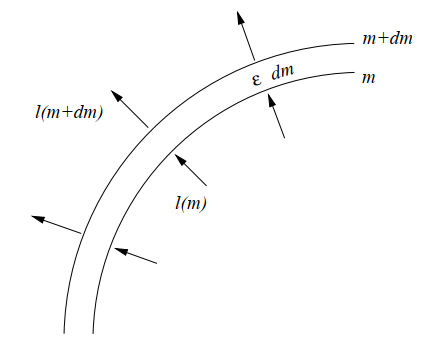
\includegraphics[scale=0.5]{Figures/thermal_equilibrium_scheme.png}
    \caption{Παραγωγή ενέργειας και ροή θερμότητας προς και από σφαιρικό φλοιό μάζας $dm$.}
    \label{fig:thermal_equilibrium_scheme}
\end{figure}

Έστω ότι θεωρούμε έναν σφαιρικό, Λαγκραντζιανό φλοιό σταθερής μάζας $dm$ μέσα σε έναν αστέρα (σχήμα \ref{fig:thermal_equilibrium_scheme}). Αλλαγές στο ποσό θερμότητας ($dQ = dq \,dm$) μπορεί να οφείλονται σε διάφορες πηγές ή καταβόθρες:
\begin{itemize}
    \item Θερμότητα εναποτίθεται από την ενέργεια που παράγουν οι πυρηνικές αντιδράσεις. Ο ρυθμός της ενέργειας ανά μονάδα μάζας και χρόνου είναι $\epsilon_{\text{nuc}}$.
    \item Θερμότητα μπορεί να διαρρέει λόγω ακτινοβολίας νετρίνο, τα οποία δεν αλληλεπιδρούν σχεδόν καθόλου με την ύλη και διαφεύγουν από την επιφάνεια του αστέρα ανεμπόδιστα. Τα νετρίνο δημιουργούνται είτε ως παράγωγα συγκεκριμένων πυρηνικών αντιδράσεων, οπότε και συνυπολογίζονται στην $\epsilon_{\text{nuc}}$, είτε λόγω ασθενών αλληλεπιδράσεων στην περίπτωση που έχουμε πολύ πυκνό και θερμό πλάσμα. Η ενέργεια που χάνεται (ανά μονάδα μάζας και χρόνου) λόγω των νετρίνο συμβολίζεται με $\epsilon_\nu$ και παίζει μεγάλο ρόλο στην ψύξη του πυρήνα σε μεταγενέστερα στάδια της εξέλιξης ενός αστέρα.
    \item Απορρόφηση ή εκπομπή θερμότητας, σύμφωνα με την ισορροπία μεταξύ της θεμικής ροή που εισέρχεται στο κατώτερο μέρος του φλοιού και της θερμικής ροής που εξέρχεται από το ανώτερο στρώμα του φλοιού. Ορίζουμε έτσι ένα νέο μέγεθος, τη \textit{τοπική λαμπρότητα} (local luminosity), ως τον ρυθμό με τον οποίο η ενέργεια με τη μορφή θερμότητας κινείται προς τα εξωτερικά στρώματα διαμέσου μιας σφαίρας ακτίνας $r$. Σε σφαιρική συμμετρία η τοπική λαμπρότητα συνδέεται με την ακτινική ροή ενέργειας $F$ μέσω της σχέσης
    \begin{equation}
        \label{eq:local_luminosity}
        l = 4\pi r^2 F
    \end{equation}
    Έτσι, η τοπική λαμπρότητα στην επιφάνεια του αστέρα είναι $l(R) = L$ και στο κέντρο του $l(0) = 0$. Φυσιολογικά, η θερμότητα ρέει προς τα έξω, προς τη κατεύθυνση δηλαδή που μειώνεται η θερμοκρασία. Γι' αυτό η τοπική λαμπρότητα είναι συνήθως θετική. Παρόλα αυτά, σε συγκεκριμένες περιπτώσεις (π.χ. ψύξη του πυρήνα λόγω ακτινοβολίας νετρίνο), η θερμότητα μπορεί να ρέει προς το εσωτερικό του αστέρα, πράγμα που σημαίνει ότι η τοπική λαμπρότητα είναι αρνητική.
\end{itemize}

Μπορούμε λοιπόν να γράψουμε:
\begin{equation*}
    \delta Q = \epsilon_{\text{nuc}} \,dm \,\delta t - \epsilon_\nu \,dm \,\delta t + l(m) \,\delta t - l(m+dm) \,\delta t
\end{equation*}
Επειδή 
\begin{equation*}
    l(m+dm) = l(m) + \frac{dl}{dm}dm    
\end{equation*}
η παραπάνω σχέση αν διαιρέσουμε και με την μάζα $dm$, γράφεται και ως
\begin{align*}
    \delta q &= \epsilon_{\text{nuc}} \,\delta t - \epsilon_\nu \,\delta t - \frac{dl}{dm} \delta t = \left(\epsilon_{\text{nuc}} - \epsilon_\nu - \frac{dl}{dm}\right) \delta t
\end{align*}
Ο δεύτερος νόμος της θερμοδυναμικής ορίζει την ειδική (specific) εντροπία, $s$, ενός συστήματος ως
\begin{eqnarray}
    \label{eq:second_law_of_thermodynamics}
    dq = Tds
\end{eqnarray}
οπότε παίρνοντας το όριο $\delta t \rightarrow 0$, καταλήγουμε στην σχέση
\begin{eqnarray}
    \label{eq:thermal_equilibrium_lagrangian_with_entropy_term}
    \boxed{\frac{dl}{dm} = \epsilon_{\text{nuc}} - \epsilon_\nu - T \frac{ds}{dt}}
\end{eqnarray}

Συνηθίζεται να γράφουμε 
\begin{equation*}
    \epsilon_{\text{gr}} = -T \frac{ds}{dt}
\end{equation*}
οπότε αν $\epsilon_{\text{gr}} > 0$, τότε ο φλοιός απελευθερώνει ενέργεια λόγω συστολής, ενώ εαν $\epsilon_{\text{gr}} < 0$, ο φλοιός απορροφά ενέργεια λόγω διαστολής. Σε θερμική ισορροπία $\epsilon_{\text{gr}} = 0$, καθώς ο αστέρας είναι σε στατική κατάσταση και άρα η χρονική παράγωγος μηδενίζεται, οπότε έχουμε την απλοποιημένη \textbf{εξίσωση θερμικής ισορροπίας} στο σύστημα συντεταγμένων του Lagrange
\begin{equation}
    \label{eq:thermal_equilibrium_lagrangian_form}
    \boxed{\frac{dl}{dm} = \epsilon_{\text{nuc}} - \epsilon_\nu}
\end{equation}
ή ισοδύναμα, στο σύστημα συντεταγμένων του Euler
\begin{equation}
    \label{eq:thermal_equilibrium_eulerian_form}
    \boxed{\frac{dl}{dr} = 4\pi r^2 \rho \left( \epsilon_{\text{nuc}} - \epsilon_\nu \right)}
\end{equation}
και αποτελεί την τρίτη βασική διαφορική εξίσωση που περιγράφει την δομή ενός αστέρα.

Ολοκληρώνοντας την σχέση \eqref{eq:thermal_equilibrium_lagrangian_form} ως προς τη μάζα, έχουμε
\begin{equation}
    \label{eq:neutrino_luminosity}
    L = \int_{0}^{M} \epsilon_{\text{nuc}} \,dm - \int_{0}^{M} \epsilon_\nu \,dm \equiv L_{\text{nuc}} - L_\nu 
\end{equation}
όπου το $L_\nu$ ορίζει την \textit{λαμπρότητα νετρίνο}. Θεωρώντας ότι $L_\nu \approx 0$, τότε ισχύει $L_{\text{nuc}} = L$, όπως δηλαδή είχαμε υποθέσει ότι ισχύει στην κατάσταση θερμικής ισορροπίας.
%% ---------------------------------------------------------------------------------------------------- %%
%% ---------------------------------------------------------------------------------------------------- %%
%% ---------------------------------------------------------------------------------------------------- %%
\subsection{Πηγές ενέργειας των αστέρων}
Στις αρχές του 20ου αιώνα, η μόνη πηγή παραγωγής ενέργειας ικανή να ερμηνεύσει τη φωτεινότητα του Ήλιου, ήταν η βαρυτική συστολή (η χημική καύση είχε ήδη απορρηφθεί ως ανεπαρκής). Η ιδέα πίσω από αυτόν τον φυσικό μηχανισμό, γνωστός και ως μηχανισμός Kelvin-Helmholtz, είναι το θεώρημα virial. Από όσα αναφέραμε, προκύπτει το συμπέρασμα ότι όταν η ακτίνα ενός αστέρας ελλατώνεται, το ίδιο συμβαίνει και με τη δυναμική του ενέργεια. Συμφωνα όμως με το θεώρημα virial, μόνο η μισή από τη δυναμική ενέργεια που απελευθερώνεται με αυτόν τον τρόπο μένει στον αστέρα με τη μορφή άτακτης κινητικής ενέργειας (θερμότητας). Η υπόλοιπη χάνεται από το σύστημα και ακτινοβολείται στο διάστημα. 
Έστω όμως ότι ο Ήλιος δεν έχει κάποια εσωτερική πηγή ενέργειας και ότι ο μηχανισμός παραγωγής ενέργειας οφείλεται στον μηχανισμό Kelvin-Helmholtz. Κατά τη γέννηση του Ήλιου από το μεσοαστρικό αέριο, είχε μάζα $\mathcal{M}$ και ακτίνα $\mathcal{R}$ αντίστοιχα. Η βαρυτική δυναμική ενέργεια τότε του Ήλιου κατά τη δημουργία του θα ήταν σύμφωνα με τη σχέση \eqref{eq:gravitational_potential_energy}
$$\mathcal{E}_{\text{gr}} = - \frac{3G \mathcal{M}^2}{5 \mathcal{R}}$$
ενώ η ολική ενέργεια σύμφωνα με το θεώρημα virial θα ειναι
$$\mathcal{E}_{\text{tot}} = - \mathcal{E}_{\text{int}} = \frac{1}{2}\mathcal{E}_{\text{gr}} = - \frac{3G \mathcal{M}^2}{10 \mathcal{R}}$$
Επειδή στο αρχικό αυτό στάδιο της δημιουργίας του αστέρα η ακτίνα $\mathcal{R} \rightarrow \infty$, συνεπάγεται ότι $\mathcal{E}_{\text{gr}} \rightarrow \infty$, και άρα η συνολική βαρυτική ενέργεια που έχει ακτινοβολήσει κατά τη διάρκεια της ζωής του μέχρι σήμερα θα είναι
\begin{equation}
    E_{\text{radiated}} = \mathcal{E}_{\text{gr}} - E_{\text{gr}} = \frac{3G M_{\odot}^2}{10 R_{\odot}}
\end{equation}
όπου τα $M_{\odot}, R_{\odot}$ αντιστοιχούν στις σημερινές τιμές. Αντικαθιστώντας αυτές τις τιμές προκύπτει ότι ο Ήλιος από την αρχή της δημιουργίας του μέχρι σήμερα θα είχε ακτινοβολήσει
$$E_{\text{radiated}} \sim 4 \times 10^{48} \,\text{erg}$$
αποκλειστικά λόγω της βαρυτικής συστολής. Υποθέτωντας ότι ακτινοβολούσε όλο αυτό το διάστημα με την ίδια λαμπρότητα $(L_{\odot} = dE/dt)$, μπορούμε να υπολογίσουμε την ηλικία του Ήλιου 
$$t_{\odot} = \frac{E_{\text{radiated}}}{L_{\odot}} \sim 10^7 \,\text{yr}$$

Οι φυσικοί του 20ου αιώνα ήδη ήξεραν, από γεωλογικές μελέτες, πως η ηλικία της Γης είναι περίπου τεσσάρων δισεκατομμυρίων ετών, άρα το παραπάνω αποτέλεσμα για την ηλικία του Ήλιου δεν μπορεί να είναι αληθές. Άρα, η βαρυτική συστολή δεν μπορεί να είναι η μοναδική πηγή ενέργειας των αστέρων. 

Σήμερα γνωρίζουμε πως συγκεκριμένες πυρηνικές αντιδράσεις θα μπορούσαν να λύσουν το πρόβλημα της παραγωγής ενέργειας των αστέρων. Ειδικότερα, η θερμοπυρηνική σύντηξη βασίζεται στην απελευθέρωση της ενέργειας σύνδεσης $Q(Z, N)$, ο οποίος έχει $Z$ πρωτόνια και $N$ νετρόνια
\begin{equation}
    \label{eq:binding_energy}
    Q(Z,N) = \underbrace{\left[ Z m_{\text{p}} + N m_{\text{n}} - m(Z,N) \right]}_{\text{έλλειμα μάζας}}c^2
\end{equation}

Ο μηχανισμός Kelvin-Helmholtz προβλέπει παραγωγή ισχύος σε όλο το εσωτερικό του αστέρα, είναι όμως σημαντικός μόνο στο στάδιο της δημιουργίας του αστέρα από τη συστολή του νέφους σκόνης και αερίου, δηλαδή πριν δημιουργηθούν οι κατάλληλες συνθήκες για τις απαραίτητες πυρηνικές αντιδράσεις. Σε έναν τυπικό αστέρα όπως αυτούς που έχουμε περιγράψει μέχρι στιγμής, η παραγωγή ενέργειας με βαρυτική συστολή είναι μηδενική. Παρόλα αυτά, υπάρχουν στάδια στην εξέλιξη ενός αστέρα όπου ο ρυθμός των πυρηνικών αντιδράσεων μειώνεται και ο μηχανισμός Kelvin-Helmoltz παίζει ενεργό ρόλο στην πορεία που θα ακολουθήσει ο αστέρας.
%% ---------------------------------------------------------------------------------------------------- %%
%% ---------------------------------------------------------------------------------------------------- %%
%% ---------------------------------------------------------------------------------------------------- %%
\subsubsection{Σύντηξη Υδρογόνου}
Το υδρογόνο είναι το στοιχείο με την μεγαλύτερη αφθονία στο σύμπαν και, μαζί με το ήλιο, είναι τα μοναδικά στοιχεία τα οποία έχουν κοσμολογική προέλευση και όχι --μόνο-- αστρική. Είναι λογικό λοιπόν και αναμενόμενο, αν λάβουμε υπόψιν την τεράστια συγκέντρωση του υδρογόνου στα άστρα μάζι με το γεγονός ότι το δυναμικό Coulomb που πρέπει να ξεπεραστεί είναι το ελάχιστο δυνατό, ότι οι αντιδράσεις θα βασίζονται σε πρώτη φάση στη σύντηξη αυτού του στοιχείου. Άρα οι αντιδράσεις που περιμένουμε να δούμε σαν οι πλέον εύκολες είναι οι:

\begin{eqnarray} \rm
p + p & \leftrightharpoons & \rm He^2 \label{eq:p+p_he2} \\ 
\rm p + He^4 & \leftrightharpoons &  \rm Li^5 \label{eq:p+he_li5} \\
\rm He^4 + He^4 & \leftrightharpoons & \rm Be^8 \label{eq:he4+he4_be8_1}
\end{eqnarray}
Παρατηρούμε ότι τα παράγωγα είναι ασταθή και άρα οι αντιδράσεις είναι αμφίδρομες. Άρα χρησιμοποιώντας μόνο τα στοιχεία που βρίσκονται σε αφθονία δεν οδηγηθήκαμε πουθενά. Χρειαζόμαστε λοιπόν έναν μηχανισμό που να επιτρέπει την μετατροπή πρωτονίων σε νετρόνια προκειμένου να οδηγηθούμε σε δημιουργία σταθερών πυρήνων. Ένας τέτοιος μηχανισμός είναι ο εξής:

\begin{eqnarray}
\rm 4p \longrightarrow \rm He^4 + 2e^{+} +2 \nu \label{eq:4p_he4}
\end{eqnarray}

Το πρόβλημα όμως εδώ είναι ότι αυτός ο μηχανισμός απαιτεί την ταυτόχρονη αλληλεπίδραση τεσσάρων πρωτονίων, πράγμα εξαιρετικό απίθανο. Ο σκόπελος αυτός ξεπεράστηκε από τους Bethe και Critchfield (H. Bethe and C. Critchfield, \textit{The formation of deuteron by proton combination}, Phys. Rev., 54:248–254, August 1938) όπου πρότειναν την μετατροπή ενός πρωτονίου σε νετρόνιο μέσω της ασθενούς αλληλεπίδρασης:

\begin{eqnarray}
\rm p + p \longrightarrow \rm d + e^{+} + \nu \label{eq:p+p_d+e}
\end{eqnarray}
Σημειώστε στο σημείο αυτό ότι, επειδή η αλληλεπίδραση αυτή γίνεται με ασθενείς δυνάμεις, η ενεργός διατομή είναι πολύ μικρή ($\sim 10^{-47}$ cm$^2$) --πολλές τάξεις μεγέθους μικρότερη από αυτές που μπορούμε να μετρήσουμε-- και αυτός είναι ο λόγος για τον οποίο το υδρογόνο καταναλώνεται με τόσο αργό ρυθμό στα άστρα (Χ. Ελευθεριάδης, \textit{Πυρηνοσύνθεση: Δημιουργία των Στοιχείων στο Σύμπαν}, Διδακτικές Σημειώσεις, Τμήμα Εκδόσεων Αριστοτέλειου Πανεπιστημίου Θεσσαλονίκης, 2010, pp. 27).

Η σειρά των αντιδράσεων που ορίζονται ως \textbf{κύκλος PPI} είναι:

\begin{eqnarray}
\rm p + p & \longrightarrow & \rm d + e^{+} + \nu  \hspace{1cm} (\times 2) \label{eq:p+p_d+e_twice}\\ 
\rm d + p & \longrightarrow & \rm He^3 + \gamma \hspace{1.5cm} (\times 2) \label{eq:d+p_he3+gamma_twice}\\
\rm He^3 + He^3 & \longrightarrow & \rm He^4 + 2p \label{eq:he3+he3_he4+2p}
\end{eqnarray}
Για θερμοκρασία της τάξης των $T \sim 10^7 \,\text{K}$, οι τυπικοί χρόνοι αντίδρασης είναι 
\begin{itemize}
    \item $14 \times 10^9 \,\text{yr}$ για την \eqref{eq:p+p_d+e_twice}
    \item $6 \,\text{s}$ για την \eqref{eq:d+p_he3+gamma_twice}
    \item $10^6 \,\text{yr}$ για την \eqref{eq:he3+he3_he4+2p}
\end{itemize}
Ο συνολικός λοιπόν ρυθμός με τον οποίο τέσσερα πρωτόνια μετατρέπονται σε ήλιο, καθορίζεται από την αρχική αντίδραση δύο πρωτονίων προς δευτέριο (bottleneck). Προσεγγιστικά, η ενέργεια που παράγεται από τον κύκλος PPI είναι
\begin{eqnarray}
    \label{eq:ppi_energy}
    \epsilon_{\text{PP}} \propto \rho \,X_{\text{H}}^2 \,T^4 
\end{eqnarray}
Η ισχυρή εξάρτηση από την θερμοκρασία είναι ο λόγος που αυτού του είδους οι αντιδράσεις χαρακτηρίζονται ως "θερμοπυρηνικές".
%% ---------------------------------------------------------------------------------------------------- %%
%% ---------------------------------------------------------------------------------------------------- %%
%% ---------------------------------------------------------------------------------------------------- %%   
\subsubsection{Καύση Δευτέριου}
Είδαμε λοιπόν ότι, το δευτέριο δημιουργείται στο εσωτερικό των αστέρων κατά βάση μέσω της αντίδρασης \eqref{eq:p+p_d+e_twice}. Η ποσότητα του δευτερίου που παράγεται είναι πολύ λίγη και το επόμενο στάδιο είναι η καύση του μέσω διάφορων αντιδράσεων είτε με πρωτόνια, είτε με άλλους πυρήνες δευτερίου είτε ακόμα και με πυρήνες ηλίου. Όμως σε ένα αστρικο περιβάλλον, η συγκέντρωση των πρωτονίων υπερτερεί κατά πολύ έναντι οποιουδήποτε άλλου είδους σωματιδίων και έχοντας κατά νου ότι ο ρυθμός αντίδρασης εξαρτάται, μεταξύ άλλων, και από το πλήθος των σωματιδίων, είναι εύλογο να υποθέσουμε ότι η καταστροφή του δευτερίου συμβαίνει μέσω της αντίδρασης:

\begin{eqnarray}
\rm d + p \longrightarrow \rm He^3 + \gamma \label{eq:d+p_he3+gamma}
\end{eqnarray}

Οι πυρήνες $^3$He που δημιουργούνται με αυτό τον τρόπο, συμβάλλουν ακόμα περισσότερο στην καταστροφή του δευτερίου μέσω των αντιδράσεων:

\begin{eqnarray}
\rm d + He^3 & \longrightarrow & \rm He^4 + p \label{eq:d+he3_he4+p}\\
\rm d + He^3 & \longrightarrow & \rm Li^5 + \gamma \label{eq:d+he3_li5+gamma}
\end{eqnarray}
Η συμβολή της \eqref{eq:d+he3_he4+p} στην καύση του δευτερίου είναι σημαντικότερη από αυτή της \eqref{eq:d+he3_li5+gamma} λόγω του ότι η ενεργός διατομή της είναι μεγαλύτερη\footnote{Η ενεργός διατομή της \eqref{eq:d+he3_he4+p} είναι ακόμα μεγαλύτερη και από αυτή της \eqref{eq:d+p_he3+gamma} όμως λόγω της ποσότητας των πρωτονίων, που είναι εξαιρετικά μεγάλος, η \eqref{eq:d+p_he3+gamma} είναι ο κύριος μηχανισμός καύσης του δευτερίου.}.

Τελικώς, επειδή η καύση του δευτερίου λαμβάνει χώρα πριν το άστρο καταφέρει να φτάσει στην κύρια ακολουθία, και λόγω του ότι η συγκέντρωση του δευτερίου είναι τόσο μικρή που γρήγορα θα καταναλωθεί, η μόνη συνέπεια είναι μία επιβράδυνση της κατάρρευσης του άστρου.
%% ---------------------------------------------------------------------------------------------------- %%
%% ---------------------------------------------------------------------------------------------------- %%
%% ---------------------------------------------------------------------------------------------------- %%
\subsubsection{Οι κύκλοι πρωτονίου-πρωτονίου}
Μέχρι στιγμής, αναφέραμε τον πρώτο κύκλο πρωτονίου-πρωτονίου (PPI) όπου στην τελευταία εξίσωση είχαμε την αντίδραση δύο πυρήνων He$^3$. Αντί γι' αυτήν την αντίδραση, μπορούμε να έχουμε την:

\begin{eqnarray}
\rm He^3 + He^4 \longrightarrow \rm Be^7 + \gamma \label{eq:he3+he4_be7+gamma}
\end{eqnarray}
και με τη σειρά του, το Be$^7$:

\begin{eqnarray}
\rm Be^7 + e & \longrightarrow & \rm Li^7 + \nu \label{eq:be7+e_li7+nu}\\
\rm Li^7 + p & \longrightarrow & \rm He^4 + \alpha \label{eq:li7+p_he4+alpha}
\end{eqnarray}
Παρατηρούμε ότι ο κύκλος αυτός, που είναι γνωστός ως \textbf{κύκλος PPII}, οδηγεί ξανά στη δημιουργία He$^4$, ενώ το Be$^7$ και το Li$^7$ δρουν απλά ως καταλύτες δεδομένου ότι δημιουργούνται και καταστρέφονται κατά τον κύκλο αυτό.

Τέλος, υπάρχει περίπτωση το Be$^7$ να αλληλεπιδράσει με ένα πρωτόνιο, πριν προλάβει να κάνει αρπαγή ηλεκτρονίου μέσω της \eqref{eq:be7+e_li7+nu}. Σε αυτή την περίπτωση έχουμε τον εξής κύκλο:

\begin{eqnarray}
\rm Be^7 + p & \longrightarrow & \rm B^8 + \gamma \label{eq:be7+p_b8+gamma}\\
\rm B^8 & \longrightarrow & \rm Be^8 + e^{+} + \nu \label{eq:b8_be8+e+nu}\\
\rm Be^8 & \longrightarrow & \rm He^4 + He^4 \label{eq:be8_he4+he4}
\end{eqnarray}
Αυτός ο κύκλος είναι γνωστός ως \textbf{κύκλος PPIII}. Παρατηρούμε ότι και εδώ το βηρύλλιο και το βόριο παίζουν το ρόλο καταλύτη.
%% ---------------------------------------------------------------------------------------------------- %%
%% ---------------------------------------------------------------------------------------------------- %%
%% ---------------------------------------------------------------------------------------------------- %%
\subsubsection{Ο κύκλος άνθρακα}
Θα περίμενε κανείς, ότι βαρύτερα στοιχεία όπως ο άνθρακας, το οξυγόνο κτλ, θα έπρεπε να έχουν μηδενική συγκέντρωση κατά τα πρώτα στάδια εξέλιξης ενός άστρου, της καύσης δηλαδή του υδρογόνου και του ηλίου. Σε γενικές γραμμές αυτό αληθεύει και η σύγκεντρωση αυτών των στοιχείων αρχίζει να γίνεται σημαντική μετά την ολοκλήρωση της καύσης του ηλίου, όμως πολλά άστρα περιέχουν τέτοια βαρύτερα στοιχεία τα οποία βρίσκονταν σε πρωτοαστρικά νέφη προερχόμενα από την εκρηκτική κατάληξη άλλων άστρων. Τα στοιχεία αυτά μπορούν να συμμετέχουν στους κύκλους των πυρηνικών καύσεων μέσω των αντιδράσεων:

\begin{eqnarray}
\rm C^{12} + p & \longrightarrow & \rm N^{13} + \gamma \label{eq:c12+p_n13+gamma}\\
N^{13} & \longrightarrow & C^{13} + e^{+} + \nu \label{eq:n13_c13+e+nu}
\end{eqnarray}

και 

\begin{eqnarray}
\rm C^{13} + p & \longrightarrow & \rm N^{14} + \gamma \label{eq:c13+p_n14+gamma}\\
\rm N^{14} + p & \longrightarrow & \rm O^{15} + \gamma \label{eq:n14+p_o15+gamma}\\     
\rm O^{15} & \longrightarrow & \rm N^{15} + e^{+} + \nu \label{eq:o15_n15+e+nu}\\
\rm N^{15} + p & \longrightarrow & \rm C^{12} + He^4 \label{eq:n15+p_c12+he4}
\end{eqnarray}
ή συνολικά:

\begin{eqnarray}
\rm C^{12} + 4p \longrightarrow \rm C^{12} + He^4 + 2e^{+} + 2 \nu \label{eq:c12+4p_c12+he4+2e+2nu}
\end{eqnarray}
όπου ο άνθρακας είναι απλά καταλύτης. Αυτός ο κύκλος είναι γνωστός ως \textbf{κύκλος άνθρακα} ή κύκλος CNO, όπου χρησιμοποιώντας ισότοπα άνθρακα, αζώτου ή οξυγόνου ως καταλύτες, παίρνουμε ήλιο-4, δύο ποζιτρόνια και δύο νετρίνο. Ο ίδιος κύκλος ισχύει για οποιοδήποτε από τα στοιχεία C, N, O κι αν θεωρήσουμε ως αρχικά παρόν αν και η παρουσία οξυγόνου περιπλέκει κάπως τα πράγματα οδηγώντας μας στον διπλό κύκλο CNO αλλά αυτό είναι ένα θέμα που δεν θα αναπτύξουμε εδώ.

Η ενέργεια που παράγεται μέσω του κύκλου άνθρακα είναι προσεγγιστικά
\begin{eqnarray}
    \label{eq:cno_energy}
    \epsilon_{\text{CNO}} \propto \rho \,X_{\text{H}} \,X_{\text{CNO}} \,T^{20} 
\end{eqnarray}
Παρατηρούμε ότι η ενέργεια που παράγεται μέσω αυτής της διαδικασίας έχει εξαιρετικά μεγάλη εξάρτηση από τη θερμοκρασία και ότι ακόμα και μικρές μεταβολές $\Delta T$, μπορεί να οδηγήσουν στην εξάλειψη αυτής της πηγής ενέργειας.
%% ---------------------------------------------------------------------------------------------------- %%
%% ---------------------------------------------------------------------------------------------------- %%
%% ---------------------------------------------------------------------------------------------------- %%
\subsubsection{Καύση Ηλίου}
Το ήλιο είναι, όπως έχουμε αναφέρει, το δεύτερο σε αφθονία στοιχείο στο Σύμπαν και έχει προέλευση τόσο κοσμολογική όσο και αστρική, μέσω των αντιδράσεων που παρουσιάσαμε στις προηγούμενες παραγράφους. Όταν λοιπόν τελειώσει η φάση της καύσης του υδρογόνου, η υδροστατική ισορροπία θα χαθεί λόγω της συνεχούς μείωσης της βαθμίδας της πίεσης και δεν θα υπάρχει τίποτα να αντισταθμίσει την βαρυτική κατάρρευση του άστρου. Έτσι, το άστρο θα συνεχίσει να καταρρέει μέχρις ότου η θερμοκρασία και η πίεση στο εσωτερικό του να επιτρέψουν την εκκίνηση των πυρηνικών μετασχηματισμών με βάση το ήλιο. Ο ρόλος του θεωρήματος virial και του μηχανισμού Kelvin-Helmholtz σε αυτό το στάδιο, δηλαδή μέχρι την εκκίνηση της καύσης του ηλίου, είναι προφανής.

Το πρόβλημα εδώ είναι, όπως αναφέρει ο Clayton, ότι δεν υπάρχουν σταθεροί πυρήνες με μαζικό αριθμό 5 και 8. Το γεγονός αυτό, απαγορεύει τόσο την σύντηξη δύο πυρήνων ηλίου μεταξύ τους όσο και την αντίδραση ενός άλφα σωματιδίου με κάποιο νουκλεόνιο. Επίσης, ο άνθρακας και το οξυγόνο (τα δύο στοιχεία που βρίσκονται σε μεγαλύτερη αφθονία μετά το ήλιο) είναι συνθέσεις τριών και τεσσάρων πυρήνων ηλίου αντίστοιχα, αλλά η αντίδραση πολλών σωματιδίων ταυτόχρονα είναι εξαιρετικά απίθανη και δεν δικαιολογεί την παρατηρούμενη αναλογιά αυτών των στοιχείων.

Εν συντομία, το πρόβλημα προσεγγίστηκε μέσω της σχέσης
\begin{eqnarray}
\rm He^4 + He^4 \leftrightharpoons \rm Be^8 \label{eq:he4+he4_be8}
\end{eqnarray}    
όπου φαίνεται ότι η αντίδραση δύο πυρήνων ηλίου δίνει το ασταθές βηρύλλιο-8. Όμως λόγω της συνεχούς δημιουργίας και καταστροφής του βηρυλλίου καθώς και του μέσου χρόνου διάσπασής του ($\sim 2.6 \times 10^{-16} \,\text{sec}$, θα υπάρχει μία ισορροπία έτσι ώστε κάθε χρονική στιγμή να υπάρχει ένας ικανοποιητικός αριθμός πυρήνων Be$^8$, έτσι ώστε να είναι πιθανή η αντίδραση:

\begin{eqnarray}
\rm Be^8 + He^4 \longrightarrow \rm C^{12} + \gamma \label{eq:be8+he4_c12+gamma}
\end{eqnarray}
η οποία παρουσιάζει κάποια χαρακτηριστικά συντονισμού.
%% ---------------------------------------------------------------------------------------------------- %%
%% ---------------------------------------------------------------------------------------------------- %%
%% ---------------------------------------------------------------------------------------------------- %%
\subsubsection{Η διαδικασία τριών-$\alpha$}
Η διαδικασία τριών-$\alpha$ είναι αυτή κατά την οποία τρεις πυρήνες ηλίου μετασχηματίζονται μέσω σύντηξης σ' ένα πυρήνα άνθρακα. Όπως αναφέρθηκε και πριν, η πιθανότητα να συμβεί μία τέτοια αντίδραση είναι εξαιρετικά μικρή και έτσι απαιτείται μεγάλο χρονικό διάστημα για να παραχθεί σημαντική ποσότητα άνθρακα μέσω αυτής. Μπορούμε εν γένει να θεωρήσουμε τις εξισώσεις \eqref{eq:he4+he4_be8} και \eqref{eq:be8+he4_c12+gamma} ως μία διαδικασία τριών-$\alpha$ δύο βημάτων. Η ενέργεια που παράγεται μέσω αυτής της διαδικασίας είναι προσεγγιστικά
\begin{eqnarray}
    \label{eq:triple_alpha_energy}
    \epsilon_{\text{3\alpha}} \propto \rho^2 \,X_{\text{He}}^3 \,T^{30} 
\end{eqnarray}

Έχοντας λύσει το πρόβλημα της δημιουργίας του άνθρακα μέσω της τριών-$\alpha$ διαδικασίας, μπορούμε να υποθέσουμε ότι το οξυγόνο σχηματίζεται μέσω της αντίδρασης:

\begin{eqnarray}
\rm C^{12} +He^4 \longrightarrow \rm O^{16} + \gamma \label{eq:c12+he4_o16+gamma}
\end{eqnarray}
και ακόμα, με ένα βήμα παραπάνω έχουμε το σχηματισμό ενός πυρήνα νέον-20 μέσω της:

\begin{eqnarray}
\rm O^{16} + He^4 \longrightarrow \rm Ne^{20} + \gamma \label{eq:o16+he4_ne20+gamma}
\end{eqnarray}

Περαιτέρω αντιδράσεις είναι σχετικά απίθανες λόγω του αυξημένου φράγματος Coulomb. Σε γενικές γραμμές, λαμβάνοντας υπόψιν τις πιθανότητες να συμβούν οι παραπάνω αντιδράσεις, είναι ασφαλές να πούμε ότι το αποτέλεσμα της καύσης του He$^4$ είναι ο σχηματισμός του άνθρακα και του οξυγόνου.
%% ---------------------------------------------------------------------------------------------------- %%
%% ---------------------------------------------------------------------------------------------------- %%
%% ---------------------------------------------------------------------------------------------------- %%
\subsubsection{Καύση Άνθρακα}
Ο αστέρας, έχοντας εξαντλήσει και τα αποθέματα του He$^4$, έχει απομείνει με τεράστιες συγκεντρώσεις άνθρακα-12 και οξυγόνο-16 στο εσωτερικό του. Για ακόμα μια φορά υπερισχύει η βαρυτική κατάρρευση του άστρου μέχρις ότου η θερμοκρασία στο κέντρο του να φτάσει την τάξη του $\sim 10^9 \,\text{K}$. Στο σημείο αυτό ξεκινούν οι αντιδράσεις μεταξύ πυρήνων άνθρακα και ακολουθούν αυτές που περιλαμβάνουν το οξυγόνο.
Από μία πληθώρα πυρηνικών αντιδράσεων μεταξύ δύο πυρήνων άνθρακα, οι πιο πιθανές να συμβούν είναι οι:

\begin{eqnarray}
\rm C^{12} + C^{12} & \longrightarrow & \rm  ^{24}Mg^{*} \longrightarrow Ne^{20} + \alpha + (4.6 \,\text{MeV}) \label{eq:c12+c12_mg24_ne20+alpha+q}\\
\rm C^{12} + C^{12} & \longrightarrow & \rm Na^{23} + p + (2.2 \,\text{MeV}) \label{eq:c12+c12_na23+p+q}
\end{eqnarray}

Αντιδράσεις μεταξύ άνθρακα και άλλων στοιχείων όπως οξυγόνο ή νέον δεν αποκλείονται, ειδικά κατά το τελευταίο στάδιο καύσης του άνθρακα, αλλά δεν κατέχουν σημαντικό ρόλο. Με παρόμοιο τρόπο γίνεται και η καύση του οξυγόνου μέσω των:

\begin{eqnarray}
\rm O^{16} + O^{16} & \longrightarrow & \rm S^{32} + \gamma  \label{eq:o16+o16_s32}\\
\rm O^{16} + O^{16} & \longrightarrow & \rm S^{31} + n \label{eq:o16+o16_s31+n}\\
\rm O^{16} + O^{16} & \longrightarrow & \rm P^{31} + p \label{eq:o16+o16_p31+p}\\
\rm O^{16} + O^{16} & \longrightarrow & \rm Si^{31} + \alpha \label{eq:o16+o16_si31+alpha}
\end{eqnarray}

Τέλος, το υπάρχον Ne$^{20}$ μπορεί να συντελέσει στην παραγωγή ενέργειας σε έναν αστέρα, για πολύ σύντομο χρονικό διάστημα ( $\sim 1 \,\text{yr}$), κυρίως μέσω αντιδράσεων φωτοδιάσπασης στις οποίες θα αναφερθούμε παρακάτω.
%% ---------------------------------------------------------------------------------------------------- %%
%% ---------------------------------------------------------------------------------------------------- %%
%% ---------------------------------------------------------------------------------------------------- %%
\subsubsection{Καύση Πυριτίου}
Μετά το τέλος της καύσης του οξυγόνου, ο πυρήνας του άστρου αποτελείται κυρίως από πυρίτιο-28. Φυσικά, το άστρο θα ακολουθήσει πάλι την γνωστή πορεία που περιλαμβάνει την συστόλη του με ταυτόχρονη αύξηση της θερμοκρασίας και της πίεσης στο εσωτερικό του, οπότε θα περίμενε κανείς να συναντήσει αντιδράσεις μεταξύ των πυρήνων πυριτίου. Κάτι τέτοιο δεν συμβαίνει όμως καθώς πριν προλάβουν να αναπτυχθούν οι κατάλληλες θερμοκρασίες, ξεκινάει η διαδικασία της \textbf{φωτοδιάσπασης} (φωτόνια τα οποία διασπούν τους πυρήνες με τους οποίους αντιδρούν) που καταστρέφει το υπάρχον πυρίτιο και διαδραματίζει ουσιαστικό λόγο στην συγκεκριμένη φάση της πυρηνοσύνθεσης.
Οι φωτοδιασπάσεις δίνουν σαν αποτέλεσμα εκπομπή σωματιδίων-α, πρωτονίων και νετρονίων και με αυτό τον τρόπο, μέσα από πολύπλοκες αντιδράσεις, οδηγούν στην δημιουργία της ονομαζόμενης \textbf{ομάδας του Fe $^{56}$} και τις αντίστοιχες ισοτοπικές αναλογίες που συναντάμε. Φαίνεται λοιπόν πως η αλυσίδα της σύνθεσης νέων στοιχείων στην καρδιά των αστέρων σπάει με τον σχηματισμό του σιδήρου. Για τον σχηματισμό χημικών στοιχείων και τις διαδικασίες που απαιτούνται, γίνεται αναφορά στο παράρτημα \ref{apx:nucleosynthesis}.

Να σημειώσουμε εδώ ότι, ο σχηματισμός των ελαφρών στοιχείων (Li, Be, B) καθώς και οι κοσμικές τους αναλογίες, δεν δικαιολογούνται από τους μηχανισμούς που περιγράψαμε μέχρι στιγμής. Αυτό συμβαίνει γιατί τα ισότοπα αυτά καταστρέφονται στις συνθήκες που επικρατούν στο εσωτερικό των αστέρων. Στο πρόβλημα αυτό θα αναφερθούμε στο παράρημα \ref{apx:nucleosynthesis}, στο υποκεφάλαιο της l-διεργασίας.
%% ---------------------------------------------------------------------------------------------------- %%
%% ---------------------------------------------------------------------------------------------------- %%
%% ---------------------------------------------------------------------------------------------------- %%
\subsection{Χαρακτηριστικοί χρόνοι}
Υπάρχουν τρεις σημαντικές χρονικές κλίμακες όταν συζητάμε την αστρική εξέλιξη. Αυτές οι χρονικές κλίμακες σχετίζονται με αλλαγές στη μηχανική δομή ενός αστέρα (που περιγράφεται από την εξίσωση κίνησης \eqref{eq:equation_of_motion_eulerian_coordinate}), με αλλαγές στη θερμική δομή του αστέρα (που περιγράφονται από το θεώρημα virial), και αλλαγές στη χημική σύσταση του αστέρα.
%% ---------------------------------------------------------------------------------------------------- %%
%% ---------------------------------------------------------------------------------------------------- %%
%% ---------------------------------------------------------------------------------------------------- %%
\subsubsection{Δυναμική χρονική κλίμακα}
Μπορούμε να αναρωτηθούμε τι θα γίνει αν η κατάσταση υδροστατικής ισορροπίας παραβιαστεί: πόσο γρήγορα θα συμβούν αλλαγές στη δομή του αστέρα; Η απάντηση δίνεται από την εξίσωση κίνησης \eqref{eq:equation_of_motion_eulerian_coordinate}. Για παράδειγμα, ας υποθέσουμε ότι η πίεση που υποστηρίζει τον αστέρα ενάντια στην βαρύτητα ξαφνικά μηδενίζεται. Όλοι οι σφαιρικοί φλοιοί τότε επιταχύνονται προς το κέντρο του αστέρα λόγω της βαρύτητας: ο αστέρας ξεκινάει να καταρρέει σε συνθήκες ελεύθερης πτώσης (free fall). Προσεγγιστικά μπορούμε να γράψουμε
\begin{align*}
    \left| \ddot{r} \right| &= - \frac{GM}{r^2} - \frac{1}{\rho} \cancelto{0}{\frac{dP}{dr}} = - g 
    \Rightarrow \frac{d^2r}{dt^2} = -g \longrightarrow \left| r \right| \approx \frac{1}{2} gt^2 
    \longrightarrow \tau_{\text{ff}} = \sqrt{\frac{2R^3}{GM}}
\end{align*}
Θεωρώντας την πυκνότητα σταθερή, $\langle \rho \rangle = \frac{3M}{4\pi R^3}$ η παραπάνω σχέση γράφεται και ως
\begin{eqnarray}
    \label{eq:dynamic_timescale}
    \tau_{\text{dyn}} = \sqrt{\frac{2R^3}{GM}} \approx  \frac{1}{2} (G \langle \rho \rangle)^{- \frac{1}{2}}
\end{eqnarray}
Φυσικά κάθε σφαιρικός φλοιός επιταχύνεται με διαφορετικό ρυθμό, οπότε η παραπάνω εκτίμηση πρέπει να εκλαμβάνεται ως μία μέση τιμή για την οποία ο αστέρας καταρρέει σε μία απόσταση $R$. Μία άλλη εκτίμηση για τον δυναμικό χρόνο μπορεί να γίνει με παρόμοιο τρόπο, θεωρώντας πως η βαρύτητα ξαφνικά εξαφανίζεται: αυτό θα μας δώσει τον χρόνο που χρειάζεται η πίεση για να διαλύσει τον αστέρα, ο οποίος είναι παρόμοιος με τον χρόνο που χρειάζεται ένα ακουστικό κύμα (άλλωστε η πίεση σχετίζεται με τα ακουστικά κύματα) να ταξιδέψει από το κέντρο μέχρι την επιφάνεια του αστέρα.

Για τον Ήλιο, προκύπτει ότι $\tau_{\text{dyn}} \approx 1600 \,\text{s}$, ή περίπου μισή ώρα. Το αποτέλεσμα αυτό έχει κάποια πολύ σημαντικά αποτελέσματα:
\begin{itemize}
    \item Οποιαδήποτε απομάκρυνση από την κατάσταση υδροστατικής ισορροπίας, πρέπει να οδηγήσει πολύ γρήγορα σε παρατηρήσιμα φαινόμενα: είτε συστολή είτε διαστολή στον δυναμικό χρόνο. Αν ο αστέρας δεν μπορεί να επανέλθει σε κατάσταση υδροστατικής ισορροπίας, θα οδηγηθεί είτε σε κατάρρευση είτε σε έκρηξη.
    \item Φυσιολογικά, η υδροστατική ισορροπία μπορεί να επανέλθει έπειτα από κάποια διαταραχή (dynamical stability). Παρόλα αυτά, διαταραχή στην υδροστατική ισορροπία μπορεί να οδηγήσει σε ταλαντώσεις μικρής κλίμακας στον δυναμικό χρόνο. Αυτές οι ταλαντώσεις έχουν παρατηρηθεί τόσο στον Ήλιο όσο και σε άλλους αστέρες, με μια περίοδο της τάξης των λεπτών στην περίπτωση του Ήλιου. Η εξίσωση \eqref{eq:dynamic_timescale} μας δείχνει ότι η περίοδος των αναπάλσεων αποτελεί ένα προσεγγιστικό μέτρο της μέσης πυκνότητας του αστέρα.
    \item Πέρα από τις όποιες ταλαντώσεις, οι αστέρες βρίσκονται εξαιρετικά κοντά σε μία κατάσταση υδροστατικής ισορροπίας αφού οποιαδήποτε διαταραχή αποσβήνεται αμέσως. Μπορούμε λοιπόν με βεβαιότητα να θεωρήσουμε πως η εξίσωση \eqref{eq:hydrostatic_equilibrium_lagrangian_coordinate} ισχύει για το μεγαλύτερο χρονικό διάστημα της ζωής τους. Οι αστέρες εξελίσσονται και γι' αυτό το λόγο δεν μπορούν να είναι εντελώς στατικοί, αλλά οι αλλαγές συμβαίνουν εξαιρετικά αργά συγκριτικά με τον δυναμικό χρόνο. Έτσι, μπορούμε να πούμε ότι εξελίσσονται ημι-στατικά (quasi-statically), δηλαδή μέσω μιας σειράς σχεδόν-τέλειων καταστάσεων υδροστατικής ισορροπίας.
\end{itemize}
%% ---------------------------------------------------------------------------------------------------- %%
%% ---------------------------------------------------------------------------------------------------- %%
%% ---------------------------------------------------------------------------------------------------- %%
\subsubsection{Θερμική χρονική κλίμακα}
Ο δεύτερος χαρακτηριστικός χρόνος περιγράφει το πόσο γρήγορα μπορούν να εμφανιστούν αλλαγές στην θερμική δομή ενός αστέρα. Συνεπάγεται λοιπόν πως είναι και η χρονική κλίμακα στην οποία ένας αστέρας ο οποίος βρίσκεται σε θερμική ισορροπία αντιδρά όταν αυτή η ισορροπία διαταράσσεται. Για να έχουμε μία εκτίμηση του μεγέθους αυτής της χρονικής κλίμακας, στρεφόμαστε στο θεώρημα virial. Είδαμε ότι ένας αστέρας χωρίς κάποια εσωτερική πηγή ενέργειας συστέλλεται ακτινοβολώντας την εσωτερική του ενέργεια:
$$L = \dot{E}_{\text{int}} = - \frac{1}{2} \dot{E}_{\text{gr}}$$
όπου η τελευταία ισότητα ισχύει για την περίπτωση του ιδανικού αερίου.
Αυτό σημαίνει ότι μπορούμε να γράψουμε
\begin{equation*}
    L = \frac{d E_{\text{int}}}{dt} = - \frac{1}{2} \frac{d E_{\text{gr}}}{dt} \longrightarrow \tau_{\text{KH}} = \frac{E_{\text{int}}}{L} = - \frac{1}{2} \frac{E_{\text{gr}}}{L}
\end{equation*}
και επειδή η βαρυτική δυναμική ενέργεια είναι, όπως έχουμε δείξει, $E_{\text{gr}} = - \frac{3GM^2}{5R}$, η παραπάνω σχέση γράφεται
\begin{equation}
    \label{eq:thermal_timescale}
    \tau_{\text{KH}} = \frac{3GM^2}{10RL} \simeq 1.5 \times 10^7 \left( \frac{M}{M_{\odot}} \right)^2 \left( \frac{R}{R_{\odot}} \right)^{-1} \left( \frac{L}{L_{\odot}} \right)^{-1} \,\text{yr}
\end{equation}
Η ποσότητα $\tau_{\text{KH}}$ εκφράζει την θερμική χρονική κλίμακα (ή κλίμακα Kelvin-Helmholtz), και εκφράζει τον χρόνο στον οποίο θα λάμβανε χώρα μία τέτοια συστολή. Για τον Ήλιο είδαμε ότι $\tau_{\text{KH}} \sim 10^7 \,\text{yr}$, που σημαίνει ότι είναι πολλές τάξεις μεγέθους μεγαλύτερη από τον δυναμικό χρόνο. Γι' αυτό το λόγο δεν υπάρχει κάποια άμεση παρατήρηση που να αποδεικνύει ότι ένας οποιοσδήποτε αστέρας βρίσκεται όντως σε κατάσταση θερμικής ισορροπίας. Οι πυρηνικές αντιδράσεις που συμβαίνουν στο κέντρο του αστέρα θα του επέτρεπαν παρόλα αυτά να βρεθεί όντως σε μία τέτοια κατάσταση. Πολλές φάσεις στην εξέλιξη ενός αστέρα, κατά τη διάρκεια των οποίων η ισχύς των πυρηνικών αντιδράσεων είναι είτε μηδενική είτε ελλιπής, λαμβάνουν χώρα σε αυτή τη θερμική χρονική κλίμακα.
%% ---------------------------------------------------------------------------------------------------- %%
%% ---------------------------------------------------------------------------------------------------- %%
%% ---------------------------------------------------------------------------------------------------- %%
\subsubsection{Πυρηνική χρονική κλίμακα}
Ένας αστέρας μπορεί να παραμείνει σε θερμική ισορροπία για όσο διάστημα το επιτρέπει το απόθεμα των πυρηνικών καυσίμων του. Η χρονική κλίμακα στην οποία εξαντλούνται τα αποθέματα του εκάστοτε πυρηνικού αποθέματος, ονομάζεται πυρηνική χρονική κλίμακα. Επειδή κατά τη διάρκεια αυτών των αντιδράσεων, ένα στοιχείο μετατρέπεται σε κάποιο άλλο (π.χ. υδρογόνο σε ήλιο), είναι επίσης η χρονική κλίμακα στην οποία αλλάζει η χημική σύσταση του εσωτερικού του αστέρα.

Η πηγή ενέργειας της θερμοπυρηνικής σύντηξης είναι η μετατροπή μέρους της μάζας των αντιδρώντων σωματιδίων σε ενέργεια, έτσι ώστε $E_{\text{nuc}} = \Delta m \,c^2$, όπου $\Delta m$ το έλλειμα μάζας.
Σε κατάσταση θερμικής ισορροπίας ισχύει
$$L = L_{\text{nuc}} = \dot{E}_{\text{nuc}} = \frac{d E_{\text{nuc}}}{dt}$$
έτσι ώστε η πυρηνική χρονική κλίμακα να ορίζεται ως
\begin{equation}
    \label{eq:nuclear_timescale}
    \tau_{\text{nuc}} = \frac{E_{\text{nuc}}}{L} = \eta f_{\text{c}} X \frac{M c^2}{L} = \eta X \frac{M_{\text{c}} c^2}{L}
\end{equation}
όπου $\eta$ είναι ένας παράγοντας απόδοσης της θερμοπυρηνικής σύντηξης (για το υδρογόνο $\eta \sim 0.7 \,\%$), $f_{\text{c}}$ είναι το ποσοστό της μάζας του αστέρα στο οποίο πραγματοποιούται αντιδράσεις (για άστρα σαν τον Ήλιο είναι $\sim 10 \,\%$), $X$ η αφθονία του υδρογόνου, και $M$ η συνολική μάζα του αστέρα. Με $M_{\text{c}}$ συμβολίζουμε τη μάζα του πυρήνα του αστέρα, δηλαδή τη μάζα εκείνη που συμμετέχει στις πυρηνικές αντιδράσεις.

Για τον Ήλιο, $\tau_{\text{nuc}} \sim 10^{10} \,\text{yr}$ που είναι τάξεις μεγέθους μεγαλύτερη από την θερμική χρονική κλίμακα. Άρα, η υπόθεση ότι τα αστέρια μπορούν να φτάσουν μία κατάσταση θερμικής ισορροπίας είναι βάσιμη.

Γενικά λοιπόν ισχύει
\begin{equation}
    \label{eq:stellar_timescales_order}
    \tau_{\text{nuc}} \gg \tau_{\text{KH}} \gg \tau_{\text{dyn}}
\end{equation}
Ως αποτέλεσμα, ο ρυθμός των πυρηνικών αντιδράσεων καθορίζει το βήμα της αστρικής εξέλιξης, και οι αστέρες μπορεί να θεωρηθεί ότι βρίσκονται σε υδροστατική και θερμική ισορροπία για το μεγαλύτερο μέρος της ζωής τους.
%% ---------------------------------------------------------------------------------------------------- %%
%% ---------------------------------------------------------------------------------------------------- %%
%% ---------------------------------------------------------------------------------------------------- %%
\subsection{Διάδοση ενέργειας στους αστέρες}
Η διάδοση της ενέργειας σε ένα φυσικό σύστημα μπορεί να γίνει γενικά με τρεις τρόπους: με \textbf{αγωγή} (conduction), με \textbf{ρεύματα μεταφοράς} (convection) ή με \textbf{ακτινοβολία} (radiation). Ο συντελεστής θερμικής αγωγιμότητας των αερίων, όταν η πίεσή τους δεν είναι εξαιρετικά μεγάλη, είναι μηδαμινός. Έτσι, με εξαίρεση τους πυρήνες των πολύ μεγάλων, σε μάζα, αστέρων, των λευκών νάνων και των αστέρων νετρονίων, όπου η πίεση παίρνει ακραίες τιμές, θεωρούμε ότι η διάδοση ενέργειας μέσω αγωγής δεν είναι σημαντική συγκριτικά με τους άλλους δύο τρόπους. Επειδή οι μικροφυσικές διεργασίες στις οποίες βασίζονται οι δύο αυτοί τρόποι είναι εντελώς διαφορετικές, δεν πρέπει να μας εκπλήσσει το γεγονός ότι και η μακροσκοπική μαθηματική τους περιγραφή οδηγεί σε δύο διαφορικές εξισώσεις με εντελώς διαφορετική μαθηματική δομή.

Τα ρεύματα μεταφοράς είναι ο κύριος τρόπος διάδοσης της ενέργειας στους ψυχρούς αστέρες φασματικού τύπου Κ και Μ, συνεισφέρει όμως λιγότερο σε αστέρες όπως ο Ήλιος και σχεδόν καθόλου σε αστέρες προγενέστερου φασματικού τύπου. Η ακτινοβολία είναι ο κύριος τρόπος διάδοσης της ενέργειας στους θερμούς αστέρες καθώς και στα βαθύτερα στρώματα των ψυχρών αστέρων.
%% ---------------------------------------------------------------------------------------------------- %%
%% ---------------------------------------------------------------------------------------------------- %%
%% ---------------------------------------------------------------------------------------------------- %%
\subsubsection{Διάδοση ενέργειας με ακτινοβολία}
Η ιδέα πίσω από την διάδοση της ενέργειας με ακτινοβολία είναι ότι θερμικά φωτόνια τα οποία εκπέμπφθηκαν σε θερμές περιοχές και απορροφήθηκαν σε ψυχρότερες περιοχές, μεταφέρουν ενέργεια από την θερμή στην ψυχρή περιοχή. Η αποτελεσματικότητα αυτής της μεταφοράς ενέργειας θα είναι συνάρτηση, μεταξύ άλλων, της θερμοβαθμίδας (temperature gradient) και της ικανότητας των φωτονίων να ταξιδέψουν ελεύθερα από μία περιοχή του αστέρα σε μία άλλη. Γνωρίζουμε ότι τα φωτόνια στο εσωτερικό των αστέρων όπως ο Ήλιος, διαγράφουν μία απόσταση της τάξης του $1 \,\text{cm}$ πριν αλληλεπιδράσουν με την ύλη (μέση ελεύθερη διαδρομή, $\ell \sim 1 \,\text{cm}$), άρα η διάδοση ενέργειας μέσω ακτινοβολίας οφείλεται στην όποια διαφορά θερμοκρασίας υπάρχει μεταξύ κομματιών ύλης που βρίσκονται σε απόσταση περίπου ενός εκατοστού μεταξύ τους. Για τον Ήλιο, αυτή η διαφορά θερμοκρασίας είναι της τάξης $\Delta T \sim 10^{-4} \,\text{K}$. Η ύπαρξη κάποιας θερμοβαθμίδας είναι απαραίτητη συνθήκη για τη διάδοση θερμικής ενέργειας μέσω ακτινοβολίας, καθώς σε αντίθετη περίπτωση, και αν η ύλη βρίσκεται σε θερμοδυναμική ισορροπία, η πυκνότητα των φωτονίων σε όλες τις συχνότητες είναι ισοτροπική και άρα δεν μπορεί να υπάρξει ροή ακτινοβολίας σε καμία κατεύθυνση. Αυτή η μικρή ανισοτροπία $\frac{\Delta T}{T} \sim 10^{-11}$ είναι υπεύθυνη για την διάδοση όλη της ενέργειας του Ήλιου μέσω ακτινοβολίας.

\begin{figure}[h]
    \centering
    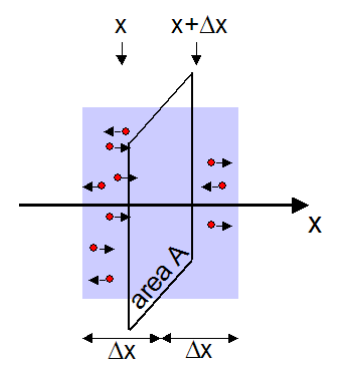
\includegraphics[scale=0.7]{Figures/ficks_diffusion_law.png}
    \caption{Τυχαία κίνηση σωματιδίων σε μία διάσταση, διερχόμενα από επιφάνεια $A$.}
    \label{fig:ficks_diffusion_law}
\end{figure}

Η διάδοση ενέργειας με ακτινοβολία μπορεί να προσεγγιστεί ως μια διαδικασία διάχυσης (diffusion) όπως θα δείξουμε. Έστω μοναδιαία επιφάνεια και σωματίδια (π.χ. φωτόνια) τα οποία διέρχονται διαμέσου αυτής της επιφάνειας κατά μία διεύθυνση $x$ (στην περίπτωσή μας αυτή η διεύθυνση θα ήταν η ακτινική και το $\Delta x = \ell$), όπως φαίνεται στο σχήμα \ref{fig:ficks_diffusion_law}. Αριστερά της επιφάνειας η αριθμητική πυκνότητα των σωματιδίων είναι $n(x)$ και δεξιά $n(x+\Delta x)$. Υποθέτοντας ότι οι ταχύτητες στις τρεις διευθύνσεις του χώρου είναι κατανεμημένες ισοτροπικά ώστε $u_x = u_y = u_z$, προκύπτει ότι για μία από τις τρεις διευθύνσεις, $u_x = \frac{1}{3} \langle u \rangle$. Το ερώτημα είναι πόσα σωματίδια διέρχονται από την επιφάνεια $A$. Διαστασιακά, η ροή των σωματιδίων μπορεί να γραφτεί ως $F = n \,u$, και επειδή τα σωματίδια έχουν την ίδια πιθανότητα να κινούνται είτε προς τα αριστερά είτε προς τα δεξιά, τα μισά σωματίδια θα κινούνται προς τη μία κατεύθυνση και τα άλλα μισά προς την άλλη. Έτσι, η ροή για τα σωματίδια που κινούνται διαμέσου της επιφάνειας $A$, από τα αριστερά προς τα δεξιά θα είναι
\begin{equation*}
    F(x) = \frac{1}{2} n(x) \,\frac{1}{3} \langle u \rangle = \frac{1}{6} n(x) \,\langle u \rangle
\end{equation*}
Αντίστοιχα, η ροή των σωματιδίων που κινούνται διαμέσου της επιφάνειας $A$, από τα δεξιά προς τα αριστερά θα είναι
\begin{equation*}
    F(x + \Delta x) = \frac{1}{6} n(x+\Delta x) \,\langle u \rangle
\end{equation*}
Έτσι, η θετική (net) ροή θα είναι
\begin{equation*}
    F = \frac{1}{6} \langle u \rangle \left[ n(x+\Delta x) - n(x) \right]
\end{equation*}
Επειδή οι αριθμοί $n(x), \,n(x + \Delta x)$ δεν είναι σταθεροί αλλά μεταβάλλονται ανάλογα με τον αριθμό των σωματιδίων που διαπερνούν την επιφάνεια και καταλήγουν είτε αριστερά είτε δεξιά, η τελευταία σχέση γράφεται
\begin{align}
    \nonumber F &= \frac{1}{6} \langle u \rangle \left[ n - \frac{dn}{dx}\Delta x - \left( n + \frac{dn}{dx}\Delta x \right) \right] = - \frac{1}{3} \langle u \rangle \Delta x \frac{dn}{dx} \Rightarrow \\ \nonumber \\
    &\Rightarrow F = -D \frac{dn}{dx}
\end{align}
όπου ο συντελεστής $D = \frac{1}{3} \langle u \rangle \Delta x$ ονομάζεται "διαχυσιμότητα" (diffusivity) και αποτελεί μέτρο του ρυθμού με τον οποίο τα σωματίδια διασκορπίζονται. Το παραπάνω αποτέλεσμα γενικεύεται στις τρεις διαστάσεις
\begin{equation}
    \label{eq:ficks_diffusion_law}
    F = - D \nabla n
\end{equation}
και είναι γνωστό ως \textbf{νόμος διάχυσης του Fick}.

Αντί της αριθμητικής πυκνότητας $n$, μπορούμε να γράψουμε κατά αντιστοιχία ότι η ροή ενέργειας λόγω διάχυσης είναι
\begin{equation}
    \label{eq:energy_density_diffusion}
    F = -D \nabla u \xrightarrow{1D} F = -D \frac{du}{dr}
\end{equation}
όπου $u$ η πυκνότητα ενέργειας. Χρησιμοποιοώντας τον κανόνα αλυσίδας $\frac{du}{dT} \,\frac{dT}{dr}$, μπορούμε να γράψουμε την σχέση \eqref{eq:energy_density_diffusion} ως
\begin{equation}
    \label{eq:temperature_gradient_diffusion_law}
    F = -D \underbrace{\frac{du}{dT}}_{= \,C_{\text{V}}} \,\frac{dT}{dr} = - K\frac{dT}{dr} \xrightarrow{3D} \boxed{F = -K \nabla T}
\end{equation}
όπου ο συντελεστής 
\begin{equation}
    \label{eq:conductivity_diffusion_coefficient}
    K = \frac{1}{3} \langle u \rangle \ell C_{\text{V}} = \frac{1}{3 \kappa_\nu \rho} \langle u \rangle C_{\text{V}}
\end{equation}
ονομάζεται "αγωγιμότητα" (conductivity) και 
\begin{equation}
    \label{eq:specific_heat_capacity}
    C_{\text{V}} = \left( \frac{du}{dT} \right)_{\text{V}}
\end{equation}
η ειδική θερμοχωρητικότητα (specific heat capacity). Αυτή η περιγραφή ισχύει για όλα τα σωματίδια σε τοπική θερμοδυναμική ισορροπία, συμπεριλαμβανομένων και των φωτονίων. 

Για ένα αέριο φωτονίων, μπορούμε να θέσουμε $\langle u \rangle = c$, όπου $c$ η ταχύτητα του φωτός στο κενό. Η πυκνότητα ενέργειας δίνεται από τη σχέση \eqref{eq:photon_energy_density} και άρα η ειδική θερμοχωρητικότητα είναι
\begin{equation*}
    C_{\text{V}} = \left( \frac{du}{dT} \right)_{\text{V}} = 4 \alpha T^3
\end{equation*}
ενώ η μέση ελεύθερη διαδρομή σχετίζεται με την αδιαφάνεια μέσω της σχέσης \eqref{eq:mean_free_path}, όπου αν πάρουμε την μέση τιμή για όλες τις συχνότητες ($\langle \kappa \rangle \equiv \kappa$) μπορεί να γραφτεί
\begin{equation*}
    \ell_{\text{ph}} = \frac{1}{\kappa \rho}
\end{equation*}
Συνδυάζοντας όλα τα παραπάνω, μπορούμε να γράψουμε τον \textbf{συντελεστή αγωγιμότητας ακτινοβολίας} \eqref{eq:conductivity_diffusion_coefficient} ως
\begin{equation}
    \label{eq:radiation_conductivity_coefficient}
    K_{\text{rad}} = \frac{4}{3} \frac{\alpha \,c \,T^3}{\kappa \rho}
\end{equation}

Σε αυτό το σημείο αξίζει να αναφέρουμε ότι και η διάδοση ενέργειας μέσω αγωγής μπορεί να περιγραφεί ως μία διαδικασία διάχυσης με την ίδια συναρτησιακή μορφή της σχέσης \eqref{eq:temperature_gradient_diffusion_law} ώστε η συνδυαστική ροή ενέργειας να είναι
\begin{equation}
    \label{eq:radiative_and_conduction_flux}
    F = - \frac{4\alpha c T^3}{3\rho}\left( \frac{1}{\kappa_{\text{rad}}} + \frac{1}{\kappa_{\text{cd}}} \right) \nabla T
\end{equation}
όπου ορίσαμε την \textbf{αδιαφάνεια αγωγής}, $\kappa_{\text{cd}}$, σε αναλογία με την αδιαφάνεια ακτινοβολίας $\kappa_{\text{rad}}$. Αυτό το αποτέλεσμα σημαίνει απλά ότι ο μηχανισμός διάδοσης ενέργειας με τη μεγαλύτερη ροή θα είναι ο κυριάρχος, ή με άλλα λόγια, ο μηχανισμός για τον οποίο η αστρική ύλη παρουσιάζει τη μεγαλύτερη διαφάνεια.

Για έναν σφαιρικά συμμετρικό αστέρα, η τοπική λαμπρότητα σχετίζεται με την ροή μέσω της σχέσης 
$$F = \frac{l}{4\pi r^2}$$
και άρα η εξίσωση \eqref{eq:radiative_and_conduction_flux} γράφεται
\begin{align}
    \label{eq:energy_transport_radiation_eulerian_diff}
    \nonumber F_{\text{rad}} &= - \frac{4}{3} \frac{\alpha \,c \,T^3}{\kappa_{\text{rad}} \rho} \frac{dT}{dr} = \frac{l}{4\pi r^2} \Rightarrow \\ \nonumber \\
    &\Rightarrow \boxed{\frac{dT}{dr} = - \frac{3\kappa \rho}{16 \pi \alpha c T^3} \frac{l}{r^2}}
\end{align}
ή στο σύστημα συντεταγμένων του Lagrange
\begin{equation}
    \label{eq:energy_transport_radiation_lagrangian_diff}
    \boxed{\frac{dT}{dm} = - \frac{3}{64\pi^2 \alpha c} \frac{\kappa l}{r^4 T^3}}
\end{equation}
Αυτή είναι η θερμοβαθμίδα που απαιτείται ώστε όλη η λαμπρότητα $l$ να μεταφερθεί μέσω ακτινοβολίας και αποτελεί την τέταρτη διαφορική εξίσωση που περιγράφει τη δομή ενός αστέρα στην περίπτωση που έχουμε διάδοση ενέργειας μόνο μέσω ακτινοβολίας. Ένα αστέρι ή μια περιοχή ενός αστεριού στην οποία ισχύει αυτή η εξίσωση ονομάζεται ζώνη ακτινοβολίας (radiative).

Η εξίσωση \eqref{eq:energy_transport_radiation_lagrangian_diff} ισχύει όσο $\ell_{\text{ph}} \ll R$, δηλαδή όσο υπάρχει τοπική θερμοδυναμική ισορροπία. Αυτή η συνθήκη σταματάει να ισχύει όσο πλησιάζουμε την επιφάνεια του αστέρα, την φωτόσφαιρα, από την οποία διαφεύγουν φωτόνια ($\ell_{\text{ph}} \gtrsim R$). Κοντά στην φωτόσφαιρα, η προσέγγιση της διάχυσης παύει να ισχύει και πρέπει να λύσουμε την --πολύ πιο δύσκολη-- εξίσωση μεταφοράς. Ευτυχώς, συνθήκες τοπικής θερμοδυναμικής ισορροπίας και η προσέγγιση της διάχυσης ισχύουν σχεδόν για όλο το εσωτερικό των αστέρων.

Για έναν αστέρα που βρίσκεται σε υδροστατική ισορροπία, μπορούμε συνδυάζοντας τις εξισώσεις \eqref{eq:hydrostatic_equilibrium_lagrangian_coordinate} και \eqref{eq:energy_transport_radiation_lagrangian_diff} να γράψουμε την θερμοβαθμίδα ως
\begin{equation*}
    \frac{dT}{dm} = \frac{dP}{dm} \,\frac{dT}{dP} = - \frac{Gm}{4\pi r^4} \,\frac{T}{P} \,\frac{d\log T}{d\log P}
\end{equation*}
ώστε να ορίσουμε την αδιάστατη θερμοβαθμίδα ακτινοβολίας (radiative temperature gradient)
\begin{eqnarray}
    \label{eq:radiative_temperature_gradient}
    \nabla_{\text{rad}} = \left(\frac{d\log T}{d\log P} \right)_{\text{rad}} = \frac{3}{16\pi \alpha c G} \frac{\kappa l P}{m T^4}
\end{eqnarray}
Η σχέση \eqref{eq:radiative_temperature_gradient} περιγράφει την λογαριθμική μεταβολή της θερμοκρασίας με το βάθος (όπου το βάθος είναι εκφρασμένο μέσω της πίεσης) σε έναν αστέρα σε υδροστατική ισορροπία, αν η ενέργεια μεταφέρεται μόνο μέσω ακτινοβολίας.
%% ---------------------------------------------------------------------------------------------------- %%
%% ---------------------------------------------------------------------------------------------------- %%
%% ---------------------------------------------------------------------------------------------------- %%
\subsubsection{Η αδιαφάνεια στο εσωτερικό των αστέρων}
Οι εξισώσεις που περιγράφουν την διάχυση της ακτινοβολίας είναι ανεξάρτητες της συχνότητας $\nu$, αφού η ροή $F$ ολοκληρώνεται ως προς όλες τις συχνότητες. Γενικά όμως, ο συντελεστής αδιαφάνειας $\kappa_\nu$ εξαρτάται από την συχνότητα, οπότε η ποσότητα $\kappa$ που εμφανίζεται στην σχέση \eqref{eq:energy_transport_radiation_lagrangian_diff}
πρέπει να παριστάνει έναν μέσο όρο ως προς τη συχνότητα.

Αν με $F_\nu d\nu$ θεωρήσουμε την ροή ακτινοβολίας στο διάστημα συχνοτήτων $[\nu, \nu+d\nu]$, τότε η εξίσωση \eqref{eq:ficks_diffusion_law} πρέπει να αντικατασταθεί με
\begin{equation}
    \label{eq:ficks_diffusion_law_frequency_dependent}
    F_\nu = -D_\nu \nabla u_\nu = -D_\nu \frac{\partial u_\nu}{\partial T} \nabla T
\end{equation}
όπου $D_\nu = \frac{1}{3} c l_{\text{ph}} = \frac{c}{3 \kappa_nu \rho}$.  Επειδή θεωρούμε ότι η ακτινοβολία βρίσκεται σε θερμική ισορροπία με το αέριο, η πυκνότητα ενέργειας στο ίδιο διάστημα, συνδέεται με την ένταση της ακτινοβολίας που δίνεται από τον νόμο του Planck μεσω της σχέσης
\begin{equation}
    \label{eq:energy_density_intensity_correlation}
    B_\nu (T) = \frac{u_\nu (T) \,c}{4\pi}
\end{equation}
Η ολική ροή προκύπτει από την ολοκλήρωση της σχέσης \eqref{eq:ficks_diffusion_law_frequency_dependent} σε όλες τις συχνότητες
\begin{equation*}
    F = - \left[\frac{c}{3 \rho} \int_{0}^{\infty} \frac{1}{\kappa_\nu} \frac{\partial u_{\nu}}{\partial T} d\nu \right] \nabla T
\end{equation*}
η οποία έχει την ίδια μορφή με τη σχέση \eqref{eq:temperature_gradient_diffusion_law} όπου 
\begin{equation*}
    K_{\text{rad}} = \frac{c}{3 \rho} \int_{0}^{\infty} \frac{1}{\kappa_\nu} \frac{\partial u_{\nu}}{\partial T} d\nu
\end{equation*}
Συγκρίνοντας το παραπάνω αποτέλεσμα με τη σχέση \eqref{eq:radiation_conductivity_coefficient} καταλήγουμε ότι
\begin{equation}
    \frac{1}{\kappa} = \frac{1}{4\alpha T^3} \int_{0}^{\infty} \frac{1}{\kappa_\nu} \frac{\partial u_{\nu}}{\partial T} d\nu
\end{equation}
όπου ο παράγοντας $4 \alpha T^3$ ισούται με $\int_{0}^{\infty} \frac{\partial u_\nu}{\partial T} d\nu$ ώστε η παραπάνω σχέση να γράφεται γενικά
\begin{equation}
    \label{eq:rosseland_mean_opacity_energy_density}
    \frac{1}{\kappa} = \frac{\int_{0}^{\infty} \frac{1}{\kappa_\nu} \frac{\partial u_{\nu}}{\partial T} d\nu}{\int_{0}^{\infty} \frac{\partial u_\nu}{\partial T} d\nu}
\end{equation}
Η ποσότητα $\kappa$ ονομάζεται \textbf{μέση αδιαφάνεια κατά Rosseland} και είναι η αρμονική μέση τιμή της αδιαφάνεια ενός αερίου συγκεκριμένης σύστασης, θερμοκρασίας και πυκνότητας, ως προς όλες τις συχνότητες της ακτινοβολίας που απορροφάται ή σκεδάζεται (σταθμισμένη με στατιστικό βάρος τη συνάρτηση $\partial u_\nu / \partial T$). Συχνά η μέση αδιαφάνεια κατά Rosseland εμφανίζεται με τον όρο της έντασης της ακτινοβολίας αντί της πυκνότητας ενέργειας, ώστε χρησιμοποιώντας την σχέση \eqref{eq:energy_density_intensity_correlation} να γράφεται και
\begin{equation*}
    \frac{1}{\kappa} = \frac{\pi}{\alpha c T^3} \int_{0}^{\infty} \frac{1}{\kappa_\nu} \frac{\partial B_{\nu} (T)}{\partial T} d\nu
\end{equation*}
ή γενικά

\begin{equation}
    \label{eq:rosseland_mean_opacity_intensity}
    \boxed{\frac{1}{\kappa} \int_{0}^{\infty} \frac{\partial B_{\nu} (T)}{\partial T} d\nu = \int_{0}^{\infty} \frac{1}{\kappa_\nu} \frac{\partial B_{\nu} (T)}{\partial T} d\nu}
\end{equation}

Όταν μελετάμε το εσωτερικό των αστέρων, δεν ενδιαφερόμαστε ιδιαίτερα για την ειδική ένταση $I_\nu$ (και την αντίστοιχη λαμπρότητα $L_\nu$), αφού δεν είναι δυνατόν να παρατηρήσουμε την κατανομή της λαμπρότητας με τη συχνότητα. Αντίθετα, ενδιαφερόμαστε για την ολική λαμπρότητα, $L$, η οποία συνδέεται άμεσα με το ενεργειακό ισοζύγιο του αστέρα (αφού σε κατάσταση ισορροπίας, η ενέργεια που ακτινοβολείται ως λαμπρότητα αναπληρώνεται από τις πηγές ενέργειας του αστέρα). Η μέση αδιαφάνεια κατά Rosseland είναι χρήσιμη όταν θέλουμε να υπολογίσουμε τη συνολική ενέργεια που απορροφήθηκε σε όλα τα μήκη κύματος, κάτι που απαιτείται στους υπολογισμούς της αστρικής δομής.


Ο συντελεστής αδιαφάνειας στο εσωτερικό των αστέρων οφείλεται στους μηχανισμούς που περιγράψαμε στο Κεφάλαιο \ref{ch:Chapter4}, δηλαδή σε φωτοϊονισμό (bound-free transition), σε πέδηση (free-free transition) ή σε σκεδάσεις (Thomson και Compton). Ο συντελεστής αδιαφάνειας που οφείλεται σε σκεδάσεις φωτονίων από ηλεκτρόνια, $\kappa_{\text{scat}}$, αποδεικνύεται ότι εξαρτάται μόνο από τη χημική σύσταστη της ύλης του αστέρα, και δίνεται από τη σχέση
\begin{equation}
    \label{eq:opacity_scattering}
    \kappa_{\text{scat}} = 0.2 (1+X) \,\text{cm$^2$/gr}
\end{equation}
όπου $X$ είναι η περιεκτικότητα της ύλης σε υδρογόνο. Παρατηρούμε ότι ο συντελεστής απορρόφησης λόγω σκέδασης από ηλεκτρόνια είναι ανεξάρτητος από τη συχνότητα των φωτονίων.

Οι συντελεστές απορρόφησης των δύο άλλων μηχανισμών, $\kappa_{\nu}^{\text{bf}}$ και $\kappa_{\nu}^{\text{ff}}$, είναι συναρτήσεις \textit{και} της συχνότητας, και επομένως χρειαζόμαστε τις αντίστοιχες αδιαφάνειες κατά Rosseland, $\kappa_{\text{bf}}$ και $\kappa_{\text{ff}}$. Αυτές έχουν υπολογιστεί από τον Kramer και δίνονται από τις σχέσεις
\begin{align}
    \kappa_{\text{bf}} &= a(X,Z,g_a,t) \rho T^s \label{eq:opacity_bound_free} \\ \nonumber \\
    \kappa_{\text{ff}} &= b(X,Z,g_b) \rho T^s \label{eq:opacity_free_free}
\end{align}
όπου ο εκθέτης, $s$, είναι συνάρτηση της θεμοκρασίας. Για τις υψηλές θερμοκρασίες που επικρατούν στο εσωτερικό των αστέρων ($T \geq 10^5$) αποδεικνύεται ότι $s = -3.5$, ενώ για σχετικά χαμηλές θερμοκρασίες ($T \approx 10^4$) αποδεικνύεται ότι $s = 10$. Οι συναρτήσεις $a, b$, στην περίπτωση που $s=-3.5$, ορίζονται από τις σχέσεις
\begin{align}
    a &= 4.34 \times 10^{25} \,\frac{g_a}{t} Z(1 + X) \label{eq:gaunt_factor_bf} \\ \nonumber \\
    b &= 3.68 \times 10^{22} \,g_b (1 + X) (1 - Z) \label{eq:gaunt_factor_ff}
\end{align}
Στις παραπάνω σχέσεις, οι συντελεστές $g_a, g_b$ και $t$ ονομάζονται \textbf{συντελεστές Gaunt} και \textbf{συντελεστής αποκοπής} (guillotine factor) αντίστοιχα. Οι συντελεστές Gaunt διορθώνουν τις αποκλίσεις μεταξύ της κλασικής και κβαντομηχανικής λύσης, ενώ ο συντελεστής αποκοπής διορθώνει τα σφάλματα των προσεγγίσεων κατά τον υπολογισμό της σχέσης \eqref{eq:gaunt_factor_bf}. Συνηθισμένες τιμές για τους συντελεστές αυτούς είναι $g_a \approx g_b \approx 3$ και $t \approx 10$. Το $X$ αντιπροσωπεύει την περιεκτικότητα (κατά μάζα) της ύλης του αστέρα σε υδρογόνο και το $Z$ την περιεκτικότητα της ύλης του αστέρα σε στοιχεία βαρύτερα από το ήλιο ("μέταλλα"), γι΄ αυτό και ονομάζεται και "metallicity".

Είθισται, οποιαδήποτε σχέση για την αδιαφάνεια έχει τη μορφή
\begin{equation}
    \label{eq:kramers_opacity_law_form}
    \kappa \propto \rho T^{-7/2}
\end{equation}
να ονομάζεται \textbf{αδιαφάνεια κατά Kramer}.

Από τους ορισμούς των $\kappa_{\text{bf}}, \kappa_{\text{ff}}$ παρατηρούμε ότι η αδιαφάνεια κατά Kramer είναι φθίνουσα συνάρτητη της θερμοκρασίας. Έτσι, σε αρκετά μεγάλες θερμοκρασίες ($T > 10^8 \,\text{K}$) η τιμή της τείνει στο μηδέν και επομένως γίνεται μικρότερη από την αδιαφάνεια σκέδασης απο ηλεκτρόνια $\kappa_{\text{scat}}$ (που είναι ανεξάρτητη της θερμοκρασίας). Από το αποτέλεσμα αυτό συμπεραίνουμε ότι η αδιαφάνεια κατά Kramer (μηχανισμοί bound-free και free-free) κυριαρχεί στους (ψυχρότερους) αστέρες μεταγενέστερων φασματικών τύπων, ενώ η αδιαφάνεια σκέδασης από ηλεκτρόνια κυριαρχεί στους (θερμότερους) αστέρες των προγενέστερων φασματικών τύπων.
%% ---------------------------------------------------------------------------------------------------- %%
%% ---------------------------------------------------------------------------------------------------- %%
%% ---------------------------------------------------------------------------------------------------- %%
\subsubsection{Το όριο Eddington}
Είδαμε ότι η διάδοση ενέργειας μέσω ακτινοβολίας μέσα σε έναν αστέρα απαιτεί μία θερμοβαθμίδα $dT/dr$, το μέγεθος της οποίας δίνεται από την εξίσωση \eqref{eq:energy_transport_radiation_eulerian_diff}. Η πίεση της ακτινοβολίας δίνεται από τη σχέση \eqref{eq:radiation_pressure_black_body} και άρα η βαθμίδα της πίεσης της ακτινοβολίας είναι
\begin{equation}
    \label{eq:radiation_pressure_gradient}
    \frac{dP_{\text{rad}}}{dr} = \frac{4}{3} \alpha T^3 \,\frac{dT}{dr} = - \frac{\kappa \rho}{4\pi c} \frac{l}{r^2}
\end{equation}
Αυτή η πίεση της ακτινοβολίας παριστάνει μία δύναμη που ασκείται προς το εξωτερικό του αστέρα λόγω της ροής των φωτονίων προς αυτή την κατεύθυνση. Φυσικά, για έναν αστέρα που βρίσκεται σε υδροστατική ισορροπία, αυτή η δύναμη πρέπει να είναι μικρότερη από τη δύναμη της βαρύτητας, όπως αυτή δίνεται από τη βαθμίδα της πίεσης που είναι απαραίτητη για την εδραίωση της υδροστατικής ισορροπίας (σχέση \ref{eq:hydrostatic_equilibrium_eulerian coordinates}). Αυτό σημαίνει ότι
\begin{align}
    \label{eq:eddington_limit}
    \nonumber \left| \frac{dP_{\text{rad}}}{dr} \right| &< \left| \left( \frac{dP}{dr} \right)_{\text{HE}} \right| \Rightarrow \frac{\kappa \rho}{4 \pi c} \frac{l}{r^2} < \frac{G m \rho}{r^2} \\ \nonumber \\
    &\Rightarrow l < \frac{4\pi G m c}{\kappa} = l_{\text{Edd}}
\end{align}
Η ποσότητα $l_{\text{Edd}} = \frac{4\pi G m c}{\kappa}$ ονομάζεται (τοπική) \textbf{λαμπρότητα Eddington} και παριστάνει τη μέγιστη λαμπρότητα που μπορεί να μεταφερθεί από την ακτινοβολία σε έναν αστέρα που βρίσκεται σε υδροστατική ισορροπία.

Το όριο Eddington που παριστάνεται από την ανισότητα \eqref{eq:eddington_limit} μπορεί να παραβιαστεί σε περιπτώσεις πολύ μεγάλων ροών θερμότητας (μεγάλα $l$), οι οποίες προκαλούνται από έντονη "καύση" των πυρηνικών καυσίμων, ή από πολύ μεγάλες αδιαφάνειες $\kappa$. Όπως αναφέραμε παραπάνω, υψηλές τιμές αδιαφάνειας εμφανίζονται σε σχετικά χαμηλές θερμοκρασίες, κοντά στην θερμοκρασία ιονισμού του υδρογόνου και του ηλίου (π.χ. εξωτερικά στρώματα του Ήλιου). Σε αυτές τις περιπτώσεις, η υδροστατική ισορροπία (σχέση \ref{eq:hydrostatic_equilibrium_eulerian coordinates}) και η ισορροπία λόγω της μεταφοράς ενέργειας με ακτινοβολία (radiative equilibrium, σχέση \ref{eq:energy_transport_radiation_eulerian_diff}) δεν μπορούν να ισχύουν ταυτόχρονα. Γι' αυτό, προκειμένου ο αστέρας να παραμείνει σε υδροστατική ισορροπία, η ενέργεια πρέπει να μεταφερθεί με άλλον τρόπο εκτός της διάχυσης ακτινοβολίας. Αυτός ο τρόπος είναι μέσω ρευμάτων μεταφοράς που θα αναλύσουμε παρακάτω. Ισχύει ότι η ανισότητα \eqref{eq:eddington_limit} είναι αναγκαία, αλλά όχι ικανή συνθήκη για μία ζώνη ενός αστέρα να είναι σταθερή ενάντια στα ρεύματα μεταφοράς.

Τα επιφανειακά στρώματα ενός αστέρα διαδίδουν πάντα την ενέργεια μέσω ακτινοβολίας αφού είναι εκείνη η περιοχή από την οποία η ενέργεια διαφεύγει με τη μορφή φωτονίων. Εφαρμόζοντας τη σχέση \eqref{eq:eddington_limit} στην επιφάνεια του αστέρα όπου $m=M$ προκύπτει
\begin{equation}
    \label{eq:eddington_surface_limit}
    L < L_{\text{Edd}} = \frac{4\pi G M c}{\kappa} 
\end{equation}
όπου $\kappa$ είναι η αδιαφάνεια της φωτόσφαιρας. Η λαμπρότητα Eddington που δίνεται από την σχέση \eqref{eq:eddington_surface_limit} είναι μία κριτική τιμή λαμπρότητας που δεν μπορεί να ξεπεραστεί από έναν αστέρα σε υδροστατική ισορροπία. Παραβίαση αυτής της συνθήκης σημαίνει παραβίαση της υδροστατικής ισορροπίας: η ύλη εκδιώχνεται από τον αστέρα λόγω της πίεσης της ακτινοβολίας, οδηγώντας σε βίαιη απώλεια μάζας. Όπως είδαμε και παραπάνω, σε περιοχές που κυριαρχεί η σκέδαση φωτονίων από ηλεκτρόνια, η αδιαφάνεια είναι σχεδόν σταθερή και άρα η λαμπρότητα Eddington εξαρτάται μόνο από τη μάζα
\begin{equation}
    \label{eq:eddington_luminosity_electron_scattering_opacity}
    L_{\text{Edd}} = \frac{4\pi G M c}{0.2 (1+X)} = \frac{2.52 \times 10^{38}}{1+X} \left( \frac{M}{M_\odot} \right) \,\text{erg/s}
\end{equation}

Επειδή η $L_{\text{Edd}}$ είναι ανάλογη της μάζας $m$, ενώ οι αστέρες της κύριας ακολουθίας ακολουθούν μία σχέση λαμπρότητας-μάζας (Κεφάλαιο \ref{ch:Chapter2}) $L \propto M^x,  \,x>1$, αυτό σημαίνει ότι όσο αυξάνεται η μάζα των αστέρων κάποια στιγμή η λαμπρότητά τους θα ξεπεράσει το όριο Eddington. Άρα, περιμένουμε να υπάρχει κάποιο ανώτερο όριο στη μάζα που μπορούν να έχουν οι αστέρες, το οποίο βρίσκεται με απαλοιφή της λαμπρότητας από τις δύο παραπάνω σχέσεις.

Υιοθετώντας μία σχέση λαμπρότητας-μάζας
\begin{equation}
    \label{eq:observed_mass_luminosity_relation}
    \frac{L}{L_\odot} = 3.013 \left( \frac{M}{M_\odot} \right)^{2.91}
\end{equation}
από τις σχέσεις \eqref{eq:eddington_luminosity_electron_scattering_opacity} και \eqref{eq:observed_mass_luminosity_relation} προκύπτει ότι
\begin{align*}
    11.54 &\times 10^{33} \left( \frac{M}{M_\odot} \right)^{2.91} = \frac{2.52 \times 10^{38}}{1+X} \left( \frac{M}{M_\odot} \right) \Rightarrow \\\\
    &\Rightarrow \left( \frac{M}{M_\odot} \right)^{1.91} = \frac{2.16 \times 10^4}{1+X} \Rightarrow \\\\
    &\Rightarrow M_{\text{max}} = \left(\frac{2.16 \times 10^4}{1+X} \right)^{0.524} \,M_\odot
\end{align*}
Για μία χημική σύσταση με 70\,\% υδρογόνο ($X=1$), έχουμε ότι
\begin{equation}
    M_{\text{max}} \simeq 140 \,M_{\odot}
\end{equation}
τιμή η οποία είναι συμβατή με τις μέχρι τώρα παρατηρήσεις καθώς δεν έχουμε εντοπίσει αστέρες με μάζα μεγαλύτερη των $100 \,M_\odot$.
%% ---------------------------------------------------------------------------------------------------- %%
%% ---------------------------------------------------------------------------------------------------- %%
%% ---------------------------------------------------------------------------------------------------- %%
\subsubsection{Σχέσεις λαμπρότητας-μάζας}
Είδαμε ότι τα φωτόνια που εκπέμπονται από τις πυρηνικές αντιδράσεις που λαμβάνουν χώρα στον πυρήνα ενός αστέρα, απορροφούνται σχεδόν αμέσως και επανεκπέμπονται σε μεγαλύτερα μήκη κύματος\footnote{ Η διαφορά ενέργειας μεταξύ του φωτονίου που απορροφήθηκε και αυτού που εκπέμφθηκε πήγε στην θέρμανση του υλικού.} από ανώτερα στρώματα προς τυχαίες διευθύνσεις, μία διαδικασία που ονομάζεται "\textbf{τυχαίος βηματισμός}" (random walk) και μπορεί να θεωρηθεί ως μια διαδικασία διάχυσης της ακτινοβολίας. Από τη θεωρία του τυχαίου βηματισμού γνωρίζουμε ότι τα βήματα που απαιτούνται για να καλύψει ένα φωτόνιο μία μέση απόσταση ίση με την ακτίνα του αστέρα είναι
\begin{equation}
    \label{eq:random_walk_steps}
    N = \left( \frac{R}{\ell_{\text{ph}}} \right)^2
\end{equation}
Αυτό συνεπάγεται ότι ο μέσος χρόνος που χρειάζονται τα φωτόνια για να διανύσουν απόσταση $\ell_{\text{ph}}$ λόγω διάχυσης είναι
\begin{equation}
    \label{eq:diffusion_time}
    t_{\text{diffusion}} = \frac{\ell_{\text{ph}}}{c} N = \frac{R^2}{\ell_{\text{ph}} c}
\end{equation}

Έστω τώρα ότι η ακτίνα του πυρήνα ενός αστέρα είναι κάποιο κλάσμα της συνολικής ακτίνας του αστέρα $R_c = fR, \,f<1$. Η πυκνότητα ενέργειας που παράγεται στον πυρήνα είναι $u=\alpha T_c^4$ και άρα η συνολική διαθέσιμη ενέργεια του πυρήνα είναι 
\begin{equation}
    E = \frac{4}{3} \pi R_c^3 \,\alpha T_c^4
\end{equation}

Σε πρώτη προσέγγιση, η μέση λαμπρότητα θα είναι τότε
\begin{equation}
    L \approx \frac{E_c}{t_{\text{diffusion}}} = \frac{\frac{4\pi}{3} (fR)^3 \alpha T_c^4}{\left( \frac{R^2}{\ell_{\text{ph}} c} \right)} \Rightarrow \boxed{ L \propto R \ell_{\text{ph}} T_c^4}
\end{equation}

Για να βρούμε μία σχέση $L = f(M)$, πρέπει να βρούμε σχέσεις που να συνδέεουν τις ποσότητες $R, \ell_{\text{ph}}, T_c$ με τη μάζα. Από τις σχέσεις \eqref{eq:mean_free_path}, \eqref{eq:lower_limit_of_central_pressure_for_stars_in_HE} έχουμε ότι
\begin{align*}
    \ell_{\text{ph}} &\propto \frac{1}{\langle \rho \rangle} \\\\
    \langle \rho \rangle &\propto \frac{M}{R^3} \\\\
    P_c &\propto \frac{M^2}{R^4}
\end{align*}

Έτσι, μπορούμε να διακρίνουμε τις εξής περιπτώσεις
\begin{itemize}
    \item Για αστέρες μεγάλης μάζας, $M>30M_\odot$, ο κυρίαρχος μηχανισμός πίεσης είναι η πίεση ακτινοβολίας $P_{\text{rad}} = \frac{1}{3} \alpha T_c^4$ και άρα
    \begin{equation*}
        P_c \propto \frac{M^2}{R^4} \propto T_c^4
    \end{equation*}
    Συνεπώς
    \begin{equation}
        \label{eq:high_mass_LM_relationship}
        L \propto R \frac{1}{\langle \rho \rangle} T_c^4 \Rightarrow \boxed{L \propto M}
    \end{equation}
    
    \item Για αστέρες ενδιάμεσης μάζας, $3M_\odot < M < 30M_\odot$, ισχύουν οι ίδιες σχέσεις με παραπάνω αλλά τώρα ο κυρίαρχος μηχανισμός πίεσης είναι η πίεση του αερίου $P_{\text{gas}} \propto \rho T_c$ και άρα
    \begin{equation*}
        P_c \propto \frac{M^2}{R^4} \propto \rho T_c \longrightarrow T_c \propto \frac{M^2}{R^4} \frac{1}{\langle \rho \rangle}
    \end{equation*}
    Συνεπώς
    \begin{equation}
        \label{eq:intermediate_mass_LM_relationship}
        L \propto R \frac{1}{\langle \rho \rangle} \left(\frac{M^2}{R^4} \frac{1}{\langle \rho \rangle} \right)^4 \Rightarrow \boxed{L \propto M^3}
    \end{equation}
\end{itemize}
%% ---------------------------------------------------------------------------------------------------- %%
%% ---------------------------------------------------------------------------------------------------- %%
%% ---------------------------------------------------------------------------------------------------- %%
\subsubsection{Διάδοση ακτινοβολίας με ρεύματα μεταφοράς}
Στην Αστροφυσική συχνά συναντάμε προβλήματα όπου ένα ρευστό θερμαίνεται από "κάτω" (π.χ. αστέρες, ατμόσφαιρα της Γης όπου ο Ήλιος θερμαίνει την επιφάνεια κτλ). Αυτό οδηγεί σε μια θερμοβαθμίδα: ζεστό στη βάση, πιο ψυχρό προς τα πάνω\footnote{Εδώ ο όρος "πάνω" θα αναφέρεται στην αντίθετη κατεύθυνση από αυτή της βαρύτητας.}. Αν η θερμοβαθμίδα γίνει πολύ μεγάλη, το αέριο αναπτύσσει ένα είδος αστάθειας (convective instability) ώστε "φυσαλίδες" αερίου που είναι πιο θερμές από το περιβάλλον στο οποίο βρίσκονται, μετακινούνται προς τα ανώτερα στρώματα μέχρι να διασκορπίσουν (dissipate) την περίσσεια θερμική ενέργεια που κουβαλούν και να ενσωματωθούν στο καινούργιο περιβάλλον, υιοθετώντας όλες τις ιδιότητες που το χαρακτηρίζουν (πίεση, θερμοκρασία κτλ). 

Έστω ένα στοιχειώδες κομμάτι αερίου με πυκνότητα $\rho_b$ και πίεση $P_b$ το οποίο βρίσκεται μέσα σε υλικό πυκνότητας $\rho$ και πίεσης $P$. Ας υποθέσουμε ότι λόγω κάποιων μικρών διαταραχών, το στοιχειώδες αυτό κομμάτι αερίου μετατοπίζεται προς τα επάνω κατά μία μικρή απόσταση $\delta z \equiv \delta r$. Μετά την μετατόπιση, το κομμάτι αερίου θα έχει συνθήκες ($\rho_b^{\star}, P_b^{\star}$) ενώ το καινούργιο του περιβάλλον θα χαρακτηρίζεται από συνθήκες ($\rho^{\prime}, P^{\prime}$), όπου
\begin{align}
    \rho^{\prime} &= \rho + \frac{d\rho}{dr} \delta r \label{eq:convection:density_perturbation} \\ \nonumber \\
    P^{\prime} &= P + \frac{dP}{dr} \delta r \label{eq:convection:pressure_perturbation}
\end{align}


\begin{figure}[t]
    \centering
    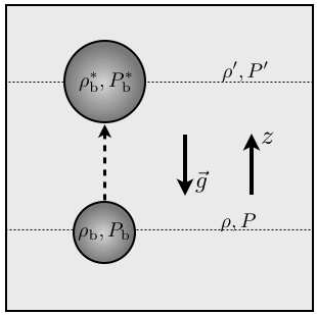
\includegraphics[scale=0.6]{Figures/convection_scheme.png}
    \caption{Σχηματική αναπαράσταση του κριτηρίου Schwarzschild ενάντια στην ύπαρξη ρευμάτων μεταφοράς. Ένα στοιχειώδες κομμάτι αερίου (blob) μετατοπίζεται προς την επιφάνεια του αστέρα όπου διαστέλλεται αδιαβατικά για να διατηρήσει μηχανική ισορροπία με το περιβάλλον του. Αν η πυκνότητα του στοιχειώδους κομματιού είναι μεγαλύτερη από την πυκνότητα του υλικού που το περιβάλλει, θα βυθιστεί πίσω στην αρχική του θέση. Αν όμως η πυκνότητά του είναι μικρότερη από την πυκνότητα του χώρου γύρω του, δυνάμεις άνωσης θα το επιταχύνουν προς τα επάνω και θα δημιουργηθεί ένα ρεύμα μεταφοράς.}
    \label{fig:convection_scheme}
\end{figure}

Αρχικά, το στοιχειώδες κομμάτι αερίου υποθέτουμε ότι βρισκόταν σε κατάσταση μηχανικής και θερμικής ισορροπίας με τον περιβάλλοντα χώρο, ώστε $\rho_b = \rho$ και $P_b = P$. Μετά την μετατόπιση, το κομμάτι πρέπει να επανέλθει σε μία νέα κατάσταση μηχανικής και θερμικής ισορροπίας. Γενικά, ο χρόνος που χρειάζεται για να εδραιώσει μία νέα κατάσταση μηχανικής ισορροπίας είναι ο δυναμικός χρόνος, $\tau_{\text{dyn}}$, ενώ η θερμική ισορροπία επέρχεται πολύ πιο αργά, στον θερμικό χρόνο $\tau_{\text{KH}}$. Επειδή ισχύει ότι $\tau_{\text{dyn}} \ll \tau_{\text{KH}}$, μπορούμε να υποθέσουμε ότι η μηχανική ισορροπία επέρχεται πριν προλάβει να γίνει ανταλλαγή θερμότητας με το περιβάλλον, ώστε η διαδικασία της μετατόπισης να είναι προσεγγιστικά αδιαβατική και να ισχύει $P_b^{\star} = P^{\prime}$ αλλά γενικά $\rho_b^{\star} \neq \rho^{\prime}$. Αυτό σημαίνει ότι η παραπάνω διαδικασία μπορεί να περιγραφεί από μία αδιαβατική καταστατική εξίσωση της μορφής $P \propto \rho^{\gamma}$, όπου $\gamma$ ο αδιαβατικός δείκτης. Έτσι, μπορούμε να γράψουμε

\begin{align*}
    \begin{cases}
        P_b &\propto \rho_b^{\gamma} \\
        P_b^{\star} &\propto {\rho_b^{\star}}^{\gamma}
    \end{cases} &\Rightarrow
    \frac{ P_b^{\star}}{P_b} \propto \left(\frac{\rho_b^{\star}}{\rho_b}\right)^{\gamma} \Rightarrow \rho_b^{\star} \propto \rho_b \left(\frac{P_b^{\star}}{P_b} \right)^{1/\gamma} \Rightarrow \\\\
    &\Rightarrow \rho_b^{\star} \propto \rho_b \left(\frac{P^{\prime}}{P} \right)^{1/\gamma} \xRightarrow{\eqref{eq:convection:pressure_perturbation}}{\rho_b^{\star} = \rho_b \left(1 + \frac{1}{P} \frac{dP}{dr}\delta r \right)^{1/\gamma}}
\end{align*}

Στο όριο των μικρών μετατοπίσεων $\delta r$, μπορούμε να χρησιμοποιήσουμε ανάπτυγμα Taylor για να δείξουμε ότι
\begin{eqnarray}
    \label{eq:convection:new_blob_density_expression}
    \rho_b^{\star} = \rho + \frac{\rho}{\gamma P} \frac{dP}{dr} \delta r
\end{eqnarray}
όπου χρησιμοποίησαμε την αρχική συνθήκη $\rho_b = \rho$, και ότι το ανάπτυγμα Taylor της συνάρτησης $f(x) = (1+x)^{1/\gamma}$ δίνεται προσεγγιστικά από $f(x) \simeq 1 + \frac{1}{\gamma}x + \dots$.

Έστω ένα στρωματοποιημένο (stratified) υλικό στο οποίο $d\rho/dr < 0$ και $dP/dr < 0 $. Σε αυτή την περίπτωση, εαν $\rho_b^{\star} > \rho^{\prime}$ τότε το στοιχειώδες κομμάτι αερίου είναι πιο βαρύ από τον περιβάλλοντα χώρο στον οποίο βρίσκεται και θα βυθιστεί στην αρχική του θέση. Τότε το σύστημα είναι σταθερό ως προς τη δημιουργία ρεύματος μεταφοράς. Αν όμως $\rho_b^{\star} < \rho^{\prime}$, τότε δημιουργείται αστάθεια καθώς δυνάμεις άνωσης θα το επιταχύνουν προς τα επάνω. Από τις σχέσεις \eqref{eq:convection:density_perturbation} και \eqref{eq:convection:new_blob_density_expression} προκύπτει ότι η ευστάθεια απαιτεί
\begin{equation}
    \label{eq:convection:schwarzschild_density_pressure}
    \rho_b^{\star} > \rho^{\prime} \Rightarrow \boxed{\frac{d\rho}{dr} < \frac{\rho}{\gamma P} \frac{dP}{dr}}
\end{equation}
ή ισοδύναμα, διαιρώντας με $dP/dr$ (το οποίο είναι αρνητικό)
\begin{equation}
    \label{eq:convection:schwarzschild_log_density_log_pressure}
    \boxed{\frac{d\log \rho}{d\log P} > \frac{1}{\gamma}}
\end{equation}
Η σχέση \eqref{eq:convection:schwarzschild_log_density_log_pressure} ονομάζεται \textbf{κριτήριο ευστάθειας Schwarzschid}, και αν παραβιαστεί τότε έχουμε την δημιουργία ρευμάτων μεταφοράς.

Παρόλα αυτά, οι σχέσεις \eqref{eq:convection:schwarzschild_density_pressure} και \eqref{eq:convection:schwarzschild_log_density_log_pressure} απαιτούν τον υπολογισμό βαθμίδας πυκνότητας που δεν είναι μέρος των διαφορικών εξισώσεων που περιγράφουν την αστρική δομή. Θα προτιμούσαμε να εκφράσουμε το κριτήριο του Schwarzschild με τη μορφή θερμοβαθμίδας, όπως αυτή εμφανίζεται στην εξίσωση μεταφοράς ενέργειας με ακτινοβολίας (σχέσεις \ref{eq:energy_transport_radiation_eulerian_diff} -- \ref{eq:radiative_temperature_gradient}).
Χρησιμοποιώντας ότι 
\begin{equation*}
    \rho = \rho(P,T) = \frac{\mu m_H}{kT}P
\end{equation*}
μπορούμε να δείξουμε οτι
\begin{align}
    \label{eq:convection:dRho_dr}
    \nonumber \frac{d\rho}{dr} &= \frac{\mu m_H}{k} \left(\frac{1}{T} \frac{dP}{dr} - \frac{P}{T^2}\frac{dT}{dr} \right) = \underbrace{\frac{\mu m_H}{kT}P}_{= \,\rho} \left(\frac{1}{P} \frac{dP}{dr} - \frac{1}{T} \frac{dT}{dr} \right) \Rightarrow \\\nonumber\\
    &\Rightarrow \frac{d\rho}{dr} = \frac{\rho}{P} \frac{dP}{dr} - \frac{\rho}{T} \frac{dT}{dr}
\end{align}
Από τις σχέσεις \eqref{eq:convection:density_perturbation} και \eqref{eq:convection:dRho_dr} προκύπτει ότι
\begin{align*}
    \rho^{\prime} &= \rho + \frac{d\rho}{dr} \delta r = \rho + \left(\frac{\rho}{P} \frac{dP}{dr} - \frac{\rho}{T} \frac{dT}{dr} \right)\delta r \Rightarrow \\\\
    &\Rightarrow \rho^{\prime} - \rho = \left(\frac{\rho}{P} \frac{dP}{dr} - \frac{\rho}{T} \frac{dT}{dr} \right)\delta r \xRightarrow{\eqref{eq:convection:new_blob_density_expression}} \\\\
    &\Rightarrow \rho^{\prime} - \rho_b^{\star} + \frac{\rho}{\gamma P} \frac{dP}{dr} \delta r = \left(\frac{\rho}{P} \frac{dP}{dr} - \frac{\rho}{T} \frac{dT}{dr} \right)\delta r \Rightarrow \\\\
    &\Rightarrow \rho_b^{\star} - \rho^{\prime} = \left(- \frac{\gamma - 1}{\gamma}\frac{\rho}{P} \frac{dP}{dr} + \frac{\rho}{T} \frac{dT}{dr} \right)\delta r
\end{align*}

Η ευστάθεια απαιτεί $\rho_b^{\star} - \rho^{\prime} > 0$, άρα αφού $dP/dr < 0$ και $dT/dr < 0$, θα έχουμε
\begin{align}
    \label{eq:convection:schwarzschild_criterion_dT_dr}
    \nonumber \rho_b^{\star} &- \rho^{\prime} > 0 \Rightarrow \left(- \frac{\gamma - 1}{\gamma}\frac{1}{P} \frac{dP}{dr} + \frac{1}{T} \frac{dT}{dr}\right) \rho \delta r > 0 \xRightarrow{\rho > 0, \delta r > 0} \\\nonumber \\
    \nonumber &\Rightarrow - \frac{\gamma - 1}{\gamma}\frac{1}{P} \frac{dP}{dr} + \frac{1}{T} \frac{dT}{dr} > 0 \Rightarrow \\\nonumber\\
    &\Rightarrow \boxed{\left| \frac{dT}{dr} \right| < \frac{\gamma - 1}{\gamma} \frac{T}{P} \left| \frac{dP}{dr}\right|}
\end{align}
Η τελευταία μορφή του κριτηρίου Schwarzschild μας δείχνει ότι όταν η θερμοβαθμίδα γίνει πολύ μεγάλη, τότε το σύστημα γίνεται ασταθές ως προς την εμφάνιση ρευμάτων μεταφοράς, και μαζί με την σχέση \eqref{eq:energy_transport_radiation_eulerian_diff} για την περίπτωση μεταφοράς ενέργειας με ακτινοβολία, αποτελεί την τέταρτη διαφορική εξίσωση που περιγράφει τη δομή ενός αστέρα (αν αντί για ανισότητα πάρουμε ισότητα), στην περίπτωση που έχουμε μεταφορά ενέργειας μέσω δινορευμάτων.

Παρόλα αυτά, υπάρχει ακόμα ένας τρόπος να γράψουμε το κριτήριο του Schwartzschild και η οποία θα μας επιτρέψει να αντιληφθούμε καλύτερα το πότε η μεταφορά ενέργειας μέσω δινορευμάτων υπερισχύει αυτής της ακτινοβολίας.
Γράφοντας την καταστατική εξίσωση σε διαφορική μορφή (δες Παράρτημα \ref{apx:kinetic_theory}), η διακύμανση της πυκνότητας ως προς την πίεση σε όλον τον αστέρα θα είναι
\begin{align}
    \label{eq:convection:dlogRho_dlogP_actual_temp_gradient}
    \nonumber \frac{dP}{P} &= \chi_\rho \frac{d\rho}{\rho} + \chi_T \frac{dT}{T} \Rightarrow \\\nonumber\\
    \nonumber &\Rightarrow d\log P = \chi_\rho d\log \rho + \chi_T d\log T \Rightarrow \\\nonumber\\
     &\Rightarrow \frac{d\log \rho}{d \log P} = \frac{1}{\chi_\rho} \left( 1 - \chi_T \nabla \right)
\end{align}
όπου χρησιμοποιήσαμε το γεγονός ότι $d\log P = dP/P$, $d\log \rho = d\rho/\rho$ και $d\log T = dT/T$. Η ποσότητα $\displaystyle \nabla = \frac{d\log T}{d \log P}$ ονομάζεται \textbf{πραγματική θερμοβαθμίδα} (actual temperature gradient).

Για μια αδιαβατική μεταβολή ($dT = 0$), ισχύει 
\begin{equation}
    \frac{dP}{P} = \underbrace{\chi_\rho}_{= \,\gamma} \frac{d\rho}{\rho} + \chi_T \frac{\cancelto{0}{dT}}{T} \Rightarrow \frac{dP}{P} = \gamma \frac{d\rho}{\rho} \Rightarrow \frac{d\log P}{d\log \rho} = \gamma 
\end{equation}
και άρα συνδυάζοντας το παραπάνω αποτέλεσμα με τη σχέση \eqref{eq:convection:dlogRho_dlogP_actual_temp_gradient}, μπορούμε να γράψουμε για το στοιχειώδες κομμάτι αερίου που μετατοπίστηκε ότι
\begin{equation}
    \label{eq:convection:nabla_ad}
    \frac{1}{\gamma} = \frac{1}{\chi_\rho} \left(1 - \chi_T \nabla_{\text{ad}} \right) \Rightarrow \nabla_{\text{ad}} = \frac{\gamma - \chi_\rho}{\gamma \chi_T}
\end{equation}
όπου η ποσότητα $\displaystyle \nabla_{\text{ad}} = \left(\frac{\partial \log T}{\partial \log P} \right)_{\text{ad}}$ είναι η \textbf{αδιαβατική θερμοβαθμίδα}. Επειδή για το ιδανικό αέριο ισχύει $\chi_{\rho} = \chi_T = 1$, έχουμε ότι
\begin{equation}
    \nabla_{\text{ad}} = \frac{\gamma - 1}{\gamma}
\end{equation}

Συνδυάζοντας όλα τα παραπάνω, η έκφραση του κριτηρίου Schwartzschild \eqref{eq:convection:schwarzschild_log_density_log_pressure} γράφεται
\begin{align}
    \label{eq:convection:schwartzscild_criterion_actual_temp_gradient}
    \nonumber \frac{d\log \rho}{d\log P} &> \frac{1}{\gamma} \Rightarrow \frac{1}{\chi_\rho} \left( 1 - \chi_T \nabla \right) > \frac{1}{\chi_\rho} \left(1 - \chi_T \nabla_{\text{ad}} \right) \\\nonumber\\
    \nonumber &\Rightarrow 1 - \chi_T \nabla > 1 - \chi_T \nabla_{\text{ad}} \Rightarrow \chi_T \nabla < \chi_T \nabla_{\text{ad}} \Rightarrow \\\nonumber\\
    &\Rightarrow \boxed{\nabla < \nabla_{\text{ad}}}
\end{align}

Αν όλη η ενέργεια μεταφέρεται μέσω ακτινοβολίας, τότε $\nabla = \nabla_{\text{rad}}$, όπως δίνεται από την σχέση \eqref{eq:radiative_temperature_gradient} και άρα καταλήγουμε στο ότι
\begin{equation}
    \label{eq:convection:schwarzschild_criterion_nabla_rad_nabla_ad}
    \boxed{\nabla_{\text{rad}} < \nabla_{\text{ad}}}
\end{equation}
Σημασία πρέπει να δοθεί στα διάφορα $\nabla$ σύμβολα που εμφανίζονται στις διάφορες μορφές του κριτηρίου Schwarzschild. Το $\nabla_{\text{rad}}$ παριστάνει την \textit{χωρική θερμοβαθμίδα}, ενώ το $\nabla_{\text{ad}}$ παριστάνει την μεταβολή της θερμοκρασίας σε ένα στοιχειώδες κομμάτι αερίου που υπόκειται σε μια μεταβολή πίεσης.

Σύμφωνα λοιπόν με το κριτήριο Schwarzschild, περιμένουμε να έχουμε μεταφορά ενέργειας μέσω δινορευμάτων εαν
\begin{equation*}
    \nabla_{\text{rad}} = \frac{3}{16\pi \alpha c G} \frac{\kappa l P}{m T^4} > \nabla_{\text{ad}}
\end{equation*}
Αυτό προϋποθέτει ένα από τα ακόλουθα
\begin{itemize}
    \item Μία μεγάλη τιμή του $\kappa$, δηλαδή έχουμε ρεύματα μεταφοράς σε περιοχές όπου η αδιαφάνεια είναι μεγάλη. Παραδείγματα τέτοιων περιοχών είναι τα εξωτερικά στρώματα του Ήλιου και άλλων ψυχρών αστέρων, καθώς η αδιαφάνεια αυξάνεται όσο μειώνεται η θερμοκρασία (δες αδιαφάνεια κατά Kramer). Αφού αστέρες χαμηλής μάζας (μεταγενέστερου φασματικού τύπου) είναι πιο ψυχροί από αστέρες μεγάλης μάζας (προγενέστερου φασματικού τύπου), περιμένουμε αστέρες χαμηλής μάζας να έχουν εξωτερικά στρώματα που εμφανίζουν δινορεύματα.
    
    \item Μία μεγάλη τιμή του $l/m$, δηλαδή περιοχές με μεγάλη ροή ενέργειας. Σύμφωνα με τη σχέση \eqref{eq:thermal_equilibrium_lagrangian_form}, προς τον πυρήνα έχουμε $l/m \approx E_{\text{nuc}}$, έτσι αστέρες που έχουν παραγωγή ενέργειας στο κέντρο τους αναμένεται να έχουν πυρήνες που εμφανίζουν δινορεύματα. Αυτό συμβαίνει σε αστέρες σχετικά μεγάλης μάζας. 
    
    \item Μία μικρή τιμή του $\nabla_{\text{ad}}$, κάτι που συμβαίνει σε περιοχές μερικού ιονισμού σε σχετικά χαμηλές θερμοκρασίες (partial ionization zones). Έτσι, ακόμα κι αν η αδιαφάνεια δεν είναι πολύ μεγάλη, τα στρώματα της επιφάνειας ενός αστέρα μπορεί να είναι ασταθή όσον αφορά την δημιουργία δινορευμάτων. Αποδεικνύεται ότι αστέρες ανεξαρτήτου μάζας έχουν ρηχές επιφανειακές περιοχές στις οποίες εμφανίζονται δινορεύματα, σε θερμοκρασίες όπου το υδρογόνο και το ήλιο είναι μερικώς ιονισμένα. 
\end{itemize}

Τέλος, πρέπει να αναφέρουμε ότι δεν είναι καθόλου εύκολο να αναπτύξουμε μία αναλυτική θεωρία για τα ρεύματα μεταφοράς και ότι αποτελεί ένα πολύ ενεργό πεδίο έρευνας της Αστροφυσικής. Προκειμένου να έχουμε μία εκτίμηση για το πόση ενέργεια μπορεί να μεταφερθεί μέσω των δινορευμάτων, καταφεύγουμε σε μία απλή μονοδιάστατη "θεωρία" που βασίζεται σε πολλές προσεγγίσεις και είναι γνωστή ως "mixing length theory" (MLT)\footnote{Συχνά η MLT προσεγγίζεται ως μία διαδικασία διάχυσης.}. Σύμφωνα με αυτή, το στοιχειώδες κομμάτι αερίου ταξιδεύει μία χαρακτηριστική απόσταση $\ell_m$ (το mixing length) πάνω ή κάτω, μετά το πέρας της οποίας το κομμάτι αερίου έχει υιοθετήσει τα χαρακτηριστικά του μέσου που το περιβάλλει. Το χαρακτηριστικό αυτό μήκος είναι της τάξης του τοπικού pressure scale height, $H_P$, ($\ell_m \sim H_P$) όπου είναι η ακτινική απόσταση κατά την οποία η πίεση αλλάζει κατά έναν παράγοντα $e$.

\begin{equation}
    H_P = \left|\frac{dr}{d\ln P} \right| = \frac{P}{\rho g}
\end{equation}
Η τελευταία ισότητα ισχύει στην περίπτωση που ο αστέρας βρίσκεται σε κατάσταση υδροστατικής ισορροπίας. Η ροή των δινορευμάτων αποδεικνύεται ότι συνδέεται με την υπεραδιαβατικότητα (superadiabaticity), $\nabla - \nabla_{\text{ad}}$, η οποία δείχνει τον βαθμό στον οποίο η πραγματική θερμοβαθμίδα $\nabla$, ξεπερνάει την αδιαβατική τιμή

\begin{equation}
    F_{\text{conv}} = \rho \,c_P T \left( \frac{\ell_m}{H_P} \right)^2 \sqrt{\frac{1}{2} g H_P} \left(\nabla - \nabla_{\text{ad}} \right)^{3/2}
\end{equation}

Όσο προσεγγίζουμε την επιφάνεια του αστέρα, τα δινορεύματα γίνονται πολύ αναποτελεσματικά στην μεταφορά ενέργειας. Τότε $F_{\text{conv}} \ll F_{\text{rad}}$ ώστε η ακτινοβολία να μεταφέρει πρακτικά όλη την ενέργεια, και $\nabla \approx \nabla_{\text{rad}}$ παρά την παρουσία δινορευμάτων.
%% ---------------------------------------------------------------------------------------------------- %%
%% ---------------------------------------------------------------------------------------------------- %%
%% ---------------------------------------------------------------------------------------------------- %%
\subsubsection{Σύνοψη εξισώσεων αστρικής δομής}
\begin{itemize}
    \item Εξίσωση συνέχειας
    
    \begin{equation*}
        \frac{dm}{dr} = 4\pi r^2 \, \rho(r)
    \end{equation*}
    
    \item Εξίσωση υδροστατικής ισορροπίας
    
    \begin{equation*}
        \frac{dP}{dr} = - G \frac{m(r) \,\rho(r)}{r^2}
    \end{equation*}
    
    \item Εξίσωση θερμικής ισορροπίας
    
    \begin{equation*}
        \frac{dl}{dr} = 4\pi r^2 \,\rho(r) \left(\epsilon_{\text{nuc}} - \epsilon_\nu - T \frac{ds}{dt} \right)
    \end{equation*}
    
    \item Εξίσωση διάδοσης ενέργειας
    Γενικά, η στρωματοποίηση της θερμοκρασίας (temperature stratification) μπορεί να περιγραφεί από 
    \begin{align*}
        \nabla &= \frac{\partial \ln \,T}{\partial \ln \,P} = \frac{P}{T} \frac{\partial T}{\partial P} = \frac{P}{T} \frac{\partial T}{\partial r} \frac{\partial r}{\partial P}  \Rightarrow \\\\
        & \Rightarrow \frac{\partial T}{\partial r} = \nabla \frac{T}{P} \frac{\partial P}{\partial r} \Rightarrow \boxed{\frac{\partial T}{\partial r} = \nabla \frac{T}{P} \frac{Gm \rho}{r^2}}
    \end{align*}
    
    Αν η ενέργεια μεταφέρεται με ακτινοβολία ($\nabla = \nabla_{\text{rad}}$):
    \begin{equation*}
        \frac{dT}{dr} = - \frac{3 \,\kappa(r) \,\rho(r) \,l}{16 \,\pi \,\alpha \,c \,r^2 \,T^3}
    \end{equation*}
    
    Αν η ενέργεια μεταφέρεται με ρεύματα μεταφοράς ($\nabla = \nabla_{\text{ad}}$):
    \begin{equation*}
        \frac{dT}{dr} = \frac{\gamma - 1}{\gamma} \frac{T}{P} \frac{dP}{dr} = - \frac{\gamma - 1}{\gamma} \frac{G \,m(r) \,\rho(r)}{r^2} \frac{T}{P}
    \end{equation*}
    
    Σε κάθε φλοιό πρέπει να ελέγχουμε αν $\nabla_{\text{rad}} < \nabla_{\text{ad}}$, στην οποία περίπτωση πρέπει να χρησιμοποιηθεί η εξίσωση που περιγράφει την μεταφορά ενέργειας με ακτινοβολία αλλιώς πρέπει να χρησιμοποιήθει η εξίσωση μεταφοράς ενέργειας με δινορεύματα. Σε περιοχές χαμηλής πυκνότητας πρέπει να υπολογίζουμε το $\nabla_{\text{conv}}$ χρησιμοποιώντας τη θεωρία των ρευμάτων μεραφοράς.
\end{itemize}

Οι παραπάνω εξισώσεις πρέπει να συνοδεύονται από συμπληρωματικές σχέσεις, όπως η καταστική εξίσωση $P(\rho, T)$, η αδιαφάνεια $\kappa(\rho, T)$, και ο ρυθμός παραγωγής ενέργειας $\epsilon(\rho, T, X_i)$, καθώς και τέσσερις συνοριακές συνθήκες (δύο στην επιφάνεια: $L = 4\,\pi \,R^2 \,\sigma \,T_{\text{eff}}^4$ και $P=\frac{2GM}{3 R^2 \kappa}$, και δύο στο κέντρο: $M(r) = 0$ και $L(r) = 0$) ώστε να έχουμε συνολικά εφτά εξισώσεις για εφτά άγνωστες μεταβλητές ($P, \,\rho, \,T, \,m(r), \,L(r), \,\kappa, \,\epsilon$) ως συναρτήσεις της ανεξάρτητης μεταβλητής $r$ (ή της $m$ αν επιλέξουμε να εκφράσουμε τις παραπάνω σχέσεις στο σύστημα συντεταγμένων του Lagrange).
%% ---------------------------------------------------------------------------------------------------- %%
%% ---------------------------------------------------------------------------------------------------- %%
%% ---------------------------------------------------------------------------------------------------- %%
\section{Εξέλιξη αστέρων}
Ο κόσμος γύρω μας, καθώς και εμείς οι ίδιοι είμαστε φτιαγμένοι από πάνω από εκατό διαφορετικά χημικά στοιχεία. Σήμερα γνωρίζουμε ότι ζούμε σε ένα σύμπαν πλούσιο σε χημικά στοιχεία που απαρτίζουν όλες τις γνωστές κοσμικές δομές που μπορούμε να παρατηρήσουμε. Έχουμε εντοπίσει περισσότερα από 118 τέτοια στοιχεία, τα οποία από τον 19ο αιώνα κιόλας, είναι κομψά ταξινομημένα σε γραμμές και σε στήλες του περιοδικού πίνακα από τον Dmitri Mendeleev. Από αυτά όμως, λίγα είναι σε αφθονία, όπως το υδρογόνο, ο άνθρακας, το πυρίτιο και ο σίδηρος. Άλλα στοιχεία πάλι, όπως ο χρυσός και το ουράνιο είναι σπάνια και για αυτό η αξία τους είναι μεγάλη και άλλα είναι τεχνητά κι έχουν δημιουργηθεί αποκλειστικά σε εργαστήρια. Ωστόσο, το 99\% της συνηθισμένης βαρυονικής ύλης του σύμπαντος αποτελείται από δύο μόνο στοιχεία: το υδρογόνο και το ήλιο. Για το υδρογόνο, όλες οι ενδείξεις καταδεικνύουν ότι δημιουργήθηκε κατά τις πρώτες στιγμές του σύμπαντος. Το ήλιο ακολούθησε μεταγενέστερα, μέσα στα πρώτα λεπτά μετά την Μεγάλη Έκρηξη.
Για τα υπόλοιπα στοιχεία όμως η διαδικασία της δημιουργίας τους διαφέρει. Για πολλά χρόνια η εξήγηση της προέλευσης των βαρύτερων χημικών στοιχείων ήταν μια μεγάλη πρόκληση για την επιστημονική κοινότητα, όπως και το να εξηγήσουν την αναλογία τους. Στην αρχή αυτής της αναζήτησης, πριν την ανάπτυξη της πυρηνικής φυσικής και της κβαντικής θεωρίας, κανένας δεν γνώριζε την προέλευση τους. Όμως, από τις αρχές της δεκαετίας του 1940 γνωρίζουμε πλέον ότι σημαντικό ρόλο στη δημιουργία των χημικών στοιχείων παίζει η δημιουργία, η εξέλιξη και ο θάνατος των άστρων.  
%% ---------------------------------------------------------------------------------------------------- %%
%% ---------------------------------------------------------------------------------------------------- %%
%% ---------------------------------------------------------------------------------------------------- %%
\subsection{Αφθονία Χημικών Στοιχείων στο Σύμπαν}
Πριν ξεκινήσουμε τη μελέτη μας σχετικά με την δημιουργία των βαρέων στοιχείων στο σύμπαν αξίζει να κοιτάξουμε την κατανομή των χημικών στοιχείων σε αυτό όπως τη βλέπουμε σήμερα. Η συλλογή αυτών των πληροφοριών γίνεται με διάφορους τρόπους όπως μέσα από φασματοσκοπικές παρατηρήσεις, ανάλυση της σύστασης μετεωριτών κ.α. και εκφράζεται από την \textbf{αφθονία} των χημικών στοιχείων στο σύμπαν. Με τον όρο αφθονία ενός στοιχείου ορίζουμε το πόσο συχνά εμφανίζεται ένα στοιχείο σε δεδομένο περιβάλλον σε σύγκριση με τα υπόλοιπα. Για να υπολογίσουμε όμως με ακρίβεια αυτή την αναλογία συνήθως χρησιμοποιούμε ως βάση μας το λόγο μάζας (mass fraction) ή τα ποσοστιαία mole αυτού του στοιχείου, δηλαδή τον λόγο της μάζας του ή τα mole του στοιχείου που θέλουμε να μελετήσουμε ως προς τη συνολική μάζα/mole του ρευστού. Αποφεύγουμε να χρησιμοποιήσουμε τον όγκο, γιατί ειδικά σε μορφές ρευστών όπως τα αέρια και το πλάσμα η συστολή - διαστολή του όγκου τους είναι συχνό φαινόμενο. Η σχετική μάζα για το μίγμα του κοσμικού ρευστού, όπως γνωρίζουμε από την Χημεία ορίζεται ως

\begin{equation}
X_{i}=\frac{m_{i}}{m_{\text{tot}}}
\end{equation}
όπου το σύνολο των σχετικών μαζών του κοσμικού ρευστού είναι:

\begin{equation}
\sum\limits_{i=1}^N m_{i} = m_{\text{tot}} \Rightarrow \sum\limits_{i=1}^N X_{i} =1
\end{equation}
Μια ποσότητα που δεν εκφράζει την συνολική μάζα αλλά την την αριθμητική πυκνότητα ενός πυρήνα είναι η αναλογία:

\begin{equation}
Y_{i}= \frac{X_{i}}{A_{i}}
\end{equation}
όπου $X_i$ ο αριθμός των πρωτονίων ή των νετρονίων και $A_{i}$ o μαζικός αριθμός του πυρήνα. Αν η πυκνότητα μάζας ενός πυρήνα $\rho X_{i}$ διαιρεθεί με τη μάζα ενός πυρήνα $A_{i} m_{u}$, η οποία περιέχει την αριθμητική πυκνότητα:

\begin{equation}
n_{i}= \frac{\rho}X_{i}{A_{i}m_{u}}= \frac{\rho Y_{i}}{m_{u}}=\rho N_{A} Y_{i}
\end{equation}
όπου $N_{A}$ ο αριθμός Avogadro και γνωρίζουμε ότι ισχύει: $N_{A}= 1/ m_{u}$ και $X_{i}$ . Η συνολική αφθονία ηλεκτρονίων (electron-fraction) εκφράζεται ακριβώς όπως εκείνη των ελεύθερων πρωτονίων σε σχέση με τους πυρήνες και είναι της μορφής:

\begin{equation}
Y_{e} = \sum\nolimits_{i} Z_{i} Y_{i}
\end{equation}
όπου $Z_{i}$ το φορτίο του σωματίου. Ο λόγος των ηλεκτρονίων ανά νουκλεόνιο στην ύλη είναι καθοριστικός παράγοντας σε πολλές αστροφυσικές και πυρηνικές μελέτες. Η τιμή αυτού του λόγου μεταβάλλεται όταν ένα πρωτόνιο "αιχμαλωτίζει" ένα ηλεκτρόνιο για τον σχηματισμό ενός νετρονίου.
Ισοδύναμα, έχουμε και τον συνολικό λόγο πρωτονίων ανά νουκλεόνιο:

\begin{equation}
\frac{\sum\nolimits_{i} Z_{i} Y_{i}}{ \sum\nolimits_{i} Y_{i}(Z_{i}+N_{i})}=\frac{\sum\nolimits_{i} Z_{i} Y_{i}}{ \sum\nolimits_{i} A_{i} Y_{i}}= \frac{\sum\nolimits_{i} Z_{i} Y_{i}}{\sum\nolimits_{i} X_{i}}
\end{equation}

Οι αλλαγές στην αφθονία ($\dot{Y_{i}}$) μπορούν να εκφραστούν από μια διαφορική εξίσωση για κάθε πυρηνική αναλογία $Y_{i}$, που θα εκφράζει τις διασπάσεις, πυρηνικές συντήξεις και αντιδράσεις. Σε γενικές γραμμές, η διαφορική εξίσωση που μας δείχνει την αλλαγή στη χημική σύσταση ενός αστέρα μπορεί να γραφτεί ως
\begin{eqnarray}
    \label{eq:composition_differential_equation}
    \boxed{\frac{\partial X_i}{\partial t} = \frac{m_i}{\rho} \left(\sum_j r_{ji} - \sum_k r_{ik} \right), \,i=1,\dots,n}
\end{eqnarray}
όπου $X_i$ είναι ο λόγος μάζας (mass fraction) όλων των ατομικών πυρήνων που παίρνουν μέρος στην διαδικασία της πυρηνοσύνθεσης ($i = 1,\dots,n$), με μάζα $m_i$. Αυτό το σύνολο διαφορικών εξισώσεων περιγράφει την εξέλιξη του αστέρα σε όρους χημικής σύστασης και έρχεται να συμπληρώσει τις τέσσερις γνωστές διαφορικές εξισώσεις που περιγράφουν την δομή του αστέρα.

Η σχετική αφθονία κάθε στοιχείου στο σύμπαν, όπως προκύπτει από τις σημερινές παρατηρήσεις, φαίνεται στο ραβδόγραμμα του σχήματος \ref{fig:abundace_of_elements}.

\begin{figure}
    \centering
    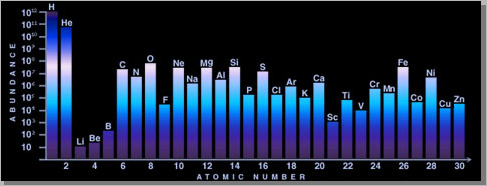
\includegraphics[scale=0.75]{Figures/atomic1.jpg} 
    \caption{Η αφθονία των χημικών στοιχείων στο σύμπαν.}  
    \label{fig:abundace_of_elements}
\end{figure}

Το αποτύπωμα της κοσμικής πυρηνοσύνθεσης βαρέων στοιχείων βρίσκεται και μέσα στην αφθονία των στοιχείων του ηλιακού συστήματος (σχήμα \ref{fig:solar_abundance_of_elements}). Η ηλιακή φωτόσφαιρα και οι μετεωρίτες αντικατοπτρίζουν την χημική υπογραφή του νέφους μέσα από το οποίο γεννήθηκε ο ήλιος. Αυτή η αφθονία όμως, φαίνεται να εκφράζει την γενικότερη συμπεριφορά της δημιουργίας των πυρήνων στο σύμπαν. Αξίζει να παρατηρήσουμε τις κορυφές στα στοιχεία με ατομικούς αριθμούς $A =$ 80, 130 και 195 --οι οποίοι αντιστοιχούν σε μαγικούς αριθμούς-- καθώς η σύνθεση αυτών των στοιχείων προέρχεται αποκλειστικά μέσω των διεργασιών που αναλύουμε στο παράρτημα \ref{apx:nucleosynthesis}.

\begin{figure}
    \centering
    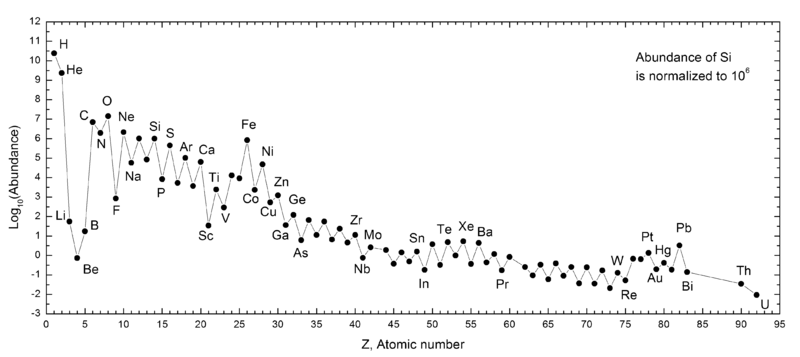
\includegraphics[scale=0.45]{Figures/SolarSystemAbundances.png} 
    \caption{Η αφθονία των χημικών στοιχείων στο ηλιακό μας σύστημα.}
    \label{fig:solar_abundance_of_elements}
\end{figure}

Σχεδόν όλη μάζα των στοιχείων συγκεντρώνεται στα στοιχεία του υδρογόνου και του ηλίου, τα οποία φαίνεται να παρήχθησαν κατά τη γέννηση του σύμπαντος. Η επικράτηση των πυρήνων μικρού ατομικού αριθμού $A$ έναντι των μεγαλυτέρων δεν είναι τυχαία και φαίνεται να οφείλεται σε δυο παράγοντες. Ο ένας παράγοντας είναι ότι σε μεγαλύτερους πυρήνες, η διαδικασία της σύντηξης απαιτεί μεγαλύτερη ενέργεια έτσι ώστε να ξεπεραστεί το απωστικό δυναμικό Coulomb καθώς η πιθανότητα μιας τέτοιας σύντηξης παρουσιάζει εκθετική εξάρτηση του προϊόντος από τα φορτισμένα αντιδρώντα. Για παράδειγμα, η σύντηξη δυο πυρήνων οξυγόνου θα  μας δώσει έναν πυρήνα 64 φορές μεγαλύτερο από εκείνον που θα μας δώσει η σύντηξη δυο πυρήνων υδρογόνου. Ο άλλος παράγοντας φαίνεται να είναι ο αριθμός των νουκλεονίων του πυρήνα. Όπως έχουμε δει και στα παραπάνω διαγράμματα, ο επόμενος εμφανιζόμενος πυρήνας με μονό αριθμό νουκλεονίων μετά το $^{1}$H είναι το $^{25}$Mg που είναι πολύ χαμηλός σε ποσοστά εμφάνισης. Με μια προσεκτικότερη ματιά στις χημικές αναλογίες είναι προφανές ότι υπάρχει μια προτίμηση στη δημιουργία πυρήνων με ζυγό αριθμό νουκλεονίων έναντι σε εκείνους με μονό αριθμό. Επίσης, φαίνεται να υπάρχει σαφής προτίμηση δημιουργίας πυρήνων που έχουν ζυγό-ζυγό αριθμό νουκλεονίων. Για παράδειγμα, στα πρώτα 25 στοιχεία μόνο το $^{14}$N δεν είναι ζυγός-ζυγός πυρήνας, δηλαδή δεν έχει ζυγό αριθμό πρωτονίων και ζυγό αριθμό νετρονίων. Επιπλέον εκτός από τον $^{56}$Fe όλοι οι υπόλοιποι συχνά εμφανιζόμενοι πυρήνες έχουν ζυγούς- ζυγούς πυρήνες αλλά και $Z=N$. Τους πυρήνες με αυτή την ιδιότητα τους ονομάζουμε \textbf{alpha-particle nuclei} εξαιτίας της ομοιότητάς του με τον πρώτο εμφανιζόμενο ζυγό-ζυγό πυρήνα, τον πυρήνα του $^{4}$He. Αυτό εξηγείται μέσω του πυρηνικού μοντέλου φλοιών, δηλαδή στο ότι οι ατομικοί πυρήνες αυξάνουν τις διαστάσεις τους σχηματίζοντας κελύφη γεμάτα με πρωτόνια και νετρόνια. Μόνο συγκεκριμένοι συνδυασμοί αριθμών πρωτονίων και νετρονίων φαίνεται να εμφανίζουν τους ισχυρότερους δεσμούς σύνδεσης και άρα ευσταθή στοιχεία. Τους συνδυασμούς αυτούς τους ονομάζουμε \textbf{μαγικούς αριθμούς}. Πλέον είναι προφανές ότι τα στοιχεία σε μεγαλύτερη αφθονία είναι εκείνα που έχουν διπλά μαγικούς όπως τα: $^{4}$He με $Z = N = 2$, $^{16}$O με $Z = N = 8$, $^{40}$Ca με $Z = N = 20$ και ακόμα και για τον σίδηρο $^{56}$Fe φαίνεται ότι αρχικά δημιουργήθηκε ως τον alpha-particle πυρήνα $^{56}$Ni με $Z = N = 28$. Μετά όμως από τη δημιουργία αυτού του στοιχείου, η διαδιακασία δημιουργίας βαρύτερων στοιχείων φαίνεται να αλλλάζει χαρακτήρα και να προέρχεται από μια διαφορετική διαδιακασία από εκείνη της σύντηξης. Την διαδικασία αυτή θα την αναλύσουμε εκτενώς παρακάτω και δεν είναι άλλη από εκείνη της αρπαγής νετρονίων. Τέλος, στο παρακάτω διάγραμμα Segre (σχήμα \ref{fig:segre_diagram}) φαίνεται μια ολοκληρωμένη εικόνα της τελικής εξέλιξης της πυρηνοσύνθεσης.

\begin{figure}
    \centering
    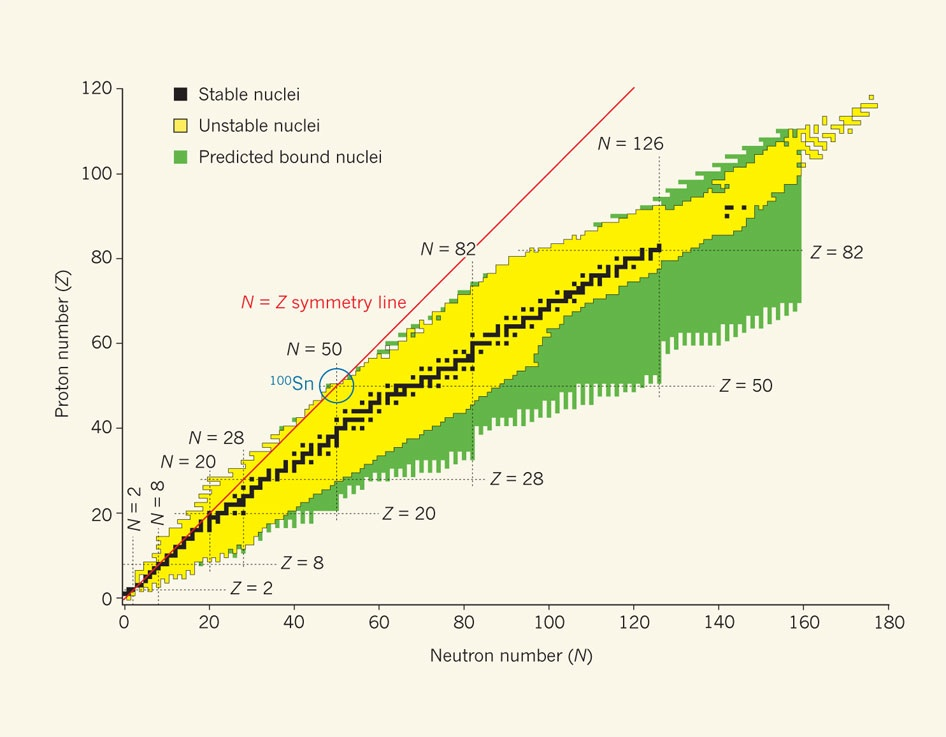
\includegraphics[scale=0.3]{Figures/Nuclei-as-function-of-N-Z.jpg} 
     \caption{Διάγραμμα Segre. Τα στοιχεία που εμφανίζονται με μαύρες κουκκίδες είναι σταθερά ισότοπα και αποτελούν την κοιλάδα σταθερότητας.} 
     \label{fig:segre_diagram}
\end{figure}
%% ---------------------------------------------------------------------------------------------------- %%
%% ---------------------------------------------------------------------------------------------------- %%
%% ---------------------------------------------------------------------------------------------------- %%
\subsection{Δημιουργία πρωτοαστέρων}
Τα άστρα δημιουργούνται κατά κανόνα από τη μεσοαστρική ύλη που υπάρχει στους γαλαξίες και η οποία αποτελείται κυρίως από υδρογόνο, ήλιο, και μοριακή σκόνη. Η ύλη αυτή, όπως και στο αρχέγονο σύμπαν, συχνά σχηματίζει νέφη τεραστίων διαστάσεων και χαμηλής πυκνότητας, τα νεφελώματα. Αυτά τα νέφη εξαιτίας της μεγάλης μάζας τους έχουν και την αντίστοιχη βαρυτική δυναμική ενέργεια, η οποία όμως λόγω της χαμηλής τους πυκνότητας, δεν είναι ικανή να υπερνικήσει τις θερμικές κινήσεις των μορίων και να προκαλέσει τη βαρυτική συστολή και συμπύκνωση.
Ο Jeans έδειξε ότι η δύναμη της πίεσης παύει να αντισταθμίζει τη βαρυτική έλξη, όταν οι διαστάσεις του νέφους είναι μεγαλύτερες, σε τάξη μεγέθους, από το \textbf{μήκος Jeans} που δίνεται απο τη σχέση
\begin{eqnarray}
    \label{eq:jeans_length}
    L_{\text{J}} = \left(\frac{14}{4\pi} \right)^{1/2} \left(\frac{kT}{\mu m_{\text{H}} G \rho} \right)^{1/2}
\end{eqnarray}
Στην περίπτωση αυτή όλη η ύλη, $M_{\text{J}}$, που περιέχεται σε μία σφαίρα με ακτίνα $L_{\text{J}}$, η οποία ισούται με
\begin{equation}
    \label{eq:jeans_mass}
    M_{\text{J}} = \frac{4}{3} \pi \rho L_{\text{J}} = \left(\frac{3}{4\pi \rho} \right)^{1/2} \left( \frac{5kT}{\mu m_{\text{H}} G} \right)^{3/2}
\end{equation}
συμπυκνώνεται και δημιουργεί ένα αστρικό αντικείμενο. Συμπερασματικά, η συμπύκνωση ευνοείται όταν η θερμοκρασία είναι μικρή, και η πυκνότητα μεγάλη. Ανάλογα με το μέγεθος της μάζας (το οποίο εξαρτάται από τη θερμοκρασία, την πυκνότητα και το μέσο μοριακό βάρος του αερίου), το αντικείμενο αυτό μπορεί να είναι ένας αστέρας, ένα σμήνος αστέρων ή και ένας γαλαξίας.

Για να εγκαταλείψει το νεφος την ισορροπία και να αρχίσει η συστολή απαιτείται μια αρχική διαταραχή, μήκους κύματος μεγαλύτερου ή ίσου με το χαρακτηριστικό μήκος Jeans γι' αυτό το νέφος. Διάφοροι παράγοντες μπορεί να επιφέρουν την βαρυτική κατάρρευση, μερικοί από τους οποίους είναι
  
  \begin{itemize}
  \item \textbf{Σύγκρουση Νεφών}\\
  Κατά τη σύγκρουση δυο ή περισσοτέρων νεφών η πυκνότητά τους αυξάνεται τοπικά δημιουργώντας έτσι περιοχές αστρογέννησης.
  
  \item \textbf{Έκρηξη Υπερκαινοφανούς Αστέρα (supernova)}\\
Όπως θα αναφέρουμε και παρακάτω, το τέλος ενός αστέρα μεγάλης μάζας συνοδεύται από την έκρηξή του. Σε μία τέτοια έκρηξη, το μεγαλύτερο μέρος ενός αστεριού (ή και ολόκληρο το αστέρι) διαλύεται και η ύλη του εκσφενδονίζεται βίαια στο διάστημα. Το ωστικό κύμα αυτής της έκρηξης συμπιέζει τα γειτονικά νέφη και δίνει το έναυσμα για τη βαρυτική συστολή.

  \item \textbf{Ύπαρξη νεαρών αστέρων μεγάλης μάζας}\\
 Όταν στην περιοχή των νεφών έχουν ήδη σχηματισθεί νέα μεγάλα αστέρια, αυτά εκπέμπουν τεράστια ποσά ακτινοβολίας η πίεση της οποίας επιδρά πάνω στην ύλη των γειτονικών νεφών και κάτω από τις κατάλληλες συνθήκες μπορεί να επιφέρει βαρυτική κατάρρευση.
 
 \item \textbf{Σπειροειδή Κύματα Πυκνότητας}\\
Σύμφωνα με τη θεωρία κυμάτων πυκνότητας (Lin και Shu, 1963), σπειροειδή κύματα πυκνότητας ξεκινούν από τον πυρήνα του γαλαξία και ξετυλίγονται προς τα έξω στον γαλαξιακό δίσκο. Τα κύματα αυτά συμπιέζουν το αέριο του δίσκου στα σημεία διεύλευσής τους προκαλώντας τη βαρυτική συστολή των μεσοαστρικών νεφών και τη δημιουργία νέων άστρων. Σε κάθε περίπτωση η παρουσία της πίεσης είναι απαραίτητη για να υπερνικηθούν οι τυχαίες θερμικές κινήσεις των μορίων.
\end{itemize}

Αυτή η βαρυτική κατάρρευση έχει ως επακόλουθο την εξώθερμη σύντηξη του υδρογόνου. Από τη στιγμή που σε ένα αστέρι ξεκινήσουν οι  θερμοπυρηνικές αντιδράσεις στον πυρήνα του, αρχίζει να ακτινοβολεί έντονα και ξεκινάει τη "ζωή" του. Αστέρια με μεγάλη μάζα έχουν μεγάλη βαρύτητα, συνεπώς μεγάλη πίεση και θερμοκρασία στον πυρήνα τους. Έτσι, οι συγκρούσεις μεταξύ των πυρήνων υδρογόνου είναι συχνότερες με αποτέλεσμα ο ρυθμός μεταστοιχείωσης του υδρογόνου να είναι μεγάλος. Επομένως, η παραγωγή και η ακτινοβολία ενέργειας είναι επίσης μεγάλες, έτσι ώστε τα αστέρια με μεγάλη μάζα να έχουν μεγάλη επιφανειακή θερμοκρασία και λαμπρότητα. Αντιθέτως, αστέρια με μικρή μάζα ακτινοβολούν λιγότερο. Οι μάζες των αστεριών ποικίλουν αλλά εντός συγκεκριμένων ορίων ($0.08 M_{\odot}<M<150 M_{\odot}$).
%% ---------------------------------------------------------------------------------------------------- %%
%% ---------------------------------------------------------------------------------------------------- %%
%% ---------------------------------------------------------------------------------------------------- %%
\subsubsection{Γραμμή Hayashi}
Η γενικά παραδεκτή σήμερα θεωρία εξέλιξης των πρωτοαστέρων είναι αυτή που πρότεινε ο Ιάπωνας αστρονόμος Hayashi. Στην αρχή το μεσοαστρικό νέφος που συστέλελται είναι οπτικά διαφανές (οπτικό βάθος $\tau \ll 1$) επειδή η πυκνότητά του είναι μικρή. Έτσι η ενέργεια που παράγεται στο εσωτερικό του, λόγω της βαρυτικής συστολής, ακτινοβολείται ελεύθερα στο μεσοαστρικό χώρο. Κατά τη διάρκεια αυτής της φάσης η θερμοκρασία στο εσωτερικό του νέφους παραμένει σταθερή και ίση με την αρχική, δηλαδή της τάκης των $10 \,\text{K}$. Γρήγορα, όμως, η πυκνότητα αυξάνει σημαντικά (καταρχήν στο κέντρο και αργότερα στις υπόλοιπες περιοχές), οπότε η ύλη παύει να είναι πια διαφανής. Στις περιοχές που η πυκνότητα ξεπερνά κάποια οριακή τιμή, η ύλη γίνεται αδιαφανής ($\tau \approx 1$) και η θερμοκρασία αυτών των περιοχών αρχίζει να αυξάνει, επειδή η παραγόμενη, λόγω συστολής, ενέργεια δεν μπορεί να ακτινοβοληθεί ελεύθερα στο μεσοαστρικό χώρο. Έτσι αυξάνει, καταρχήν, η θερμοκρασία της επιφάνειας του "πυρήνα" του νέφους, από όπου προέρχεται και η ακτινοβολία που εκπέμπει ο πρωτοαστέρας.

Σύμφωνα λοιπόν με τα παραπάνω, το αρχικό νέφος αρχίζει να εκπέμπει φως, ενώ έχει ακόμη μεγάλες διαστάσεις και είναι ακόμη ψυχρό. Επομένως βρίσκεται στην επάνω δεξιά γωνία του διαγράμματος H-R. Καθώς το νέφος συστέλλεται, η λαμπρότητά του ελλατώνεται (επειδή ελλατώνεται η ακτίνα του) η δε θερμοκρασία της ακτινοβολούσας επιφάνειας παραμένει περίπου σταθερή (αρχική καθοδική πορεία στο σχήμα \ref{fig:hayashi_tracks}). Καθώς όμως η βαρυτική κατάρρευση συνεχίζεται, κάποτε η θερμοκρασία της ακτινοβολούσας επιφάνειας αρχίζει να αυξάνει σημαντικά, οπότε μεγαλώνει και η φωτεινότητα του πρωτοαστέρα. Στο διάγραμμα H-R ο αστέρας ακολουθεί την ανοδική πορεία της καμπύλης στο σχήμα \ref{fig:hayashi_tracks}.
\begin{figure}[h!]
    \centering
    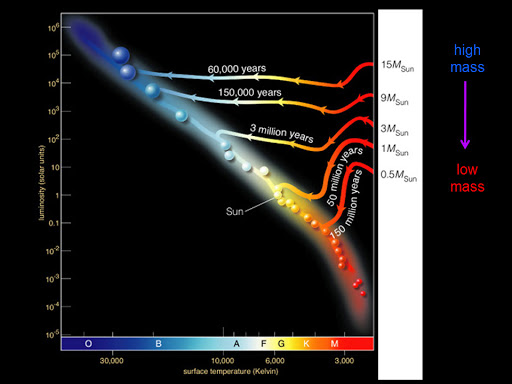
\includegraphics[scale=0.5]{Figures/hayashi_tracks.jpg}
    \caption{Πορείες Hayashi για πρωτοαστέρες διαφόρων μαζών και εγκατάστασή τους στην κύρια ακολουθία.}
    \label{fig:hayashi_tracks}
\end{figure}

Με την πάροδο του χρόνου αυξάνει και η πυκνότητα των εξωτερικών στρωμάτων, με αποτέλεσμα να γίνουν αδιαφανή σε οπτικά μήκη κύματος, ώστε η ακτινοβολία του πυρήνα να μην μπορεί να τα διαπεράσει πλέον. Επομένως, η ακτινοβολούσα επιφάνεια τείνει να συμπέσει με την τελική επιφάνεια του αστέρα. Από τη στιγμή αυτή και μετά, συμβαίνουν δύο βασικά γεγονότα:
\begin{enumerate}
    \item Η συστολή του πρωτοαστέρα συνεχίζεται, αν και με βραδύτερο ρυθμό, και επομένως η επιφάνειά του και η φωτεινότητά του ελλατώνονται (καθοδικό τμήμα της καμπύλης για πρωτοαστέρες με μικρή μάζα στο σχήμα \ref{fig:hayashi_tracks}.
    \item Η θερμοκρασία του πυρήνα αυξάνει σημαντικά, με αποτέλεσμα να αρχίσουν οι πρώτες θερμοπυρηνικές αντιδράσεις.
\end{enumerate}

Κατά τη διάρκεια της καύσης των διάφορων στοιχείων έχουμε ανάσχεση της βαρυτικής συστολής, επειδή η θερμική πίεση του αερίου αντισταθμίζει τη βαρυτική πίεση. Τα ελαφρά στοιχεία D, Li, Be, και B, τα οποία μεταστοιχειώνονται σε χαμηλές θερμοκρασίες, εξαντλούνται γρήγορα επειδή, όπως γνωρίζουμε από μετρήσεις της σχετικής αφθονίας των διάφορων στοιχείων στη φύση, είναι πολύ σπάνια. Όταν η θερμοκρασία φτάσει τους $\sim 10^7 \,\text{K}$, αρχίζει η καύση του άφθονου υδρογόνου σύμφωνα με τη σχέση \eqref{eq:4p_he4} και επιτυγχάνεται θερμική και υδροστατική ισορροπία. Ο αστέρας αρχίζει τη σταδιοδρομία του στην κύρια ακολουθία. Όσο πιο μεγάλη μάζα έχει ένας αστέρας όταν φτάσει στην κύρια ακολουθία, τόσο πιο θερμός και πιο φωτεινός είναι. Επομένως οι αστέρες μεγάλης μάζας εγκαθίστανται στο πάνω αριστερό τμήμα της κύριας ακολουθία, ενώ οι αστέρες μικρής μάζας στο κάτω δεξιό.

Η στιγμή της έναρξης της μεταστοιχείωσης του υδρογόνου στον πυρήνα ενός αστέρα, που συμπίπτει με την εγκατάστασή του στην κύρια ακολουθία, θεωρείται ως η αρχή της ζωής του, αντιστοιχεί δηλαδή σε μηδενική ηλικία. Η πορεία, στο διάγραμμα H-R, που ακολούθησε ο πρωτοαστέρας από τη στιγμή της δημιουργίας του μέχρι να φθάσει στη φάση ενός αστέρα μηδενικής ηλικίας ονομάζεται \textbf{πορεία Hayashi} (Hayashi track). Ο γεωμετρικός τόπος των θέσεων όλων των αστέρων μηδενικής ηλικίας στο διάγραμμα H-R ονομάζεται \textbf{κύρια ακολουθία μηδενικής ηλικίας} (zero age main sequence -- ZAMS). Το χρονικό διάστημα που μεσολαβεί από τη στιγμή της δημιουργίας του πρωτοαστέρα μέχρι τη στιγμή της εγκατάστασής του στην κύρια ακολουθία εξαρτάται από τη μάζα του: είναι μεγάλο για πρωτοαστέρες μικρής μάζας και μικρό για πρωτοαστέρες μεγάλης μάζας. Για τον Ήλιο αυτό το διάστημα υπολογίζεται ότι ήταν $\sim 2 \times 10^7 \,\text{yr}$. Από τα παραπάνω γίνεται σαφής και η διαφορά της ZAMS από την κύρια ακολουθία ενός σμήνους αστέρων: η ZAMS αποτελείται από τις θέσεις των αστέρων \textit{τη στιγμή της δημιουργίας τους}, ενώ η κύρια ακολουθία ενός συνόλου αστέρων (π.χ. ενός σμήνους) αποτελείται από θέσεις αστέρων \textit{διάφορων ηλικιών}, έστω και αν οι αστέρες αυτοί προέρχονται από πρωτοαστέρες που δημιουργήθηκαν ταυτόχρονα, αφού αστέρες διαφόρων μαζών χρειάζονται διαφορετικά χρονικά διαστήματα για να εγκατασταθούν στην κύρια ακολουθία. Επομένως, η ZAMS είναι ένα από πρότυπο χρήσιμο κυρίως για θεωρητικούς υπολογισμούς.
%% ---------------------------------------------------------------------------------------------------- %%
%% ---------------------------------------------------------------------------------------------------- %%
%% ---------------------------------------------------------------------------------------------------- %%
\subsection{Εξέλιξη μετά την κύρια ακολουθία}
Στο μεγαλύτερο μέρος της ζωής τους, οι αστέρες "καίνε" το υδρογόνο τους μετατρέποντάς το σε ήλιο σύμφωνα με τον κύκλο "πρωτονίου-πρωτονίου" (proton-proton chain) ή με τον κύκλο άνθρακα (κύκλος CNO). Όταν ένα σημαντικό ποσοστό του $^1$H μεταστοιχειωθεί σε $^4$He, ο ρυθμός των θερμοπυρηνικών αντιδράσεων ελαττώνεται και γίνεται μικρότερος από το ρυθμό ακτινοβολίας της επιφάνειας του άστρου. Έτσι, υπό την επίδραση της βαρύτητας και μέσω του μηχανισμού Kelvin-Helmholtz, η θερμοκρασία αυξάνεται και ξεκινά  η καύση του $^4$He προς $^{12}$C, με την προϋπόθεση η μάζα του αστέρα να είναι μεγαλύτερη των 0.4 ηλιακών μαζών.

 Η ενέργεια που παράγεται στον πυρήνα εξωθεί τα υπερκείμενα στρώματα με αποτέλεσμα την τεράστια διόγκωση του αστέρα και τη μετατροπή του σε ερυθρό γίγαντα. Αστέρες με μάζα ίση περίπου με την ηλιακή, κατά τη φάση του ερυθρού γίγαντα, χάνουν σε διάστημα 1000 ετών το 20\% με 30\% της μάζας τους σχηματίζοντας τελικά ένα \textit{πλανητικό νεφέλωμα}. Από την φάση του ερυθρού γίγαντα και μετά, ανάλογα με την μάζα ενός αστέρα διαφοροποιείται και η εξέλιξή του. 
%% ---------------------------------------------------------------------------------------------------- %%
%% ---------------------------------------------------------------------------------------------------- %%
%% ---------------------------------------------------------------------------------------------------- %%
\subsubsection{Αστέρες μικρής μάζας}
H συρρίκνωση του αδρανή (αστρικού) πυρήνα $^4$He συνεχίζεται με ταυτόχρονη παραγωγή ενέργειας, μέσω του μηχανισμού Kelvin-Helmholtz, μέχρι τη στιγμή που η αριθμητική πυκνότητα των ηλεκτρονίων σε αυτόν γίνει τόση ώστε αυτά να βρίσκονται σε κατάσταση εκφυλισμού. Για αστέρες με μάζα μικρότερη των $0.8 M_{\odot}$ αυτό συμβαίνει όσο η θερμοκρασία του πυρήνα είναι μικρότερη από τη θερμοκρασία "ανάφλεξης" του $^4$He. Ο αστρικός πυρήνας σταθεροποιείται σε αυτή την κατάσταση και μετατρέπεται σε έναν λευκό νάνο ηλίου. Τα υπόλοιπα στρώματα του αστέρα συνεχίζουν τη διαστολή τους με επιταχυνόμενο ρυθμό,  αντλώντας ενέργεια από την καύση του $^1$H στον φλοιό του αστέρα. Ταυτόχρονα όμως, η βαρυτική έλξη του πυρήνα γίνεται ασθενέστερη καθώς αυτά απομακρύνονται. Σε αυτό το σημείο, ο αστέρας περνά στην φάση του ερυθρού υπεργίγαντα. Κατά τη διάρκεια αυτού του σταδίου, ο αστέρας "σκορπίζεται" στην ευρύτερη περιοχή μέσω του έντονου αστρικού ανέμου που εμφανίζει, δημιουργώντας γύρω του ένα πλανητικό νεφέλωμα. To τελικό αποτέλεσμα είναι ένας λευκός νάνος θερμοκρασίας της τάξης των $30000 \,\text{K}$ που αποτελείται κυρίως από $^4$He και λίγο $^1$H.

%% ---------------------------------------------------------------------------------------------------- %%
%% ---------------------------------------------------------------------------------------------------- %%
%% ---------------------------------------------------------------------------------------------------- %%
\subsubsection{Αστέρες ενδιάμεσης μάζας}
Σε αυτή την κατηγορία έχουμε αστέρες με μάζα που βρίσκεται στο εύρος $0.8 \,M_{\odot} < M < 3 \,M_{\odot}$.
H εξέλιξη αυτών των αστέρων ακολουθεί την πορεία αυτών των μικρότερης μάζας εώς το στάδιο του ερυθρού γίγαντα. Σε αυτή την περίπτωση όμως, η δύναμη της βαρύτητας είναι σημαντικά ισχυρότερη με αποτέλεσμα τα ηλεκτρόνια του αδρανούς πυρήνα $^4$He να εκφυλίζονται και η θερμοκρασία του πυρήνα να ξεπερνά τη θερμοκρασία ανάφλεξης του $^4$He ($2\times 10^{8}K$). Τότε αρχίζει η καυση του $^4$He μέσω της διαδικασίας τριων-α που συζητήσαμε παραπάνω. Όταν όλο το $^4$He που βρίσκεται στον πυρήνα εξαντληθεί έχοντας μετατραπεί σε $^{12}$C και $^{16}$O, ξεκινά η καύση του $^4$He που εντοπίζεται στον εξωτερικό φλοιό του αστρικού πυρήνα, ενώ αυτός περιβάλλεται από έναν φλεγόμενο φλοιό $^1$H ακολουθώντας στο διάγραμμα H-R τον ασυμπτωτικό κλάδο των ερυθρών γιγάντων. Η τελική κατάσταση ενός τέτοιου αστέρα είναι η δημιουργία ενός λευκού νάνου άνθρακα-οξυγόνου.
%% ---------------------------------------------------------------------------------------------------- %%
%% ---------------------------------------------------------------------------------------------------- %%
%% ---------------------------------------------------------------------------------------------------- %%
\subsubsection{Αστέρες μεγάλης μάζας}
Η εξέλιξη αστέρων με μάζα μεγαλύτερη των $3M_{\odot}$ διαφέρει πλέον σημαντικά. Η χαρακτηριστικότερη διαφορά είναι ότι, μετά την εξάντληση των αποθεμάτων άνθρακα και οξυγόνου η θερμοκρασία του πυρήνα είναι πολύ υψηλή και ξεκινάει η μεταστοιχείωσή τους στο επόμενο βαρύτερο στοιχείο, το πυρίτιο (Si). Όσο μεγαλύτερη είναι η μάζα του πυρήνα, οι διαδοχικές μεταστοιχειώσεις προχωρούν μέχρι τη δημιουργία του σιδήρου (Fe). Σε αυτό το σημείο, η διαδικασία διακόπτεται καθώς η περαιτέρω μεταστοιχείωση του σιδήρου είναι μια ενδόθερμη αντίδραση και έτσι η αλυσίδα των συντήξεων σταματά. Σε αυτό το στάδιο, η δομή ενός αστέρα θυμίζει αυτή ενός κρεμμυδιού (onion-like structure) καθώς αποτελείται από πολλά διαφορετικά στρώματα-φλοιούς.
\begin{figure}[h!]
    \centering
    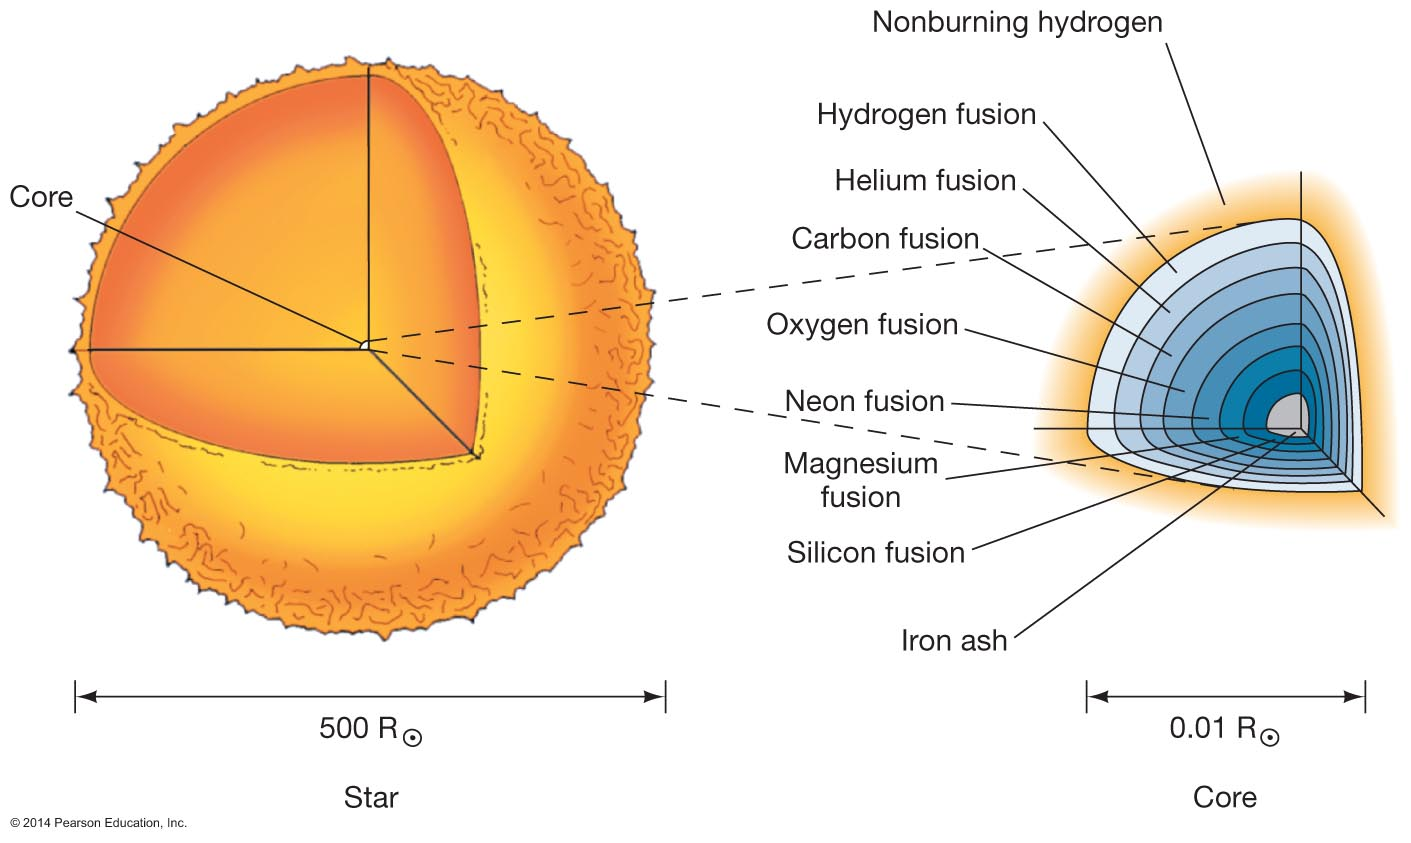
\includegraphics[scale=0.4]{Figures/onion_stellar_structure.jpg}
    \caption{Η δομή "κρεμμυδιού" και η καύση στοιχείων ανά φλοιό κατά τα τελευταία στάδια ζωής ενος αστέρα.}
    \label{fig:onion_stellar_structure}
\end{figure}

Η συνέχεια είναι σε κάθε περίπτωση --κυριολεκτικά-- καταστροφική για τον αστέρα. Με τις σημερινές γνώσεις που έχουμε στην αστροφυσική πιστεύουμε ότι μπορούν να υπάρξουν τέσσερις μόνο τελικές καταστάσεις στις οποίες είναι δυνατόν να καταλήξει ένας αστέρας όταν σταματήσει οριστικά η παραγωγή ενέργειας στον πυρήνα του: 

\begin{itemize}
\item Πλήρης διάλυση του αστέρα
\item Δημιουργία λευκού νάνου
\item Δημιουργία αστέρα νετρονίων
\item Δημιουργία μελανής οπής
\end{itemize}

 Η παραγωγή βαρύτερων στοιχείων του σιδήρου ξεκινά σε κάποιο από τα παραπάνω τελικά στάδια του αστέρα, με διάφορες διεργασίες που μπορούν να λάβουν χώρα και στις οποίες αναφερόμαστε εκτενώς στο παράρτημα \ref{apx:nucleosynthesis}.
%% ---------------------------------------------------------------------------------------------------- %%
%% ---------------------------------------------------------------------------------------------------- %%
%% ---------------------------------------------------------------------------------------------------- %%
\subsubsection{Εξέλιξη στο διάγραμμα H-R}
Η εξέλιξη αστέρων χαμηλής μάζας μπορεί να περιγραφεί ποιοτικά με τη βοήθεια του διαγράμματος H-R ενός σφαιρωτού σμήνους (σχήμα \ref{fig:hrd_evolution}. Παρόλο που το διάγραμμα H-R ενός σμήνους αποτελεί ένα στιγμιότυπο σε μία συγκεκριμένη χρονική στιγμή, παρουσιάζει όλα τα εξελικτικά στάδια στη ζωή ενός αστέρα καθώς η διάρκεια παραμονής ενός αστέρα σε κάθε εξελικτική φάση εξαρτάται από τη μάζα του.

\begin{figure}
    \centering
    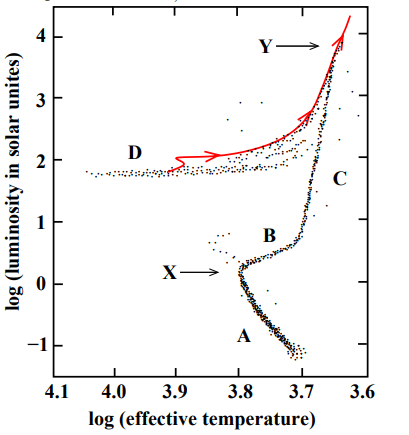
\includegraphics[scale=0.6]{Figures/hrd_evolution.png}
    \caption{Εξέλιξη αστέρων χαμηλής μάζας σε ένα σφαιρωτό σμήνος.}
    \label{fig:hrd_evolution}
\end{figure}

\begin{itemize}
    \item \textbf{Περιοχή A}: Παριστάνει την κύρια ακολουθία. Όλα τα αστέρια σε αυτή την περιοχή είναι στη φάση της κεντρικής καύσης του υδρογόνου, η οποία είναι και η μεγαλύτερη σε χρονική διάρκεια φάση στην ζωή του αστέρα. Αστέρες με χαμηλότερη λαμπρότητα κατά μήκος της κύριας ακολουθίας έχουν χαμηλότερη μάζα καθώς εγκαταστάθηκαν εκεί από διαφορετική πορεία Hayashi.
    \item \textbf{Σημείο στροφής X}: Αστέρες κοντά σε αυτό το σημείο έχουν (σχεδόν) εξαντλήσει το απόθεμα του υδρογόνου στον πυρήνα τους και είναι έτοιμα να αναπτύξουν, πρώτα έναν ισοθερμικό, και έπειτα έναν ηλεκτρονιακά εκφυλισμένο πυρήνα, αφήνωντας πίσω τους την κύρια ακολουθία με το να μετακινηθούν προς χαμηλότερες θερμοκρασίες (δηλαδή την περιοχή B). Παρατηρήστε ότι υπάρχουν μερικά άστρα στην προέκταση της κύριας ακολουθίας, μετά το σημείο στροφής X. Αυτοί οι αστέρες ονομάζονται "κυανοί περιπατητές" (blue stragglers) και είναι ελαφρώς πιο μεγάλοι (σε μάζα) αστέρες που δεν έχουν εξελιχθεί ακόμα πέρα από την κύρια ακολουθία. Αυτά τα αστέρια είναι πιθανόν το αποτέλεσμα των αλληλεπιδράσεων με κάποιο συνοδό αστέρα, ή δημιουργήθηκαν με τη σύγκρουση και συγχώνευση με κάποιο άλλο άστρο στο σφαιρωτό σμήνος (κάτι που συμβαίνει αρκετά συχνά στα πυκνά σφαιρωτά σμήνη).
    \item \textbf{Περιοχές B και C}: Με την έξοδό τους από την κύρια ακολουθία, οι αστέρες γίνονται μεγαλύτεροι (σε διαστάσεις) και πιο λαμπροί και μεταμορφώνονται σε υπογίγαντες (περιοχή B) και τελικά σε γίγαντες (περιοχή C). Στη φάση των γιγάντων, εξελίσσονται με σχεδόν σταθερή ενεργό θερμοκρασία $T_{\text{eff}}$. Σε αυτή τη φάση, οι αστέρες έχουν έναν εκφυλισμένο συμπαγή πυρήνα ο οποίος περιτριγυρίζεται από μία ατμόσφαιρα (convective envelope) που καταλαμβάνει τον μεγαλύτερο όγκο του αστέρα. Η καύση του υδρογόνου συνεχίζεται σε έναν φλοιό που περιβάλλει τον πυρήνα.  
    \item \textbf{Σημείο στροφής Y}: Σε αυτό το σημείο ξεκινάει η καύση του ηλίου στον πυρήνα του αστέρα. Επειδή ο πυρήνας αποτελείται από εκφυλισμένο αέριο ηλεκτρονίων, η ανάφλεξη του ηλίου είναι βίαιη και οδηγεί σε αναπροσαρμογή της δομής του αστέρα (έκλαμψη ηλίου -- helium flash). Παρόλα αυτά, η εκλαμψη δεν είναι αρκετά εκρηκτική για να διαλύσει τον αστέρα. Αντ' αυτού, ο αστέρας επαναπροσαρμόζει τη δομή του και καταλήγει στον οριζόντιο κλάδο του διαγράμματος (περιοχή D). Γι' αυτό, η έκλαμψη ηλίου σηματοδοτεί μία προσωρινή αύξηση στην λαμπρότητα του αστέρα, ορίζοντας την κορυφή του κλάδου των γιγάντων.
    \item \textbf{Περιοχή D}: Αφού επανέλθει σε κατάσταση υδροστατικής και θερμικής ισορροπίας, ο αστέρας περνάει σημαντικό μέρος της ζωής του στον οριζόντιο κλάδο, όπου καίει τα αποθέματα ηλίου στον πυρήνα του, ο οποίος είναι περιτριγυρισμένος από έναν φλοιό στον όποιο πραγματοποιείται καύση υδρογόνου (αυτή είναι συνήθως και η κύρια πηγή ενέργειας). Όταν εξαντληθούν τα αποθέματα του ηλίου στο κέντρο του αστέρα, επιστρέφει στη φάση του ερυθρού γίγαντα με την πορεία που ακολουθεί να προσεγγίζει ασυμπτωτικά τον αρχικό κλάδο των γιγάντων. Σε αυτή την ασυμπτωτική φάση (AGB phase), ο αστέρας έχει έναν εκφυλισμένο πυρήνα που αποτελείται από άνθρακα και οξυγόνο, και περιτριγυρίζεται από έναν φλοιό πλούσιο σε ήλιο και μία πλούσια σε υδρογόνο ατμόσφαιρα. Η πηγή ενέργειας είναι η θερμοπυρηνική σύντηξη του υδρογόνου και του ηλίου που συμβαίνουν σε λεπτούς σφαιρικούς φλοιούς γύρω από τον αδρανή εκφυλισμένο πυρήνα. 
    Επειδή σε αυτό το στάδιο, η ένταση του αστρικού ανέμου είναι πολύ μεγάλη, ο αστέρας χάνει τα εξωτερικά του στρώματα εκθέτοντας τους φλοιούς στους οποίους έχουμε ακόμα καύση. Ο αστέρας έχει πλέον περάσει στη φάση του πλανητικού νεφελώματος στο διάγραμμα H-R και αρζίσει να κινείται προς υψηλότερες θερμοκρασίες με περίπου σταθερή λαμπρότητα. Αυτό συμβαίνει επειδή αρχίζουμε και βλέπουμε πλέον τον πυρήνα του αστέρα που είναι θερμός ενώ η παραγωγή ενέργειας στους φλοιούς παραμένει η ίδια.
    Σε κάποια φάση, η πυρηνική καύση στους φλοιούς θα σταματήσει και ο αστέρας θα αποτινάξει τελείως την ατμόσφαιρά του εκθέτοντας τον πυρήνα του (λευκός νάνος), ο οποίος θα συνεχίσει να ψύχεται εως ότου φτάσει σε θερμική ισορροπία με το υπόλοιπο Σύμπαν.
\end{itemize}
%% ---------------------------------------------------------------------------------------------------- %%
%% ---------------------------------------------------------------------------------------------------- %%
%% ---------------------------------------------------------------------------------------------------- %%
%     \chapter{Αστρικά κατάλοιπα}
\label{ch:Chapter6}

Όταν σταματήσουν οι θερμοπυρηνικές αντιδράσεις στο εσωτερικό των άστρων, τότε ο πυρήνας αρχίζει να ψύχεται, επειδή δεν αναπληρώνονται τα ποσά της ενέργειας που ρέουν προς τα εξωτερικά στρώματα του αστέρα. Η ψύξη του πυρήνα, όμως, συνεπάγεται πτώση της θερμικής πίεσης στο εσωτερικό του, οπότε η πίεση των υπερκείμενων στρωμάτων αρχίζει να υπερισχύει της θερμικής πίεσης του αερίου, με αποτέλεσμα ο πυρήνας να αρχίσει να συστέλλεται. Αν η μάζα του είναι μικρή ($M < 1\,M_\odot$), η συστολή του δεν συνοδεύεται, συνήθως, από καταστροφικά φαινόμενα. Αντίθετα, η ύλη αστέρων μεγάλης μάζας υφίσταται καταστροφική "κατάρρευση", η οποία συνήθως ακολουθείται από έκρηξη, και η ισορροπία των δυνάμεων που διέπουν την ύπαρξη της τελικής κατάστασης, στην οποία θα περιπέσουν αυτοί οι αστέρες, είναι πολύ λεπτή.

Με τις σημερινές γνώσεις της Φυσικής πιστεύουμε ότι είναι δυνατόν να υπάρξουν τριών ειδών τελικές καταστάσεις, όταν σταματήσει οριστικά η παραγωγή ενέργειας από θερμοπυρηνικές αντιδράσεις, στις οποίες γενικά αναφερόμαστε ως \textbf{συμπαγείς αστέρας} (compact stars) επειδή έχουν μικρές τυπικές διαστάσεις και μεγάλες πυκνότητες. Μία τέταρτη περίπτωση κατά την οποία ο αστέρας διαλύεται, με την ύλη να διασκορπίζεται στο μεσοαστρικώ χώρο χωρίς να αφήνει πίσω κάποιο κατάλοιπο, θα ζηζητηθεί στο Κεφάλαιο \ref{ch:Chapter7}.


\section{Λευκοί νάνοι}
{\color{red} \hrule}
Λευκός νάνος είναι ο εκφυλισμένος, γυμνός πυρήνας ενός αστέρα με σχετικά μικρή αρχική μάζα ($M \leq 5\,M_\odot$). Αρχικά, ο λευκός νάνος έχει πολύ υψηλή θερμοκρασία. Με την πάροδο του χρόνου, όμως, η θερμοκρασία του συνεχώς μειώνεται, μέχρις ότου πάψει να ακτινοβολεί θερμικά. Στην περίπτωση αυτή η υδροστατική ισορροπία του αστέρα εξασφαλίζεται από την (κβαντομηχανικής και όχι θερμικής προέλευσης) πίεση των ηλεκτρονίων. \\
{\color{red} \hrule}




\section{Αστέρες νετρονίων}
{\color{red} \hrule}
Αστέρας νετρονίων είναι ο εκφυλισμένος, γυμνός πυρήνας ενός αστέρα με σχετικά μεγάλη αρχική μάζα. Η εξέλιξη της θερμοκρασίας του ακολουθεί, όπως πιστεύουμε σήμερα, την πορεία της θερμοκρασίας των λευκών νάνων. Σ' αυτήν την περίπτωση η υδροστατική ισορροπία εξασφαλίζεται από την κβαντομηχανικής φύσεως πίεσης των νετρονίων. Δεν αποκλείεται ενάς τέτοιος αστέρας να παρουσιαστεί ενεργά στον ουρανό υπό την μορφή ενός pulsar, που γίνεται ορατός με παρατηρήσεις σε ραδιαφωνικά, κυρίως, μήκη κύματος.\\
{\color{red} \hrule}





\section{Μαύρες τρύπες}




{\color{red} \hrule}
Στην περίπτωση των μελανών οπών, η υδροστατική ισορροπία του αστέρα έχει καταστραφεί, επειδή η διαθέσιμη πίεση (θερμικής ή κβαντομηχανικής προέλευσης) δεν είναι ικανή να αντισταθμίσει την βαρυτική. Η μάζα του αστέρα έχει καταρρεύσει, δημιουργώντας ένα αντικείμενο εξαιρετικά μεγάλης πυκνότητας. Σε κάθε μελανή οπή μπορούμε να αντιστοιχήσουμε ένα χαρακτηριστικό μήκος, $R_S$, που ονομάζεται ακτίνα Schwarzschild, με τη σχέση $R_S = 2GM/c^2$. Το βαρυτικό πεδίο μιας μελανής οπής είναι τόσο ισχυρό, ώστε σε απόσταση μικρότερη από την ακτίνα Schwarzschild ακόμα και το φως δεν μπορεί να διαφύγει από την βαρυτική έλξη.\\
{\color{red} \hrule}


%     \chapter{Διπλά συστήματα \& Μεταβλητοί αστέρες}
\label{ch:Chapter7}
{\hypersetup{linkcolor=black, pdfborder=0 0 1}
	\minitoc
	%\newpage
}

\section{Διπλά συστήματα αστέρων}


\underline{Διπλό σύστημα αστέρων}: {\color{blue}δύο αστέρες που αλληλεπιδρούν βαρυτικά και το σύστημα είναι δέσμιο.} Αν ένας αστέρας έχει μεγάλη ταχύτητα και περάσει από την γειτονιά ενός άλλου αστέρα, τότε τα 2 αστέρια θα αλληλεπιδράσουν βαρυτικά μεν, αλλά το σύστημα δεν θα είναι δέσμιο.

Το ότι το σύστημα είναι δέσμιο σημαίνει ότι η ενέργεια του συστήματος είναι αρνητική (θετική κινητική ενέργεια προφανώς, αλλά αρνητική δυναμική). Επίσης ισχύουν τα εξής:

\begin{itemize}
    \item Οι αστέρες εκτελούν ελλειπτικές τροχιές γύρων από το κέντρο μάζας (ΚΜ) του συστήματος.
    \item Το επίπεδο και η περίοδος της τροχιάς είναι κοινά και για τα δύο αστέρια.
    \item το ΚΜ βρίσκεται στην ευθεία που ενώνει τα δύο αστέρια, και η θέση του σ' αυτή καθορίζεται από την σχέση:
        \begin{equation}
            \label{eq:center_mass}
            \frac{a_B}{a_A} = \frac{M_A}{M_B}
        \end{equation}
        όπου $a_A, a_B$ είναι οι αποστάσεις των αστέρων από το ΚΜ.
    \item Για την περίοδο των τροχιών των αστέρων, P, ισχύει ο 3ος νόμος του Kepler
        \begin{equation}
            \label{eq:Kepler_third_law}
            P^2 = \frac{4\pi^2}{G}a^3 \frac{1}{(M_A + M_B)}
        \end{equation}
        όπου $a$ είναι ο μεγάλος ημιάξονας της τροχιάς της \textit{σχετικής} θέσης των δύο αστέρων.
\end{itemize}

Αν γνωρίζουμε λοιπόν τα χαρακτηριστικά του συστήματος (γωνία κλίσης επιπέδου τροχιάς, $P, a_B, a_A, a$) τότε έχουμε ένα σύστημα 2 εξισώσεων (τις σχέσεις \eqref{eq:center_mass} και \eqref{eq:Kepler_third_law}) για 2 αγνώστους ($M_A$, $M_B$).  Έτσι, μπορούμε να υπολογίσουμε τις μάζες των δύο αστέρων.






\subsection{Κατηγορίες διπλών συστημάτων}
Τα διπλά συστήματα αστέρων κατηγοριοποιούνται ανάλογα με την φαινόμενη απόσταση των δύο αστέρων και τη δυνατότητα διαχωρισμού τους από τα γήινα τηλεσκόπια. Έτσι προκύπτουν οι κάτωθι κατηγορίες.

\subsubsection{Οπτικά διπλοί αστέρες}
Τα συστήματα αυτά αποτελούνται από διπλούς αστέρες τα μέλη των οποίων είναι ορατά με γυμνό μάτι ή τηλεσκόπιο ως διακριτοί αστέρες. Είναι συνήθως κοντινά συστήματα με μεγάλες περιόδους περιστροφής και μεγάλες αποστάσεις μεταξύ των μελών του συστήματος.
Ένα τέτοιο σύστημα μπορεί να αποτελεί \textit{πραγματικά} διπλό σύστημα αστέρων όπως το έχουμε ορίσει, αλλά επίσης μπορεί δύο αστέρες να βρίσκονται σε τελείως διαφορετικές αποστάσεις από τη Γη και να φαίνεται σαν ένα διπλό σύστημα επειδή προβάλλεται πάνω στο επίπεδο της ουράνιας σφαίρας. Αυτοί ονομάζονται \textit{φαινομενικά} διπλοί αστέρες.

Η θεωρητική διακριτική ικανότητα, $\omega_{\text{min}}$, ενός οπτικού οργάνου εξαρτάται από το μήκος κύματος της παρατήρησης και τη διάμετρο, $D$, του αντικειμενικού φακού (ή κατόπτρου) σύμφωνα με τη σχέση:
\begin{equation}
    \omega_{\text{min}} = 1.22 \frac{\lambda}{D}
\end{equation}

\subsubsection{Μη-οπτικά διπλοί αστέρες}
Η κατηγορία αυτή διπλών αστέρων είναι αυτή των οποίων το ένα μέλος δεν διακρίνεται επειδή είναι εξαιρετικά αμυδρό. Η κατηγορία αυτή χωρίζεται σε 4 υποκατηγορίες ανάλογα με τη μέθοδο που χρησιμοποιούμε για να αντλήσουμε πληροφορίες από ένα τέτοιο σύστημα.

\begin{enumerate}[label=(\Roman*)]
    \item \textbf{Φασματοσκοπικά διπλοί αστέρες (spectroscopic binaries)} \\
    Από τον 3ο νόμο του Kepler (σχέση \eqref{eq:Kepler_third_law}) προκύπτει ότι όταν ο μεγάλος ημιάξονας της τροχιάς των μελών του συστήματος είναι μικρός, οι ταχύτητες περιφοράς των αστεριών γύρω από το κοινό ΚΜ είναι μεγάλες, με άμεσο αποτέλεσμα να μετατοπίζονται οι φασματικές γραμμές του συστήματος λόγω του φαινομένου Doppler.
        \begin{figure}
            \centering
            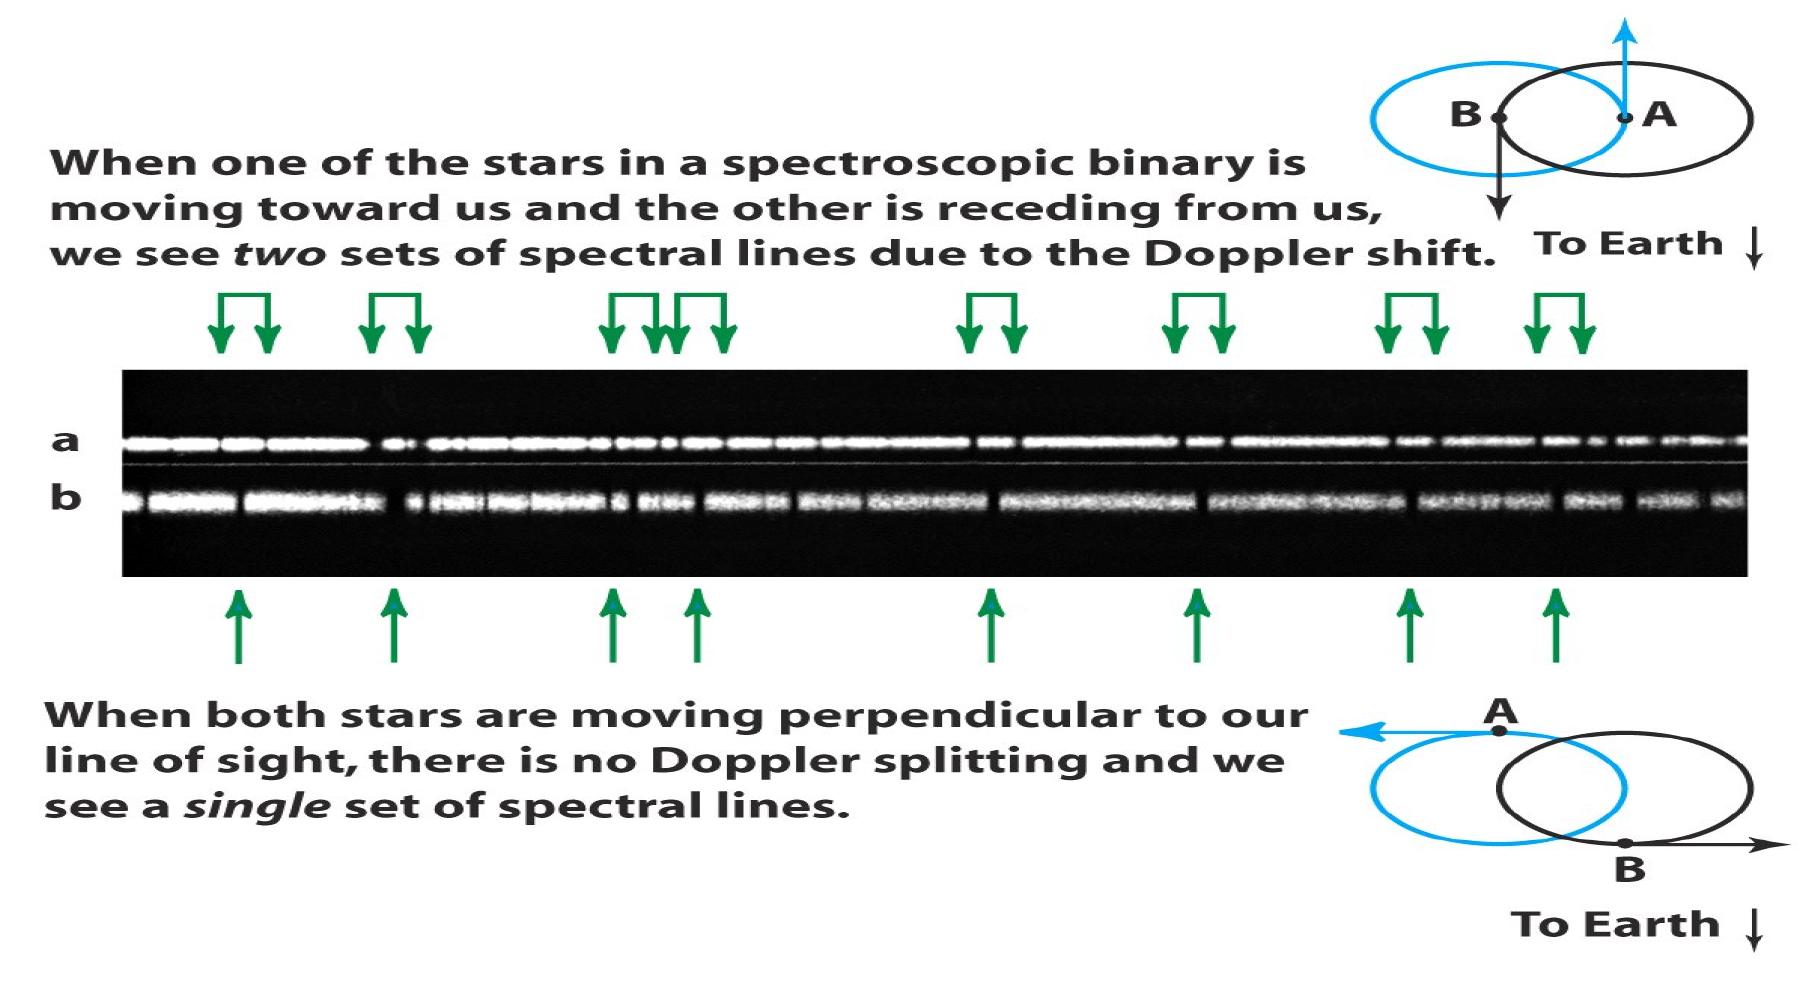
\includegraphics[width=\linewidth]{Figures/spectroscopic_binary.png}
            \caption{Φασματοσκοπικά διπλό σύστημα αστέρων.}
            \label{fig:spectroscopic_binary}
        \end{figure}
    Από το φάσμα που παίρνουμε, βλέπουμε ότι περιέχει γραμμές που ανήκουν σε δύο αστέρες (αν οι λαμπρότητες των μελών είναι συγκρίσιμες) ή μόνο σε έναν αστέρα (αν η λαμπρότητα του ενός είναι πολύ μεγαλύτερη από του άλλου). Κάθε φασματική γραμμή ``ταλαντώνεται'' περιοδικά γύρω από ένα μέσο μήκος κύματος. Προφανώς οι φασματικές γραμμές μετατοπίζονται προς το ερυθρό όταν ο αντίστοιχος αστέρας βρίσκεται στο τμήμα της τροχιάς που απομακρύνεται από τη Γη, και προς το κυανό όταν βρίσκεται στο τμήμα της τροχιάς που προσεγγίζει τη Γη (σχήμα \ref{fig:spectroscopic_binary}). Επειδή οι 2 αστέρες βρίσκονται πάντα σε αντιδιαμετρική θέση ως προς το ΚΜ, όταν οι φασματικές γραμμές του ενός αστέρα είναι μετατοπισμένες προς το ερυθρό, οι φασματικές γραμμές του άλλου είναι μετατοπισμένες προς το κυανό και αντίστροφρα. Οι περισσότεροι γνωστοί διπλοί αστέρες είναι φασματοσκοπικά διπλοί χωρίς αυτό να σημαίνει ότι δεν μπορούν να ανήκουν ταυτόχρονα και σε κάποια άλλη κατηγορία.
        
    Από τον χρόνο που χρειάζεται για να έχουμε δύο διαδοχικές ταυτήσεις των φασματικών γραμμών, μπορούμε να βρούμε την \textit{περίοδο} του συστήματος. Επίσης, ξέρουμε ότι η μετατόπιση από τη θέση ισορροπίας (της φασματικής γραμμής) εξαρτάται από τη συνιστώσα της \textit{ταχύτητας κατά μήκος της γραμμής παρατήρησης} (line of sight). Δεν έχουμε και τις 3 συνιστώσες για το διάνυσμα της ταχύτητας. Μέσω αυτής της συνιστώσας της ταχύτητας μπορούμε να βρούμε και την απόσταση των δύο σωμάτων μεταξύ τους (ανάλογα με το πως αλλάζει το πλάτος της ταχύτητας).
        
    \underline{Σημείωση}: Τα μήκη κύματος στα οποία εμφανίζονται οι μετατοπισμένες γραμμές απορρόφησης δεν αντιστοιχούν σε κανένα χημικό στοιχείο που μπορεί να δώσει μετάπτωση από μία ενεργειακή στιβάδα σε κάποια άλλη και να παράξει αυτά τα μήκη κύματος.
        
    Μέσω της μελέτης των φασματοσκοπικά διπλών αστέρων \textit{δεν} είναι δυνατόν να υπολογισθεί η μάζα των αστέρων του συστήματος, παρά μόνο ο λόγος των μαζών τους και το γινόμενο της κάθε μάζας επί την άγνωστη ποσότητα $\sin^3 i$, όπου $i$ είναι η γωνία κλίσης του επιπέδου της τροχιάς του διπλού συστήματος (σχήμα \ref{fig:inclination_angle}).
        \begin{figure}
            \centering
            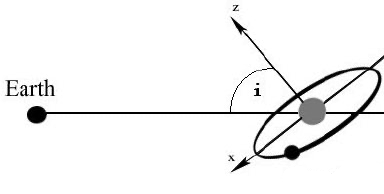
\includegraphics[scale=0.8]{Figures/inclination.jpg}
            \caption{Η γωνία κλίσης $i$, του επιπέδου της τροχιάς ενός διπλού συστήματος αστέρων.}
            \label{fig:inclination_angle}
        \end{figure}
        
    \item \textbf{Εκλειπτικά διπλοί αστέρες (ecliptic binaries)}\\
    Όταν το επίπεδο της τροχιάς των δύο αστέρων είναι σχεδόν παράλληλο με τη διεύθυνση παρατήρησης, δηλαδή η γωνία κλίσης $i \simeq 90^{\circ}$, και η απόσταση μεταξύ των μελών του συστήματος είναι πολύ μικρή, τότε κατά την περιφορά τους γύρω από το ΚΜ, τα 2 μέλη διέρχονται διαδοχικά το ένα μπροστά από το άλλο έτσι ώστε το ένα να καλύπτει τμήμα (ή και το σύνολο) του φαινόμενου δίσκου του άλλου, προκαλώντας μερικές ή όλικές εκλείψεις.
    Η ύπαρξη του ζεύγους συνεπάγεται από τις περιοδικές μεταβολές (αυξομειώσεις) της φαινόμενης λαμπρότητας του --φαινομενικά απλού-- αστέρα, η οποία μειώνεται κατά τη διάρκεια της έκλειψης.
    
    Κατά τη διάρκεια μίας περιφοράς συμβαίνουν δύο εκλείψεις, ανάλογα με το ποιό αστέρι βρίσκεται μπροστά από το άλλο και ως εκ τούτου παρουσιάζονται δύο ελάχιστα λαμπρότητας (σχήμα \ref{fig:eclipsing_binary}). Τα δύο αυτά ελάχιστα διαφέρουν γενικά ως προς το πλάτος και το βάθος, ανάλογα με τη λαμπρότητα των μελών του συστήματος.
        \begin{figure}[h]
            \centering
            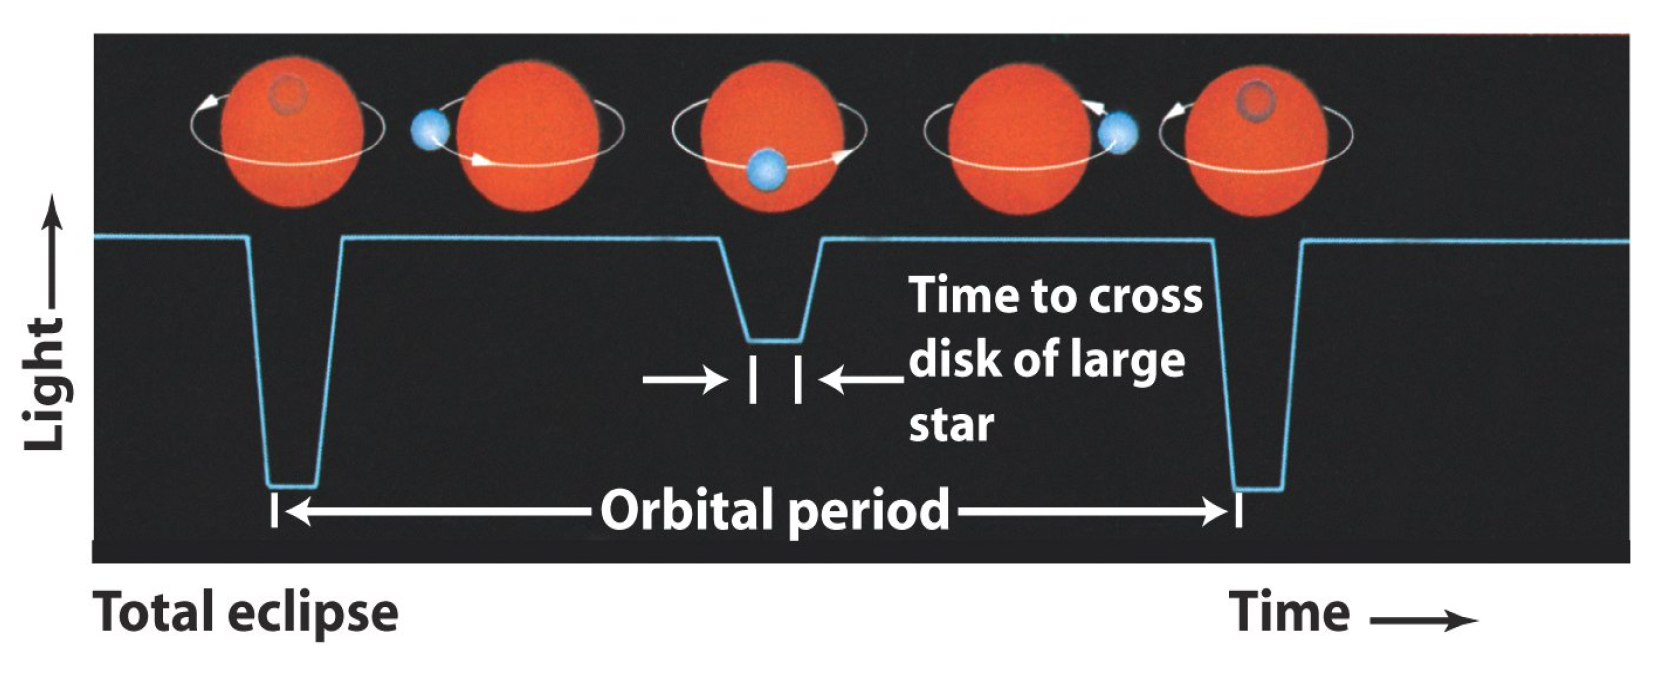
\includegraphics[width=\linewidth]{Figures/eclipsing_binary.png}
            \caption{Καμπύλη φωτός για ένα εκλειπτικά διπλό σύστημα αστέρων. Όταν ο αμυδρότερος αστέρας καλύπτει τον λαμπρότερο έχουμε το \textit{πρωτεύον ελάχιστο}. Στην αντίθετη περίπτωση έχουμε το \textit{δευτερεύων ελάχιστο}.}
            \label{fig:eclipsing_binary}
        \end{figure}
        
    Και σε αυτή την περίπτωση δεν μπορούμε να υπολογίσουμε τη μάζα κανενός από τους αστέρες του συστήματος. Από την καμπύλη φωτός όμως (σχήμα \ref{fig:eclipsing_binary}) μπορούμε να υπολογίσουμε την κλίση της τροχιάς, τις ακτίνες των μελών του ζεύγους και τον λόγο των φωτεινοτήτων των δύο αστέρων. Αν επιπροσθέτως τα δύο αστέρια ανήκουν στην κύρια ακολουθία μπορούμε να υπολογίσουμε και τον λόγο των μαζών από τη σχέση μάζας-φωτεινότητας.
    
    \item \textbf{Αστρομετρικά διπλοί αστέρες (astrometric binaries)}\\
    Στη κατηγορία αυτή κατατάσσονται τα μη-οπτικώς διπλά συστήματα αστεριών, των οποίων ο αμυδρός συνοδός αστέρας εντοπίζεται μόνο μέσω των δυναμικών επιδράσεων του πάνω στην τροχιά του πρωτεύοντος αστέρα. Ουσιαστικά παρατηρούμε μόνο ένα άστρο, επειδή όμως η κίνηση στην τροχιά του παρουσιάζει παλινδρομήσεις, συμπεραίνουμε ότι υπάρχει αμυδρός συνοδός.
    
    \item \textbf{Φασματικά διπλοί αστέρες (spectral binaries)}\\
    Αν οι τυπικές ταχύτητες περιφοράς των μελών ενός διπλού συστήματος ή/και η γωνία κλίσης $i$ είναι πολύ μικρή, τότε δεν είναι δυνατόν να ανιχνευθεί η μετατόπιση Doppler των φασματικών γραμμών και επομένως το σύστημα δεν αναγνωρίζεται ως φασματοσκοπικά διπλός αστέρας. Παρόλα αυτά, αν τα δύο μέλη έχουν σημαντικά διαφορετικά φάσματα (ανήκουν δηλαδή σε διαφορετικούς φασματικούς τύπους) και συγκρίσιμες λαμπρότητες (έτσι ώστε και τα δύο φάσματα να είναι ορατά), τότε το σύστημα μπορεί να αναγνωριστεί ως φασματικά διπλός αστέρας.
    
    Είναι φανερό ότι οι φασματικά διπλοί αστέρες διαφέρουν από τους φασματοσκοπικά διπλούς στο ότι στους πρώτους δεν παρατηρείται μετατόπιση Doppler των γραμμών. Κανένα στοιχείο δεν μπορεί να βρεθεί για τους φασματικά διπλούς αστέρες αφού δεν παρατηρούμε σ' αυτούς κανένα φαινόμενο που να εμφανίζει χρονική μεταβολή.
\end{enumerate}

\subsection{Βασικοί υπολογισμοί}

\subsubsection{Υπολογισμός στοιχείων τροχιάς}
Μετατρέποντας τη \textit{σχετική φαινόμενη τροχιά} σε \textit{σχετική πραγματική τροχιά}, υπολογίζουμε:
\begin{eqnarray*}
    \epsilon_{\pi} &=& \ \text{εκκεντρότητα} \\
    \alpha_{\pi} &=& \ \text{μεγάλος γωνιώδης ημιάξονας σε AU} \\
    i &=& \ \text{γωνία κλίσης}
\end{eqnarray*}

Αν γνωρίζουμε την παράλλαξη $\pi$, τότε υπολογίζουμε τον μεγάλο ημιάξονα $\alpha$ σε AU
\begin{equation}
    \alpha = \frac{\alpha_{\pi}}{\pi}
\end{equation}

\subsubsection{Υπολογισμός αθροίσματος μαζών}
Από τον 3ο νόμο του Kepler (σχέση \eqref{eq:Kepler_third_law}) έχουμε ότι 
$$M_1 + M_2 \simeq \frac{\alpha ^3}{P^2}$$ όπου $\alpha$ είναι ο μεγάλος ημιάξονας σε AU και $P$ η περίοδος του συστήματος.


\subsubsection{Υπολογισμός μαζών $M_1. M_2$}
Για φωτεινά διπλά συστήματα με σχετικά μεγάλη γωνιώδη απόσταση $\alpha_{\pi}$, μπορούμε να υπολογίσουμε και την \textit{απόλυτη φαινόμενη τροχιά} για καθένα από τα δύο μέλη. Άρα υπολογίζουμε δύο ημιάξονες $\alpha_1, \alpha_2$.

Από τον ορισμό του ΚΜ του συστήματος (σχέση \eqref{eq:center_mass}) και σε συνδυασμό με τον υπολογισμό του αθροίσματος $M_1 + M_2$ προκύπτουν οι μάζες $M_1, M_2$ για κάθε αστέρα.

\subsubsection{Δυναμικές παραλλάξεις}
 Από τις σχέσεις:
 \begin{eqnarray*}
    M_1 + M_2 &=& \frac{\alpha^3}{P^2} \\\\
    \alpha &=& \frac{\alpha_{\pi}}{\pi} 
 \end{eqnarray*}
 προκύπτει ότι:
 \begin{equation}
     \alpha_{\pi} = \pi \left[ (M_1 + M_2)P^2 \right]^{1/3}
 \end{equation}
 
 Αν οι δύο αστέρες ανήκουν στην κύρια ακολουθία, τότε για τον καθένα ισχύει ο νόμος μάζας-φωτεινότητας $L = f(M)$. Οπότε λύνουμε επαναληπτικά το σύστημα:
 
 \begin{eqnarray*}
    \pi &=& \alpha_{\pi} \left[ (M_1 + M_2)P^2 \right]^{-1/3} \\\\
    L_1 &=& f(M_1) \\\\
    L_2 &=& = f(M_2)
 \end{eqnarray*}
 για $\pi, M_1, M_2$ ξεκινώντας από κάποια εκτίμηση για το $M_1 + M_2$.  




\subsection{Στενά διπλά συστήματα \& απώλεια μάζας}
Κατά τη διάρκεια της ζωής τους, τα αστέρια χάνουν μάζα η οποία εμπλουτίζει τον μεσοαστρικό χώρο μέσω δύο διακασιών:
\begin{enumerate}[label=(\alph*)]
    \item \textbf{Συνεχώς}, μέσω των αστρικών ανέμων. Η μάζα που μπορεί να χαθεί με αυτόν τον τρόπο εξαρτάται από τη μάζα του αστέρα καθώς και το στάδιο της εξέλιξής του ($\dot{M}_{\text{Giant}} > \dot{M}_{MS}$).
    \item \textbf{Εκρηκτικώς}, μέσω καινοφανών και υπερκαινοφανών εκρήξεων.
\end{enumerate}

{\color{red} \hrule}
Στην περίπτωση ενός στενού διπλού συστήματος, οι αλληλεπιδράσεις μεταξύ των μελών μπορεί να οδηγήσει σε μεταφορά μάζας από το ένα αστέρι στο άλλο, επηρεάζοντας με αυτόν τον τρόπο την δομή, την μάζα, την γωνιακή στροφορμή καθώς και την τελική κατάσταση των αστέρων του συστήματος.
{\color{red} \hrule}

Όταν έχουμε ένα διπλό σύστημα, το πρόβλημα των πολλών σωμάτων (n-body problem) εκφυλίζεται στο ``περιορισμένο κυκλικό πρόβλημα των τριών σωμάτων'' (circular restricted three-body problem), με το ενεργό (effective) δυναμικό να δίνεται από τη σχέση:
\begin{equation}
    \label{eq:effective_potential}
    \Phi = - G \left( \frac{M_1}{r_1} + \frac{M_2}{r_2} \right) - \frac{1}{2} \Omega^2 r_3^2
\end{equation}
όπου  $r_1, r_2$ είναι οι αποστάσεις από το κέντρο των αστέρων $M_1, M_2$ αντίστοιχα, $\Omega$ είναι η τροχιακή γωνιακή ταχύτητα και $r_3$ είναι η απόσταση του άξονα περιστροφής τους συστήματος.

Η ποσότητα $\displaystyle V_g = - G \left( \frac{M_1}{r_1} + \frac{M_2}{r_2} \right)$ είναι ουσιαστικά το βαρυτικό δυναμικό ενώ το $\displaystyle V_F = - \frac{1}{2} \Omega^2 r_3^2$ περιγράφει το ``δυναμικό'' της φυγόκεντρου δύναμης. 

Αν απαιτήσουμε η συνολική δύναμη που ασκείται σε ένα δοκιμαστικό σωματίδιο, $m$, να είναι μηδέν: $$\boldsymbol{F_t} = - \nabla \Phi = 0$$
τότε η εξίσωση \eqref{eq:effective_potential} δίνει πέντε λύσεις όπου η βαρυτική δύναμη εξισορροπεί την φυγόκεντρο δύναμη που προκαλείται από τη σχετική κίνηση των δύο αστέρων του ενός γύρω από τον άλλον. Τα σημεία για τα οποία ισχύει αυτό, δηλαδή τα σημεία τα οποία έχουν μηδενική στιγμιαία ταχύτητα ονομάζονται \textit{σημεία Lagrange}, ($L_n, n = 1, \dots, 5$). Άρα αν το δοκιμαστικό σωματίδιο τοποθετούνταν σε κάποιο από αυτά τα σημεία, θα διατηρούσε τη θέση του σε σχέση ως προς τα δύο αστέρια.

Το σύνολο των σημείων μηδενικής ταχύτητας συγκροτεί μία ομάδα κλειστών επιφανειών, τις οποίες ονομάζουμε \textit{επιφάνειες μηδενικής ταχύτητας} (zero velocity surfaces) και περνούν από τα σημεία Lagrange. Η τομή μιας τέτοιας επιφάνειας μηδενικής ταχύτητας (ή ισοδυναμική επιφάνεια καθώς περιλαμβάνει όλα τα σημεία του συστήματος που μοιράζονται την ίδια τιμή του δυναμικού $\Phi$) με κάποιο συγκεκριμένο επίπεδο ονομάζεται \textit{καμπύλη μηδενικής ταχύτητας} (zero velocity curve). Συνήθως σαν επίπεδο τομής επιλέγεται το επίπεδο της σχετικής τροχιάς των δύο αστέρων του συστήματος (σχήμα \ref{fig:eq_sur}).
\\
{\color{red} \hrule}
Οι επιφάνειες μηδενικής ταχύτητας είναι σημαντικές γιατί ορίζουν τα όρια (boundaries) των περιοχών από τις οποίες το δοκιμαστικό σωματίδιο είναι δυναμικά αποκλεισμένο. Με άλλα λόγια, κάθε αστέρας ελέγχει βαρυτικά μόνο έναν περιορισμένο χώρο που καθορίζεται από μία ισοδυναμική επιφάνεια.
{\color{red} \hrule}

\begin{figure}[h]
   \centering
\begin{subfigure}[h]{0.45\textwidth}
	\centering
   	 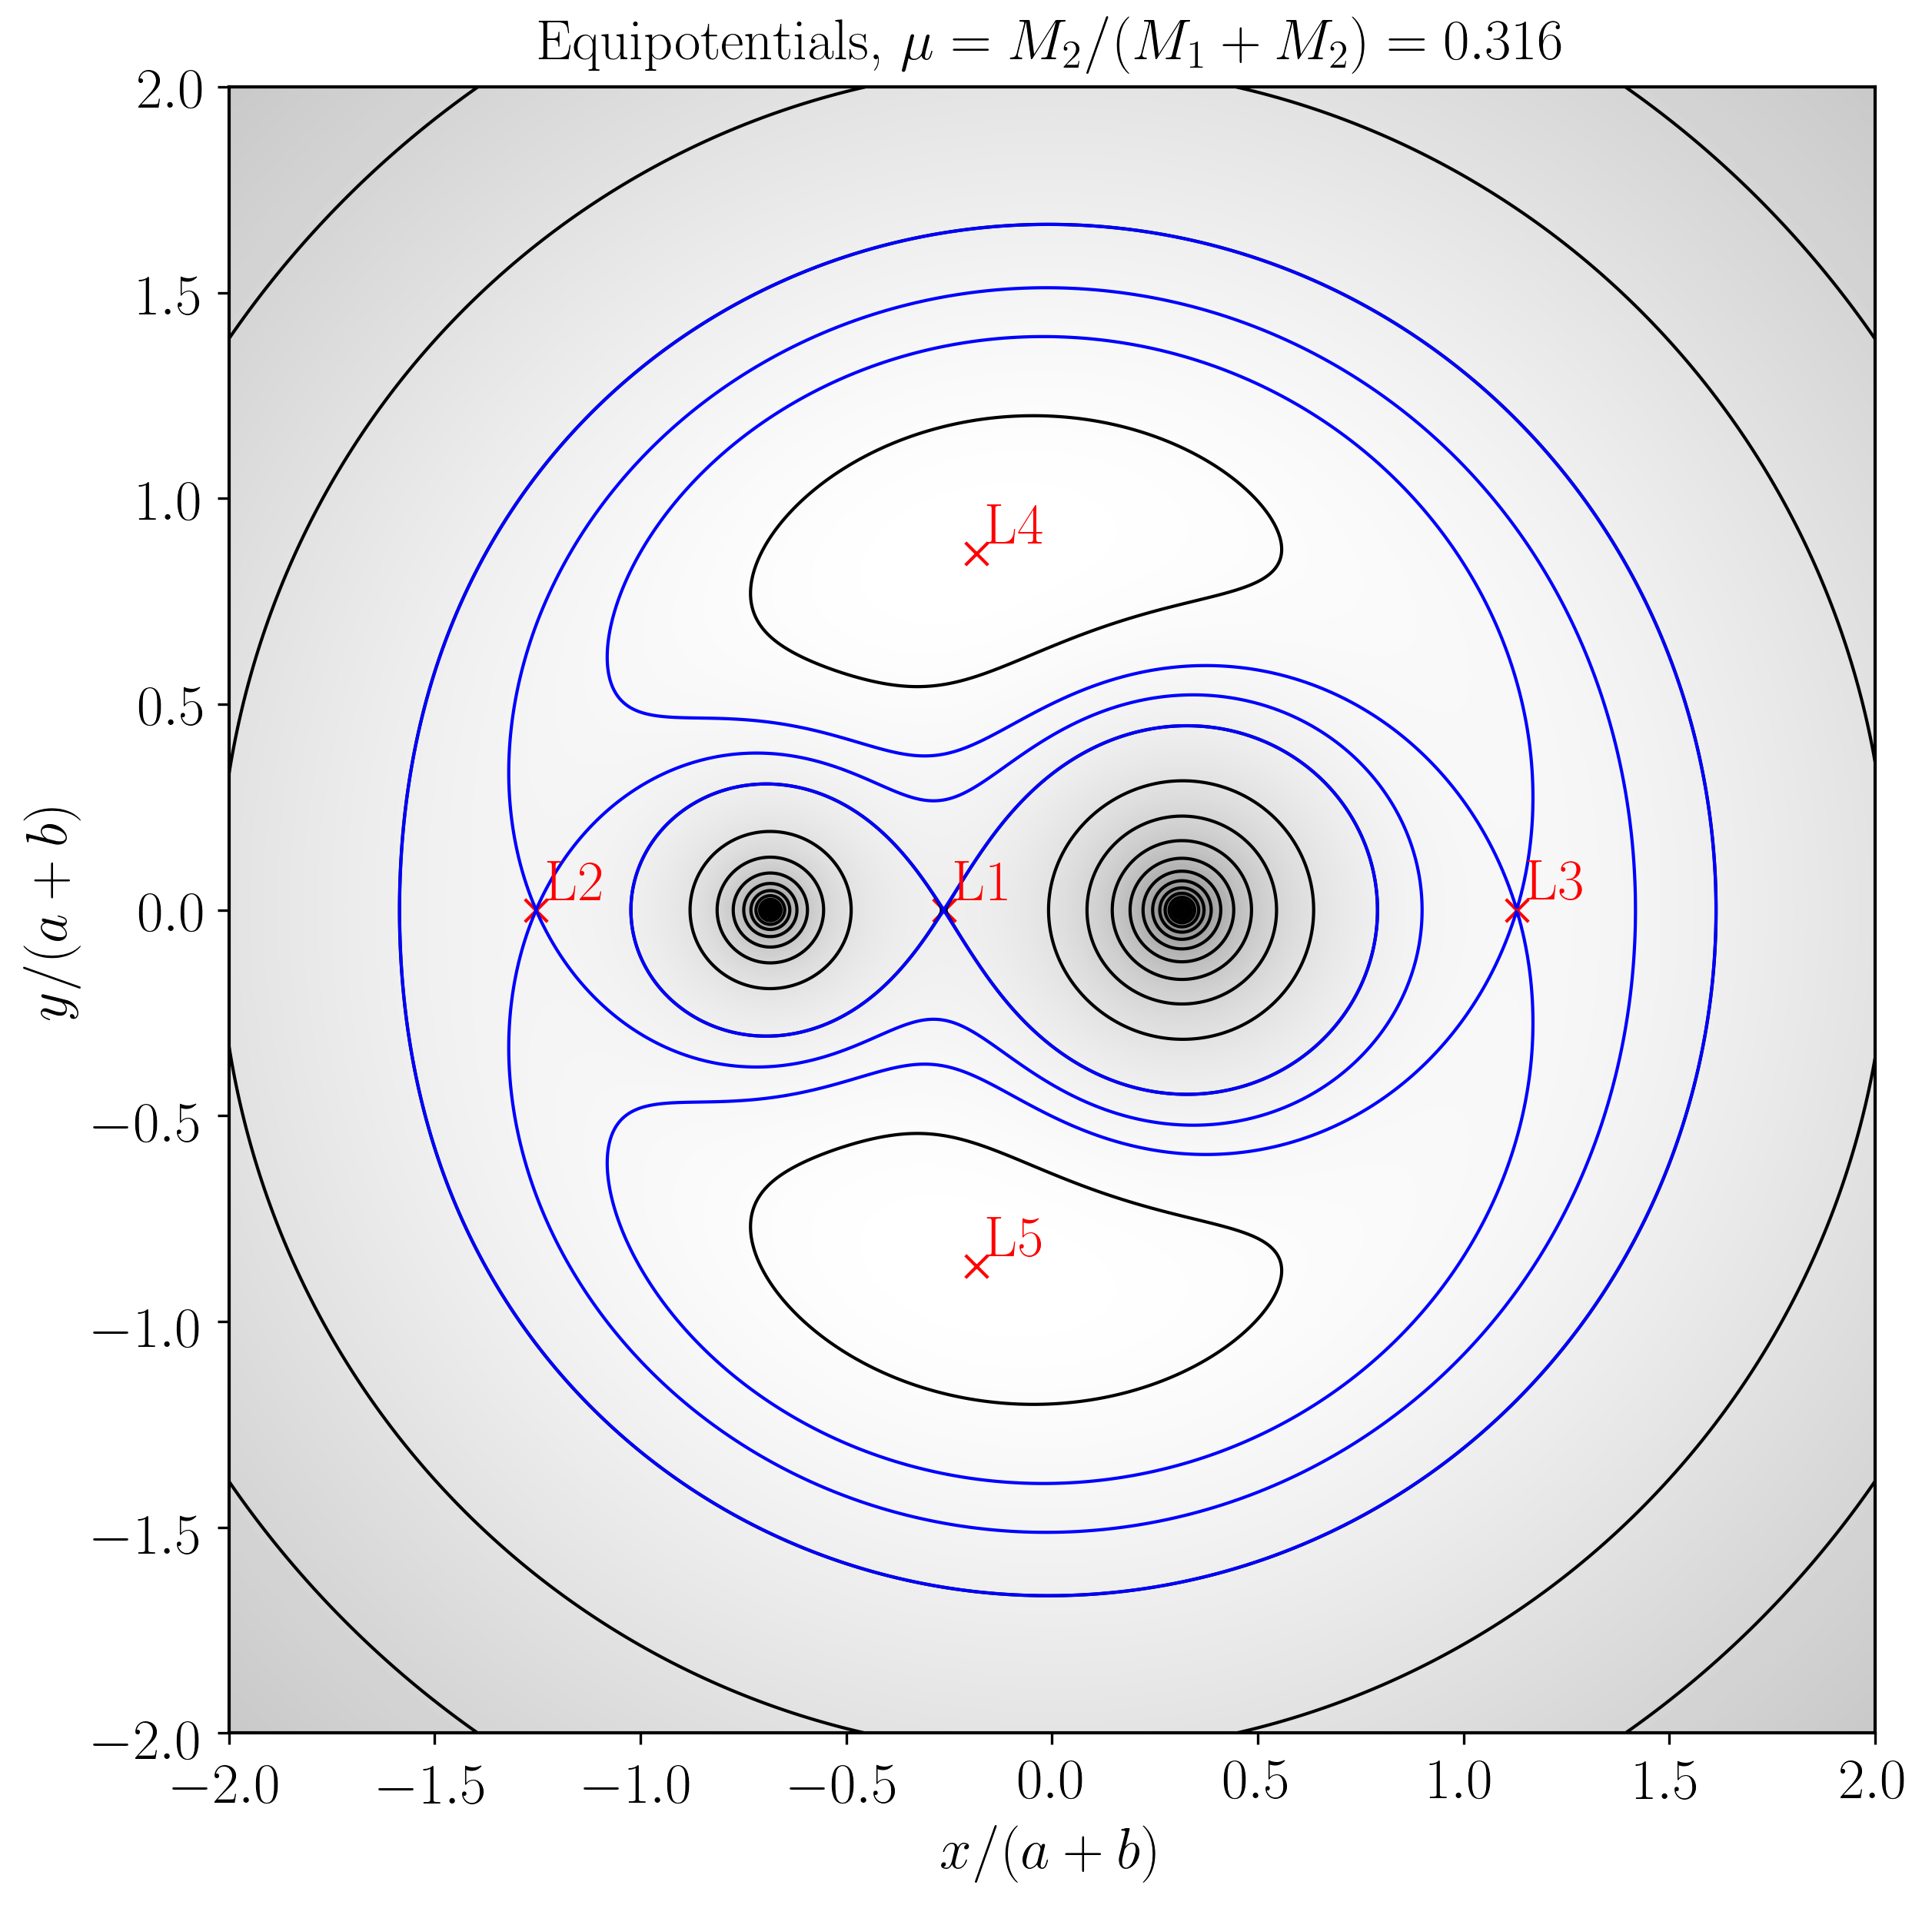
\includegraphics[width = \linewidth]{Figures/equipotentials_mu_0_316.png} 
\end{subfigure}
\begin{subfigure}[h]{0.535\textwidth}
	\centering
	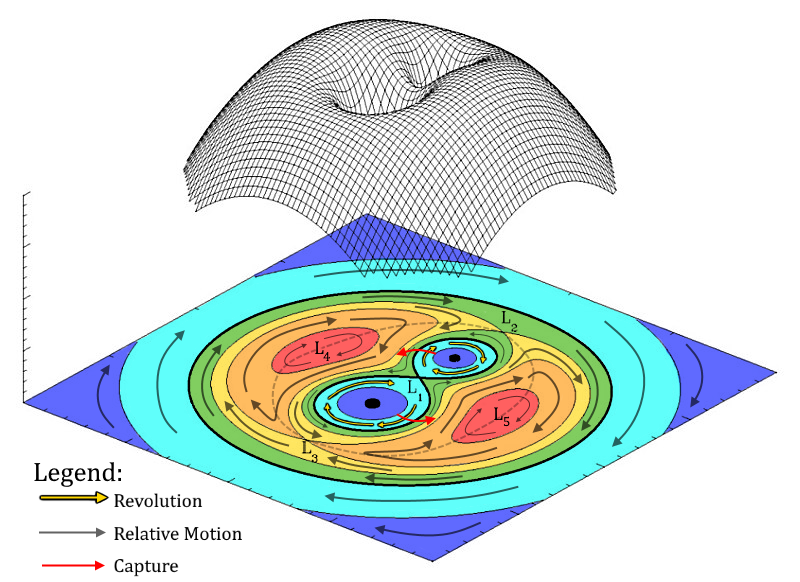
\includegraphics[width = \linewidth]{Figures/RochePotential_-_Colorized.png} 
    \end{subfigure}
    \caption{\textbf{Left panel}: Equipotential lines in the orbital plane of a rotating binary system, with a reduced mass ratio of $\mu = 0.316$. In this setup, $M_1$ is the more massive and is located at $x = +a$, whilst $M_2$ is the less massive and is at $x = -b$. The inner equipotential surface that passes from the $L_1$ Lagrangian point, defines the ``teardrop''-shaped Roche-lobes, one for each star. Contour lines passing through the Lagrange points are marked with blue colour. \textbf{Right Panel}: 3D representation of equipotential surfaces.}
    \label{fig:eq_sur}
\end{figure}

Στο σχήμα \ref{fig:eq_sur} κάθε καμπύλη μηδενικής ταχύτητας έχει παρουσιαστεί με διαφορετικό χρώμα. Από τα πέντε σημεία Lagrange, το $L_1$ παίζει σημαντικό ρόλο στην εξέλιξη των διπλών συστημάτων καθώς η ισοδυναμική επιφάνεια που περνάει από αυτό ορίζει τους (ανεξάρτητους μεταξύ τους) \textit{λοβούς Roche} και κάθε ένας από αυτούς περιβάλλει έναν αστέρα του συστήματος.

Η επιφάνεια μηδενικής ταχύτητας που περνάει από το $L_1$ έχει ένα ιδιαίτερο χαρακτηριστικό: όλες οι επιφάνειες μηδενικής ταχύτητας που περιβάλλουν ένα μόνο σώμα, βρίσκονται μέσα στον αντίστοιχο λοβό Roche, ενώ όλες οι επιφάνειες μηδενικής ταχύτητας που βρίσκονται έξω από τους λοβούς Roche περιβάλλουν και τα δύο σώματα. Έτσι, ένα δοκιμαστικό σωματίδιο που βρίσκεται μέσα στο λοβό Roche ενός μέλους του διπλού συστήματος ``ανήκει'' βαρυτικά σε αυτόν τον αστέρα. Αντίθετα, ένα σωματίδιο που βρίσκεται έξω και από τους δύο λοβούς Roche ``ανήκει'' βαρυτικά και στους δύο αστέρες, αφού κινείται σε τροχιά που είναι δυνατόν να περιβάλλει και τους δύο. Οι τροχιές αυτές δεν είναι κωνικές τομές (κύκλοι, ελλείψεις, παραβολές, υπερβολές ή ευθείες).

Με βάση το λόγο της ακτίνας του κάθε αστέρα ως προς την ακτίνα του δικού του λοβού ($R_L$), τα διπλά συστήματα χωρίζονται στις εξής κατηγορίες:

\subsubsection{Αποχωρισμένα (detached binaries)}
Είναι ένα διπλό σύστημα στο οποίο ο κάθε ένας αστέρας βρίσκεται εξ' ολοκλήρου μέσα στον δικό του λοβό Roche και εξελίσσονται σχεδόν ανεξάρτητα ο ένας από τον άλλον. Ισχύει δηλαδή ότι $r_1 < R_{L,1}$ και $r_2 < R_{L,2}$ όπου $r_1, r_2$ οι ακτίνες των δύο αστέρων.

\subsubsection{Ημιαποχωρισμένα (semidetached binaries)}
Αυτά είναι τα συστήματα στα οποία μόνο ο ένας από τους δύο αστέρες ``γεμίζει'' τον λοβό Roche του (δηλαδή $r_1 < R_{L,1}$ και $r_2 \approx R_{L,2}$). Αυτό μπορεί να συμβεί σε μετεγενέστερα εξελικτικά στάδια στη διάρκεια ζωής ενός αστέρα, όταν μπει στη φάση των γιγάντων,
Έκεί, η ακτίνα του μεγαλώνει σε τόσο βαθμό όπου ο όγκος του αστέρα είναι συγκρίσιμος με  τον όγκο που ορίζει ο λοβός Roche του.

Σε αυτή την περίπτωση έχουμε εκροή μάζας από αυτόν τον αστέρα προς τον συνοδό του διαμέσου το εσωτερικού $L_1$ σημείο Lagrange. Η προσαύξηση του υλικού γίνεται με τον σχηματισμό ενός \textit{δίσκου επισυσσώρευσησ/προσαύξησης} και όχι με το να πέφτει απευθείας πάνω στον συνοδό αστέρα. Αυτό συμβαίνει διότο το υλικό που εκρύεται έχει την ίδια στροφορμή με τον αστέρα-δότη και εκτός αν υπάρχουν μη-συντηρητικές μηχανισμοί για να αφαιρέσουν ένα ποσό από τη στροφορμή του αερίου που εκρύεται, αυτό θα συνεχιστεί να περιφέρεται γύρω από τον συνοδό αστέρα. Για να καταφέρει να πέσει πάνω στον αστέρα, η ύλη πρέπει να χάσει στροφορμή από την εσωτερική τριβή (ιξώδες). Αυτή η εσωτερική τριβή του αερίου το αναγκάζει να θερμανθεί και να ακτινοβολεί (X-ray binary).

Η υπερχείλιση του αστέρα μέσα από τον λοβό του Roche οδηγεί σε σημαντική μείωση της μάζας του αστέρα και επηρεάζει τη μετέπειτα εξέλιξή του. Πέρα από αυτόν τον μηχανισμό όμως, μπορούμε να έχουμε μεταφορά μάζας με προσαύξηση από τον \textit{αστρικό άνεμο} του θερμότερου αστέρα προς τον ψυχρότερο. Παρόλα αυτά, η μεταφορά μάζας με αυτόν τον τρόπο δεν είναι το ίδιο αποδοτική όσο η υπερχείλιση του λοβού Roche.

\subsubsection{Εν επαφή (contact binary)}
Ένα διπλό σύστημα λέμε ότι είναι σε επαφή ότα και τα δύο αστέρια ``γεμίζουν'' τους λοβούς τους (δηλαδή $r_1 \approx R_{L,1}$ και $r_2 \approx R_{L,2}$). Σε αυτή την περίπτωση, το σύστημα μοιράζεται μία κοινή ατμόσφαιρα (common envelope, σχήμα \ref{fig:binary_cases}) η οποία μπορεί να εκδιωχθεί στερώντας έτσι από το σύστημα ένα σημαντικό μέρος της μάζας του.

\begin{figure}
    \centering
    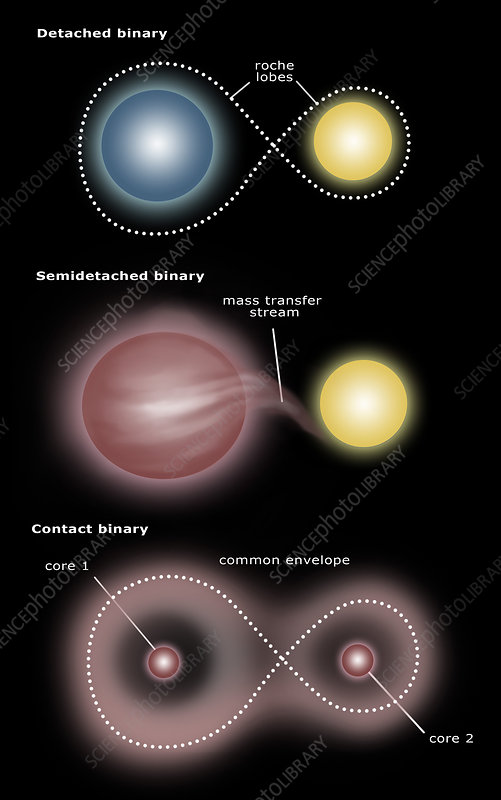
\includegraphics[scale=0.3]{Figures/binary_cases.jpeg}
    \caption{Κατηγορίες διπλών συστημάτων βάσει του ποσοστού πλήρωσης των λοβών Roche.}
    \label{fig:binary_cases}
\end{figure}

Σε αυτό το σημείονα διευκρινήσουμε ότι δεν υπάρχει αναλυτική έκφραση για το μέγεθος του λοβού Roche σε ένα διπλό σύστημα. Παρόλα αυτά έχει προταθεί μια αριθμητική προσέγγιση της ακτίνας του λοβού Roche μέσω της σχέσης:
$$\frac{R_L}{a} = \frac{0.49q^{2/3}}{0.6q^{2/3} + \ln (1 + q^{1/3})}$$
όπου $a$ είναι ο τροχιακός διαχωρισμός (orbital separation) του συστήματος και $\displaystyle q \equiv \frac{M_{\text{donor}}}{M_{\text{accretor}}}$ είναι ο λόγος των μαζών των μελών του συστήματος.
Αυτές είναι και οι δύο πιο σημαντικές παράμετροι για να ακολουθήσουμε την εξέλιξη του συστήματος.













\section{Μεταβλητοί αστέρες}
Μεταβλητοί αστέρες ονομάζονται οι αστέρες, των οποίων η λαμπρότητα μεταβάλλεται μέσα σε ένα χρονικό διάστημα σημαντικά μικρότερο από την ηλικία τους. Με τον (γενικά ασαφή) αυτό ορισμό αποφεύγει κανείς να χαρακτηρίσει μεταβλητούς όλους τους αστέρες, αφού, η λαμπρότητα ενός αστέρα μεταβάλλεται σημαντικά, και μάλιστα κατά πολλές τάξεις μεγέθους, στη διάρκεια της ζώης τους (π.χ. εγκατάσταση στην κύρια ακολουθία, άνοδος στον κλάδο των γιγάντων κτλ.)

Οι μεταβλητοί αστέρες κατατάσσονται σε κατηγορίες, ανάλογα με το φαινόμενο που προκαλεί τη μεταβολή της λαμπρότητά τους, την περιοδικότητα (ή την έλλειψη αυτής) της μεταβολής και το μέγεθός της. Καταρχάς, οι μεταβλητοί αστέρες μπορούν να χωριστούν σε γνήσιους μεταβλητούς και σε μη-γνήσιους. Στην τελευταία περίπτωση, η μεταβολή της λαμπρότητας του αστέρα δεν οφείλεται σε κάποιον ενδογενή φυσικό μηχανισμό αλλά σε κάποιον εξωτερικό παράγοντα που επηρεάζει φαινομενικά την λαμπρότητα. 

Η απλούστερη περίπτωση ενός τέτοιου μη-γνήσιου μεταβλήτού αστέρα είναι εκείνη, κατά την οποία ο αστέρας είναι στην πραγματικότητα εκλειπτικά διπλός και η μεταβολή της λαμπρότητάς του οφείλεται στο γεγονός ότι, κατά την κίνησή τους, τα μέλη του διέρχονται διαδοχικά το ένα μπροστά από το άλλο, προκαλώντας εκλείψεις. Η διάρκεια των εκλείψεων, ο ρυθμός ελλάτωσης και αύξησης της λαμπρότητας του διπλού αστέρα κατά την αρχή και το τέλος των εκλείψεων, η αλλαγή του δείκτη χρώματος και η περίοδος του φαινομένου δίνουν πληροφορίες για την απόσταση μεταξύ των μελών, τη μάζα τους, τις διαστάσεις τους, το φασματικό τους τύπο κτλ.
Από την άλλη μεριά, οι γνήσιοι μεταβλητοί αστέρες χωρίζονται στις κατηγορίες που θα αναλύσουμε παρακάτω.

\subsection{Περιοδικοί}
\subsubsection{Κηφείδες}
Οι Κηφείδες αστέρες αποτελούν τη σημαντικότερη κατηγορία περιοδικών μεταβλητών αστέρων. Ονομάστηκαν έτσι καθώς ο πρώτος τέτοιος αστέρας που μελετήθηκε ήταν ο ``δ Κηφέως'' στον αστερισμό του Κηφέα. Οι Κηφείδες είναι γίγαντες αστέρες και παρουσιάζουν περιοδικές μεταβολές στη λαμπρότητά τους, με περίοδο από 1 εως 50 ημέρες. Κατά τη διάρκεια μιας περιόδου, εκτός από την λαμπρότητα του αστέρα, που μεταβάλλεται κατά $\Delta m \simeq 1$ μέγεθος, μεταβάλλονται επίσης και ο δείκτης χρώματός του, και επομένος ο φασματικός του τύπος (και άρα η επιφανειακή του θερμοκρασία). Συνέπεια του γεγονότος αυτού είναι ότι η θέση των αστέρων αυτών δεν μένει σταθερή στο διάγραμμα H-R αλλά μετατοπίζεται, εκτελώντας μία κλειστή τροχιά κατά τη διάρκεια μιας περιόδου.

Η μεταβολή της λαμπρότητας των Κηφείδων δεν οφείλεται μόνο στη μεταβολή της θερμοκρασίας των αστέρων αυτών, αλλά και σε μεταβολή της ακτίνας τους. Επομένως οι αστέρες αυτοί παρουσιάζουν \textbf{αναπάλσεις} (pulsations). Αυτές οι αναπάλσεις αφορούν τα εξωτερικά στρώματα του αστέρα και δεν οφείλονται σε μεταβολές του ρυθμού παραγωγής ενέργειας στον πυρήνα καθώς τέτοια φαινόμενα θα εξελίσσονταν στην θερμική χρονική κλίμακα που είναι της τάξης των δεκάδων χιλιάδων ετών. Γίνεται φανερό ότι οι Κηφείδες δεν είναι γεννημένοι μεταβλητοί, αλλά αποτελούν μία φάση στην εξέλιξη ορισμένων αστέρων, μετά την έξοδό τους από την κύρια ακολουθία.

Αποδεικνύεται ότι για τους Κηφείδες αστέρες ισχύει μία σχέση μεταξύ της περιόδου και της λαμπρότητας της μορφής
\begin{equation}
    \label{eq:cepheids_period_luminosity_relation}
    \log P = \alpha \log L + \beta 
\end{equation}
όπου $\alpha$ και $\beta$ είναι αριθμητικές σταθερές. Μερικές φορές αυτή η σχέση εκφράζεται και με όρους απόλυτου μεγέθους αντί λαμπρότητας. Σε συνδυασμό με τη παρατηρούμενη μεταβολή στο φαινόμενο μέγεθος των Κηφείδων, η σχέση \eqref{eq:cepheids_period_luminosity_relation} μπορεί να χρησιμοποιηθεί για την εκτίμηση της απόστασης μέσω του distance modulus. Μέχρι σήμερα, έχουν μετρηθεί οι αποστάσεις πολλών γαλαξιών που φιλοξενούν Κηφείδες αστέρες χρησιμοποιώντας αυτή την μέθοδο.

\subsubsection{RR Lyrae}
Οι αστέρες αυτοί είναι μεταβλητοί μικρής περιόδου, η μεταβολή της φωτεινότητας των οποίων οφείλεται επίσης σε σφαιρικα συμμετρικές (ακτινικές) αναπάλσεις. Είναι κιτρινόλευκοι γίγαντες αστέρες (οριζόντιος κλάδος στο διάγραμμα H-R) ενώ έχουν μάζα και περίοδο μικρότερες από αυτές των Κηφείδων ($M \simeq 0.5\,M_\odot$, $P \sim 0.2 - 1\,\text{ημέρα}$). Η λαμπρότητά τους είναι σχεδόν ανεξάρτητη της περιόδου αναπάλσεως και αντιστοιχεί σε απόλυτο μέγεθος $M_V = 0.6$. Οι αστέρες αυτοί, πάντως, είναι αμυδρότεροι από τους Κηφείδες, και έτσι δεν είναι ορατοί σε μεγάλες αποστάσεις. Επομένως είναι χρήσιμοι για μετρήσεις αποστάσεων μέσα στο Γαλαξία, αλλά όχι για μετρήσεις αποστάσεων άλλων γαλαξιών.

\subsubsection{Μακροπερίοδοι}
Κατά τα τελευταία στάδια της εξέλιξης αστέρων μικρών μάζας είναι δυνατόν να υπάρξει συντονισμός των εξωτερικών στρωμάτων ενός αστέρα με το ρυθμό παραγωγής ενέργειας κατά τις διαδοχικές εναλλαγές καύσης των φλοιών H και He. Ο αστέρας τότε παρατηρείται ως μακροπερίοδος \textbf{μεταβλητός τύπου Mira} (Mira variable) με περίοδο, $P$, μεταξύ 100 και 1000 ημερών και εύρος μεταβολής μεγέθους $\Delta m_V \simeq 2 - 6\,\text{μεγέθη}$.

Οι μεταβλητοί τύπου Mira είναι ψυχροί, ερυθροί γίγαντες αστέρες μικρής μάζας και φασματικού τύπου Μ. Στο φάσμα τους παρατηρούνται ιδιαίτερα ισχυρές μοριακές γραμμές απορρόφησης. Το μεγάλο εύρος της μεταβολής του μεγέθους αυτών των αστέρων μπορεί να εξηγηθεί από το γεγονός ότι ο συντελεστής απορρόφησης εξαρτάταται ισχυρά από τη θερμοκρασία.

\subsection{Μη-περιοδικοί}
\subsubsection{Ανώμαλοι - T Tauri}
Οι αστέρες αυτοί πήραν το όνομά τους από τον τυπικό εκπρόσωπό της κατηγορίας, το μεταβλητό αστέρα Τ στον αστερισμό του Ταύρου. Παρατηρησιακά οι αστέρες αυτοί χαρακτηρίζονται:
\begin{enumerate}
    \item από απότομες και βραχυχρόνιες αυξήσεις της φωτεινότητάς τους από λίγα δέκατα του μεγέθους μέχρι και 4 μεγέθη, τις οποίες διαδέχονται διαστήματα ηρεμίας που διαρκούν από λίγες ώρες μέχρι και 100 ημέρες,
    \item από φασματικές γραμμές λιθίου (οι οποίες δεν εμφανίζονται σε άλλους αστέρες καθώς το λίθιο εξαντλείται πολύ γρήγορα κατά την έναρξη των θερμοπυρηνικών αντιδράσεων στους αστέρες) και
    \item από ισχυρούς αστρικούς ανέμους.
\end{enumerate}
Από την ερυθρή χρώση του φωτός τους και από το φάσμα τους βρίσκουμε ότι περιβάλλονται από ένα νέφος αερίου και σκόνης και ότι η θέση τους στο διάγραμμα H-R είναι μεταξύ των ερυθρών γιγάντων και της κύριας ακολουθίας. Η παρουσία λιθίου και η θέση τους στο διάγραμμα H-R μας κάνουν να πιστεύουμε ότι οι αστέρες της κατηγορίας αυτής είναι αστέρες ``εν τη γενέσει τους'', δηλαδή αστέρες που βρίσκονται ακόμα στο τελευταίο στάδιο της βαρυτικής συστολής τους. Επομένως οι αστέρες αυτοί δεν έχουν φτάσει ακόμα στη κύρια ακολουθία.

\subsubsection{Ανώμαλοι - Αστέρες εκλάμψεων}
Οι αστέρες αυτοί είναι ψυχροί ερυθροί νάνοι της κύριας ακολουθίας, οι οποίοι παρουσιάζουν σε ακανόνιστα χρονικά διαστήματα απότομες και σύντομες αυξήσεις της φωτεινότητάς τους (κυρίως στα χρώματα B και U αλλά και στα ραδιοφωνικά μήκη κύματος) μέχρι και 6 μεγέθη, γνωστές ως \textbf{εκλάμψεις} (flares). Σήμερα πιστεύουμε ότι οι εκλάμψεις αυτών των αστέρων είναι της ίδιας φύσης με τις ηλιακές, οφείλονται δηλαδή σε απελευθέρωση μαγνητικής ενέργειας από επανασύνδεση μαγνητικών γραμμών (magnetic reconnection).

Η ενέργεια μιας τυπικής τέτοιας έκλαμψης είναι πολλές τάξεις μεγέθους μεγαλύτερη από την ενέργεια μιας τυπικής ηλιακής έκλαμψης. Η διαφορά αυτή αποδίδεται στο γεγονός ότι το μαγνητικό πεδίο των αστέρων εκλάμψεων είναι κατά πολύ ισχυρότερου του ηλιακού, επειδή η ζώνη μεταφοράς, στην ύπαρξη της οποίας οφείλεται το μαγνητικό πεδίο (σύμφωνα με τη θεωρία της μαγνητικής γεννήτριας του Parker), είναι πολύ μεγαλύτερη στους αστέρες εκλάμψεων. Πραγματικά, σήμερα πιστεύουμε ότι οι νάνοι της κύριας ακολουθίας φασματιών τύπων Μ3 - Μ9 δεν έχουν καθόλου ζώνη ακτινοβολίας, έτσι ώστε η ζώνη μεταφοράς καλύπτει όλο το εσωτερικό του αστέρα, εκτός από τον πυρήνα του.

\subsubsection{Ανώμαλοι - R Coronae Borealis}
Οι υπεργίγαντες αυτοί αστέρες φασματικού τύπου F χαρακτηρίζονται ως ``αντίστροφοι καινοφανείς'', διότι η φωτεινότητά τους ελλατώνεται ενίοτε κατά πολλά (έως και 9) μεγέθη μέσα σε πολύ μικρό χρονικό διάστημα (λίγες ημέρες), παραμένει χαμηλή για λίγο και στη συνέχεια επανέρχεται στην αρχική της τιμή. Γενικά το φάσμα τους είναι φτωχό σε γραμμές υδρογόνου και πλούσιο σε γραμμές άνθρακα. Η ασυνήθιστη αυτή χημική σύσταση οφείλεται είτε στη μεταφορά ύλης από τον πυρήνα προς τη φωτόσφαιρά τους (dredge up), είτε διότι κατά το στάδιο του γίγαντα έχασαν τους φλοιούς H και He που περιέβαλλαν τον πυρήνα.

Σύμφωνα με το πιο διαδεμένο πρότυπο, οι μεταβλητοί τύπου \textbf{R Coronae Borealis} (δηλαδή όμοιοι με τον μεταβλητό αστέρα R του αστερισμού του Βόρειου Στέφανου, R CBr) έχουν πολύ ισχυρούς αστρικούς ανέμους, με τους οποίους ο χώρος γύρω τους εμπλουτίζεται με ενώσεις άνθρακα. 'Οταν οι ενώσεις αυτές ψυχθούν, σχηματίζονται κόκκοι ανθρακούχου σκόνης οι οποίοι απορροφούν έντονα σε όλα τα μήκη κύματος. Σε αυτήν ακριβώς την απορρόφηση οφείλονται τα ελάχιστα της φωτεινότητας που παρατηρούμε. Η απορρόφηση όμως της ακτινοβολίας του αστέρα ανεβάζει τη θερμοκρασία των κόκκων της σκόνης, με αποτέλεσμα αυτοί να εξαχνωθούν και να επανέλθει ο αστέρας στην αρχική του φωτεινότητα.

\subsubsection{Καταστροφικοί - Γενικά στοιχεία}
Στους καταστροφικούς μεταβλητούς ανήκουν οι \textbf{καινοφανείς} (novae) και \textbf{υπερκαινοφανείς} (supernovae) αστέρες, κύριο χαρακτηριστικό των οποίων είναι η απότομη (σε διάστημα ωρών ως ημερών) και μεγάλη (πάνω από 4 και συχνά πάνω απο 10 μεγέθη) αύξηση της λαμπρότητάς τους. Η κατάταξη αυτών των αστέρων βασίζεται σε παρατηρησιακά κριτήρια και δεν αντανακλά απαραίτητα τους φυσικούς μηχανισμούς που προκαλούν τις τεράστιες αυτές αναλάμψεις. Αποτέλεσμα του γεγονότος αυτού είναι ότι αναλάμψεις που οφείλονται σε διαφορετικούς μηχανισμούς μπορεί να καταταγούν στην ίδια κατηγορία, ενώ αναλάμψεις που οφείλονται σε παρόμοιο μηχανισμό μπορεί να καταλήξουν σε διαφορετικές κατηγορίες.

Η απαίτηση που έχουμε από μια θεωρία για τη δημιουργία των καινοφανών και υπερκαινοφανών είναι να εξηγεί, τουλάχιστον, τη μορφή της καμπύλης φωτός (light curve) του αστέρα, δηλαδή να εξηγεί τον χρόνο ανόδου, τη μέγιστη λαμπρότητα, και το ρυθμό καθόδου, καθώς επίσης και το παρατηρούμενο φάσμα. Οι θεωρίες που έχουν προταθεί για την ερμηνεία των καινοφανών και υπερκαινοφανών μπορούν να καταταγούν σε δύο γενικές κατηγορίες:
\begin{enumerate}
    \item σε αυτές που αναφέρονται στην εξέλιξη \textbf{μεμονωμένων} αστέρων μεγάλης μάζας και
    \item σε αυτές που αναφέρονται στην εξέλιξη \textbf{διπλών συστημάτων} μέτριας μάζας.
\end{enumerate}
Σήμερα πιστεύουμε ότι οι υπερκαινοφανείς τύπου II ακολουθούν το πρώτο σενάριο, ενώ οι υπερκαινοφανείς τύπου I και οι καινοφανείς το δεύτερο σενάριο.

\begin{figure}
    \centering
    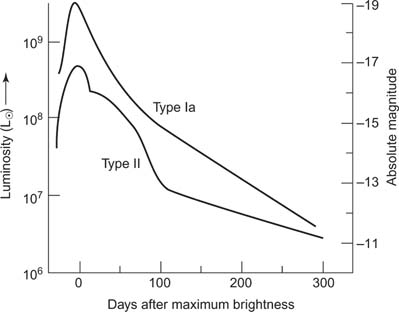
\includegraphics{Figures/sne_light_curves.jpeg}
    \caption{Καμπύλες φωτός υπερκαινοφανών αστέρων}
    \label{fig:sne_light_curves}
\end{figure}

\subsubsection{Καταστροφικοί - Καινοφανείς}
Σύμφωνα με το γενικά παραδεκτό σήμερα σενάριο, οι καινοφανείς αστέρες προέρχονται από την εξέλιξη διπλών συστημάτων. Σε ένα διπλό σύστημα με δύο αστέρες 1 και 2, που έχουν μάζες $M_1 > M_2$, ο αστέρας 1 εγκαταλείπει πρώτος την κύρια ακολουθία και αρχίζει να εξελίσσεται σε ερυθρό γίγαντα. Αν η απόσταση των δύο αστέρων ειναι αρκετά μικρή, τότε ο αστέρας 1 γεμίζει τον δικό του λοβό Roche, και μάζα από τα εξωτερικά του στρώματα μεταφέρεται στον αστέρα 2. 'Οταν τελειώσει αυτή η διαδικασία, τότε από τον αστέρα 1 δεν έχει απομείνει παρά μόνο ο πυρήνας του, ο οποίος τελικά καταλήγει (αν η μάζα του δεν υπερβαίνει το όριο Chandrasekhar) σε λευκό νάνο μάζας $M \sim 1\,M_\odot$. Παράλληλα ο αστέρας 2 έχει γίνει ήδη πολύ μεγαλύτερος (λόγω της προσαύξησης μάζας από τον αστέρα 1) και αρχίζει να εξελίσσεται με τη σειρά του σε ερυθρό γίγαντα. Κατά την εξέλιξη αυτή γεμίζει με τη σειρά του τον δικό του λοβό Roche, και αρχίζει πλέον η αντίστροφη μεταφορά μάζας από τον αστέρα 2 στον αστέρα 1 (λευκό νάνο).

'Οταν η μάζα της ύλης που συσσωρεύεται στη θερμή ατμόσφαιρα του λευκού νάνου ξεπεράσει κάποια κρίσιμη τιμή, τότε η πίεση και η θερμοκρασία στη βάση της ατμόσφαιράς του επιτρέπουν τη καύση του υδρογόνου σε ήλιο, αντίδραση που συμβαίνει σχεδόν ακαριαία. Η ενέργεια που εκλύεται από την έναρξη της θερμοπυρηνικής αυτής αντίδρασης απελευθερώνεται με τη μορφή μιας μεγάλης έκρηξης, που μπορεί να ανεβάσει τη λαμπρότητα του συστήματος κατά 10 μεγέθη, σε διάστημα μερικών ωρών.

Εφόσον η ροή ύλης από τον αστέρα 2 στον αστέρα 1 συνεχίζεται, μια τέτοια έκρηξη θα επαναλαμβάνεται κάθε φορά που η συσσωρευμένη μάζα ξεπερνά την κρίσιμη τιμή. Αν ο ρυθμός μεταφοράς είναι μεγάλος, τότε το πρότυπο αυτό προβλέπει ότι η κρίσιμη τιμή της μάζας είναι μικρή, επειδή η ύλη δεν προλαβαίνει να ``απλωθεί'' σε μεγάλη έκταση. Στην περίπτωση αυτή οι εκρήξεις αυτές επαναλαμβάνονται σε σύντομα χρονικά διαστήματα, αλλά είναι μικρές. Αντίθετα, αν ο ρυθμός μεταφοράς είναι μικρός, τότε οι εκρήξεις απέχουν χρονικά πολύ μεταξύ τους, αλλά είναι μεγάλες.

Σύμφωνα με το παραπάνω σενάριο, όλοι οι καινοφανείς πρέπει να είναι α) διπλοί και β) επαναληπτικοί. Τα μέχρι τώρα παρατηρησιακά δεδομένα υποστηρίζουν ικανοποιητικά την παραπάνω θεωρία σχηματισμού των υπερκαινοφανών. Ας σημειωθεί όμως ότι υπάρχουν και θεωρίες για την προέλευση των υπερκαινοφανών εκρήξεων που βασίζονται στην εξέλιξη απλών (μεμονωμένων) αστέρων, και δεν αποκλείεται μερικοί από τους καινοφανείς που παρατηρούμε να οφείλεται σε τέτοιες περιπτώσεις.

\subsubsection{Καταστροφικοί - Υπερκαινοφανείς I}
Για τους υπερκαινοφανείς τύπου I δεν υπάρχει σήμερα μια θεωρία τόσο γενικά παραδεκτή, όσο για τους υπερκαινοφανείς τύπου II ή τους καινοφανείς. Το πιο δημοφιλές σενάριο είναι παρόμοιο με αυτό των καινοφανών. Υπάρχει δηλαδή ένα διπλό σύστημα, το ένα μέλος του οποίου είναι ένας λευκός νάνος άνθρακα-οξυγόνου. Μάζα μεταφέρεται από τον συνοδό αστέρα στον λευκό νάνο και, έτσι, η μάζα του τελευταίου συνεχώς αυξάνει χωρίς την παρουσία εκρηκτικών αναλάμψεων αυτή το φορά. 'Οταν η μάζα του λευκού νάνου πλησιάζει το όριο Chandrasekhar, προκαλειται ανάφλεξη του άνθρακα στο εσωτερικό του λευκού νάνου και η παραγόμενη ενέργεια  θερμαίνει και εκτινάσσει τα ανώτερα στρώματα του αστέρα στο διάστημα. Η έκρηξη αυτή που ονομάζεται υπερκαινοφανής τύπου I είναι τόσο σφοδρή ώστε διαλύει το σύστημα και δεν αφήνει πίσω κάποιο συμπαγές αστρικό αντικείμενο, όπως π.χ. έναν αστέρα νετρονίων.

Το γεγονός ότι η έκρηξη συμβαίνει πάντα κοντά στην ίδια τιμή μάζας (όριο Chandrasekhar) σημαίνει ότι η ενέργεια από μία τέτοια έκρηξη (συγκεκριμένα από υπερκαινοφανείς τύπου Ia) είναι γνωστή (της τάξης των $10^{51}\,\text{erg}$). Αυτό μας επιτρέπει να χρησιμοποιήσουμε αυτές τις εκρήξεις ως ``σταθερά κεριά'' (standard candles) των οποίων γνωρίζουμε την λαμπρότητα, και άρα μπορούμε να τα χρησιμοποιήσουμε ως δείκτες για την μέτρηση αποστάσεων.


\subsubsection{Καταστροφικοί - Υπερκαινοφανείς II}
Σύμφωνα με την επικρατούσα σήμερα άποψη, η κατάληξη ενός αστέρα μεγάλης μάζας ($M > 5\,M_\odot$) είναι ένας υπερκαινοφανής τύπου II. Για αστέρες με μάζα στο διάστημα $5 < M/M_\odot < 10$ ο μηχανισμός του φαινομένου οφείλεται στην \textbf{έκρηξη άνθρακα} (carbon detonation) η οποία είναι παρόμοια με την λάμψη ηλίου που έχουμε περιγράψει αλλά πολύ πιο βίαιη. Για αστέρες με μάζα $M > 10\,M_\odot$ ο μηχανισμός του φαινομένου οφείλεται στην καταστροφική κατάρρευση ενός αδρανούς πυρήνα σιδήρου.

'Ενας αστέρας που έχει εξαντλήσει όλα τα πυρηνικά του καύσιμα (έχει δηλαδή δημιουργήσει έναν πυρήνα από σίδηρο), αρχίζει να καταρρέει, αφού δεν υπάρχει εσωτερική πηγή πίεσης που να αντισταθμίζει το βάρος των υπερκείμενων στρωμάτων. Επειδή η μάζα του πυρήνα είναι μεγαλύτερη από το όριο Chandrasekhar, η κατάρρευση δεν μπορεί να σταματήσει με τη δημιουργία ενός λευκού νάνου, και έτσι η κατάρρευση συνεχίζεται προς κατάστάσεις που χαρακτηρίζονται από ολοένα και μεγαλύτερη πυκνότητα. Η αδιαβατική συμπίεση του πυρήνα, που οφείλεται στη συνεχιζόμενη κατάρρευση, προκαλεί αύξηση της θερμοκρασίας του, η οποία ευνοεί τις ενδόθερμες πυρηνικές αντιδράσεις. 'Ετσι ο σίδηρος φωτοδιασπάται από τα φωτόνια υψηλών ενεργειών σύμφωνα με την αντίδραση
$$\rm Fe^{56} + h\nu \longrightarrow \rm 13 He^4 + 4n$$
ενώ στη συνέχεια διασπάται και το παραγόμενο ήλιο
$$\rm He^4 + h\nu \longrightarrow \rm 2p + 2n$$
Οι αντιδράσεις αυτές απορροφούν ενέργεια, ανακόπτουν την αύξηση της θερμοκρασίας και της πίεσης του πυρήνα και επιταχύνουν την κατάρρευση. Στα τελευταία στάδια η κατάρρευση επιταχύνεται ακόμη περισσότερο από τις πυρηνικές αντιδράσεις σύλληψης ηλεκτρονίου
$$\rm p + e^{-} \longrightarrow \rm n + \nu_e$$

Τα νετρίνα που παράγονται από τις παραπάνω αντιδράσεις διαφεύγουν έξω από τον πυρήνα, λόγω της μικρής ενεργού διατομής της αλληλεπίδρασης των νετρίνων με την ύλη (αδιαφάνεια ύλης στα νετρίνα $\kappa \simeq 0$). Με τη διαφυγή τους μεταφέρουν μεγάλα ποσά ενέργειας εκτός του πυρήνα και έτσι μετριάζουν ακόμα περισσότερο την πιεση και τη θερμοκρασία του. Κάτω από αυτές τις συνθήκες, η δύναμη της βαρύτητας σε κάθε στρώμα του αστέρα είναι πολύ μεγαλύτερη από τη δύναμη της πίεσης και η κατάρρευση των διάφορων στρωμάτων του αστέρα μοιάζει με ελεύθερη πτώση, η οποία για τον πυρήνα διαρκεί μερικά δευτερόλεπτα. Φυσικά η κατάρρευση αυτή, κατά την οποία η δυναμική βαρυτική ενέργεια της ύλης του αστέρα μετατρέπεται σε κινητική ενέργεια, δεν μπορεί να συνεχισθεί επ' άπειρο. 'Οταν η πυκνότητα του αστρικού πυρήνα φτάσει τα όρια της πυρηνικής πυκνότητας ($\sim 10^{14}\,\text{g cm$^{-3}$}$), η αδιαφάνεια των νετρίνων αυξάνει απότομα (η μέση ελεύθερη διαδρομή τους μειώνεται), έτσι ώστε να μην μπορούν πλέον να διαφύγουν ελεύθερα, μεταφέροντας ενέργεια έξω από τον πυρήνα. Επειδή ο πυρήνας δεν μπορεί να ψυχθεί μέσω της διαφυγής νετρίνων, η θερμοκρασία του αρχίζει να αυξάνει αδιαβατικά, προκαλώντας την αλματώδη αύξηση της πίεσης του αερίου στον πυρήνα, αλλά κυρίως την σχεδόν εκρηκτική αύξηση της πίεσης της ακτινοβολίας. Στο σημείο αυτό υπάρχουν δύο ενδεχόμενα:
\begin{enumerate}
    \item Η αρχική μάζα του αστέρα να ήταν εξαιρετικά μεγάλη. Στην περίπτωση αυτή η δύναμη της βαρύτητας παραμένει πάντα μεγαλύτερη της δύναμης της πίεσης, με αποτέλεσμα ο αστέρας να υποστεί ολοκληρωτική βαρυτική κατάρρευση και να καταλήξει σε μια μελανή οπή.
    \item Η αρχική μάζα του αστέρα δεν ήταν τόσο μεγάλη ώστε να μιλάμε για ολοκληρωτική νίκη της βαρύτητας. Στην περίπτωση αυτή η αύξηση της πίεσης δεν είναι δυνατόν να συνεχίζεται επ' άπειρον: φτάνει κάποια στιγμή, που η δύναμη της πίεσης προς τα έξω υπερισχύει κατά πολύ της δύναμης της βαρύτητας οπότε τα εξωτερικά στρώματα του πυρήνα ``αναπηδούν'', όπως μια ελαστική σφαίρα που προσκρούει σε μια σκληρή επιφάνεια, και αρχίζουν να διαστέλλονται με υπερηχητική ταχύτητα. Κατά την διαστολή τους δημιουργούν ένα κρουστικό κύμα το οποίο θερμαίνει και παρασύρει προς τα έξω τα υπόλοιπα στρώματα του αστέρα, που συνέχιζαν να καταρρέουν, και τα εκτινάσσει στο διάστημα. Ταυτόχρονα, τα άφθονα νετρόνια που είχαν δημιουργηθεί από τη φωτοδιάσπαση του σιδήρου και του ηλίου απορροφούνται από πυρήνες μεσαίου ατομικού αριθμού και σχηματίζουν όλα τα χημικά στοιχεία βαρύτερα του σιδήρου, τα οποία δεν είναι δυνατόν να σχηματιστούν με εξώθερμες θερμοπυρηνικές αντιδράσεις. 'Ενας υπερκαινοφανής τύπου II έχει μόλις δημιουργηθεί. Το μόνο που είναι δυνατόν αν απομείνει από την τεράστια αυτή έκρηξη είναι το κεντρικό τμήμα του αστρικού πυρήνα, που πιστεύουμε ότι σταθεροποιείται στην κατάσταση ενός αστέρα νετρονίων.
\end{enumerate}

  
    
    
%     \appendix
%     \chapter{Μαθηματικές Μέθοδοι}
\label{apx:math_tools}

Σε αυτό το παράρτημα παρουσιάζονται μερικά απαραίτητα μαθηματικά εργαλεία που θα χρησιμοποιηθούν για την απόδειξη βασικών νόμων.

\section{Διωνυμικοί και Πολυωνυμικοί συντελεστές}

\subsection{Διωνυμικοί συντελεστές}
Στην βασική άλγεβρα, το διωνυμικό θεώρημα περιγράφει την ανάπτυξη ενός πολυωνύμου της μορφής $(x+y)^n$, σε άθροισμα όρων της μορφής $a x^b y^c$, όπου οι εκθέτες b,c είναι μη-αρνητικοί αριθμοι και $b+c=n$. Ο συντελεστής $a$ ονομάζεται \textit{διωνυμικός συντελεστής} (binomial coefficient) και εξαρτάται από το n και το b (ή το c, καθώς όπως θα δούμε δεν αλλάζει το αποτέλεσμα).

Ο διωνυμικός συντελεστής $a = {n \choose b} = \binom{n}{c}$ προκύπτει από το πεδίο της Συνδυαστικής και εκφράζει τον αριθμό των διαφορετικών συνδυασμών $b$ στοιχείων που μπορεί να προκύψουν από ένα σύνολο $n$ στοιχείων. Ο διωνυμικός συντελεστής διαβάζεται ως "n ανά b" επειδή υπάρχουν ${n \choose b}$ δυνατοί τρόποι για να επιλεγούν $b$ στοιχεία από ένα σύνολο $n$ στοιχείων. Με τη χρήση παραγοντικών, ο διωνυμικός συντελεστής γράφεται 
\begin{equation}
    \label{eq:apx:binomial_coefficient_factorial}
    {n \choose k} = \frac{n!}{k! (n-k)!}
\end{equation}

Έτσι, μπορούμε να γράψουμε
\begin{eqnarray*}
    (x+y)^n &=& {n \choose 0}x^0 y^n + {n\choose 1} x^1 y^{n-1} + {n \choose 2} x^2 y^{n-2} + \dots + \\\\
    &+& {n \choose n-2}x^{n-2} y^2 + {n \choose n-1} x^{n-1} y^1 + {n \choose n} x^n y^0
\end{eqnarray*}
ή, σε πιο συμπαγή μορφή

\begin{equation}
    \label{eq:apx:general_form}
    (x+y)^n = \sum_{k=0}^{n} {n \choose k} x^k y^{n-k} = \sum_{k=0}^{n} {n \choose k} x^{n-k} y^k
\end{equation}

\textbf{Παράδειγμα}\\

Έστω ένα σύνολο τεσσάρων αριθμών $\{1,2,3,4\}$. Θέλουμε να βρούμε πόσους συνδυασμούς των δύο μπορούμε να επιλέξουμε. Αυτός ο αριθμός των 2-υποσυνόλων θα είναι
\begin{equation}
    {4 \choose 2} = \frac{4!}{2! (4-2)!} = 6
\end{equation}

Άρα δωθέντος τεσσάρων αριθμών, υπάρχουν έξι δυνατοί συνδυασμοί υποσυνόλων των δύο, τα οποία είναι
$\{1,2\}, \{1,3\}, \{1,4\}, \{2,3\}, \{2,4\}, \{3,4\}$.


\subsection{Πολυωνυμικοί συντελεστές}
Έχουμε δεί ότι αν θέλουμε να επιλέξουμε $k$ αντικείμενα από $n$, χωρίς επανάθεση, το πλήθος των τρόπων να γίνει αυτό είναι
$${n \choose k} = \frac{n!}{k!(n-k)!}$$
Τι γίνεται αν θέλουμε να επιλέξουμε, πάλι χωρίς επανάθεση, μια ομάδα στοιχείων του $ {\left\{{1,\ldots,n}\right\}}$ μεγέθους $ k_1$, μια ομάδα μεγέθους $ k_2$, κλπ, και τέλος μια ομάδα μεγέθους $ k_r$, όπου για $ j=1,\ldots,r$ έχουμε $ 0 \le k_j \le n$ και επιπλέον ισχύει $ k_1+\cdots +k_r = n$; Με πόσους τρόπους δηλ. μπορούμε να διαμερίσουμε το $ {\left\{{1,\ldots,n}\right\}}$ σε ένα σύνολο μεγέθους $ k_1$, σε ένα σύνολο μεγέθους $ k_2$ και τέλος σε ένα σύνολο μεγέθους $ k_r$;

\textit{\textbf{Θεώρημα}}:\\
Το πλήθος τρόπων να διαμερίσουμε ένα σύνολο με $ n$ στοιχεία σε $ r$ σύνολα με μεγέθη $ k_1,\ldots,k_r$, με $ k_1+\cdots +k_r = n$, όταν δε μας ενδιαφέρει η σειρά των στοιχείων μέσα στα σύνολα αυτά, είναι
\begin{equation}
    \label{eq:apx:polynomial_coefficient}
    {n \choose k_1, \dots, k_r} = \frac{n!}{k_1! k_2! \dots k_r!}
\end{equation}

\textit{\textbf{Απόδειξη}}:\\
Το πρώτο σύνολο μπορεί να επιλεγεί με
$${n \choose k_1} = \frac{n!}{k_1! (n-k_1)!}$$
τρόπους. Μετά από την επιλογή του πρώτου συνόλου απομένουν $ n-k_1$ στοιχεία αχρησιμοποίητα, άρα το δεύτερο σύνολο μπορεί να επιλεγεί με
$${n-k_1 \choose k_2} = \frac{(n-k_1)!}{n_2! (n-k_1-k_2)!}$$
τρόπους. Συνεχίζονας κατ' αυτόν τον τρόπο παίρνουμε ότι η επιλογή του προτελευταίου συνόλου (με $ k_{r-1}$ στοιχεία) μπορεί να γίνει με
\begin{align*}
    {n - k_1 - \dots - k_{r-2} \choose k_{r-1}} &= \frac{(n - k_1 - \dots - k_{r-2})!}{k_{r-1}! (n - k_1 - \dots - k_{r-2} - k_{r-1})!} = \\\\
    &= \frac{(n - k_1 - \dots - k_{r-2})!}{k_{r-1}! k_r!}
\end{align*}
τρόπους. Επίσης, αφού έχουν επιλεγεί τα $ r-1$ πρώτα σύνολα δεν υπάρχει πλέον καμιά επιλογή να γίνει αφου τα υπόλοιπα $ k_r$ στοιχεία που απομένουν ακόμη αχρησιμοποίητα αναγκαστικά πάνε στο τελευταίο σύνολο που πρέπει να επιλέξουμε.
Έτσι πολλαπλασιάζοντας τις δυνατότητες επιλογών μας για τα πρώτα $ r-1$ σύνολα, και κάνοντας τις απλοποιήσεις παίρνουμε τον τύπο \eqref{eq:apx:polynomial_coefficient}.

Το σύμβολο $ {n \choose k_1,\ldots, k_r}$ ονομάζεται πολυωνυμικός συντελεστής (κατ' αναλογία με τα $ {n \choose k}$ που ονομάζονται διωνυμικοί συντελεστές). Παρατηρήστε επίσης ότι

$$\displaystyle {n \choose k, n-k} = {n \choose k} = {n \choose n-k}.$$




\textbf{Παρατήρηση 1}: Ο πολυωνυμικός συντελεστής $ {n \choose k_1,\ldots, k_r}$ δεν αλλάζει αν τα $ k_1,\ldots,k_r$ αντικατασταθούν από μια μετάθεσή τους (αν αλλάξει δηλ. απλώς η σειρά τους).

\textbf{Παρατήρηση 2}: Πρέπει να τονίσουμε εδώ ότι, αν και δε μας ενδιαφέρει η εσωτερική σειρά των συνόλων των στοιχείων που επιλέγουμε, η σειρά των ίδιων των συνόλων είναι προκαθορισμένη. Αυτό είναι ίσως φανερό όταν όλα τα $ k_1, k_2, \ldots, k_m$ είναι μεταξύ τους διαφορετικά αλλά δημιουργεί κάποια σύγχυση όταν μερικά από αυτά είναι μεταξύ τους ίσα. Μια ακραία περίπτωση αυτού είναι όταν όλα είναι ίδια. Για παράδειγμα, ο πολυωνυμικός συντελεστής
$$\displaystyle {9 \choose 3, 3, 3}$$
μετράει με πόσους τρόπους μπορούμε να χωρίσουμε τους αριθμούς $ 1,2,\ldots,9$ σε τρείς ομάδες. Αν δύο τρόποι διαφέρουν μόνο ως προς τον εσωτερικό τρόπο γραφής της κάθε ομάδας τότε δε θεωρούνται διαφορετικοί. Έτσι οι τρόποι
$$ {\left\{{1,2,3}\right\}}, {\left\{{4,5,6}\right\}}, {\left\{{7,8,9}\right\}}
\hspace{0.25cm} \text{και} \hspace{0.25cm} {\left\{{3,2,1}\right\}}, {\left\{{4,5,6}\right\}}, {\left\{{7,8,9}\right\}}
$$
θεωρούνται ίδιοι και μετράνε ως ένα. Αν όμως δύο τρόποι διαφέρουν ως προς τον τρόπο γραφής των ομάδων τότε μετράνε ως διαφορετικοί. Οι τρόποι, π.χ.,
$$ {\left\{{1,2,3}\right\}}, {\left\{{4,5,6}\right\}}, {\left\{{7,8,9}\right\}}
\hspace{0.25cm} \text{και} \hspace{0.25cm} {\left\{{4,5,6}\right\}}, {\left\{{1,2,3}\right\}}, {\left\{{7,8,9}\right\}}
$$
μετράνε ως διαφορετικοί τρόποι.


\section{Πολλαπλασιαστές Lagrange}
Η μέθοδος των πολλαπλασιαστών Lagrange χρησιμοποιείται για την εύρεση ακρότατων μίας συνάρτησης $f(x,y,z)$  των οποίων οι μεταβλητές υπόκεινται σε περιορισμούς της μορφής $g_i(x,y,z) = 0, \ i=1,2, \dots r$.  Τα 
τοπικά ακρότατα προκύπτουν επιλύοντας το παρακάτω σύστημα εξισώσεων

\[
\begin{cases} 
\nabla f = \sum_{i=1}^{r} \lambda_i \nabla g_i \\ \\
g_i(x,y,z) = 0, \ \forall i=1,\dots,r 
\end{cases}
\]
ως προς $x,y,z,\lambda_1, \dots \lambda_r$.

\textbf{Παραδείγματα}\\

\begin{enumerate}
    \item\textbf{ Βρείτε τα μέγιστα και ελάχιστα της $f(x,y) = x^2 + y^2$ που βρίσκονται στην καμπύλη $g(x,y) = x^2 - 2x + y^2 - 4y = 0$.}
    
        Ισχύει ότι:
        \begin{align*}
            \nabla f & = \frac{\partial f}{\partial x} + \frac{\partial f}{\partial y} = 2x + 2y \longrightarrow \nabla f = (f_x, f_y) = (2x,2y) \\\\
            \nabla g & = (g_x, g_y) = (2x-2, 2y-4) \\\\
        \end{align*}
        Άρα, σύμφωνα με τη μέθοδο των πολλαπλασιστών Lagrange πρέπει να λύσω το σύστημα:
        \begin{align*}
            \begin{cases}
                \nabla f = \lambda \nabla g \\\\
                g(x,y) = 0
            \end{cases} &&\Rightarrow
            \begin{cases}
                2x = 2\lambda (x-1) \\\\
                2y = 2\lambda (y-2) \\\\
                x^2 -2x + y^2 - 4y = 0
            \end{cases} &\Rightarrow
            \begin{cases}
                x = \frac{\lambda}{\lambda - 1} \\\\
                y = \frac{2\lambda}{\lambda - 1} \\\\
                x^2 -2x + y^2 - 4y = 0
            \end{cases}
        \end{align*}
        Αντικαθιστώντας τις παραμετρικές τιμές των $x,y$ στην συνάρτηση $g(x,y) = 0$ καταλήγουμε ότι:
        
        \begin{align*}
            \frac{-5\lambda^2 + 10 \lambda}{(\lambda - 1)^2} = 0, \ \lambda \neq 1 \ \Rightarrow \\\\
            -5\lambda (\lambda - 2 ) = 0 \Rightarrow \begin{cases} \lambda = 0 \\\\ \lambda = 2 \end{cases}
        \end{align*}
    
      Άρα, για $\lambda = 0 \longrightarrow (x,y) = (0,0)$, η συνάρτηση $f$ παρουσιάζει πάνω στην $g(x,y) = 0$ ελάχιστο $f(0,0) = 0$. Για $\lambda = 2 \longrightarrow (x,y) = (2,4)$ και η συνάρτηση $f$ παρουσιάζει πάνω στην $g(x,y) = 0$ ελάχιστο $f(2,4) = 20$.
    
    \item \textbf{Βρείτε το μέγιστο της $f(x,y,z) = x^2 + 2y - z^2$ με τους περιορισμούς $2x-y=0$ και $y+z=0$.}
    
        Έστω $g_1(x,y) = 2x-y = 0$, $g_2(y,z) = y+z = 0$ οι δύο συναρτήσεις που δίνουν τους περιορισμούς. Έχουμε λοιπόν:
        \begin{align*}
            \nabla f & = (f_x, f_y, f_z) = (2x, 2, -2z) \\\\
            \nabla g_1 & = (g_{1x}, g_{1y}) = (2, -1) \longrightarrow \lambda_1 \nabla g_1 = (2\lambda_1, - \lambda_1) \\\\
            \nabla g_2 & = (g_{2y}. g_{2z}) = (1,1) \longrightarrow \lambda_2 \nabla g_2 = (\lambda_2, \lambda_2)
        \end{align*}
        Ισχύει ότι:
        \begin{align*}
            \nabla f = \sum_{i=1}^{2} \lambda_i \nabla g_i = (2\lambda_1, -\lambda_1 + \lambda_2, \lambda_2) = (2x, 2, -2z)
        \end{align*}
        Έτσι, προκύπτει το σύστημα:
        \begin{align*}
            \begin{cases}
                2x = 2\lambda_1 \\
                2 = - \lambda_1 + \lambda_2 \\
                -2z = \lambda_2 \\
                2x-y = 0 \\
                y+z = 0
            \end{cases} & \Rightarrow
            \begin{cases}
                \lambda_1  = 2/3 \\
                \lambda_2 = 8/3 \\
                x = 2/3 \\
                y = 4/3 \\
                z = -4/3
            \end{cases}
        \end{align*}
        
        Συνεπώς, η μέγιστη τιμή της $f$ υπό τους δοθέντες περιορισμούς είναι $f(2/3, 4/3, -4/3) = 4/3$
    \item \textbf{Σχεδιάστε ένα μεταλλικό κυλινδρικό δοχείο (με καπάκι) 1 λίτρου, χρησιμοποιώντας την ελάχιστη δυνατή ποσότητα μετάλλου.}
    
        Ο όγκος του κυλίνδρου δίνεται από τη συνάρτηση $$V(\rho, \upsilon) = \pi \rho^2 \upsilon$$ και η συνολική του επιφάνεια (παράπλευρη επιφάνεια και βάσεις) δίνεται από τη συνάρτηση $$S(\rho, \upsilon) = 2 \pi \rho \upsilon + 2 \pi \rho^2$$ όπου $\rho$ και $\upsilon$ είναι η ακτίνα της βάσης και το ύψος του κυλίνδρου, αντίστοιχα. Άρα, καλούμαι να βρω το ελάχιστο της $S(\rho, \upsilon)$ υπό τον περιορισμό $g(\rho, \upsilon) = V(\rho, \upsilon) - 1 = \pi \rho^2 \upsilon - 1 = 0$.
        
        Έτσι έχουμε:
        \begin{align*}
            \nabla S &= (S_{\rho}, S_{\upsilon}) = (2\pi \upsilon + 4 \pi \rho , 2\pi \rho) \\\\
            \nabla V &= (V_{\rho}, V_{\upsilon}) = (2\pi \rho \upsilon, \pi \rho^2) \longrightarrow \lambda \nabla V = (2 \lambda \pi \rho \upsilon,  \lambda \pi \rho^2)
        \end{align*}
        και το σύστημα που πρέπει να λύσω είναι:
        \begin{align*}
            \begin{cases}
                \nabla S = \lambda \nabla V \\
                \pi \rho^2 \upsilon - 1 = 0
            \end{cases} &\Rightarrow
            \begin{cases}
                \upsilon + 2 \rho = \lambda \rho \upsilon \\
                \lambda \rho = 2 \\
                \pi \rho^2 \upsilon - 1 = 0
            \end{cases} &\Rightarrow
            \begin{cases}
                \displaystyle \rho = \frac{1}{\sqrt[3]{2\pi}} \\\\
                \displaystyle \upsilon = \frac{2}{\sqrt[3]{2\pi}} \\\\
                \lambda = 2 \sqrt[3]{2\pi}
            \end{cases}
        \end{align*}
        δηλαδή το ζητούμενο κυλινδρικό δοχείο πρέπει να έχει ακτίνα βάσης $\displaystyle \rho = \frac{1}{\sqrt[3]{2\pi}}$ και ύψος $\displaystyle \upsilon = \frac{2}{\sqrt[3]{2\pi}}$.
\end{enumerate}
















%     \chapter{Συστήματα Συντεταγμένων}
\label{apx:coordinates}

\section{Καρτεσιανές συντεταγμένες}
Cartesian coordinates allow one to specify the location of a point in the plane, or in three-dimensional space. The Cartesian coordinates (also called rectangular coordinates) of a point are a pair of numbers (in two-dimensions) or a triplet of numbers (in three-dimensions) that specified signed distances from the coordinate axis.

\subsection{Καρτεσιανές συντεγαμένες στο επίπεδο}
The Cartesian coordinates in the plane are specified in terms of the x coordinates axis and the y-coordinate axis, as illustrated in the below figure (Σχήμα \ref{fig:apxA_cartesian2D}). The origin is the intersection of the x and y-axes. The Cartesian coordinates of a point in the plane are written as (x,y). The first number x is called the x-coordinate (or x-component), as it is the signed distance from the origin in the direction along the x-axis. The x-coordinate specifies the distance to the right (if x is positive) or to the left (if x is negative) of the y-axis. Similarly, the second number y is called the y-coordinate (or y-component), as it is the signed distance from the origin in the direction along the y-axis, The y-coordinate specifies the distance above (if y is positive) or below (if y is negative) the x-axis. The following figure, the point has coordinates (-3,2), as the point is three units to the left and two units up from the origin.

\begin{figure}[h]
    \centering
    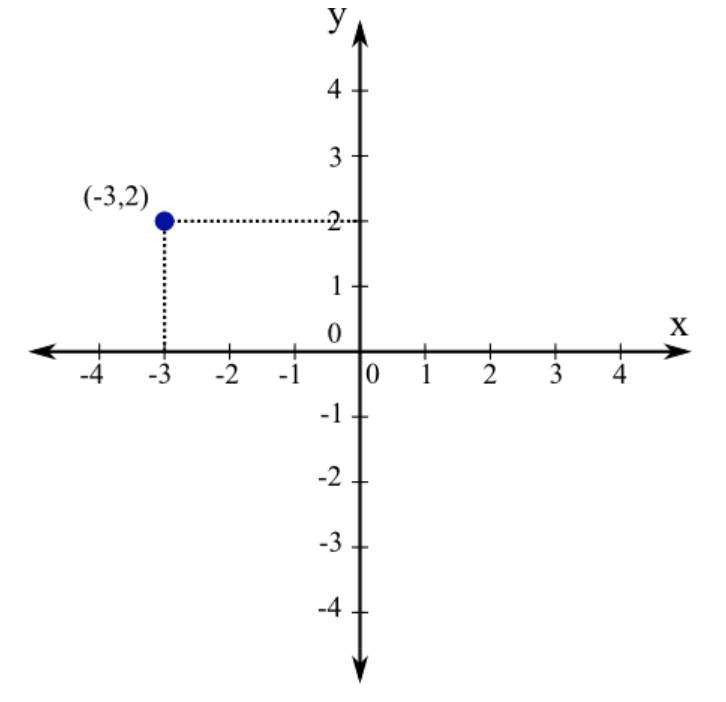
\includegraphics[scale=0.5]{Figures/appendixA_cartesian2D.png}
    \caption{Καρτεσιανές συντεταγμένες στο επίπεδο. The Cartesian coordinates (x,y) of the blue point specify its location relative to the origin, which is the intersection of the x- and y-axis.}
    \label{fig:apxA_cartesian2D}
\end{figure}


\subsection{Καρτεσιανές συντεταγμένες στον χώρο}
In three-dimensional space, the Cartesian coordinate system is based on three mutually perpendicular coordinate axes: the x-axis, the y-axis, and the z-axis, illustrated below. The three axes intersect at the point called the origin. You can imagine the origin being the point where the walls in the corner of a room meet the floor. The x-axis is the horizontal line along which the wall to your left and the floor intersect. The y-axis is the horizontal line along which the wall to your right and the floor intersect. The z-axis is the vertical line along which the walls intersect.

\begin{figure}[h]
    \centering
    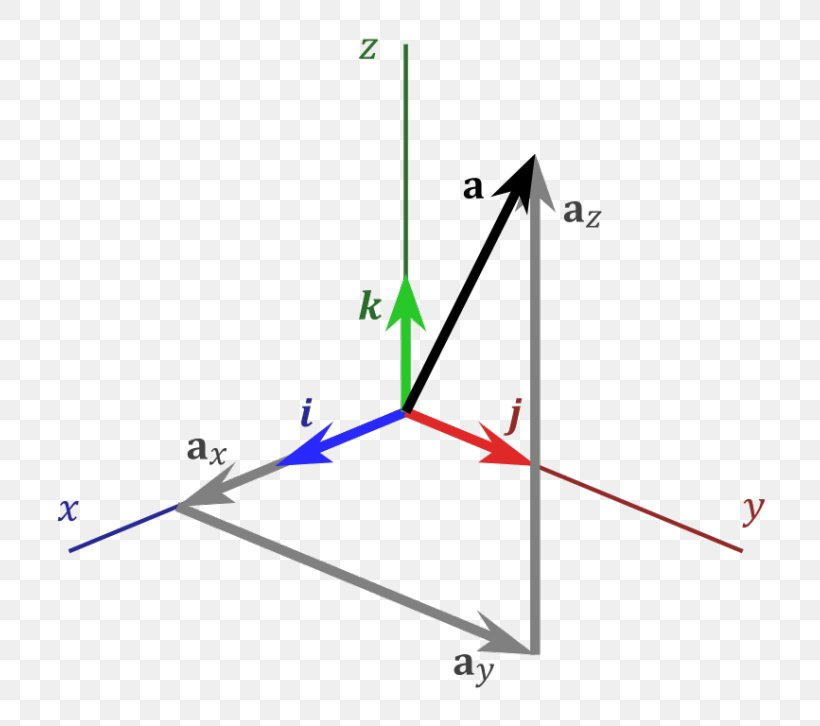
\includegraphics[scale=0.3]{Figures/appendixA_cartesian3D.jpg}
    \caption{Καρτεσιανές συντεταγμένες στον χώρο.}
    \label{fig:apxA_cartesian3D}
\end{figure}

With above definitions of the positive x, y, and z-axis, the resulting coordinate system is called right-handed; if you curl the fingers of your right hand from the positive x-axis to the positive y-axis, the thumb of your right hand points in the direction of the positive z-axis. Switching the locations of the positive x-axis and positive y-axis creates left-handed coordinate system. The right-handed and left-handed coordinate systems represent two equally valid mathematical universes. The problem is that switching universes will change the sign on some formulas. Since these pages are written in the right-handed universe, we suggest you live in our universe while studying from these pages.

In addition to the three coordinate axes, we often refer to three coordinate planes. The xy-plane is the horizontal plane spanned by the x and y-axes. It is identical to the two-dimensional coordinate plane and contains the floor in the room analogy. Similarly, the xz-plane is the vertical plane spanned by the x and z-axes and contains the left wall in the room analogy. Lastly, the yz-plane is the vertical plane spanned by the y and the z-axis and contains the right wall in the room analogy.
\\
{\color{red} \hrule}
Cartesian coordinates can be used not only to specify the location of points, but also to specify the coordinates of vectors. The Cartesian coordinates of two or three-dimensional vectors look just like those of points in the plane or three-dimensional space.

Από το σχήμα \ref{fig:apxA_cartesian3D} προκύπτει ότι το διάνυσμα θέσεως ,$\boldsymbol{a}$, θα δίνεται από τη σχέση: $$\boldsymbol{a} = a_x \boldsymbol{i} + a_y \boldsymbol{j} + a_z \boldsymbol{k}$$

But, there is no reason to stop at three-dimensions. We could define vectors in four, five, or higher dimensions by just specifying four, five, or more Cartesian coordinates. We can't visualize these higher dimensions like we did with the above applets, but we can easily write down the list of numbers for the coordinates.\\
{\color{red} \hrule}


\section{Πολικές συντεταγμένες}
In two dimensions, the Cartesian coordinates (x,y) specify the location of a point P in the plane. Another two-dimensional coordinate system is polar coordinates. Instead of using the signed distances along the two coordinate axes, polar coordinates specifies the location of a point P in the plane by its distance r from the origin and the angle $\theta$ made between the line segment from the origin to P and the positive x-axis. The polar coordinates $(r, \theta)$ of a point P are illustrated in the below figure (Σχήμα \ref{fig:apxA_polar_coordinates}).

\begin{figure}[h]
   \centering
\begin{subfigure}[h]{0.45\textwidth}
	\centering
   	 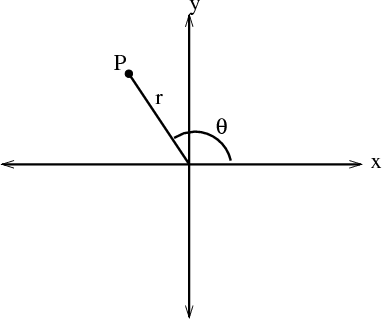
\includegraphics[width = \linewidth]{Figures/appendixA_polar_coordinates_whole.png} 
\end{subfigure}
\begin{subfigure}[h]{0.4\textwidth}
	\centering
	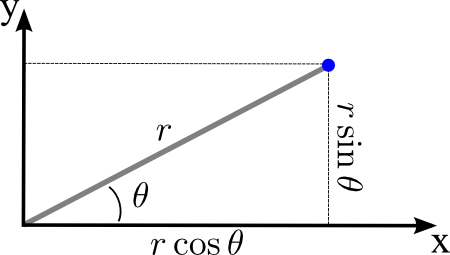
\includegraphics[width = \linewidth]{Figures/appendixA_polar_coordinates.png} 
    \end{subfigure}
    \caption{Πολικές συντεταγμένες στο επίπεδο.}
    \label{fig:apxA_polar_coordinates}
\end{figure}

As r ranges from 0 to infinity and $\theta$ ranges from 0 to $2\pi$, the point P specified by the polar coordinates $(r, \theta)$ covers every point in the plane. Adding $2\pi$ to $\theta$ brings us back to the same point, so if we allowed $\theta$ to range over an interval larger than $2\pi$, each point would have multiple polar coordinates. Hence, we typically restrict $\theta$ to be in the interval $0\leq \theta \leq 2\pi$. However, even with that restriction, there still is some non-uniqueness of polar coordinates: when $r=0$, the point P is at the origin independent of the value of $\theta$.

We can calculate the Cartesian coordinates of a point with polar coordinates $(r, \theta)$ by forming the right triangle illustrated in Figure \ref{fig:apxA_polar_coordinates}.  The hypotenuse is the line segment from the origin to the point, and its length is r. The projection of this line segment on the x-axis is the leg of the triangle adjacent to the angle $\theta$, so $x=r \cos \theta$. The y-component is determined by the other leg, so $y = r \sin \theta$. Our conversion formula is:
\begin{eqnarray}
    x &=& r \cos \theta \\
    y &=& r \sin \theta 
\end{eqnarray}

Για τους αντίστροφους μετασχηματισμούς προκύπτει από τις παραπάνω σχέσεις ότι:
\begin{eqnarray}
    x^2 + y^2 &=& r^2 (\cos^2 \theta + \sin^2 \theta) = r^2 \Rightarrow r = \sqrt{x^2 + y^2} \\ \nonumber \\
    \frac{y}{x} &=& \frac{r \sin \theta}{r \cos \theta} = \tan \theta \Rightarrow \theta = \arctan \left( \frac{y}{x} \right)
\end{eqnarray}

Παρατηρούμε ότι με βάση τη σχέση Α.4 για το σημείο $(x,y) = (0,0)$, η γωνία $\theta$ δεν ορίζεται. Σε αυτή την περίπτωση όμως παίρνουμε ότι $\theta = 0$.


\section{Κυλινδρικές συντεταγμένες}
Cylindrical coordinates are a simple extension of the two-dimensional polar coordinates to three dimensions. They simply combine the polar coordinates in the xy-plane with the usual z coordinate of Cartesian coordinates. To form the cylindrical coordinates of a point P, simply project it down to a point Q in the xy-plane (Σχήμα \ref{fig:apxA_cylindrical_coordinates}). Then, take the polar coordinates $(r, \theta)$ of the point Q, i.e., r is the distance from the origin to Q and $\theta$ is the angle between the positive x-axis and the line segment from the origin to Q. The third cylindrical coordinate is the same as the usual z-coordinate. It is the signed distance of the point P to the xy-plane (being negative is P is below the xy-plane). The below figure illustrates the cylindrical coordinates $(r, \theta, z)$ of the point P.

\begin{figure}[h]
    \centering
    \includegraphics[scale=0.5]{Figures/appendixA_cylindrical_coordinates.png}
    \caption{Κυλινδρικές συντεταγμένες στον χώρο.}
    \label{fig:apxA_cylindrical_coordinates}
\end{figure}

Οι μετασχηματισμοί δίνονται από τις σχέσεις:
\begin{eqnarray}
    x &=& r \cos \theta \\
    y &=& r \sin \theta \\
    z &=& z
\end{eqnarray}
ενώ για τους αντίστροφους μετασχηματισμούς, ισχύουν οι σχέσεις Α.3 και Α.4.

\section{Σφαιρικές συντεταγμένες}
Spherical coordinates can be a little challenging to understand at first. Spherical coordinates determine the position of a point in three-dimensional space based on the distance $\rho$ from the origin and two angles $\theta$ and $\phi$. If one is familiar with polar coordinates, then the angle $\theta$ isn't too difficult to understand as it is essentially the same as the angle $\theta$ from polar coordinates. But some people have trouble grasping what the angle $\phi$ is all about\footnote{Όλο το παράρτημα είναι μετάφραση της σελίδας \url{https://mathinsight.org/spherical_coordinates}, η οποία περιέχει και διάφορα applets για την καλύτερη κατανόηση των εννοιών.}. Στη συνέχεια θα εξάγουμε τις σχέσεις μεταξύ Καρτεσιανών και σφαιρικών συντενταγμένων.

Οι σφαιρικές συντεταγμένες ορίζονται βάσει του σχήματος \ref{fig:apxA_spherical_coordinates}, το οποίο δείχνει τις σφαιρικές συντεταγμένες στο σημείο P.

\begin{figure}[h]
    \centering
    \includegraphics[scale=0.5]{Figures/appendixA_spherical_coordinates_simple.png}
    \caption{Σφαιρικές συντεταγμένες στον χώρο.}
    \label{fig:apxA_spherical_coordinates}
\end{figure}

The coordinate $\rho$ is the distance from P to the origin. If the point Q is the projection of P to the xy-plane, then $\theta$ is the angle between the positive x-axis and the line segment from the origin to Q. Lastly, $\phi$ is the angle between the positive z-axis and the line segment from the origin to P.

We can calculate the relationship between the Cartesian coordinates $(x, y, z)$ of the point P and its spherical coordinates $(\rho, \theta, \phi)$ using trigonometry. Το ροζ τρίγωνο του Σχήματος \ref{fig:apxA_spherical_coordinates_derivation} is the right triangle whose vertices are the origin, the point P, and its projection onto the z-axis. As the length of the hypotenuse is $\rho$ and $\phi$ is the angle the hypotenuse makes with the z-axis leg of the right triangle, the z-coordinate of P (i.e., the height of the triangle) is $z = \rho \cos \phi$. The length of the other leg of the right triangle is the distance from P to the z-axis, which is $r = \rho \sin \phi$. The distance of the point Q from the origin is the same quantity.

\begin{figure}[h]
    \centering
    \includegraphics[scale=0.5]{Figures/appendixA_spherical_coordinates_analytical.png}
    \caption{Σχέση Καρτεσιανών και σφαιρικών συντενταγμένων.}
    \label{fig:apxA_spherical_coordinates_derivation}
\end{figure}

The cyan triangle, shown in both the original 3D coordinate system on the left and in the xy-plane on the right, is the right triangle whose vertices are the origin, the point Q, and its projection onto the x-axis. In the right plot, the distance from Q to the origin, which is the length of hypotenuse of the right triangle, is labeled just as r. As $\theta$ is the angle this hypotenuse makes with the x-axis, the x- and y-components of the point Q (which are the same as the x- and y-components of the point P) are given by $x = r \cos \theta$ and $y = r \sin \theta$. Since $r = \rho \sin \phi$, these components can be rewritten as $x = \rho \sin \phi \cos \theta$ and $y = \rho \sin \phi \sin \theta$. In summary, the formulas for Cartesian coordinates in terms of spherical coordinates are:

\begin{eqnarray}
    x &=& \rho \sin \phi \cos \theta \\
    y &=& \rho \sin \phi \sin \theta \\
    z &=& \rho \cos \phi
\end{eqnarray}
όπου $\rho \geq 0, 0 \leq \theta \leq 2\pi, 0 \leq \phi \leq \pi$.

Unfortunately, the convention for the notation of spherical coordinates is not standardized across disciplines. For example, in physics, the roles of $\theta$ and $\phi$ are typically reversed. In order to correctly understand someone's use of spherical coordinates, you must first determine what notational convention this are using. You cannot assume they follow the convention used here.

%     \chapter{Κινητική θεωρία και εξισώσεις κατάστασης}
\label{apx:kinetic_theory}

\section{Γενικές έννοιες}
\label{apx:sec:general}
Σε αυτό το Κεφάλαιο θα δώσουμε συνοπτικά κάποιες βασικές έννοιες Θερμοδυναμικής και Στατιστικής Φυσικής που θα χρησιμοποιηθούν τόσο για την κλασική όσο και για την κβαντική περιγραφή των αερίων.

\textbf{1ος θερμοδυναμικός νόμος}: Το πρώτο θερµοδυναµικό αξίωµα µπορεί να διατυπωθεί ως εξής: "\textit{Η θερµότητα
είναι µια µορφή ενέργειας, και η ενέργεια διατηρείται}". Αν σε ένα αέριο προσθέσουµε θερµότητα, $\dbar Q$, τότε στη γενικότερη περίπτωση, θα αυξηθεί ταυτόχρονα και η εσωτερική του ενέργεια κατά $dU$ και θα µεταβληθεί ο όγκος του κατά $dV$ καταναλώνοντας ενέργεια $\dbar W = P dV$. Με άλλα λόγια, το ποσό θερμότητας που απορροφά ή αποβάλλεται από ένα θερμοδυναμικό σύστημα είναι ίσο με το αλγεβρικό άθροισμα της μεταβολής της εσωτερικής ενέργειας και του έργου που δαπανά ή παράγει το σύστημα.
Το πρώτο θερµοδυναµικό αξίωµα µε βάση τα παραπάνω µπορεί να περιγραφεί από την εξίσωση\footnote{Προσέξτε ότι τα $\dbar Q$ και $\dbar W$ είναι μη-τέλεια διαφορικά (inexact differentials). Αυτό σημαίνει ότι οι ποσότητες $Q,W$ δεν είναι καταστατικές συναρτήσεις αλλά εξαρτώνται από την διαδρομή (path functions) και άρα και τα διαφορικά τους εξαρτώνται και αυτά από τη διαδρομή.}
\begin{equation}
    \dbar Q = dU + \dbar W = dU + P dV
\end{equation}

\textbf{2ος θερμοδυναμικός νόμος}: Για μία αντιστρεπτή μεταβολή, η αλλαγή στην εντροπία ισούται με την αλλαγή στο ποσό θερμότητας δια την θερμοκρασία
\begin{equation}
    dS = \frac{\dbar Q}{T}
\end{equation}


\textbf{Εσωτερική ενέργεια}: Ονομάζεται το άθροισμα της ενέργειας όλων των ατόμων, μορίων και ιόντων ενός συστήματος. Η εσωτερική ενέργεια περιλαμβάνει πάντα τους παρακάτω όρους:
\begin{itemize}
    \item Κινητική ενέργεια λόγω της άτακτης κίνησης των σωματιδίων (γνωστή και ως θερμική κίνηση) --- translational energy
    \item Ενέργεια λόγω της περιστροφικής κίνησης των μορίων --- rotational energy
    \item Ενέργεια δόνησης των ατόμων στο μόριο --- vibrational energy
    \item Δυναμική ενέργεια λόγω των ελκτικών ή απωστικών δυνάμεων ανάμεσα στα άτομα, μόρια ή ιόντα του συστήματος --- potential energy
\end{itemize}

\textbf{Ιδανικό αέριο}: Ένα υποθετικό αέριο που αποτελείται από μη-διαχωρίσιμα σημειακά σωματίδια τα οποία συγκρούονται ελαστικά και για τα οποία οι διασωματιδιακές δυνάμεις μπορούν να αγνοηθούν. Ένα ιδανικό αέριο υπακούει στο \textbf{νόμο των ιδανικών αερίων}
\begin{equation}
    PV = NkT \Rightarrow P = \frac{\rho}{\mu m_H} kT
\end{equation}

Για το ιδανικό αέριο, θεωρούμε ότι τα σωματίδια που το αποτελούν δεν έχουν εσωτερική δομή, άρα εσωτερικοί μηχανισμοί όπως η δόνηση και η περιστροφή δεν συνεισφέρουν στην εσωτερική ενέργεια. Επίσης, η ενέργεια του σωματιδίου δεν εξαρτάται από τη θέση του, άρα δεν υπάρχει και συνεισφορά από "συντεταγμένες". Αυτό μας αφήνει μόνο με την κινητική ενέργεια. Δηλαδή, για ένα ιδανικό αέριο, η εσωτερική του ενέργεια ισούται με την κινητική ενέργεια και χαρακτηρίζεται πλήρως από αυτήν.
\begin{equation}
    \langle U \rangle = \langle E_{\text{kin}} \rangle = \frac{3}{2} NkT
\end{equation}
όπου $N$ ο αριθμός των σωματιδίων.

Στις τρεις διαστάσεις, υπάρχουν 3 ανεξάρτητες διευθύνσεις για την ορμή: $p_x, p_y, p_z$. Σύμφωνα με το θεώρημα της ισοκατανομής (equipartition theorem) η μέση ενέργεια ανά σωματίδιο
\begin{equation}
    \frac{\langle U \rangle}{N} = \frac{3}{2}kT
\end{equation}
μοιράζεται ισόποσα σε κάθε βαθμό ελευθερίας, ώστε σε κάθε διεύθυνση να αντιστοιχεί $\frac{1}{2}kT$

\textbf{Αδιαβατικές διεργασίες}: Συχνά ερχόμαστε αντιμέτωποι με διεργασίες οι οποίες συμβαίνουν σε τόσο σύντομο χρονικό διάστημα (π.χ. σε δυναμικό χρόνο) ώστε δεν υπάρχει ανταλλαγή θερμότητας με το περιβάλλον ($\dbar Q = dS = 0$). Αυτές οι διεργασίες ονομάζοναι "αδιαβατικές" και υπακούουν σε μία σχέση της μορφής
\begin{equation}
    P \propto \rho^{\gamma} 
\end{equation}
όπου το $\gamma$ ονομάζεται "αδιαβατικός δείκτης" (adiabatic index) 
\begin{equation}
    \gamma = \frac{q+5}{q+3}
\end{equation}
όπου $q$ ο αριθμός των εσωτερικών βαθμών ελευθερίας (για ιδανικό αέριο που τα σωματίδια είναι σημειακά έχουμε $q = 0 \rightarrow \gamma = 5/3)$.

\textbf{Θερμοδυναμική ισορροπία}: Ένα σύστημα λέγεται ότι βρίσκεται σε κατάσταση θερμοδυναμικής ισορροπίας όταν βρίσκεται σε
\begin{itemize}
    \item \textbf{μηχανική ισορροπία}: το διανυσματικό άθροισμα όλων των εξωτερικών και εσωτερικών δυνάμεων είναι μηδέν.
    \item \textbf{θερμική ισορροπία}: ένα σύστημα είναι σε θερμική ισορροπία με τον εαυτό του όταν δεν υπάρχουν θερμοβαθμίδες. Δύο συστήματα βρίσκονται σε θερμική ισορροπία μεταξύ τους όταν δεν υπάρχει μεταφορά θερμότητας. Για ένα αέριο συγκεκριμένης θερμοκρασίας που βρίσκεται σε θερμική ισορροπία, ισχύει η κατανομή Maxwell-Boltzmann για την κατανομή των ταχυτήτων των σωματιδίων που το αποτελούν.
    \item \textbf{χημική ισορροπία}: σε μια χημική αντίδραση, η κατάσταση χημικής ισορροπίας είναι αυτή κατά την οποία τόσο τα αντιδρώντα όσο και τα προϊόντα βρίσκονται σε συγκεντρώσεις που δεν υπάρχει η τάση για αλλαγή με τον χρόνο. Συνήθως αυτή η κατάσταση επέρχεται όταν ο ρυθμός παραγωγής των προϊόντων ισούται με τον ρυθμό της αντίστροφης διαδικασίας κατά την οποία τα προϊόντα σχηματίζουν ξανά τα αντιδρώντα από τα οποία προήλθαν.
    \item \textbf{στατιστική ισορροπία}: ένα σύστημα βρίσκεται σε κατάσταση στατιστικής ισορροπίας όταν ο πληθυσμός των ατόμων και των ιόντων που το αποτελούν δεν αλλάζει με τον χρόνο. Σε ένα τέτοιο σύστημα, ο πληθυσμός των καταστάσεων δίνεται από τον νόμο του Boltzmann.
\end{itemize}
Σε μία κατάσταση θερμοδυναμικής ισορροπίας, δεν υπάρχει ροή ενέργειας ή ύλης, δεν υπάρχουν αλλαγές φάσης ή δυναμικά που θα οδηγήσουν σε αλλαγές μέσα στο σύστημα. Ένα τέτοιο σύστημα δεν υπόκειται σε καμία αλλαγή όταν βρίσκεται απομονωμένο από το περιβάλλον του. Αν το σύστημα είναι απομονωμένο τόσο για την ύλη όσο και για την ακτινοβολία, και βρίσκεται σε κατάσταση μηχανικής ισορροπίας, τότε σταδιακά θα επέλθει σε κατάσταση θερμοδυναμικής ισορροπίας. Τέλος, για ένα σύστημα που βρίσκεται σε κατάσταση θερμοδυναμικής ισορροπίας, η θερμοκρασία ακτινοβολίας $T_R$, η θερμοκρασία λόγω της κινητικής ενέργειας των σωματιδίων $T$, καθώς και η θερμοκρασία διέγερσης $T_{\text{ex}}$ είναι ίσες μεταξύ τους.

\textbf{Τοπική θερμοδυναμική ισορροπία}: Πραγματική θερμοδυναμική ισορροπία είναι δύσκολο να επιτευχθεί (σχεδόν σε όλες τις περιπτώσεις ενέργεια διαφεύγει από το σύστημα με τη μορφή ακτινοβολίας, δηλαδή το σύστημα ψύχεται), και συχνά υπάρχουν θερμοβαθμίδες. Παρόλα αυτά, σε πολλά συστήματα (π.χ. αστέρες, μεσοασαστρικό μέσο) μπορούμε να εφαρμόσουμε τοπική θερμοδυναμική ισορροπία, που σημαίνει ότι το σύστημα βρίσκεται σε θερμοδυναμική ισορροπία αλλά μόνο σε μια πολύ μικρή περιοχή ενδιαφέροντος. Σε ένα σύστημα που βρίσκεται σε κατάσταση τοπικής θερμοδυναμικής ισορροπίας, υπάρχουν βαθμίδες θερμοκρασίας, πυκνότητας, πίεσης κτλ, αλλά θα είναι αρκετά μικρές στο διάστημα που ορίζεται από τη μέση ελεύθερη διαδρομή ενός σωματιδίου του αερίου.
Το γεγονός ότι τα φωτόνια στο εσωτερικό του Ήλιου κάνουν πολλές χιλιάδες χρόνια να φτάσουν στην επιφάνεια και άρα είναι τοπικώς "παγιδευμένα" είναι αποτέλεσμα της κατάστασης τοπικής θερμοδυναμικής ισορροπίας που επικρατεί στο εσωτερικό του Ήλιου.

\subsection{Καταστατικές εξισώσεις αερίων}
Ως καταστατική εξίσωση εννοούμε μία θερμοδυναμική εξίσωση που περιγράφει την κατάσταση της ύλης υπό συγκεκριμένες φυσικές συνθήκες. Συνήθως είναι της μορφής $P = P(\rho, T)$. Πολλές φορές είναι χρήσιμο να γράψουμε την καταστατική εξίσωση σε διαφορική μορφή. Η διαφορική μορφή μπορεί να βρεθεί αν ξεκινήσουμε γράφοντας την καταστατική εξίσωση γενικά ως έναν εκθετικό νόμο (power law)
\begin{equation}
    P = \rho^{\chi_\rho} T^{\chi_T}
\end{equation}
και άρα το ολικό διαφορικό είναι
\begin{align}
    \nonumber dP &= \left( \frac{\partial P}{\partial \rho} \right)_T d\rho + \left( \frac{\partial P}{\partial T} \right)_\rho dT \Rightarrow \\\nonumber\\
    \nonumber &\Rightarrow dP = \chi_\rho T^{\chi_T} \rho^{\chi_\rho - 1} d\rho +  \chi_T \rho^{\chi_\rho} T^{\chi_T - 1} dT \Rightarrow \\\nonumber\\
    \nonumber &\Rightarrow dP = \underbrace{\rho^{\chi_\rho} T^{\chi_T}}_{P} \left(\chi_\rho \rho^{-1} d\rho + \chi_T T^{-1} dT \right) \Rightarrow \\\nonumber\\
    &\Rightarrow \boxed{\frac{dP}{P} = \chi_\rho \frac{d\rho}{\rho} + \chi_T \frac{dT}{T}}
\end{align}

Αντιπαραβάλοντας τις σχέσεις
\begin{align*}
    \label{apx:eq:differential_form_of_eos}
    dP &= \left( \frac{\partial P}{\partial \rho} \right)_T d\rho + \left( \frac{\partial P}{\partial T} \right)_\rho dT \\\\
    \frac{dP}{P} &= \chi_\rho \frac{d\rho}{\rho} + \chi_T \frac{dT}{T}
\end{align*}
βρίσκουμε ότι τα εκθετικά $\chi_\rho, \chi_T$ δίνονται από τις σχέσεις
\begin{align*}
    \chi_\rho &= \frac{\rho}{P} \left( \frac{\partial P}{\partial \rho} \right)_T \\\\
    \chi_T &= \frac{T}{P} \left( \frac{\partial P}{\partial T} \right)_\rho
\end{align*}

Μπορεί κανείς όμως να βρει μία ακόμα πιο κομψή έκφραση των παραπάνω εκθετών ως εξής:
\begin{align*}
     P &= \rho^{\chi_\rho} T^{\chi_T} \Rightarrow \log \,P = \log \,\left( \rho^{\chi_\rho} T^{\chi_T} \right) = \log \,\rho^{\chi_\rho} + \log \,T^{\chi_T} \Rightarrow \\\\
     &\Rightarrow \log \,P = \chi_\rho \log \,\rho + \chi_T \log \,T
\end{align*}
Το ολικό διαφορικό άρα είναι
\begin{equation*}
    d\log \,P = \left( \frac{\partial \log \,P}{\partial \log \,\rho} \right)_T d \log \,\rho + \left( \frac{\partial \log \,P}{\partial \log \,T} \right)_\rho d \log \,T
\end{equation*}
ώστε
\begin{equation*}
    d \log \,P = \chi_\rho d\log \,\rho + \chi_T d \log \,T
\end{equation*}
και με αντιπαραβολή των δύο τελευταίων σχέσεων προκύπτει τελικά ότι
\begin{align}
    \chi_\rho &= \frac{\rho}{P} \left( \frac{\partial P}{\partial \rho} \right)_T = \left( \frac{\partial \log \,P}{\partial \log \,\rho} \right)_T \label{apx:eq:chi_rho}\\\nonumber\\
    \chi_T &= \frac{T}{P} \left( \frac{\partial P}{\partial T} \right)_\rho = \left( \frac{\partial \log \,P}{\partial \log \,T} \right)_\rho \label{apx:eq:chi_T}
\end{align}

Στην πιο γενική περίπτωση, τα $\chi_\rho, \chi_T$ εξαρτώνται και τα ίδια από τα $\rho, T$ αλλά αν είναι (προσεγγιστικά) σταθερά, η καταστατική εξίσωση γράφεται
\begin{equation}
    \label{apx:eq:eos_chi_rho_chi_T}
    P = P_0 \,\rho^{\chi_\rho} \,T^{\chi_T}
\end{equation}

Στην συνέχεια θα εξάγουμε την καταστατική εξίσωση για ένα τέλειο αέριο από τις αρχές της στατιστικής μηχανικής. Έστω $n(p)$ η κατανομή των ορμών των σωματιδίων του αερίου, δηλαδή με άλλα λόγια, το $n(p)dp$ αναπαριστά τον αριθμό των σωματιδίων ανά μονάδα όγκου που έχουν ορμή $p \in [p, p+dp]$. Αν η $n(p)$ είναι γνωστή, τότε η αριθμητική πυκνότητα, η πυκνότητα (εσωτερικής) ενέργειας, και η πίεση θα δίνονται από τα ακόλουθα ολοκληρώματα:
\begin{align}
    n &= \int_{0}^{\infty} n(p) dp \label{apx:eq:number_density_integral} \\\nonumber\\
    u &= \int_{0}^{\infty} E_{\text{kin}} n(p) dp = n \langle E_{\text{kin}} \rangle \label{apx:eq:energy_density_integral} \\\nonumber\\
    P &= \frac{1}{3}\int_{0}^{\infty} p \,v_p \,n(p) dp = \frac{1}{3} n \langle p \,v_p \rangle \label{apx:eq:pressure_integral} 
\end{align}
όπου $E_{\text{kin}}$ η κινητική ενέργεια σωματιδίου με ορμή $p$ και ταχύτητα $v_p$. Η σχέση \eqref{apx:eq:number_density_integral} είναι τετριμμένη ενώ η σχέση \eqref{apx:eq:energy_density_integral} προκύπτει από τον ορισμό του ιδανικού αερίου. Όμως η σχέση \eqref{apx:eq:pressure_integral} χρειάζεται εξήγηση.

\begin{figure}[h]
    \centering
    \includegraphics[scale = 0.6]{Figures/elastic_collision_in_a_box.png}
    \caption{Σωματίδιο αερίου μέσα σε ένα κυβικό κουτί όγκου $1 \,\text{cm}^3$. Κάθε σύγκρουση με τα τοιχώματα του κουτιού οδηγεί σε μεταφορά ορμής. Η πίεση μέσα στο κουτί είναι το αποτέλεσμα της συνολικής μεταφοράς ορμής από όλα τα σωματίδια μέσα στο κουτί.}
    \label{apx:fig:elastic_collisions}
\end{figure}

Ας υποθέσουμε ένα αέριο που αποτελείται από $N$ σωματίδια και το οποίο περιέχεται σε κυβικό κουτί με μήκος πλευρών $L = 1 \,\text{cm}$. Κάθε σωματίδιο ανακλάται από τα τοιχώματα του κουτιού και η πίεση στην συγκεκριμένη επιφάνεια είναι το αποτέλεσμα της μεταφοράς της ορμής από όλα τα σωματίδια που συγκρούονται με αυτή. Έστω ένα σωματίδιο με ορμή $p$ και αντίστοιχη ταχύτητα $v_p$ το οποίο πλησιάζει την μία πλευρά του κουτιού υπο γωνία $\theta$, όπως φαίνεται στο σχήμα \ref{apx:fig:elastic_collisions}. Ο χρόνος μεταξύ δύο συγκρούσεων στην ίδια επιφάνεια του κουτιού είναι
\begin{equation*}
    \Delta t = \frac{2L}{v_p \cos \,\theta} = \frac{2}{v_p \cos \,\theta}
\end{equation*}
Επειδή οι συγκρούσεις είναι ελαστικές ($p_f = - p_i$) η μεταφορά ορμής είναι διπλάσια από τη συνιστώσα της ορμής που είναι κάθετη στην επιφάνεια
\begin{equation*}
    \Delta p = p_f - p_i = 2p \cos \,\theta
\end{equation*}
'Αρα, ο ρυθμός με τον οποίο μεταφέρεται ορμή ανά σωματίδιο είναι
\begin{equation*}
    \frac{\Delta p}{\Delta t} = p \,v_p \,\cos^2 \,\theta
\end{equation*}
Ο αριθμός των σωματιδίων με $p \in [p,p+dp]$ και $\theta \in [\theta, \theta+d\theta]$ συμβολίζεται με $n(p, \theta) dp \,d\theta$. Η συνεισφορά αυτών των σωματιδίων στην πίεση τότε είναι
\begin{equation*}
    dP =  p \,v_p \,\cos^2 \,\theta \,n(p, \theta) dp \,d\theta
\end{equation*}
Επειδή οι ορμές είναι κατανεμημένες ισοτροπικά σε όλες τις διευθύνσεις μέσα σε μια στερεά γωνία $2\pi$, και η στερεά γωνία $d\omega$ που αντιστοιχεί σε αυτά τα σωματίδια με $\theta \in [\theta, \theta+d\theta]$ ισούται με $2\pi \sin \,\theta \,d\theta$ έχουμε ότι $n(p, \theta) = n(p) \sin \,\theta \,d\theta$ και άρα
\begin{equation*}
    dP = p v_p \cos^2 \,\theta \,n(p) \sin \,\theta \,d\theta \,dp
\end{equation*}
Η συνολική πίεση βρίσκεται με ολοκλήρωση σε όλες τις γωνίες ($0 \leq \theta \leq \pi/2$) και ορμές ώστε
\begin{align*}
    P &= \int_{0}^{\frac{\pi}{2}} \int_{0}^{\infty} p v_p \cos^2 \,\theta \,n(p) \sin \,\theta \,d\theta \,dp = \\\\
    &=\int_{0}^{\frac{\pi}{2}} \cos^2 \,\theta \,\sin \,\theta \,d\theta \int_{0}^{\infty} p v_p n(p) dp = \\\\
    &= \int_{0}^{1} \cos^2 \,\theta \, d(\cos \,\theta) \int_{0}^{\infty} p v_p n(p) dp \Rightarrow \\\\
    &\Rightarrow P = \frac{1}{3} \int_{0}^{\infty} p v_p n(p) dp = \frac{1}{3} n \langle p v_p \rangle
\end{align*}

Έχοντας ξεκαθαρίσει τα παραπάνω, θέλουμε τώρα να βρούμε μία σχέση μεταξύ της πίεσης και της εσωτερικής ενέργειας. Σύμφωνα με την ειδική σχετικότητα, η ορμή και η ταχύτητα των σωματιδίων σχετίζονται με την ενέργειά τους σύμφωνα με τις σχέσεις:
\begin{equation}
    \epsilon^2 = p^2 c^2 + m^2 c^4
\end{equation}
\begin{align}
    \nonumber \frac{\partial}{\partial p} (\epsilon^2) &= \frac{\partial}{\partial p} (p^2 c^2 + m^2 c^4) \Rightarrow 2\epsilon \frac{\partial \epsilon}{\partial p} = 2p c^2 \Rightarrow \\\nonumber\\
    &\Rightarrow \frac{\partial \epsilon}{\partial p} \equiv v_p = \frac{pc^2}{\epsilon}
\end{align}
Χρησιμοποιώντας αυτές τις σχέσεις μπορούμε να βρούμε σχέσεις μεταξύ της πίεσης και της εσωτερικής ενέργειας ενός ιδανικού αερίου στο μη-σχετικιστικό (NR) όριο και στο εξαιρετικά σχετικιστικό (ER) όριο:

\begin{itemize}
    \item \textbf{NR όριο}: σε αυτή την περίπτωση οι ορμές είναι $p \ll mc$
    
    $$\epsilon^2 = p^2 c^2 + m^2 c^4 \Rightarrow \epsilon^2 = c^2 \left(p^2 + m^2c^2 \right)$$
    Επειδή ισχύει ότι $p \ll mc$, άρα $\epsilon \simeq mc^2$ και συνεπώς
    $$v_p = \frac{pc^2}{\epsilon} = \frac{p}{m}$$
    Η κινητική ενέργεια είναι όπως περιμένουμε $E_{\text{kin}} = \frac{p^2}{2m}$ οπότε $\langle p v_p \rangle = \langle \frac{p^2}{m} \rangle = 2 \langle E_{\text{kin}} \rangle $.
    
    Τελικά, από τις σχέσεις \eqref{apx:eq:energy_density_integral}, \eqref{apx:eq:pressure_integral}, προκύπτει
    \begin{equation}
        \label{apx:eq:pressure_internal_energy_relation_for_nr_case}
        \boxed{P = \frac{2}{3}u}
    \end{equation}
    
    \item \textbf{ER όριο}: σε αυτή την περίπτωση έχουμε $p \gg mc$
    
    Αυτό σημαίνει ότι $\epsilon = pc$ και άρα $v_p = c \longrightarrow \langle p v_p \rangle = \langle pc \rangle = \langle \epsilon \rangle$.
    
    Τελικά, από τις σχέσεις \eqref{apx:eq:energy_density_integral}, \eqref{apx:eq:pressure_integral}, προκύπτει
    \begin{equation}
        \label{apx:eq:pressure_internal_energy_relation_for_er_case}
        \boxed{P = \frac{1}{3}u}
    \end{equation}
\end{itemize}

Γενικά μπορούμε να γράψουμε ότι 
\begin{equation}
    P = \zeta n \langle E \rangle
\end{equation}
όπου $\zeta = 2/3$ ή $\zeta = 1/3$ για το μη-σχετικιστικό και το σχετικιστικό όριο αντίστοιχα. Αυτό έρχεται σε συμφωνία με την διαίσθησή μας καθώς θα περιμέναμε η πίεση που προέρχεται από την σύγκρουση (λόγω ταχυτήτων) σωματιδίων να είναι ανάλογη της πυκνότητας των σωματιδίων και της κινητικής τους ενέργειας
\begin{equation*}
    P \sim n mv^2 \sim n E_{\text{kin}}
\end{equation*}


\subsubsection{Το κλασικό ιδανικό αέριο}
Σε ένα ιδανικό αέριο η κατανομή των ορμών δίνεται από την κατανομή Maxwell-Boltzmann
\begin{equation}
    n(p) dp = \frac{n}{(2\pi m kT)^{3/2}} \exp\left(- \frac{p^2}{2mkT}\right) 4\pi p^2 dp
\end{equation}
με την οποία θα ασχοληθούμε εκτενώς παρακάτω. Θα αποδείξουμε τότε ότι $\langle E_{\text{kin}} \rangle = \frac{3}{2} kT $ και άρα σύμφωνα με τη σχέση \eqref{apx:eq:pressure_internal_energy_relation_for_nr_case} ισχύει ότι\textbf{ η καταστατική εξίσωση ενός ιδανικού αερίου είναι}
\begin{equation}
    \boxed{P_{\text{gas}} = \frac{2}{3}u = \frac{2}{3} n \langle E_{\text{kin}} \rangle = nkT = \frac{\rho}{\mu m_H}kT}
\end{equation}
που είναι ο γνωστός νόμος των ιδανικών αερίων. Αυτό το αποτέλεσμα προήλθε θεωρώντας μη-σχετικιστικά κλασικά σωματίδια αλλά μπορεί να δειχτεί ότι η ίδια σχέση ισχύει και για σχετικιστικά κλασικά σωματίδια.

Παρατηρούμε ότι ο νόμος των ιδανικών αερίων προκύπτει από τη σχέση \eqref{apx:eq:eos_chi_rho_chi_T} για $\chi_\rho = \chi_T = 1$


\subsubsection{Το αέριο φωτονίων}
Στο Κεφάλαιο \ref{ch:Chapter4}, αποδείξαμε ότι η πυκνότητα ενέργειας της ακτινοβολίας είναι
\begin{equation}
    u = \alpha T^4
\end{equation}
Επειδή το αέριο φωτονίων είναι εξ' ορισμού σχετικιστικό, χρησιμοποιούμε τη σχέση \eqref{apx:eq:pressure_internal_energy_relation_for_er_case} για να βρούμε την \textbf{καταστατική εξίσωση ενός αερίου φωτονίων}
\begin{equation}
    \boxed{P_{\text{rad}} = \frac{1}{3}u = \frac{1}{3} \alpha T^4}
\end{equation}

Παρατηρούμε ότι η καταστατική εξίωση ενός αερίου φωτονίων προκύπτει από τη σχέση \eqref{apx:eq:eos_chi_rho_chi_T} για $\chi_\rho = 0$ και $\chi_T = 4$.



\subsubsection{Το κβαντικό αέριο}
(εκφυλισμενο μη-σχετικιστικο αεριο φερμιονιων, εκφυλισμενο σχετικιστικο αεριο φερμιονιων)





\section{Νόμος του Boltzmann}
Εαν έχουμε έναν μεγάλο αριθμό ατόμων σε ένα ζεστό, πυκνό αέριο, τα άτομα αυτά συνεχώς θα συγκρούονται μεταξύ τους με αποτέλεσμα να διεγείρονται σε διάφορα πιθανά ενεργειακά επίπεδα. Η διέγερση λόγω συγκρούσεων θα ακολουθηθεί από την αποδιέγερση των ατόμων με εκπομπή ακτινοβολίας (σε χρονική κλίμακα της τάξης των νανοδευτερολέπτων). Αν η θερμοκρασία και η πίεση παραμείνουν σταθερά, θα υπάρχει κάποιου είδους δυναμικής ισορροπίας μεταξύ των διεγέρσεων από τις συγκρούσεις και τις αποδιεγέρσεις, οδηγώντας σε μια συγκεκριμένη κατανομή των ατόμων στα διάφορα ενεργειακά επίπεδα. Όσο χαμηλότερη είναι η θερμοκρασία, τόσο πιο γρήγορα θα μειώνεται ο πληθυσμός των ατόμων που καταλαμβάνουν υψηλές ενεργειακές στάθμες. Μόνο στις πολύ υψηλές θερμοκρασίες θα μπορούν οι υψηλές ενεργειακές στάθμες να καταλαμβάνονται από έναν σημαντικό αριθμό ατόμων. Η εξίσωση Boltzmann περιγράφει ποιά θα είναι η κατανομή των ατόμων ανάμεσα σε διάφορα ενεργειακά επίπεδα, ως συνάρτηση της ενέργειας και της θερμοκρασίας\footnote{Οι πληροφορίες αντλήθηκαν από \url{https://phys.libretexts.org/Bookshelves/Astronomy__Cosmology/Book\%3A_Stellar_Atmospheres_(Tatum)}}. 

Ας φανταστούμε ένα κουτί (σταθερός όγκος) το οποίο περιέχει N άτομα, το καθένα από τα οποία έχει m δυνατά ενεργειακά επίπεδα. Ας υποθέσουμε ότι υπάρχουν $ N_j$ άτομα στο ενεργειακό επίπεδο $ E_j$. Ο συνολικός αριμός N των ατόμων δίνεται από τη σχέση
\begin{equation}
    \label{eq:apx:total_number_of_atoms}
     N = \sum_{i=1}^{m} N_i
\end{equation}
όπου ο ακέραιος θετικός δείκτης i τρέχει από το 1 μέχρι το m, συμπεριλαμβάνοντας την τιμή j.

Η συνολική εσωτερική ενέργεια του συστήματος U θα δίνεται από τη σχέση
\begin{equation}
    \label{eq:apx:internal_energy}
     U = \sum_{i=1}^{m} N_i E_i
\end{equation}

Τώρα, πρέπει να βρούμε πόσοι τρόποι υπάρχουν να κατανείμουμε N άτομα έτσι ώστε να υπάρχουν $ N_1$ στο πρώτο ενεργειακό επίπεδο, $ N_2$ στο δεύτερο κ.ο.κ. Θα συμβολίσουμε αυτόν τον αριθμό με $ \Omega$. Στην στατιστική φυσική το μέγεθος αυτό ονομάζεται στατιστικό βάρος και είναι ο αριθμός των (τρόπων) μικροκαταστάσεων που αντιστοιχούν στην ίδια (ενεργεια) μακροκατάσταση.
\begin{equation}
    \label{eq:apx:statistical_weight}
     \Omega = \frac{N!}{N_1! N_2! N_3! \dots N_j! \dots N_m!} = \frac{N!}{\prod_{i=1}^{m}N_i!}
\end{equation}
Η σχέση αυτή δεν είναι προφανής, γι' αυτό θα επιχειρησούμε να τη δικαιολογήσουμε εν μέρει. Ο αριθμός των τρόπων που μπορούμε να διαλέξουμε $ N_1$ άτομα από ένα σύνολο N ατόμων ώστε να καταλάβουν το πρώτο ενεργειακό επίπεδο, θα δίνεται από τον διωνυμικό συντελεστή $ \Omega_1 = {N \choose N_1}$. Για κάθε έναν από αυτούς τους τρόπους, πρέπει να ξέρουμε με πόσους τρόπους μπορούν να διαμοιραστούν $ N_2$ άτομα από τα εναπομείναντα $ N - N_1$ τα οποία θα καταλαμβάνουν την δεύτερη ενεργειακή στοιβάδα, οι οποίοι είναι $ \Omega_2 = {N - N_1 \choose N_2}$. Άρα, ο αριθμός των τρόπων με τους οποίους μπορούμε να κατανείμουμε τα άτομα στις δύο πρώτες ενεργειακές στοιβάδες, είναι το γινόμενο 
\begin{align*}
     \Omega &= { N \choose N_1} { N - N_1 \choose N_2} =  \frac{N!}{N_1! (N-N_1)!} \frac{(N-N_1)!}{N_2! (N-N_1 -N_2)!} \\\\
    &=  \frac{N!}{N_1!} \frac{1}{N_2!(N_2! - N_2!)} = \frac{N!}{N_1!N_2!}
\end{align*}
Συνεχίζοντας αυτή τη λογική, καταλήγουμε στον πολυωνυμικό συντελεστή
$$ \Omega = \prod_{i=1}^{m} \Omega_i =  { N \choose N_1} { N - N_1 \choose N_2} \dots = \frac{N!}{N_1!N_2! \dots N_m!}$$
Ίσως ο παραπάνω συλλογισμός γίνεται πιο αντιληπτός αν έχουμε στο μυαλό μας πως ο διωνυμικός συντελεστής μας δίνει τον αριθμό των υπαρκτών τρόπων να χωρίσουμε τις ποσότητες $ N_1$ και $ N - N_1$ από ένα σύνολο $ N$, σε δύο διακριτές καταστάσεις (two distinct bins). Ο πολυωνυμικός συντελεστής αντίστοιχα μας δίνει τον αριθμό των υπαρκτών τρόπων να χωρίσουμε τις ποσότητες $ N_1, N_2, \dots , N_m$ από ένα σύνολο $ N$, σε $ N$ διακριτές καταστάσεις ($ N$ distinct bins).

Τώρα πρέπει να βρούμε τους πιο πιθανούς διαμερισμούς, δηλαδή τους πιο πιθανούς αριθμούς $ N_1, N_2, \dots , N_m$. Ο πιο πιθανός καταμερισμός θα είναι αυτός που μεγιστοποιεί το $ \Omega$ ως προς το κάθε $ N_j$, και που υπόκειται στους περιορισμούς των σχέσεων \eqref{eq:apx:total_number_of_atoms} και \eqref{eq:apx:internal_energy}. Η εύρεση ακροτάτων μιας συνάρτησης υπό περιορισμούς, μας οδηγεί στην χρήση των πολλαπλασιαστών Lagrange. Επειδή όμως ο χειρισμός του παραγοντικού ($ N!$) είναι δύσκολος στην ανάλυση, θα βρούμε το μέγιστο του λογαρίθμου $ \ln{\Omega}$, χωρίς καμία ποιοτική διαφορά στο αποτέλεσμα. Παίρνοντας τον λογάριθμο της σχέσης \eqref{eq:apx:statistical_weight}, προκύπτει ότι
\begin{equation}
    \label{eq:apx:log_statistical_weight}
     \ln{\Omega} = \ln{N!} - \ln{N_1!} - \ln{N_2!} - \dots
\end{equation}

Χρησιμοποιώντας τον τύπο του Stirling:
\begin{equation}
    \label{eq:apx:stirling_formula}
     \ln{X!} = X \ln{X} - X
\end{equation}
στη σχέση \eqref{eq:apx:log_statistical_weight}, προκύπτει ότι
\begin{align}
    \label{eq:apx:non_factorial_terms_multiplicity}
   \nonumber  \ln{\Omega} &=  N \ln{N} - \cancel{ N} - (N_1 \ln{N_1} - \cancel{ N_1}) - (N_2 \ln{N_2} - \cancel{ N_2}) - \dots \\\nonumber \\
   \nonumber &=  N \ln{ N} -  N_1 \ln{ N_1} -  N_2 \ln{  N_2} - \dots \\ \nonumber \\
   &=  N \ln{N} - \sum_{i=1}^{m} N_i \ln{N_i}
\end{align}

Τώρα μπορούμε να προχωρήσουμε με την εύρεση του μεγίστου της συνάρτησης \eqref{eq:apx:non_factorial_terms_multiplicity}, ως προς μία από τις μεταβλητές, για παράδειγμα την $ N_j$, με τρόπο τέτοιο ώστε να είναι συνεπής με τους περιορισμούς των σχέσεων \eqref{eq:apx:total_number_of_atoms} και \eqref{eq:apx:internal_energy}. Χρησιμοποιώντας την μέθοδο των πολλαπλασιαστών Lagrange, έχουμε ότι για τον πιθανό αριθμό κατάληψης (most probable occupation number) του j ενεργειακού επιπέδου, ισχύει η σχέση:

\begin{equation}
    \label{eq:apx:occupation_number_condition}
     \frac{\partial \ln{\omega}}{\partial N_j} = \lambda \frac{\partial N}{\partial N_j} + \mu \frac{\partial U}{\partial N_j}
\end{equation}
Αναπτύσοντας τους όρους έχουμε:
\begin{align*}
    \frac{\partial \ln{\Omega}}{\partial N_j} &= \frac{\partial}{\partial N_j} \left( -N_j \ln{N_j}\right) = -\cancelto{1}{\frac{\partial N_j}{\partial N_j}} \ln{N_j} - \cancelto{1}{N_j \frac{\partial \ln{N_j}}{\partial N_j}} = - \ln{N_j} - 1 \\\\
    \lambda \frac{\partial N}{\partial N_j} &= \lambda \frac{\partial}{\partial N_j} \left( \sum_{i=1}^{m} N_i \right) = \lambda \sum_{i=1}^{m} \frac{\partial N_i}{\partial N_j} = \lambda \\\\
    \mu \frac{\partial U}{\partial N_j} &= \mu \frac{\partial}{\partial N_j} \left( \sum_{i=1}^{m} N_i E_i \right) = \mu \sum_{i=1}^{m} \frac{\partial \left( N_i E_i \right)}{\partial N_j} = \mu \sum_{i=1}^{m} \left( \frac{\partial N_i}{\partial N_j} E_i + N_i \cancelto{0}{\frac{\partial E_i}{\partial N_j}} \right) \\  
    &= \mu \sum_{i=1}^{m} \frac{\partial N_i}{\partial N_j}E_i = \mu E_j
\end{align*}

Αντικαθιστώντας τα παραπάνω στην σχέση \eqref{eq:apx:occupation_number_condition}, προκύπτει
\begin{equation}
    \label{eq:apx:occupation_number}
    - \ln{N_j} - 1 = \lambda + \mu E_j \Rightarrow N_j = C e^{-\mu E_j}
\end{equation}

Το μόνο που μένει να κάνουμε, είναι να προσδιορίσουμε τους πολλαπλασιαστές Lagrange $\lambda$ (ή ισοδύναμα $C = e^{-\lambda - 1}$) και $\mu$. Πολλαπλασιάζοντας την σχέση \eqref{eq:apx:occupation_number} με $N_j$, ενώ ταυτόχρονα αλλάζοντας τον δείκτη από $j$ σε $i$ και παίρνοντας το άθροισμα, έχουμε
\begin{align}
    \label{eq:apx:final_form}
   \nonumber N_j \ln{N_j} &+ \lambda N_j + N_j \mu E_j + N_j = 0 \Rightarrow \\ \nonumber \\
    \nonumber \Rightarrow \sum_{i=1}^{m} N_i \ln{N_i} &+ \lambda \sum_{i=1}^{m} N_i + \mu \sum_{i=1}^{m} N_i E_i + \sum_{i=1}^{m} N_i = 0 \\\nonumber \\
     \nonumber = \sum_{i=1}^{m} N_i \ln{N_i} &+ \lambda N + \mu U + N = 0 \Rightarrow \\\nonumber \\
   \Rightarrow N \ln{N} &- \ln{\Omega} + \lambda N + \mu U + N = 0
\end{align}

όπου στο τελευταίο βήμα κάναμε χρήση της σχέσης \eqref{eq:apx:non_factorial_terms_multiplicity}. Από τη Θερμοδυναμική και τη Στατιστική Φυσική γνωρίζουμε οτι ισχύουν για την εντροπία τα εξής:
\begin{equation}
    \label{eq:apx:thermodynamics_2nd_law}
    dU = TdS - PdV \longrightarrow \left( \frac{\partial U}{\partial S} \right)_V = T \Rightarrow \left( \frac{\partial S}{\partial U} \right)_V = \frac{1}{T}
\end{equation}
\begin{equation}
    \label{eq:apx:multiplicity}
    S = k \ln{\Omega}
\end{equation}

Συνδυάζοντας τις σχέσεις \eqref{eq:apx:thermodynamics_2nd_law} και \eqref{eq:apx:multiplicity} με την \eqref{eq:apx:final_form}, προκύπτει ότι:
\begin{equation}
    \label{eq:apx:mu_value}
    \left( \frac{\partial S}{\partial U} \right)_V = k \mu \Rightarrow \mu = \frac{1}{kT}
\end{equation}

Τέλος, αθροίζοντας τους όρους της σχέσης \eqref{eq:apx:occupation_number}, βρίσκουμε τον δεύτερο πολλαπλασιαστή Lagrange:
\begin{equation}
    \label{eq:apx:lambda_value}
    \sum_{i=1}^{m} N_i = C \sum_{i=1}^{m} e^{-E_i/(kT)} \Rightarrow C = \frac{N}{\sum_{i=1}^{m} e^{-E_i/(kT)}}
\end{equation}
που μας οδηγεί στην έκφραση:
\begin{equation}
    \label{eq:apx:unweighted_boltzmann}
    \frac{N_j}{N} = \frac{e^{-E_j/(kT)}}{\sum_{i=1}^{m}e^{-E_i/(kT)}}
\end{equation}

Παρόλα αυτά, μας μένει να λάβουμε υπόψιν ένα ακόμα πράγμα. Τα περισσότερα ενεργειακά επίπεδα σε ένα άτομο είναι εκφυλισμένα, δηλαδή υπάρχουν πολλές καταστάσεις με την ίδια ενέργεια. Γι' αυτό το λογο, για να βρούμε τον πληθυσμό ενός επιπέδου, πρέπει να προσθέσουμε τους πληθυσμούς των επιμέρους καταστάσεων. Έτσι, η εξίσωση \eqref{eq:apx:unweighted_boltzmann} πρέπει να πολλαπλασιαστεί με το στατιστικό βάρος g του επιπέδου
\begin{equation}
    \label{eq:apx:boltmann_equation}
   \boxed{ \frac{N_j}{N} = \frac{g_j e^{-E_j/(kT)}}{\sum_{i=1}^{m} g_i e^{-E_i/(kT)}} = \frac{g_j}{Z}e^{-E_j/(kT)}}
\end{equation}

Η εξίσωση \eqref{eq:apx:boltmann_equation} είναι γνωστή ως \textit{εξίσωση Boltzmann} ή κατανομή Boltzmann και μας δίνει την πιθανότητα να βρούμε $N_j$ άτομα στο ενεργειακό επίπεδο j, με ενέργεια $E_j$. Ο όρος $Z = \sum_{i=1}^{m} g_i e^{-E_i/(kT)}$ ονομάζεται συνάρτηση επιμερισμού (partition function). Ο υπολογισμός της, αν και πολύπλοκος, είναι καταρχήν δυνατός, αφού από τη θεωρία και το πείραμα είναι γνωστά τόσο το στατιστικό βάρος $g_i$, όσο και η ενέργεια διέγερσης $E_i$, κάθε στάθμης.

Το στατιστικό βάρος ενός ενεργειακού επιπέδου ενός ατόμου με μηδενικό πυρηνικο σπιν είναι $2J+1$, όπου το $J$ συμβολίζει την ολική στροφορμή του ατόμου. Αν το πυρηνικό σπιν είναι $I$, το στατιστικό βάρος του επιπέδου θα είναι $(2I+1)(2J+1)$. Παρόλα αυτά, ο παράγοντας $2J+1$ εμφανίζεται τόσο στον αριθμητή όσο και σε κάθε όρο του παρονομαστή της σχέσης \eqref{eq:apx:boltmann_equation}, άρα μπορεί να εξαλειφθεί. Άρα, όταν δουλεύουμε με την κατανομή Boltzmann, στις περισσότερες περιπτώσεις δεν είναι απαραίτητο να ανησυχούμε για το αν το άτομο έχει κάποιο συγκεκριμένο πυρηνικό σπιν, και το στατιστικό βάρος του κάθε επιπέδου στην εξίσωση \eqref{eq:apx:boltmann_equation} μπορεί να θεωρηθεί ότι είναι $g_j = 2J+1$.

Στην εξίσωση \eqref{eq:apx:boltmann_equation} συγκρίναμε τον αριθμό των ατόμων στο ενεργειακό επίπεδο $j$ με τον αριθμό των ατόμων σε όλα τα υπόλοιπα επίπεδα. Μπορούμε το ίδιο εύκολα να συγκρίνουμε τον αριθμό των ατόμων στο επίπεδο $j$ με τον αριθμό των ατόμων στη βασική στάθμη $0$:

\begin{equation}
    \label{eq:apx:ground_state}
    \frac{N_j}{N_0} = \frac{g_j}{g_0} e^{-E_j/(kT)}
\end{equation}
ή ακόμα μπορούμε να συγκρίνουμε τους πληθυσμούς δύο οποιοδήποτε ενεργειακών επιπέδων $i,j \ \text{με} \ j>i$:
\begin{equation}
    \label{eq:apx:boltzmann_two_levels}
    \frac{N_j}{N_i} = \frac{g_j}{g_i} e^{- (E_j - E_i)/ (kT)} = \frac{g_j}{g_i} e^{-h\nu/(kT)}
\end{equation}

\section{Συνάρτηση επιμερισμού}
Σε κάποια συστήματα, η ολική ενέργεια μπορεί να αποτελείται από διάφορες πηγές ενέργειας. Ας αναλογιστούμε, ως παράδειγμα, το απλό διατομικό μόριο. Η ενέργειά του μπορεί να είναι το άθροισμα της ενέργειας διέγερσης (λόγω ηλεκτρονίων), ενέργεια δόνησης, κινητική ενέργεια λόγω περιστροφής, αλλά και ενέργειας λόγω μεταφοράς. Αν αυτές οι πηγές ενέργειας είναι ανεξάρτητες η μία από τις άλλες, η ολική ενέργεια θα είναι το άθροισμα αυτών των συνεισφορών:
\begin{equation}
    \label{eq:apx:total_energy_diatomic_molecule}
    E_{\rm tot} = E_{\rm tran} + E_{\rm el} + E_{\rm vib} + E_{\rm rot}
\end{equation}
Στην πράξη, για πραγματικά μόρια, αυτό είναι απλά μία πρώτη προσέγγιση --- στην πραγματικότητα, υπάρχει κάποια αλληλεπίδραση μεταξύ των διάφορων συνεισφορών στην ολική ενέργεια, αλλά η πρόθεσή μας εδώ δεν είναι να επικεντρωθούμε στις λεπτομέρειες της μοριακής δομής αλλά να επισημάνουμε ένα μικρό σημείο που αφορά τις συναρτήσεις επιμερισμού. Δεδομένου λοιπόν ότι οι διάφορες ενεργειακές συνεισφορές είναι ανεξάρτητες μεταξύ τους και δεν αλληλεπιδρούν σημαντικά, η ολική ενέργεια όπως είπαμε είναι το άθροισμα των επιμέρους ενεργειακών συνεισφορών. Η ολική κυματοσυνάρτηση σε αυτή την περίπτωση είναι το γινόμενο των τριών επιμέρους κυματοσυναρτήσεων
\begin{equation}
    \label{eq:apx:wavefunctions}
    \psi = \psi_{\rm el} \psi_{\rm vib} \psi_{rot}
\end{equation}
Οι ποσότητες $\psi_{\rm vib}$ και $ E_{\rm vib}$ ελιναι οι κυματοσυναρτήσεις και τα ενεργειακά επίπεδα για έναν απλό αρμονικό ταλαντωτή, ενώ $\psi_{rot}$ και $E_{\rm rot}$ είναι οι κυματοσυναρτήσεις και τα ενεργειακά επίπεδα ενός στερεού ρότορα. Είναι αντιληπτό ότι ένα μόριο δεν μπορεί να είναι ταυτόχρονα στερεός ρότορας και αρμονικός ταλατωτής, γι' αυτό οι εξισώσεις \eqref{eq:apx:total_energy_diatomic_molecule} και \eqref{eq:apx:wavefunctions} είναι απλά προσεγγιστικές. Παρόλα αυτά, σε γενικές γραμμές, οι ενεργειακές διαφορές μεταξύ ηλεκτρονιακών ενεργειακών επιπέδων είναι οι μεγαλύτερες, οι διαφορές μεταξύ επιπέδων δονήσεων είναι ενδιάμεσες, και οι διαφορές μεταξύ ενεργειακών επιπέδων λόγω περιστροφής είναι οι μικρότερες, έτσι ώστε αυτή η πρώτη προσέγγιση είναι μια καλή αρχή. Ενεργειακά επίπεδα λόγω μεταφορικής κίνησης είναι πρακτικά συνεχή και μπορούν να υπολογισθούν ως κινητική ενέργεια. Επικεντρώνοντας την προσοχή μας γύρω από το σημείο ενδιαφέροντος για αυτό το κεφάλαιο, κάθε όρος της συνάρτησης επιμερισμού είναι της μορφής $e^{-E/(kT)}$, και άρα αν η ολική ενέργεια είναι το άθροισμα των επιμέρους συνεισφορών, όπως δείχνει η εξίσωση \eqref{eq:apx:total_energy_diatomic_molecule}, τότε η ολική (εσωτερική) συνάρτηση επιμερισμού είναι το γινόμενο των συναρτήσεων επιμερισμού των διάφορων συνειφορών:
\begin{equation}
    \label{eq:apx:total_partition_function}
    u = u_{\rm el} u_{\rm vib} u_{\rm rot}
\end{equation}

Σε εισαγωγικά μαθήματα κβαντομηχανικής, διδασκόμαστε --χωρίς ίσως να ξέρουμε γιατί-- το παράδειγμα "σωματίδιο σε κουτί". Αυτό ήταν χρήσιμο και θα το χρειαστούμε σε ό,τι ακολουθεί. Ίσως ήταν καλύτερο να ονομαζόταν "κύματα σε κουτί" καθώς αύτο που αναλύουμε στο συγκεκριμένο παράδειγμα είναι οι κυματοσυναρτήσεις που περιγράφουν την κυματική φύση ενός σωματιδίου. Αν το σωματίδιο (και το αντίστοιχο κύμα του) είναι περιορισμένο σε ένα κουτί, οι κυματοσυναρτήσεις περιορίζονται σε συναρτήσεις που έχουν έναν ακέραιο αριθμό αντι-κόμβων (antinodes) ανάμεσα σε δύο τοίχους, και κατά συνέπεια τα ενεργειακά επίπεδα μπορούν να έχουν μόνο διακριτές τιμές ---ένα ακόμα παράδειγμα της μη-αποφυγής των διακριτών ενεργειακών επιπέδων που προκύπτουν από συνοριακούς περιορισμούς. Αν το κουτί είναι ένας κύβος με πλευρά $a$, τότε τα ενεργειακά επίπεδα δίνονται από:
\begin{equation}
    \label{eq:apx:discrete_energy_levels_box}
    E_{n_x n_y n_z} = \frac{h^2}{8ma^2} \left(n^2_x + n^2_y + n^2_z \right)
\end{equation}

Αν έχουμε πολλά σωματίδια μέσα στο κουτί, μπορεί να ενδιαφερόμαστε για το πως τα διάφορα σωματίδια είναι κατενεμημένα (διαμοιρασμένα) μεταξύ των ενεργειακών επιπέδων. Με άλλα λόγια, πρέπει να ξέρουμε τη συνάρτηση επιμερισμού, η οποία είναι απλά:
\begin{equation}
    \label{eq:apx:box_partition_function_discrete}
    \sum_{n_x=0}^\infty \sum_{n_y=0}^\infty \sum_{n_z=0}^\infty \exp \left[ - \frac{h^2 \left(n_x^2 + n_y^2 + n_z^2 \right)}{8ma^2kT} \right]
\end{equation}

Αν το κουτί είναι πολύ μεγάλο, τα ενεγειακά επίπεδα είναι πολύ κοντά μεταξύ τους και σχεδόν συνεχή (αν το κουτί είναι απείρων διαστάσεων, δεν υπάρχουν συνοριακοί περιορισμοί και γι' αυτό υπάρχει ένα συνεχές φάσμα δυνατών ενεργειών). Αν τα επίπεδα είναι σχεδόν συνεχή, μπορούμε να αντικαταστήσουμε τα αθροίσματα με ολοκληρώματα και να πάρουμε το μεταφορικό κομμάτι της συνάρτησης επιμερισμού (που οφείλεται σε κίνηση του κέντρου μάζας):
\begin{align}
    \label{eq:apx:box_partition_function_integrals}
    \nonumber Q &= \int_0^\infty \int_0^\infty \int_0^\infty \exp \left[ - \frac{h^2 \left( n_x^2 + n_y^2 + n_z^2 \right)}{8ma^2kT } \right] dn_x dn_y dn_z \nonumber \\ \nonumber \\
    &=\left[ \int_0^\infty \exp \left( - \frac{h^2 n^2}{8ma^2kT } \right) dn \right]^3 \nonumber \\ \nonumber \\
    &= \left(\frac{2 \pi mkT}{h^2} \right)^{\frac{3}{2}} V
\end{align}
όπου $V = a^3$ είναι ο όγκος του κουτιού και $Z=Qu$ είναι η συνολική συνάρτηση επιμερισμού που περιλαμβάνει και το μεταφορικό αλλά και το "εσωτερικό" κομμάτι.




\section{Κατανομή Maxwell-Boltzmann}
Όπως είδαμε, η κατανομή Boltzmann μας δείχνει ότι η πιθανότητα ένα σωματίδιο να βρεθεί σε μία ενεργειακή κατάσταση $E$, μειώνεται εκθετικά όσο η ενέργεια αυξάνει. Μαθηματικά, η κατανομή Boltzmann γράφεται
\begin{equation}
    f(E) = A e^{-E/(kT)}
\end{equation}

Εάν αυτή η κατανομή εφαρμοστεί σε μία διάσταση για την ταχύτητα ενός σωματιδίου σε ένα αέριο, τότε επειδή $E = mu_x^2/2$, προκύπτει ότι
\begin{equation}
    \label{eq:apx:non_normalized_maxwell}
    f(u_x) = A e^{-mu_x^2/(2kT)}
\end{equation}
Για να βρούμε τον συντελεστή κανονικοποίησης $A$, πρέπει να λάβουμε υπόψιν ότι η πιθανότητα να βρούμε ο σωματίδιο σε κάποια τιμή της ταχύτητας είναι ίση με τη μονάδα. Έτσι:
\begin{equation}
    \label{eq:apx:normalize_integral}
    \int_{- \infty}^{+ \infty} f(u_x) du_x = 1 \Rightarrow A \int_{- \infty}^{+ \infty} e^{-mu_x^2/(2kT)} du_x = 1
\end{equation}
Κάνοντας την αντικατάσταση 
$$x^2 = \frac{m u_x^2}{2kT} \Rightarrow x = \sqrt{\frac{m}{2kT}} u_x \longrightarrow dx = \sqrt{\frac{m}{2kT}} du_x$$
από τη σχέση \eqref{eq:apx:normalize_integral} προκύπτει ότι:
\begin{align}
    \label{eq:apx:normalization_coefficient}
    \nonumber & A \sqrt{\frac{2kT}{m}} \int_{- \infty}^{+ \infty} e^{-mu_x^2/(2kT)} \sqrt{\frac{m}{2kT}} du_x = 1 \Rightarrow  \\ \nonumber \\ \nonumber
    & A \sqrt{\frac{2kT}{m}} \underbrace{\int_{- \infty}^{+ \infty} \sqrt{\pi}{e^{-x^2} dx}}_{=\sqrt{\pi}} = 1 \\ \nonumber \\
    & A = \sqrt{\frac{m}{2\pi kT}}
\end{align}
ώστε η σχέση \eqref{eq:apx:non_normalized_maxwell} να γράφεται τελικά:
\begin{equation}
    \label{eq:apx:normalized_maxwell_x_direction}
    f(u_x) = \sqrt{\frac{m}{2\pi kT}} e^{-mu_x^2/(2kT)}
\end{equation}

Η σχέση \eqref{eq:apx:normalized_maxwell_x_direction} ονομάζεται γραμμική πυκνότητα πιθανότητας (εφόσον μιλάμε για μία διάσταση). 'Ετσι, η πιθανότητα $dp(u_x)$ του να έχει ένα σωματίδιο ταχύτητα κατά τον άξονα των $x$ μεταξύ των τιμών $u_x$ και $u_x+du_x$ είναι:
\begin{equation}
    \label{eq:apx:gauss_probability_x}
    dp(u_x) = \sqrt{\frac{m}{2\pi kT}} e^{-mu_x^2/(2kT)} du_x = f(u_x) du_x
\end{equation}

Παρατηρούμε ότι η συνάρτηση που δίνει τη γραμμική πυκνότητα πιθανότητας $f(u_x)$ είναι συνάρτηση κατανομής Gauss, η οποία έχει τη μορφή
\begin{equation}
    \label{eq:apx:gauss_formula}
    G = C e^{-b^2u^2}
\end{equation}
όπου ο συντελεστής κανονικοποίησης $C = \sqrt{\frac{m}{2\pi kT}}$ καθορίζει το ύψος της καμπύλης, ενώ ο παράγοντας $b^2 = m/(2kT)$ καθορίζει το εύρος της κατανομής. Η κατανομή είναι κεντραρισμένη γύρω από το σημείο $u_x = 0$ καθώς λόγω των τυχαίων κινήσεων, η μέση διανυσματική ταχύτητα είναι μηδέν.

Επειδή ο ολικός αριθμός των σωματιδίων $N$, παραμένει σταθερός το ποσοστό $dN_x/N$ (ή ισοδύναμα η αριθμητική πυκνότητα $n=N/V$) των σωματιδίων που έχουν ταχύτητες κατά τον άξονα των $x$ στο διάστημα μεταξύ $u_x$ και $u_x+du_x$, θα ισούται με την πιθανότητα που υπολογίσαμε στη σχέση \eqref{eq:apx:gauss_probability_x}. Επομένως, ο αριθμός των μορίων που έχουν ταχύτητες στο διάστημα $\left[u_x, u_x + du_x \right]$ θα είναι:
\begin{align}
    \label{eq:apx:number_density_x_axis}
    \nonumber dN_x &= N dp(u_x) \longrightarrow dn_x = n dp(u_x) \Rightarrow\\ \nonumber \\ 
     dn_x &= n \sqrt{\frac{m}{2\pi kT}} e^{-mu_x^2/(2kT)} du_x = n f(u_x) du_x
\end{align}

Είναι προφανές ότι οι αντίστοιχες σχέσεις που δίνουν την πιθανότητα και την αριθμητική πυκνότητα των σωματιδίων με ταχύτητες κατά τη διεύθυνση $y$ και $z$ στα διαστήματα $\left[u_y, u_y + du_y \right]$ και $\left[u_z, u_z + du_z \right]$ αντίστοιχα, βρίσκονται αν αντικαταστήσουμε το σύμβολο $x$ με τα σύμβολα $y$ και $z$.

Τις περισσότερες φορές όμως δεν ενδιαφερόμαστε για τον αριθμό των σωματιδίων με ορισμένες ταχύτητες ως προς κάποια συγκεκριμένη διεύθυνση, κυρίως μάλιστα όταν δεν υπάρχει προτιμητέα κατεύθυνση στον χώρο από τη φυσική ή τη γεωμετρία του προβλήματος που μελετούμε. Συνήθως μας ενδιαφέρει η πιθανότητα $dp(u)$ ή το ποσοστό των σωματιδίων $dn(u)/n$ με συνολική ταχύτητα μεταξύ των τιμών $u$ και $u+du$, η οποία ταχύτητα προφανώς συνδέεται με τις ταχύτητες $u_x, u_y$ και $u_z$ μέσω της σχέσης:
\begin{equation}
    \label{eq:apx:total_velocity}
    u^2 = u_x^2 + u_y^2 + u_z^2
\end{equation}
Η πιθανότητα αυτή μπορεί να υπολογιστεί από τις σχέσεις \eqref{eq:apx:gauss_probability_x}, \eqref{eq:apx:number_density_x_axis} και \eqref{eq:apx:total_velocity}, αν χρησιμοποιήσουμε την αρχή του μοριακού χάους, σύμφωνα με την οποία οι ταχύτητες (άρα και οι κατανομές) κατά τις τρεις διευθύνσεις $x,y,z$ είναι ανεξάρτητες μεταξύ τους. Τότε, σύμφωνα με την θεωρία των πιθανοτήτων, η κοινή συνάρτηση κατανομής $f(u_x, u_y, u_z) $ που δίνει την πιθανότητα $dp(u)$ του να έχει ένα σωματίδιο ταχύτητες στα διαστήματα $[u_x, u_x + du_x], [u_y, u_y + du_y], [u_z, u_z + du_z]$, ισούται με το γινόμενο των $f(u_x), f(u_y)$ και $f(u_z)$. Έτσι, στις 3 διαστάσεις η πυκνότητα πιθανότητας είναι:
\begin{equation}
    \label{eq:apx:common_gauss_distribution}
    f(\boldsymbol{u}) = f(u_x, u_y, u_z) = f(u_x)f(u_y)f(u_z)
\end{equation}
και επομένως η πιθανότητα $dp(u)$ δίνεται από τη σχέση:
$$dp(u) = dp(u_x,u_y,u_z) =$$
\begin{align}
    \label{eq:apx:total_gauss_probability}
  \nonumber &= \sqrt{\frac{m^3}{(2 \pi kT)^3}} \exp \left(- \frac{m(u_x^2 + u_y^2 + u_z^2)}{2kT} \right) du_x du_y du_z \Rightarrow \\ \nonumber \\
    &\Rightarrow dp(u) = \sqrt{\frac{m^3}{(2 \pi kT)^3}} e^{- mu^2/(2kT)} du_x du_y du_z
\end{align}
όπου το γινόμενο $dV(u) = du_x du_y du_z$ εκφράζει τον στοιχειώδη όγκο στον χώρο των ταχυτήτων. Η σχέση \eqref{eq:apx:total_gauss_probability} απλοποιείται σημαντικά αν, αντί για καρτεσιανές, χρησιμοποιήσουμε σφαιρικές συντεταγμένες. Στην περίπτωση αυτή, ορίζεται έναν σφαιρικό κέλυφος με "ακτίνα" $u$ και συνιστώσες που δίνονται από τους μετασχηματισμούς:
\begin{align*}
    u_x & = u \sin{\theta} \cos{\phi} \\
    u_y & = u \sin{\theta} \sin{\phi} \\
    u_z & = u \cos{\theta}
\end{align*}
ενώ ο στοιχειώδης όγκος στο χώρο των ταχυτήτων μετασχηματίζεται βάσει της σχέσης $$dV = du_x du_y du_z = \left[ \frac{\partial (u_x, u_y, u_z)}{\partial (u, \theta, \phi)} \right] du d\theta d\phi$$

Η Ιακωβιανή υπολογίζεται ως:
\begin{equation*}
\displaystyle 
    \begin{bmatrix}
      \frac{\partial u_x}{\partial u} & 
        \frac{\partial u_x}{\partial \theta} & 
        \frac{\partial u_x}{\partial \phi} \\[2ex] % <-- 1ex more space between rows of matrix
      \frac{\partial u_y}{\partial u} & 
        \frac{\partial u_y}{\partial \theta} & 
        \frac{\partial u_y}{\partial \phi} \\[2ex]
      \frac{\partial u_z}{\partial u} & 
        \frac{\partial u_z}{\partial \theta} & 
        \frac{\partial u_z}{\partial \phi}
\end{bmatrix}
= \dots = u^2 \sin{\theta}
\end{equation*}
και άρα ο στοιχειώδης όγκος στο χώρο των ταχυτήτων εκφρασμένος σε σφαιρικές συντενταγμένες είναι $dV = u^2 \sin{\theta} du d\theta d\phi$ και, επειδή δεν μας ενδιαφέρει η διεύθυνση της ταχύτητας των σωματιδίων, μπορούμε να ολοκληρώσουμε την πιθανότητα ως προς τις γωνίες κατεύθυνσης
$$\int_{0}^{2\pi} \int_{0}^{\pi} d\phi \sin{\theta} d\theta = 4 \pi$$

Έτσι τελικά το ποσοστό των σωματιδίων με ταχύτητες μεταξύ $u$ και $u+du$ \textit{ανεξαρτήτως διεύθυνσης} είναι:
\begin{equation}
    \label{eq:apx:maxwell_boltzmann_speed_distribution}
    \frac{dn(u)}{n} = f(u) du = 4\pi \left(\frac{m}{2\pi kT}\right)^{\frac{3}{2}} e^{-\frac{mu^2}{2kT}} u^2 du
\end{equation}
Η συνάρτηση $f(u)$ είναι η συνάρτηση κατανομής της πυκνότητας πιθανότητας (πιθανότητα ανά μονάδα ταχύτητας) των ταχυτήτων και ονομάζεται κατανομή Maxwell-Boltzmann. Στο σημείο αυτό πρέπει να αναφέρουμε ότι η συνάρτηση κατανομής 
$$ f(u) = \left(\frac{m}{2\pi kT}\right)^{\frac{3}{2}} e^{-\frac{mu^2}{2kT}} u^2 $$
που εμφανίζεται στη σχέση \eqref{eq:apx:maxwell_boltzmann_speed_distribution}, αναφέρεται στην κατανομή των \textbf{μέτρων} των ταχυτήτων (Maxwell-Boltzmann speed distribution) και όχι στην κατανομή των διανυσματικών ταχυτήτων (Maxwell-Boltzmann velocity distribution) που δίνεται από τη συνάρτηση κατανομής της σχέσης \eqref{eq:apx:common_gauss_distribution}:
$$f(\boldsymbol{u}) = \left(\frac{m}{2\pi kT}\right)^{\frac{3}{2}} e^{- mu^2/(2kT)}$$

Παρατηρώντας τις δύο εκφράσεις, βλέπουμε ότι η συνάρτηση κατανομής των διανυσματικών ταχυτήτων είναι Γκαουσιανής φύσης (ως το γινόμενο των τριών επιμέρους Γκαουσιανών για την κάθε συνιστώσα), ενώ η συνάρτηση κατανομής των μέτρων των ταχυτήτων είναι κατανομή $\chi^2$ (chi square distribution) ως γινόμενο του Γκαουσιανού όρου και του πολυωνυμικού όρου $u^2$. Αυτό έχει ως αποτέλεσμα η κατανομή των μέτρων των ταχυτήτων να παρουσιάζει μια ασυμμετρία προς μεγάλες ταχύτητες (right-skewed) όπως φαίνεται και στο σχήμα \ref{fig:MBD_distribution}. Επίσης, ενώ η κατανομή των διανυσματικών ταχυτήτων είναι κεντραρισμένη γύρω από το μηδέν, η κατανομή των μέτρων των ταχυτήτων ξεκινάει από το μηδέν λόγω του όρου $u^2$. Αυτό είναι λογικό καθώς δεν νοείται αρνητικό μέτρο της ταχύτητας.


\begin{figure}[h]
   \centering
\begin{subfigure}[h]{0.45\textwidth}
	\centering
   	 \includegraphics[width = \linewidth]{Figures/MBD_temperatures.png} 
\end{subfigure}
\begin{subfigure}[h]{0.54\textwidth}
	\centering
	\includegraphics[scale=0.6]{Figures/MBD_velocities.png} 
    \end{subfigure}
    \caption{Κατανομή Maxwell-Boltzmann των μέτρων ταχυτήτων. Ο κάθετος άξονας εκφράζει τον αριθμό των σωματιδίων, αν και πολλές φορές επιλέγεται να δείχνει την πυκνότητα πιθανότητας αντ' αυτού η οποία είναι η πιθανότητα ανά μονάδα ταχύτητας να βρούμε ένα σωματίδιο με ταχύτητα κοντά στην $u$. \textbf{Left panel}: Εξάρτηση της κατανομής από τη θερμοκρασία. \textbf{Right Panel}: Ορισμός της πιο πιθανής ταχύτητας, της μέσης ταχύτητας, και της ταχύτητας $u_{\text{rms}}$.}
    \label{fig:MBD_distribution}
\end{figure}

Το ότι δεν υπάρχει προτιμητέα διεύθυνση στον χώρο και άρα η κατανομή των διανυσματικών ταχυτήτων ακολουθεί τη συμμετρική Γκαουσιανή κατανομή είναι εύκολα αντιληπτό. Γιατί όμως η συνάρτηση κατανομής των μέτρων των ταχυτήτων να είναι ασύμμετρη προς τα δεξιά, δηλαδή προς τις μεγάλες ταχύτητες; Η απάντηση είναι γιατί υπάρχουν πολλοί τρόποι να πάρουμε το μέτρο μιας μεγάλης ταχύτητας όταν συνυπολογίζουμε όλες τις κατευθύνσεις. Θα προσπαθήσουμε να το εξηγήσουμε δίνοντας ένα απλό παράδειγμα στον 2D χώρο:

Έστω δύο διανύσματα ταχύτητας $\boldsymbol{u_1}, \boldsymbol{u_2}$ με συνιστώσες $u_{1x}=1, u_{1y}=2$ και $u_{2x}=2, u_{2y}=1$ αντίστοιχα, ώστε:
\begin{align*}
    \boldsymbol{u_1} &= u_{1x} \hat{i} + u_{1y} \hat{j} = \hat{i} + 2 \hat{j} \\\\
    \boldsymbol{u_2} &= u_{2x} \hat{i} + u_{2y} \hat{j} = 2 \hat{i} +  \hat{j}
\end{align*}
Και τα δύο διανύσματα της ταχύτητας έχουν το ίδιο μέτρο: $$u_x = u_y = \sqrt{1^2 + 2^2} = \sqrt{2^2 + 1^2} = \sqrt{5}$$
Γενικεύοντας σε όλο το χώρο, γίνεται αντιληπτό ότι όσο μεγαλύτερο είναι το μέτρο της ταχύτητας, τόσο περισσότεροι συνδυασμοί των συνιστωσών $u_x, u_y, u_z$ (δηλαδή τόσο περισσότερα διανύσματα) υπάρχουν που θα δίνουν το ίδιο μέτρο. Άρα, ναι μεν όλες οι διευθύνσεις των ταχυτήτων είναι ισοπίθανες και άρα η συνάρτηση κατανομής τους θα είναι Γκαουσιανή, αλλά υπάρχουν περισσότερες καταστάσεις υψηλής ταχύτητας γεγονός που δίνει στην κατανομή την χαρακτηριστική ασυμμετρία προς τα δεξιά. 
Ο παράγοντας $4\pi u^2$ που υπάρχει στη σχέση \eqref{eq:apx:maxwell_boltzmann_speed_distribution}, λαμβάνει υπόψιν ακριβώς τη πυκνότητα καταστάσεων της ταχύτητας που είναι διαθέσιμη για τα σωματίδια.


\subsection{Χαρακτηριστικά και ιδιότητες}
Το ύψος (amplitude) της κατανομής Maxwell-Boltzmann δίνεται από τον συντελεστή κανονικοποίησης για τον οποίο γενικά ισχύει:
$$A \propto T^{-3/2}$$ 
Αντίστοιχα, για το εύρος της κατανομής ισχύει:
$$b^2 \propto T^{-1}$$
Άρα, υπό σταθερή μάζα, αν αυξάνεται η θερμοκρασία τότε ελλατώνεται το ύψος της καμπύλης ενώ παράλληλα φαρδαίνει όπως φαίνεται στο σχήμα \ref{fig:MBD_distribution}. Αυτό είναι λογικό καθώς το εμβαδόν κάτω από την καμπύλη της κατανομής μας δίνει τον συνολικό αριθμό των σωματιδίων. Έτσι, αν μειώσουμε τη θερμοκρασία του αερίου, η καμπύλη θα μετακινηθεί προς τα αριστερά και το ύψος θα αυξηθεί ώστε το εμβαδόν να παραμείνει σταθερό.

\subsubsection{Εύρεση πιθανότερης ταχύτητας}
Αν $u_p$ είναι η πιθανότερη ταχύτητα, τότε η καμπύλη παρουσιάζει μέγιστο στο $u_p$. Δηλαδή αρκεί
\begin{align*}
    u_p &= \frac{df(u)}{du} = 0 \Rightarrow \frac{d}{du} \left( A e^{-\frac{mu^2}{2kT}} u^2 \right) = 0 \\\\
    &\Rightarrow A \left[ \left( - \frac{mu}{kT} \right) e^{-\frac{mu^2}{2kT}} u^2 + 2u e^{-\frac{mu^2}{2kT}}  \right] = 0 \\\\
    &\Rightarrow 2u A e^{-\frac{mu^2}{2kT}} \left(1 - \frac{mu^2}{2kT} \right) = 0
\end{align*}
Η εξίσωση αυτή έχει τρεις λύσεις:
\begin{itemize}
    \item Αν $u=0$, τότε η κατανομή παρουσιάζει ελάχιστο.
    \item Αν $e^{-\frac{mu^2}{2kT}} = 0$, τότε $u \rightarrow \infty$ οπότε η κατανομή πάλι παρουσιάζει ελάχιστο.
    \item Αν $\frac{mu^2}{2kT} = 1$, τότε η κατανομή παρουσιάζει μέγιστο.
\end{itemize}
Έτσι, και σύμφωνα με το σχήμα \ref{fig:MBD_distribution}, η πιο πιθανή ταχύτητα είναι η 
\begin{equation}
    \label{eq:apx:most_probable_speed}
    \boxed{u_p = \sqrt{\frac{2kT}{m}}}
\end{equation}
και εκφράζει την πιο πιθανή τιμή της ταχύτητας που μπορεί να έχει ένα σωματίδιο στο αέριο.



\subsubsection{Στατιστικές ροπές}
Η συνάρτηση κατανομής Maxwell-Boltzmann περιέχει όλες τις πληροφορίες για τις στατιστικές ιδιότητες ενός τέλειου αερίου, δεν είναι όμως εύχρηστη επειδή ο υπολογισμός των πιθανοτήτων απαιτεί την ολοκλήρωση της σχέσης \eqref{eq:apx:maxwell_boltzmann_speed_distribution}, η οποία δεν είναι δυνατόν να γίνει αναλυτικά. Στην πράξη χρησιμοποιούμε συνήθως τις \textbf{στατιστικές ροπές} (moments) της σχέσης \eqref{eq:apx:maxwell_boltzmann_speed_distribution}, οι οποίες προκύπτουν πολλαπλασιάζοντας την συνάρτηση κατανομής επί της διάφορες δυνάμεις της ταχύτητας $u$ και ολοκληρώνοντας ως προς $u$. 
Η ροπή \textbf{μηδενικής τάξης} (μονοπολική/monopole) της σχέσης \eqref{eq:apx:maxwell_boltzmann_speed_distribution}

\begin{equation}
    \label{eq:apx:zeroth_order_moment}
    \int_{0}^{\infty} f(u) u^0 du = \int_{0}^{\infty} f(u) du = 1
\end{equation}
είναι εξ' ορισμού μονάδα, αφού παριστάνει την πιθανότητα του να έχει ένα σωματίδιο ταχύτητα $0 < u < \infty$, γεγονός που είναι προφανώς βέβαιο.
Η ροπή \textbf{πρώτης τάξης} (διπολική/dipole moment) μας δίνει, σύμφωνα με την θεωρία των πιθανοτήτων, τη \textbf{μέση ταχύτητα} $\langle u \rangle$ των σωματιδίων του αερίου
\begin{equation}
    \label{eq:apx:first_order_moment}
    \langle u \rangle = \int_{0}^{\infty} f(u) u du = A \int_{0}^{\infty} e^{-\frac{mu^2}{2kT}} u^3 du
\end{equation}
όπου $A = 4\pi \frac{m}{2\pi kT}^{3/2}$. Από πίνακες ολοκληρωμάτων γνωρίζουμε ότι $$\int_{0}^{\infty} x^3 e^{-ax^2} dx = \frac{1}{2a^2}$$
Χωρίς τη χρήση αυτού του τύπου, το ολοκλήρωμα της σχέσης \eqref{eq:apx:first_order_moment} λύνεται με την διαδοχική ολοκλήρωση κατά μέρη ως εξής:
\begin{align*}
    \langle u \rangle &= A \int_{0}^{\infty} e^{-\frac{mu^2}{2kT}} u^3 du = A \left( -\frac{kT}{m} \right) \int_{0}^{\infty} u^2 \underbrace{e^{-\frac{mu^2}{2kT}} d \left( -\frac{mu^2}{2kT} \right)}_{d\left(e^{- \frac{mu^2}{2kT}} \right)} = \\\\
   &= A \left( -\frac{kT}{m} \right) \int_{0}^{\infty} u^2 d\left(e^{- \frac{mu^2}{2kT}} \right) =  A \left( -\frac{kT}{m} \right) \left[ \cancelto{0}{\left. u^2 e^{-\frac{mu^2}{2kT}} \right|_{0}^{\infty}} - \right.\\\\
   &- \left. \int_{0}^{\infty} e^{-\frac{mu^2}{2kT}} 2u du \right] = 2A \left(\frac{kT}{m} \right) \int_{0}^{\infty} e^{-\frac{mu^2}{2kT}} u du = \\\\
   &= -2A \left(\frac{kT}{m} \right)^2 \int_{0}^{\infty} e^{-\frac{mu^2}{2kT}} d \left( -\frac{mu^2}{2kT} \right) = -2A \left(\frac{kT}{m} \right)^2 \int_{0}^{\infty} d\left(e^{- \frac{mu^2}{2kT}} \right) = \\\\
   &= -2A \left(\frac{kT}{m} \right)^2 \cancelto{-1}{\left[ e^{- \frac{mu^2}{2kT}} \right]_{0}^{\infty}} = 2A \left(\frac{kT}{m} \right)^2 
\end{align*}
Αντικαθιστώντας την τιμή της σταθεράς $A$ προκύπτει ότι η μέση ταχύτητα είναι
\begin{equation}
    \label{eq:apx:mean_speed}
     \boxed{\langle u \rangle = \sqrt{\frac{8kT}{\pi m}}}
\end{equation}
Από το σχήμα \ref{fig:MBD_distribution} φαίνεται ότι η μέση ταχύτητα βρίσκεται πιο δεξιά από την πιο πιθανή τιμή της ταχύτητας. Αυτό συμβαίνει γιατί η κατανομή παρουσιάζει μια "ουρά" προς τα δεξιά, η οποία "τραβάει" την μέση τιμή προς τα δεξιά της κορυφής. Με άλλα λόγια, υπάρχουν περισσότερες υψηλές από χαμηλές ταχύτητες.

Τέλος, η ροπή \textbf{δεύτερης τάξης} (τετραπολική ροπή/quadruple moment) μας δίνει τη \textbf{μέση τετραγωνική ταχύτητα} των σωματιδίων του αερίου
\begin{equation}
    \label{eq:apx:quadruple_moment}
    \langle u^2 \rangle = u_{\text{rms}} = \int_{0}^{\infty} f(u) u^2 du = A \int_{0}^{\infty} e^{-\frac{mu^2}{2kT}} u^4 du
\end{equation}
Η λύση του ολοκληρώματος έχει ως εξης:
\begin{align*}
    u_{\text{rms}} & = A \int_{0}^{\infty} e^{-\frac{mu^2}{2kT}} u^4 du = -A \left( \frac{kT}{m} \right) \int_{0}^{\infty} e^{-\frac{mu^2}{2kT}} u^3 d \left( - \frac{mu^2}{2kT} \right) = \\\\
    &= -A \left( \frac{kT}{m} \right) \int_{0}^{\infty} u^3 d \left( e^{- \frac{mu^2}{2kT}} \right) = -A \left( \frac{kT}{m} \right) \left [ \cancelto{0}{\left. u^3 e^{- \frac{mu^2}{2kT}} \right|_{0}^{\infty}} - \right. \\\\
    &- \left. 3 \int_{0}^{\infty} u^2 e^{-\frac{mu^2}{2kT}} du \right] = \frac{3kT}{m} \int_{0}^{\infty} A e^{-\frac{mu^2}{2kT}} u^2 du = \\\\
    &= \frac{3kT}{m} \cancelto{1}{\int_{0}^{\infty} f(u) du} = \frac{3kT}{m}
\end{align*}
Άρα, η μέση τετραγωνική ταχύτητα των σωματιδίων είναι
\begin{equation}
    \label{eq:apx:rms_speed}
    \boxed{u_{\text{rms}} = \frac{3kT}{m}}
\end{equation}

Από τη σχέση \eqref{eq:apx:rms_speed} προκύπτει και ότι η μέση κινητική ενέργεια των σωματιδίων ενός τέλειου αερίου δίνεται από τη σχέση
\begin{equation}
    \label{eq:apx:mean_kinetic_energy}
    \langle E \rangle = \frac{1}{2} m \langle u^2 \rangle = \frac{3}{2} kT
\end{equation}
που συνδέει την μέση κινητική ενέργεια με τη θερμοκρασία του αερίου.

Στο σημείο αυτό αξίζει να αναφέρουμε ότι η τιμή της συνάρτησης κατανομής Maxwell-Boltzmann πέφτει πολύ γρήγορα με την ταχύτητα. Έτσι συνήθως δεχόμαστε πως υπάρχει "αισθητή" αριθμητική πυκνότητα σωματιδίων μέχρι ταχύτητα ίση με $3 \sqrt{u_{\text{rms}}}$.
%     \chapter{Πυρηνική Αστροφυσική}
\label{apx:nucleosynthesis}

\section{Πυρηνοσύνθεση βαρέων στοιχείων}
Στην πυρηνική αστροφυσική, ο όρος "βαρέα στοιχεία" αναφέρεται στους πυρήνες που εντοπίζονται μετά την ομάδα του σιδήρου καθώς γι' αυτούς τους πυρήνες τα πράγματα αλλάζουν δραματικά. Γνωρίζουμε από παρατηρήσεις ότι ο σίδηρος\footnote{Στην πραγματικότητα, το $^{62}$Ni είναι αυτό με τη μεγαλύτερη ενέργεια σύνδεσης (M. P. Fewell. "\textit{The atomic nuclide with the highest mean binding energy}". American Journal of Physics, 63:653–658, July 1995). Ο Fe$^{56}$ όμως έχει μικρότερη μάζα ανα νουκλεόνιο, σε σχέση με το νικέλιο, λόγω του ότι έχει λιγότερα νετρόνια και αυτό του δίνει το "προβάδισμα" έναντι του Ni$^{62}$ όσον αφορά την ευστάθεια του πυρήνα.} έχει την μεγαλύτερη ενέργεια σύνδεσης ανα νουκλεόνιο και από εκεί και πέρα μειώνεται συνεχώς (σχήμα \ref{fig:apx:binding_energy_per_nucleon}) καθιστώντας έτσι την διαδικασία της φωτοδιάσπασης --χρησιμοποιώντας ενεργειακά κριτήρια-- μη-ευνοϊκή. Επιπρόσθετα, το συνεχώς αυξανόμενο φράγμα Coulomb μειώνει την πιθανότητα εμφάνισης του φαινομένου σήραγγος και άρα η πυρηνοσύνθεση που οφείλεται σε επαγωγή φορτισμένων σωματιδίων σταματά με την καύση του πυριτίου. Σε αντίθετη περίπτωση, οι αναμενόμενες πυρηνικές αναλογίες θα ήταν πολύ μικρότερες από αυτές που παρατηρούμε (Χ. Ελευθεριάδης, \textit{Πυρηνοσύνθεση: Δημιουργία των Στοιχείων στο Σύμπαν}, pp. 46). Με λίγα λόγια, όσον αφορά την αστρική πυρηνοσύνθέση, πυρήνες με μαζικό αριθμό μεγαλύτερο του 56 δεν μπορούν να σχηματιστούν μέσω θερμοπυρηνικών αντιδράσεων (π.χ. πυρηνική σύντηξη) και άλλοι μηχανισμοί πρέπει να ληφθούν υπόψιν.

\begin{figure}
  \centering
    \includegraphics[scale=0.7]{Figures/benergy.jpg}
    \caption{Ενέργεια σύνδεσης ανα νουκλεόνιο συναρτήσει του μαζικού αριθμού Α.}
    \label{fig:apx:binding_energy_per_nucleon}
\end{figure}

Για την πυρηνοσύνθεση των βαρέων στοιχείων (βαρύτερων του σιδήρου) και την ερμηνεία των παρατηρούμενων ισοτοπικών αναλογιών οι Burbidge, Burbidge, Fowler και Hoyle πρότειναν το 1957 (το περίφημο B$^2$FH paper) ότι τα στοιχεία αυτά πρέπει να παράγονται κυρίως με αντιδράσεις αρπαγής νετρονίων και συνεπακόλουθες β-διασπάσεις (E. Margaret Burbidge, G. R. Burbidge, William A. Fowler, and F. Hoyle. \textit{Synthesis of the elements in stars}. Rev. Mod. Phys., 29:547–650, Oct 1957).
%% --------------------------------------------------------------------------------------------------------%%
%% --------------------------------------------------------------------------------------------------------%%
%% --------------------------------------------------------------------------------------------------------%%
\subsection{Αρπαγή νετρονίων}
Με τον όρο "αρπαγή νετρονίων" εννοούμε την πυρηνική αντίδραση κατά την οποία ένα ή περισσότερα νετρόνια συγκρούονται και "απορροφούνται" από τον πυρήνα προς σχηματισμό ενός βαρύτερου πυρήνα. Η αρπαγή νετρονίων αποτελεί την πιο απλή περίπτωση περιγραφής πυρηνικών αντιδράσεων λόγω της απουσίας δυνάμεων Coulomb. Η αντίδραση αυτή παίζει σημαντικότατο ρόλο, όπως θα δούμε παρακάτω, στην πυρηνοσύνθεση βαρέων στοιχείων στα άστρα μέσω δύο βασικών διεργασιών, την αργή διαδικασία (slow-process) και την γρήγορη διαδικασία (rapid-process). Οι όροι προέρχονται από την συσχέτιση του μέσου χρόνου που απαιτείται σε δεδομένο αστρικό περιβάλλον για αρπαγή νετρονίου, με το μέσο χρόνο ζωής του υπάρχοντος πυρήνος με β-διάσπαση (Χ. Ελευθεριάδης, \textit{Πυρηνοσύνθεση: Δημιουργία των Στοιχείων στο Σύμπαν}, pp. 47). 

Υποθέτοντας ότι η ενεργός διατομή για αρπαγή νετρονίου είναι ανεξάρτητη της ενέργειας, τότε ο μέσος χρόνος που απαιτείται για να γίνει η αρπαγή είναι:

\begin{eqnarray}
\label{eq:apx:mean_time_neutron_capture}
\tau_n = \frac{1}{N_n \langle \sigma u \rangle}\approx \frac{1}{N_n \langle \sigma \rangle u_T} = \frac{1}{N_n \langle \sigma \rangle} \left ( \frac{\mu_n}{2kT} \right )^{1/2} 
\end{eqnarray}     
όπου  $N_n$ το πλήθος των νετρονίων, $\langle \sigma \rangle$ η μέση ενεργός διατομή για σύλληψη νετρονίων, $u_T$ η ταχύτητα των θερμικών νετρονίων και $\mu_n$ η ανηγμένη μάζα των νετρονίων. Για μια τυπική ενεργό διατομή νετρονίων της τάξης των $\langle \sigma \rangle \ \sim 10^{-25}$ cm$^2$ και θερμοκρασίας των $5 \times 10^8 \,\text{K}$, προκύπτει ότι $\tau_n \approx 10^9/N_n$ χρόνια.

Ακόμα, ο μέσος χρόνος για μία β-διάσπαση όπως φαίνεται στην εξίσωση \eqref{eq:apx:beta_decay_reaction}, είναι της τάξης των μερικών ωρών.

\begin{eqnarray}
\label{eq:apx:beta_decay_reaction}
(Z, A+1) \longrightarrow (Z+1, A+1) + e^{-} + \overline{\nu}_e
\end{eqnarray}
%% --------------------------------------------------------------------------------------------------------%%
%% --------------------------------------------------------------------------------------------------------%%
%% --------------------------------------------------------------------------------------------------------%%
\subsubsection{Η s-διεργασία}
Ας υποθέσουμε ένα αστρικό περιβάλλον στο οποίο η πυκνότητα των νετρονίων είναι χαμηλή, $N_n \sim 10^5 $ cm$^{-3}$, και άρα ο χρόνος που απαιτείται για να γίνει σύλληψη νετρονίου από έναν πυρήνα είναι μεγάλος. Μέσα σε αυτό το χρονικό διάστημα, ο πυρήνας θα κάνει αρπαγή ενός νετρονίου και ταυτόχρονα θα εκπέμψει ένα φωτόνιο σύμφωνα με την αντίδραση

\begin{eqnarray}
\label{eq:apx:neutron_capture_reaction}
(Z, A) + n \longrightarrow (Z, A+1) + \gamma
\end{eqnarray}
Το ισότοπο που θα προκύψει μπορεί να είναι είτε σταθερό, είτε ασταθές. Εάν είναι σταθερό τότε, μέσω της ίδιας διαδικασίας, θα δημιουργηθεί ένα νέο ισότοπο $(Z, A+2)$ κοκ. Στην περίπτωση όμως που το ισότοπο που δημιουργείται είναι ασταθές όσον αφορά τη β-διάσπαση (λόγω περισσείας νετρονίων), τότε θα διασπαστεί πριν προλάβει να λάβει χώρα η επόμενη αρπαγή νετρονίου και το ισότοπο που θα δημιουργηθεί θα είναι το $(Z+1, A+1)$ οδεύοντας με αυτό τον τρόπο προς την κοιλάδα σταθερότητας. Αυτή είναι η λεγόμενη \textbf{s-διεργασία} και συμβαίνει όταν ο χρόνος διάσπασης ενός ασταθούς πυρήνα είναι μικρότερος από τον χρόνο που απαιτείται για να κάνει αρπαγή νετρονίου. Τα ισότοπα που εξελίσσονται βάσει αυτής της διεργασίας βρίσκονται επάνω ή πολύ κοντά στην κοιλάδα σταθερότητας, οπότε η s-διεργασία είναι υπεύθυνη για την παραγωγή της πλειονότητας των στοιχείων με μαζικό αριθμό από 63 εως 209 καθώς ο $^{209}$Bi είναι ο πιο βαρύς σταθερός πυρήνας. Το ισότοπο με $A=210$ παράγεται με νετρονική αρπαγή από το $^{209}$Bi και διασπάται με α-εκπομπή στο $^{206}$Pb, έτσι ένας μικρός κύκλος που αποτελείται από μια αρπαγή νετρονίου και μια εκπομπή σωματιδίου άλφα τερματίζει την s-διεργασία\footnote{Πλήρης ανάλυση για τον τερματισμό της s-διεργασίας μπορεί να βρεθεί στο paper των Clayton και Rassbach, \textit{Termination of the s-Process}, \textit{The Astrophysical Journal, Vol. 148, April 1967.}} (D. Clayton, \textit{Principles of Stellar Evolution and Nucleosynthesis}, McGraw-Hill Book Company, New York, 1968, pp. 560).

\begin{figure}
    \centering
    \includegraphics[scale=0.7]{Figures/sprocess.png}
    \caption{Η διαδρομή της s-διεργασίας.}
    \label{fig:apx:sprocess_path}
\end{figure}
%% --------------------------------------------------------------------------------------------------------%%
%% --------------------------------------------------------------------------------------------------------%%
%% --------------------------------------------------------------------------------------------------------%%
\subsubsection{Η r-διεργασία}
Στη συνέχεια ας αναλογιστούμε ένα διαφορετικό περιβάλλον όπου η ροή των νετρονίων είναι πολύ υψηλή, $N_n \sim$ $10^{23} \,\text{cm}^{-3}$. Τόσο υψηλές ροές νετρονίων παρατηρούνται κατά την έκρηξη υπερκαινοφανών αστέρων (supernovae). Σε αυτό το σενάριο, έχουμε διαδοχικές συλλήψεις νετρονίων σε πολύ μικρή χρονική κλίμακα, της τάξης των millisecond, και έτσι τα ενδιάμεσα ισότοπα δεν προλαβαίνουν να διασπασθούν οπότε δημιουργούνται πυρήνες εξαιρετικά πλούσιοι σε νετρόνια. Οι πυρήνες αυτοί εντοπίζονται μακριά από την κοιλάδα σταθερότητας και συνεπώς αυξάνεται η αστάθεια τους όσο αυξάνεται ο αριθμός των νετρονίων που συλλαμβάνουν. Φυσικά υπάρχει ένα ανώτατο όριο στο πόσο μπορεί να αυξηθεί ο αριθμός των νετρονίων στα διάφορα στοιχεία. Το όριο αυτό ονομάζεται \textbf{neutron drip line} και είναι το όριο στο οποίο η ενέργεια σύνδεσης του τελευταίου νετρονίου μηδενίζεται. 
Όσο πλησιάζουμε αυτό το όριο, οι πυρήνες γίνονται όλο και πιο ασταθείς και ο μέσος χρόνος που απαιτείται για να πραγματοποιηθεί μία β-διάσπαση γίνεται συγκρίσιμος με τον μέσο χρόνο που απαιτείται για να γίνει μία αρπαγή νετρονίου. Έτσι, καθίσταται δυνατόν να προηγηθεί μία β-διάσπαση από μία σύλληψη νετρονίου οπότε ο πυρήνας κάνει ένα βήμα προς την κοιλάδα σταθερότητας. Το στοιχείο όμως που δημιουργήθηκε από την β-διάσπαση δεν προχωράει περαιτέρω καθώς είναι πιο σταθερό από το μητρικό του και άρα ο μέσος χρόνος διάσπασης του είναι μεγαλύτερος από τον αντίστοιχο της αρπαγής νετρονίων. Πρέπει να περιμένουμε λοιπόν μέχρι να δημιουργηθεί ξανά ένα εξόχως βραχύβιο ισότοπο το οποίο με την σειρά του θα κάνει το δικό του βήμα προς τη κοιλάδα σταθερότητας κοκ. 
Στην περίπτωση που δημιουργηθεί ένα ισότοπο με μαγικό αριθμό νετρονίων (κλειστοί νετρονικοί φλοιοί), εμφανίζει μεγάλη αντίσταση στην αρπαγή νετρονίων καθώς τείνει να διασπαστεί αμέσως. Όταν όμως υπάρχει μεγάλη ροή νετρονίων δεν είναι απίθανο να γίνουν διαδοχικές συλλήψεις πριν προλάβει να διασπαστεί και έτσι να συνεχιστεί η r-διεργασία. Οι κορυφές όπου δημιουργούνται στοιχεία με κλειστούς νετρονικούς φλοιούς καθώς και η επίδραση που έχουν στην εξέλιξη της r-διεργασίας φάινεται στο σχήμα \ref{fig:apx:rprocess_path}.
Η διαδικασία αυτή ονομάζεται \textbf{r-διεργασία} και συμβαίνει όταν ο μέσος χρόνος διάσπασης ενός πυρήνα είναι μεγαλύτερος από τον μέσο χρόνο στον οποίο κάνει αρπαγή νετρονίων. Ο τερματισμός της διεργασίας αυτής πραγματοποιείται μέσω φαινομένων σχάσης.

\begin{figure}
    \centering
    \includegraphics[scale=0.7]{Figures/processes.jpg}
    \caption{Η διαδρομή της r-διεργασίας. Η διαφορά της με την s-διεργασία είναι εμφανής καθώς φαίνεται ο τρόπος που απομακρύνεται από την κοιλάδα σταθερότητας. Τα κάθετα "σκαλοπατάκια" που εμφανίζονται στο διάγραμμα αντιστοιχούν σε μαγικούς αριθμούς όπου η r-διεργασία εμφανίζει ισχυρή αντίσταση.}
    \label{fig:apx:rprocess_path}
\end{figure}

Είναι φανερό ότι, μόλις σταματήσει η ακτινοβόληση με νετρόνια, τα r-ισότοπα που έχουν δημιουργηθεί θα αρχίσουν να υπόκεινται σε β-διασπάσεις --όντας ασταθή-- λόγω του δυσανάλογα μεγάλου αριθμού νετρονίων που έχουν. Γενικά, μπορούμε να έχουμε την παραγωγή ισοτόπων και με τις δύο διεργασίες που έχουμε αναφέρει μέχρι στιγμής, όπως επίσης και ισότοπα που προέρχονται αποκλειστικά μόνο από μία από αυτές. Αν για παράδειγμα, ένας r-πυρήνας καταλήξει μετά από τις διαδοχικές β-διασπάσεις σε σταθερό ισότοπο $(Z, A)$, τότε αν το επόμενο ισότοπο $(Z+1, A)$ είναι επίσης σταθερό, πρέπει αναγκαστικά να έχει δημιουργηθεί με την s-διεργασία και όχι με την r. 
Το τελικό αποτέλεσμα στις αναλογίες των στοιχείων είναι να έχουμε ισότοπα που προέρχονται στην πλειοψηφία τους από την s-διεργασία αλλά και ισότοπα που προέρχονται αποκλειστικά από την r-διεργασία. Οι κοσμικές αναλογίες των βαρέων στοιχείων φαίνονται στο σχήμα \ref{fig:apx:cosmic_abundances}.


Έχοντας εξασφαλίσει μία βασική γνώση για τον τρόπο δημιουργίας των βαρέων στοιχείων σε διάφορες αστρικές συνθήκες, μπορούμε να κάνουμε κάποιες βασικές παρατηρήσεις. Όπως αναφέρει ο Clayton στο βιβλίο του \textit{Principles of Stellar Evolution and Nucleosynthesis}, η σύνθεση βαρέων στοιχείων μέσω της s-διεργασίας μπορεί να ξεκινήσει από οποιονδήποτε πυρήνα με $A > 8$. Όμως η ενεργός διατομή για αρπαγή νετρονίου στους ελαφρείς πυρήνες είναι κατά μέσο όρο πολύ μικρότερη από την αντίστοιχη ενεργό διατομή για πυρήνες μετά την ομάδα του σιδήρου. Έτσι, απαιτείται πολύ μεγαλύτερη ροή νετρονίων για την δημιουργία ενός βαρέως πυρήνα ξεκινώντας από το πυρίτιο, για παράδειγμα, απ' ότι ξεκινώντας από το σίδηρο. Γίνεται αντιληπτό λοιπόν ότι λόγω του περιορισμένου αριθμού ελεύθερων νετρονίων που είναι διαθέσιμα, είναι πολύ πιο ωφέλιμο να έχουμε σύνθεση βαρέων στοιχείων χρησιμοποιώντας την ομάδα του σιδήρου σαν "δότες" (seed nuclei) αντί τα ελαφρύτερα στοιχεία. 

Στο σημείο αυτό, γίνεται ξεκάθαρο ότι οι αντιδράσεις και οι μηχανισμοί παραγωγής ελεύθερων νετρονίων σε ένα δεδομένο αστρικό περιβάλλον είναι μείζωνος σημασίας για την εξέλιξη της s-διεργασίας. Γενικά, τα ελεύθερα νετρόνια δεν βρίσκονται σε αφθονία κατά την διάρκεια των φάσεων καύσης των πυρηνικών καυσίμων ενός αστέρα όπως περιγράφηκαν στο κεφάλαιο 3. Γι' αυτό το λόγο είναι σημαντική η ύπαρξη αναλυτικών μοντέλων αστρικής εξέλιξης ώστε να γίνει κατανοητή η πηγή αυτών των νετρονίων. Σήμερα, θεωρείται παραδεκτό ότι η κύρια πηγή ελεύθερων νετρονίων προέρχεται από αρπαγές σωματιδίων-α στα διάφορα στρώματα φλοιών ενός αστέρα σύμφωνα με τις αντιδράσεις:

\begin{eqnarray}
\rm C^{13}  &(\alpha, n)&  \rm O^{16} \label{eq:apx:c13+alpha_o16+n}\\
\rm O^{17}  &(\alpha, n)&  \rm Ne^{20} \label{eq:apx:o17+alpha_ne20+n}\\
\rm Ne^{21}  &(\alpha, n)& \rm Mg^{24} \label{eq:apx:ne21+alpha_mg24+n}
\end{eqnarray}
όπου η \eqref{eq:apx:o17+alpha_ne20+n} είναι η πιο πολλά υποσχόμενη από αυτές, απλά γιατί το O$^{17}$ φαίνεται να παράγεται και να υπάρχει σε μεγαλύτερη αφθονία σε σχέση με τα άλλα δύο.    

Το τελικό συμπέρασμα που πρέπει να κρατήσουμε για την s-διεργασία είναι ότι: 

\begin{itemize}
\item γίνεται στο εσωτερικό των άστρων.
\item απαιτεί μικρή ροή ελεύθερων νετρονίων ώστε τα ασταθή ισότοπα που προκύπτουν να προλαβαίνουν να υποστούν β-διάσπαση.
\item μπορούμε να υποθέσουμε ρεαλιστικά ότι τροφοδοτείται από την ομάδα του σιδήρου.
\item λαμβάνει χώρα κοντά στη κοιλάδα σταθερότητας και δημιουργεί ισότοπα με κλειστούς νετρονικούς φλοιούς.
\end{itemize}


Αντίστοιχα τα βασικά σημεία που πρέπει να μας μείνουν σχετικά με την r-διεργασία είναι:

\begin{itemize}
\item γίνεται κατά τα τελευταία στάδια πριν την καταστρεπτική έκρηξη ενός υπερκαινοφανούς αστέρα (supernova).
\item απαιτεί πολύ μεγάλη ροή ελεύθερων νετρονίων ώστε τα ασταθή ισότοπα που προκύπτουν να μην προλαβαίνουν να υποστούν β-διάσπαση. Τέτοιες συνθήκες κυριαρχούν στα supernovae.
\item λαμβάνει χώρα μακριά από τη κοιλάδα σταθερότητας και είναι υπεύθυνη για ισότοπα ιδαιτέρως πλούσια σε νετρόνια.
\item  Τα τελικά σταθερά ισότοπα που δημιουργούνται έχουν νετρονικό αριθμό μικρότερο του αντιστοιχούντος σε κλειστό νετρονικό φλοιό.
\end{itemize}


\begin{figure}
    \centering
    \includegraphics[scale=0.7]{Figures/abundance.jpg}
    \caption{Κοσμικές αναλογίες των βαρέων στοιχείων συναρτήσει του μαζικού αριθμού. Σημαντική λεπτομέρεια ότι οι κορυφές αριστερά των αντιστοιχουσών σε κλειστούς νετρονικούς φλοιούς (Ν=50, 82, 126) οφείλονται σε ισότοπα προερχόμενα από την r-διεργασία.}
    \label{fig:apx:cosmic_abundances}
\end{figure}
%% --------------------------------------------------------------------------------------------------------%%
%% --------------------------------------------------------------------------------------------------------%%
%% --------------------------------------------------------------------------------------------------------%%
\subsection{Αρπαγή πρωτονίων}
Μέχρι στιγμής είδαμε το πως μπορούν να δημιουργηθούν πυρήνες πλούσιοι σε νετρόνια, μέσω της αρπαγής νετρονίων. Υπάρχουν όμως και κάποιοι πυρήνες, πλούσιοι σε πρωτόνια, η παρουσία των οποίων δεν μπορεί να ερμηνευθεί με καμία διαδικασία σύλληψης νετρονίων. Ένας τρόπος δημιουργίας τέτοιων πυρήνων είναι η αρπαγή πρωτονίου προς σχηματισμό βαρύτερων ισοτόπων για την οποία θα μιλήσουμε σε αυτό το υποκεφάλαιο. Οι πυρήνες οι οποίοι είναι πλούσιοι σε πρωτόνια και δεν μπορούν να παραχθούν μέσω της s ή της r-διεργασίας, ονομάζονται \textbf{p-πυρήνες}.
%% --------------------------------------------------------------------------------------------------------%%
%% --------------------------------------------------------------------------------------------------------%%
%% --------------------------------------------------------------------------------------------------------%%
\subsubsection{Η p-διεργασία}
Ο όρος p-διεργασία παρουσιάζεται για πρώτη φορά στο διάσημο B$^2$FH paper στο οποίο προτείνεται σαν ο μοναδικός μηχανισμός παραγωγής p-πυρήνων σε υπερκαινοφανείς αστέρες τύπου ΙΙ (type-II supernovae). Αργότερα, αποδείχτηκε ότι δεν πληρούνται οι συνθήκες σε τέτοιου είδους υπερκαινοφανών.
Η διεργασία έχει ως αφετηρία τα βαρέα ισότοπα τα οποία προήλθαν από την s ή την r διεργασία. Στη συνέχεια, ένα πρωτόνιο συλλαμβάνεται μέσω της γενικής αντίδρασης $(p, \gamma)$, αλλάζοντας έτσι το ισότοπο σ' ένα καινουργιο χημικό στοιχείο ενώ ταυτόχρονα, αλλάζει και ο λόγος νετρονίων-πρωτονίων οδηγώντας μας έτσι σε πυρήνες πλούσιους σε πρωτόνια.

Είναι φανερό ότι η λογική αυτή δεν θα οδηγήσει σε πολύ βαρείς πυρήνες λόγω του ότι η θερμοκρασία του πλάσματος δεν αυξάνει αυθαίρετα με αποτέλεσμα τα πρωτόνια να μην έχουν την κατάλληλη ενέργεια για να ξεπεράσουν το συνεχώς αυξανόμενο φράγμα Coulomb. Αλλά ακόμα κι αν η θερμοκρασία αυξάνονταν με αυθαίρετο τρόπο, οι επικείμενες φωτοδιασπάσεις δεν θα επέτρεπαν τον σχηματισμό βαρέων πυρήνων επειδή θα αφαιρούσαν πρωτόνια με πιο γρήγορο ρυθμό από τις αρπαγές πρωτονίων. Ένας εναλλακτικός τρόπος από την p-διεργασία θα μπορούσε να γίνει σ' ένα περιβάλλον όπου υπάρχει υπερβολικά μεγάλη ροή πρωτονίων με αποτέλεσμα να αυξάνεται ο ρυθμός των αρπαγών χωρίς να χρειαστεί να αυξηθεί σημαντικά η θερμοκρασία του πλάσματος. Τέτοιους μηχανισμούς θα εξετάσουμε στη συνέχεια.
%% --------------------------------------------------------------------------------------------------------%%
%% --------------------------------------------------------------------------------------------------------%%
%% --------------------------------------------------------------------------------------------------------%%
\subsubsection{Η rp-διεργασία}
Η συγκεκριμένη διαδικασία παίρνει το όνομά της από τον όρο "\textbf{ταχεία σύλληψη πρωτονίου}" (rapid proton capture process) και είναι προφανές ότι απαιτεί συγκεκριμένες συνθήκες ροής πρωτονίων και θερμοκρασίας προκειμένου να ξεπεραστεί το φράγμα Coulomb. Τέτοιες συνθήκες πιστεύεται ότι υπάρχουν σε διπλά συστήματα αστέρων, που αποτελούνται συνήθως από έναν αστέρα νετρονίων και έναν συνοδό αστέρα\footnote{Τα συστήματα αυτά ονομάζονται αλλιώς και x-ray bursters.}. Σ' ένα τέτοιο σύστημα, αστρική ύλη από το συνοδό αστέρα έλκεται από το έντονο βαρυτικό πεδίο του αστέρα νετρονίων και δημιουργείται έτσι ένας περιστρεφόμενος δίσκος συσσώρευσης (accretion disk). Με αυτό τον τρόπο ενεργοποιείται μία εκρηκτική καύση υδρογόνου στα πλαίσια της οποίας εξελίσσεται και η rp-διεργασία. Δεν είναι απίθανο να έχουμε παρόμοια φαινόμενα και στον δίσκο συσσώρευσης γύρω από μία μαύρη τρύπα (R. Surman ,et.al., \textit{Heavy element synthesis in neutrino-processed black hole accretion disk ejecta}, Proceedings of Science, XIII Nuclei in the Cosmos, 7-11 July 2014, Debrecen, Hungary).
Λόγω της συνεχούς αύξησης των πρωτονίων, η διαδικασία αυτή οδηγεί σε παραγωγή ισοτόπων που απομακρύνονται από την κοιλάδα σταθερότητας και πλησιάζουν προς την λεγόμενη \textbf{proton drip line} η οποία ορίζεται σε αντιστοιχία με την neutron drip line. Όσο πλησιάζουμε σε αυτό το όριο, οι άλφα διασπάσεις, η β$^{+}$ διάσπαση καθώς και η εκπομπή πρωτονίου γίνονται όλο και πιο συχνές και οδηγούν τα ασταθή ισότοπα πίσω προς την κοιλάδα σταθερότητας. Το τελευταίο ισότοπο το οποίο μπορεί να παράγει αυτή η διεργασία είναι το Te $^{107}$ το οποίο τείνει να διασπαστεί με α-διάσπαση, οπότε κλείνει με αυτόν τον τρόπο ο κύκλος της rp-διεργασίας.
%% --------------------------------------------------------------------------------------------------------%%
%% --------------------------------------------------------------------------------------------------------%%
%% --------------------------------------------------------------------------------------------------------%%
\subsubsection{Η pn-διεργασία}
Μία ακόμα διεργασία η οποία μπορεί να συμβαίνει παράλληλα με την rp-process είναι η λεγόμενη \textbf{pn-διεργασία} (neutron-rich rapid proton capture) και πρόκειται ουσιαστικά για αντιδράσεις τύπου $(n, p)$. Μέσω των αντιδράσων αυτών μπορεί εύκολα να ξεπεραστούν τα σημεία αναμονής (waiting points)\footnote{Όταν ένας πυρήνας δεν μπορεί να προχωρήσει παρακάτω προς σχηματισμό βαρύτερου ισοτόπου είτε λόγω φωτοδιασπάσεων, είτε λόγω προσέγγισης στη drip line, τότε πρέπει να περιμένει μέχρι να β-διασπαστεί ή μέχρι να βρεθεί τρόπος να "ξεφύγει" από αυτό το σημείο μέσω κάποιας διαδικασίας. Τα σημεία αυτά στα οποία κάποια ισότοπα φαίνεται να "περιμένουν" για την εξέλιξη της πυρηνοσύνθεσης ονομάζονται σημεία αναμονής.} της rp-διεργασίας καθώς ο χρόνος για μια τέτοια αντίδραση είναι μικρότερος τόσο από τον μέσο χρόνο αρπαγής πρωτονίου/φωτοδιάσπασης όσο και από τον μέσο χρόνο β-διάσπασης στα σημεία αυτά.
Φυσικά, αυτός ο μηχανισμός απαιτεί μία πηγή ελεύθερων νετρονίων τα οποία δεν είναι συνήθως παρόντα σε περιβάλλον με τόσο πυκνό πλάσμα πρωτονίων.
%% --------------------------------------------------------------------------------------------------------%%
%% --------------------------------------------------------------------------------------------------------%%
%% --------------------------------------------------------------------------------------------------------%%
\subsubsection{Η $\nu$p-διεργασία}
Το 2006 προτάθηκε από την Fr\"ohlich και άλλους (C. Fr\"ohlich, et.al., \textit{Neutrino-induced nucleosynthesis of A $\geq$ 64 nuclei: The $\nu$p process}, Phys. Rev. Lett., 96:142502, Apr 2006) ένας καινούργιος μηχανισμός παραγωγής νετρονίων σε περιβάλλον πλούσιο σε πρωτόνια μέσω της αντίδρασης:

\begin{equation}
\overline{\nu}_e + p \longrightarrow e^{+} + n
\end{equation}

Αυτός ο μηχανισμός ομάστηκε \textit{$\nu$p-διεργασία} και θα μπορούσε να παρέχει τα απαραίτητα νετρόνια για την εξέλιξη της pn-διεργασίας σε ένα περιβάλλον όπου εκτός από την παρουσία πλάσματος με μεγάλη πυκνότητα πρωτονίων, θα υπάρχει επίσης και μεγάλη ροή (αντι)-νετρίνων καθώς τα τελευταία αλληλεπιδρούν εξαιρετικά ασθενώς με την ύλη. Τέτοιες συνθήκες πιστεύεται ότι επικρατούν σε υπερκαινοφανείς αστέρες και σε εκλάμψεις ακτίνων γαμμα (gamma-ray bursts).
%% --------------------------------------------------------------------------------------------------------%%
%% --------------------------------------------------------------------------------------------------------%%
%% --------------------------------------------------------------------------------------------------------%%
\subsection{Φωτοδιάσπαση}
Είδαμε πως μπορεί να δημιουργηθεί ένας πυρήνας πλούσιος σε πρωτόνια μέσω της συλλήψης πρωτονίου. Ένας δεύτερος τρόπος δημιουργίας τέτοιων πυρήνων είναι η \textbf{φωτοδιάσπαση} ή αλλιώς \textbf{γ-διεργασία}, κατά την οποία έχουμε μείωση του αριθμού των νετρονίων από έναν πυρήνα μέσω αντιδράσεων τύπου (γ,n). Γενικά, στις συνθήκες υψηλής ενέργειας που μελετάμε, το φαινόμενο της φωτοδιάσπασης εμφανίζεται πολύ συχνά και εμποδίζει κατά κάποιον τρόπο τους πυρήνες να φτάσουν στις drip lines. 
Φαίνεται ότι η φωτοδιάσπαση και η αρπαγή πρωτονίου είναι ανταγωνιστικοί μεταξύ τους μηχανισμοί δημιουργίας βαρέων πυρήνων και σήμερα είναι γενικά αποδεκτό ότι η φωτοδιάσπαση είναι η βασική διαδικασία σύνθεσης p-πυρήνων.
%% --------------------------------------------------------------------------------------------------------%%
%% --------------------------------------------------------------------------------------------------------%%
%% --------------------------------------------------------------------------------------------------------%%
\subsection{Η l-διεργασία}
Όπως έχει αναφερθεί, η ύπαρξη των ελαφρών στοιχείων όπως το λίθιο, το δευτέριο, το βόριο και το βηρύλλιο, δεν δικαιολογείται λόγω των συνθηκών που επικρατούν στο εσωτερικό των άστρων. Σε αυτές τις συνθήκες, τα στοιχεία αυτά θα έπρεπε να καταστρέφονται πολύ γρήγορα και άρα να μην παρατηρούνται σε αυτές τις κοσμικές αναλογίες, έστω κι αν αυτές είναι πολύ μικρές. Άρα, είτε πρέπει να δημιουργήθηκαν σε ψυχρό περιβάλλον, είτε να απομακρύνθηκαν από το αστρικό περιβάλλον αμέσως μετά την δημιουργία τους. 
Ένας μηχανισμός που μπορεί να εξηγήσει τη σύνθεση αυτών των στοιχείων στο μεσοαστρικό χώρο (άρα σε ψυχρή περιοχή) είναι η \textbf{ l-διεργασία}\footnote{Στη διεθνή βιβλιογραφία μπορεί να συναντήσει κάποιος και τον όρο x-διεργασία αντί του όρου l-διεργασία.} η οποία πρόκειται ουσιαστικά για μία αντίδραση θρυμματισμού (spallation). Κατά την διαδικασία αυτή, κοσμικές ακτίνες προσπίπτουν σε στοιχεία με σημαντική κοσμική αναλογία (C, N, O) και τα διασπούν με κυρίως παράγωγα τα Li, Be και Β.

Στο περιβάλλον στο οποίο λαμβάνουν χώρα οι διαδικασίες πυρηνοσύνθεσης, δεν μπορούμε να τοποθετήσουμε κάποιον ανιχνευτή και να πάρουμε πρωτογενή δεδομένα. Γι' αυτό το λόγο δημιουργείται η ανάγκη να μπορέσουμε με κάποιο τρόπο να τις εκφράσουμε μέσω των μαθηματικών και στη συνέχεια να μπορέσουμε με την βοήθεια αριθμητικών μεθόδων να τις προσομοιώσουμε, να τις αξιολογήσουμε και να τις συγκρίνουμε με τα παρατηρησιακά μας δεδομένα. Αν θέλουμε να προσομοιώσουμε όμως την δημιουργία όλων των στοιχείων, θα πρέπει να γνωρίζουμε αρχικά όλα εκείνα τα φυσικά χαρακτηριστικά που μπορούν να την περιγράψουν. Για παράδειγμα, θα πρέπει να γνωρίζουμε τα χαρακτηριστικά των πυρήνων που μπορεί να λαμβάνουν μέρος στην πυρηνοσύνθεση, τον χρόνο ημιζωής τους, το σπιν τους, τα ενεργειακά τους επίπεδα κ.α. Πρέπει να ξέρουμε επίσης και τα χαρακτηριστικά των αντιδράσεων μεταξύ πυρήνων, νουκλεονίων, λεπτονίων, φωτονίων ή νετρίνων. 

 \begin{figure}
     \centering
     \includegraphics[scale=0.6]{Figures/Screenshot_2.jpg} 
    \caption{Διάγραμμα Segre και συσχέτιση των χημικών στοιχείων με τους μηχανισμούς παραγωγής τους.}
    \label{fig:apx:segre_diagram}
\end{figure} 

Παρακάτω θα περιγράψουμε πως μπορούμε να κατασκευάσουμε τη  διαφορική εξίσωση, που στην συνέχεια κάποιος πρέπει να επιλύσει αριθμητικά με σκοπό να προσομοιώσει τις διαδικασίες της πυρηνοσύνθεσης.  
%------------------------------------------------------------------------------------------------------------
%------------------------------------------------------------------------------------------------------------
%------------------------------------------------------------------------------------------------------------
\section{Ρυθμός Αντιδράσεων}
Aς υποθέσουμε λοιπόν ότι έχουμε στο εργαστήριό μας ένα αέριο που αποτελείται από δυο σωματίδια i και j τα οποία έχουν αριθμητικές πυκνότητες $n_{i}$ (cm$^{-3}$) και $n_{j}$ (cm$^{-3}$) με \textit{n} να είναι ο αριθμός των σωματιδίων στον όγκο και την ενεργό διατομή μεταξύ αυτων των δυο $\sigma$ (cm$^{2}$). Αρχικά και για λόγους απλότητας, θεωρούμε το ένα σωματίδιο ακίνητο, ως στόχο (έστω το σωμάτιο j), και αυτόν τον στόχο θα τον "βομβαρδίσουμε" με το άλλο σωμάτιο, το οποίο θα κινείται με γνωστή ταχύτητα. 

\begin{figure}
    \centering
    \includegraphics[scale=0.6]{Figures/target.jpg}  
    \caption{Διάταξη βλήματος-στόχου.}
    \label{fig:apx:target_projectile}
\end{figure} 

Aυτό που θα μετρήσουμε πειραματικά είναι η ενεργός διατομή μεταξύ αυτών των σωματιδίων. Οι ποσότητες που μας ενδιαφέρουν ωστόσο από αυτή την διαδικασία είναι το πόσες αντιδράσεις γίνονται στη μονάδα του χρόνου και στη μονάδα του όγκου. Η πληροφορία αυτή όμως, σχετίχεται με την σχετική ροή των σωματιδίων i, τον αριθμό των σωματιδίων j και την μετρούμενη ενεργό διατομή μεταξύ τους. Συνδυάζοντας τα παραπάνω μπορούμε να γράψουμε τις αντιδράσεις που θα πραγματοποιηθούν από αυτή την σύγκρουση των δυο σωματιδίων με τη μορφή:

\begin{equation}
\label{eq51}
r = n_{i}\cdot u \cdot n_{j}\cdot \sigma (u) \ \text{cm}^{-3}\text{/s}
\end{equation}
Στη Φύση όμως είναι σχεδόν απίθανο να βρεθεί ένα σωματίδιο ακίνητο. Το πιθανότερο σενάριο είναι και τα δυο σωμάτια να βρίσκονται σε κίνηση τη στιγμή της μεταξύ τους σύγκρουσης. Έτσι, για να εκφράσουμε  και αυτή την κίνηση του δεύτερου σωματίου θα πρέπει να υπολογίσουμε την σχετική ταχύτητα μεταξύ τους. Πλέον λοιπόν, οι αντιδράσεις ανά μονάδα χρόνου και όγκου θα είναι:

\begin{equation}
\label{eq52}
r_{i,j}= \int \sigma\cdot \vert \vec{u_{i}}- \vec{u_{j}} \vert dn_{i}dn_{j}
\end{equation}
Γενικά όμως, τα σωματίδια δεν έχουν σταθερή ταχύτητα κατά τη διάρκεια της κίνησής τους αλλά παρουσιάζουν μια κατανομή ταχυτήτων, έτσι είναι αναγκαίο να συμπεριλάβουμε και αυτή την παράμετρο γράφοντας:

\begin{equation}
\label{eq53}
r_{i,j}= \int \sigma( \vert \vec{u_{i}}- \vec{u_{j}} \vert) \cdot \vert \vec{u_{i}}- \vec{u_{j}} \vert \cdot \phi(\vec{u_{i}}) \cdot \phi(\vec{u_{j}})d^{3}u_{i}d^{3}u_{j}
\end{equation}
όπου το $r_{i,j}$ εκφράζει τον ρυθμό των αντιδράσεων, το $\sigma( \vert \vec{u_{i}}- \vec{u_{j}} \vert)$ την ενεργό διατομή συναρτήσει της σχετικής ταχύτητας μεταξύ των δυο σωματιδίων, το $\vert \vec{u_{i}}- \vec{u_{j}} \vert $ την σχετική ταχύτητα μεταξύ των δυο σωματιδίων και τέλος τα $\phi(\vec{u_{i}}), \phi(\vec{u_{j}})$ την κατανομή των ταχυτήτων με τις οποίες κινούνται τα σωματίδια.
Το πρόβλημά μας όμως ακόμα δεν έχει παραμετροποιηθεί πλήρως. Οι πυρήνες που βρίσκονται μέσα στο αστροφυσικό πλάσμα ενός αστέρα για παράδειγμα, δεν έχουν όλοι την ίδια ενέργεια. Ακολουθούν μια κατανομή ενεργειών και πιο συγκεκριμένα μπορούμε να εκφράσουμε αυτή την πληθώρα ενεργειών μεσω της γνωστής μας κατανομής Maxwell-Boltzmann.

\begin{figure}[h]
    \centering
    \includegraphics[scale=0.7]{Figures/mb.jpg} 
    \caption{Κατανομή Maxwell-Boltzmann.}
    \label{fig:apx:mb}
\end{figure} 
Η κατανομή Maxwell-Boltzmann όπως βλέπουμε και στο σχήμα \ref{fig:apx:mb}, στον οριζόντιο άξονα εκφράζει την ενέργεια και στον κάθετο άξονα εκφράζει την πιθανότητα να συναντήσουμε αυτή την ενέργεια στο σύστημα που μελετάμε. Παρατηρούμε ότι το μέγιστο της κατανομής εμφανίζεται σε περιοχή χαμηλών ενεργειών ενώ μια μακριά και φθίνουσα ουρά αντιστοιχεί σε μεγαλύτερες τιμές ενέργειας. Για να μπορέσουμε να κάνουμε ένα βήμα παραπέρα πάνω στην προσομοίωση της πυρηνοσύνθεσης, θα πρέπει να κάνουμε κάποιες απαραίτητες απλοποιήσεις. Ορίζουμε λοιπόν ως κέντρο αυτού του συστήματος το κέντρο μάζας του σωματιδίου που μελετάμε λαμβάνοντας υπόψιν ότι η κατανομή των ταχυτήτων κανονικοποιείται στη μονάδα

\begin{equation}
\label{eq54}
\int \phi \left( \vec{u}  \right) d^{3}u = 1
\end{equation} 
και κανονικοποιούμε την κατανομή πιθανότητας ενεργειών συναρτήσει του όγκου. Έπειτα από τα παραπάνω ο ρυθμός αντίδρασης έχει πλέον την μορφή

\begin{equation}
\label{eq55}
r_{i,j}=n_{i}n_{j}\langle \sigma u \rangle_{i,j}
\end{equation}
όπου ο όρος $\langle \sigma u \rangle_{i,j}$ εκφράζει την μέση θερμοπυρηνική ενεργό διατομή. Αν θέλουμε τώρα να υπολογίσουμε την θερμοπυρηνική ενεργό διατομή για σωματίδια που ανήκουν σε όλο το ενεργειακό φάσμα που φαίνεται στην κατανομή Maxwell-Boltzmann, λαμβάνοντας υπόψιν τα προηγούμενα βήματα, καταλήγουμε στη σχέση:
\begin{equation}
\label{eq56}
\langle \sigma u \rangle (T) = \left(  \frac{8}{\mu \pi} \right)^{1/2} \frac{1}{kT^{3/2}} \int_{0}^{\infty} E \sigma(E) \exp (-E/kT)dE
\end{equation}
όπου $\mu$ το χημικό δυναμικό του συστήματος που μελετάμε, Τ η θερμοκρασία, $\sigma(E)$ η ενεργός διατομή των ταχυτήτων συναρτήσει της ενέργειας και k η σταθερά Maxwell-Boltzmann.
Η σχέση μας τώρα εξαρτάται μόνο από τη θερμοκρασία. Αυτό σημαίνει για εμάς ότι αν ξέρουμε την ενεργό διατομή $\sigma(E)$ για όλες τις ενέργειες, αν δηλαδή μπορέσουμε και την μετρήσουμε πειραματικά, τότε μπορούμε να βρούμε εύκολα και τον ρυθμό των θερμοπυρηνικών αντιδράσεων. Όμως, στο εργαστήριο μπορούμε να μετρήσουμε ένα μικρό εύρος ενεργειών και μόνο, ενώ στο εσωτερικό ενός αστέρα υπάρχει μια ολόκληρη κατανομή ενεργειών. Ένα χαρακτηριστικό παράδειγμα που εκφράζει αυτή την δυσκολία είναι το παράδειγμα της p-process. Αν θέλουμε να μελετήσουμε αυτή την διαδικασία πειραματικά, θα πρέπει να ξεπεράσουμε το δυναμικό Coulomb του πυρήνα-στόχου. Για τον σκοπό αυτό τον "χτυπάμε" με πρωτόνια συγκεκριμένης ενέργειας, ώστε να γίνει η αρπαγή του πρωτονίου, ενώ ο πυρήνας-στόχος είναι ακίνητος. Για να είναι τα αποτελέσματά μας ρεαλιστικά όμως, θα πρέπει να λάβουμε υπόψιν ότι σε ένα φυσικό αστρικό περιβάλλον, όπως αναφέραμε και παραπάνω, οι διαθέσιμοι πυρήνες καλύπτουν ένα μεγάλο φάσμα ταχυτήτων, όπως και τα ελεύθερα πρωτόνια. Συνεπώς και στο εργαστήριο θα πρέπει να δημιουργήσουμε μια παρόμοια κατανομή πρωτονίων και στη συνέχεια να μετρήσουμε την ενεργό διατομή μεταξύ αυτών και των πυρήνων, κάτι που είναι πρακτικά αδύναντο.

 Για να μπορέσουμε να προσομοιώσουμε όλη εκείνη την μπάντα των ενεργειών και στη συνέχεια τον ρυθμό των αντιδράσεων, θα πρέπει να ξαναγράψουμε τον όρο $\sigma(E)$ με κάποιον άλλο τρόπο, χρησιμοποιώντας όλες τις πληροφορίες που έχουμε γι' αυτόν. Ένα χαρακτηριστικό που δεν έχουμε χρησιμοποιήσει ακόμα είναι το φορτίο των σωματιδίων που μελετάμε. Μπορεί για τα φορτισμένα σωματίδια η ενεργός διατομή να έχει εξάρτηση από αρκετούς παράγοντες, ωστόσο όμως ξέρουμε με σιγουριά ότι το φορτίο Ζ εξαρτάται από:
 
\begin{itemize}
\item Το δυναμικό Coulomb με μια εξάρτηση της μορφής: $\sim \exp (-E^{1/2}) $
\item Το μέγεθος του πυρήνα με μια εξάρτηση της μορφής: $\sim 1/E$
\end{itemize}
Για να διευκολύνουμε τις πράξεις, θεωρούμε ότι η ενεργός διατομή εξαρτάται μόνο από αυτούς τους δυο παράγοντες. Όλες τις άλλες εξαρτήσεις τις αθροίζουμε και τις εκφράζουμε με έναν παράγοντα που ονομάζουμε \textit{αστροφυσικό παράγοντα, S} (astrophysical factor S).
%------------------------------------------------------------------------------------------------------------
%------------------------------------------------------------------------------------------------------------
%------------------------------------------------------------------------------------------------------------
\section{Aστροφυσικός Παράγοντας}
Για non-resonant αντιδράσεις, δηλαδή για αντιδράσεις που δεν εμφανίζουν μέγιστο σε κάποιο ενεργειακό επίπεδο, όλες οι υπόλοιπες επιδράσεις εκτός από τις δύο που αναφέραμε μεταβάλλονται με πολύ αργό ρυθμό συναρτήσει των ενεργειακών μεταβολών. Έτσι, σε τέτοιες περιπτώσεις ο αστροφυσικός παράγοντας S μπορεί να θεωρηθεί σχεδόν ως σταθερός. Εύκολα λοιπόν μπορούμε να εκφράσουμε την συνεισφορά αυτών των παραγόντων. Με αυτόν τον τρόπο, η ενεργός διατομή παίρνει τη μορφή:

\begin{equation}
\label{eq57}
\sigma = E^{-1}\cdot \exp (-E^{1/2})\cdot S(E)
\end{equation} 
και ο ρυθμός αντιδράσεων γίνεται:
\begin{align}
\label{eq58_59}
\nonumber\langle \sigma u \rangle &= \left(  \frac{8}{\mu \pi} \right)^{1/2} \frac{1}{kT^{3/2}} \int_{0}^{\infty} E \sigma(E) \exp (-E/kT)dE \Longleftrightarrow \\ \nonumber \\
\langle \sigma u \rangle &=\left(  \frac{8}{\mu \pi} \right)^{1/2} \frac{1}{kT^{3/2}} \int_{0}^{\infty} S(E) \exp (-bE^{-1/2})\exp(-E/kT)dE
\end{align}
Στην τελευταία σχέση, όπως αναφέραμε, ο αστροφυσικός παράγοντας S μεταβάλλεται πολύ αργά με την ενέργεια, έτσι οι κυρίαρχοι όροι μέσα στο ολοκλήρωμα είναι οι δύο εκθετικοί οροι. Αν κάνουμε γραφική παράσταση της παραπάνω σχέσης θα πάρουμε το διάγραμμα που φαίνεται στο σχήμα \ref{fig:apx:gamow}.
\begin{figure}[h!]
    \centering
    \includegraphics[scale=0.7]{Figures/gamow.jpg} 
     \caption{Κορυφή Gamow.}
     \label{fig:apx:gamow}
\end{figure}
Aν συνδυάσουμε αυτές τις δύο καμπύλες, η ενεργός διατομή γίνεται μέγιστη για τιμές ενέργειας που βρίσκονται μέσα στην μπλε περιοχή. Η καμπύλη που οριοθετεί την μπλε περιοχή ονομάζεται \textit{κορυφή Gamow} και το μέγιστο εύρος αυτής της περιοχής ονομάζεται \textit{παράθυρο ενεργειών Gamow}. Ο ρυθμός των αντιδράσεων φαίνεται, μέσα από αυτό το διάγραμμα, να είναι πιο δραστικός (effective) όταν τα σωματίδια παίρνουν τιμές ενέργειας που βρίσκονται μέσα στην μπλε περιοχή. Με αυτό τον τρόπο, μπορούμε εύκολα να διακρίνουμε ποιές τιμές ενεργειών είναι οι πιο δραστικές. Παρατηρούμε ότι τυπικά αυτές οι τιμές είναι σχετικά χαμηλές.
%------------------------------------------------------------------------------------------------------------
%------------------------------------------------------------------------------------------------------------
%------------------------------------------------------------------------------------------------------------
\section{Δίκτυο πυρηνικών αντιδράσεων}
 Ο αρχικός μας σκοπός ήταν να κατασκευάσουμε μια διαφορική εξίσωση, η αριθμητική επίλυση της οποίας θα μας προσομοιώνει την διαδικασία της πυρηνοσύνθεσης. Έτσι το επόμενο βήμα είναι να εκφράσουμε τα παραπάνω ως μια διαφορική εξίσωση της μεταβολής των αριθμητικών πυκνοτήτων συναρτήσει της χρονικής τους μεταβολής. Η ποσότητα που θέλουμε να δούμε πως μεταβάλλεται και είναι και η πιο εύκολα μετρήσιμη παρατηρησιακά, είναι η μεταβολή της αφθονίας (abundance) ενός στοιχείου, πυρήνα, σωματίου ή ισοτόπου με το χρόνο. Για να φτάσουμε όμως σε αυτό το σημείο πρέπει να κάνουμε κάποιες παραδοχές. Εκφράζουμε λοιπόν τον αριθμό των αντιδράσεων ανά μονάδα χρόνου και όγκου μέσω μιας διαφορικής εξίσωσης και βλέπουμε το πως μεταβάλλεται με τον χρόνο η αριθμητική πυκνότητα του i-σωματίου για μια αντίδραση $i(j,o)m$, δηλαδή για μια αντίδραση των $i+j$ όπου θα μας δώσει $ o+m $ σωμάτια. Θεωρώντας ότι τα $i,j$ μεταβάλλονται με τον ίδιο ρυθμό, έχουμε:
 
\begin{equation}
\label{eq60}
r_{i,j}=\frac{1}{1+\delta_{ij}}n_{i}n_{j}\langle\sigma u \rangle \longrightarrow
\end{equation} 
\begin{align}
\label{eq61_62}
\left( \frac{\partial n_{i}}{\partial t} \right)_{\rho} &= \left( \frac{\partial n_{j}}{\partial t} \right)_{\rho}= -r_{i,j} \\ \nonumber \\
\left( \frac{\partial n_{o}}{\partial t} \right)_{\rho} &= \left( \frac{\partial n_{m}}{\partial t} \right)_{\rho}= +r_{i,j}
\end{align}
Δηλάδή για κάθε αντίδραση μεταξύ των i και j, έχουμε καταστροφή των i, j και δημιουργία των ο, m. Ο όρος $\displaystyle \frac{1}{1+\delta_{ij}}$ είναι απαραίτητος στην περίπτωση που μελετάμε αντιδράσεις μεταξύ δύο ίδιων σωματιδίων και μας βοηθά να μην μετρήσουμε αυτή την αντίδραση δύο φορές. Η ποσότητα $\delta_{ij}$ δεν είναι άλλη από το δέλτα του Κronecker. Ένας πολύ σημαντικός παράγοντας όμως σε αυτόν τον συλλογισμό που πρέπει να ληφθεί σοβαρά υπόψιν είναι ότι η αριθμητική πυκνότητα ενός σωματίου εξαρτάται άμεσα από την πυκνότητα της ύλης. Έτσι, η πλήρης έκφραση της αριθμητικής πυκνότητας μιας ποσότητας είναι αυτή που δίνεται από την σχέση
\begin{equation}
\label{eq63}
\dot{n_{i}}= \left( \frac{\partial n_{i}}{\partial t} \right)_{\rho} + n_{i}\frac{\dot{\rho}}{\rho}
\end{equation}

Βλέπουμε ότι η $\dot{n_{i}}$ εκφράζεται από δύο όρους. Έναν όρο στον οποίο η παράμετρος της πυκνότητας ύλης είναι σταθερή και έναν στον οποίο εκφράζεται η μεταβολή της. Στη μελέτη μας όμως των διαδικασιών της πυρηνοσύνθεσης, η μεταβολή της αριθμητικής πυκνότητας ως προς την πυκνότητα ύλης δεν έχει μεγάλη συμβολή. Η μεταβολή που επηρρεάζει σημαντικά τη μελέτη μας είναι εκείνη η οποία μας δίνει την αλλαγής της αριθμητικής πυκνότητας, του αριθμού δηλαδή των σωματιδίων i, j κατά τη διάρκεια των αντιδράσεων. Συνεπώς, προς το παρόν θα αγνοήσουμε την ποσότητα $n_{i}\frac{\dot{\rho}}{\rho}$ και να επικεντρώσουμε την μελέτη μας στην μεταβολή των αντιδράσεων, δηλαδή του όρου $\left( \frac{\partial n_{i}}{\partial t} \right)_{\rho} $.
Για τον λόγο αυτό χρησιμοποιούμε την ποσότητα της αφθονίας ($Y=n/\rho N_{A}$) ή του λόγου μάζας ($X_{i}=A_{i}Y_{i}$). Σχετικά με τον λόγο μάζας, γνωρίζουμε ότι το άθροισμα όλων των μαζών κανονικοποιείται στην μονάδα. Έτσι, ελέγχοντας τον λόγο μάζας κατά τη διάρκεια προσομοίωσης των αντιδράσεων, βλέπουμε τις μεταβολές που έχουμε στην μάζα. Έτσι λοιπόν, όταν το άθροισμα  αυτό γίνεται μικρότερο από μονάδα ξέρουμε ότι έχουμε απώλεια μάζας και μετατροπή της κατά πάσα πιθανότητα σε ενέργεια.
Τώρα πλέον, μπορούμε να συμπεριλάβουμε στους υπολογισμούς μας και την μικρή συνεισφορά που προέρχεται από την μεταβολή της αφθονίας του σωματίου που μας ενδιαφέρει συναρτήσει της πυκνότητας ύλης. Χρησιμοποιώντας τον ορισμό της αφθονίας έχουμε
\begin{equation}
\label{eq64}
\dfrac{{dY}_{i}}{dt}=\frac{d }{dt} \frac{n_{i}}{\rho N_{A}}\Rightarrow \dot{Y}_{i}= \frac{\dot{n_{i}}}{\rho N_{A}}-\frac{n_{i}}{\rho N_{A}} \frac{\dot{\rho}}{\rho}
\end{equation}

Μπορούμε τώρα να αντικαταστήσουμε το $\dot{n_{i}}$ από το πρώτο μέλος της σχέσης \eqref{eq63} και αν θέλουμε να το εκφράσουμε με όρους σχετικούς με την θερμοπυρηνική ενεργό διατομή, θα αντικαταστήσουμε τις αριθμητικές πυκνότητες των i, j με τις αφθονίες τους. Έτσι, σε συνδυασμό με τη σχέση \eqref{eq61_62} προκύπτει ότι
\begin{equation}
\label{eq65}
\dot{Y}_{i}= \frac{1}{\rho N_{A}} \left( \frac{\partial n_{i}}{\partial t} \right)_{\rho} = - \frac{r_{i,j}}{\rho N_{A}}=-\frac{1}{1+ \delta_{ij}}\rho N_{A} \langle\sigma u \rangle _{i,j} Y_{i}Y_{j}
\end{equation}

Μέχρι τώρα στη μελέτη μας θεωρήσαμε αντιδράσεις που γίνονται μεταξύ νουκλεονίων. Στη Φύση όμως, έχουμε και αντιδράσεις που γίνονται από αλληλεπίδρασεις νουκλεονίων ή πυρήνων με φωτόνια, λεπτόνια ή νετρίνα. Επιπλέον, μέχρι τώρα δεν λάβαμε υπόψιν μας τις διασπάσεις των πυρήνων. Για να λάβουμε και αυτές τις αλληλεπιδράσεις και διεργασίες υπόψιν, ορίζουμε μια ειδική παράμετρο, την παράμετρο λ. Η παράμετρος αυτή θα πάρει τη θέση του όρου $r_{i,j}$ και η χρονική παράγωγος της αφθονίας θα έχει τη μορφή
\begin{equation}
\label{eq66}
\dot{Y_{i}}=-\lambda _{i} Y_{i}
\end{equation}
Έτσι λοιπόν, μέσω αυτής της παραμέτρου μπορούμε να εκφράσουμε τον ρυθμό των διασπάσεων (decay rates) ή αν έχουμε αντιδράσεις με λεπτόνια, φωτόνια ή νετρίνα με μια αντίστοιχη παράμετρο λ. Για παράδειγμα, αν έχουμε μια φωτοδιάσπαση ατόμων οξυγόνου $^{16}$O από φωτόνια, ο ρυθμός με τον οποίο θα γίνονται αυτές οι διασπάσεις θα εκφραστούν μέσω της λ. Αξίζει να αναφέρουμε ότι υπολογιστικά, για έναν κώδικα οι αντιδράσεις που γίνονται από την αλληλεπίδραση νουκλεονίων με φωτόνια, λεπτόνια ή νετρίνα αντιμετωπίζονται με τον ίδιο τρόπο και επηρρεάζουν την αφθονία όπως φαίνεται στη σχέση \eqref{eq66}. Σύμφωνα με τα παραπάνω, γίνεται σαφές ότι οι αλληλεπιδράσεις που μπορούν να λάβουν χώρα χωρίζονται σε  δύο κατηγορίες

\begin{itemize}
\item Mεταξύ δύο πυρήνων ή νουκλεονίων.
\item Μεταξύ πυρήνων/νουκλεονίων και φωτονίων, λεπτονίων, νετρίνων - διασπάσεων.
\end{itemize}

Φτάνοντας πλέον πολύ κοντά στην τελική γραφή της ζητούμενης διαφορικής εξίσωσης που θέλουμε να λύσουμε έχουμε να κάνουμε λίγες σκέψεις ακόμα.
%------------------------------------------------------------------------------------------------------------
%------------------------------------------------------------------------------------------------------------
%------------------------------------------------------------------------------------------------------------
\section{Αντίστροφες Αντιδράσεις}
Αντίστροφες (inverse) είναι οι χημικές αντιδράσεις κατά τις οποίες τα αντιδρώντα μετασχηματίζονται  σε προϊόντα σε έναν χρόνο t αλλά αν αντιστρέψουμε αυτόν το χρόνο και πάμε να δούμε τι αντίδραση γίνεται σε -t, η αλληλεπίδραση των προϊόντων θα μας δώσει σαν αποτέλεσμα τα αρχικώς αντιδρώντα. Για παράδειγμα, αν μέσα στον αστέρα αντιδράσει ένας  $^{12}$C με ένα σωμάτιο α ($^{4}$He) θα δώσει ένα οξυγόνο ($^{16}$O) και ένα φωτόνιο-γ αλλά και το αντίστροφο. Για να μελετήσουμε αυτές τις αντιδράσεις, θα πρέπει να ξαναγράψουμε την ενεργό διατομή για μια αντίστροφη αντίδραση η οποία θα έχει τη μορφή:

\begin{equation}
\label{eq67}
\langle \sigma u \rangle _{i,j,o} = \frac{1+\delta_{ij}}{1+\delta_{om}} \frac{G_{m}g_{o}}{G_{i}g_{j}} \left(  \frac{\mu_{om}}{\mu_{ij}} \right) ^{3/2} \exp \left( -Q_{o,j}/kT \right) \langle \sigma u \rangle_{m,o,j}
\end{equation}

Στην τελευταία σχέση βλέπουμε τον τύπο της θερμοπυρηνικής ενεργού διατομής για την κατεύθυνση $\langle \sigma u \rangle _{i,j,o}$ και στο τέλος, την θερμοπυρηνική ενεργό διατομή για την αντίστροφη κατευθυνση $\sigma u \rangle_{m,o,j}$. Όπως παρατηρούμε, αυτές οι δύο διατομές σχετίζονται. Ο εκθετικός όρος $Q$ εκφράζει την ενεργειακή διαφορά μεταξύ αντιδρώντων και προϊόντων (άρα και το είδος της αντίδρασης, αν είναι δηλαδή ενδόθερμη ή εξώθερμη) και ο πρώτος όρος εκφράζει την πυκνότητα καταστάσεων και τη συνάρτηση επιμερισμού του συστήματος που μελετάμε. Αυτό σημαίνει για τους υπολογισμούς μας ότι αν μετρήσουμε την ενεργό διατομή για μια κατεύθυνση --πειραματικά ή και θεωρητικά μέσω κάποιου μοντέλου-- και αν γνωρίζουμε επίσης την συνάρτηση επιμερισμού του συστήματος και την τιμή της $Q$, μπορούμε εύκολα να υπολογίσουμε την ενεργό διατομή της αντίστροφης κατεύθυνσης μέσω της τελευταίας σχέσης.

\section{Θεμελιώδης Διαφορική Εξίσωση}
Συνδυάζοντας όλα τα παραπάνω, είμαστε πλέον σε θέση να γράψουμε με σαφήνεια και λαμβάνοντας υπόψιν όλες τις σημαντικές παραμέτρους, την θεμελιώδη διαφορική εξίσωση που μπορεί στη συνέχεια να μας βοηθήσει να προσομοιώσουμε τις διαδικασίες της πυρηνοσύνθεσης, η μορφή της οποίας είναι

\begin{align}
\label{eq68}
\nonumber \dot{Y} &= \sum_{j} N^{i}_{j} \lambda_{j} Y_{j}+ \sum_{j,k} N^{i}_{jk}\rho N_{A} \langle\sigma u \rangle _{jk}Y_{j}Y_{k} + \\ \nonumber \\
&+ \sum_{j,k,l} N^{i}_{jkl}\rho ^{2} N_{A} ^{2} \langle\sigma u \rangle _{jkl}Y_{j}Y_{k}Y_{l}
\end{align}
Έτσι, για κάθε πυρηνικό είδος που θέλουμε να μελετήσουμε, έχουμε μια διαφορική εξίσωση που μπορεί να μας βοηθήσει η οποία μοιάζει με την σχέση \eqref{eq68}. Καθώς λοπόν μεταβάλλεται με το χρόνο η αφθονία ενός είδους, βλέπουμε ότι αυτή η μεταβολή εξαρτάται απ' όλες τις αλληλεπιδράσεις που εμπλέκονται και συμβάλλουν στην δημιουργία ή την καταστροφή του i-στοιχείου. Συνήθως, ομαδοποιούμε τους όρους ανά είδος αντιδράσεων. Έτσι, στην εξίσωση \eqref{eq68} ο πρώτος όρος εκφράζει τις αλληλεπιδράσεις του i-στοιχείου με φωτόνια, λεπτόνια, νετρίνα ή πιθανές διασπάσεις, ο δεύτερος εκφράζει τις αντιδράσεις μεταξύ των i-στοιχείων. Οι όροι $N$, είναι ουσιαστικά μετρητές σωματιδίων και μας πληροφορούν για το πόσα σωματίδια δημιουργούνται ή καταστρέφονται από την κάθε αλληλεπίδραση. Ο τρίτος όρος τώρα, εκφράζει την περίπτωση εκείνη όπου στην αντίδραση συμμετέχουν περισσότερα από δύο σωμάτια, όπως είναι η περίπτωση της αντίδρασης τρία-α. Σε μια τέτοια αντίδραση πρέπει να μετρήσουμε την θερμοπυρηνική ενεργό διατομή και του τρίτου σωματίου καθώς και την αφθονία του. Εξαιτίας τώρα των 3 αφθονιών έχουμε τους όρους της πυκνότητας και του αριθμού Avogadro υψωμένους στο τετράγωνο. 
Απ' αυτό το σημείο και μετά, είμαστε σε θέση, λαμβάνοντας υπόψιν μερικές παραμέτρους ακόμα σχετικά με τα αστροφυσικά φαινόμενα στα οποία έχουμε πυρηνοσύνθεση καθώς και τα επιμέρους χαρακτηριστικά της κάθε διαδικασίας, να μελετήσουμε υπολογιστικά την πιθανή εξέλιξη και προέλευση των διαφόρων βαρέων --και όχι μόνο-- χημικών στοιχείων.


    
%     %\printbibliography[heading=bibintoc]

% \end{document}

\documentclass[a4paper, 10pt, twoside, openright]{book}



%\usepackage[grid]{eso-pic} % Uncomment this to display a grid over the whole page
\usepackage[pscoord]{eso-pic}
\usepackage{titlesec} % Format title, chapter, sections etc
                      % check out: https://ctan.org/pkg/titlesec?lang=en
\usepackage{minitoc}
\usepackage{lscape}
\usepackage{afterpage}
\usepackage{mathtools}
\usepackage{csquotes}
\usepackage{dirtytalk}
\usepackage{amsmath, esint}
\usepackage{amssymb}
\usepackage{cancel}
\usepackage{subcaption}
\usepackage{xcolor}
\usepackage[unicode]{hyperref}
\hypersetup{colorlinks,linkcolor={black},citecolor={black},urlcolor={blue}}
\usepackage[LGR, T1]{fontenc}
\usepackage[utf8]{inputenc}



% Set the depth and numbering
% for table of contents (toc)
% \setcounter{tocdepth}{5}
% \setcounter{secnumdepth}{2}


%%% FORMAT THE STYLE OF CHAPTERS, SECTIONS ETC %%%
% Add a horizontal line in the header
\newpagestyle{main}{%
  \sethead[\thepage][][\chaptertitle]{\thesection\ \sectiontitle}{}{\thepage}
  \headrule
}
\pagestyle{main}

% Display format of the chapter
\titleformat{\chapter}[display]
{\large}
{\filleft\MakeUppercase{\chaptertitlename} \Huge\thechapter}
{2ex}
{\LARGE\bfseries\filleft}
[\vspace{2ex}%
\titlerule]

% Display format of the section
% \titleformat{\section}[block]
% {\filcenter\large
% \addtolength{\titlewidth}{2pc}%
% \titleline*[c]{\titlerule*[.6pc]{\tiny\textbullet}}%
% \addvspace{6pt}%
% \normalfont\bfseries\sffamily}
% {\thesection}{1em}{}
% \titlespacing{\section}
% {5pc}{*2}{*2}[5pc]

% Display format of the subsection
\titleformat{\subsection}[block]
{\normalfont\sffamily}
{\thesubsection}{.5em}{\titlerule\\[.8ex]\bfseries}

% Display format of the subsubsection
\titleformat{\subsubsection}[wrap]
{\normalfont\fontseries{b}\selectfont\filright}
{\thesubsubsection.}{.5em}{}
\titlespacing{\subsubsection}
{12pc}{1.5ex plus .1ex minus .2ex}{1pc}

%%% END OF FORMATING %%%


\usepackage[              % Left and right margins
    DIV=14,               % You can play with these numbers for a better
    BCOR=1cm,             % reference look into KOMA-Script CTAN manual
    headinclude=true,
    footinclude=false,
    paper=A4
    ]{typearea}
    

% commands below work only for twoside option of \documentclass
\makeatletter
\if@twoside
    \newlength{\textblockoffset}
    \setlength{\textblockoffset}{10mm}
    \addtolength{\hoffset}{\textblockoffset}
    \addtolength{\evensidemargin}{-2.0\textblockoffset}
\fi
\makeatother

% PACKAGES
\usepackage{subfiles}
\usepackage{natbib}                    
\bibpunct{(}{)}{;}{a}{}{,}
\usepackage{fancyhdr, graphicx}
\usepackage{upgreek}                   % More greek letters
\usepackage{enumerate}
\usepackage{commath}
% \usepackage[dvipsnames]{xcolor}
%\usepackage{blindtext}

% to know the page width and adjust the image size!
\usepackage{printlen} % \uselengthunit{in}\printlength{\textwidth}

% TABLE PACKAGES
\usepackage{etoolbox}
\BeforeBeginEnvironment{tabular}{\small}
\usepackage{booktabs}
\usepackage{multirow}

% IMAGES PACAKGES
\usepackage{graphicx}
\usepackage[font=small]{caption}
\newtheorem{theorem}{Theorem}
\usepackage{subcaption}

% TIKZ & PGFPLOTS
\usepackage{tikz}
\usepackage{tikz-3dplot}
\usepackage{pgfplots}
%\pgfplotsset{compat=1.14}
\usetikzlibrary{
    calc,
    patterns,
    circuits.logic.US,
    circuits.ee.IEC,
    intersections,
    angles,
    quotes,
    arrows,
    shapes,
    }


   
% WRITE GREEK TEXT
\usepackage[greek,english]{babel}
\usepackage{alphabeta}
%\selectlanguage{greek}


% Inline enumerated lists
\usepackage[inline]{enumitem}
\usepackage{pdfpages}
%\includepdfset{offset=0.7cm -0cm}
%\usepackage[fulladjust]{marginnote}

% PDF CONFIGURATION
% \definecolor{xlinkcolor}{cmyk}{1,1,0,0}
% \usepackage{hyperref}
% \hypersetup{
% 	breaklinks,
%     pdffitwindow=true,
%     pdfstartview={FitH},
%     pdftitle={PhD Thesis},                    % TITLE
%     pdfauthor={Savvas Chanlaridis},          % AUTHOR
%     pdfsubject={\title},                      % DOCUMENT SUBJECT
%     pdfcreator={Savvas Chanlaridis},            % CREATOR
%     pdfproducer={\thesisauthor},              % PRODUCER
%     pdfkeywords={Astronomy, Astrophysics},
%     pdfnewwindow=true,
%     colorlinks=true,                          % COMMENT FOR BLACK LINKS
%     linkcolor=xlinkcolor,
%     citecolor=xlinkcolor,
%     urlcolor=blue
%     }

% Paragraph Packages
\usepackage{indentfirst}            % Indent at the start of every paragraph
\setlength{\parindent}{0em}         % Size of indent
\setlength{\parskip}{1em}           % Space between paragraphs

\newcommand{\dbar}{{d\mkern-7mu\mathchar'26\mkern-2mu}} % Define inexact differential


%%%%%%%%%%%%%%%%%%%%%%%%%%%%%%%%%%%%%%%%%%%%%%%%%%%%%%%%%%%%%%%%%%%%%%%%%%%%%%%%%%%%%%%%%%%%%%%%%%%%%%%%%%%%

% % Document Details
\title{Εισαγωγή στην Αστροφυσική}
\author{Χανλαρίδης Σάββας}

\begin{document}
%     % Define names of report parts
    \renewcommand{\contentsname}{Περιεχόμενα}
    \renewcommand{\listfigurename}{Λίστα Σχημάτων}
    \renewcommand{\listtablename}{Λίστα Πινάκων}
    \renewcommand{\chaptername}{Κεφάλαιο}
    \renewcommand{\appendixname}{Παράρτημα}
    \renewcommand{\bibname}{Βιβλιογραφία}
    
    \frontmatter  % front and main matter to make roman numbers in between.
    


    % FIRST PAGE TITLE
    \pdfbookmark[0]{Cover}{title}
    
    \begin{titlepage}
        \begingroup
        \thispagestyle{empty}
        \AddToShipoutPicture*{\put(0,0){\includegraphics[scale=1.25]{Figures/esahubble}}} % Image background
        \centering
        \vspace*{5cm}
        \par\normalfont\fontsize{35}{35}\sffamily\selectfont
        \textbf{Εισαγωγή στην Αστροφυσική}\\
        {\LARGE Σάββας Χανλαρίδης}\par % Book title
        \vspace*{1cm}
        {\Huge Σημειώσεις Μαθήματος}\par % Author name
        \endgroup
    \end{titlepage}

    \newpage  % Inserting empty page
    \mbox{}
    \thispagestyle{empty}
    
    \newpage
    \thispagestyle{empty}
    \begin{center}
        \textbf{\LARGE Σημείωση}
    \end{center}
    \noindent Το εγχειρίδιο αυτό αποτελεί μία συλλογή από εδάφια παρμένα (άλλες φορές αυτούσια και άλλες φορές σε ελεύθερη μετάφραση) από την ελληνική και διεθνή βιβλιογραφία, διαδικτυακές πηγές καθώς και προσωπικές σημειώσεις από πανεπιστημιακές διαλέξεις.
    
    Το εγχείρημα επιχειρήθηκε, αρχικά, έχοντας ως στόχο τη δημιουργία ενός αρχείου που θα λειτουργούσε ως σημειώσεις για ιδιωτική χρήση και μελέτη. Δεν υπήρχε καμία πρόθεση αυτές οι σημειώσεις να δουν το φως της δημοσιότητας --- υπάρχουν πολύ καλύτερα εγχειρίδια και βιβλία που εξυπηρετούν αυτόν τον σκοπό --- και γι' αυτό το λόγο δεν δώθηκε καμία έμφαση στην παράθεση πηγών.
    
    Σε μια προσπάθεια εξευμενισμού, παρατίθεται στο τέλος μία λίστα με βιβλιογραφικές αναφορές που χρησιμοποιήθηκαν κατά τη διάρκεια συγγραφής αυτών των σημειώσεων.

    \begin{flushright}
        Σ. Χ.
    \end{flushright}
    \newpage
    \thispagestyle{empty}
    
    
    


    % TABLE OF CONTENT
{   \cleardoublepage
    \phantomsection
    
    %\addcontentsline{toc}{chapter}{Contents}
    
    % CHANGE COLOR LINK FOR TOC ONLY

  \hypersetup{linkcolor=black, pdfborder=0 0 1}
  \dominitoc
  \tableofcontents
%  \adjustmtc % necessary for displaying the minitoc after using \addcontentsline
}


	


    \mainmatter  % front and main matter to make roman numbers in between

    % BODY
    \subfile{Chapters/Chapter1}
    \subfile{Chapters/Chapter2}
    \subfile{Chapters/Chapter3}
    \subfile{Chapters/Chapter4}
    \subfile{Chapters/Chapter5}
    \subfile{Chapters/Chapter6}


    % APPENDICES
    \appendix
    \subfile{Appendixes/AppendixA}
    \subfile{Appendixes/AppendixB}
    \subfile{Appendixes/AppendixC}
    \subfile{Appendixes/AppendixD}

    % REFERENCES
    % If you are using a windows machine and the bibliography doesn't work
    % remove the extension for .bst and .bib files here!

    % \bibliographystyle{bibliography/bibstyle_apj.bst}
    % \bibliography{bibliography/bibfile_thesis}
    % \addcontentsline{toc}{chapter}{Bibliography}



\newpage
\thispagestyle{empty}
\begin{flushright}
    \textbf{\LARGE Βιβλιογραφία} 
\end{flushright}

\hrule
\textbf{Διεθνής βιβλιογραφία}
\begin{itemize}
    
    \item Arcones A., Thielemann F. K., Neutrino-Driven Wind Simulations and Nucleosynthesis of Heavy Elements, arXiv:1207.2527v1 [astro-ph.SR], 11 July 2012.
    
    \item Arnett D., Supernovae and Nucleosynthesis, Princeton University Press, New Jersey, 1996.
    
    \item Bethe H. and Critchfield C., The Formation of Deuteron by Proton Combination, Phys. Rev., 54:248–254, August 1938.
    
    \item BlattM.J., and Weisskopf F.V.,Theoretical Nuclear Physics, Springer-Verlag, NewYork, 1979.
    
    \item Branch, D., \& Wheeler, J. C. 2017, Supernova Explosions (Springer).
    
    \item Burbidge B. M., et.al., Synthesis of the Elements in Stars, Rev. Mod. Phys., 29:547-650, October 1957.
    
    \item Cameron A., Stellar Evolution, Nuclear Astrophysics and Nucleogenesis, Dover Publications, 2013.
    
    \item Cameron A., Some Nucleosynthesis Effects Associated with r-Process Jets, The Astrophysical Journal, 587:327–340, 10 April 2003.
    
    \item Clayton D., Principles of Stellar Evolution and Nucleosynthesis, McGraw-Hill Book Company, New York, 1968.
    
    \item Clayton D., and RassbachM.E., Termination of the s-Process, The Astrophysical Journal, Vol. 148, April 1967.
    
    \item Cox, J. P., \& Giuli, R. T. 1968, Principles of stellar structure.
    
    \item Cruz M.A., Nucleosynthesis in Extremely Metal-Poor and Zero Metallicity Stars, Academic Dissertation, Ludwig-Maximilian University of Munich, 2012, Munich.
    
    \item Eggleton, P. 2006, Evolutionary Processes in Binary and Multiple Stars (Cambridge University Press).
    
    \item Fewell M. P., The Atomic Nuclide with the Highest Mean Binding Energy, American Journal of Physics, 63:653-658, July 1995.

    \item Freiburghaus C., Rosswog S., and Thielemann F.,r-Process in Neutron Star Mergers, ApJ, Vol. 525, pp. L121-L124.
    
    \item Fr\"ohlich C., et.al., Neutrino-Induced Nucleosynthesis of $A \geq 64$ Nuclei: The $\nu$p-Process, Phys. Rev. Lett., 96:142502, Apr 2006.
    
    \item Fujimoto S., et.al., Heavy-Element Nucleosynthesis in a Collapsar, The Astrophysical Journal, 656:382-392, 10 February 2007.
    
    \item Gribbin J., Stardust, Yale University Press, 11 August 2001.
    
    \item Jaikumar P., et.al., Nucleosynthesis in neutron-rich ejecta from quark-novae, http://arxiv.org/abs/nucl-th/0610013, 04 October 2006.
    
    \item K\"appeler F., The Origin of the Heavy Elements: The s-Process, Progress in Particle and Nuclear Physics, Volume 43, 1999, pp. 419–483.
    
    \newpage
    \thispagestyle{empty}
    
    \item Kippenhahn R., Weigert A., and Weiss, A., \textit{Stellar Structure and Evolution}, 2nd. edition, Springer-Verlag Berlin Heidelberg, 2012.
    
    \item Korobkin O., et.al., On the Astrophysical Robustness of Neutron Star Merger r-Process, arXiv:1206.2379v2 [astro-ph.SR], 4 August 2012.
    
    \item Lamers, H., \& Cassinelli, J. 1999, Introduction to Stellar Winds (Cambridge University Press).
    
    \item Langer, N. 2012, Annual Review of Astronomy and Astrophysics, 50, 107.
    
    \item Lodders K., Solar System Abundances of the Elements, Springer-Verlag Berlin Heidelberg, pp. 379-417 (ISBN 978-3-642-10351-3), 2010.
    
    \item Nishimura S., et.al., r-Process Nucleosynthesis in Magnetohydrodynamic Jet Explosions of Core - Collapse Supernovae, The Astrophysical Journal, 642:410-419, 01 May 2006.
    
    \item Podsiadlowski, P. 2014, The evolution of binary systems, ed. I. Gonzlez Martnez-Pas, T. Shahbaz, \& J. Casares Velzquez, Canary Islands Winter School of Astrophysics (Cambridge University Press), 4588.
    
    \item Prialnik, D. 2000, An Introduction to the Theory of Stellar Structure and Evolution (Cambridge Uni- versity Press)
    
    \item Surman R., et.al. Heavy Element Synthesis in Neutrino-Processed Black Hole Accretion Disk Ejecta, Proceedings of Science, XIII Nuclei in the Cosmos, 7-11 July 2014, Debrecen, Hungary.
    
    \item Tauris, T. M., \& van den Heuvel, E. P. J. 2006, in Compact stellar X-ray sources, ed. W. H. G. Lewin \& M. van der Klis, 623.
    
    \item Wanajo S., et.al., The r-Process in Neutrino-Driven Winds from Nascent, ”Compact” Neutron Stars of Core-Collapse Supernovae, The Astrophysical Journal, 554 : 578È586, 10 June 2001.
    
    \item Woosley S., Macfadyen A., and Heger A., Collapsars, Gamma-Ray Bursts,and Supernovae, arXiv:astro-ph/9909034, 199.
    
    \item Witti J., et.al., Nucleosynthesis in Neutrino-Driven Winds from Protoneutron Stars, I.The α-process, Astronomy and Astrophysics 286, 841-856, 1994.

\end{itemize}

\textbf{Ελληνική βιβλιογραφία}

\begin{itemize}

    \item Βάρβογλης Χ., Σειραδάκης Γ., Εισαγωγή στη Σύγχρονη Αστρονομία, Εκδόσεις Γαρταγάνη, 1994

    \item Δανέζης Μ., Θεοδοσίου Σ., Το Σύμπαν που Αγάπησα - Εισαγωγή στην Αστροφυσική, Τόμος Α, Εκδόσεις Δίαυλος, 1999.
    
    \item Δανέζης Μ., Θεοδοσίου Σ., Το Σύμπαν που Αγάπησα - Εισαγωγή στην Αστροφυσική, Τόμος Β, Εκδόσεις Δίαυλος, 1999.

    \item Ελευθεριάδης Χ., Πυρηνική Φυσική: Βασικές Αρχές και Πυρηνοσύνθεση, Publish City, 2014.
    
    \item Shu F., Αστροφυσική - Δομή και Εξέλιξη του Σύμπαντος, Τόμος I: Αστέρες, Πανεπιστημιακές Εκδόσεις Κρήτης, 2009.
    
    \item Shu F., Αστροφυσική - Δομή και Εξέλιξη του Σύμπαντος, Τόμος II: Γαλαξίες - Ηλιακό Σύστημα, Πανεπιστημιακές Εκδόσεις Κρήτης, 2009.
    
    \item Σπύρου Ν., Αρχές Αστρικής Εξέλιξης, 3η έκδοση, Εκδόσεις Παρατηρητής, 2003.
    
    \item Χριστοπούλου - Μαυρομιχαλάκη Ε., Κοσμική ακτινοβολία, Εκδόσεις Συμμετρία, 2009.
    
\end{itemize}

\end{document}